
\title{Active Calculus \\ \vspace{0.02in} \small{2015 edition} \\ \vspace{0.1in} \scalebox{0.75}{\includegraphics{figures/CClicense.eps}}}
\author{Matthew Boelkins, Lead Author and Editor \\ Department of Mathematics \\ Grand Valley State University \\ 
\texttt{boelkinm@gvsu.edu} \\ 
\href{http://faculty.gvsu.edu/boelkinm/}{\texttt{http://faculty.gvsu.edu/boelkinm/}}\\
\vspace{1.5in} \\
David Austin, Contributing Author \\
\href{http://merganser.math.gvsu.edu/david/}{\texttt{http://merganser.math.gvsu.edu/david/}} \\
\ \\
Steven Schlicker, Contributing Author \\
\href{http://faculty.gvsu.edu/schlicks/}{\texttt{http://faculty.gvsu.edu/schlicks/}}} 
\includepdf[pages={1}]{cover/frontcover.pdf}

\frontmatter
\maketitle
\begingroup
\footnotesize
\parindent 0pt
\copyright 2012-2015 Boelkins \\ \ \\

    This work may be copied, distributed, and/or modified under the conditions
of the Creative Commons Attribution-NonCommercial-ShareAlike 3.0 Unported License.  

\begin{center}
\includegraphics{figures/CClicense.eps}
\end{center}

The work may be used for free by any party so long as attribution is given to the authors, that the work and its derivatives are used in the spirit of ``share and share alike,'' and that no party may sell this work or any of its derivatives for profit, with the following exception:  \emph{it is entirely acceptable for university bookstores to sell bound photocopied copies to students at their standard markup above the copying expense.}  Full details may be found by visiting
\begin{center}
\href{http://creativecommons.org/licenses/by-nc-sa/3.0/}{\texttt{http://creativecommons.org/licenses/by-nc-sa/3.0/}}
\end{center} 
contacting Creative Commons, 444 Castro Street, Suite 900, Mountain View, California, 94041, USA. 

\vfill

    The Current Maintainer of this work is Matt Boelkins.



\begin{center}
\begin{tabular}{ll}
First print edition:  & August 2014 
\end{tabular}
\end{center}

\vfill

Boelkins, M.\\
 Austin, D. and Schlicker, S. -- \\
 \href{http://orthogonalpublishing.com/}{Orthogonal Publishing L3C} \\
 p. 549  \\
 Includes illustrations, links to Java applets, and index. \\
 Cover photo: James Haefner Photography. \\
 ISBN 978-0-9898975-3-2 \\




\vspace{2\endgroup


\chapter{Preface} 

\section*{A free and open-source calculus \ \scalebox{0.5}{\includegraphics{figures/CClicense.eps}}} 

\vspace{-0.15in}

Several fundamental ideas in calculus are more than 2000 years old.  As a formal subdiscipline of mathematics, calculus was first introduced and developed in the late 1600s, with key independent contributions from Sir Isaac Newton and Gottfried Wilhelm Leibniz.  Mathematicians agree that the subject has been understood rigorously since the work of Augustin Louis Cauchy and Karl Weierstrass in the mid 1800s when the field of modern analysis was developed, in part to make sense of the infinitely small quantities on which calculus rests.  Hence, as a body of knowledge calculus has been completely understood by experts for at least 150 years.  The discipline is one of our great human intellectual achievements:  among many spectacular ideas, calculus models how objects fall under the forces of gravity and wind resistance, explains how to compute areas and volumes of interesting shapes, enables us to work rigorously with infinitely small and infinitely large quantities, and connects the varying rates at which quantities change to the total change in the quantities themselves.

While each author of a calculus textbook certainly offers her own creative perspective on the subject, it is hardly the case that many of the ideas she presents are new.  Indeed, the mathematics community broadly agrees on what the main ideas of calculus are, as well as their justification and their importance; the core parts of nearly all calculus textbooks are very similar.  As such, it is our opinion that in the 21st century -- an age where the internet permits seamless and immediate transmission of information -- no one should be required to purchase a calculus text to read, to use for a class, or to find a coherent collection of problems to solve.  Calculus belongs to humankind, not any individual author or publishing company.  Thus, a main purpose of this work is to present a new calculus text that is \emph{free}.  In addition, instructors who are looking for a calculus text should have the opportunity to download the source files and make modifications that they see fit; thus this text is \emph{open-source}.  Since August 2013, \emph{Active Calculus} has been endorsed by the American Institute of Mathematics and its Open Textbook Initiative: \href{http://aimath.org/textbooks/}{\texttt{http://aimath.org/textbooks/}}.

Because the text is free, any professor or student may use the electronic version of the text for no charge.  A .pdf copy of the text may be obtained by download from
\begin{center} \href{http://gvsu.edu/s/xr}{\texttt{http://gvsu.edu/s/xr}}, \end{center}
where the user will also find a link to a print-on-demand for purchasing a bound, softcover version for about \dollar20.
Other ancillary materials, such as WeBWorK .def files, an activities-only workbook, and sample computer laboratory activities are available upon direct request to the author.  Furthermore, 
because the text is open-source, any instructor may acquire the full set of source files, again by request to the author at \href{mailto:boelkinm@gvsu.edu}{\texttt{boelkinm@gvsu.edu}}.  
This work is licensed under the Creative Commons Attribution-NonCommercial-ShareAlike 3.0 Unported License.  The graphic 
\begin{center}
\includegraphics{figures/CClicense.eps}
\end{center}
that appears throughout the text shows that the work is licensed with the Creative Commons, that the work may be used for free by any party so long as attribution is given to the author(s), that the work and its derivatives are used in the spirit of ``share and share alike,'' and that no party may sell this work or any of its derivatives for profit, with the following exception:  \emph{it is entirely acceptable for university bookstores to sell bound photocopied copies of the activities workbook to students at their standard markup above the copying expense.}  Full details may be found by visiting
\begin{center}
\href{http://creativecommons.org/licenses/by-nc-sa/3.0/}{\texttt{http://creativecommons.org/licenses/by-nc-sa/3.0/}}
\end{center} 
or sending a letter to Creative Commons, 444 Castro Street, Suite 900, Mountain View, California, 94041, USA. 

\section*{Active Calculus: our goals}

In \emph{Active Calculus}, we endeavor to actively engage students in learning the subject through an activity-driven approach in which the vast majority of the examples are completed by students.  Where many texts present a general theory of calculus followed by substantial collections of worked examples, we instead pose problems or situations, consider possibilities, and then ask students to investigate and explore.  Following key activities or examples, the presentation normally includes some overall perspective and a brief synopsis of general trends or properties, followed by formal statements of rules or theorems.  While we often offer plausibility arguments for such results, rarely do we include formal proofs.  It is not the intent of this text for the instructor or author to \emph{demonstrate} to students that the ideas of calculus are coherent and true, but rather for students to \emph{encounter} these ideas in a supportive, leading manner that enables them to begin to understand for themselves why calculus is both coherent and true.  This approach is consistent with the \href{http://launchings.blogspot.com/2011/07/the-worst-way-to-teach.html}{growing body of scholarship} that calls for students to be interactively engaged in class.



Moreover, this approach is consistent with the following goals:

\begin{itemize}
   \item To have students engage in an active, inquiry-driven approach, where learners strive to construct solutions and approaches to ideas on their own, with appropriate support through questions posed, hints, and guidance from the instructor and text.
   \item To build in students intuition for why the main ideas in calculus are natural and true.  Often, we do this through consideration of the instantaneous position and velocity of a moving object, a scenario that is common and familiar.
   \item To challenge students to acquire deep, personal understanding of calculus through reading the text and completing preview activities on their own, through working on activities in small groups in class, and through doing substantial exercises outside of class time.  
   \item To strengthen students' written and oral communicating skills by having them write about and explain aloud the key ideas of calculus.
\end{itemize}

\section*{Features of the Text}

Instructors and students alike will find several consistent features in the presentation, including:

\begin{itemize}
	\item \textbf{Motivating Questions.}  At the start of each section, we list 2-3 \emph{motivating questions} that provide motivation for why the following material is of interest to us.  One goal of each section is to answer each of the motivating questions.
	\item \textbf{Preview Activities.} Each section of the text begins with a short introduction, followed by a \emph{preview activity}.  This brief reading and the preview activity are designed to foreshadow the upcoming ideas in the remainder of the section; both the reading and preview activity are intended to be accessible to students \emph{in advance} of class, and indeed to be completed by students before a day on which a particular section is to be considered.
	\item \textbf{Activities.}  A typical section in the text has three \emph{activities}.  These are designed to engage students in an inquiry-based style that encourages them to construct solutions to key examples on their own, working individually or in small groups.  
	\item \textbf{Exercises.}  There are dozens of calculus texts with (collectively) tens of thousands of exercises.  Rather than repeat standard and routine exercises in this text, we recommend the use of WeBWorK with its access to the National Problem Library and around 20,000 calculus problems.  In this text, there are approximately four challenging exercises per section.  Almost every such exercise has multiple parts, requires the student to connect several key ideas, and expects that the student will do at least a modest amount of writing to answer the questions and explain their findings.  For instructors interested in a more conventional source of exercises, consider the freely available text by Gilbert Strang of MIT, available in .pdf format from the MIT open courseware site via \href{http://gvsu.edu/s/bh}{\texttt{http://gvsu.edu/s/bh}}.
	\item \textbf{Graphics.}  As much as possible, we strive to demonstrate key fundamental ideas visually, and to encourage students to do the same.  Throughout the text, we use full-color\footnote{To keep cost low, the graphics in the print-on-demand version are in black and white.  When the text itself refers to color in images, one needs to view the .pdf file electronically.} graphics to exemplify and magnify key ideas, and to use this graphical perspective alongside both numerical and algebraic representations of calculus.
	\item \textbf{Links to Java Applets.}  Many of the ideas of calculus are best understood dynamically; java applets offer an often ideal format for investigations and demonstrations.  Relying primarily on the work of David Austin of Grand Valley State University and Marc Renault of Shippensburg University, each of whom has developed a large library of applets for calculus, we frequently point the reader (through active links in the .pdf version of the text) to applets that are relevant for key ideas under consideration.
	\item \textbf{Summary of Key Ideas.}  Each section concludes with a summary of the key ideas encountered in the preceding section; this summary normally reflects responses to the motivating questions that began the section.
\end{itemize}


\section*{How to Use this Text}

This text may be used as a stand-alone textbook for a standard first semester college calculus course or as a supplement to a more traditional text.  Chapters \ref{C:1}-\ref{C:4} address the typical topics for differential calculus, while Chapters \ref{C:5}-\ref{C:8} provide the standard topics of integral calculus, including a chapter on differential equations (Chapter \ref{C:7}) and on infinite series (Chapter \ref{C:8}).

\subsection*{Electronically}

Because students and instructors alike have access to the book in .pdf format, there are several advantages to the text over a traditional print text.  One is that the text may be projected on a screen in the classroom (or even better, on a whiteboard) and the instructor may reference ideas in the text directly, add comments or notation or features to graphs, and indeed write right on the text itself.  Students can do likewise, choosing to print only whatever portions of the text are needed for them.  In addition, the electronic version of the text includes live html links to java applets, so student and instructor alike may follow those links to additional resources that lie outside the text itself.  Finally, students can have access to a copy of the text anywhere they have a computer, either by downloading the .pdf to their local machine or by the instructor posting the text on a course web site.

\subsection*{Activities Workbook}

Each section of the text has a preview activity and at least three in-class activities embedded in the discussion.  As it is the expectation that students will complete all of these activities, it is ideal for them to have room to work on them adjacent to the problem statements themselves.  As a separate document, we have compiled a workbook of activities that includes only the individual activity prompts, along with space provided for students to write their responses.  This workbook is the one printing expense that students will almost certainly have to undertake, and is available upon request.

There are also options in the source files for compiling the activities workbook with hints for each activity, or even full solutions.  These options can be engaged at the instructor's discretion, or upon request to the author.



\subsection*{Community of Users}

Because this text is free and open-source, we hope that as people use the text, they will contribute corrections, suggestions, and new material.  At this time, the best way to communicate such feedback is by email to Matt Boelkins at \href{mailto:boelkinm@gvsu.edu}{\texttt{boelkinm@gvsu.edu}}.  We have also started the blog \href{http://opencalculus.wordpress.com/}{\texttt{http://opencalculus.wordpress.com/}}, at which we will post feedback received by email as well as other points of discussion, to which readers may post additional comments and feedback.

\subsection*{Contributors}

The following people have generously contributed to the development or improvement of the text.  Contributing authors David Austin and Steven Schlicker have each written drafts of at least one chapter of the text.  The following contributing editors have offered significant feedback that includes information about typographical errors or suggestions to improve the exposition.

\begin{tabular}{l l l}
\textbf{Contributing Editors:} & \ & \ \\
\ & David Austin & GVSU \\
\ & David Clark & GVSU \\
\ & Will Dickinson & GVSU \\
\ & Marcia Frobish & GVSU \\
\ & Mitch Keller & Washington \& Lee University \\
\ & Hugh McGuire & GVSU \\
\ & Ray Rosentrater & Westmont College 
\end{tabular}

\begin{tabular}{l l l}
\textbf{Contributing Editors:} & \ & \ \\
\ & Luis Sanjuan & Conservatorio Profesional \\
\ & \ & \ \ de M\'{u}sica de \'{A}vila, Spain
\\
\ & Steven Schlicker & GVSU \\
\ & Brian Stanley & Foothill Community College \\
\ & Robert Talbert & GVSU \\
\ & Greg Thull & GVSU \\
\ & Sue Van Hattum & Contra Costa College 
\end{tabular}


\section*{Acknowledgments}

This text began as my sabbatical project in the winter semester of 2012, during which I wrote the preponderance of the materials for the first four chapters.  For the sabbatical leave, I am indebted to Grand Valley State University for its support of the project and the time to write, as well as to my colleagues in the Department of Mathematics and the College of Liberal Arts and Sciences for their endorsement of the project as a valuable undertaking.

The beautiful full-color .eps graphics in the text are only possible because of David Austin of GVSU and Bill Casselman of the University of British Columbia.  Building on their collective longstanding efforts to develop tools for high quality mathematical graphics, David wrote a library of Python routines that build on Bill's PiScript program (available via \href{http://gvsu.edu/s/bi}{\texttt{http://gvsu.edu/s/bi}}), and David's routines are so easy to use that even I could generate graphics like the professionals that he and Bill are.  I am deeply grateful to them both.

For the print-on-demand version of the text (see \href{http://gvsu.edu/s/xr/}{\texttt{http://gvsu.edu/s/xr/}}), I am thankful for the support of Lon Mitchell and \href{http://orthogonalpublishing.com/}{Orthogonal Publishing L3C}.  Lon has provided considerable guidance on \LaTeX~and related typesetting issues, and has volunteered his time throughout the production process.  I met Lon at a special session devoted to open textbooks at the 2014 Joint Mathematics Meetings; I am grateful as well to the organizers of that session who are part of a growing community of mathematicians committed to free and open texts.  You can start to learn more about their work at \href{http://www.openmathbook.org/}{\texttt{http://www.openmathbook.org/}} and \href{http://aimath.org/textbooks/}{\texttt{http://aimath.org/textbooks/}}.

Over my more than 15 years at GVSU, many of my colleagues have shared with me ideas and resources for teaching calculus.  I am particularly indebted to David Austin, Will Dickinson, Paul Fishback, Jon Hodge, and Steve Schlicker for their contributions that improved my teaching of and thinking about calculus, including materials that I have modified and used over many different semesters with students.  Parts of these ideas can be found throughout this text.  In addition, Will Dickinson and Steve Schlicker provided me access to a large number of their electronic notes and activities from teaching of differential and integral calculus, and those ideas and materials have similarly impacted my work and writing in positive ways, with some of their problems and approaches finding parallel presentation here.  

Shelly Smith of GVSU and Matt Delong of Taylor University both provided extensive comments on the first few chapters of early drafts, feedback that was immensely helpful in improving the text.  As more and more people use the text, I am grateful to everyone who reads, edits, and uses this book, and hence contributes to its improvement through ongoing discussion. 

Finally, I am grateful for all that my students have taught me over the years.  Their responses and feedback have helped to shape me as a teacher, and I appreciate their willingness to wholeheartedly engage in the activities and approaches I've tried in class, to let me know how those affect their learning, and to help me learn and grow as an instructor.  Most recently, they've provided useful editorial feedback on an early version of this text. 

Any and all remaining errors or inconsistencies are mine.  I will gladly take reader and user feedback to correct them, along with other suggestions to improve the text. \\

\ \hfill Matt Boelkins, Allendale, MI
 


\mainmatter

\chapter{Understanding the Derivative} \label{C:1}

\section{How do we measure velocity?} \label{S:1.1.Velocity}

\vspace{-14 pt}

In this section, we strive to understand the ideas generated by the following important questions:
\begin{objectives}
\begin{itemize}
\item How is the average velocity of a moving object connected to the values of its position function?
\item How do we interpret the average velocity of an object geometrically with regard to the graph of its position function?
\item How is the notion of instantaneous velocity connected to average velocity?
\end{itemize}\end{objectives} 

\subsection*{Introduction}

Calculus can be viewed broadly as the study of change.  A natural and important question to ask about any changing quantity is ``how fast is the quantity changing?''  It turns out that in order to make the answer to this question precise, substantial mathematics is required.  

We begin with a familiar problem:  a ball being tossed straight up in the air from an initial height.  From this elementary scenario, we will ask questions about how the ball is moving.  These questions will lead us to begin investigating ideas that will be central throughout our study of differential calculus and that have wide-ranging consequences.  In a great deal of our thinking about calculus, we will be well-served by remembering this first example and asking ourselves how the various (sometimes abstract) ideas we are considering are related to the simple act of tossing a ball straight up in the air.  

\begin{previewactivity} \label{PA:1.1}
Suppose that the height $s$ of a ball (in feet) at time $t$ (in seconds) is given by the formula $s(t) = 64 - 16(t-1)^2$.  
\begin{enumerate}
	\item Construct an accurate graph of $y = s(t)$ on the time interval $0 \le t \le 3$.  Label at least six distinct points on the graph, including the three points that correspond to when the ball was released, when the ball reaches its highest point, and when the ball lands.
	\item In everyday language, describe the behavior of the ball on the time interval $0 < t < 1$ and on time interval $1 < t < 3$.  What occurs at the instant $t = 1$?
	\item Consider the expression 
	$$AV_{[0.5,1]} = \frac{s(1) - s(0.5)}{1-0.5}.$$
	Compute the value of $AV_{[0.5,1]}$.  What does this value measure geometrically?  What does this value measure physically?  In particular, what are the units on $AV_{[0.5,1]}$?
\end{enumerate}
\end{previewactivity}

\subsection*{Position and average velocity}

Any moving object has a \emph{position}\index{position} that can be considered a function of \emph{time}.  When this motion is along a straight line, the position is given by a single variable, and we usually let this position be denoted by $s(t)$, which reflects the fact that position is a function of time.  For example, we might view $s(t)$ as telling the mile marker of a car traveling on a straight highway at time $t$ in hours; similarly, the function $s$ described in Preview Activity \ref{PA:1.1} is a position function, where position is measured vertically relative to the ground.

Not only does such a moving object have a position associated with its motion, but on any time interval, the object has an \emph{average velocity}\index{average velocity}.   Think, for example, about driving from one location to another:  the vehicle travels some number of miles over a certain time interval (measured in hours), from which we can compute the vehicle's average velocity.  In this situation, average velocity is the number of miles traveled divided by the time elapsed, which of course is given in \emph{miles per hour}. Similarly, the calculation of $AV_{[0.5,1]}$ in Preview Activity \ref{PA:1.1} found the average velocity of the ball on the time interval $[0.5,1]$, measured in feet per second.

In general, we make the following definition:  for an object moving in a straight line whose position at time $t$ is given by the function $s(t)$, the \emph{average velocity\index{average velocity} of the object on the interval from $t = a$ to $t = b$}, denoted $AV_{[a,b]}$, is given by the formula
$$AV_{[a,b]} = \frac{s(b)-s(a)}{b-a}.$$
Note well: the units on $AV_{[a,b]}$ are 
``units of $s$ per unit of $t$,'' such as ``miles per hour'' or ``feet per second.''


\begin{activity} \label{A:1.1.1}  The following questions concern the position function given by $s(t) = 64 - 16(t-1)^2$, which is the same function considered in Preview Activity \ref{PA:1.1}.
\begin{enumerate}
	\item Compute the average velocity of the ball on each of the following time intervals: $[0.4,0.8]$, $[0.7,0.8]$, $[0.79, 0.8]$, $[0.799,0.8]$, $[0.8,1.2]$, $[0.8,0.9]$, $[0.8,0.81]$, $[0.8,0.801]$.  Include units for each value.
	\item On the provided graph in Figure~\ref{F:1.1.Act1}, sketch the line that passes through the points $A=(0.4, s(0.4))$ and $B=(0.8, s(0.8))$.  What is the meaning of the slope of this line?  In light of this meaning, what is a geometric way to interpret each of the values computed in the preceding question?
	\item Use a graphing utility to plot the graph of $s(t) = 64 - 16(t-1)^2$ on an interval containing the value $t = 0.8$.  Then, zoom in repeatedly on the point $(0.8, s(0.8))$.  What do you observe about how the graph appears as you view it more and more closely?  
	\item What do you conjecture is the velocity of the ball at the instant $t = 0.8$?  Why?
\end{enumerate}
\begin{figure}[h]
\begin{center}
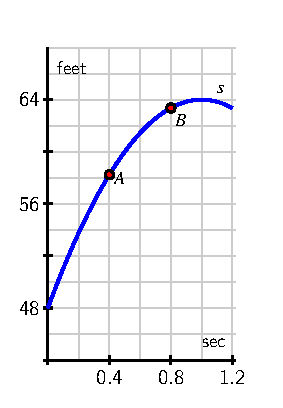
\includegraphics{figures/1_1_Act1.eps}
\caption{A partial plot of $s(t) = 64 - 16(t-1)^2$.} \label{F:1.1.Act1}
\end{center}
\end{figure}
\end{activity}
\begin{hint}[smallhint]
\begin{enumerate}
	\item On $[0.4,0.8]$, the average velocity is $AV_{[0.4,0.8]} = \frac{s(0.8)-s(0.4)}{0.8-0.4}$ ft/sec.
	\item Remember that the slope of a line can be found by taking ``rise over run.''  In this context, the slope is found by computing ``change in $s$ over change in $t$.''
	\item While the curve $s(t)$ is a parabola, how does it look up close on a very small interval? 
	\item ``Instantaneous'' velocity can be approximated by average velocity on a very small interval.
\end{enumerate}
\end{hint}
\begin{hint}[bighint]
\begin{enumerate}
	\item On $[0.4,0.8]$, the average velocity is $AV_{[0.4,0.8]} = \frac{s(0.8)-s(0.4)}{0.8-0.4}$ ft/sec.  Each of the other average velocities is computed similarly.
	\item Remember that the slope of a line can be found by taking ``rise over run.''  In this context, the slope is found by computing ``change in $s$ over change in $t$.''  Note that each average velocity $\frac{s(b)-s(a)}{b-a}$ can be viewed as the slope of a line between $(a,s(a))$ and $(b,s(b))$.
	\item While the curve $s(t)$ is a parabola, how does it look up close on a very small interval?  What type of familiar function seems to emerge?
	\item ``Instantaneous'' velocity can be approximated by average velocity on a very small interval.  Are the numbers you computed in (a) getting close to a particular value as we look at smaller and smaller intervals surrounding $t = 0.8$?
\end{enumerate}
\end{hint}
\begin{solution}
\begin{enumerate}
	\item On $[0.4,0.8]$, the average velocity is $AV_{[0.4,0.8]} = \frac{s(0.8)-s(0.4)}{0.8-0.4} = \frac{63.36-58.24}{0.4} = 12.8$ ft/sec.  On $[0.7,0.8]$, the average velocity is 8 ft/sec.  The other average velocities are, respectively (in the order of the intervals listed in the activity), 6.56, 6.416, 0, 4.8, 6.24, 6.384, all measured in feet per second.
	\item The slope of the line between $A(0.4, s(0.4))$ and $B(0.8, s(0.8))$ is $\frac{s(0.8)-s(0.4)}{0.8-0.4} = 12.8$.  This is precisely the average velocity of the ball between $t = 0.4$ and $t = 0.8$, and indeed each of the average velocities computed in (a) can be viewed as the slope of the line joining the points $(a,s(a))$ and $(b,s(b))$.
	\begin{center}
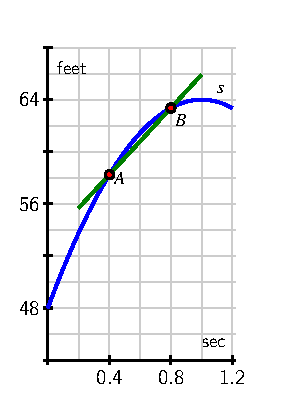
\includegraphics{figures/1_1_Act1Soln.eps}
\end{center}
	\item As we zoom in on the curve $s(t) = 64 - 16(t-1)^2$ at the point $(0.5, 60)$, the graph begins to look like a straight line.  Indeed, it appears to look like a straight line with slope about 6.4.
	\item Observe that the average velocity of the ball on the intervals $[0.799,0.8]$ and $[0.8,0.801]$ is 6.416 and 6.384 feet/sec respectively.  Hence it appears that the ball's velocity at the instant $t = 0.8$ should be about 6.4 feet per second.
\end{enumerate}
\end{solution}


\subsection*{Instantaneous Velocity}

Whether driving a car, riding a bike, or throwing a ball, we have an intuitive sense that any moving object has a velocity at any given moment -- a number that measures how fast the object is moving \emph{right now}.  For instance, a car's speedometer tells the driver what appears to be the car's velocity at any given instant.  In fact, the posted velocity on a speedometer is really an average velocity that is computed over a very small time interval (by computing how many revolutions the tires have undergone to compute distance traveled), since velocity fundamentally comes from considering a change in position divided by a change in time.  But if we let the time interval over which average velocity is computed become shorter and shorter, then we can progress from average velocity to \emph{instantaneous} velocity.  

Informally, we define the \emph{instantaneous velocity}\index{instantaneous velocity} of a moving object at time $t = a$ to be the value that the average velocity approaches as we take smaller and smaller intervals of time containing $t = a$ to compute the average velocity.  We will develop a more formal definition of this momentarily, one that will end up being the foundation of much of our work in first semester calculus.  For now, it is fine to think of instantaneous velocity this way:  take average velocities on smaller and smaller time intervals, and if those average velocities approach a single number, then that number will be the instantaneous velocity at that point.

\begin{activity}  \label{A:1.1.2}
Each of the following questions concern  $s(t) = 64 - 16(t-1)^2$, the position function from Preview Activity \ref{PA:1.1}.
\begin{enumerate}
	\item Compute the average velocity of the ball on the time interval $[1.5,2]$.  What is different between this value and the average velocity on the interval $[0,0.5]$?
	\item Use appropriate computing technology to estimate the instantaneous velocity of the ball at $t = 1.5$.  Likewise, estimate the instantaneous velocity of the ball at $t = 2$.  Which value is greater?
	\item How is the sign of the instantaneous velocity of the ball related to its behavior at a given point in time?  That is, what does positive instantaneous velocity tell you the ball is doing?  Negative instantaneous velocity?
	\item Without doing any computations, what do you expect to be the instantaneous velocity of the ball at $t = 1$?  Why?
\end{enumerate}
\end{activity}
\begin{hint}[smallhint]
\begin{enumerate}
	\item Remember to use the formula for average velocity from above:  $AV_{[a,b]} = \frac{s(b)-s(a)}{b-a}$.  Think carefully about whether certain quantities are positive or negative.
	\item To estimate the instantaneous velocity at $t = 1.5$, consider average velocities on the intervals $[1.499,1.5]$ and $[1.5,1.501]$.
	\item Think about whether the ball is rising or falling.
	\item What is the average velocity of the ball on small intervals that contain $t = 0$?
\end{enumerate}
\end{hint}
\begin{hint}[bighint]
\begin{enumerate}
	\item $AV_{[1.5,2]} = \frac{s(2)-s(1.5)}{2-1.5}$.  Your result should be negative since $s(2) < s(1.5)$.
	\item To estimate the instantaneous velocity at $t = 1.5$, consider average velocities on the intervals $[1.499,1.5]$ and $[1.5,1.501]$.
	\item You should find in (a) that the instantaneous velocity at $t = 1.5$ is negative, while earlier we found that the instantaneous velocity at $t = 0.5$ is positive.  How are these signs connected to whether the ball is rising or falling?
	\item Think about the line through the points $(0.999,s(0.999))$ and $(1,s(1))$ will look like given the ``special'' role of $(1,s(1))$ on the graph of $s(t)$.
\end{enumerate}
\end{hint}
\begin{solution}
\begin{enumerate}
	\item $AV_{[1.5,2]} = \frac{s(2)-s(1.5)}{2-1.5} = -24$ ft/sec.  We note that this average velocity is negative, and in fact is the opposite of the average velocity of 24 ft/sec on the interval $[0,0.5]$.
	\item Since $AV_{[1.499,1.5]} = -15.984$ and $AV_{[1.5, 1.501]} = -16.016$, it appears that the instantaneous velocity of the ball at $t = 1.5$ is approximately $-16$ ft/sec.  Similar computations show that at $t = 2$, it appears the instantaneous velocity is about $-32$ ft/sec.  Note that $-16>-32$, so the instantaneous velocity at $t = 1.5$ is greater because it is ``less negative.'' Asking which number is ``greater'' is different from asking which number is ``more negative.''
	\item When the ball is rising, its instantaneous velocity is positive, while when the ball is falling, its instantaneous velocity is negative.
	\item Note that $(1,s(1))$ is the vertex of the parabola given by $s(t)$.  At this point, the ball is neither rising nor falling.  On intervals of the form $[a,1]$, where $a < 1$, the average velocity of the ball is positive; on intervals of form $[1,b]$, where $b > 1$, the average velocity is positive.  Hence we expect the instantaneous velocity of the ball at the moment $t = 1$ to be zero.
\end{enumerate}
\end{solution}


At this point we have started to see a close connection between average velocity and instantaneous velocity, as well as how each is connected not only to the physical behavior of the moving object but also to the geometric behavior of the graph of the position function.  In order to make the link between average and instantaneous velocity more formal, we will introduce the notion of \emph{limit} in Section~\ref{S:1.2.Limits}.  As a preview of that concept, we look at a way to consider the limiting value of average velocity through the introduction of a parameter.  Note that if we desire to know the instantaneous velocity at $t = a$ of a moving object with position function $s$, we are interested in computing average velocities on the interval $[a,b]$ for smaller and smaller intervals.  One way to visualize this is to think of the value $b$ as being $b = a + h$, where $h$ is a small number that is allowed to vary.  Thus, we observe that the average velocity of the object on the interval $[a,a+h]$ is
$$AV_{[a,a+h]} = \frac{s(a+h)-s(a)}{h},$$
with the denominator being simply $h$ because $(a+h) - a = h$.  Initially, it is fine to think of $h$ being a small positive real number; but it is important to note that we allow $h$ to be a small negative number, too, as this enables us to investigate the average velocity of the moving object on intervals prior to $t = a$, as well as following $t = a$.  When $h < 0$, $AV_{[a,a+h]}$ measures the average velocity on the interval $[a+h,a]$.  

To attempt to find the instantaneous velocity at $t = a$, we investigate what happens as the value of $h$ approaches zero.  We consider this further in the following example.

\begin{example}
For a falling ball whose position function is given by $s(t) = 16 - 16t^2$ (where $s$ is measured in feet and $t$ in seconds), find an expression for the average velocity of the ball on a time interval of the form $[0.5, 0.5+h]$ where $-0.5 < h < 0.5$ and $h \ne 0$.  Use this expression to compute the average velocity on $[0.5,0.75]$ and $[0.4,0.5]$, as well as to make a conjecture about the instantaneous velocity at $t = 0.5$.
\end{example}
We make the assumptions that $-0.5 < h < 0.5$ and $h \ne 0$ because $h$ cannot be zero (otherwise there is no interval on which to compute average velocity) and because the function only makes sense on the time interval $0 \le t \le 1$, as this is the duration of time during which the ball is falling.  Observe that we want to compute and simplify $$AV_{[0.5, 0.5+h]} = \frac{s(0.5+h) - s(0.5)}{(0.5+h) - 0.5}.$$  The most unusual part of this computation is finding $s(0.5+h)$.  To do so, we follow the rule that defines the function $s$.  In particular, since $s(t) = 16-16t^2$, we see that \begin{eqnarray*}
  s(0.5+h) & = & 16 - 16(0.5 + h)^2 \\
  		& = & 16 - 16(0.25 + h + h^2) \\
		& = & 16 - 4 - 16h - 16h^2 \\
		& = & 12 - 16h - 16h^2.
\end{eqnarray*}
Now, returning to our computation of the average velocity, we find that 
\begin{eqnarray*}
 AV_{[0.5, 0.5+h]} & = & \frac{s(0.5+h) - s(0.5)}{(0.5+h) - 0.5} \\
 			& = & \frac{(12 - 16h - 16h^2) - (16 - 16(0.5)^2)}{0.5 + h - 0.5} \\
			& = & \frac{12 - 16h - 16h^2 - 12}{h} \\
			& = & \frac{-16h - 16h^2}{h}.
\end{eqnarray*}
At this point, we note two things:  first, the expression for average velocity clearly depends on $h$, which it must, since as $h$ changes the average velocity will change.  Further, we note that since $h$ can never equal zero, we may further simplify the most recent expression.  Removing the common factor of $h$ from the numerator and denominator, it follows that
$$ AV_{[0.5, 0.5+h]} = -16 - 16h.$$
Now, for any small positive or negative value of $h$, we can compute the average velocity.  For instance, to obtain the average velocity on $[0.5,0.75]$, we let $h = 0.25$, and the average velocity is $-16 - 16(0.25) = -20$ ft/sec.  To get the average velocity on $[0.4, 0.5]$, we let $h = -0.1$, which tells us the average velocity is $-16 - 16(-0.1) = -14.4$ ft/sec.  Moreover, we can even explore what happens to $AV_{[0.5, 0.5+h]}$ as $h$ gets closer and closer to zero.  As $h$ approaches zero, $-16h$ will also approach zero, and thus it appears that the instantaneous velocity of the ball at $t = 0.5$ should be $-16$ ft/sec.
\begin{center}\underline{}\end{center}


\begin{activity} \label{A:1.1.3}
For the function given by $s(t) = 64 - 16(t-1)^2$ from Preview Activity \ref{PA:1.1}, find the most simplified expression you can for the average velocity of the ball on the interval $[2, 2+h]$.  Use your result to compute the average velocity on $[1.5,2]$ and to estimate the instantaneous velocity at $t = 2$.  Finally, compare your earlier work in Activity~\ref{A:1.1.1}.
\end{activity} 
\begin{hint}[smallhint]
Note that $s(2+h) = 64 - 16(2+h-1)^2 = 64 - 16(1+h)^2 = 64 - (16 + 32h + 16h^2) = 48 - 32h - 16h^2$.
\end{hint}
\begin{hint}[bighint]
Note that $s(2+h) = 64 - 16(2+h-1)^2 = 64 - 16(1+h)^2 = 64 - (16 + 32h + 16h^2) = 48 - 32h - 16h^2$, and then recall that $AV_{[2, 2+h]} = \frac{s(2+h) - s(2)}{h}$.  Finally, you can use a negative value for $h$ to help you find the desired average velocity.
\end{hint}
\begin{solution}
Observe first that $s(2+h) = 64 - 16(2+h-1)^2 = 64 - 16(1+h)^2 = 64 - (16 + 32h + 16h^2) = 48 - 32h - 16h^2$.  Next, recall that $AV_{[2, 2+h]} = \frac{s(2+h) - s(2)}{h}$, so
$$AV_{[2, 2+h]} = \frac{s(2+h) - s(2)}{h} = \frac{(48 - 32h - 16h^2)-48}{h} = \frac{-32h - 16h^2}{h}.$$
Now, since we assume $h \ne 0$, we can simplify further to find that $AV_{[2, 2+h]} = -32 - 16h$.  Setting $h = -0.5$, it follows $AV_{[1.5,2]} = -32 + 16(0.5) = -24$ ft/sec, and letting $h$ approach zero, we see that $-32 - 16h$ will approach $-32$, so the instantaneous velocity at $t = 2$ appears to be $-32$ feet/sec.  Both results match our earlier work in Activity~\ref{A:1.1.1}.
\end{solution}


\begin{summary}
\item The average velocity on $[a,b]$ can be viewed geometrically as the slope of the line between the points $(a,s(a))$ and $(b,s(b))$ on the graph of $y = s(t)$, as shown in Figure~\ref{F:1.1.Summary}.
\begin{figure}[h]
\begin{center}
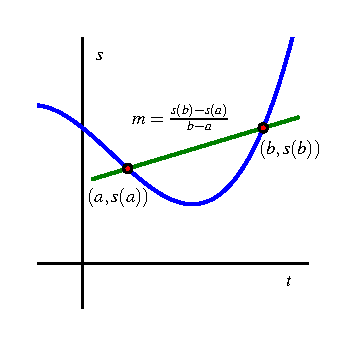
\includegraphics{figures/1_1_Summary.eps}
\caption{The graph of position function $s$ together with the line through $(a,s(a))$ and $(b,s(b))$ whose slope is $m = \frac{s(b)-s(a)}{b-a}$.  The line's slope is the average rate of change of $s$ on the interval $[a,b]$.} \label{F:1.1.Summary}
\end{center}
\end{figure}

\item Given a moving object whose position at time $t$ is given by a function $s$, the average velocity of the object on the time interval $[a,b]$ is given by $AV_{[a,b]} = \frac{s(b) - s(a)}{b-a}$.  Viewing the interval $[a,b]$ as having the form $[a,a+h]$, we equivalently compute average velocity by the formula $AV_{[a,a+h]} = \frac{s(a+h) - s(a)}{h}$.
\item The instantaneous velocity of a moving object at a fixed time is estimated by considering average velocities on shorter and shorter time intervals that contain the instant of interest.
\end{summary}



\begin{exercises}
\begin{enumerate}
\begin{enumerate} 

\item \label{Ez:1.1.1} A bungee jumper dives from a tower at time $t=0$.   Her height $h$ (measured in feet) at time $t$ (in seconds) is given by the graph in Figure~\ref{F:1.1.Ez1}.

\begin{figure}[h]
\begin{center}
 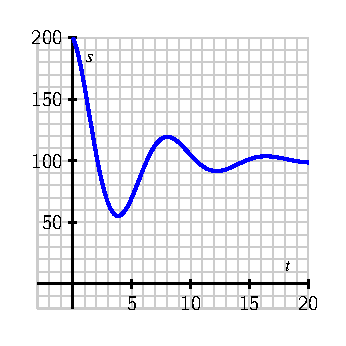
\includegraphics{figures/1_1_Ez1.eps}
 \caption{A bungee jumper's height function.} \label{F:1.1.Ez1}
\end{center}
\end{figure}

In this problem, you may base your answers on estimates from the graph or use the fact that the jumper's height function is given by $s(t) = 100\cos(0.75t) \cdot e^{-0.2t}+100$.
  \begin{enumerate}
	\item What is the change in vertical position of the bungee jumper between $t=0$ and $t=15$?
	\item Estimate the jumper's average velocity on each of the following time intervals:  $[0,15]$, $[0,2]$, $[1,6]$, and $[8,10]$.  Include units on your answers.
	\item On what time interval(s) do you think the bungee jumper achieves her greatest average velocity?  Why? 
	\item Estimate the jumper's instantaneous velocity at $t=5$.  Show your work and explain your reasoning, and include units on your answer.
	\item Among the average and instantaneous velocities you computed in earlier questions, which are positive and which are negative?  What does negative velocity indicate?
  \end{enumerate} 

\begin{solution}
\end{solution}
\item A diver leaps from a 3 meter springboard.  His feet leave the board at time $t=0$, he reaches his maximum height of 4.5 m at $t = 1.1$ seconds, and enters the water at $t = 2.45$.  Once in the water, the diver coasts to the bottom of the pool (depth 3.5 m), touches bottom at $t=7$, rests for one second, and then pushes off the bottom.  From there he coasts to the surface, and takes his first breath at $t=13$.

\begin{enumerate}
  \item Let $s(t)$ denote the function that gives the height of the diver's feet (in meters) above the water at time $t$.  (Note that the ``height'' of the bottom of the pool is $-3.5$ meters.)  Sketch a carefully labeled graph of $s(t)$ on the provided axes in Figure~\ref{F:1.1.Ez2}.  Include scale and units on the vertical axis.  Be as detailed as possible.

\begin{figure}[h]
  \begin{center}
 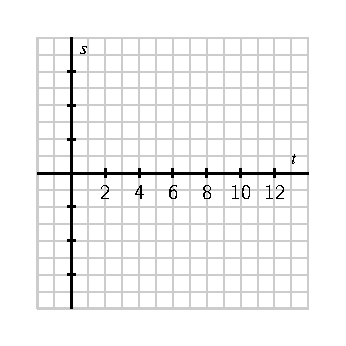
\includegraphics{figures/1_1_Ez2a.eps} \ \  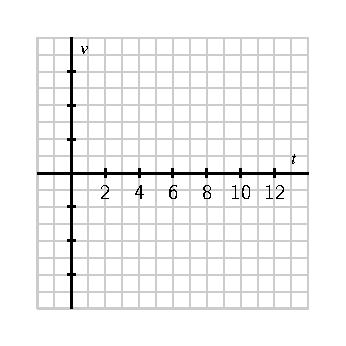
\includegraphics{figures/1_1_Ez2b.eps}
   \end{center}
   \caption{Axes for plotting $s(t)$ in part (a) and $v(t)$ in part (c) of the diver problem.} \label{F:1.1.Ez2}
\end{figure}

  \item Based on your graph in (a), what is the average velocity of the diver between $t = 2.45$ and $t=7$?  Is his average velocity the same on every time interval within $[2.45,7]$? 

  \item Let the function $v(t)$ represent the \emph{instantaneous vertical velocity} of the diver at time $t$ (i.e.~the speed at which the height function $s(t)$ is changing; note that velocity in the upward direction is positive, while the velocity of a falling object is negative).  Based on your understanding of the diver's behavior, as well as your graph of the position function, sketch a carefully labeled graph of $v(t)$ on the axes provided  in Figure~\ref{F:1.1.Ez2}.  Include scale and units on the vertical axis.  Write several sentences that explain how you constructed your graph, discussing when you expect $v(t)$ to be zero, positive, negative, relatively large, and relatively small.
  \item Is there a connection between the two graphs that you can describe?  What can you say about the velocity graph when the height function is increasing?  decreasing?  Make as many observations as you can.
\end{enumerate}
\begin{solution}
\end{solution}

\item According to the U.S. census, the population of the city of Grand Rapids, MI, was 181,843 in 1980; 189,126 in 1990; and 197,800 in 2000.

\begin{enumerate}
	\item Between 1980 and 2000, by how many people did the population of Grand Rapids grow?
	\item In an average year between 1980 and 2000, by how many people did the population of Grand Rapids grow?
	\item Just like we can find the average velocity of a moving body by computing change in position over change in time, we can compute the average rate of change of any function $f$.  In particular, the \emph{average rate of change} of a function $f$ over an interval $[a,b]$ is the quotient
$$\frac{f(b)-f(a)}{b-a}.$$  
What does the quantity $\frac{f(b)-f(a)}{b-a}$ measure on the graph of $y = f(x)$ over the interval $[a,b]$?
	\item Let $P(t)$ represent the population of Grand Rapids at time $t$, where $t$ is measured in years from January 1, 1980.  What is the average rate of change of $P$ on the interval $t = 0$ to $t = 20$?  What are the units on this quantity?
	\item If we assume the population of Grand Rapids is growing at a rate of approximately 4\% per decade,  we can model the population function with the formula $$P(t) = 181843 (1.04)^{t/10}.$$  Use this formula to compute the average rate of change of the population on the intervals $[5,10]$, $[5,9]$, $[5,8]$, $[5,7]$, and $[5,6]$.
	\item How fast do you think the population of Grand Rapids was changing on January 1, 1985?  Said differently, at what rate do you think people were being added to the population of Grand Rapids as of January 1, 1985?  How many additional people should the city have expected in the following year?  Why?
\end{enumerate}

\end{enumerate}
\end{enumerate}
\end{exercises}
 

\clearpage
\section{The notion of limit} \label{S:1.2.Limits}

\vspace{-14 pt}

In this section, we strive to understand the ideas generated by the following important questions:
\begin{objectives}
\begin{itemize}
\item What is the mathematical notion of \emph{limit} and what role do limits play in the study of functions?
\item What is the meaning of the notation $\ds \lim_{x \to a} f(x) = L$?
\item How do we go about determining the value of the limit of a function at a point?
\item How does the notion of limit allow us to move from average velocity to instantaneous velocity?
\end{itemize}\end{objectives} 

\subsection*{Introduction}

Functions are at the heart of mathematics: a function is a process or rule that associates each individual input to exactly one corresponding output.  Students learn in courses prior to calculus that there are many different ways to represent functions, including through formulas, graphs, tables, and even words.  For example, the squaring function can be thought of in any of these ways.  In words, the squaring function takes any real number $x$ and computes its square.  The formulaic and graphical representations go hand in hand, as $y = f(x) = x^2$ is one of the simplest curves to graph.  Finally, we can also partially represent this function through a table of values, essentially by listing some of the ordered pairs that lie on the curve, such as  $(-2,4)$, $(-1,1)$, $(0,0)$, $(1,1)$, and $(2,4)$.

Functions are especially important in calculus because they often model important phenomena -- the location of a moving object at a given time, the rate at which an automobile is consuming gasoline at a certain velocity, the reaction of a patient to the size of a dose of a drug -- and calculus can be used to study how these output quantities change in response to changes in the input variable.  Moreover, thinking about concepts like average and instantaneous velocity leads us naturally from an initial function to a related, sometimes more complicated function.  As one example of this, think about the falling ball whose position function is given by $s(t) = 64 - 16t^2$ and the average velocity of the ball on the interval $[1,x]$.  Observe that
$$AV_{[1,x]} = \frac{s(x) - s(1)}{x-1} = \frac{(64-16x^2) - (64-16)}{x-1} = \frac{16 - 16x^2}{x-1}.$$
Now, two things are essential to note:  this average velocity depends on $x$ (indeed, $AV_{[1,x]}$ is a function of $x$), and our most focused interest in this function occurs near $x = 1$, which is where the function is not defined.  Said differently, the function $g(x) = \frac{16 - 16x^2}{x-1}$ tells us the average velocity of the ball on the interval from $t = 1$ to $t = x$, and if we are interested in the instantaneous velocity of the ball when $t = 1$, we'd like to know what happens to $g(x)$ as $x$ gets closer and closer to $1$.  At the same time, $g(1)$ is not defined, because it leads to the quotient $0/0$.

This is where the idea of \emph{limits} comes in.  By using a limit, we'll be able to allow $x$ to get arbitrarily close, but not equal, to $1$ and fully understand the behavior of $g(x)$ near this value.  We'll develop key language, notation, and conceptual understanding in what follows, but for now we consider a preliminary activity that uses the graphical interpretation of a function to explore points on a graph where interesting behavior occurs.

\begin{previewactivity} \label{PA:1.2}
Suppose that $g$ is the function given by the graph below.  Use the graph to answer each of the following questions. 
\begin{enumerate}
	\item Determine the values $g(-2)$, $g(-1)$, $g(0)$, $g(1)$, and $g(2)$, if defined.  If the function value is not defined, explain what feature of the graph tells you this.
	\item For each of the values $a = -1$, $a = 0$, and $a = 2$, complete the following sentence: ``As $x$ gets closer and closer (but not equal) to $a$, $g(x)$ gets as close as we want to \underline{}.''
	\item What happens as $x$ gets closer and closer (but not equal) to $a = 1$?  Does the function $g(x)$ get as close as we would like to a single value?
\end{enumerate}

\begin{figure}[h]
\begin{center}
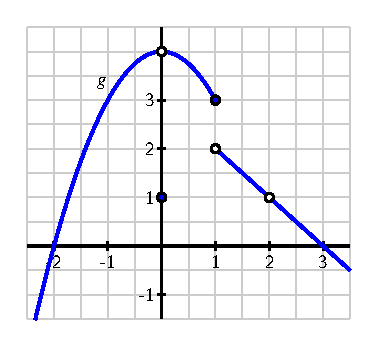
\includegraphics{figures/1_2_PA1.eps} 
\caption{Graph of $y = g(x)$ for Preview Activity~\ref{PA:1.2}.} \label{F:1.2.PA1}
\end{center}
\end{figure}

\end{previewactivity}

\subsection*{The Notion of Limit}

Limits can be thought of as a way to study the tendency or trend of a function as the input variable approaches a fixed value, or even as the input variable increases or decreases without bound.  We put off the study of the latter idea until further along in the course when we will have some helpful calculus tools for understanding the end behavior of functions.  Here, we focus on what it means to say that ``a function $f$ has limit $L$ as $x$ approaches $a$.''  To begin, we think about a recent example.

In Preview Activity \ref{PA:1.2}, you saw that for the given function $g$, as $x$ gets closer and closer (but not equal) to 0, $g(x)$ gets as close as we want to the value 4.  At first, this may feel counterintuitive, because the value of $g(0)$ is $1$, not $4$.  By their very definition, limits regard the behavior of a function \emph{arbitrarily close to} a fixed input, but the value of the function \emph{at} the fixed input does not matter.  More formally\footnote{What follows here is not what mathematicians consider the formal definition of a limit.  To be completely precise, it is necessary to quantify both what it means to say ``as close to $L$ as we like'' and ``sufficiently close to $a$.''  That can be accomplished through what is traditionally called the epsilon-delta definition of limits.  The definition presented here is sufficient for the purposes of this text.}, we say the following.

\begin{definition}
Given a function $f$, a fixed input $x = a$, and a real number $L$, we say that \emph{$f$ has limit\index{limit!definition} $L$ as $x$ approaches $a$}, and write
$$\lim_{x \to a} f(x) = L$$
provided that we can make $f(x)$ as close to $L$ as we like by taking $x$ sufficiently close (but not equal) to $a$.  If we cannot make $f(x)$ as close to a single value as we would like as $x$ approaches $a$, then we say that \emph{$f$ does not have a limit as $x$ approaches $a$.}
\end{definition}
For the function $g$ pictured in Figure \ref{F:1.2.PA1}, we can make the following observations:  
$$\ds \lim_{x \to -1} g(x) = 3, \ \ds \lim_{x \to 0} g(x) = 4, \ \mbox{and} \ \ds \lim_{x \to 2} g(x) = 1,$$ but $g$ does not have a limit as $x \to 1$.  When working graphically, it suffices to ask if the function approaches a single value from each side of the fixed input, while understanding that the function value right at the fixed input is irrelevant.  This reasoning explains the values of the first three stated limits.  In a situation such as the jump in the graph of $g$ at $x = 1$, the issue is that if we approach $x = 1$ from the left, the function values tend to get as close to 3 as we'd like, but if we approach $x = 1$ from the right, the function values get as close to 2 as we'd like, and there is no single number that all of these function values approach.  This is why the limit of $g$ does not exist at $x = 1$.

For any function $f$, there are typically three ways to answer the question ``does $f$ have a limit at $x = a$, and if so, what is the limit?''  The first is to reason graphically as we have just done with the example from Preview Activity \ref{PA:1.2}.  If we have a formula for $f(x)$, there are two additional possibilities:  (1) evaluate the function at a sequence of inputs that approach $a$ on either side, typically using some sort of computing technology, and ask if the sequence of outputs seems to approach a single value; (2) use the algebraic form of the function to understand the trend in its output as the input values approach $a$.  The first approach only produces an approximation of the value of the limit, while the latter can often be used to determine the limit exactly.  The following example demonstrates both of these approaches, while also using the graphs of the respective functions to help confirm our conclusions.

\begin{example} \label{Ex:1.2.Limits}
For each of the following functions, we'd like to know whether or not the function has a limit at the stated $a$-values.  Use both numerical and algebraic approaches to investigate and, if possible, estimate or determine the value of the limit.  Compare the results with a careful graph of the function on an interval containing the points of interest.
\begin{enumerate}
	\item $\ds f(x) = \frac{4-x^2}{x+2}$; $a = -1$, $a = -2$
	\item $\ds g(x) = \sin\left(\frac{\pi}{x}\right)$; $a = 3$, $a = 0$
\end{enumerate}
\end{example}
We first construct a graph of $f$ along with tables of values near $a = -1$ and $a = -2$.  

\begin{figure}[h]

\begin{tabular}{ccc}
	\raisebox{.5in}{\begin{tabular}[b]{r|l} $x$ & $f(x)$ \\ \hline -0.9 & 2.9 \\ -0.99 & 2.99 \\ -0.999 & 2.999 \\ -0.9999 & 2.9999 \\ -1.1 & 3.1 \\ -1.01 & 3.01 \\ -1.001 & 3.001 \\ -1.0001 & 3.0001  \end{tabular} } &	
	\raisebox{.5in}{\begin{tabular}[b]{r|l} $x$ & $f(x)$ \\ \hline -1.9 & 3.9 \\ -1.99 & 3.99 \\ -1.999 & 3.999 \\ -1.9999 & 3.9999 \\ -2.1 & 4.1 \\ -2.01 & 4.01 \\ -2.001 & 4.001 \\ -2.0001 & 4.0001  \end{tabular} } &
	 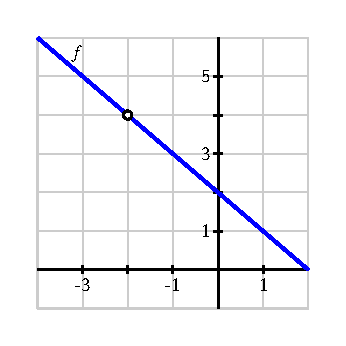
\includegraphics{figures/1_2_Ex1f.eps} 
\end{tabular}
\caption{Tables and graph for $\ds f(x) = \frac{4-x^2}{x+2}$. } \label{F:1.2.Ex1f}
\end{figure}

From the left table, it appears that we can make $f$ as close as we want to 3 by taking $x$ sufficiently close to $-1$, which suggests that $\ds \lim_{x \to -1} f(x) = 3$.	This is also consistent with the graph of $f$.  To see this a bit more rigorously and from an algebraic point of view, consider the formula for $f$:  $f(x) = \frac{4-x^2}{x+2}$.  The numerator and denominator are each polynomial functions, which are among the most well-behaved functions that exist.  Formally, such functions are \emph{continuous}\footnote{See Section~\ref{S:1.7.LimContDiff} for more on the notion of continuity.}, which means that the limit of the function at any point is equal to its function value.  Here, it follows that as $x \to -1$,  $(4-x^2) \to (4 - (-1)^2) = 3$, and $(x+2) \to (-1 + 2) = 1$, so as $x \to -1$, the numerator of $f$ tends to 3 and the denominator tends to 1, hence $\ds \lim_{x \to -1} f(x) = \frac{3}{1} = 3$.

The situation is more complicated when $x \to -2$, due in part to the fact that $f(-2)$ is not defined.  If we attempt to use a similar algebraic argument regarding the numerator and denominator, we observe that as $x \to -2$, $(4-x^2) \to (4 - (-2)^2) = 0$, and $(x+2) \to (-2 + 2) = 0$, so as $x \to -2$, the numerator of $f$ tends to 0 and the denominator tends to 0.  We call $0/0$ an \emph{indeterminate form}\index{indeterminate} and will revisit several important issues surrounding such quantities later in the course.  For now, we simply observe that this tells us there is somehow more work to do.  From the table and the graph, it appears that $f$ should have a limit of $4$ at $x = -2$.  To see algebraically why this is the case, let's work directly with the form of $f(x)$.  Observe that
\begin{eqnarray*}
	\lim_{x \to -2} f(x) & = & \lim_{x \to -2} \frac{4-x^2}{x+2} \\
				& = & \lim_{x \to -2} \frac{(2-x)(2+x)}{x+2}. 
\end{eqnarray*}
At this point, it is important to observe that since we are taking the limit as $x \to -2$, we are considering $x$ values that are close, but not equal, to $-2$.  Since we never actually allow $x$ to equal $-2$, the quotient $\frac{2+x}{x+2}$ has value 1 for every possible value of $x$.  Thus, we can simplify the most recent expression above, and now find that
$$\lim_{x \to -2} f(x) = \lim_{x \to -2} 2-x.$$
Because $2-x$ is simply a linear function, this limit is now easy to determine, and its value clearly is $4$.  Thus, from several points of view we've seen that $\ds\lim_{x \to -2} f(x) = 4.$

Next we turn to the function $g$, and construct two tables and a graph.
\begin{figure}[h]

\begin{tabular}{ccc}
	\raisebox{-.05in}{\begin{tabular}[b]{r|l} $x$ & $g(x)$ \\ \hline 2.9 & 0.84864 \\ 2.99 & 0.86428 \\ 2.999 & 0.86585 \\ 2.9999 & 0.86601 \\ 3.1 & 0.88351 \\ 3.01 &  0.86777 \\ 3.001 & 0.86620 \\ 3.0001 &  0.86604  \end{tabular} } &	
	\raisebox{-.05in}{\begin{tabular}[b]{r|l} $x$ & $g(x)$ \\ \hline -0.1 & 0 \\ -0.01 & 0 \\ -0.001 & 0 \\ -0.0001 & 0 \\ 0.1 & 0 \\ 0.01 & 0 \\ 0.001 & 0 \\ 0.0001 & 0  \end{tabular} } &
	 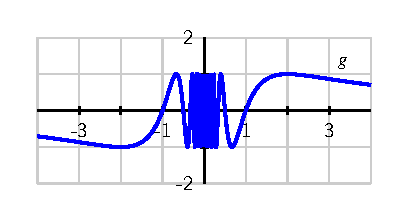
\includegraphics{figures/1_2_Ex1g.eps} 
\end{tabular}
\caption{Tables and graph for $\ds g(x) = \sin\left(\frac{\pi}{x}\right)$.} \label{F:1.2.Ex1g}
\end{figure}

First, as $x \to 3$, it appears from the data (and the graph) that the function is approaching approximately $0.866025$.  To be precise, we have to use the fact that $\frac{\pi}{x} \to \frac{\pi}{3}$, and thus we find that $g(x) = \sin(\frac{\pi}{x}) \to \sin(\frac{\pi}{3})$ as $x \to 3$.  The exact value of $\sin(\frac{\pi}{3})$ is $\frac{\sqrt{3}}{2}$, which is approximately 0.8660254038.  Thus, we see that
$$\lim_{x \to 3} g(x) = \frac{\sqrt{3}}{2}.$$

As $x \to 0$, we observe that $\frac{\pi}{x}$ does not behave in an elementary way.  When $x$ is positive and approaching zero, we are dividing by smaller and smaller positive values, and $\frac{\pi}{x}$ increases without bound.  When $x$ is negative and approaching zero, $\frac{\pi}{x}$ decreases without bound.  In this sense, as we get close to $x = 0$, the inputs to the sine function are growing rapidly, and this leads to wild oscillations in the graph of $g$.  It is an instructive exercise to plot the function $g(x) = \sin\left(\frac{\pi}{x}\right)$ with a graphing utility and then zoom in on $x = 0$.  Doing so shows that the function never settles down to a single value near the origin and suggests that $g$ does not have a limit at $x = 0$.

How do we reconcile this with the righthand table above, which seems to suggest that the limit of $g$ as $x$ approaches $0$ may in fact be $0$?  Here we need to recognize that the data misleads us because of the special nature of the sequence $\{0.1, 0.01, 0.001, \ldots\}$: when we evaluate $g(10^{-k})$, we get $g(10^{-k}) = \sin\left(\frac{\pi}{10^{-k}}\right) = \sin(10^k \pi) = 0$ for each positive integer value of $k$.  But if we take a different sequence of values approaching zero, say $\{0.3, 0.03, 0.003, \ldots\}$, then we find that 
$$g(3 \cdot 10^{-k}) = \sin\left(\frac{\pi}{3 \cdot 10^{-k}}\right) = \sin\left(\frac{10^k \pi}{3}\right) = \frac{\sqrt{3}}{2} \approx 0.866025.$$
That sequence of data would suggest that the value of the limit is $\frac{\sqrt{3}}{2}$.  Clearly the function cannot have two different values for the limit, and this shows that $g$ has no limit as $x \to 0$.
\begin{center}\underline{}\end{center}

An important lesson to take from Example~\ref{Ex:1.2.Limits} is that tables can be misleading when determining the value of a limit.  While a table of values is useful for investigating the possible value of a limit, we should also use other tools to confirm the value, if we think the table suggests the limit exists.

\begin{activity} \label{A:1.2.1}  Estimate the value of each of the following limits by constructing appropriate tables of values.  Then determine the exact value of the limit by using algebra to simplify the function. Finally, plot each function on an appropriate interval to check your result visually.
\begin{enumerate}
		\item $\ds \lim_{x \to 1} \frac{x^2 - 1}{x-1}$
		\item $\ds \lim_{x \to 0} \frac{(2+x)^3 - 8}{x}$
		\item $\ds \lim_{x \to 0} \frac{\sqrt{x+1} - 1}{x}$
\end{enumerate}
\end{activity}
\begin{hint}[smallhint]
\begin{enumerate}
	\item $(x^2 - 1)$ can be factored.
	\item Expand the expression $(2+x)^3$, and then combine like terms in the numerator.
	\item Try multiplying the given function by this fancy form of 1: $\frac{\sqrt{x+1} + 1}{\sqrt{x+1} + 1}$.
\end{enumerate}
\end{hint}
\begin{hint}[bighint]
\begin{enumerate}
	\item $(x^2 - 1) = (x+1)(x-1)$.
	\item Expand the expression $(2+x)^3$ using the rule $(a+b)^3 = a^3 + 3a^2b + 3ab^2 + b^3$, and then combine like terms in the numerator.
	\item Try multiplying the given function by this fancy form of 1: $\frac{\sqrt{x+1} + 1}{\sqrt{x+1} + 1}$.  Expand and simplify the numerator, and then see what happens as $x \to 0$.
\end{enumerate}
\end{hint}
\begin{solution}
Estimating the values of the limits with tables is straightforward and should suggest the exact values stated below.
\begin{enumerate}
	\item $\ds \lim_{x \to 1} \frac{x^2 - 1}{x-1} = \lim_{x \to 1} \frac{(x+1)(x-1)}{x-1} = \lim_{x \to 1} (x+1) = 2$. 
	\item $\ds \lim_{x \to 0} \frac{(2+x)^3 - 8}{x} = \lim_{x \to 0} \frac{8 + 12x + 6x^2 + x^3 - 8}{x} = \lim_{x \to 0} \frac{12x + 6x^2 + x^3}{x} =  \lim_{x \to 0} (12 + 6x + x^2) = 12$.
	\item $\ds \lim_{x \to 0} \frac{\sqrt{x+1} - 1}{x} = \lim_{x \to 0} \frac{\sqrt{x+1} - 1}{x} \cdot \frac{\sqrt{x+1} + 1}{\sqrt{x+1} + 1} = \lim_{x \to 0} \frac{x+1-1}{x(\sqrt{x+1}+1)} = \lim_{x \to 0} \frac{1}{\sqrt{x+1}+1} = \frac{1}{2}.$
\end{enumerate}
\end{solution}



This concludes a rather lengthy introduction to the notion of limits.  It is important to remember that our primary motivation for considering limits of functions comes from our interest in studying the rate of change of a function.  To that end, we close this section by revisiting our previous work with average and instantaneous velocity and highlighting the role that limits play. 

\subsection*{Instantaneous Velocity}

Suppose that we have a moving object whose position at time $t$ is given by a function $s$.  We know that the average velocity of the object on the time interval $[a,b]$ is $AV_{[a,b]} = \frac{s(b)-s(a)}{b-a}.$  We define the \emph{instantaneous velocity} \index{instantaneous velocity} at $a$ to be the limit of average velocity as $b$ approaches $a$.  Note particularly that as $b \to a$, the length of the time interval gets shorter and shorter (while always including $a$).  In Section~\ref{S:1.3.DerivativePt}, we will introduce a helpful shorthand notation to represent the instantaneous rate of change.  For now, we will write $IV_{t=a}$ for the instantaneous velocity at $t = a$, and thus
$$IV_{t=a} = \lim_{b \to a} AV_{[a,b]} = \lim_{b \to a} \frac{s(b)-s(a)}{b-a}.$$
Equivalently, if we think of the changing value $b$ as being of the form $b = a + h$, where $h$ is some small number, then we may instead write
$$IV_{t=a} = \lim_{h \to 0} AV_{[a,a+h]} = \lim_{h \to 0} \frac{s(a+h)-s(a)}{h}.$$
Again, the most important idea here is that to compute instantaneous velocity\index{instantaneous velocity}, we take a limit of average velocities as the time interval shrinks.  Two different activities offer the opportunity to investigate these ideas and the role of limits further. \\

\begin{activity}  \label{A:1.2.2}
Consider a moving object whose position function is given by $s(t) = t^2$, where $s$ is measured in meters and $t$ is measured in minutes.  
\begin{enumerate}
	\item Determine the most simplified expression for the average velocity of the object on the interval $[3, 3+h]$, where $h > 0$.
	\item Determine the average velocity of the object on the interval $[3,3.2]$.  Include units on your answer.
	\item Determine the instantaneous velocity of the object when $t = 3$.  Include units on your answer.
\end{enumerate}
\end{activity}
\begin{hint}[smallhint]
\begin{enumerate}
	\item $s(3+h) = (3+h)^2$.
	\item Recall that $AV_{[a,b]} = \frac{s(b)-s(a)}{b-a}$.
	\item Consider $\lim_{h \to 0} \frac{s(3+h)-s(3)}{h}$ and use your work in (a).
\end{enumerate}
\end{hint}
\begin{hint}[bighint]
\begin{enumerate}
	\item $s(3+h) = (3+h)^2 = 9 + 6h + h^2$; show that $s(3+h) - s(3) = 6h + h^2$.
	\item Compute $AV_{[3,3.2]} = \frac{s(3.2)-s(3)}{3.2-3}$.
	\item Consider $\lim_{h \to 0} \frac{s(3+h)-s(3)}{h} = \lim_{h \to 0} \frac{6h + h^2}{h}$.
\end{enumerate}
\end{hint}
\begin{solution}
\begin{enumerate}
	\item Observe that $AV_{[3, 3+h]} =  \frac{s(3+h)-s(3)}{h} = \frac{(3+h)^2 - 3^2}{h} = \frac{9 + 6h + h^2 - 9}{h} = \frac{6h + h^2}{h} = \frac{h(6 + h)}{h} = 6 + h.$
	\item Using the expression just found in (a) with $h = 0.2$, $AV_{[3,3.2]} = 6 + 0.2 = 6.2$ meters/min.
	\item Taking the limit of average velocity and using our work from (a), we find that
	$$IV_{t = 3} = \lim_{h \to 0} AV_{[3, 3+h]} = \lim_{h \to 0} 6+h = 6,$$
	so the instantaneous velocity of the object when $t = 3$ is 6 meters per minute.
\end{enumerate}
\end{solution}


 The closing activity of this section asks you to make some connections among average velocity, instantaneous velocity, and slopes of certain lines.

\begin{activity} \label{A:1.2.3}
For the moving object whose position $s$ at time $t$ is given by the graph below, answer each of the following questions.  Assume that $s$ is measured in feet and $t$ is measured in seconds.
\begin{figure}[h]
\begin{center}
 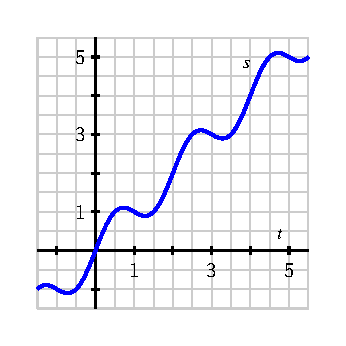
\includegraphics{figures/1_2_Act3.eps} \caption{Plot of the position function $y = s(t)$ in Activity~\ref{A:1.2.3}.}
\end{center}
\end{figure}
\begin{enumerate}
	\item Use the graph to estimate the average velocity of the object on each of the following intervals: $[0.5,1]$, $[1.5,2.5]$, $[0,5]$.  Draw each line whose slope represents the average velocity you seek.
	\item How could you use average velocities or slopes of lines to estimate the instantaneous velocity of the object at a fixed time?
	\item Use the graph to estimate the instantaneous velocity of the object when $t = 2$.  Should this instantaneous velocity at $t = 2$ be greater or less than the average velocity on $[1.5,2.5]$ that you computed in (a)?  Why?
\end{enumerate}
\end{activity} 
\begin{hint}[smallhint]
\begin{enumerate}
	\item Remember that average velocity on an interval computes the quotient of ``change in $s$ over change in $t$.''  This is the slope of the line between the corresponding two points on the graph of $s$.
	\item Think about shorter and shorter time intervals and drawing the lines whose slopes represent average velocity.
	\item Think about zooming in on the graph at $t = 2$ and drawing a line that, up close, looks just like the curve $s(t)$.  What is the approximate slope of that line?
\end{enumerate}
\end{hint}
\begin{hint}[bighint]
\begin{enumerate}
	\item Remember that average velocity on an interval computes the quotient of ``change in $s$ over change in $t$.''  This is the slope of the line between the corresponding two points on the graph of $s$.  For example, the average velocity on $[0.5,1]$ is $\frac{1-1}{1-0.5} = 0$.
	\item Think about shorter and shorter time intervals and drawing the lines whose slopes represent average velocity.  If those lines' slopes are approaching a single number, that number represents the instantaneous velocity.
	\item Think about zooming in on the graph at $t = 2$ and drawing a line that, up close, looks just like the curve $s(t)$.  What is the approximate slope of that line?  By drawing this line that looks like $s(t)$ near the point $(2,s(2))$ and comparing the line through the points $(1.5,s(1.5))$ and $(2.5, s(2.5))$, you should be able to compare the lines and see which has greater slope.
\end{enumerate}
\end{hint}
\begin{solution}
\begin{enumerate}
	\item The average velocity on $[0.5,1]$ is the slope of the line joining the points $(0.5,s(0.5))$ and $(1,s(1))$, which is $AV_{[0.5,1]} = \frac{1-1}{1-0.5} = 0$.  On $[1.5,2.5]$, we similarly find $AV_{[1.5,2.5]} = \frac{3-1}{2.5-1.5} = 2$, and on $[0,5]$, we have $AV_{[0,5]} = \frac{5-0}{5-0} = 1$.
	\item  Take shorter and shorter time intervals and draw the lines whose slopes represent average velocity.  If those lines' slopes are approaching a single number, that number represents the instantaneous velocity.  For example, to estimate the instantaneous velocity at $t = 2$, we might consider average velocities on $[2,3]$, $[2,2.5]$, and $[2,2.25]$.
	\item  If we draw the line through $(2,2)$ and $(2.1,s(2.1))$, it looks like the line's slope is approximately 2.5: if we go over one grid-width, we appear to go up about 2.5.  The slope of this line is clearly greater than the slope of the line through $(1.5, s(1.5))$ and $(2.5, s(2.5))$, which is 2. Hence the instantaneous velocity at $t = 2$ is greater than the average velocity on $[1.5,2.5]$.
\end{enumerate}
\end{solution}


\begin{authornote}
This is an author note.
\end{authornote}


\begin{summary}
\item Limits enable us to examine trends in function behavior near a specific point.  In particular, taking a limit at a given point asks if the function values nearby tend to approach a particular fixed value.
\item When we write $\ds \lim_{x \to a} f(x) = L$, we read this as saying ``the limit of $f$ as $x$ approaches $a$ is $L$,'' and this means that we can make the value of $f(x)$ as close to $L$ as we want by taking $x$ sufficiently close (but not equal) to $a$.
\item If we desire to know $\ds \lim_{x \to a} f(x)$ for a given value of $a$ and a known function $f$, we can estimate this value from the graph of $f$ or by generating a table of function values that result from a sequence of $x$-values that are closer and closer to $a$.  If we want the exact value of the limit, we need to work with the function algebraically and see if we can use familiar properties of known, basic functions to understand how different parts of the formula for $f$ change as $x \to a$. 
\item The instantaneous velocity of a moving object at a fixed time is found by taking the limit of average velocities of the object over shorter and shorter time intervals that all contain the time of interest.
\end{summary}



\begin{exercises}
\begin{enumerate}
\begin{enumerate} 
\item Consider the function whose formula is $\ds f(x) = \frac{16-x^4}{x^2-4}$.
  \begin{enumerate}
  	\item What is the domain of $f$?
	\item Use a sequence of values of $x$ near $a = 2$ to estimate the value of $\ds \lim_{x \to 2} f(x),$
	if you think the limit exists.  If you think the limit doesn't exist, explain why.
	\item Use algebra to simplify the expression $\frac{16-x^4}{x^2-4}$ and hence work to evaluate $\lim_{x \to 2} f(x)$ exactly, if it exists, or to explain how your work shows the limit fails to exist.  Discuss how your findings compare to your results in (b).
	\item True or false: $f(2) = -8$.  Why?
	\item True or false: $\frac{16-x^4}{x^2-4} = -4-x^2.$  Why?  How is this equality connected to your work above with the function $f$?
	\item Based on all of your work above, construct an accurate, labeled graph of $y = f(x)$ on the interval $[1,3]$, and write a sentence that explains what you now know about $\ds \lim_{x \to 2} \frac{16-x^4}{x^2-4}$.
  \end{enumerate}
 
\begin{solution}
\end{solution}
\item  Let $\ds g(x) = -\frac{|x+3|}{x+3}$.
  \begin{enumerate}
  	\item What is the domain of $g$?
	\item Use a sequence of values near $a = -3$ to estimate the value of
	$\lim_{x \to -3} g(x),$
	if you think the limit exists.  If you think the limit doesn't exist, explain why. 
	\item Use algebra to simplify the expression $\frac{|x+3|}{x+3}$ and hence work to evaluate $\lim_{x \to -3} g(x)$ exactly, if it exists, or to explain how your work shows the limit fails to exist.  Discuss how your findings compare to your results in (b).  (\textbf{Hint}: $|a| = a$ whenever $a \ge 0$, but $|a| = -a$ whenever $a < 0$.)
	\item True or false: $g(-3) = -1$.  Why?
	\item True or false: $-\frac{|x+3|}{x+3} = -1.$  Why?  How is this equality connected to your work above with the function $g$?
	\item Based on all of your work above, construct an accurate, labeled graph of $y = g(x)$ on the interval $[-4,-2]$, and write a sentence that explains what you now know about $\ds \lim_{x \to -3} g(x)$.
  \end{enumerate}


\item For each of the following prompts, sketch a graph on the provided axes of a function that has the stated properties.
\begin{figure}[h]
  \begin{center}
 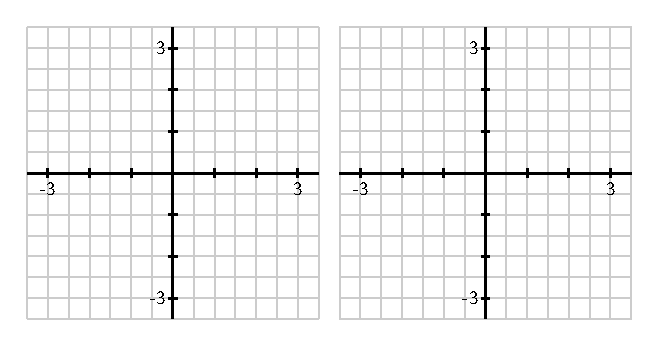
\includegraphics{figures/1_2_Ez3.eps} 
   \end{center}
   \caption{Axes for plotting $y = f(x)$ in (a) and $y = g(x)$ in (b).} \label{F:1.2.Ez3}
\end{figure}
  \begin{enumerate}
  	\item $y = f(x)$ such that 
	\begin{itemize}
		\item $f(-2) = 2$ and $\ds \lim_{x \to -2} f(x) = 1$
		\item $f(-1) = 3$ and $\ds \lim_{x \to -1} f(x) = 3$
		\item $f(1)$ is not defined and $\ds \lim_{x \to 1} f(x) = 0$
		\item $f(2) = 1$ and $\ds \lim_{x \to 2} f(x)$ does not exist.
	\end{itemize}
	\item $y = g(x)$ such that
	\begin{itemize}
		\item $g(-2) = 3$, $g(-1) = -1$, $g(1) = -2$, and $g(2) = 3$
		\item At $x = -2, -1, 1$ and $2$, $g$ has a limit, and its limit equals the value of the function at that point.
		\item $g(0)$ is not defined and $\ds \lim_{x \to 0} g(x)$ does not exist.
	\end{itemize}

  \end{enumerate}

\item A bungee jumper dives from a tower at time $t=0$. Her height  $s$ in feet at time $t$ in seconds is given by $s(t) = 100\cos(0.75t) \cdot e^{-0.2t}+100$.
	\begin{enumerate}
		\item Write an expression for the average velocity of the bungee jumper on the interval \\ $[1,1+h]$.
		\item Use computing technology to estimate the value of the limit as $h \to 0$ of the quantity you found in (a).
		\item What is the meaning of the value of the limit in (b)?  What are its units?
	\end{enumerate}

\end{enumerate}
\end{enumerate}
\end{exercises} 

\clearpage
\section{The derivative of a function at a point} \label{S:1.3.DerivativePt}

\vspace{-14 pt}

In this section, we strive to understand the ideas generated by the following important questions:
\begin{objectives}
\begin{itemize}
\item How is the average rate of change of a function on a given interval defined, and what does this quantity measure?
\item How is the instantaneous rate of change of a function at a particular point defined?  How is the instantaneous rate of change linked to average rate of change?
\item What is the derivative of a function at a given point?  What does this derivative value measure? How do we interpret the derivative value graphically?
\item How are limits used formally in the computation of derivatives?
\end{itemize}\end{objectives} 

\subsection*{Introduction}

An idea that sits at the foundations of calculus is the \emph{instantaneous rate of change} of a function.  This rate of change is always considered with respect to change in the input variable, often at a particular fixed input value.  This is a generalization of the notion of instantaneous velocity and essentially allows us to consider the question ``how do we measure how fast a particular function is changing at a given point?''  When the original function represents the position of a moving object, this instantaneous rate of change is precisely velocity, and might be measured in units such as feet per second.  But in other contexts, instantaneous rate of change could measure the number of cells added to a bacteria culture per day, the number of additional gallons of gasoline consumed by going one mile per additional mile per hour in a car's velocity, or the number of dollars added to a mortgage payment for each percentage increase in interest rate.  Regardless of the presence of a physical or practical interpretation of a function, the instantaneous rate of change may also be interpreted geometrically in connection to the function's graph, and this connection is also foundational to many of the main ideas in calculus.

In what follows, we will introduce terminology and notation that makes it easier to talk about the instantaneous rate of change of a function at a point.  In addition, just as instantaneous velocity is defined in terms of average velocity, the more general instantaneous rate of change will be connected to the more general average rate of change.  Recall that for a moving object with position function $s$, its average velocity on the time interval $t = a$ to $t = a+h$ is given by the quotient 
$$AV_{[a,a+h]} = \frac{s(a+h)-s(a)}{h}.$$
In a similar way, we make the following definition for an arbitrary function $y = f(x).$
\begin{definition}
For a function $f$, the \emph{average rate of change}\index{average rate of change} of $f$ on the interval $[a,a+h]$ is given by the value
$$AV_{[a,a+h]} = \frac{f(a+h)-f(a)}{h}.$$
\end{definition}
 Equivalently, if we want to consider the average rate of change of $f$ on $[a,b]$, we compute 
$$AV_{[a,b]} = \frac{f(b)-f(a)}{b-a}.$$
It is essential to understand how the average rate of change of $f$ on an interval is connected to its graph.

\begin{previewactivity} \label{PA:1.3}
Suppose that $f$ is the function given by the graph below and that $a$ and $a+h$ are the input values as labeled on the $x$-axis.  Use the graph in Figure~\ref{F:1.3.PA1} to answer the following questions.

\begin{figure}[h]
\begin{center}
\includegraphics{figures/1_3_PA1.eps}
\caption{Plot of $y = f(x)$ for Preview Activity~\ref{PA:1.3}.} \label{F:1.3.PA1}
\end{center}
\end{figure}
\begin{enumerate}
	\item Locate and label the points $(a,f(a))$ and $(a+h, f(a+h))$ on the graph.
	\item Construct a right triangle whose hypotenuse is the line segment from $(a,f(a))$ to \\ $(a+h,f(a+h))$.  What are the lengths of the respective legs of this triangle?
	\item What is the slope of the line that connects the points $(a,f(a))$ and $(a+h, f(a+h))$?
	\item Write a meaningful sentence that explains how the average rate of change of the function on a given interval and the slope of a related line are connected.
\end{enumerate}
\end{previewactivity}

\subsection*{The Derivative of a Function at a Point}\index{derivative}

Just as we defined instantaneous velocity in terms of average velocity, we now define the instantaneous rate of change of a function at a point in terms of the average rate of change of the function $f$ over related intervals.  In addition, we give a special name to ``the instantaneous rate of change of $f$ at $a$,''\index{instantaneous rate of change} calling this quantity ``the \emph{derivative} of $f$ at $a$,'' with this value being represented by the shorthand notation $f'(a)$.   Specifically, we make the following definition.
\begin{definition} \label{D:derivativedefna}
Let $f$ be a function and $x = a$ a value in the function's domain.  We define the \emph{derivative of $f$ with respect to $x$ evaluated at $x = a$}\index{derivative!definition}, denoted $f'(a)$, by the formula
$$f'(a) = \lim_{h \to 0} \frac{f(a+h)-f(a)}{h},$$
provided this limit exists.
\end{definition}
Aloud, we read the symbol $f'(a)$ as either ``$f$-prime at $a$'' or ``the derivative of $f$ evaluated at $x = a$.''  Much of the next several chapters will be devoted to understanding, computing, applying, and interpreting derivatives.  For now, we make the following important notes.
\begin{itemize}
	\item The derivative of $f$ at the value $x = a$ is defined as the limit of the average rate of change of $f$ on the interval $[a,a+h]$ as $h \to 0$.  It is possible for this limit not to exist, so not every function has a derivative at every point.
	\item We say that a function that has a derivative at $x = a$ is \emph{differentiable}\index{differentiable} at $x = a$.
	\item The derivative is a generalization of the instantaneous velocity of a position function:  when $y = s(t)$ is a position function of a moving body, $s'(a)$ tells us the instantaneous velocity of the body at time $t=a$.
	\item Because the units on $\frac{f(a+h)-f(a)}{h}$ are ``units of $f$ per unit of $x$,'' the derivative has these very same units.  For instance, if $s$ measures position in feet and $t$ measures time in seconds, the units on $s'(a)$ are feet per second. 
	\item Because the quantity $\frac{f(a+h)-f(a)}{h}$ represents the slope of the line through $(a,f(a))$ and $(a+h, f(a+h))$, when we compute the derivative we are taking the limit of a collection of slopes of lines, and thus the derivative itself represents the slope of a particularly important line.
\end{itemize}
While all of the above ideas are important and we will add depth and perspective to them through additional time and study, for now it is most essential to recognize how the derivative of a function at a given value represents the slope of a certain line.  Thus, we expand upon the last bullet item above.

As we move from an average rate of change to an instantaneous one, we can think of one point as ``sliding towards'' another.  In particular, provided the function has a derivative at $(a,f(a))$, the point $(a+h,f(a+h))$ will approach $(a,f(a))$ as $h \to 0$.  Because this process of taking a limit is a dynamic one, it can be helpful to use computing technology to visualize what the limit is accomplishing.  While there are many different options\footnote{For a helpful collection of java applets, consider the work of David Austin of Grand Valley State University at \href{http://gvsu.edu/s/5r}{\texttt{http://gvsu.edu/s/5r}}, and the particularly relevant example at \href{http://gvsu.edu/s/5s}{\texttt{http://gvsu.edu/s/5s}}.  For applets that have been built in Geogebra, a nice example is the work of Marc Renault of Shippensburg University at \href{http://gvsu.edu/s/5p}{\texttt{http://gvsu.edu/s/5p}}, with the example at \href{http://gvsu.edu/s/5q}{\texttt{http://gvsu.edu/s/5q}} being especially fitting for our work in this section.  There are scores of other examples posted by other authors on the internet.}, one of the best is a java applet in which the user is able to control the point that is moving.   See the examples referenced in the footnote here, or consider building your own, perhaps using the fantastic free program Geogebra\footnote{Available for free download from \href{http://geogebra.org}{\texttt{http://geogebra.org}}.}.

In Figure~\ref{F:1.3.SeqToTanSeq}, we provide a sequence of figures with several different lines through the points $(a, f(a))$ and $(a+h,f(a+h))$ that are generated by different values of $h$.  These lines (shown in the first three figures in magenta), are often called \emph{secant lines} \index{secant line} to the curve $y = f(x)$.  A secant line to a curve is simply a line that passes through two points that lie on the curve.  For each such line, the slope of the secant line is $m = \frac{f(a+h) - f(a)}{h}$, where the value of $h$ depends on the location of the point we choose.  We can see in the diagram how, as $h \to 0$, the secant lines start to approach a single line that passes through the point $(a,f(a))$.  In the situation where the limit of the slopes of the secant lines exists, we say that the resulting value is the slope of the \emph{tangent line} to the curve.  This tangent line\index{tangent line} (shown in the right-most figure in green) to the graph of $y = f(x)$ at the point $(a,f(a))$ is the line through $(a,f(a))$ whose slope is $m = f'(a)$.  

\begin{figure}[h]
\begin{center}
\scalebox{0.8}{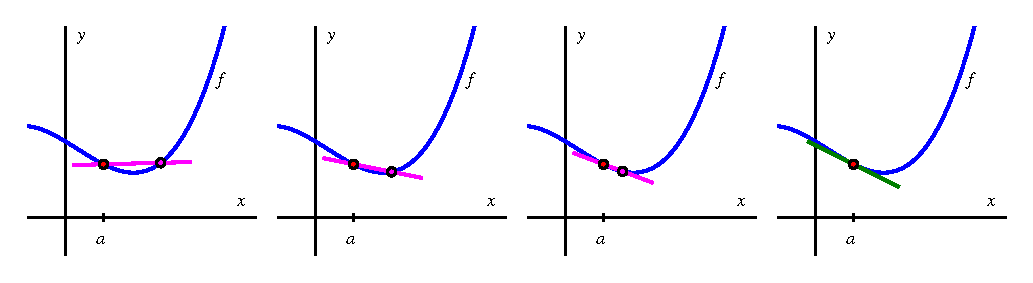
\includegraphics{figures/1_3_SecToTanSeq.eps}}
\end{center}
\caption{A sequence of secant lines approaching the tangent line to $f$ at $(a,f(a))$.} \label{F:1.3.SeqToTanSeq}
\end{figure}

As we will see in subsequent study, the existence of the tangent line at $x = a$ is connected to whether or not the function $f$ looks like a straight line when viewed up close at $(a,f(a))$, which can also be seen in Figure~\ref{F:1.3.SeqToTan}, where we combine the four graphs in Figure~\ref{F:1.3.SeqToTanSeq} into the single one on the left, and then we zoom in on the box centered at $(a,f(a))$, with that view expanded on the right (with two of the secant lines omitted).  Note how the tangent line sits relative to the curve $y = f(x)$ at $(a,f(a))$ and how closely it resembles the curve near $x = a$.

\begin{figure}[h]
\begin{center}
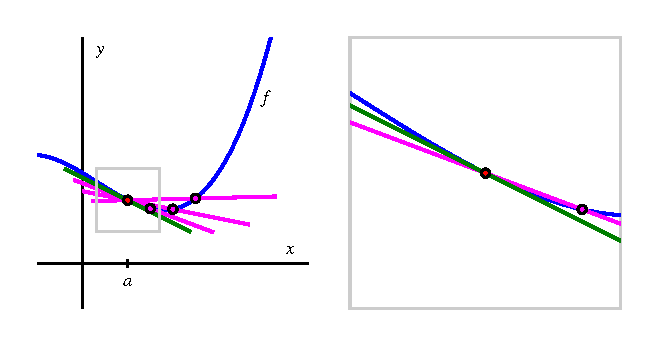
\includegraphics{figures/1_3_SecToTan.eps}
\end{center}
\caption{A sequence of secant lines approaching the tangent line to $f$ at $(a,f(a))$.  At right, we zoom in on the point $(a,f(a))$.  The slope of the tangent line (in green) to $f$ at $(a,f(a))$ is given by $f'(a)$.} \label{F:1.3.SeqToTan}
\end{figure}

At this time, it is most important to note that $f'(a)$, the instantaneous rate of change of $f$ with respect to $x$ at $x = a$, also measures the slope of the tangent line\index{tangent line!slope} to the curve $y = f(x)$ at $(a,f(a))$.  The following example demonstrates several key ideas involving the derivative of a function.

\begin{example}
For the function given by $f(x) = x - x^2$, use the limit definition of the derivative to compute $f'(2)$.  In addition, discuss the meaning of this value and draw a labeled graph that supports your explanation. 
\end{example}
From the limit definition, we know that
$$f'(2) = \lim_{h \to 0} \frac{f(2+h)-f(2)}{h}.$$
Now we use the rule for $f$, and observe that $f(2) = 2 - 2^2 = -2$ and $f(2+h) = (2+h) - (2+h)^2.$  Substituting these values into the limit definition, we have that
$$f'(2) = \lim_{h \to 0} \frac{(2+h) - (2+h)^2 -  (-2)}{h}.$$
Observe that with $h$ in the denominator and our desire to let $h \to 0$, we have to wait to take the limit (that is, we wait to actually let $h$ approach 0).  Thus, we do additional algebra.  Expanding and distributing in the numerator,
$$f'(2) = \lim_{h \to 0} \frac{2+h - 4 - 4h - h^2 + 2}{h}.$$
Combining like terms, we have
$$f'(2) = \lim_{h \to 0} \frac{ -3h - h^2}{h}.$$
Next, we observe that there is a common factor of $h$ in both the numerator and denominator, which allows us to simplify and find that
$$f'(2) = \lim_{h \to 0} (-3-h).$$
Finally, we are able to take the limit as $h \to 0$, and thus conclude that $f'(2) = -3$.

Now, we know that $f'(2)$ represents the slope of the tangent line to the curve $y = x - x^2$ at the point $(2,-2)$; $f'(2)$ is also the instantaneous rate of change of $f$ at the point $(2,-2)$.  Graphing both the function and the line through $(2,-2)$ with slope $m = f'(2) = -3$, we indeed see that by calculating the derivative, we have found the slope of the tangent line at this point, as shown in Figure~\ref{F:1.3.Ex1}.

\begin{figure} \label{F:1.3.Ex1}
\begin{center}
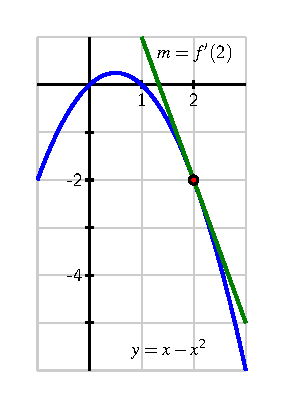
\includegraphics{figures/1_3_Ex1.eps}
\end{center}
\caption{The tangent line to $y = x - x^2$ at the point $(2,-2)$.}
\end{figure}

\begin{center}\underline{}\end{center}

The following activities will help you explore a variety of key ideas related to derivatives.



\begin{activity} \label{A:1.3.1}
Consider the function $f$ whose formula is $\displaystyle f(x) = 3 - 2x$.
\begin{enumerate}
	\item What familiar type of function is $f$?  What can you say about the slope of $f$ at every value of $x$?
	\item Compute the average rate of change of $f$ on the intervals $[1,4]$, $[3,7]$, and $[5,5+h]$; simplify each result as much as possible.  What do you notice about these quantities?
	\item Use the limit definition of the derivative to compute the exact instantaneous rate of change of $f$ with respect to $x$ at the value $a = 1$.  That is, compute $f'(1)$ using the limit definition.  Show your work.  Is your result surprising?
	\item Without doing any additional computations, what are the values of $f'(2)$, $f'(\pi)$, and $f'(-\sqrt{2})$?  Why?
\end{enumerate}
\end{activity}
\begin{hint}[smallhint]
\begin{enumerate}
	\item If $f(x) = 3x^2 + 2x - 4$, we say ``$f$ is quadratic.''  If $f(x) = 5 e^{2x-1}$, we say ``$f$ is exponential.''  What do we say about $f(x) = 3-2x$.  
	\item Remember that to compute the average rate of change of $f$ on $[a,b]$, we calculate $\frac{f(b)-f(a)}{b-a}$.
	\item Observe that $f(1+h) = 3 - 2(1+h) = 3 - 2 - 2h = 1 - 2h$.
	\item Think about the how the graph of $f$ appears.  What is the same at every point?
\end{enumerate}
\end{hint}
\begin{hint}[bighint]
\begin{enumerate}
	\item Observe that the function $f$ is of the form $f(x) = mx + b$.
	\item To compute the average rate of change of $f$ on $[1,4]$, we calculate $\frac{f(4)-f(1)}{4-1}$.
	\item Note that $f(1+h) - f(1) = (3 - 2(1+h)) - (3-2) = 3 - 2 - 2h - 1 = -2h$.
	\item Remember that $f'(a)$ represents the slope of the function $f$ at the value $a$.
\end{enumerate}
\end{hint}
\begin{solution}
\begin{enumerate}
	\item Because $f(x) = 3 - 2x$ is of the form $f(x) = mx + b$, we call $f$ a \emph{linear} function.
	\item The average rate of change on $[1,4]$ is $\frac{f(4)-f(1)}{4-1} = \frac{-5 - 1}{3} = -2$.  Similar calculations show the average rate of change on $[3,7]$ is also $-2$.  On $[5,5+h]$, observe that 
	$$\frac{f(5+h)-f(5)}{h} = \frac{3-2(5+h) - (3-10)}{h} = \frac{3 - 10 - 2h + 7}{h} = \frac{-2h}{h} = -2.$$
	\item Using the limit definition of the derivative, we find that
	\begin{eqnarray*}
		f'(1) & = & \lim_{h \to 0} \frac{f(1+h) - f(1)}{h} \\
			& = & \lim_{h \to 0} \frac{(3 - 2(1+h)) - (3-2)}{h} \\
			& = & \lim_{h \to 0} \frac{3 - 2 - 2h - 1}{h} \\
			& = & \lim_{h \to 0} \frac{-2h}{h} \\
			& = & \lim_{h \to 0} -2 \\
			& = & -2.
	\end{eqnarray*}
\end{enumerate}
\end{solution}

\begin{activity}  \label{A:1.3.2}
A water balloon is tossed vertically in the air from a window.  The balloon's height in feet at time $t$ in seconds after being launched is given by $s(t) = -16t^2 + 16t + 32$. Use this function to respond to each of the following questions.
\begin{enumerate}
	\item Sketch an accurate, labeled graph of $s$ on the axes provided in Figure~\ref{F:1.3.Act2}.  You should be able to do this without using computing technology.
	\begin{figure}[h]
	\begin{center}	
	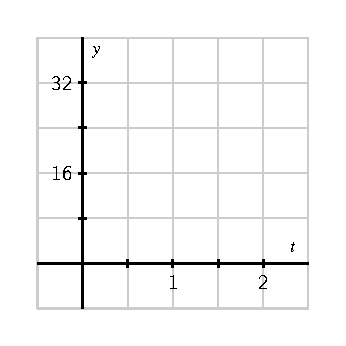
\includegraphics{figures/1_3_Act2.eps}
	\caption{Axes for plotting $y = s(t)$ in Activity~\ref{A:1.3.2}.} \label{F:1.3.Act2}
	\end{center}
	\end{figure}
		
	\item Compute the average rate of change of $s$ on the time interval $[1,2]$.  Include units on your answer and write one sentence to explain the meaning of the value you found.  
	\item Use the limit definition to compute the instantaneous rate of change of $s$ with respect to time, $t$, at the instant $a = 1$.  Show your work using proper notation, include units on your answer, and write one sentence to explain the meaning of the value you found.
	\item On your graph in (a), sketch two lines:  one whose slope represents the average rate of change of $s$ on $[1,2]$, the other whose slope represents the instantaneous rate of change of $s$ at the instant $a=1$.  Label each line clearly.
	\item For what values of $a$ do you expect $s'(a)$ to be positive?  Why?  Answer the same questions when ``positive'' is replaced by ``negative'' and  ``zero.'' 
\end{enumerate}
\end{activity}
\begin{hint}[smallhint]
\begin{enumerate}
	\item Observe that $(t^2 - t - 2) = (t-2)(t+1)$ and that $s(t)$ has its vertex at $t = \frac{1}{2}$.
	\item Recall the formula for average rate of change.
	\item Note that $s(1+h) = -16(1+h)^2 + 16(1+h) + 32$.
	\item Think about a secant line and a tangent line.
	\item A line with positive slope is one that is rising; a line with negative slope is one that is falling.
\end{enumerate}
\end{hint}
\begin{hint}[bighint]
\begin{enumerate}
	\item Show that the quadratic function has $t$-intercepts at $(2,0)$ and $(-1,0)$; $s$-intercept $(0,32)$; and vertex at the point where $t = \frac{1}{2}$.
	\item Compute $\frac{s(2)-s(1)}{2-1}$.
	\item Observe that $s(1+h) - s(1) = (-16(1+h)^2 + 16(1+h) + 32) - (-16(1)^2 + 16(1) + 32) = -16 - 32h - 16h^2 + 16 + 16h + 32 - 32$ and combine like terms carefully.
	\item Consider the line through $(1,s(1))$ and $(2,s(2))$, as well as the line through $(1,s(1))$ with slope $s'(1)$.
	\item Observe that whenever the ball is rising, it's position function is rising, and thus the slope of its tangent line at any such point will be positive.
\end{enumerate}
\end{hint}
\begin{solution}
\begin{enumerate}
	\item Since $s(t) = -16t^2 + 16t + 32 = -16(t^2 - t - 2) = -16(t-2)(t+1)$, $s$ has $t$-intercepts at $(2,0)$ and $(-1,0)$; the $s$-intercept is clearly $(0,32)$; and the vertex is $(\frac{1}{2},36)$.
	\item Observe that $\frac{s(2)-s(1)}{2-1} = \frac{0 - 32}{1} = -32$ feet per second.  This value represents the average rate at which the ball is falling over the time interval from $t = 1$ to $t = 2$.
	\item We compute $s'(1)$ as follows:
	\begin{eqnarray*}
		s'(1) & = & \lim_{h \to 0} \frac{s(1+h)-s(1)}{h} \\
		       & = & \lim_{h \to 0} \frac{(-16(1+h)^2 + 16(1+h) + 32) - (-16(1)^2 + 16(1) + 32)}{h} \\
		       & = & \lim_{h \to 0} \frac{-16 - 32h - 16h^2 + 16 + 16h + 32 - 32}{h} \\
		       & = & \lim_{h \to 0} \frac{-16h - 16h^2}{h} \\
		       & = & \lim_{h \to 0} (-16-16h) \\
		       & = & -16.
	\end{eqnarray*}  
	\item We plot and label the secant line through $(1,s(1))$ and $(2,s(2))$, as well as the tangent line through $(1,s(1))$ with slope $s'(1)$.

	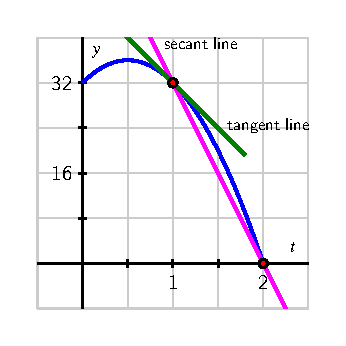
\includegraphics{figures/1_3_Act2Soln.eps}
	
	\item Observe that whenever the ball is rising, it's position function is rising, and thus the slope of its tangent line at any such point will be positive. This means that we should find $s'(a)$ to be positive whenever $0 \le a < \frac{1}{2}$, and similarly $s'(a)$ to be negative whenever $\frac{1}{2} < a < 2$ (which is when the ball is falling).  At the instant $a = \frac{1}{2}$, the ball is at its vertex and is neither rising nor falling, and at that point, $s'(\frac{1}{2}) = 0.$
\end{enumerate}
\end{solution}

\begin{activity}  \label{A:1.3.3}
A rapidly growing city in Arizona has its population $P$ at time $t$, where $t$ is the number of decades after the year 2010, modeled by the formula $P(t) = 25000 e^{t/5}$.  Use this function to respond to the following questions.
\begin{enumerate}
	\item Sketch an accurate graph of $P$ for $t = 0$ to $t = 5$ on the axes provided in Figure~\ref{F:1.3.Act3}.  Label the scale on the axes carefully.
	\begin{figure}[h]
	\begin{center}
	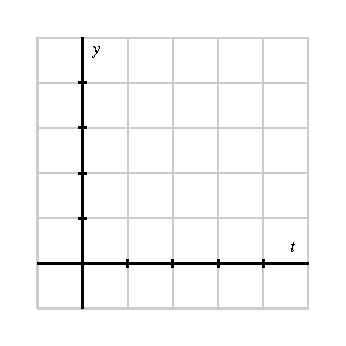
\includegraphics{figures/1_3_Act3.eps} 
	\caption{Axes for plotting $y = P(t)$ in Activity~\ref{A:1.3.3}.} \label{F:1.3.Act3}
	\end{center}
	\end{figure}
	
	\item Compute the average rate of change of $P$ between 2030 and 2050.  Include units on your answer and write one sentence to explain the meaning (in everyday language) of the value you found.
	\item Use the limit definition to write an expression for the instantaneous rate of change of $P$ with respect to time, $t$, at the instant $a = 2$.  Explain why this limit is difficult to evaluate exactly.  
	\item Estimate the limit in (c) for the instantaneous rate of change of $P$ at the instant $a = 2$ by using several small $h$ values.  Once you have determined an accurate estimate of $P'(2)$, include units on your answer, and write one sentence (using everyday language) to explain the meaning of the value you found.
	\item On your graph above, sketch two lines:  one whose slope represents the average rate of change of $P$ on $[2,4]$, the other whose slope represents the instantaneous rate of change of $P$ at the instant $a=2$.
	\item In a carefully-worded sentence, describe the behavior of $P'(a)$ as $a$ increases in value.  What does this reflect about the behavior of the given function $P$?
\end{enumerate}
\end{activity}
\begin{hint}[smallhint]
\begin{enumerate}
	\item $P(t)$ is the standard exponential function, scaled by $25000$.
	\item Use the formula for the average rate of change of a function.
	\item Because of the exponential nature of $P(t)$, we're not able to simplify $\frac{P(2+h)-P(2)}{h}$ in a way that removes $h$ from the denominator.  
	\item Try using $h = 0.001, 0.0001, 0.00001$ and $h = -0.001, -0.0001, -0.00001$.  Be careful not to round or use computing precision that is too limited.  
	\item For the first line, think about the points $(2,P(2))$ and $(4,P(4))$.
	\item Visualize the slope of the tangent line and how it changes as a point moves along the curve.
\end{enumerate}
\end{hint}
\begin{hint}[bighint]
\begin{enumerate}
	\item $P(t)$ is the standard exponential function, scaled by $25000$.
	\item Remember that $AV_{[2,4]} = \frac{P(4)-P(2)}{4-2}$, and that the units on $P$ are people, while $t$ is the number of decades after 2010. 
	\item Note that
	$$P'(2) = \lim_{h \to 0} \frac{P(2+h)-P(2)}{h} = \lim_{h \to 0} \frac{25000 e^{2+h}-25000e^2}{h}.$$  
	\item Try using $h = 0.001, 0.0001, 0.00001$ and $h = -0.001, -0.0001, -0.00001$.  Be careful not to round or use computing precision that is too limited.  Think about how using the two values of $h$ nearest 0 together could give you the most accurate result.
	\item For the first line, think about the points $(2,P(2))$ and $(4,P(4))$.  For the second, try the line through $(2,P(2))$ with slope $P'(2)$.
	\item Visualize the slope of the tangent line and how it changes as a point moves along the curve.  Does the slope of the tangent line increase, decrease, or stay the same as the point of tangency moves along the curve from right to left?
\end{enumerate}
\end{hint}
\begin{solution}
\begin{enumerate}
	\item 	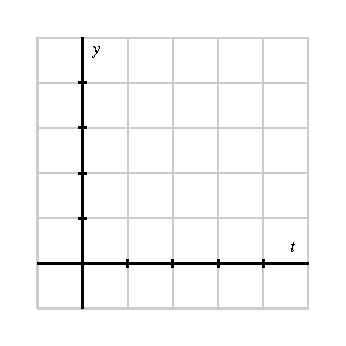
\includegraphics{figures/1_3_Act3.eps}
	\item $AV_{[2,4]} = \frac{P(4)-P(2)}{4-2} = \frac{25000e^{4/5} - 25000e^{2/5}}{2} \approx 9171$ people per decade is expected to be the average rate of change of the city's population over the two decades from 2030 to 2050.
	\item Note that
	\begin{eqnarray*} P'(2) & = & \lim_{h \to 0} \frac{P(2+h)-P(2)}{h} = \lim_{h \to 0} \frac{25000 e^{(2+h)/5}-25000e^{2/5}}{h} \\
	                                 & = &  \lim_{h \to 0} \frac{25000 e^{2/5} e^{h/5} -25000e^{2/5}}{h} =  \lim_{h \to 0} 25000e^{2/5}\left( \frac{e^{h/5} - 1}{h}\right)	\end{eqnarray*}
Because there is no way to remove a factor of $h$ from the numerator, we cannot eliminate the $h$ that is making the denominator go to zero, so it appears we need to be content estimating the limit with small values of $h$.
	\item Using $h = 0.00001$, we find $\frac{P(2+0.00001)-P(2)}{0.00001} \approx 7457$; using $h = -0.00001$, we find $\frac{P(2-0.00001)-P(2)}{-0.00001} \approx 7460$.  Averaging these two results, we find that
	$$P'(2) =  \lim_{h \to 0} \frac{P(2+h)-P(2)}{h} \approx 7458.5$$
	which is measured in people per decade.
	\item See the graph provided in (a) above.  The magenta line has slope equal to the average rate of change of $P$ on $[2,4]$, while the green line is the tangent line at $(2,P(2))$ with slope $P'(2)$.
	\item If we consider the point where $t = a$ and let $a$ start at 0 and then increase, it appears that the tangent line's slope at the point $(a,P(a))$ will increase as $a$ increases.
\end{enumerate}
\end{solution}


\begin{authornote}
This is an author note.
\end{authornote}


\begin{summary}
\item The average rate of change of a function $f$ on the interval $[a,b]$ is $\ds \frac{f(b)-f(a)}{b-a}$.  The units on the average rate of change are units of $f$ per unit of $x$, and the numerical value of the average rate of change represents the slope of the secant line between the points $(a,f(a))$ and $(b,f(b))$ on the graph of $y = f(x)$.  If we view the interval as being $[a,a+h]$ instead of $[a,b]$, the meaning is still the same, but the average rate of change is now computed by  $\ds \frac{f(a+h)-f(a)}{h}$.
\item The instantaneous rate of change with respect to $x$ of a function $f$ at a value $x = a$ is denoted $f'(a)$ (read ``the derivative of $f$ evaluated at $a$'' or ``$f$-prime at $a$'') and is defined by the formula
$$f'(a) = \lim_{h \to 0} \frac{f(a+h)-f(a)}{h},$$
provided the limit exists.  Note particularly that the instantaneous rate of change at $x = a$ is the limit of the average rate of change on $[a,a+h]$ as $h \to 0$.
\item Provided the derivative $f'(a)$  exists, its value tells us the instantaneous rate of change of $f$ with respect to $x$ at $x = a$, which geometrically is the slope of the tangent line to the curve $y = f(x)$ at the point $(a,f(a))$.  We even say that $f'(a)$ is the \emph{slope of the curve} $y = f(x)$ at the point $(a,f(a))$.
\item Limits are the link between average rate of change and instantaneous rate of change: they allow us to move from the rate of change over an interval to the rate of change at a single point.
\end{summary}



\begin{exercises}
\begin{enumerate}
\begin{enumerate} 
\item Consider the graph of $y = f(x)$ provided in Figure~\ref{F:1.3.Ez1}.
	\begin{enumerate}
		\item On the graph of $y = f(x)$, sketch and label the following quantities:
		\begin{itemize}
			\item the secant line to $y = f(x)$ on the interval $[-3,-1]$ and the secant line to $y = f(x)$ on the interval $[0,2]$.
			\item the tangent line to $y = f(x)$ at $x = -3$ and the tangent line to $y = f(x)$ at $x = 0$.
		\end{itemize}
\begin{figure}[h]
  \begin{center}
 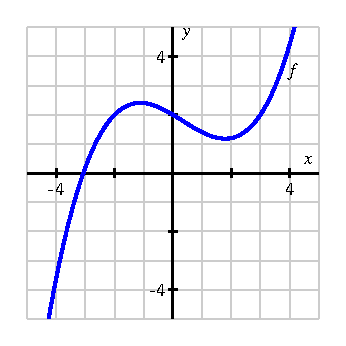
\includegraphics{figures/1_3_Ez1.eps}    \end{center}
   \caption{Plot of $y = f(x)$.} \label{F:1.3.Ez1}
\end{figure}
		\item What is the approximate value of the average rate of change of $f$ on $[-3,-1]$?  On $[0,2]$?  How are these values related to your work in (a)?
		\item What is the approximate value of the instantaneous rate of change of $f$ at $x = -3$?  At $x = 0$?  How are these values related to your work in (a)?

	\end{enumerate}	
	
\begin{solution}
\end{solution}
\item For each of the following prompts, sketch a graph on the provided axes in Figure~\ref{F:1.3.Ez2} of a function that has the stated properties.
  \begin{enumerate}
  	\item $y = f(x)$ such that 
	\begin{itemize}
		\item the average rate of change of $f$ on $[-3,0]$ is $-2$ and the average rate of change of $f$ on $[1,3]$ is 0.5, and
		\item the instantaneous rate of change of $f$ at $x = -1$ is $-1$ and the instantaneous rate of change of $f$ at $x = 2$ is 1. 
	\end{itemize}
	\item $y = g(x)$ such that
	\begin{itemize}
		\item $\frac{g(3)-g(-2)}{5} = 0$ and $\frac{g(1)-g(-1)}{2} = -1$, and
		\item $g'(2) = 1$ and $g'(-1) = 0$
	\end{itemize}
\begin{figure}[h]
  \begin{center}
 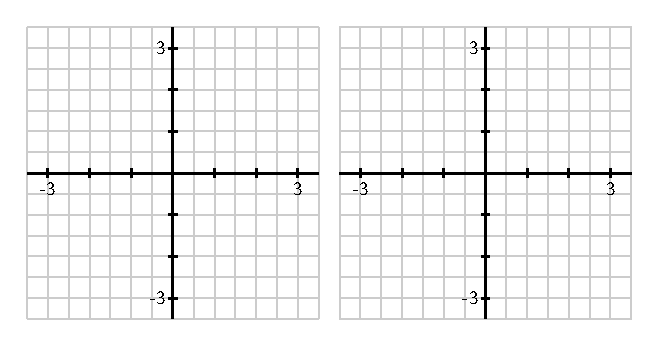
\includegraphics{figures/1_2_Ez3.eps} 
   \end{center}
   \caption{Axes for plotting $y = f(x)$ in (a) and $y = g(x)$ in (b).} \label{F:1.3.Ez2}
\end{figure}
  \end{enumerate}

\item Suppose that the population, $P$, of China (in billions) can be approximated by the function $P(t) = 1.15(1.014)^t$ where $t$ is the number of years since the start of 1993.
   \begin{enumerate}
   	\item According to the model, what was the total change in the population of China between January 1, 1993 and January 1, 2000?  What will be the average rate of change of the population over this time period?  Is this average rate of change greater or less than the instantaneous rate of change of the population on January 1, 2000?  Explain and justify, being sure to include proper units on all your answers.
	\item According to the model, what is the average rate of change of the population of China in the ten-year period starting on January 1, 2012?
	\item Write an expression involving limits that, if evaluated, would give the exact instantaneous rate of change of the population on today's date.  Then estimate the value of this limit (discuss how you chose to do so) and explain the meaning (including units) of the value you have found.
	\item Find an equation for the tangent line to the function $y = P(t)$ at the point where the $t$-value is given by today's date.  
   \end{enumerate}

\item The goal of this problem is to compute the value of the derivative at a point for several different functions, where for each one we do so in three different ways, and then to compare the results to see that each produces the same value.

For each of the following functions, use the limit definition of the derivative to compute the value of $f'(a)$ using three different approaches:  strive to use the algebraic approach first (to compute the limit exactly), then test your result using numerical evidence (with small values of $h$), and finally plot the graph of $y = f(x)$ near $(a,f(a))$ along with the appropriate tangent line to estimate the value of $f'(a)$ visually.  Compare your findings among all three approaches; if you are unable to complete the algebraic approach, still work numerically and graphically.

	\begin{enumerate}
		\item $f(x) = x^2 - 3x$, $a = 2$
		\item $f(x) = \frac{1}{x}$, $a = 1$
		\item $f(x) = \sqrt{x}$, $a = 1$
		\item $f(x) = 2 - |x-1|$, $a = 1$
		\item $f(x) = \sin(x)$, $a = \frac{\pi}{2}$
	\end{enumerate}

\end{enumerate}
\end{enumerate}
\end{exercises} 

\clearpage
\section{The derivative function} \label{S:1.4.DerivativeFxn}

\vspace{-14 pt}

In this section, we strive to understand the ideas generated by the following important questions:
\begin{objectives}
\begin{itemize}
\item How does the limit definition of the derivative of a function $f$ lead to an entirely new (but related) function $f'$?
\item What is the difference between writing $f'(a)$ and $f'(x)$?
\item How is the graph of the derivative function $f'(x)$ connected to the graph of $f(x)$?
\item What are some examples of functions $f$ for which $f'$ is not defined at one or more points?
\end{itemize}\end{objectives} 

\subsection*{Introduction}

Given a function $y = f(x)$, we now know that if we are interested in the instantaneous rate of change of the function at $x = a$, or equivalently the slope of the tangent line to $y = f(x)$ at $x = a$, we can compute the value $f'(a)$.  In all of our examples to date, we have arbitrarily identified a particular value of $a$ as our point of interest: $a = 1$, $a = 3$, etc.  But it is not hard to imagine that we will often be interested in the derivative value for more than just one $a$-value, and possibly for many of them.  In this section, we explore how we can move from computing simply $f'(1)$ or $f'(3)$ to working more generally with $f'(a)$, and indeed $f'(x)$.  Said differently, we will work toward understanding how the so-called process of ``taking the derivative'' generates a new function that is derived from the original function $y = f(x)$.  The following preview activity starts us down this path.

\begin{previewactivity} \label{PA:1.4}
Consider the function $f(x) = 4x - x^2$.
\begin{enumerate}
	\item Use the limit definition to compute the following derivative values:  $f'(0)$, $f'(1)$, $f'(2)$, and $f'(3)$.
	\item Observe that the work to find $f'(a)$ is the same, regardless of the value of $a$.  Based on your work in (a), what do you conjecture is the value of $f'(4)$?  How about $f'(5)$?  (Note: you should \emph{not} use the limit definition of the derivative to find either value.)
	\item Conjecture a formula for $f'(a)$ that depends only on the value $a$.  That is, in the same way that we have a formula for $f(x)$ (recall $f(x) = 4x - x^2$), see if you can use your work above to guess a formula for $f'(a)$ in terms of $a$.
\end{enumerate}
\end{previewactivity}

\subsection*{How the derivative is itself a function}

In your work in Preview Activity~\ref{PA:1.4} with $f(x) = 4x - x^2$, you may have found several patterns.  One comes from observing that $f'(0) = 4$, $f'(1) = 2$, $f'(2) = 0$, and $f'(3) = -2$.  That sequence of values leads us naturally to conjecture that $f'(4) = -4$ and $f'(5) = -6.$  Even more than these individual numbers, if we consider the role of $0$, $1$, $2$, and $3$ in the process of computing the value of the derivative through the limit definition, we observe that the particular number has very little effect on our work.  To see this more clearly, we compute $f'(a)$, where $a$ represents a number to be named later.  Following the now standard process of using the limit definition of the derivative, 
\begin{eqnarray*}
	f'(a) & = & \lim_{h \to 0} \frac{f(a + h) - f(a)}{h} \\
		  & = & \lim_{h \to 0} \frac{4(a + h) - (a + h)^2 - (4a-a^2)}{h} \\
		  & = & \lim_{h \to 0} \frac{4a + 4h - a^2 - 2ha - h^2 - 4a+a^2}{h} \\
		   & = & \lim_{h \to 0} \frac{4h - 2ha - h^2}{h} \\
		   & = & \lim_{h \to 0} \frac{h(4 - 2a - h)}{h} \\
		   & = & \lim_{h \to 0} (4 - 2a - h).
\end{eqnarray*}
Here we observe that neither $4$ nor $2a$ depend on the value of $h$, so as $h \to 0$, $(4 - 2a - h) \to (4 - 2a)$.  Thus, $f'(a) = 4 - 2a$.

This observation is consistent with the specific values we found above:  e.g., $f'(3) = 4 - 2(3) = -2$.  And indeed, our work with $a$ confirms that while the particular value of $a$ at which we evaluate the derivative affects the value of the derivative, that value has almost no bearing on the process of computing the derivative.   We note further that the letter being used is immaterial:  whether we call it $a$, $x$, or anything else, the derivative at a given value is simply given by ``4 minus 2 times the value.''  We choose to use $x$ for consistency with the original function given by $y = f(x)$, as well as for the purpose of graphing the derivative function, and thus we have found that for the function $f(x) = 4x - x^2$, it follows that $f'(x) = 4 - 2x.$

Because the value of the derivative function is so closely linked to the graphical behavior of the original function, it makes sense to look at both of these functions plotted on the same domain.  
\begin{figure}[h]
\begin{center}
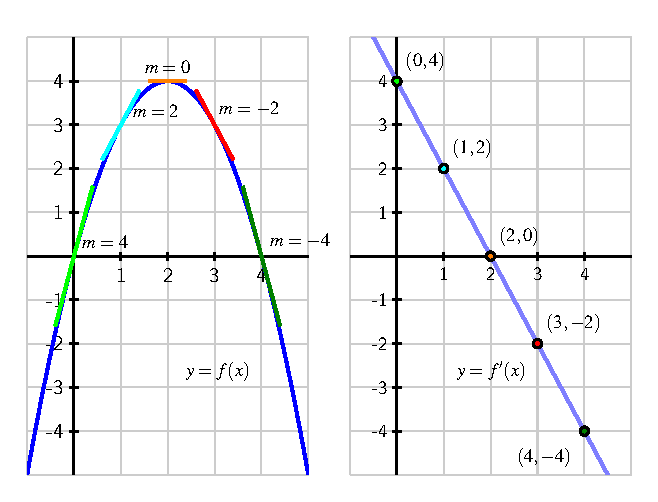
\includegraphics{figures/1_4_ffprimeplot.eps}
\caption{The graphs of $f(x) = 4x - x^2$ (at left) and $f'(x) = 4 - 2x$ (at right).  Slopes on the graph of $f$ correspond to heights on the graph of $f'$.} \label{F:1.4.ffprime}
\end{center}
\end{figure}
In Figure~\ref{F:1.4.ffprime}, on the left we show a plot of $f(x) = 4x - x^2$ together with a selection of tangent lines at the points we've considered above.  On the right, we show a plot of $f'(x) = 4 - 2x$ with emphasis on the heights of the derivative graph at the same selection of points.  Notice the connection between colors in the left and right graph:  the green tangent line on the original graph is tied to the green point on the right graph in the following way:  \emph{the slope of the tangent line} at a point on the lefthand graph is the same as the \emph{height} at the corresponding point on the righthand graph.  That is, at each respective value of $x$, the slope of the tangent line to the original function at that $x$-value is the same as the height of the derivative function at that $x$-value.  Do note, however, that the units on the vertical axes are different:  in the left graph, the vertical units are simply the output units of $f$.  On the righthand graph of $y = f'(x)$, the units on the vertical axis are units of $f$ per unit of $x$.

Of course, this relationship between the graph of a function $y = f(x)$ and its derivative is a dynamic one.  An excellent way to explore how the graph of $f(x)$ generates the graph of $f'(x)$ is through a java applet.  See, for instance, the applets at \href{http://gvsu.edu/s/5C}{\texttt{http://gvsu.edu/s/5C}} or \href{http://gvsu.edu/s/5D}{\texttt{http://gvsu.edu/s/5D}}, via the sites of Austin and Renault\footnote{David Austin, \href{http://gvsu.edu/s/5r}{\texttt{http://gvsu.edu/s/5r}}; Marc Renault, \href{http://gvsu.edu/s/5p}{\texttt{http://gvsu.edu/s/5p}}.}.

In Section~\ref{S:1.3.DerivativePt} when we first defined the derivative, we wrote the definition in terms of a value $a$ to find $f'(a)$.  As we have seen above, the letter $a$ is merely a placeholder, and it often makes more sense to use $x$ instead.  For the record, here we restate the  definition of the derivative\index{derivative!definition}.
\begin{definition} \label{D:derivativedefnx}
Let $f$ be a function and $x$ a value in the function's domain.  We define the \emph{derivative of $f$ with respect to $x$ at the value $x$}, denoted $f'(x)$, by the formula
$\ds f'(x) = \lim_{h \to 0} \frac{f(x+h)-f(x)}{h},$
provided this limit exists.
\end{definition}

We now may take two different perspectives on thinking about the derivative function:  given a graph of $y = f(x)$, how does this graph lead to the graph of the derivative function $y = f'(x)$?  and given a formula for $y = f(x)$, how does the limit definition of the derivative generate a formula for $y = f'(x)$?  Both of these issues are explored in the following activities. 

\begin{activity} \label{A:1.4.1}
For each given graph of $y = f(x)$, sketch an approximate graph of its derivative function, $y = f'(x)$, on the axes immediately below.  The scale of the grid for the graph of $f$ is $1 \times 1$; assume the horizontal scale of the grid for the graph of $f'$ is identical to that for $f$.  If necessary, adjust and label the vertical scale on the axes for  $f'$.

\begin{center}
\scalebox{0.85}{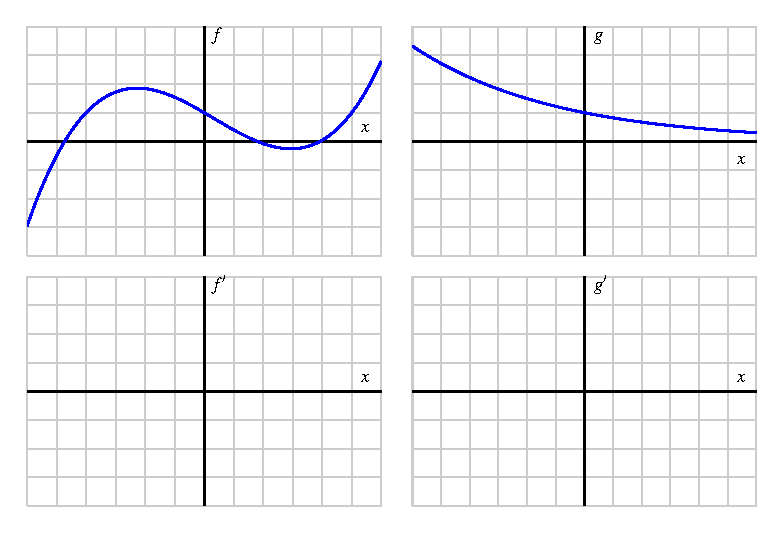
\includegraphics{figures/1_4_Act1a.eps}} 
\scalebox{0.85}{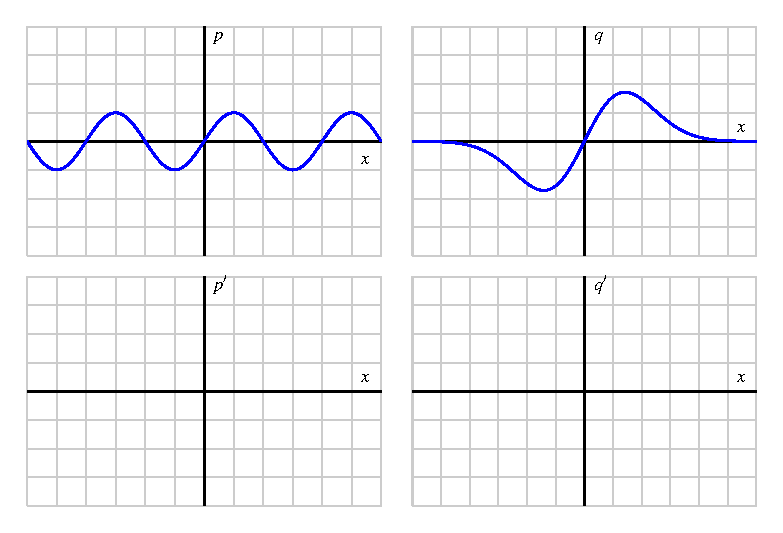
\includegraphics{figures/1_4_Act1b.eps}}

\scalebox{0.85}{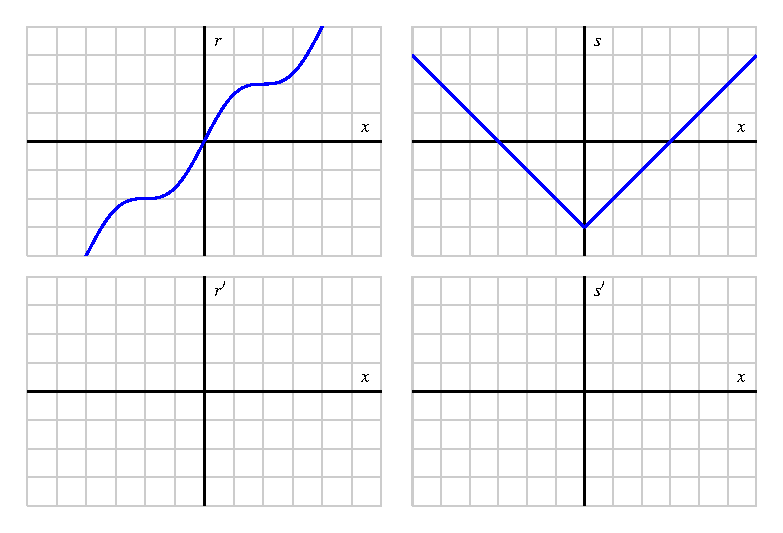
\includegraphics{figures/1_4_Act1c.eps}}
\begin{center}\end{center}
\scalebox{0.85}{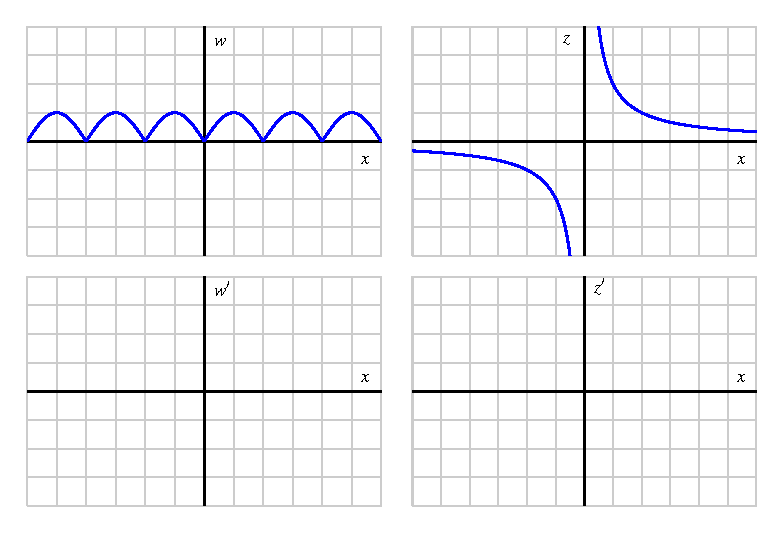
\includegraphics{figures/1_4_Act1d.eps}}
\end{center}

When you are finished with all 8 graphs, write several sentences that describe your overall process for sketching the graph of the derivative function, given the graph the original function.  What are the values of the derivative function that you tend to identify first?  What do you do thereafter?  How do key traits of the graph of the derivative function exemplify properties of the graph of the original function?

\end{activity}
\begin{hint}[smallhint]
Points where the slope of the tangent line is equal to zero are particularly important.  Try finding these points first in your effort to plot $y = f'(x)$ and plotting those zero values on the axes where you'll graph $y = f'(x)$.  
\end{hint}
\begin{hint}[bighint]
Points where the slope of the tangent line is equal to zero are particularly important.  Try finding these points first in your effort to plot $y = f'(x)$ and plotting those zero values on the axes where you'll graph $y = f'(x)$.  After doing so, think carefully as well about the questions: at this point, is $f'(x)$ positive or negative?  is $f'(x)$ big or small.  Use these ideas to help you sketch the derivative graph for the following functions.
\end{hint}
\begin{solution}
\begin{center}
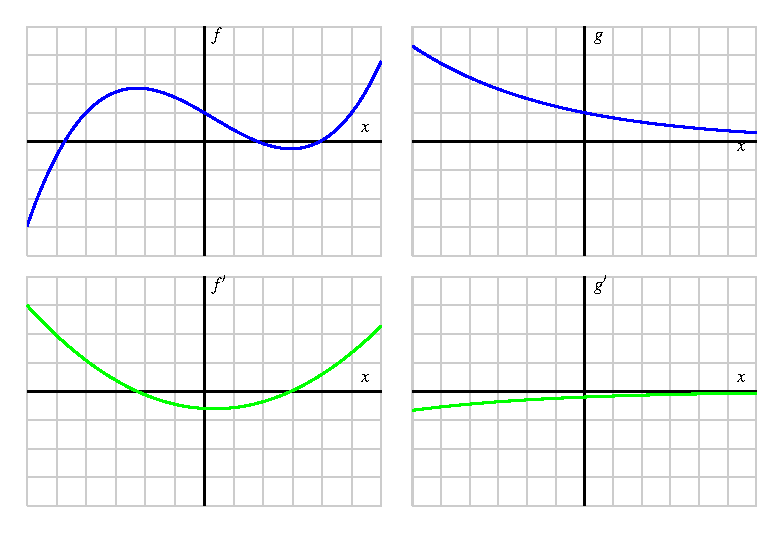
\includegraphics{figures/1_4_Act1aSoln.eps} \\
\underline{}\\
\ \\
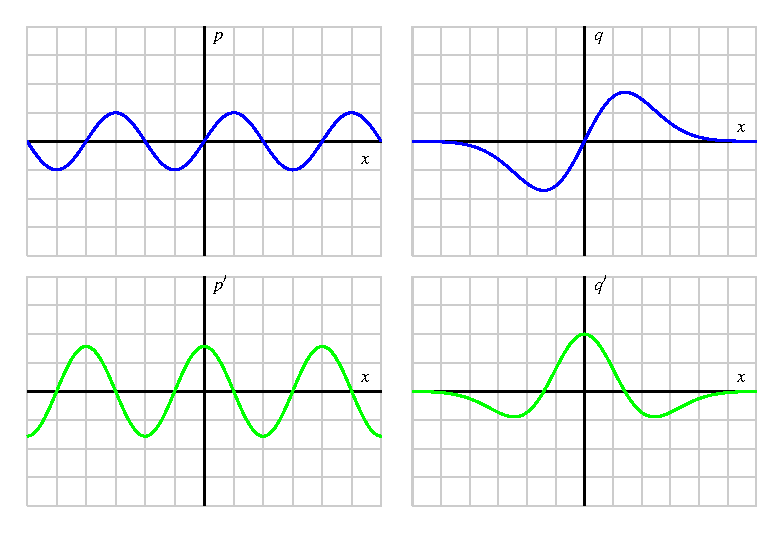
\includegraphics{figures/1_4_Act1bSoln.eps}
\end{center}

\begin{center}
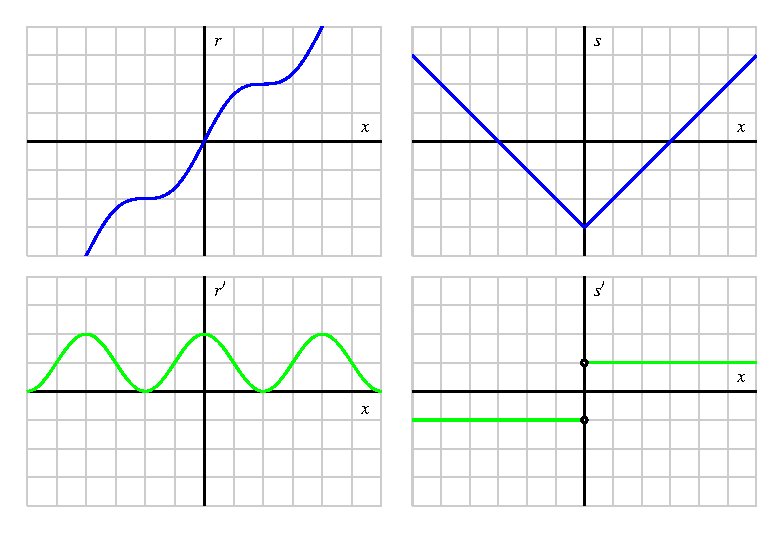
\includegraphics{figures/1_4_Act1cSoln.eps} \\
\underline{}\\
\ \\
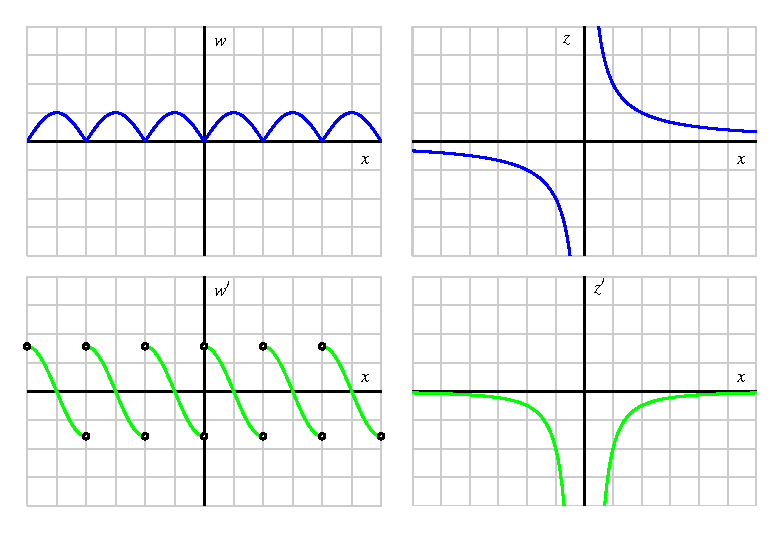
\includegraphics{figures/1_4_Act1dSoln.eps}
\end{center}
\end{solution}

For a dynamic investigation that allows you to experiment with graphing $f'$ when given the graph of $f$, see \href{http://gvsu.edu/s/8y}{\texttt{http://gvsu.edu/s/8y}}.\footnote{Marc Renault, Calculus Applets Using Geogebra.}

Now, recall the opening example of this section:  we began with the function $y = f(x) = 4x - x^2$ and used the limit definition of the derivative to show that $f'(a) = 4 - 2a$, or equivalently that $f'(x) = 4 - 2x$.  We subsequently graphed the functions $f$ and $f'$ as shown in Figure~\ref{F:1.4.ffprime}.  Following Activity~\ref{A:1.4.1}, we now understand that we could have constructed a fairly accurate graph of $f'(x)$ \emph{without} knowing a formula for either $f$ or $f'$.  At the same time, it is ideal to know a formula for the derivative function whenever it is possible to find one.

In the next activity, we further explore the more algebraic approach to finding $f'(x)$:  given a formula for $y = f(x)$, the limit definition of the derivative will be used to develop a formula for $f'(x)$.  

\begin{activity} \label{A:1.4.2}
For each of the listed functions, determine a formula for the derivative function.  For the first two, determine the formula for the derivative by thinking about the nature of the given function and its slope at various points; do not use the limit definition.  For the latter four, use the limit definition.  Pay careful attention to the function names and independent variables.  It is important to be comfortable with using letters other than $f$ and $x$.  For example, given a function $p(z)$, we call its derivative $p'(z)$.
\begin{enumerate}
	\item $f(x) = 1$
	\item $g(t) = t$
	\item $p(z) = z^2$
	\item $q(s) = s^3$
	\item $F(t) = \frac{1}{t}$
	\item $G(y) = \sqrt{y}$
\end{enumerate}

\end{activity}
\begin{hint}[smallhint]
\begin{enumerate}
	\item  What is the slope of the function at every point?
	\item  What is the slope of the function at every point?
	\item  $p(z+h) = (z+h)^2$
	\item  $q(s+h) = (s+h)^3$
	\item  $F(t+h) = \frac{1}{t+h}$
	\item  $G(y+h) = \sqrt{y+h}$
\end{enumerate}
\end{hint}
\begin{hint}[bighint]
\begin{enumerate}
	\item  The function is a horizontal line.
	\item  The function is a line with slope 1.
	\item  $p(z+h) - p(z) = (z+h)^2 - z^2 = z^2 + 2zh + h^2 - z^2$
	\item  $q(s+h) - q(s) = (s+h)^3 - s^3 = s^3 + 3s^2h + 3sh^2 + h^3 - s^3$
	\item  Find a common denominator for $ \frac{1}{t+h} - \frac{1}{t}$.
	\item  Multiply the difference quotient by this form of 1: $\frac{\sqrt{y+h} + \sqrt{y}}{\sqrt{y+h} + \sqrt{y}}.$
\end{enumerate}
\end{hint}
\begin{solution}
\begin{enumerate}
	\item  $f'(x) = 0$ because the slope of the tangent line to the horizontal line given by $f(x) = 1$ is zero at every value of $x$.
	\item  $g'(t) = 1$ because the slope of the tangent line to the line given by $g(t) = t$ is 1 at every value of $t$.
	\item  \begin{eqnarray*}
		p'(z) & = & \lim_{h \to 0} \frac{p(z+h) - p(z)}{h} \\
		       & = & \lim_{h \to 0} \frac{(z+h)^2 - z^2}{h} \\
		       & = & \lim_{h \to 0} \frac{z^2 + 2zh + h^2 - z^2}{h} \\
		       & = & \lim_{h \to 0} \frac{2zh + h^2}{h} \\
		       & = & \lim_{h \to 0} 2z + h \\
		       & = & 2z
		 \end{eqnarray*}
		 
	\item  \begin{eqnarray*}
		q'(s) & = & \lim_{h \to 0} \frac{q(s+h) - q(s)}{h} \\
		       & = & \lim_{h \to 0} \frac{(s+h)^3 - s^3}{h} \\
		       & = & \lim_{h \to 0} \frac{s^3 + 3s^2h + 3sh^2 + h^3 - s^3}{h} \\
		       & = & \lim_{h \to 0} \frac{3s^2h + 3sh^2 + h^2}{h} \\
		       & = & \lim_{h \to 0} 3s^2 + 3sh + h \\
		       & = & 3s^2
		 \end{eqnarray*}
	\item  \begin{eqnarray*}
		F'(t) & = & \lim_{h \to 0} \frac{F(t+h) - F(s)}{h} \\
		       & = & \lim_{h \to 0} \frac{\frac{1}{t+h} - \frac{1}{t}}{h} \\
		       & = & \lim_{h \to 0} \frac{\frac{t - (t+h)}{t(t+h)}}{h} \\
		       & = & \lim_{h \to 0} \frac{-h}{ht(t+h)} \\
		       & = & \lim_{h \to 0} \frac{-1}{t(t+h)} \\
		       & = & \frac{-1}{t^2}
		 \end{eqnarray*}
	\item  \begin{eqnarray*}
		G'(y) & = & \lim_{h \to 0} \frac{G(y+h) - G(y)}{h} \\
		       & = & \lim_{h \to 0} \frac{\sqrt{y+h}-\sqrt{y}}{h} \\
		       & = & \lim_{h \to 0} \frac{\sqrt{y+h}-\sqrt{y}}{h} \cdot \frac{\sqrt{y+h} + \sqrt{y}}{\sqrt{y+h} + \sqrt{y}} \\
		       & = & \lim_{h \to 0} \frac{(y+h)-y}{h(\sqrt{y+h} + \sqrt{y})} \\
		       & = & \lim_{h \to 0} \frac{h}{h(\sqrt{y+h} + \sqrt{y})} \\
		       & = & \lim_{h \to 0} \frac{1}{\sqrt{y+h} + \sqrt{y}} \\
		       & = & \frac{1}{2\sqrt{y}}
		 \end{eqnarray*}		 
\end{enumerate}
\end{solution}

\begin{authornote}
This is an author note.
\end{authornote}


\begin{summary}
\item The limit definition of the derivative, $f'(x) = \lim_{h \to 0} \frac{f(x+h)-f(x)}{h}$, produces a value for each $x$ at which the derivative is defined, and this leads to a new function whose formula is $y = f'(x)$.  Hence we talk both about a given function $f$ and its derivative $f'$.  It is especially important to note that taking the derivative is a process that starts with a given function ($f$) and produces a new, related function ($f'$).
\item There is essentially no difference between writing $f'(a)$ (as we did regularly in Section~\ref{S:1.3.DerivativePt}) and writing $f'(x)$.  In either case, the variable is just a placeholder that is used to define the rule for the derivative function.
\item Given the graph of a function $y = f(x)$, we can sketch an approximate graph of its derivative $y = f'(x)$ by observing that \emph{heights} on the derivative's graph correspond to \emph{slopes} on the original function's graph.
\item In Activity~\ref{A:1.4.1}, we encountered some functions that had sharp corners on their graphs, such as the shifted absolute value function.  At such points, the derivative fails to exist, and we say that $f$ is not differentiable there.  For now, it suffices to understand this as a consequence of the jump that must occur in the derivative function at a sharp corner on the graph of the original function.  
\end{summary}



\begin{exercises}
\begin{enumerate}
\begin{enumerate} 
\item Let $f$ be a function with the following properties:  $f$ is differentiable at every value of $x$ (that is, $f$ has a derivative at every point), $f(-2) = 1$, and $f'(-2) = -2$, $f'(-1) = -1$, $f'(0) = 0$, $f'(1) = 1$, and $f'(2) = 2$.
\begin{enumerate}
	\item On the axes provided at left in Figure~\ref{F:1.4.Ez1}, sketch a possible graph of $y = f(x)$.  Explain why your graph meets the stated criteria.
	\item On the axes at right in Figure~\ref{F:1.4.Ez1}, sketch a possible graph of $y = f'(x)$.  What type of curve does the provided data suggest for the graph of $y = f'(x)$?
	\item Conjecture a formula for the function $y = f(x)$.  Use the limit definition of the derivative to determine the corresponding formula for $y = f'(x)$.  Discuss both graphical and algebraic evidence for whether or not your conjecture is correct.
\end{enumerate}
\begin{figure}[h]
  \begin{center}
 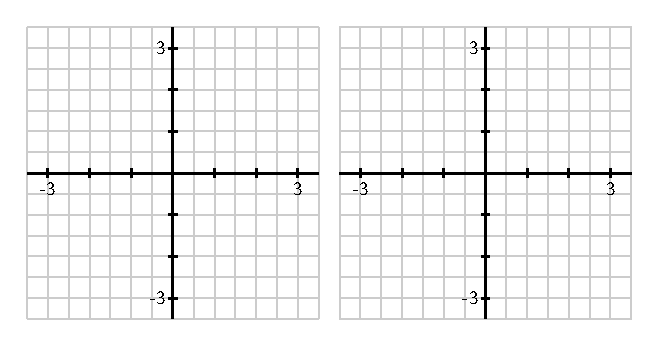
\includegraphics{figures/1_2_Ez3.eps} 
   \end{center}
   \caption{Axes for plotting $y = f(x)$ in (a) and $y = f'(x)$ in (b).} \label{F:1.4.Ez1}
\end{figure}
\begin{solution}
\end{solution}

\item Consider the function $g(x) = x^2 - x + 3$.
\begin{enumerate}
	\item Use the limit definition of the derivative to determine a formula for $g'(x)$.
	\item Use a graphing utility to plot both $y = g(x)$ and your result for $y = g'(x)$; does your formula for $g'(x)$ generate the graph you expected?
	\item Use the limit definition of the derivative to find a formula for $h'(x)$ where $h(x) = 5x^2 - 4x + 12.$
	\item Compare and contrast the formulas for $g'(x)$ and $h'(x)$ you have found.  How do the constants 5, 4, 12, and 3 affect the results?
\end{enumerate}	


\item Let $g$ be a continuous function (that is, one with no jumps or holes in the graph) and suppose that a graph of $y= g'(x)$ is given by the graph  on the right in Figure~\ref{F:1.4.Ez2}.
\begin{figure}[h]
  \begin{center}
 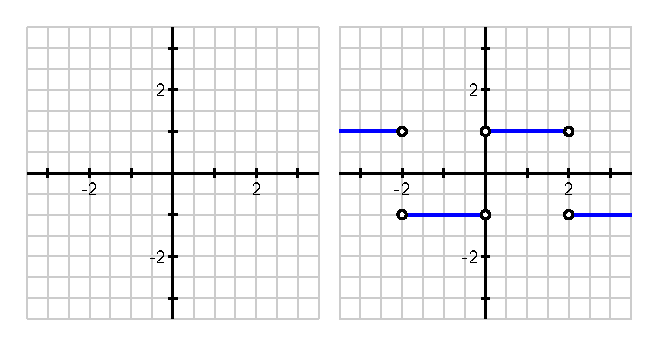
\includegraphics{figures/1_4_Ez2.eps} 
   \end{center}
   \caption{Axes for plotting $y = g(x)$ and, at right, the graph of $y = g'(x)$.} \label{F:1.4.Ez2}
\end{figure}
\begin{enumerate}
	\item Observe that for every value of $x$ that satisfies $0 < x < 2$, the value of $g'(x)$ is constant.  What does this tell you about the behavior of the graph of $y = g(x)$ on this interval?
	\item On what intervals other than $0 < x < 2$ do you expect $y = g(x)$ to be a linear function?  Why?
	\item At which values of $x$ is $g'(x)$ not defined?  What behavior does this lead you to expect to see in the graph of $y=g(x)$?
	\item Suppose that $g(0) = 1$.  On the axes provided at left in  Figure~\ref{F:1.4.Ez2}, sketch an accurate graph of $y = g(x)$.
\end{enumerate}



\item For each graph that provides an original function $y = f(x)$ in Figure~\ref{F:1.4.Ez3a} (on the following page), your task is to sketch an approximate graph of its derivative function, $y = f'(x)$, on the axes immediately below.  View the scale of the grid for the graph of $f$ as being $1 \times 1$, and assume the horizontal scale of the grid for the graph of $f'$ is identical to that for $f$.  If you need to adjust the vertical scale on the axes for the graph of $f'$, you should label that accordingly.

\begin{figure}[h]
  \begin{center}
\scalebox{0.75}{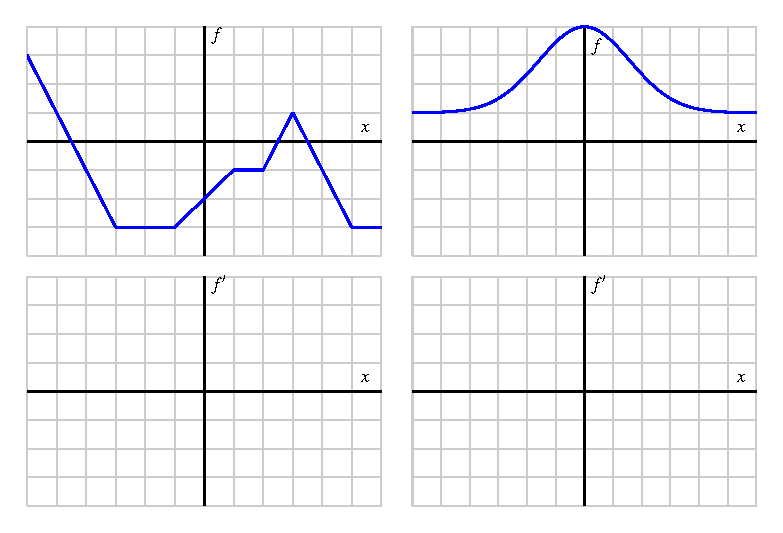
\includegraphics{figures/1_4_Ez3a.eps}} \\
\underline{}\\
\ \\
\scalebox{0.75}{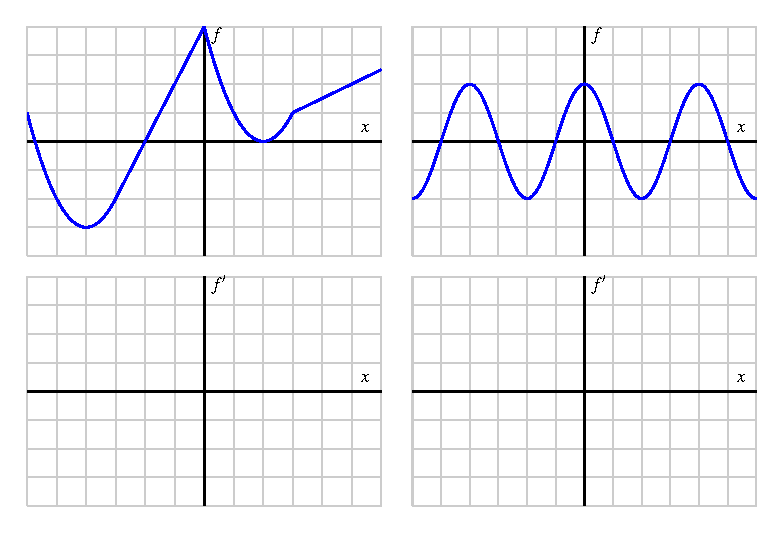
\includegraphics{figures/1_4_Ez3b.eps}}
   \end{center}
   \caption{Graphs of $y = f(x)$ and grids for plotting the corresponding graph of $y = f'(x)$.} \label{F:1.4.Ez3a}
\end{figure}







\end{enumerate}
\end{enumerate}
\end{exercises} 

\clearpage
\section{Interpreting, estimating, and using the derivative} \label{S:1.5.Units}

\vspace{-14 pt}

In this section, we strive to understand the ideas generated by the following important questions:
\begin{objectives}
\begin{itemize}
\item In contexts other than the position of a moving object, what does the derivative of a function measure?
\item What are the units on the derivative function $f'$, and how are they related to the units of the original function $f$?
\item What is a central difference, and how can one be used to estimate the value of the derivative at a point from given function data?
\item Given the value of the derivative of a function at a point, what can we infer about how the value of the function changes nearby?
\end{itemize}\end{objectives} 

\subsection*{Introduction}

An interesting and powerful feature of mathematics is that it can often be thought of both in abstract terms and in applied ones.  For instance, calculus can be developed almost entirely as an abstract collection of ideas that focus on properties of arbitrary functions.  At the same time, calculus can also be very directly connected to our experience of physical reality by considering functions that represent meaningful processes.  We have already seen that for a position function $y = s(t)$, say for a ball being tossed straight up in the air, the ball's velocity at time $t$ is given by $v(t) = s'(t)$, the derivative of the position function.  Further, recall that if $s(t)$ is measured in feet at time $t$, the units on $v(t) = s'(t)$ are feet per second.

In what follows in this section, we investigate several different functions, each with specific physical meaning, and think about how the units on the independent variable, dependent variable, and the derivative function add to our understanding.  To start, we consider the familiar problem of a position function of a moving object.

\begin{previewactivity} \label{PA:1.5}
One of the longest stretches of straight (and flat) road in North America can be found on the Great Plains in the state of North Dakota on state highway 46, which lies just south of the interstate highway I-94 and runs through the town of Gackle.  A car leaves town (at time $t = 0$) and heads east on highway 46; its position in miles from Gackle at time $t$ in minutes is given by the graph of the function in Figure~\ref{F:1.5.PA1}.  Three important points are labeled on the graph; where the curve looks linear, assume that it is indeed a straight line.
\begin{figure}[h]
\begin{center}
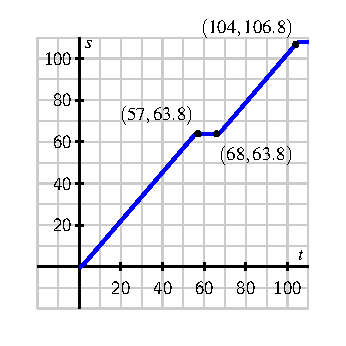
\includegraphics{figures/1_5_PA1.eps}
\caption{The graph of $y = s(t)$, the position of the car along highway 46, which tells its distance in miles from Gackle, ND, at time $t$ in minutes.} \label{F:1.5.PA1}
\end{center}
\end{figure}
\begin{enumerate}
	\item In everyday language, describe the behavior of the car over the provided time interval.  In particular, discuss what is happening on the time intervals $[57,68]$ and $[68,104]$.
	\item Find the slope of the line between the points $(57,63.8)$ and $(104,106.8)$.  What are the units on this slope?  What does the slope represent?
	\item Find the average rate of change of the car's position on the interval $[68,104]$.  Include units on your answer.
	\item Estimate the instantaneous rate of change of the car's position at the moment $t = 80$.  Write a sentence to explain your reasoning and the meaning of this value.
\end{enumerate}
\end{previewactivity}



\subsection*{Units of the derivative function}

As we now know, the derivative of the function $f$ at a fixed value $x$ is given by
$$f'(x) = \ds \lim_{h \to 0} \frac{f(x+h)-f(x)}{h},$$  and this value has several different interpretations.  If we set $x = a$, one meaning of $f'(a)$ is  the slope of the tangent line at the point $(a,f(a))$.

In alternate notation, we also sometimes equivalently write $\frac{df}{dx}$ or $\frac{dy}{dx}$ instead of $f'(x)$, and these notations helps us to further see the units (and thus the meaning) of the derivative as it is viewed as \emph{the instantaneous rate of change of $f$ with respect to $x$}\index{instantaneous rate of change}.  Note that the units on the slope of the secant line, $\frac{f(x+h)-f(x)}{h}$, are ``units of $f$ per unit of $x$.''  Thus, when we take the limit to get $f'(x)$, we get these same units on the derivative $f'(x)$:  units of $f$ per unit of $x$.  Regardless of the function $f$ under consideration (and regardless of the variables being used), it is helpful to remember that the units on the derivative function are ``units of output per unit of input,'' in terms of the input and output of the original function.

For example, say that we have a function $y = P(t)$, where $P$ measures the population of a city (in thousands) at the start of year $t$ (where $t = 0$ corresponds to 2010 AD), and we are told that $P'(2) = 21.37$.  What is the meaning of this value?  Well, since $P$ is measured in thousands and $t$ is measured in years, we can say that the instantaneous rate of change of the city's population with respect to time at the start of 2012 is 21.37 thousand people per year.  We therefore expect that in the coming year, about 21,370 people will be added to the city's population.

\subsection*{Toward more accurate derivative estimates}

It is also helpful to recall, as we first experienced in Section~\ref{S:1.3.DerivativePt}, that when we want to estimate the value of $f'(x)$ at a given $x$, we can use the \emph{difference quotient} \index{difference quotient} $\frac{f(x+h)-f(x)}{h}$ with a relatively small value of $h$.  In doing so, we should use both positive and negative values of $h$ in order to make sure we account for the behavior of the function on both sides of the point of interest.  To that end, we consider the following brief example to demonstrate the notion of a \emph{central difference} and its role in estimating derivatives.

\begin{example} \label{Ex:1.5.1}
Suppose that $y = f(x)$ is a function for which three values are known:  $f(1) = 2.5$, $f(2) = 3.25$, and $f(3) = 3.625$.  Estimate $f'(2)$.
\end{example}
We know that $f'(2) = \lim_{h \to 0} \frac{f(2+h) - f(2)}{h}$.  But since we don't have a graph for $y = f(x)$ nor a formula for the function, we can neither sketch a tangent line nor evaluate the limit exactly.  We can't even use smaller and smaller values of $h$ to estimate the limit.  Instead, we have just two choices:  using $h = -1$ or $h = 1$, depending on which point we pair with $(2,3.25)$.

So, one estimate is
$$f'(2) \approx \frac{f(1)-f(2)}{1-2} = \frac{2.5-3.25}{-1} = 0.75.$$
The other is
$$f'(2) \approx \frac{f(3)-f(2)}{3-2} = \frac{3.625-3.25}{1} = 0.375.$$
Since the first approximation looks only backward from the point $(2,3.25)$ and the second approximation looks only forward from $(2,3.25)$, it makes sense to average these two values in order to account for behavior on both sides of the point of interest.  Doing so, we find that
$$f'(2) \approx \frac{0.75 + 0.375}{2} = 0.5625.$$
\begin{center}\underline{}\end{center}

The intuitive approach to average the two estimates found in Example~\ref{Ex:1.5.1} is in fact the best possible estimate to $f'(2)$ when we have just two function values for $f$ on opposite sides of the point of interest. 
\begin{figure}[h]
\begin{center}
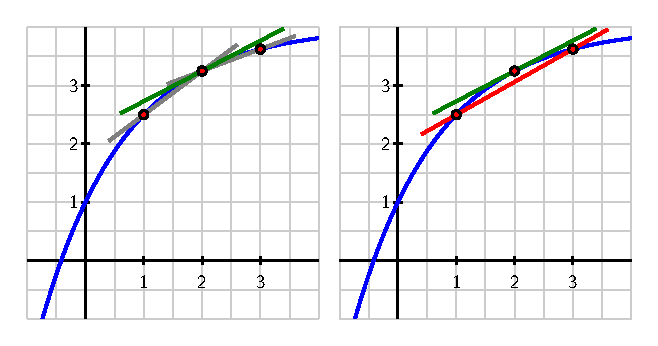
\includegraphics{figures/1_5_Ex1.eps}
\caption{At left, the graph of $y = f(x)$ along with the secant line through $(1,2.5)$ and $(2,3.25)$, the secant line through $(2, 3.25)$ and $(3,3.625)$, as well as the tangent line.  At right, the same graph along with the secant line through $(1,2.5)$ and $(3,3.625)$, plus the tangent line.} \label{F:1.5.Ex1}
\end{center}
\end{figure}
To see why, we think about the diagram in Figure~\ref{F:1.5.Ex1}, which shows
a possible function $y = f(x)$ that satisfies the data given in Example~\ref{Ex:1.5.1}.  On the left, we see the two secant lines with slopes that come from computing the \emph{backward difference} \index{backward difference} $\frac{f(1)-f(2)}{1-2} = 0.75$ and from the \emph{forward difference} \index{forward difference} $\frac{f(3)-f(2)}{3-2} = 0.375.$  Note how the first such line's slope over-estimates the slope of the tangent line at $(2,f(2))$, while the second line's slope underestimates $f'(2)$.  On the right, however, we see the secant line whose slope is given by the \emph{central difference} \index{central difference} $$\frac{f(3)-f(1)}{3-1} = \frac{3.625-2.5}{2} = \frac{1.125}{2} = 0.5625.$$
Note that this central difference has the exact same value as the average of the forward difference and backward difference (and it is straightforward to explain why this always holds), and moreover that the central difference yields a very good approximation to the derivative's value, in part because the secant line that uses both a point before and after the point of tangency yields a line that is closer to being parallel to the tangent line.  

In general, the central difference approximation to the value of the first derivative is given by 
$$f'(a) \approx \frac{f(a+h) - f(a-h)}{2h},$$
and this quantity measures the slope of the secant line to $y = f(x)$ through the points $(a-h, f(a-h))$ and $(a+h, f(a+h))$. Anytime we have symmetric data surrounding a point at which we desire to estimate the derivative, the central difference is an ideal choice for so doing.

The following activities will further explore the meaning of the derivative in several different contexts while also viewing the derivative from graphical, numerical, and algebraic perspectives.

\begin{activity} \label{A:1.5.1}
A potato is placed in an oven, and the potato's temperature $F$ (in degrees Fahrenheit) at various points in time is taken and recorded in the following table. Time $t$ is measured in minutes.

\begin{tabular}{| l || l |}
\hline
$t$ & $F(t)$ \\ \hline \hline
0 & 70\\ \hline
15 & 180.5 \\ \hline
30 & 251 \\ \hline
45 & 296 \\ \hline
60 & 324.5 \\ \hline
75 & 342.8 \\ \hline
90 & 354.5  \\ \hline
\end{tabular}

\begin{enumerate}
	\item Use a central difference to estimate the instantaneous rate of change of the temperature of the potato at $t= 30$. Include units on your answer. 
	\item Use a central difference to estimate the instantaneous rate of change of the temperature of the potato at $t= 60$. Include units on your answer. 
	\item Without doing any calculation, which do you expect to be greater: $F'(75)$ or $F'(90)$?  Why?
	\item Suppose it is given that $F(64) = 330.28$ and $F'(64) = 1.341$.  What are the units on these two quantities?  What do you expect the temperature of the potato to be when $t = 65$?  when $t = 66$?  Why?
	\item Write a couple of careful sentences that describe the behavior of the temperature of the potato on the time interval $[0,90]$, as well as the behavior of the instantaneous rate of change of the temperature of the potato on the same time interval.
\end{enumerate}

\end{activity}
\begin{hint}[smallhint]
\begin{enumerate}
	\item Think about quantities such as $\frac{F(45)-F(30)}{45-30}$.
	\item See the note in (a).
	\item Is $F$ changing faster at $t = 75$ or at $t = 90$?
	\item Remember that the units on $F'$ will be ``degrees Fahrenheit per minute.''
	\item Be careful to distinguish between the temperature, $F$, and the rate of change of temperature, $F'$, in your commentary.
\end{enumerate}
\end{hint}
\begin{hint}[bighint]
\begin{enumerate}
	\item Think about quantities such as $\frac{F(45)-F(30)}{45-30}$ and $\frac{F(15)-F(30)}{15-30}$.
	\item See the note in (a).
	\item What overall trend do you observe in the instantaneous rate of change of $F$, based on the overall trend in temperature $F$?
	\item Remember that the units on $F'$ will be ``degrees Fahrenheit per minute.''
	\item Be careful to distinguish between the temperature, $F$, and the rate of change of temperature, $F'$, in your commentary.
\end{enumerate}
\end{hint}
\begin{solution}
\begin{enumerate}
	\item Using the central difference, we find that 
	$$F'(30) \approx \frac{F(45)-F(15)}{45-15} = \frac{296-180.5}{30} = 3.85$$
	degrees per minute.
	\item Using the central difference, we find that 
	$$F'(60) \approx \frac{F(75)-F(45)}{45-15} = \frac{342.8-296}{30} = 1.56$$
	degrees per minute.
	\item Over each subsequent time interval, we see that the amount of increase in the potato's temperature gets less and less, thus we expect the value of $F'(t)$ to get smaller and smaller as time goes on.  We therefore expect $F'(75) > F'(90)$.
	\item The value $F(64) = 330.28$ is the temperature of the potato in degrees Fahrenheit at time 64, while $F'(64) = 1.341$ measures the instantaneous rate of change of the potato's temperature with respect to time at the instant $t = 64$, and its units are degrees per minute.  Because at time $t = 64$ the potato's temperature is increasing at 1.341 degrees per minute, we expect that at $t = 65$, the temperature will be about 1.341 degrees greater than at $t = 64$, or in other words $F(65) \approx 330.28 + 1.341 = 331.621$.  Similarly, at $t = 66$, two minutes have elapsed from $t = 64$, so we expect an increase of $2 \dot 1.341$ degrees:  $F(66) \approx 330.28 + 2 \cdot 1.341 = 332.962$. 
	\item Throughout the time interval $[0,90]$, the temperature $F$ of the potato is increasing.  But as time goes on, the rate at which the temperature is rising appears to be decreasing.  That is, while the values of $F$ continue to get larger as time progresses, the values of $F'$ are getting smaller (while still remaining positive). We thus might say that ``the temperature of the potato is increasing, but at a decreasing rate.''
\end{enumerate}
\end{solution}



\begin{activity} \label{A:1.5.2}
A company manufactures rope, and the total cost of producing $r$ feet of rope is $C(r)$ dollars.
\begin{enumerate}
	\item What does it mean to say that $C(2000) = 800$?

	\item What are the units of $C'(r)$?

	\item Suppose that $C(2000) = 800$ and $C'(2000) = 0.35$.  Estimate $C(2100)$, and justify your estimate by writing at least one sentence that explains your thinking.

	\item Which of the following statements do you think is true, and why?
	\begin{itemize}
		\item $C'(2000) < C'(3000)$
		\item $C'(2000) = C'(3000)$
		\item $C'(2000) > C'(3000)$
	\end{itemize}

	\item Suppose someone claims that $C'(5000) = -0.1$.  What would the practical meaning of this derivative value tell you about the approximate cost of the next foot of rope?  Is this possible?  Why or why not?  
\end{enumerate}
\end{activity}
\begin{hint}[smallhint]
\begin{enumerate}
	\item The cost of producing 2000 feet of rope is $\ldots$
	\item Remember that the units on any derivative are ``units of output per unit of input.''
	\item How much do you expect $C$ to increase for each additional foot away from 2000?  By how many feet will the input increase to get to 2100?
	\item In manufacturing processes, there is often a decrease in cost per unit as the number of units increases.
	\item Is it possible for the total cost function to be decreasing at some point?
\end{enumerate}
\end{hint}
\begin{hint}[bighint]
\begin{enumerate}
	\item The total cost of producing 2000 feet of rope is $\ldots$
	\item Remember that the units on any derivative are ``units of output per unit of input'' and that the input here is $r$ feet.
	\item Since $C'(2000) = 0.35$ dollars/foot, we expect that for each additional foot of rope, the cost will increase by $0.35$ dollars.
	\item In manufacturing processes, there is often a decrease in cost per unit as the number of units increases.  What does that tell us to expect about the derivative of $C(r)$?
	\item If $C'(5000) = -0.1$, this would tell us that $C(r)$ is a decreasing function at $r = 5000$, which means that the total cost to make $5001$ feet of rope is less than the total cost to make $5000$ feet of rope.  Is this possible?
\end{enumerate}
\end{hint}
\begin{solution}
\begin{enumerate}
	\item $C(2000) = 800$ means that it costs \dollar800 to make 2000 feet of rope.

	\item The units of $C'(r)$ are ``dollars per foot.''

	\item If $C(2000) = 800$ and $C'(2000) = 0.35$, then we know once 2000 feet of rope are produced, the total cost function is increasing at \dollar0.35 per additional foot of rope.  Then, if we manufacture an additional 100 feet of rope, the additional total cost will be approximately 
	$$100 \ \mbox{feet} \cdot 0.35 \ \frac{\mbox{dollars}}{\mbox{foot}} = 35 \ \mbox{dollars}.$$  
	Therefore, we find that $C(2100) \approx C(2000) + 35 = 835,$ or that the cost to make 2100 feet of rope is about \dollar835.

	\item Either $C'(2000) = C'(3000)$ or $C'(2000) > C'(3000)$, since we expect the cost per foot of additional rope to either stay constant or to get smaller as the production volume increases.  Said differently, the instantaneous rate of change of the total cost function should either be constant or decrease due to economy of scale.

	\item It is impossible to have $C'(5000) = -0.1$ and indeed to have any negative derivative value for the total cost function.  The total cost function $C(r)$ can never decrease, because it doesn't make sense for the total cost of producing 5001 feet of rope to be less than the total cost of producing 5000 feet of rope. 
\end{enumerate}
\end{solution}

\begin{activity} \label{A:1.5.3}
Researchers at a major car company have found a function that relates gasoline consumption to speed for a particular model of car.  In particular, they have determined that the consumption $C$, in {\bfseries liters per kilometer}, at a given speed $s$, is given by a function $C = f(s)$, where $s$ is the car's speed in \textbf{kilometers per hour}. 
	\begin{enumerate}
	  \item Data provided by the car company tells us that $f(80) = 0.015$, $f(90) = 0.02$, and $f(100) = 0.027$.  Use this information to estimate the instantaneous rate of change of fuel consumption with respect to speed at $s = 90$.  Be as accurate as possible, use proper notation, and include units on your answer.
	  \item By writing a complete sentence, interpret the meaning (in the context of fuel consumption) of ``$f(80) = 0.015$.'' 
	  \item Write at least one complete sentence that interprets the meaning of the value of $f'(90)$ that you estimated in (a).
	\end{enumerate}
\end{activity}
\begin{hint}[smallhint]
\begin{enumerate}
	\item Try a central difference.
	\item What is happening when the car is traveling at 80 km/hr?
	\item Remember that units on the derivative are ``units of output per unit of input.''
\end{enumerate}
\end{hint}
\begin{hint}[bighint]
\begin{enumerate}
	\item Remember that $f'(a) \approx \frac{f(a+h)-f(a-h)}{2h}$ and use appropriate values of $a$ and $h$.
	\item Complete the following sentence: ``When the car is traveling at 80 kilometers per hour, it is using fuel at a rate of 0.015 $\ldots$''
	\item Remember that units on the derivative are ``units of output per unit of input,'' even when the input and/or output are rates themselves.
\end{enumerate}
\end{hint}
\begin{solution}
\begin{enumerate}
	\item Using a central difference, we have
	$$f'(90) = \frac{f(100) - f(80}{100-80} = \frac{0.027 - 0.015}{20} = \frac{0.012}{20} = 0.0006$$
	which tells us that $f'(90) = 0.0006$ liters per kilometer per kilometer per hour.
	\item When the car is traveling at 80 kilometers per hour, it is using fuel at a rate of 0.015 liters per kilometer.  That is, at the given speed, for each additional kilometer the car travels, it uses an additional 0.015 liters of fuel.
	\item To say that $f'(90) = 0.0006$ liters per kilometer per kilometer per hour means that when the car is traveling at 90 kilometers per hour, its rate of fuel consumption per kilometer is increasing at a rate of 0.0006 liters per kilometer per kilometer per hour.  If we increase our speed from 90 to 91 km/hr, we would expect our rate of fuel consumption to rise by 0.0006 liters for each additional kilometer driven.
\end{enumerate}
\end{solution}

In Section~\ref{S:1.4.DerivativeFxn}, we learned how use to the graph of a given function $f$ to plot the graph of its derivative, $f'$.  It is important to remember that when we do so, not only does the scale on the vertical axis often have to change to accurately represent $f'$, but the units on that axis also differ.  For example, suppose that $P(t) = 400-330e^{-0.03t}$ tells us the temperature in degrees Fahrenheit of a potato in an oven at time $t$ in minutes.  In Figure~\ref{F:1.5.PPprime}, we sketch the graph of $P$ on the left and the graph of $P'$ on the right.  

\begin{figure}[h]
\begin{center}
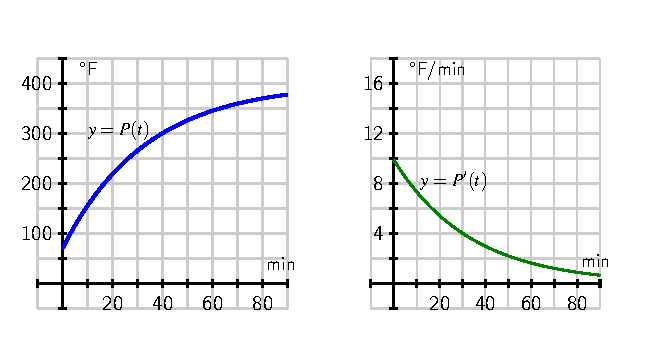
\includegraphics{figures/1_5_PPprimeplot.eps}
\caption{Plot of $P(t) = 400-330e^{-0.03t}$ at left, and its derivative $P'(t)$ at right.}\label{F:1.5.PPprime}
\end{center}
\end{figure}

Note how not only are the vertical scales different in size, but different in units, as the units of $P$ are $^{\circ}$F, while those of $P'$ are $^{\circ}$F/min.  In all cases where we work with functions that have an applied context, it is helpful and instructive to think carefully about units involved and how they further inform the meaning of our computations.

\begin{summary}
\item Regardless of the context of a given function $y=f(x)$, the derivative always measures the instantaneous rate of change of the output variable with respect to the input variable.
\item The units on the derivative function $y = f'(x)$ are units of $f$ per unit of $x$.  Again, this measures how fast the output of the function $f$ changes when the input of the function changes.
\item The central difference approximation to the value of the first derivative is given by 
$$f'(a) \approx \frac{f(a+h) - f(a-h)}{2h},$$
and this quantity measures the slope of the secant line to $y = f(x)$ through the points $(a-h, f(a-h))$ and $(a+h, f(a+h))$.  The central difference generates a good approximation of the derivative's value any time we have symmetric data surrounding a point of interest.
\item Knowing the derivative and function values at a single point enables us to estimate other function values nearby.  If, for example, we know that $f'(7) = 2$, then we know that at $x = 7$, the function $f$ is increasing at an instantaneous rate of 2 units of output for every one unit of input.  Thus, we expect $f(8)$ to be approximately 2 units greater than $f(7)$.  The value is approximate because we don't know that the rate of change stays the same as $x$ changes.
\end{summary}



\begin{exercises}
\begin{enumerate}
\begin{enumerate} 
\item A cup of coffee has its temperature $F$ (in degrees Fahrenheit) at time $t$ given by the function $F(t) = 75 + 110 e^{-0.05t}$, where time is measured in minutes.
	\begin{enumerate}
		\item Use a central difference with $h = 0.01$ to estimate the value of $F'(10)$.
		\item What are the units on the value of $F'(10)$ that you computed in (a)?  What is the practical meaning of the value of $F'(10)$?
		\item Which do you expect to be greater: $F'(10)$ or $F'(20)$?  Why?  
		\item Write a sentence that describes the behavior of the function $y = F'(t)$ on the time interval $0 \le t \le 30$.  How do you think its graph will look?  Why?
	\end{enumerate}
\item The temperature change $T$ (in Fahrenheit degrees), in a patient, that is generated by a dose $q$ (in milliliters), of a drug, is given by the function $T = f(q)$.
\begin{enumerate}
	\item What does it mean to say $f(50) = 0.75$?  Write a complete sentence to explain, using correct units.
	\item A person's sensitivity, $s$, to the drug is defined by the function $s(q) = f'(q)$.  What are the units of sensitivity?
	\item Suppose that $f'(50) = -0.02$.  Write a complete sentence to explain the meaning of this value.  Include in your response the information given in (a).
\end{enumerate}
\begin{solution}
\end{solution}
\item The velocity of a ball that has been tossed vertically in the air is given by $v(t) = 16 - 32t$, where $v$ is measured in feet per second, and $t$ is measured in seconds.  The ball is in the air from $t = 0$ until $t = 2$.
\begin{enumerate}
	\item When is the ball's velocity greatest?
	\item Determine the value of $v'(1)$.  Justify your thinking.
	\item What are the units on the value of $v'(1)$?  What does this value and the corresponding units tell you about the behavior of the ball at time $t = 1$?  
	\item What is the physical meaning of the function $v'(t)$?
\end{enumerate}

\item The value, $V$, of a particular automobile (in dollars) depends on the number of miles, $m$, the car has been driven, according to the function $V = h(m)$.  
\begin{enumerate}
	\item Suppose that $h(40000) = 15500$ and $h(55000) = 13200$.  What is the average rate of change of $h$ on the interval $[40000,55000]$, and what are the units on this value?
	\item In addition to the information given in (a), say that $h(70000) = 11100$.  Determine the best possible estimate of $h'(55000)$ and write one sentence to explain the meaning of your result, including units on your answer.
	\item Which value do you expect to be greater: $h'(30000)$ or $h'(80000)$?  Why?
	\item Write a sentence to describe the long-term behavior of the function $V = h(m)$, plus another sentence to describe the long-term behavior of $h'(m)$.  Provide your discussion in practical terms regarding the value of the car and the rate at which that value is changing.
\end{enumerate}
\end{enumerate}
\end{enumerate}
\end{exercises} 

\clearpage
\section{The second derivative} \label{S:1.6.SecondD}

\vspace{-14 pt}

In this section, we strive to understand the ideas generated by the following important questions:
\begin{objectives}
\begin{itemize}
\item How does the derivative of a function tell us whether the function is increasing or decreasing at a point or on an interval?
\item What can we learn by taking the derivative of the derivative (to achieve the \emph{second} derivative) of a function $f$?
\item What does it mean to say that a function is concave up or concave down?  How are these characteristics connected to certain properties of the derivative of the function?
\item What are the units on the second derivative?  How do they help us understand the rate of change of the rate of change?
\end{itemize}\end{objectives} 

\subsection*{Introduction}

Given a differentiable function $y= f(x)$, we know that its derivative, $y = f'(x)$, is a related function whose output at a value $x=a$ tells us the slope of the tangent line to $y = f(x)$ at the point $(a,f(a))$.  That is, heights on the derivative graph tell us the values of slopes on the original function's graph.  Therefore, the derivative tells us important information about the function $f$.  

\begin{figure}[h]
\begin{center}
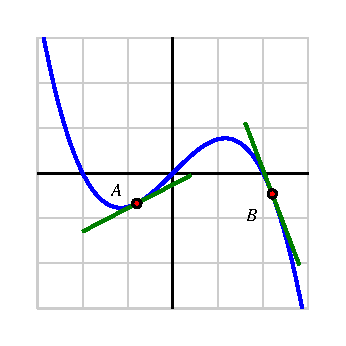
\includegraphics{figures/1_6_Intro.eps}
\caption{Two tangent lines on a graph demonstrate how the slope of the tangent line tells us whether the function is rising or falling, as well as whether it is doing so rapidly or slowly.} \label{F:1.6.Intro}
\end{center}
\end{figure}

At any point where $f'(x)$ is positive, it means that the slope of the tangent line to $f$ is positive, and therefore the function $f$ is increasing (or rising) \index{increasing} at that point.  Similarly, if $f'(a)$ is negative, we know that the graph of $f$ is decreasing \index{decreasing} (or falling) at that point.   

In the next part of our study, we work to understand not only \emph{whether} the function $f$ is increasing or decreasing at a point or on an interval, but also \emph{how} the function $f$ is increasing or decreasing.  Comparing the two tangent lines shown in Figure~\ref{F:1.6.Intro}, we see that at point $A$, the value of $f'(x)$ is positive and relatively close to zero, which coincides with the graph rising slowly.  By contrast, at point $B$, the derivative is negative and relatively large in absolute value, which is tied to the fact that $f$ is decreasing rapidly at $B$.  It also makes sense to not only ask whether the value of the derivative function is positive or negative and whether the derivative is large or small, but also to ask ``how is the derivative changing?''

We also now know that the derivative, $y = f'(x)$, is itself a function.  This means that we can consider taking its derivative -- the derivative of the derivative -- and therefore ask questions like ``what does the derivative of the derivative tell us about how the original function behaves?''  As we have done regularly in our work to date, we start with an investigation of a familiar problem in the context of a moving object.  

\begin{previewactivity} \label{PA:1.6}
The position of a car driving along a straight road at time $t$ in minutes is given by the function $y = s(t)$ that is pictured in Figure~\ref{F:1.6.PA1}.  The car's position function has units measured in thousands of feet.  For instance, the point $(2,4)$ on the graph indicates that after 2 minutes, the car has traveled 4000 feet.
\begin{figure}[h]
\begin{center}
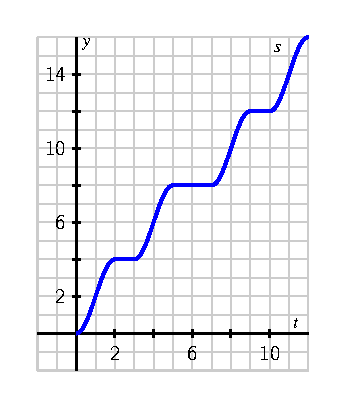
\includegraphics{figures/1_6_PA1.eps}
\caption{The graph of $y = s(t)$, the position of the car (measured in thousands of feet from its starting location) at time $t$ in minutes.} \label{F:1.6.PA1}
\end{center}
\end{figure}
\begin{enumerate}
	\item In everyday language, describe the behavior of the car over the provided time interval.  In particular, you should carefully discuss what is happening on each of the time intervals $[0,1]$, $[1,2]$, $[2,3]$, $[3,4]$, and $[4,5]$, plus provide commentary overall on what the car is doing on the interval $[0,12]$.
	\item On the lefthand axes provided in Figure~\ref{F:1.6.PA1b}, sketch a careful, accurate graph of $y = s'(t)$.
	\item What is the meaning of the function $y = s'(t)$ in the context of the given problem?  What can we say about the car's behavior when $s'(t)$ is positive?  when $s'(t)$ is zero?  when $s'(t)$ is negative?
	\item Rename the function you graphed in (b) to be called $y = v(t)$.  Describe the behavior of $v$ in words, using phrases like ``$v$ is increasing on the interval $\ldots$'' and ``$v$ is constant on the interval $\ldots$.''
	\item Sketch a graph of the function $y = v'(t)$ on the righthand axes provide in Figure~\ref{F:1.6.PA1b}.  Write at least one sentence to explain how the behavior of $v'(t)$ is connected to the graph of $y=v(t)$.
\end{enumerate}
\begin{figure}[h]
\begin{center}
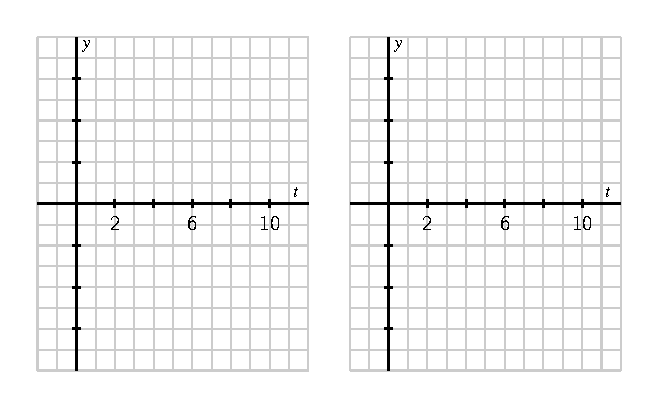
\includegraphics{figures/1_6_PA1b.eps}
\caption{Axes for plotting $y = v(t) = s'(t)$ and $y = v'(t)$.} \label{F:1.6.PA1b}
\end{center}
\end{figure}
\end{previewactivity} 




\subsection*{Increasing, decreasing, or neither}

When we look at the graph of a function, there are features that strike us naturally, and common language can be used to name these features.  In many different settings so far, we have intuitively used the words \emph{increasing} and \emph{decreasing} to describe a function's graph.  Here we connect these terms more formally to a function's behavior on an interval of input values.
\begin{definition}
Given a function $f(x)$ defined on the interval $(a,b)$, we say that \emph{$f$ is increasing on $(a,b)$} provided that for all $x$, $y$ in the interval $(a,b)$, if $x < y$, then $f(x) < f(y)$.  Similarly, we say that \emph{$f$ is decreasing on $(a,b)$} provided that for all $x$, $y$ in the interval $(a,b)$, if $x < y$, then $f(x) > f(y)$.
\end{definition}
Simply put, an increasing function is one that is rising as we move from left to right along the graph, and a decreasing function is one that falls as the value of the input increases.  For a function that has a derivative at a point, we will also talk about whether or not the function is increasing or decreasing \emph{at that point}.  Moreover, the fact of whether or not the function is increasing, decreasing, or neither at a given point depends precisely on the value of the derivative at that point.

\vspace{5pt}
 

Let $f$ be a function that is differentiable at $x = a$.  Then $f$ is increasing at $x = a$ if and only if $f'(a) > 0$ and $f$ is decreasing at $x = a$ if and only if $f'(a) < 0$.  If $f'(a) = 0$, then we say $f$ is neither increasing nor decreasing at $x = a$.
 
\vspace{1pt}

\begin{figure}[h]
\begin{center}
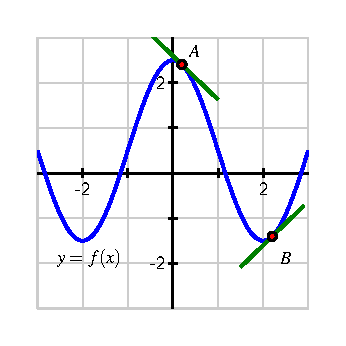
\includegraphics{figures/1_6_Intro2.eps}
\caption{A function that is decreasing at $A$, increasing at $B$, and more generally, decreasing on the intervals $-3 < x < -2$ and $0 < x  < 2$ and increasing on $-2 < x < 0$ and $2 < x < 3$.} \label{F:1.6.Intro2}
\end{center}
\end{figure}

For example, the function pictured in Figure~\ref{F:1.6.Intro2} is increasing at any point at which $f'(x)$ is positive, and hence is increasing on the entire interval $-2 < x < 0$.  Note that at both $x = \pm 2$ and $x = 0$, we say that $f$ is neither increasing nor decreasing, because $f'(x) = 0$ at these values.

\subsection*{The Second Derivative} \index{second derivative}

For any function, we are now accustomed to investigating its behavior by thinking about its derivative.  Given a function $f$, its derivative is a new function, one that is given by the rule
$$f'(x) = \lim_{h \to 0} \frac{f(x+h)-f(x)}{h}.$$
Because $f'$ is itself a function, it is perfectly feasible for us to consider the derivative of the derivative, which is the new function $y = [f'(x)]'$.  We call this resulting function \emph{the second derivative}\index{second derivative} of $y = f(x)$, and denote the second derivative by $y = f''(x)$.
Due to the presence of multiple possible derivatives, we will sometimes call $f'$ ``the first derivative'' of $f$, rather than simply ``the derivative'' of $f$. Formally, the second derivative is defined by the limit definition of the derivative of the first derivative:
$$f''(x) = \lim_{h \to 0} \frac{f'(x+h)-f'(x)}{h}.$$


We note that all of the established meaning of the derivative function still holds, so when we compute $y = f''(x)$, this new function measures slopes of tangent lines to the curve $y = f'(x)$, as well as the instantaneous rate of change of $y = f'(x)$.  In other words, just as the first derivative measures the rate at which the original function changes, the second derivative measures the rate at which the first derivative changes.  This means that the second derivative tracks the instantaneous rate of change of the instantaneous rate of change of $f$.  That is, the second derivative will help us to understand how the rate of change of the original function is itself changing.


\subsection*{Concavity}

In addition to asking \emph{whether} a function is increasing or decreasing, it is also natural to inquire \emph{how} a function is increasing or decreasing.  To begin, there are three basic behaviors that an increasing function can demonstrate on an interval, as pictured in Figure~\ref{F:1.6.3optsi}:  the function can increase more and more rapidly, increase at the same rate, or increase in a way that is slowing down.  Fundamentally, we are beginning to think about how a particular curve bends, with the natural comparison being made to lines, which don't bend at all.  More than this, we want to understand how the bend in a function's graph is tied to behavior characterized by the first derivative of the function.

\begin{figure}[ht]
\begin{center}
\scalebox{0.9}{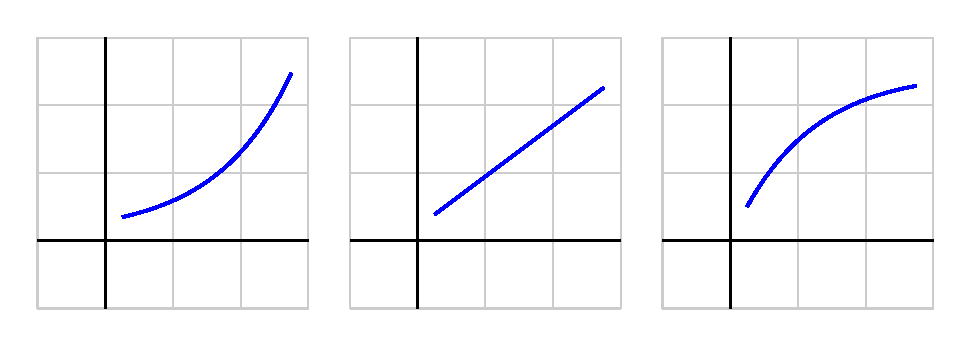
\includegraphics{figures/1_6_3optsi.eps}}
\caption{Three functions that are all increasing, but doing so at an increasing rate, at a constant rate, and at a decreasing rate, respectively.} \label{F:1.6.3optsi}
\end{center}
\end{figure}

For the leftmost curve in Figure~\ref{F:1.6.3optsi}, picture a sequence of tangent lines to the curve.  As we move from left to right, the slopes of those tangent lines will increase.  Therefore, the rate of change of the pictured function is increasing, and this explains why we say this function is \emph{increasing at an increasing rate}.  For the rightmost graph in Figure~\ref{F:1.6.3optsi}, observe that as $x$ increases, the function increases but the slope of the tangent line decreases, hence this function is \emph{increasing at a decreasing rate}.

Of course, similar options hold for how a function can decrease.  Here we must be extra careful with our language, since decreasing functions involve negative slopes, and negative numbers present an interesting situation in the tension between common language and mathematical language.  For example, it can be tempting to say that ``$-100$ is bigger than $-2$.''  But we must remember that when we say one number is greater than another, this describes how the numbers lie on a number line:  $x < y$ provided that $x$ lies to the left of $y$.  So of course, $-100$ is less than $-2$.  Informally, it might be helpful to say that ``$-100$ is more negative than $-2$.''  This leads us to note particularly that when a function's values are negative, and those values subsequently get more negative, the function must be decreasing.

Now consider the three graphs shown in Figure~\ref{F:1.6.3optsd}.  Clearly the middle graph demonstrates the behavior of a function decreasing at a constant rate.  If we think about a sequence of tangent lines to the first curve that progress from left to right, we see that the slopes of these lines get less and less negative as we move from left to right.  That means that the values of the first derivative, while all negative, are increasing, and thus we say that the leftmost curve is \emph{decreasing at an increasing rate}.

\begin{figure}[ht]
\begin{center}
\scalebox{0.9}{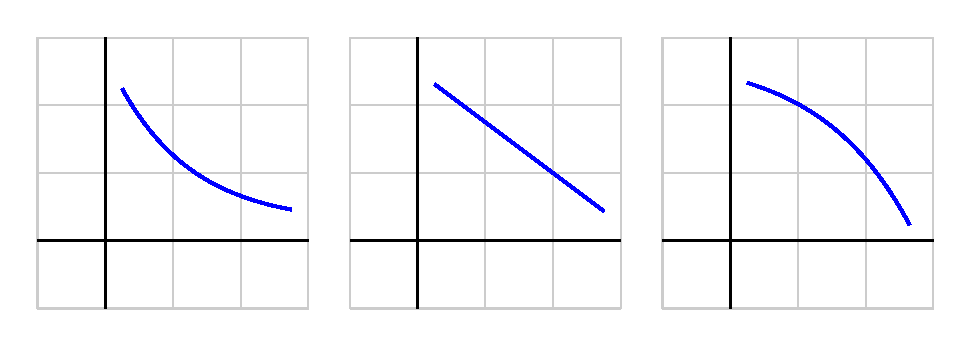
\includegraphics{figures/1_6_3optsd.eps}}
\caption{From left to right, three functions that are all decreasing, but doing so in different ways.} \label{F:1.6.3optsd}
\end{center}
\end{figure}

This leaves only the rightmost curve in Figure~\ref{F:1.6.3optsd} to consider.  For that function, the slope of the tangent line is negative throughout the pictured interval, but as we move from left to right, the slopes get more and more negative.  Hence the slope of the curve is decreasing, and we say that the function is \emph{decreasing at a decreasing rate}.

This leads us to introduce the notion of \emph{concavity} \index{concavity} which provides simpler language to describe some of these behaviors.  Informally, when a curve opens up on a given interval, like the upright parabola $y = x^2$ or the exponential growth function $y = e^x$, we say that the curve is \emph{concave up} on that interval.  Likewise, when a curve opens down, such as the parabola $y = -x^2$ or the opposite of the exponential function $y = -e^{x}$, we say that the function is \emph{concave down}.  This behavior is linked to both the first and second derivatives of the function.  

In Figure~\ref{F:1.6.concavity}, we see two functions along with a sequence of tangent lines to each.  On the lefthand plot where the function is concave up, observe that the tangent lines to the curve always lie below the curve itself and that, as we move from left to right, the slope of the tangent line is increasing.  Said differently, the function $f$ is concave up on the interval shown because its derivative, $f'$, is increasing on that interval.  Similarly, on the righthand plot in Figure~\ref{F:1.6.concavity}, where the function shown is concave down, there we see that the tangent lines alway lie above the curve and that the value of the slope of the tangent line is decreasing as we move from left to right.  Hence, what makes $f$ concave down on the interval is the fact that its derivative, $f'$, is decreasing.

\begin{figure}[ht]
\begin{center}
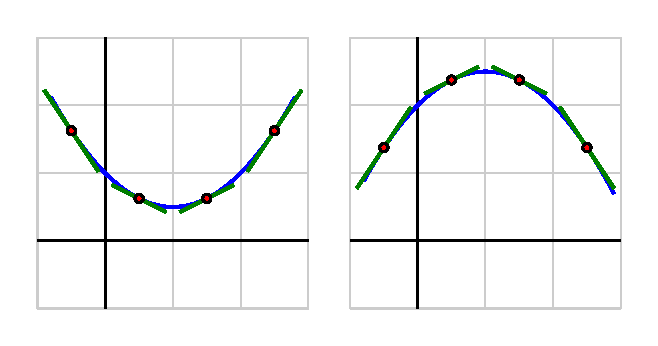
\includegraphics{figures/1_6_concavity.eps}
\caption{At left, a function that is concave up; at right, one that is concave down.} \label{F:1.6.concavity}
\end{center}
\end{figure}

We state these most recent observations formally as the definitions of the terms \emph{concave up} and \emph{concave down}.

\begin{definition}
Let $f$ be a differentiable function on an interval $(a,b)$.  Then $f$ is \emph{concave up} \index{concave up} on $(a,b)$ if and only if $f'$ is increasing on $(a,b)$;  $f$ is \emph{concave down} \index{concave down} on $(a,b)$ if and only if $f'$ is decreasing on $(a,b)$.
\end{definition}

The following activities lead us to further explore how the first and second derivatives of a function determine the behavior and shape of its graph.  We begin by revisiting Preview Activity~\ref{PA:1.6}.

\begin{activity} \label{A:1.6.1}
The position of a car driving along a straight road at time $t$ in minutes is given by the function $y = s(t)$ that is pictured in Figure~\ref{F:1.6.A1}.  The car's position function has units measured in thousands of feet.  Remember that you worked with this function and sketched graphs of $y = v(t) = s'(t)$ and $y = v'(t)$ in Preview Activity~\ref{PA:1.6}.
\begin{figure}[h]
\begin{center}
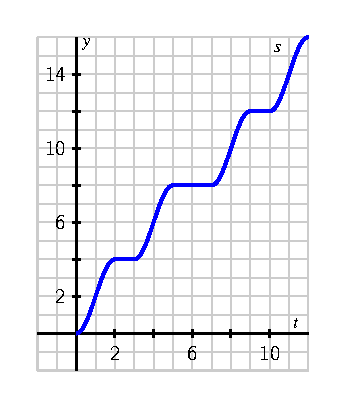
\includegraphics{figures/1_6_PA1.eps}
\caption{The graph of $y = s(t)$, the position of the car (measured in thousands of feet from its starting location) at time $t$ in minutes.} \label{F:1.6.A1}
\end{center}
\end{figure}
\begin{enumerate}
	\item On what intervals is the position function $y = s(t)$ increasing? decreasing?  Why?
	\item On which intervals is the velocity function $y = v(t) = s'(t)$ increasing? decreasing? neither?  Why?
	\item \emph{Acceleration} \index{acceleration} is defined to be the instantaneous rate of change of velocity, as the acceleration of an object measures the rate at which the velocity of the object is changing.  Say that the car's acceleration function is named $a(t)$.  How is $a(t)$ computed from $v(t)$?  How is $a(t)$ computed from $s(t)$?  Explain.
	\item What can you say about $s''$ whenever $s'$ is increasing?  Why?
	\item Using only the words \emph{increasing}, \emph{decreasing}, \emph{constant}, \emph{concave up}, \emph{concave down}, and \emph{linear}, complete the following sentences.  For the position function $s$ with velocity $v$ and acceleration $a$,
	\begin{itemize}
		\item on an interval where $v$ is positive, $s$ is \underline{}.
		\item on an interval where $v$ is negative, $s$ is \underline{}. 
		\item on an interval where $v$ is zero, $s$ is \underline{}.

		\item on an interval where $a$ is positive, $v$ is \underline{}.
		\item on an interval where $a$ is negative, $v$ is \underline{}. 
		\item on an interval where $a$ is zero, $v$ is \underline{}.

		\item on an interval where $a$ is positive, $s$ is \underline{}.
		\item on an interval where $a$ is negative, $s$ is \underline{}. 
		\item on an interval where $a$ is zero, $s$ is \underline{}.
	\end{itemize}
\end{enumerate}

\end{activity}
\begin{hint}[smallhint]
\begin{enumerate}
	\item Remember that a function is increasing on an interval if and only if its first derivative is positive on the interval.
	\item See (a).
	\item Remember that the first derivative of a function measures its instantaneous rate of change.
	\item Think about how $s''(t) = [s'(t)]'$.
	\item Be very careful with your letters:  $s$, $v$, and $a$. 
\end{enumerate}
\end{hint}
\begin{hint}[bighint]
\begin{enumerate}
	\item Remember that a function is increasing on an interval if and only if its first derivative is positive on the interval and that $v(t) = s'(t)$.
	\item See (a), and note that $v'(t) = s''(t)$.
	\item Remember that the first derivative of a function measures its instantaneous rate of change, so $s''(t)$ measures the instantaneous rate of change of $v(t) = s'(t)$.
	\item Note that $s''(t) = [s'(t)]'$, so $s''(t)$ is the slope of the tangent line to $y = s'(t)$.
	\item Be very careful with your letters:  $s$, $v$, and $a$.  For instance, note that when acceleration is positive, velocity must be increasing.
\end{enumerate}
\end{hint}
\begin{solution}
\begin{enumerate}
	\item The position function $y = s(t)$ increasing on the intervals $0<t<2$, $3<t<5$, $7<t<9$, and $10<t<12$, because at every point in such intervals, $s'(t)$ is positive.  For the provided function, $s(t)$ is never decreasing because its derivative is never negative.
	\item The velocity function $y = v(t)$ appears to be increasing on the intervals $0<t<1$, $3<t<4$, $7<t<8$, and $10<t<11$ because the curve $y = s(t)$ is concave up which corresponds to an increasing first derivative $y =s'(t)$.  Similarly, $y = v(t)$ appears to be decreasing on the intervals $1<t<2$, $4<t<5$, $8<t<9$, and $11<t<12$ because the curve $y = s(t)$ is concave down which corresponds to a decreasing first derivative $y =s'(t)$.  On the intervals $2<t<3$, $5<t<7$, and $9<t<10$, the curve $y = s(t)$ is constant, and thus linear, so neither concave up nor concave down.  
	\item Since $a(t)$ is the instantaneous rate of change of $v(t)$, $a(t) = v'(t)$.  And because $v(t) = s'(t)$, it follows that $a(t) = v'(t) = [s'(t)]' = s''(t)$, so acceleration is the second derivative of position. 
	\item Because $s''(t)$ is the first derivative of $s'(t)$, when $s'(t)$ is increasing, $s''(t)$ must be positive.
	\item For the position function $s(t)$ with velocity $v(t)$ and acceleration $a(t)$,
	\begin{itemize}
		\item on an interval where $v(t)$ is positive, $s(t)$ is \underline{increasing}.
		\item on an interval where $v(t)$ is negative, $s(t)$ is \underline{decreasing}. 
		\item on an interval where $v(t)$ is zero, $s(t)$ is \underline{constant}.

		\item on an interval where $a(t)$ is positive, $v(t)$ is \underline{increasing}.
		\item on an interval where $a(t)$ is negative, $v(t)$ is \underline{decreasing}. 
		\item on an interval where $a(t)$ is zero, $v(t)$ is \underline{constant}.

		\item on an interval where $a(t)$ is positive, $s(t)$ is \underline{concave up}.
		\item on an interval where $a(t)$ is negative, $s(t)$ is \underline{concave down}. 
		\item on an interval where $a(t)$ is zero, $s(t)$ is \underline{linear}.
	\end{itemize}
\end{enumerate}
\end{solution}

The context of position, velocity, and acceleration is an excellent one in which to understand how a function, its first derivative, and its second derivative are related to one another.  In Activity~\ref{A:1.6.1}, we can replace $s$, $v$, and $a$ with an arbitrary function $f$ and its derivatives $f'$ and $f''$, and essentially all the same observations hold.  In particular, note that $f'$ is increasing if and only if both $f$ is concave up, and similarly $f'$ is increasing if and only if $f''$ is positive.  Likewise, $f'$ is decreasing if and only if both $f$ is concave down, and $f'$ is decreasing if and only if $f''$ is negative.

\begin{activity} \label{A:1.6.3}
A potato is placed in an oven, and the potato's temperature $F$ (in degrees Fahrenheit) at various points in time is taken and recorded in the following table. Time $t$ is measured in minutes.  In Activity~\ref{A:1.5.1}, we computed approximations to $F'(30)$ and $F'(60)$ using central differences.  Those values and more are provided in the second table below, along with several others computed in the same way.

\begin{center}
\begin{tabular}{cc}
\begin{tabular}{| l || l |}
\hline
$t$ & $F(t)$ \\ \hline \hline
0 & 70\\ \hline
15 & 180.5 \\ \hline
30 & 251 \\ \hline
45 & 296 \\ \hline
60 & 324.5 \\ \hline
75 & 342.8 \\ \hline
90 & 354.5  \\ \hline
\end{tabular}
&
\begin{tabular}{| l || l |}
\hline
$t$ & $F'(t)$ \\ \hline \hline
0 & NA\\ \hline
15 & 6.03 \\ \hline
30 & 3.85 \\ \hline
45 & 2.45 \\ \hline
60 & 1.56 \\ \hline
75 & 1.00 \\ \hline
90 & NA  \\ \hline
\end{tabular}
\end{tabular}
\end{center}
\begin{enumerate}
	\item What are the units on the values of $F'(t)$? 
	\item Use a central difference to estimate the value of $F''(30)$.
	\item What is the meaning of the value of $F''(30)$ that you have computed in (b) in terms of the potato's temperature?  Write several careful sentences that discuss, with appropriate units, the values of $F(30)$, $F'(30)$, and $F''(30)$, and explain the overall behavior of the potato's temperature at this point in time.
	\item Overall, is the potato's temperature increasing at an increasing rate, increasing at a constant rate, or increasing at a decreasing rate?  Why?
\end{enumerate}

\end{activity}
\begin{hint}[smallhint]
\begin{enumerate}
	\item Remember that the derivative's units are ``units of output per unit of input.'' 
	\item To estimate $g'(a)$, we can use 
	$$g'(a) \approx \frac{g(a+h)-g(a-h)}{2h}$$
	for an appropriate choice of $h$.
	\item For each of the values $F'(30)$ and $F''(30)$, think about what they tell you about expected upcoming behavior in $F(t)$ and $F'(t)$, respectively.
	\item Think concavity.
\end{enumerate}
\end{hint}
\begin{hint}[bighint]
\begin{enumerate}
	\item Remember that the derivative's units are ``units of output per unit of input.'' 
	\item To estimate $g'(a)$, we can use 
	$$g'(a) \approx \frac{g(a+h)-g(a-h)}{2h}$$
	for an appropriate choice of $h$.  So, observe that
	$$F''(a) \approx \frac{F'(a+h)-F'(a-h)}{2h}$$
	\item For each of the values $F'(30)$ and $F''(30)$, think about what they tell you about expected upcoming behavior in $F(t)$ and $F'(t)$, respectively.  What do you expect to be the values of $F(31)$ and $F'(31)$?  Why?
	\item Examine the given data and think about how the graph of $y = F(t)$ will appear.
\end{enumerate}
\end{hint}
\begin{solution}
\begin{enumerate}
	\item $F'(t)$ has units measured in degrees Fahrenheit per minute. 
	\item Using a central difference, 
	$$F''(30) \approx \frac{F'(45)-F'(15)}{30} = \frac{2.45-6.03}{30} \approx -0.119.$$
	\item The value $F''(30) \approx -0.119$, which is measured in degrees per minute per minute tells us, along with the other data, that at the moment $t = 30$, the temperature of the potato is 251 degrees, that its temperature is rising at a rate of 3.85 degrees per minute, and that the rate at which the temperature is rising is \emph{falling} at a rate of -0.119 degrees per minute per minute.  That is, while the temperature is rising, it is rising at a slower and slower rate.  At $t = 31$, we'd expect that the rate of increase of the potato's temperature would have dropped to about 3.73 degrees per minute.
	\item The potato's temperature increasing at a decreasing rate because the values of the first derivative of $F$ are falling.  Equivalently, this is because the value of $F''(t)$ is negative throughout the given time interval.
\end{enumerate}
\end{solution}


\begin{activity} \label{A:1.6.2}
This activity builds on our experience and understanding of how to sketch the graph of $f'$ given the graph of $f$.  

\begin{figure}[h]
\begin{center}
\includegraphics{figures/1_6_Act2.eps}
\caption{Two given functions $f$, with axes provided for plotting $f'$ and $f''$ below.} \label{F:1.6.A2}
\end{center}
\end{figure}

 In Figure~\ref{F:1.6.A2}, given the respective graphs of two different functions $f$, sketch the corresponding graph of $f'$ on the first axes below, and then sketch $f''$ on the second set of axes.  In addition, for each, write several careful sentences in the spirit of those in Activity~\ref{A:1.6.1} that connect the behaviors of $f$, $f'$, and $f''$.  For instance, write something such as
\begin{quote}
$f'$ is \underline{} on the interval \underline{}, which is connected to the fact that $f$ is \underline{} on the same interval \underline{}, and $f''$ is \underline{} on the interval as well
\end{quote}
but of course with the blanks filled in.  Throughout, view the scale of the grid for the graph of $f$ as being $1 \times 1$, and assume the horizontal scale of the grid for the graph of $f'$ is identical to that for $f$.  If you need to adjust the vertical scale on the axes for the graph of $f'$ or $f''$, you should label that accordingly.

\end{activity}
\begin{hint}[smallhint]
Remember that to plot $y = f'(x)$, it is helpful to first identify where $f'(x) = 0.$
\end{hint}
\begin{hint}[bighint]
Remember that to plot $y = f'(x)$, it is helpful to first identify where $f'(x) = 0$, and then ask where $y = f'(x)$ is positive and negative.  In a similar way, once $y = f'(x)$ has been plotted, to construct the graph of $y=f''(x)$, it is useful to note where the slope of the tangent line to $y = f'(x)$ is zero, as well as where such slopes are positive and negative.  Heights on the graph of $y = f''(x)$ will correspond to slopes on $y = f'(x)$.
\end{hint}
\begin{solution}
The graphs of $f'$ and $f''$ are plotted in Figure~***.
\end{solution}

\begin{authornote}
This is an author note.
\end{authornote}

\begin{summary}
\item A differentiable function $f$ is increasing at a point or on an interval whenever its first derivative is positive, and decreasing whenever its first derivative is negative.
\item By taking the derivative of the derivative of a function $f$, we arrive at the second derivative, $f''$.  The second derivative measures the instantaneous rate of change of the first derivative, and thus the sign of the second derivative tells us whether or not the slope of the tangent line to $f$ is increasing or decreasing.
\item A differentiable function is concave up whenever its first derivative is increasing (or equivalently whenever its second derivative is positive), and concave down whenever its first derivative is decreasing (or equivalently whenever its second derivative is negative).  Examples of functions that are everywhere concave up are $y = x^2$ and $y = e^x$; examples of functions that are everywhere concave down are $y = -x^2$ and $y = -e^x$.
\item The units on the second derivative are ``units of output per unit of input per unit of input.''  They tell us how the value of the derivative function is changing in response to changes in the input.  In other words, the second derivative tells us the rate of change of the rate of change of the original function.
\end{summary}



\begin{exercises}
\begin{enumerate}
\begin{enumerate} 
\item Suppose that $y = f(x)$ is a differentiable function for which the following information is known:  $f(2) = -3$, $f'(2) = 1.5$, $f''(2) = -0.25$.
\begin{enumerate}
	\item Is $f$ increasing or decreasing at $x = 2$?  Is $f$ concave up or concave down at $x = 2$?
	\item Do you expect $f(2.1)$ to be greater than $-3$, equal to $-3$, or less than $-3$?  Why?
	\item Do you expect $f'(2.1)$ to be greater than $1.5$, equal to $1.5$, or less than $1.5$?  Why?
	\item Sketch a graph of $y = f(x)$ near $(2,f(2))$ and include a graph of the tangent line.  
\end{enumerate}
\begin{solution}
\end{solution}
\item For a certain function $y = g(x)$, its derivative is given by the function pictured in Figure~\ref{F:1.6.Ez2}.
\begin{figure}[ht]
\begin{center}
\includegraphics{figures/1_6_Ez2.eps}
\caption{The graph of $y = g'(x)$.} \label{F:1.6.Ez2}
\end{center}
\end{figure}
\begin{enumerate}
	\item What is the approximate slope of the tangent line to $y = g(x)$ at the point $(2,g(2))$?
	\item How many real number solutions can there be to the equation $g(x) = 0$?  Justify your conclusion fully and carefully by explaining what you know about how the graph of $g$ must behave based on the given graph of $g'$.
	\item On the interval $-3 < x < 3$, how many times does the concavity of $g$ change?  Why?
	\item Use the provided graph to estimate the value of $g''(2)$.
\end{enumerate}
\item A bungee jumper's height $h$ (in feet ) at time $t$ (in seconds) is given in part by the data in the following table:

\begin{tabular}{ l | l | l | l |  l | l | l | l | l | l | l | l }
$t$ & 0.0 & 0.5 & 1.0 & 1.5 & 2.0 & 2.5 & 3.0 & 3.5 & 4.0 & 4.5 & 5.0    \\ \hline 

$h(t)$ & 200 & 184.2 &  159.9 &  131.9 &  104.7 & 81.8 &  65.5 &  56.8 &  55.5 & 60.4 & 69.8 
 
\end{tabular}

\begin{tabular}{ l | l | l | l |  l | l | l | l | l | l | l  }
$t$ & 5.5 & 6.0 & 6.5 & 7.0 & 7.5 & 8.0 & 8.5 & 9.0 & 9.5 & 10.0 \\ \hline 
$h(t)$ & 81.6 & 93.7 &  104.4 &  112.6 &  117.7 & 119.4 & 118.2 & 114.8 &  110.0 &  104.7
 
\end{tabular}

\begin{enumerate}
	\item Use the given data to estimate $h'(4.5)$, $h'(5)$, and $h'(5.5)$.  At which of these times is the bungee jumper rising most rapidly?
	\item Use the given data and your work in (a) to estimate $h''(5)$.
	\item What physical property of the bungee jumper does the value of $h''(5)$ measure?  What are its units?
	\item Based on the data, on what approximate time intervals is the function $y = h(t)$ concave down?  What is happening to the velocity of the bungee jumper on these time intervals?
\end{enumerate}

\item For each prompt that follows, sketch a possible graph of a function on the interval $-3 < x < 3$ that satisfies the stated properties.
\begin{enumerate}
	\item $y = f(x)$ such that $f$ is increasing on $-3 < x < 3$, $f$ is concave up on $-3 < x < 0$, and $f$ is concave down on $0 < x < 3$.
	\item $y = g(x)$ such that $g$ is increasing on $-3 < x < 3$, $g$ is concave down on $-3 < x < 0$, and $g$ is concave up on $0 < x < 3$.
	\item $y = h(x)$ such that $h$ is decreasing on $-3 < x < 3$, $h$ is concave up on $-3 < x < -1$, neither concave up nor concave down on $-1 < x < 1$, and $h$ is concave down on $1 < x < 3$.
	\item $y = p(x)$ such that $p$ is decreasing and concave down on $-3 < x < 0$ and $p$ is increasing and concave down on $0 < x < 3$.
\end{enumerate}

\end{enumerate}
\end{enumerate}
\end{exercises} 

\clearpage
\section{Limits, Continuity, and Differentiability} \label{S:1.7.LimContDiff}

\vspace{-14 pt}

In this section, we strive to understand the ideas generated by the following important questions:
\begin{objectives}
\begin{itemize}
\item What does it mean graphically to say that $f$ has limit $L$ as $x \to a$?  How is this connected to having a left-hand limit at $x = a$ and having a right-hand limit at $x = a$?
\item What does it mean to say that a function $f$ is continuous at $x = a$?  What role do limits play in determining whether or not a function is continuous at a point?
\item What does it mean graphically to say that a function $f$ is differentiable at $x = a$?  How is this connected to the function being locally linear? 
\item How are the characteristics of a function having a limit, being continuous, and being differentiable at a given point related to one another?
\end{itemize}\end{objectives} 

\subsection*{Introduction}
In Section~\ref{S:1.2.Limits}, we learned about how the concept of limits can be used to study the trend of a function near a fixed input value.  As we study such trends, we are fundamentally interested in knowing how well-behaved the function is at the given point, say $x = a$.  In this present section, we aim to expand our perspective and develop language and understanding to quantify how the function acts and how its value changes near a particular point.  Beyond thinking about whether or not the function has a limit $L$ at $x = a$, we will also consider the value of the function $f(a)$ and how this value is related to $\lim_{x \to a} f(x)$, as well as whether or not the function has a derivative $f'(a)$ at the point of interest.  Throughout,  we will build on and formalize ideas that we have encountered in several settings.

We begin to consider these issues through the following preview activity that asks you to consider the graph of a function with a variety of interesting behaviors.

\begin{previewactivity} \label{PA:1.7}
A function $f$ defined on $-4 < x < 4$ is given by the graph in Figure~\ref{F:1.7.PA1}.  Use the graph to answer each of the following questions.  Note: to the right of $x = 2$, the graph of $f$ is exhibiting infinite oscillatory behavior similar to the function $\sin(\frac{\pi}{x})$ that we encountered in the key example early in Section~\ref{S:1.2.Limits}.
\begin{figure}[h]
\begin{center}
\includegraphics{figures/1_7_PA1.eps}
\caption{The graph of $y = f(x)$.} \label{F:1.7.PA1}
\end{center}
\end{figure}
\begin{enumerate}
	\item For each of the values $a = -3, -2, -1, 0, 1, 2, 3$, determine whether or not $\ds \lim_{x \to a} f(x)$ exists.  If the function has a limit $L$ at a given point, state the value of the limit using the notation $\ds \lim_{x \to a} f(x) = L$.  If the function does not have a limit at a given point, write a sentence to explain why.
	\item For each of the values of $a$ from part (a) where $f$ has a limit, determine the value of $f(a)$ at each such point.  In addition, for each such $a$ value, does $f(a)$ have the same value as $\ds \lim_{x \to a} f(x)$?
	\item For each of the values $a = -3, -2, -1, 0, 1, 2, 3$, determine whether or not $f'(a)$ exists.  In particular, based on the given graph, ask yourself if it is reasonable to say that $f$ has a tangent line at $(a,f(a))$ for each of the given $a$-values.  If so, visually estimate the slope of the tangent line to find the value of $f'(a)$.
\end{enumerate}
\end{previewactivity} 




\subsection*{Having a limit at a point}

In Section~\ref{S:1.2.Limits}, we first encountered limits and learned that we say that $f$ has limit $L$ as $x$ approaches $a$ and write $\ds \lim_{x \to a} f(x) = L$ provided that we can make the value of $f(x)$ as close to $L$ as we like by taking $x$ sufficiently close (but not equal to) $a$.  Here, we expand further on this definition and focus in more depth on what it means for a function not to have a limit at a given value.  

Essentially there are two behaviors that a function can exhibit at a point where it fails to have a limit.  In Figure~\ref{F:1.7.NoLimit}, at left we see a function $f$ whose graph shows a jump at $a = 1$.  In particular, if we let $x$ approach 1 from the left side, the value of $f$ approaches 2, while if we let $x$ go to $1$ from the right, the value of $f$ tends to 3.  Because the value of $f$ does not approach a single number as $x$ gets arbitrarily close to 1 from both sides, we know that $f$ does not have a limit at $a = 1$.  

Since $f$ does approach a single value on each side of $a = 1$, we can introduce the notion of \emph{left} and \emph{right}  (or \emph{one-sided}) limits. \index{left limit} \index{right limit} \index{limit!one-sided}  We say that \emph{$f$ has limit $L_1$ as $x$ approaches $a $ from the left} and write
$$\lim_{x \to a^-} f(x) = L_1$$
 provided that we can make the value of $f(x)$ as close to $L_1$ as we like by taking $x$ sufficiently close to $a$ while always having $x < a$.  In this case, we call $L_1$ the left-hand limit of $f$ as $x$ approaches $a$.  Similarly, we say \emph{$L_2$ is the right-hand limit of $f$ as $x$ approaches $a$} and write
$$\lim_{x \to a^+} f(x) = L_2$$
provided that we can make the value of $f(x)$ as close to $L_2$ as we like by taking $x$ sufficiently close to $a$ while always having $x > a$.  In the graph of the function $f$ in Figure~\ref{F:1.7.NoLimit}, we see that 
$$\lim_{x \to 1^-} f(x) = 2 \ \ \mbox{and} \ \lim_{x \to 1^+} f(x) = 3$$
and precisely because the left and right limits are not equal, the overall limit of $f$ as $x \to 1$ fails to exist.

\begin{figure}[h]
\begin{center}
\scalebox{0.9}{\includegraphics{figures/1_7_NoLimit.eps}}
\caption{Functions $f$ and $g$ that each fail to have a limit at $a = 1$.} \label{F:1.7.NoLimit}
\end{center}
\end{figure}

For the function $g$ pictured at right in Figure~\ref{F:1.7.NoLimit}, the function fails to have a limit at $a = 1$ for a different reason.  While the function does not have a jump in its graph at $a = 1$, it is still not the case that $g$ approaches a single value as $x$ approaches 1.  In particular, due to the infinitely oscillating behavior of $g$ to the right of $a = 1$, we say that the right-hand limit of $g$ as $x \to 1^+$ does not exist, and thus 
$\ds \lim_{x \to 1} g(x) \ \mbox{does not exist}.$

To summarize, anytime either a left- or right-hand limit fails to exist or the left- and right-hand limits are not equal to each other, the overall limit will not exist.  Said differently, 

\vspace{5pt}
 

A function $f$ has limit $L$ as $x \to a$ if and only if
$$\lim_{x \to a^-} f(x) = L = \lim_{x \to a^+} f(x).$$
That is, a function has a limit at $x = a$ if and only if both the left- and right-hand limits at $x = a$ exist and share the same value.
 
\vspace{1pt}

In Preview Activity~\ref{PA:1.7}, the function $f$ given in Figure~\ref{F:1.7.PA1} only fails to have a limit at two values:  at $a = -2$ (where the left- and right-hand limits are 2 and $-1$, respectively) and at $x = 2$, where $\lim_{x \to 2^+} f(x)$ does not exist).  Note well that even at values like $a = -1$ and $a = 0$ where there are holes in the graph, the limit still exists. 

\begin{activity} \label{A:1.7.1}
Consider a function that is piecewise-defined according to the formula
$$f(x) = \begin{cases}

  3(x+2)+2 & \text{for $-3 < x < -2$} \\
  \frac{2}{3}(x+2)+1 & \text{for $-2 \le x < -1$} \\
  \frac{2}{3}(x+2)+1 & \text{for $-1 < x < 1$} \\
  2 & \text{for $x = 1$} \\
  4-x & \text{for $x > 1$}

\end{cases}$$
Use the given formula to answer the following questions.
\begin{figure}[h]
\begin{center}
\includegraphics{figures/1_7_Act1.eps}
\caption{Axes for plotting the function $y = f(x)$ in Activity~\ref{A:1.7.1}.} \label{F:1.7.Act1}
\end{center}
\end{figure}
\begin{enumerate}
	\item For each of the values $a = -2, -1, 0, 1, 2$, compute $f(a)$.
	\item For each of the values $a = -2, -1, 0, 1, 2$, determine $\ds \lim_{x \to a^-} f(x)$ and $\ds \lim_{x \to a^+} f(x)$.  
	\item For each of the values $a = -2, -1, 0, 1, 2$, determine $\ds \lim_{x \to a} f(x)$.  If the limit fails to exist, explain why by discussing the left- and right-hand limits at the relevant $a$-value.
	\item For which values of $a$ is the following statement true?
	$$\lim_{x \to a} f(x) \ne f(a)$$
	\item On the axes provided in Figure~\ref{F:1.7.Act1}, sketch an accurate, labeled graph of $y = f(x)$.  Be sure to carefully use open circles ($\circ$) and filled circles ($\bullet$) to represent key points on the graph, as dictated by the piecewise formula.
\end{enumerate}

\end{activity}
\begin{hint}[smallhint]
\begin{enumerate}
	\item Find the interval in which $a$ lies and evaluate the function there.
	\item Remember that for $\ds \lim_{x \to a^-} f(x)$, we only consider values of $x$ such that $x < a$.  Find the right formula to use in the piecewise definition for $f$ to fit the values you are considering.
	\item Use your work in (c) and compare left- and right-hand limits.
	\item Use your work in (a) and (c).
	\item Note that $f$ is piecewise linear.  
\end{enumerate}
\end{hint}
\begin{hint}[bighint]
\begin{enumerate}
	\item Find the interval in which $a$ lies and evaluate the function there.  For example, $f(-2) = \frac{2}{3}(-2+2) + 1$, based on the formula for $f$.
	\item Remember that for $\ds \lim_{x \to a^-} f(x)$, we only consider values of $x$ such that $x < a$.  Find the right formula to use in the piecewise definition for $f$ to fit the values you are considering.  For example, as $x \to -2^-$, we use the formula $3(x+2)+2$ and see that $3(x+2)+2 \to 3(-2+2)+2 = 2$ as $x \to -2^+$.
	\item Use your work in (c) and compare left- and right-hand limits.  Remember that the overall limit exists if and only if both left and right limits exists and are equal in value.
	\item Use your work in (a) and (c).
	\item Note that $f$ is piecewise linear.  For instance, $y = 3(x+2) + 2$ is a line through $(-2,2)$ with slope 3 and is valid on the interval $-3 < x < -2$.
\end{enumerate}\end{hint}
\begin{solution}
\begin{enumerate}
	\item $f(-2) = \frac{2}{3}(-2+2) + 1 = 1$; $f(-1)$ is not defined; $f(0) = \frac{2}{3}(0+2)+1 = \frac{7}{3}$; $f(1) = 2$ (by the rule); $f(2) = 4-2 = 2$.
	\item $$\lim_{x \to -2^-} f(x) = 2 \ \mbox{and} \lim_{x \to -2^+} f(x) = 1$$
	        $$\lim_{x \to -1^-} f(x) = \frac{5}{3} \ \mbox{and} \lim_{x \to -1^+} f(x) = \frac{5}{3}$$
	        $$\lim_{x \to 0^-} f(x) = \frac{7}{3} \ \mbox{and} \lim_{x \to 0^+} f(x) = \frac{7}{3}$$
	        $$\lim_{x \to 1^-} f(x) = 3 \ \mbox{and} \lim_{x \to 1^+} f(x) = 3$$
	        $$\lim_{x \to 2^-} f(x) = 2 \ \mbox{and} \lim_{x \to 2^+} f(x) = 2$$
	\item $\ds \lim_{x \to -2} f(x)$ does not exists because the left-hand limit is $2$ while the right-hand limit is $1$.  All of the other requested limits exist, as left- and right-hand limits exist and are equal in each case.  The respective values of the limits as $x \to a$ for $a = -1, 0, 1, 2$ are $\frac{5}{3}, \frac{7}{3}, 3, 2$.
	\item For $a = -2$, $a = -1$, and $a = 1$, $\ds \lim_{x \to a} f(x) \ne f(a)$.  At $a = -2$, the limit fails to exist, but $f(-2) = 1$.  At $a = -1$, the limit is $\frac{5}{3}$, but $f(-1)$ is not defined.  At $a = 1$, the limit is 3, but $f(1) = 2$.
	\item \includegraphics{figures/1_7_Act1Soln.eps}
\end{enumerate}	        
\end{solution}

\subsection*{Being continuous at a point} \index{continuous}

Intuitively, a function is continuous if we can draw it without ever lifting our pencil from the page.  Alternatively, we might say that the graph of a continuous function has no jumps or holes in it.  We first consider three specific situations in Figure~\ref{F:1.7.Cont} where all three functions have a limit at $a = 1$, and then work to make the idea of continuity more precise.

\begin{figure}[h]
\begin{center}
\scalebox{0.9}{\includegraphics{figures/1_7_Cont.eps}}
\caption{Functions $f$, $g$, and $h$ that demonstrate subtly different behaviors at $a = 1$.} \label{F:1.7.Cont}
\end{center}
\end{figure}

Note that  $f(1)$ is not defined, which leads to the resulting hole in the graph of $f$ at $a = 1$.  We will naturally say that $f$ is \emph{not continuous at $a = 1$}.  For the next function $g$ in in Figure~\ref{F:1.7.Cont}, we observe that while $\lim_{x \to 1} g(x) = 3$, the value of $g(1) = 2$, and thus the limit does not equal the function value.  Here, too, we will say that $g$ is \emph{not continuous}, even though the function is defined at $a = 1$.  Finally, the function $h$ appears to be the most well-behaved of all three, since at $a = 1$ its limit and its function value agree.  That is,
$$\lim_{x \to 1} h(x) = 3 = h(1).$$
With no hole or jump in the graph of $h$ at $a = 1$, we desire to say that $h$ is \emph{continuous} there.

More formally, we make the following definition.
\begin{definition} 
A function $f$ is \emph{continuous at $x = a$} \index{continuous at $x = a$} provided that
\begin{enumerate}
	\item $f$ has a limit as $x \to a$,
	\item $f$ is defined at $x = a$, and
	\item $\ds \lim_{x \to a} f(x) = f(a).$
\end{enumerate}
\end{definition}
Conditions (a) and (b) are technically contained implicitly in (c), but we state them explicitly to emphasize their individual importance.  In words, (c) essentially says that a function is continuous at $x = a$ provided that its limit as $x \to a$ exists and equals its function value at $x = a$.  If a function is continuous at every point in an interval $[a,b]$, we say the function is ``continuous on $[a,b]$.''  If a function is continuous at every point in its domain, we simply say the function is ``continuous.'' Thus, continuous functions are particularly nice:  to evaluate the limit of a continuous function at a point, all we need to do is evaluate the function.

For example, consider $p(x) = x^2 - 2x + 3$.  It can be proved that every polynomial is a continuous function at every real number, and thus if we would like to know $\lim_{x \to 2} p(x)$, we simply compute
$$\lim_{x \to 2} (x^2 - 2x + 3) = 2^2 - 2 \cdot 2 + 3 = 3.$$
This route of substituting an input value to evaluate a limit works anytime we know function being considered is continuous.  Besides polynomial functions, all exponential functions and the sine and cosine functions are continuous at every point, as are many other familiar functions and combinations thereof.  

\begin{activity} \label{A:1.7.2}
This activity builds on your work in Preview Activity~\ref{PA:1.7}, using the same function $f$ as given by the graph that is repeated in Figure~\ref{F:1.7.A2}
\begin{figure}[h]
\begin{center}
\includegraphics{figures/1_7_PA1.eps}
\caption{The graph of $y = f(x)$ for Activity~\ref{A:1.7.2}.} \label{F:1.7.A2}
\end{center}
\end{figure}
\begin{enumerate}
	\item At which values of $a$ does $\lim_{x \to a} f(x)$ not exist?
	\item At which values of $a$ is $f(a)$ not defined?
	\item At which values of $a$ does $f$ have a limit, but $\lim_{x \to a} f(x) \ne f(a)$?
	\item State all values of $a$ for which $f$ is not continuous at $x = a$.
	\item Which condition is stronger, and hence implies the other:   $f$  has a limit at $x = a$ or  $f$ is continuous at $x = a$?  Explain, and hence complete the following sentence:  ``If $f$ \underline{} at $x = a$, then $f$ \underline{} at $x = a$,'' where you complete the blanks with \emph{has a limit} and \emph{is continuous}, using each phrase once.
\end{enumerate}
\end{activity}
\begin{hint}[smallhint]
\begin{enumerate}
	\item Consider the left- and right-hand limits at each value.
	\item Carefully examine places on the graph where there's an open circle.
	\item Are there locations on the graph where the function has a limit but there's a hole in the graph?
	\item Remember that at least one of three conditions must fail: if the function lacks a limit, if the function is undefined, or if the limit exists but does not equal the function value, then $f$ is not continuous at the point.
	\item Note that the definition of being continuous requires the limit to exist.
\end{enumerate}
\end{hint}
\begin{hint}[bighint]
\begin{enumerate}
	\item Consider the left- and right-hand limits at each value, and recall that they must both exist and be equal in order for the overall limit to exist.
	\item Carefully examine places on the graph where there's an open circle; at such locations, look vertically to see if the function has an assigned value at that point.
	\item Are there locations on the graph where the function has a limit but there's a hole in the graph?
	\item Remember that at least one of three conditions must fail: if the function lacks a limit, if the function is undefined, or if the limit exists but does not equal the function value, then $f$ is not continuous at the point.
	\item Note that the definition of being continuous requires the limit to exist.
\end{enumerate}
\end{hint}
\begin{solution}
\begin{enumerate}
	\item $\lim_{x \to a} f(x)$ does not exist at $a = -2$ since $\lim_{x \to -2^-} f(x) = 2 \ne -1 = \lim_{x \to -2^+}$ and $\lim_{x \to a} f(x)$ does not exist at $a = +2$ since $\lim_{x \to 2^+} f(x)$ does not exist due to the infinitely oscillatory behavior of $f$.
	\item The only point at which $f$ is not defined is at $a = 3$.
	\item At $x = -1$, note that $\lim_{x \to -1} f(x)$ exists (and appears to have value approximately $-3.25$), but $f(-1) = 1$, and thus $\lim_{x \to -1} f(x) \ne f(-1)$.  At $x = 3$, $\lim_{x \to 3} f(x) = -2.5$, but $f(3)$ is not defined, so the limit exists but does not equal the function value.
	\item Based on our work in (a), (b), and (c), $f$ is not continuous at $a=-2$ and $a = 2$ because $f$ does not have a limit at those points; $f$ is not continuous at $a = 3$ since $f$ is not defined there; and $f$ is not continuous at $a = -1$ because at that point its limit does not equal its function value.
	\item ``If $f$ \underline{is continuous} at $x = a$, then $f$ \underline{has a limit} at $x = a$,'' since one of the defining properties of ``being continuous'' at $x = a$ is that the function has a limit at that input value.  This shows that being continuous is a stronger condition than having a limit.
\end{enumerate}
\end{solution}

\subsection*{Being differentiable at a point} \index{differentiable}

We recall that a function $f$ is said to be differentiable at $x = a$ whenever $f'(a)$ exists.  Moreover, for $f'(a)$ to exist, we know that the function $y = f(x)$ must have a tangent line at the point $(a,f(a))$, since $f'(a)$ is precisely the slope of this line.  In order to even ask if $f$ has a tangent line at $(a,f(a))$, it is necessary that $f$ be continuous at $x = a$: if $f$ fails to have a limit at $x = a$, if $f(a)$ is not defined, or if $f(a)$ does not equal the value of $\lim_{x \to a} f(x)$, then it doesn't even make sense to talk about a tangent line to the curve at this point.

Indeed, it can be proved formally that if a function $f$ is differentiable at $x = a$, then it must be continuous at $x = a$.  So, if $f$ is not continuous at $x = a$, then it is automatically the case that $f$ is not differentiable there.  For example, in Figure~\ref{F:1.7.Cont} from our early discussion of continuity, both $f$ and $g$ fail to be differentiable at $x = 1$ because neither function is continuous at $x = 1$.  But can a function fail to be differentiable at a point where the function is continuous?

In Figure~\ref{F:1.7.NotDiff}, we revisit the situation where a function has a sharp corner at a point, something we encountered several times in Section~\ref{S:1.4.DerivativeFxn}.  For the pictured function $f$, we observe that $f$ is clearly continuous at $a = 1$, since $\lim_{x \to 1} f(x) = 1 = f(1).$

\begin{figure}[ht]
\begin{center}
\includegraphics{figures/1_7_NotDiff.eps}
\caption{A function $f$ that is continuous at $a = 1$ but not differentiable at $a = 1$; at right, we zoom in on the point $(1,1)$ in a magnified version of the box in the left-hand plot.} \label{F:1.7.NotDiff}
\end{center}
\end{figure}

But the function $f$ in Figure~\ref{F:1.7.NotDiff} is not differentiable at $a = 1$ because $f'(1)$ fails to exist.  One way to see this is to observe that $f'(x) = -1$ for every value of $x$ that is less than 1, while $f'(x) = +1$ for every value of $x$ that is greater than 1.  That makes it seem that either $+1$ or $-1$ would be equally good candidates for the value of the derivative at $x = 1$.   Alternately, we could use the limit definition of the derivative to attempt to compute $f'(1)$, and discover that the derivative does not exist.  A similar problem will be investigated in Activity~\ref{A:1.7.3}.  Finally, we can also see visually that the function $f$ in Figure~\ref{F:1.7.NotDiff} does not have a tangent line.  When we zoom in on $(1,1)$ on the graph of $f$, no matter how closely we examine the function, it will always look like a ``V'', and never like a single line, which tells us there is no possibility for a tangent line there.  

To make a more general observation, if a function does have a tangent line at a given point, when we zoom in on the point of tangency, the function and the tangent line should appear essentially indistinguishable\footnote{See, for instance, \href{http://gvsu.edu/s/6J}{\texttt{http://gvsu.edu/s/6J}} for an applet (due to David Austin, GVSU) where zooming in shows the increasing similarity between the tangent line and the curve.  }.  Conversely, if we have a function such that when we zoom in on a point the function looks like a single straight line, then the function should have a tangent line there, and thus be differentiable.  Hence, a function that is differentiable at $x = a$ will, up close, look more and more like its tangent line at $(a,f(a))$, and thus we say that a function is differentiable at $x = a$ is \emph{locally linear}. \index{locally linear}


To summarize the preceding discussion of differentiability and continuity, we make several important observations.
\begin{itemize}
	\item If $f$ is differentiable at $x = a$, then $f$ is continuous at $x = a$.  Equivalently, if$f$ fails to be continuous at $x = a$, then $f$ will not be differentiable at $x = a$.  
	\item A function can be continuous at a point, but not be differentiable there.  In particular, a function $f$ is not differentiable at $x = a$ if the graph has a sharp corner (or \emph{cusp}) \index{cusp} at the point $(a,f(a))$.  
	\item If $f$ is differentiable at $x = a$, then $f$ is locally linear at $x = a$.  That is, when a function is differentiable, it looks linear when viewed up close because it resembles its tangent line there.
\end{itemize}



\begin{activity} \label{A:1.7.3} 
In this activity, we explore two different functions and classify the points at which each is not differentiable.  Let $g$ be the function given by the rule $g(x) = |x|$, and let $f$ be the function that we have previously explored in Preview Activity~\ref{PA:1.7}, whose graph is given again in Figure~\ref{F:1.7.Act3}.
\begin{enumerate}
	\item Reasoning visually, explain why $g$ is differentiable at every point $x$ such that $x \ne 0$.
	\item Use the limit definition of the derivative to show that $g'(0) = \lim_{h \to 0} \frac{|h|}{h}.$
	\item Explain why $g'(0)$ fails to exist by using small positive and negative values of $h$.
\begin{figure}[h]
\begin{center}
\includegraphics{figures/1_7_PA1.eps}
\caption{The graph of $y = f(x)$ for Activity~\ref{A:1.7.3}.} \label{F:1.7.Act3}
\end{center}
\end{figure}
	\item State all values of $a$ for which $f$ is not differentiable at $x = a$.  For each, provide a reason for your conclusion.
	\item True or false: if a function $p$ is differentiable at $x = b$, then $\lim_{x \to b} p(x)$ must exist.  Why?	
\end{enumerate}

\end{activity}
\begin{hint}[smallhint]
\begin{enumerate}
	\item What type of function is $g$ for all $x < 0$?  For all $x > 0$?
	\item Recall that $g'(0) = \lim_{h \to 0} \frac{g(0 + h) - g(0)}{h}.$
	\item What is the value of $|h|$ when $h < 0$?
	\item You might start by identifying points where $f$ is not continuous.
	\item What does being differentiable at a point tell you about continuity there?	
\end{enumerate}
\end{hint}
\begin{hint}[bighint]
\begin{enumerate}
	\item Think about how $g$ is a piecewise linear function.
	\item Recall that $g'(0) = \lim_{h \to 0} \frac{g(0 + h) - g(0)}{h}.$
	\item What is the value of $|h|$ when $h < 0$?  What does this tell you about $\frac{|h|}{h}$ when $h < 0$?
	\item Start by identifying points where $f$ is not continuous.  Then strive to identify any corner points.
	\item What does being differentiable at a point tell you about continuity at that point?	
\end{enumerate}
\end{hint}
\begin{solution}
\begin{enumerate}
	\item We know that $g(x) = |x|$ is given by the formula $g(x) = -x$ when $x < 0$ and by $g(x) = x$ when $x \ge 0$.  Each of these pieces of $g$ is a straight line, so at every point other than the point where they meet, the function $g$ has a well-defined slope, and thus is differentiable. 
	\item Observe that
	\begin{eqnarray*}
		g'(0) & = & \lim_{h \to 0} \frac{g(0+h)-g(0)}{h} \\
			& = & \lim_{h \to 0} \frac{|0+h|-|0|}{h} \\
			& = & \lim_{h \to 0} \frac{|h|}{h}
	\end{eqnarray*}
	\item Following up on our work in (b), note that whenever $h > 0$, $|h| = h$, and thus
	$$\lim_{h \to 0^+} \frac{|h|}{h} = \lim_{h \to 0^+} \frac{h}{h} = 1,$$
	while whenever $h < 0$, $|h| = -h$, and thus
	$$\lim_{h \to 0^-} \frac{|h|}{h} = \lim_{h \to 0^-} \frac{-h}{h} = -1$$
	Since the right- and left-hand limits are not equal, it follows that 
	$$g'(0) =  \lim_{h \to 0} \frac{|h|}{h}$$
	does not exist.

	\item $f$ is not differentiable at $a = -2, -1, 2, 3$ because at each of these points $f$ is not continuous.  In addition, $f$ is not differentiable at $a = -3$ and $a = 1$ because the graph of $f$ has a corner point (or cusp) at each of these values.  
	\item True: if a function $p$ is differentiable at $x = b$, then $\lim_{x \to b} p(x)$ must exist.  This is true because we know that if $p$ is differentiable at a point, then $p$ is continuous there, and anytime a function is continuous at a point, it must have a limit there.	
\end{enumerate}
\end{solution}


\begin{authornote}
This is an author note.
\end{authornote}

\begin{summary}
\item A function $f$ has limit $L$ as $x \to a$ if and only if $f$ has a left-hand limit at $x = a$, has a right-hand limit at $x = a$, and the left- and right-hand limits are equal.  Visually, this means that there can be a hole in the graph at $x = a$, but the function must approach the same single value from either side of $x = a$.
\item A function $f$ is continuous at $x = a$ whenever $f(a)$ is defined, $f$ has a limit as $x \to a$, and the value of the limit and the value of the function agree.  This guarantees that there is not a hole or jump in the graph of $f$ at $x = a$.
\item A function $f$ is differentiable at $x = a$ whenever $f'(a)$ exists, which means that $f$ has a tangent line at $(a,f(a))$ and thus $f$ is locally linear at the value $x = a$.  Informally, this means that the function looks like a line when viewed up close at $(a,f(a))$ and that there is not a corner point or cusp at $(a,f(a))$. 
\item Of the three conditions discussed in this section (having a limit at $x = a$, being continuous at $x = a$, and being differentiable at $x = a$), the strongest condition is being differentiable, and the next strongest is being continuous.  In particular, if $f$ is differentiable at $x = a$, then $f$ is also continuous at $x = a$, and if $f$ is continuous at $x = a$, then $f$ has a limit at $x = a$.
\end{summary}



\begin{exercises}
\begin{enumerate}
\begin{enumerate} 

\item Consider the graph of the function $y = p(x)$ that is provided in Figure~\ref{F:1.7.Ez2}.  Assume that each portion of the graph of $p$ is a straight line, as pictured.
\begin{figure}[h]
\begin{center}
\includegraphics{figures/1_7_Ez2.eps}
\caption{At left, the piecewise linear function $y = p(x)$.  At right, axes for plotting $y = p'(x)$.} \label{F:1.7.Ez2}
\end{center}
\end{figure}
	\begin{enumerate}
		\item State all values of $a$ for which $\lim_{x \to a} p(x)$ does not exist.
		\item State all values of $a$ for which $p$ is not continuous at $a$.
		\item State all values of $a$ for which $p$ is not differentiable at $x = a$.
		\item On the axes provided in Figure~\ref{F:1.7.Ez2}, sketch an accurate graph of $y = p'(x)$.
	\end{enumerate}

\item For each of the following prompts, give an example of a function that satisfies the stated criteria.  A formula or a graph, with reasoning, is sufficient for each.  If no such example is possible, explain why.
	\begin{enumerate}
	  \item A function $f$ that is continuous at $a = 2$ but not differentiable at $a = 2$.
	  \item A function $g$ that is differentiable at $a = 3$ but does not have a limit at $a=3$.
	  \item A function $h$ that has a limit at $a = -2$, is defined at $a = -2$, but is not continuous at $a = -2$.
	  \item A function $p$ that satisfies all of the following:
	  \begin{itemize}
	  	\item $p(-1) = 3$ and $\lim_{x \to -1} p(x) = 2$
		\item $p(0) = 1$ and $p'(0) = 0$
		\item $\lim_{x \to 1} p(x) = p(1)$ and $p'(1)$ does not exist
	  \end{itemize}
	\end{enumerate}

\item Let $h(x)$ be a function whose derivative $y= h'(x)$ is given by the graph on the right in Figure~\ref{F:1.7.Ez3}.
	\begin{enumerate}
		\item Based on the graph of $y = h'(x)$, what can you say about the behavior of the function $y = h(x)$?
		\item At which values of $x$ is $y = h'(x)$ not defined?  What behavior does this lead you to expect to see in the graph of $y=h(x)$?
		\item Is it possible for $y = h(x)$ to have points where $h$ is not continuous?  Explain your answer.
		\item On the axes provided at left, sketch at least two distinct graphs that are possible functions $y = h(x)$ that each have a derivative $y = h'(x)$ that matches the provided graph at right.  Explain why there are multiple possibilities for $y = h(x)$.
	\end{enumerate}
\begin{figure}[h]
  \begin{center}
 \includegraphics{figures/1_7_Ez3.eps} 
   \end{center}
   \caption{Axes for plotting $y = h(x)$ and, at right, the graph of $y = h'(x)$.} \label{F:1.7.Ez3}
\end{figure}

\item Consider the function $g(x) = \sqrt{|x|}$.
	\begin{enumerate}
		\item Use a graph to explain visually why $g$ is not differentiable at $x = 0$.
		\item Use the limit definition of the derivative to show that
		$$g'(0) = \lim_{h \to 0} \frac{\sqrt{|h|}}{h}.$$
		\item Investigate the value of $g'(0)$ by estimating the limit in (b) using small positive and negative values of $h$.  For instance, you might compute $\frac{\sqrt{|-0.01|}}{0.01}$.  Be sure to use several different values of $h$ (both positive and negative), including ones closer to 0 than 0.01.  What do your results tell you about $g'(0)$?
		\item Use your graph in (a) to sketch an approximate graph of $y = g'(x)$.  
	\end{enumerate}

\end{enumerate}
\end{enumerate}
\end{exercises} 

\clearpage
\section{The Tangent Line Approximation} \label{S:1.8.TanLineApprox}

\vspace{-14 pt}

In this section, we strive to understand the ideas generated by the following important questions:
\begin{objectives}
\begin{itemize}
\item What is the formula for the general tangent line approximation to a differentiable function $y = f(x)$ at the point $(a,f(a))$?
\item What is the principle of local linearity and what is the local linearization of a differentiable function $f$ at a point $(a,f(a))$?
\item How does knowing just the tangent line approximation tell us information about the behavior of the original function itself near the point of approximation?  How does knowing the second derivative's value at this point provide us additional knowledge of the original function's behavior?
\end{itemize}\end{objectives} 

\subsection*{Introduction}

Among all functions, linear functions are simplest.  One of the powerful consequences of a function $y = f(x)$ being differentiable at a point $(a,f(a))$ is that, up close, the function $y = f(x)$ is locally linear and looks like its tangent line at that point.  In certain circumstances, this allows us to approximate the original function $f$ with a simpler function $L$ that is linear: this can be advantageous when we have limited information about $f$ or when $f$ is computationally or algebraically complicated.  We will explore all of these situations in what follows.

It is essential to recall that when $f$ is differentiable at $x = a$, the value of $f'(a)$ provides the slope of the tangent line to $y = f(x)$ at the point $(a,f(a))$.  By knowing both a point on the line and the slope of the line we are thus able to find the equation of the tangent line.  Preview Activity~\ref{PA:1.8} will refresh these concepts through a key example and set the stage for further study.

\begin{previewactivity} \label{PA:1.8}
Consider the function $y = g(x) = -x^2+3x+2$.
\begin{figure}[h]
\begin{center}
\includegraphics{figures/1_8_PA1.eps}
\caption{Axes for plotting $y = g(x)$ and its tangent line to the point $(2,g(2))$.} \label{F:1.8.PA1}
\end{center}
\end{figure}
\begin{enumerate}
	\item Use the limit definition of the derivative to compute a formula for $y = g'(x)$.
	\item Determine the slope of the tangent line to $y = g(x)$ at the value $x = 2$.
	\item Compute $g(2)$.
	\item Find an equation for the tangent line to $y = g(x)$ at the point $(2,g(2))$.  Write your result in point-slope form\footnote{Recall that a line with slope $m$ that passes through $(x_0,y_0)$ has equation $y - y_0 = m(x - x_0)$, and this is the \emph{point-slope form} of the equation.}.
	\item On the axes provided in Figure~\ref{F:1.8.PA1}, sketch an accurate, labeled graph of $y = g(x)$ along with its tangent line at the point $(2,g(2))$.
\end{enumerate}
\end{previewactivity} 




\subsection*{The tangent line} \index{tangent line!equation}

Given a function $f$ that is differentiable at $x = a$, we know that we can determine the slope of the tangent line to $y = f(x)$ at $(a,f(a))$ by computing $f'(a)$.  The resulting tangent line through $(a,f(a))$ with slope $m = f'(a)$ has its equation in point-slope form given by
$$y - f(a) = f'(a)(x-a),$$
which we can also express as $y = f'(a)(x-a) + f(a)$.  Note well: there is a major difference between $f(a)$ and $f(x)$ in this context.  The former is a constant that results from using the given fixed value of $a$, while the latter is the general expression for the rule that defines the function.  The same is true for $f'(a)$ and $f'(x)$: we must carefully distinguish between these expressions.  Each time we find the tangent line, we need to evaluate the function and its derivative at a fixed $a$-value.

\begin{figure}[h]	
\begin{center}
\includegraphics{figures/1_8_TanLine.eps}
\caption{A function $y = f(x)$ and its tangent line at the point $(a,f(a))$: at left, from a distance, and at right, up close.  At right, we label the tangent line function by $y = L(x)$ and observe that for $x $ near $a$, $f(x) \approx L(x)$.} \label{F:1.8.TanLine}
\end{center}
\end{figure}

In Figure~\ref{F:1.8.TanLine}, we see a labeled plot of the graph of a function $f$ and its tangent line at the point $(a,f(a))$.  Notice how when we zoom in we see the local linearity of $f$ more clearly highlighted as the function and its tangent line are nearly indistinguishable up close.  This can also be seen dynamically in the java applet at \href{http://gvsu.edu/s/6J}{\texttt{http://gvsu.edu/s/6J}}.

\subsection*{The local linearization} \index{local linearization}

A slight change in perspective and notation will enable us to be more precise in discussing how the tangent line to $y = f(x)$ at $(a,f(a))$ approximates $f$ near $x = a$.  Taking the equation for the tangent line and solving for $y$, we observe that the tangent line is given by
$$y = f'(a)(x-a) + f(a)$$
and moreover that this line is itself a function of $x$.  Replacing the variable $y$ with the expression $L(x)$, we call
$$L(x) = f'(a)(x-a) + f(a)$$
the \emph{local linearization of $f$} at the point $(a,f(a))$.  In this notation, it is particularly important to observe that $L(x)$ is nothing more than a new name for the tangent line, and that for $x$ close to $a$, we have that $f(x) \approx L(x)$.

Say, for example, that we know that a function $y = f(x)$ has its tangent line approximation given by $L(x) = 3 - 2(x-1)$ at the point $(1,3)$, but we do not know anything else about the function $f$.  If we are interested in estimating a value of $f(x)$ for $x$ near 1, such as $f(1.2)$, we can use the fact that $f(1.2) \approx L(1.2)$ and hence
$$f(1.2) \approx L(1.2) = 3 - 2(1.2-1) = 3 - 2(0.2) = 2.6.$$
Again, much of the new perspective here is only in notation since $y = L(x)$ is simply a new name for the tangent line function.  In light of this new notation and our observations above, we note that since $L(x) = f(a) + f'(a)(x-a)$ and $L(x) \approx f(x)$ for $x$ near $a$, it also follows that we can write
$$f(x) \approx f(a) + f'(a)(x-a) \ \mbox{for} \  x \ \mbox{near} \ a.$$

The next activity explores some additional important properties of the local linearization $y = L(x)$ to a function $f$ at given $a$-value.

\begin{activity} \label{A:1.8.1}
Suppose it is known that for a given differentiable function $y = g(x)$, its local linearization at the point where $a = -1$ is given by $L(x) = -2 + 3(x+1)$.
\begin{enumerate}
	\item Compute the values of $L(-1)$ and $L'(-1)$.
	\item What must be the values of $g(-1)$ and $g'(-1)$?  Why?
	\item Do you expect the value of $g(-1.03)$ to be greater than or less than the value of $g(-1)$?  Why?
	\item Use the local linearization to estimate the value of $g(-1.03)$.
	\item Suppose that you also know that $g''(-1) = 2.$  What does this tell you about the graph of $y = g(x)$ at $a = -1$?
	\item For $x$ near $-1$, sketch the graph of the local linearization $y = L(x)$ as well as a possible graph of $y = g(x)$ on the axes provided in Figure~\ref{F:1.8.Act1}.
\end{enumerate}
\begin{figure}[h]
\begin{center}
\includegraphics{figures/1_8_Act1.eps}
\caption{Axes for plotting $y = L(x)$ and $y = g(x)$.} \label{F:1.8.Act1}
\end{center}
\end{figure}
\end{activity}

\begin{hint}[smallhint]
\begin{enumerate}
	\item Follow the rule for $L$.
	\item Recall that the form of the local linearization is $L(x) = g(a) + g'(a)(x-a)$.
	\item Is the function $g$ increasing or decreasing at $a = -1$?
	\item Remember that $g(-1.03) \approx L(-1.03)$.
	\item What does the second derivative tell you about the shape of a curve?
	\item Use your work above.
\end{enumerate}
\end{hint}

\begin{hint}[bighint]
\begin{enumerate}
	\item Follow the rule for $L$ and note that you can easily compute $L'(x)$.
	\item Recall that the form of the local linearization is $L(x) = g(a) + g'(a)(x-a)$.  What is the value of $a$ for the given function $L$?
	\item Observe that the value of $g'(-1)$ tells you whether the function $g$ increasing or decreasing at $a = -1$.
	\item Remember that $g(-1.03) \approx L(-1.03)$ and you know a rule for $L(x)$.
	\item What does a positive second derivative tell you about the shape of a curve at a point?
	\item Use your work above, and think about the value, slope, and concavity of $y = g(x)$ at $a = -1$.
\end{enumerate}
\end{hint}





As we saw in the example provided by Activity~\ref{A:1.8.1}, the local linearization $y = L(x)$ is a linear function that shares two important values with the function $y = f(x)$ that it is derived from.  In particular, observe that since $L(x) = f(a) + f'(a)(x-a)$, it follows that $L(a) = f(a)$.  In addition, since $L$ is a linear function, its derivative is its slope.  Hence, $L'(x) = f'(a)$ for every value of $x$, and specifically $L'(a) = f'(a)$.  Therefore, we see that $L$ is a linear function that has both the same value and the same slope as the function $f$ at the point $(a,f(a))$.

In situations where we know the linear approximation $y = L(x)$, we therefore know the original function's value and slope at the point of tangency.  What remains unknown, however, is the shape of the function $f$ at the point of tangency.  There are essentially four possibilities, as enumerated in Figure~\ref{F:1.8.Options}.  

\begin{figure}[h]
\begin{center}
\scalebox{0.9}{\includegraphics{figures/1_8_Options.eps}}
\caption{Four possible graphs for a nonlinear differentiable function and how it can be situated relative to its tangent line at a point.} \label{F:1.8.Options}
\end{center}
\end{figure}

These stem from the fact that there are three options for the value of the second derivative:  either $f''(a) <0$, $f''(a) = 0$, or $f''(a) > 0$.  If $f''(a) > 0$, then we know the graph of $f$ is concave up, and we see the first possibility on the left, where the tangent line lies entirely below the curve.  If $f''(a) < 0$, then we find ourselves in the second situation (from left) where $f$ is concave down and the tangent line lies above the curve.  In the situation where $f''(a) = 0$ and $f''$ changes sign at $x = a$, the concavity of the graph will change, and we will see either the third or fourth option\footnote{It is possible to have $f''(a) = 0$ and have $f''$ not change sign at $x = a$, in which case the graph will look like one of the first two options.}.  A fifth option (that is not very interesting) can occur, which is where the function $f$ is linear, and so $f(x) = L(x)$ for all values of $x$.

The plots in Figure~\ref{F:1.8.Options} highlight yet another important thing that we can learn from the concavity of the graph near the point of tangency: whether the tangent line lies above or below the curve itself.  This is key because it tells us whether or not the tangent line approximation's values will be too large or too small in comparison to the true value of $f$.  For instance, in the first situation in the leftmost plot in Figure~\ref{F:1.8.Options} where $f''(a) > 0$, since the tangent line falls below the curve, we know that $L(x) \le f(x)$ for all values of $x$ near $a$.

We explore these ideas further in the following activity.

\begin{activity} \label{A:1.8.2}
This activity concerns a function $f(x)$ about which the following information is known:
\begin{itemize}
	\item $f$ is a differentiable function defined at every real number $x$
	\item $f(2) = -1$
	\item $y = f'(x)$ has its graph given in Figure~\ref{F:1.8.Act2}
\end{itemize}
\begin{figure}[h]
\begin{center}
\scalebox{0.9}{\includegraphics{figures/1_8_Act2.eps}}
\end{center}
\caption{At center, a graph of $y = f'(x)$; at left, axes for plotting $y = f(x)$; at right, axes for plotting $y = f''(x)$.} \label{F:1.8.Act2}
\end{figure}

Your task is to determine as much information as possible about $f$ (especially near the value $a = 2$) by responding to the questions below.
\begin{enumerate}
	\item Find a formula for the tangent line approximation, $L(x)$, to $f$ at the point $(2,-1)$.
	\item Use the tangent line approximation to estimate the value of $f(2.07)$.  Show your work carefully and clearly.
	\item Sketch a graph of $y = f''(x)$ on the righthand grid in Figure~\ref{F:1.8.Act2}; label it appropriately.
	\item Is the slope of the tangent line to $y = f(x)$ increasing, decreasing, or neither when $x = 2$?  Explain.
	\item Sketch a possible graph of $y = f(x)$ near $x = 2$ on the lefthand grid in Figure~\ref{F:1.8.Act2}.  Include a sketch of $y=L(x)$ (found in part (a)).  Explain how you know the graph of $y = f(x)$ looks like you have drawn it.   
	\item Does your estimate in (b) over- or under-estimate the true value of $f(2)$?  Why?
\end{enumerate}
\end{activity}
\begin{hint}[smallhint]
\begin{enumerate}
	\item Find the value of $f'(2)$ from the given graph of $f$.
	\item Remember that $f(2.07) \approx L(2.07)$.
	\item The graph of $y = f''(x)$ is the derivative of the graph of $y = f'(x)$.
	\item Is $f'$ increasing, decreasing, or neither when $x = 2$? 
	\item Draw $y = L(x)$ first.  Then think about options for $f$ relative to the graph of $L$.  
	\item Does the tangent line lie above or below the graph of $y = f(x)$ at $(2,3)$?
\end{enumerate}
\end{hint}
\begin{hint}[bighint]
\begin{enumerate}
	\item Find the value of $f'(2)$ from the given graph of $f$, and note that you are given that $f(2) = -1$.
	\item Remember that $f(2.07) \approx L(2.07)$.
	\item The graph of $y = f''(x)$ is the derivative of the graph of $y = f'(x)$.  Where must $f''(x) = 0$?  Where is $f''(x)$ positive?
	\item Is $f'$ increasing, decreasing, or neither when $x = 2$?  Use the given graph of $y = f'(x)$ to help you decide.
	\item Draw $y = L(x)$ first.  Then think about options for $f$ relative to the graph of $L$.  Is $f$ concave up or concave down before $x = 2$?  after $x = 2$?
	\item Does the tangent line lie above or below the graph of $y = f(x)$ at $(2,3)$?  You may have to consider values less than $x = 2$ and values greater than $x = 2$.
\end{enumerate}
\end{hint}
\begin{solution}
\begin{enumerate}
	\item Since $f(2) = -1$ and $f'(2) = 2$, we have $L(x) = -1 + 2(x-2)$.
	\item Using our work in (a), $f(2.07) \approx L(2.07) = -1 + 2(2.07-2) = -1 + 2\cdot 0.07 = -0.86$.  
	\item See the plot below.
	\item Is the slope of the tangent line to $y = f(x)$ is increasing for $x < 2$ because $y = f'(x)$ is an increasing function on this interval.  Similarly, for $x > 2$, the slope of the tangent line to $y = f(x)$ is decreasing.  Right at $x = 2$, the slope of the tangent line to $y = f(x)$ is neither increasing nor decreasing.
	\item See the plot below.  Note that $y = f(x)$ is concave up for $x < 2$ since $f'$ is increasing on that interval, and $y = f(x)$ is concave down for $x > 2$ since $f'$ is decreasing there.  Hence $y = f(x)$ changes from concave up to concave down right at $x = 2$, which is also the point near 2 where the graph of $y = f(x)$ is steepest.
	\item Because the tangent line to $y = f(x)$ lies above the graph  of $f$ to the right of $x = 2$, our estimate of $f(2.07)$ is too large -- the local linearization overshoots the true value of $f$ at this point.
\end{enumerate}

\begin{center}
\includegraphics{figures/1_8_Act2.eps}
\end{center}
\end{solution}

The idea that a differentiable function looks linear and can be well-approximated by a linear function is an important one that finds wide application in calculus.  For example, by approximating a function with its local linearization, it is possible to develop an effective algorithm to estimate the zeroes of a function.  Local linearity also helps us to make further sense of certain challenging limits.  For instance, we have seen that a limit such as
$$\lim_{x \to 0} \frac{\sin(x)}{x}$$
is indeterminate because both its numerator and denominator tend to 0.  While there is no algebra that we can do to simplify $\frac{\sin(x)}{x}$, it is straightforward to show that the linearization of $f(x) = \sin(x)$ at the point $(0,0)$ is given by $L(x) = x$.  Hence, for values of $x$ near 0, $\sin(x) \approx x$.  As such, for values of $x$ near 0, 
$$\frac{\sin(x)}{x} \approx \frac{x}{x} = 1,$$
which makes plausible the fact that $$\lim_{x \to 0} \frac{\sin(x)}{x} = 1.$$
These ideas and other applications of local linearity will be explored later on in our work.


\begin{authornote}
This is an author note.
\end{authornote}

\begin{summary}
\item The tangent line to a differentiable function $y = f(x)$ at the point $(a,f(a))$ is given in point-slope form by the equation
$$y - f(a) = f'(a)(x-a).$$
\item The principle of local linearity tells us that if we zoom in on a point where a function $y = f(x)$ is differentiable, the function should become indistinguishable from its tangent line.  That is, a differentiable function looks linear when viewed up close.  We rename the tangent line to be the function $y = L(x)$ where $L(x) = f(a) + f'(a)(x-a)$ and note that $f(x) \approx L(x)$ for all $x$ near $x = a$.
\item If we know the tangent line approximation $L(x) = f(a) + f'(a)(x-a)$, then because $L(a) = f(a)$ and $L'(a) = f'(a)$, we also know both the value and the derivative of the function $y = f(x)$ at the point where $x = a$.  In other words, the linear approximation tells us the height and slope of the original function.  If, in addition, we know the value of $f''(a)$, we then know whether the tangent line lies above or below the graph of $y = f(x)$ depending on the concavity of $f$.
\end{summary}



\begin{exercises}
\begin{enumerate}
\begin{enumerate} 

\item A certain function $y=p(x)$ has its local linearization at $a = 3$ given by $L(x) = -2x + 5$.

\begin{enumerate}
	\item What are the values of $p(3)$ and $p'(3)$?  Why?
	\item Estimate the value of $p(2.79)$.
	\item Suppose that $p''(3) = 0$ and you know that $p''(x) < 0$ for $x < 3$.  Is your estimate in (b) too large or too small?
	\item Suppose that $p''(x) > 0$ for $x > 3$.  Use this fact and the additional information above to sketch an accurate graph of $y = p(x)$ near $x = 3$.  Include a sketch of $y = L(x)$ in your work.
\end{enumerate}

\item A potato is placed in an oven, and the potato's temperature $F$ (in degrees Fahrenheit) at various points in time is taken and recorded in the following table. Time $t$ is measured in minutes.

\begin{tabular}{| l || l |}
\hline
$t$ & $F(t)$ \\ \hline \hline
0 & 70\\ \hline
15 & 180.5 \\ \hline
30 & 251 \\ \hline
45 & 296 \\ \hline
60 & 324.5 \\ \hline
75 & 342.8 \\ \hline
90 & 354.5  \\ \hline
\end{tabular}

\begin{enumerate}
	\item Use a central difference to estimate $F'(60)$.  Use this estimate as needed in subsequent questions.
	\item Find the local linearization $y = L(t)$ to the function $y = F(t)$ at the point where $a = 60$.
	\item Determine an estimate for $F(63)$ by employing the local linearization.  
	\item Do you think your estimate in (c) is too large or too small?  Why?
\end{enumerate}

\item An object moving along a straight line path has a differentiable position function $y = s(t)$.  It is known that at time $t = 9$ seconds, the object's position is $s = 4$ feet (measured from its starting point at $t = 0$).  Furthermore, the object's instantaneous velocity at $t = 9$ is $-1.2$ feet per second, and its acceleration at the same instant is $0.08$ feet per second per second.

\begin{enumerate}
	\item Use local linearity to estimate the position of the object at $t = 9.34$.
	\item Is your estimate likely too large or too small?  Why?
	\item In everyday language, describe the behavior of the moving object at $t = 9$.  Is it moving toward its starting point or away from it? Is its velocity increasing or decreasing?
\end{enumerate}

\item For a certain function $f$, its derivative is known to be $f'(x) = (x-1)e^{-x^2}$.  Note that you do not know a formula for $y = f(x)$.
\begin{enumerate}  
  	\item At what $x$-value(s) is $f'(x) = 0$?  Justify your answer algebraically, but include a graph of $f'$ to support your conclusion.
	\item Reasoning graphically, for what intervals of $x$-values is $f''(x) > 0$?  What does this tell you about the  behavior of the original function $f$?  Explain.
	\item Assuming that $f(2) = -3$, estimate the value of $f(1.88)$ by finding and using the tangent line approximation to $f$ at $x=2$.  Is your estimate larger or smaller than the true value of $f(1.88)$?  Justify your answer.
\end{enumerate}



\end{enumerate}
\end{enumerate}
\end{exercises} 

\clearpage

\chapter{Computing Derivatives} \label{C:2}

\section{Elementary derivative rules} \label{S:2.1.ElemRules}

\vspace{-14 pt}

In this section, we strive to understand the ideas generated by the following important questions:
\begin{objectives}
\begin{itemize}
\item What are alternate notations for the derivative?
\item How can we sometimes use the algebraic structure of a function $f(x)$ to easily compute a formula for $f'(x)$?
\item What is the derivative of a power function of the form $f(x) = x^n$?  What is the derivative of an exponential function of form $f(x) = a^x$?
\item If we know the derivative of $y = f(x)$, how is the derivative of $y = k f(x)$ computed, where $k$ is a constant?
\item If we know the derivatives of $y = f(x)$ and $y = g(x)$, how is the derivative of $y = f(x) + g(x)$ computed?
\end{itemize}\end{objectives} 

\subsection*{Introduction}

In Chapter~\ref{C:1}, we developed the concept of the derivative of a function.  We now know that the derivative $f'$ of a function $f$ measures the instantaneous rate of change of $f$ with respect to $x$ as well as the slope of the tangent line to $y=f(x)$ at any given value of $x$.  To date, we have focused primarily on interpreting the derivative graphically or, in the context of functions in a physical setting, as a meaningful rate of change.  To actually calculate the value of the derivative at a specific point, we have typically relied on the limit definition of the derivative.

In this present chapter, we will investigate how the limit definition of the derivative,
$$f'(x) = \lim_{h \to 0} \frac{f(x+h)-f(x)}{h},$$
leads to interesting patterns and rules that enable us to quickly find a formula for $f'(x)$ based on the formula for $f(x)$ \emph{without} using the limit definition directly.  For example, we already know that if $f(x) = x$, then it follows that $f'(x) = 1$.  While we could use the limit definition of the derivative to confirm this, we know it to be true because $f(x)$ is a linear function with slope 1 at every value of $x$.  One of our goals is to be able to take standard functions, say ones such as $g(x) = 4x^7 - \sin(x) + 3e^x$, and, based on the algebraic form of the function, be able to apply shortcuts to almost immediately determine the formula for $g'(x)$.

\begin{previewactivity} \label{PA:2.1}
Functions of the form $f(x) = x^n$, where $n = 1, 2, 3, \ldots$, are often called \emph{power functions}.  The first two questions below revisit work we did earlier in Chapter~\ref{C:1}, and the following questions extend those ideas to higher powers of $x$.
\begin{enumerate}
	\item Use the limit definition of the derivative to find $f'(x)$ for $f(x) = x^2$.
	\item Use the limit definition of the derivative to find $f'(x)$ for $f(x) = x^3$.
	\item Use the limit definition of the derivative to find $f'(x)$ for $f(x) = x^4$.  (Hint: $(a+b)^4 = a^4 + 4a^3b + 6a^2b^2 + 4ab^3 + b^4$.  Apply this rule to $(x+h)^4$ within the limit definition.)
	\item Based on your work in (a), (b), and (c), what do you conjecture is the derivative of $f(x) = x^5$?  Of $f(x) = x^{13}$?
	\item Conjecture a formula for the derivative of $f(x) = x^n$ that holds for any positive integer $n$.  That is, given $f(x) = x^n$ where $n$ is a positive integer, what do you think is the formula for $f'(x)$? 
\end{enumerate}
\end{previewactivity}

\subsection*{Some Key Notation}

In addition to our usual $f'$ notation for the derivative, there are other ways to symbolically denote the derivative of a function, as well as the instruction to take the derivative.  We know that if we have a function, say  $f(x) = x^2$, that we can denote its derivative by $f'(x)$, and we write $f'(x) = 2x$.  Equivalently, if we are thinking more about the relationship between $y$ and $x$, we sometimes denote the derivative of $y$ with respect to $x$ with the symbol 
$$\frac{dy}{dx}$$
which we read ``dee-y dee-x.''  This notation comes from the fact that the derivative is related to the slope of a line, and slope is measured by $\frac{\triangle y}{\triangle x}$.  Note that while we read $\frac{\triangle y}{\triangle x}$ as ``change in $y$ over change in $x$,'' for the derivative symbol $\frac{dy}{dx}$, we view this is a single symbol, not a quotient of two quantities\footnote{That is, we do \emph{not} say ``dee-y over dee-x.''}.  For example, if $y = x^2$, we'll write that the derivative is $\frac{dy}{dx} = 2x.$

Furthermore, we use a variant of $\frac{dy}{dx}$ notation to convey the instruction to take the derivative of a certain quantity with respect to a given variable.  In particular, if we write
$$\frac{d}{dx}\left[ \Box \right]$$
this means ``take the derivative of the quantity in $\Box$ with respect to $x$.''  To continue our example above with the squaring function, here we may write $\frac{d}{dx}[x^2] = 2x.$

It is important to note that the independent variable can be different from $x$.  If we have $f(z) = z^2$, we then write $f'(z) = 2z$.  Similarly, if $y = t^2$, we can say $\frac{dy}{dt} = 2t$.  And changing the variable and derivative notation once more, it is also true that $\frac{d}{dq}[q^2] = 2q$.  This notation may also be applied to second derivatives:  $f''(z) =  \frac{d}{dz}\left[\frac{df}{dz}\right] = \frac{d^2 f}{dz^2}$.

In what follows, we'll be working to widely expand our repertoire of functions for which we can quickly compute the corresponding derivative formula

\subsection*{Constant, Power, and Exponential Functions}

So far, we know the derivative formula for two important classes of functions:  constant functions and power functions.  For the first kind, observe that if $f(x) = c$ is a constant function, then its graph is a horizontal line with slope zero at every point.  Thus, $\frac{d}{dx}[c] = 0$.  We summarize this with the following rule.

\vspace{5pt}
 

\textbf{Constant Functions:}\index{derivative!constant function} For any real number $c$, if $f(x) = c$, then $f'(x) = 0$.
 
\vspace{1pt}

Thus, if $f(x) = 7$, then $f'(x) = 0$.  Similarly, $\frac{d}{dx} [\sqrt{3}] = 0.$

For power functions, from your work in Preview Activity~\ref{PA:2.1}, you have conjectured that for any positive integer $n$, if $f(x) = x^n$, then $f'(x) = nx^{n-1}$.  Not only can this rule be formally proved to hold for any positive integer $n$, but also for any nonzero real number (positive or negative).  

\vspace{5pt}
 

\textbf{Power Functions:}\index{derivative!power function} For any nonzero real number, if $f(x) = x^n$, then $f'(x) = nx^{n-1}$.
 
\vspace{1pt}

This rule for power functions allows us to find derivatives such as the following:  if $g(z) = z^{-3}$, then $g'(z) = -3z^{-4}$.  Similarly, if $h(t) = t^{7/5}$, then $\frac{dh}{dt} = \frac{7}{5}t^{2/5}$; likewise, $\frac{d}{dq} [q^{\pi}] = \pi q^{\pi - 1}$. 

As we next turn to thinking about derivatives of combinations of basic functions, it will be instructive to have one more type of basic function whose derivative formula we know.  For now, we simply state this rule without explanation or justification; we will explore why this rule is true in one of the exercises at the end of this section, plus we will encounter graphical reasoning for why the rule is plausible in Preview Activity~\ref{PA:2.2}.

\vspace{5pt}
 

\textbf{Exponential Functions:}\index{derivative!exponential function} For any positive real number $a$, if $f(x) = a^x$, then $f'(x) = a^x \ln(a)$.
 
\vspace{1pt}

For instance, this rule tells us that if $f(x) = 2^x$, then $f'(x) = 2^x \ln(2)$.  Similarly, for $p(t) = 10^t$, $p'(t) = 10^t \ln(10)$.  It is especially important to note that when $a = e$, where $e$ is the base of the natural logarithm function, we have that 
$$\frac{d}{dx} [e^x] = e^x \ln(e) = e^x$$
since $\ln(e) = 1$.  This is an extremely important property of the function $e^x$:  its derivative function is itself!

Finally, note carefully the distinction between power functions  and exponential functions:  in power functions, the variable is in the base, as in $x^2$, while in exponential functions, the variable is in the power, as in $2^x$.  As we can see from the rules, this makes a big difference in the form of the derivative.

The following activity will check your understanding of the derivatives of the three basic types of functions noted above.

\begin{activity} \label{A:2.1.1}  Use the three rules above to determine the derivative of each of the following functions.  For each, state your answer using full and proper notation, labeling the derivative with its name.  For example, if you are given a function $h(z)$, you should write ``$h'(z) = $'' or ``$\frac{dh}{dz} = $'' as part of your response.
\begin{enumerate}
	\item $f(t) = \pi$
	\item $g(z) = 7^z$
	\item $h(w) = w^{3/4}$
	\item $p(x) = 3^{1/2}$
	\item $r(t) = (\sqrt{2})^t$
	\item $\frac{d}{dq}[q^{-1}]$
	\item $m(t) = \frac{1}{t^3}$
\end{enumerate}

\end{activity}
\begin{hint}[smallhint]
\begin{enumerate}
	\item Is $\pi$ a variable or a constant?
	\item Is $g$ a power or exponential function?
	\item Is $h$ a power or exponential function?
	\item Is $3^{1/2}$ a constant or a variable?
	\item $\sqrt{2}$ is a constant
	\item Remember the notation here means ``take the derivative with respect to $q$ of $q^{-1}$.''
	\item Rewrite the fraction using a negative exponent.
\end{enumerate}
\end{hint}
\begin{hint}[bighint]
\begin{enumerate}
	\item Note that $\pi$ is a constant.
	\item Observe that $g$ an exponential function.
	\item $h$ is a power function.
	\item $3^{1/2}$ is a constant.
	\item $\sqrt{2}$ is a constant, so $r$ is an exponential function.
	\item Remember the notation here means ``take the derivative with respect to $q$ of $q^{-1}$.''  Note that $q{-1}$ is a power function.
	\item Recall that $\frac{1}{t^3} = t^{-3}$.
\end{enumerate}
\end{hint}
\begin{solution}
\begin{enumerate}
	\item $f(t) = \pi$ is constant, so $f'(t) = 0$.
	\item $g(z) = 7^z$ is an exponential function, so $g'(z) = 7^z \ln(7)$.
	\item $h(w) = w^{3/4}$ is a power function, thus $h'(w) = \frac{3}{4} w^{-1/4}$.
	\item $p(x) = 3^{1/2}$ is constant, and therefore $\frac{dp}{dx} = 0$.
	\item $r(t) = (\sqrt{2})^t$ is exponential (since $\sqrt{2}$ is a constant), and so we have $r'(t) = (\sqrt{2})^t \ln (\sqrt{2})$.
	\item $\frac{d}{dq}[q^{-1}] = -q^{-2}$, by the rule for power functions.
	\item $m(t) = \frac{1}{t^3} = t^{-3}$, so $\frac{dm}{dt} = -3t^{-4} = -\frac{3}{t^4}$.
\end{enumerate}
\end{solution}

\subsection*{Constant Multiples and Sums of Functions}

Of course, most of the functions we encounter in mathematics are more complicated than being simply constant, a power of a variable, or a base raised to a variable power.  In this section and several following, we will learn how to quickly compute the derivative of a function constructed as an algebraic combination of basic functions.  For instance, we'd like to be able to understand how to take the derivative of a polynomial function such as $p(t) = 3t^5 - 7t^4 + t^2 - 9$, which is a function made up of constant multiples and sums of powers of $t$.  To that end, we develop two new rules:  the Constant Multiple Rule and the Sum Rule.

Say we have a function $y = f(x)$ whose derivative formula is known.  How is the derivative of $y = kf(x)$ related to the derivative of the original function?  Recall that when we multiply a function by a constant $k$, we vertically stretch the graph by a factor of $|k|$ (and reflect the graph across $y = 0$ if $k < 0$).  This vertical stretch affects the slope of the graph, making the slope of the function $y = kf(x)$ be $k$ times as steep as the slope of $y = f(x)$.  In terms of the derivative, this is essentially saying that when we multiply a function by a factor of $k$, we change the value of its derivative by a factor of $k$ as well.  Thus\footnote{The Constant Multiple Rule can be formally proved as a consequence of properties of limits, using the limit definition of the derivative.}, the Constant Multiple Rule holds:

\vspace{5pt}
 

\textbf{The Constant Multiple Rule:}\index{constant multiple rule} For any real number $k$, if $f(x)$ is a differentiable function with derivative $f'(x)$, then $\frac{d}{dx}[k f(x)] = k f'(x)$.
 
\vspace{1pt}

In words, this rule says that ``the derivative of a constant times a function is the constant times the derivative of the function.''  For example, if $g(t) = 3 \cdot 5^t$, we have $g'(t) = 3 \cdot 5^t \ln(5)$.  Similarly, $\frac{d}{dz} [5z^{-2}] = 5 (-2z^{-3})$.

Next we examine what happens when we take a sum of two functions.  If we have $y = f(x)$ and $y = g(x)$, we can compute a new function $y = (f+g)(x)$ by adding the outputs of the two functions:  $(f+g)(x) = f(x) + g(x)$.  Not only does this result in the value of the new function being the sum of the values of the two known functions, but also the slope of the new function is the sum of the slopes of the known functions.  Therefore\footnote{Like the Constant Multiple Rule, the Sum Rule can be formally proved as a consequence of properties of limits, using the limit definition of the derivative.},  we arrive at the following Sum Rule for derivatives:

\vspace{5pt}
 

\textbf{The Sum Rule:}\index{sum rule} If $f(x)$ and $g(x)$ are differentiable functions with derivatives $f'(x)$ and $g'(x)$ respectively, then $\frac{d}{dx}[f(x) + g(x)] = f'(x) + g'(x)$.
 
\vspace{1pt}

In words, the Sum Rule tells us that ``the derivative of a sum is the sum of the derivatives.''  It also tells us that any time we take a sum of two differentiable functions, the result must also be differentiable.  Furthermore, because we can view the difference function $y = (f-g)(x) = f(x) - g(x)$ as $y = f(x) + (-1 \cdot g(x))$, the Sum Rule and Constant Multiple Rules together tell us that $\frac{d}{dx}[f(x) + (-1 \cdot g(x))] = f'(x) - g'(x)$, or that ``the derivative of a difference is the difference of the derivatives.''  Hence we can now compute derivatives of sums and differences of elementary functions.  For instance, $\frac{d}{dw} (2^w + w^2) = 2^w \ln(2) + 2w$, and if $h(q) = 3q^6 - 4q^{-3}$, then $h'(q) = 3 (6q^5) - 4(-3q^{-4}) = 18q^5 + 12q^{-4}$.

\begin{activity} \label{A:2.1.2}  Use only the rules for constant, power, and exponential functions, together with the Constant Multiple and Sum Rules,  to compute the derivative of each function below with respect to the given independent variable.  Note well that we do not yet know any rules for how to differentiate the product or quotient of functions.  This means that you may have to do some algebra first on the functions below before you can actually use existing rules to compute the desired derivative formula.  In each case, label the derivative you calculate with its name using proper notation such as $f'(x)$, $h'(z)$, $dr/dt$, etc.
\begin{enumerate}
	  \item $f(x) = x^{5/3} - x^4 + 2^x$
	  \item $g(x) = 14e^x + 3x^5 - x$
	  \item $h(z) = \sqrt{z} + \frac{1}{z^4} + 5^z$
	  \item $r(t) = \sqrt{53} \, t^7 - \pi e^t + e^4$
	  \item $s(y) = (y^2 + 1)(y^2 - 1)$
	  \item $q(x) = \ds \frac{x^3 - x + 2}{x}$
	  \item $p(a) = 3a^4 - 2a^3 + 7a^2 - a + 12$
\end{enumerate}

\end{activity}
\begin{hint}[smallhint]
\begin{enumerate}
	  \item Use the sum rule.
	  \item Use the sum rule together with the constant multiple rule.
	  \item How can you rewrite $\sqrt{z}$ using exponents?
	  \item Is $e^4$ a constant or variable?
	  \item Expand the product before attempting to find the derivative.
	  \item Rewrite the single fraction as a sum of three fractions, and simplify.
	  \item Note that ``$a$'' is the independent variable.
\end{enumerate}
\end{hint}
\begin{hint}[bighint]
\begin{enumerate}
	  \item Use the sum rule; think about which functions in the sum are power functions and which are exponential.
	  \item Use the sum rule together with the constant multiple rule.  Note which functions are exponential and which are powers of $x$.
	  \item Recall that $\sqrt{z} = z^{1/2}$; also rewrite $\frac{1}{z^4}$ as a power of $z$.
	  \item Note that $\sqrt{53}$, $\pi$, and $e^4$ are all constants.
	  \item Expand the product and combine like terms before attempting to find the derivative.
	  \item Rewrite the single fraction as a sum of three fractions, and simplify.  That is, note that $q(x) = \ds \frac{x^3 - x + 2}{x} = \ds \frac{x^3}{x} - \frac{x}{x} + \frac{2}{x}$
	  \item Note that ``$a$'' is the independent variable and $p(a)$ is simply a polynomial in $a$.
\end{enumerate}
\end{hint}
\begin{solution}
\begin{enumerate}
	  \item $f(x) = x^{5/3} - x^4 + 2^x$, so by the sum rule, $f'(x) = \frac{5}{3}x^{2/3} - 4 x^3 + 2^x \ln(2).$
	  \item $g(x) = 14e^x + 3x^5 - x$, so by the sum and constant multiple rules, $g'(x) = 14e^x + 3 \cdot 5x^4 - 1$.
	  \item $h(z) = \sqrt{z} + \frac{1}{z^4} + 5^z = z^{1/2} + z^{-4} + 5^z$, thus $h'(z) = \frac{1}{2}z^{-1/2} - 4z^{-5} + 5^z \ln(5)$.
	  \item Since $r(t) = \sqrt{53} \, t^7 - \pi e^t + e^4$ and $\sqrt{53}$, $\pi$, and $e^4$ are all constants, it follows from the sum and constant multiple rules, as well as the derivative of a constant rule, that $\frac{dr}{dt} = \sqrt{53} \cdot 7 t^6 - \pi e^t$.  (Note particularly that $\frac{d}{dt}[e^4] = 0$ since $e^4$ is constant.
	  \item $s(y) = (y^2 + 1)(y^2 - 1)= y^4 - 1$, thus $\frac{ds}{dy} = 4y^3$.
	  \item $q(x) = \ds \frac{x^3 - x + 2}{x} = \ds \frac{x^3}{x} - \frac{x}{x} + \frac{2}{x} = x^2 - 1 + 2x^{-1}$.  Now it follows that $q'(x) = 2x - 2x^{-2}$.
	  \item $p(a) = 3a^4 - 2a^3 + 7a^2 - a + 12$, so $p'(a) = 12a^3 - 6 a^2 + 14a - 1.$
\end{enumerate}
\end{solution}

In the same way that we have shortcut rules to help us find derivatives, we introduce some language that is simpler and shorter.  Often, rather than say ``take the derivative of $f$,'' we'll instead say simply ``differentiate $f$.''  This phrasing is tied to the notion of having a derivative to begin with:  if the derivative exists at a point, we say ``$f$ is differentiable,'' which is tied to the fact that $f$ can be differentiated.

As we work more and more with the algebraic structure of functions, it is important to strive to develop a big picture view of what we are doing.  Here, we can note several general observations based on the rules we have so far.  One is that the derivative of any polynomial function will be another polynomial function, and that the degree of the derivative is one less than the degree of the original function.  For instance, if $p(t) = 7t^5 - 4t^3 + 8t$, $p$ is a degree 5 polynomial, and its derivative, $p'(t) = 35t^4 - 12t^2 + 8$, is a degree 4 polynomial.  Additionally, the derivative of any exponential function is another exponential function: for example, if $g(z) = 7 \cdot 2^z$, then $g'(z) = 7 \cdot 2^z \ln(2)$, which is also exponential.

Furthermore, while our current emphasis is on learning shortcut rules for finding derivatives without directly using the limit definition, we should be certain not to lose sight of the fact that all of the meaning of the derivative still holds that we developed in Chapter~\ref{C:1}.  That is, anytime we compute a derivative, that derivative measures the instantaneous rate of change of the original function, as well as the slope of the tangent line at any selected point on the curve.  The following activity asks you to combine the just-developed derivative rules with some key perspectives that we studied in Chapter~\ref{C:1}.

\begin{activity} \label{A:2.1.3}  
Each of the following questions asks you to use derivatives to answer key questions about functions.  Be sure to think carefully about each question and to use proper notation in your responses.
\begin{enumerate}
	\item Find the slope of the tangent line to $h(z) = \sqrt{z} + \frac{1}{z}$ at the point where $z = 4$.
	\item A population of cells is growing in such a way that its total number in millions is given by the function $P(t) = 2(1.37)^t + 32$, where $t$ is measured in days.  
	\begin{enumerate}
	  \item[i.] Determine the instantaneous rate at which the population is growing on day 4, and include units on your answer.  
	  \item[ii.] Is the population growing at an increasing rate or growing at a decreasing rate on day 4?  Explain.
	\end{enumerate}
	\item Find an equation for the tangent line to the curve $p(a) = 3a^4 - 2a^3 + 7a^2 - a + 12$ at the point where $a=-1$.
	\item What is the difference between being asked to find the \emph{slope} of the tangent line (asked in (a)) and the \emph{equation} of the tangent line (asked in (c))?
\end{enumerate}
\end{activity}
\begin{hint}[smallhint]
\begin{enumerate}
	  \item How would $h'(z)$ help you answer the question?
	  \item Think about finding both $P'(t)$ and $P''(t)$.
	  \item What two important pieces of information do you need to know to determine the equation of a line?
	  \item What information do you find in both (a) and (c)?
\end{enumerate}
\end{hint}
\begin{hint}[bighint]
\begin{enumerate}
	  \item Remember that $h'(a)$ tells us the slope of the tangent line to $y = h(z)$ at the point $(a,h(a))$.
	  \item Think about how the units on $P'(t)$ are the units of $P$ per unit of $t$.  For the second question, consider the meaning of $P''(t)$.
	  \item Find both $(-1,p(-1))$ and $p'(-1)$.
	  \item Note that both questions require you to find the value of the given function's derivative at a particular point.  How is that value used differently in questions (a) and (c)?
\end{enumerate}
\end{hint}
\begin{solution}
\begin{enumerate}
	  \item Note that since $h(z) = z^{1/2} + z^{-1}$, we have $h'(z) = \frac{1}{2}z^{-1/2} - z^{-2}$.  Thus, $h'(4) = \frac{1}{2(4)^{1/2}} - \frac{1}{4^2} = \frac{1}{4} - \frac{1}{16} = \frac{3}{16}.$  Thus, the slope of the tangent line to $h(z)$ at the point where $z = 4$ is $\frac{3}{16}$.
	  \item For (i.), note that $P'(t) = 2(1.37)^t \ln(1.37)$, and therefore $P'(4) =  2(1.37)^4 \ln(1.37) \approx 2.218$ million cells per day.  For (ii.), we can compute $P''(t)$ and find that $P''(t) = 2(1.37)^t \ln(1.37) \ln(1.37)$ and therefore find that $P''(4) \approx  0.69825$.  Since $P''(4)$ is positive, this tells us that the instantaneous rate of change $P'(t)$ is increasing at $t = 4$, and thus the population is growing at an increasing rate.
	  \item Given $p(a) = 3a^4 - 2a^3 + 7a^2 - a + 12$, first observe that $p(-1) = 3 + 2 + 7 + 1 + 12 = 25$, so the tangent line will pass through $(-1,25)$.  Further, since $p'(a) = 12a^3 - 6a^2 + 14a - 1$, we have $p'(-1) = -12 - 6 - 14 - 1 = -33$, which is the slope of the tangent line.  The equation of the tangent line is therefore $y - 25 = -33(a+1)$.
	  \item The biggest difference is that (a) asks for the \emph{slope} of the tangent line, while (c) asks for the \emph{equation} of the tangent line.  The latter requires the slope of the tangent line, but the slope and equation are two different entities.
\end{enumerate}
\end{solution}

\begin{authornote}
This is an author note.
\end{authornote}


\begin{summary}
\item Given a differentiable function $y = f(x)$, we can express the derivative of $f$ in several different notations:  $f'(x)$, $\frac{df}{dx}$, $\frac{dy}{dx}$, and $\frac{d}{dx}[f(x)]$.
\item The limit definition of the derivative leads to patterns among certain families of functions that enable us to compute derivative formulas without resorting directly to the limit definition.  For example, if $f$ is a power function of the form $f(x) = x^n$, then $f'(x) = nx^{n-1}$ for any real number $n$ other than 0.  This is called the Rule for Power Functions.
\item We have stated a rule for derivatives of exponential functions in the same spirit as the rule for power functions:  for any positive real number $a$, if $f(x) = a^x$, then $f'(x) = a^x \ln(a)$.
\item If we are given a constant multiple of a function whose derivative we know, or a sum of functions whose derivatives we know, the Constant Multiple and Sum Rules make it straightforward to compute the derivative of the overall function.  More formally, if $f(x)$ and $g(x)$ are differentiable with derivatives $f'(x)$ and $g'(x)$ and $a$ and $b$ are constants, then
$$\frac{d}{dx} \left[af(x) + bg(x)\right] = af'(x) + bg'(x).$$
\end{summary}



\begin{exercises}
\begin{enumerate}
\begin{enumerate} 
\item Let $f$ and $g$ be differentiable functions for which the following information is known:  $f(2) = 5$, $g(2) = -3$, $f'(2) = -1/2$, $g'(2) = 2$.
\begin{enumerate}
	\item Let $h$ be the new function defined by the rule $h(x) = 3f(x) - 4g(x)$.  Determine $h(2)$ and $h'(2)$.
	\item Find an equation for the tangent line to $y = h(x)$ at the point $(2,h(2))$.
	\item Let $p$ be the function defined by the rule $p(x) = -2f(x) + \frac{1}{2}g(x)$.  Is $p$ increasing, decreasing, or neither at $a = 2$?  Why?
	\item Estimate the value of $p(2.03)$ by using the local linearization of $p$ at the point $(2,p(2))$.
\end{enumerate}
\begin{solution}
\end{solution}

\item Let functions $p$ and $q$ be the piecewise linear functions given by their respective graphs in Figure~\ref{F:2.1.Ez3}.  Use the graphs to answer the following questions.
\begin{figure}[h]
\begin{center}
\includegraphics{figures/2_1_Ez3.eps}
\caption{The graphs of $p$ (in blue) and $q$ (in green).} \label{F:2.1.Ez3}
\end{center}
\end{figure}
\begin{enumerate}
	\item At what values of $x$ is $p$ not differentiable?  At what values of $x$ is $q$ not differentiable? Why?
	\item Let $r(x) = p(x) + 2q(x)$.  At what values of $x$ is $r$ not differentiable? Why?
	\item Determine $r'(-2)$ and $r'(0)$.
	\item Find an equation for the tangent line to $y = r(x)$ at the point $(2,r(2))$.
\end{enumerate}

\item Consider the functions $r(t) = t^t$ and $s(t) = \arccos(t)$, for which you are given the facts that $r'(t) = t^t(\ln(t) + 1)$ and $s'(t) = -\frac{1}{\sqrt{1-t^2}}$.  Do not be concerned with where these derivative formulas come from.  We restrict our interest in both functions to the domain $0 < t < 1$.
\begin{enumerate}
	\item Let $w(t) = 3t^t - 2\arccos(t)$.  Determine $w'(t)$.
	\item Find an equation for the tangent line to $y = w(t)$ at the point $(\frac{1}{2}, w(\frac{1}{2}))$.
	\item Let $v(t) = t^t + \arccos(t)$.  Is $v$ increasing or decreasing at the instant $t = \frac{1}{2}$?  Why?
\end{enumerate}


\item Let $f(x) = a^x$.  The goal of this problem is to explore how the value of $a$ affects the derivative of $f(x)$, without assuming we know the rule for $\frac{d}{dx}[a^x]$ that we have stated and used in earlier work in this section.
\begin{enumerate}
	\item Use the limit definition of the derivative to show that
	$$f'(x) = \lim_{h \to 0} \frac{a^x \cdot a^h - a^x}{h}.$$
	\item Explain why it is also true that
	$$f'(x) = a^x \cdot \lim_{h \to 0} \frac{a^h - 1}{h}.$$
	\item Use computing technology and small values of $h$ to estimate the value of 
	$$L = \lim_{h \to 0} \frac{a^h - 1}{h}$$
	when $a = 2$.  Do likewise when $a = 3$.
	\item Note that it would be ideal if the value of the limit $L$ was $1$, for then $f$ would be a particularly special function:  its derivative would be simply $a^x$, which would mean that its derivative is itself.  By experimenting with different values of $a$ between $2$ and $3$, try to find a value for $a$ for which 
	$$L = \lim_{h \to 0} \frac{a^h - 1}{h} = 1.$$
	\item Compute $\ln(2)$ and $\ln(3)$.  What does your work in (b) and (c) suggest is true about $\frac{d}{dx}[2^x]$ and $\frac{d}{dx}[3^x]$.
	\item How do your investigations in (d) lead to a particularly important fact about the number $e$?
\end{enumerate}

\end{enumerate}
\end{enumerate}
\end{exercises} 

\clearpage
\section{The sine and cosine functions} \label{S:2.2.SinCos}

\vspace{-14 pt}

In this section, we strive to understand the ideas generated by the following important questions:
\begin{objectives}
\begin{itemize}
\item What is a graphical justification for why $\frac{d}{dx}[a^x] = a^x \ln(a)$?
\item What do the graphs of $y = \sin(x)$ and $y = \cos(x)$ suggest as formulas for their respective derivatives?
\item Once we know the derivatives of $\sin(x)$ and $\cos(x)$, how do previous derivative rules work when these functions are involved?
\end{itemize}\end{objectives} 

\subsection*{Introduction}

Throughout Chapter~\ref{C:2}, we will be working to develop shortcut derivative rules that will help us to bypass the limit definition of the derivative in order to quickly determine the formula for $f'(x)$ when we are given a formula for $f(x)$.  In Section~\ref{S:2.1.ElemRules}, we learned the rule for power functions, that if $f(x) = x^n$, then $f'(x) = nx^{n-1}$, and justified this in part due to results from different $n$-values when applying the limit definition of the derivative.  We also stated the rule for exponential functions, that if $a$ is a positive real number annd $f(x) = a^x$, then $f'(x) = a^x \ln(a)$.  Later in this present section, we are going to work to conjecture formulas for the sine and cosine functions, primarily through a graphical argument.  To help set the stage for doing so, the following preview activity asks you to think about exponential functions and why it is reasonable to think that the derivative of an exponential function is a constant times the exponential function itself.

\begin{previewactivity} \label{PA:2.2}
Consider the function $g(x) = 2^x$, which is graphed in Figure~\ref{F:2.2.PA1}.
\begin{enumerate}
	\item At each of $x = -2, -1, 0, 1, 2$, use a straightedge to sketch an accurate tangent line to $y = g(x)$.
	\item Use the provided grid to estimate the slope of the tangent line you drew at each point in (a).
	\item Use the limit definition of the derivative to estimate $g'(0)$ by using small values of $h$, and compare the result to your visual estimate for the slope of the tangent line to $y = g(x)$ at $x = 0$ in (b).
	\item Based on your work in (a), (b), and (c), sketch an accurate graph of $y = g'(x)$ on the axes adjacent to the graph of $y = g(x)$.
	\item Write at least one sentence that explains why it is reasonable to think that $g'(x) = cg(x)$, where $c$ is a constant.  In addition, calculate $\ln(2)$, and then discuss how this value, combined with your work above, reasonably suggests that $g'(x) = 2^x \ln(2)$.
\end{enumerate}
\begin{figure}[h]
\begin{center}
\includegraphics{figures/2_2_PA1a.eps}
\caption{At left, the graph of $y = g(x) = 2^x$. At right, axes for plotting $y = g'(x)$.} \label{F:2.2.PA1}
\end{center}
\end{figure}
\end{previewactivity}

\subsection*{The sine and cosine functions}

The sine and cosine functions are among the most important functions in all of mathematics.  Sometimes called the \emph{circular} functions due to their genesis in the unit circle
, these periodic functions play a key role in modeling repeating phenomena such as the location of a point on a bicycle tire, the behavior of an oscillating mass attached to a spring, tidal elevations, and more.  Like polynomial and exponential functions, the sine and cosine functions are considered basic functions, ones that are often used in the building of more complicated functions.  As such, we would like to know formulas for $\frac{d}{dx} [\sin(x)]$ and $\frac{d}{dx} [\cos(x)]$, and the next two activities lead us to that end.

\begin{activity} \label{A:2.2.1}  Consider the function $f(x) = \sin(x)$, which is graphed in Figure~\ref{F:2.2.A1} below.  Note carefully that the grid in the diagram does not have boxes that are $1 \times 1$, but rather approximately $1.57 \times 1$, as the horizontal scale of the grid is $\pi/2$ units per box.
\begin{enumerate}
	\item At each of $x = -2\pi, -\frac{3\pi}{2}, -\pi, -\frac{\pi}{2}, 0, \frac{\pi}{2}, \pi, \frac{3\pi}{2}, 2\pi,$ use a straightedge to sketch an accurate tangent line to $y = f(x)$.
	\item Use the provided grid to estimate the slope of the tangent line you drew at each point.  Pay careful attention to the scale of the grid.
	\item Use the limit definition of the derivative to estimate $f'(0)$ by using small values of $h$, and compare the result to your visual estimate for the slope of the tangent line to $y = f(x)$ at $x = 0$ in (b).  Using periodicity, what does this result suggest about $f'(2\pi)$?  about $f'(-2\pi)$?  
	\item Based on your work in (a), (b), and (c), sketch an accurate graph of $y = f'(x)$ on the axes adjacent to the graph of $y = f(x)$.
	\item What familiar function do you think is the derivative of $f(x) = \sin(x)$?
\end{enumerate}
\begin{figure}[h]
\begin{center}
\scalebox{0.85}{\includegraphics{figures/2_2_sine.eps}}
\caption{At left, the graph of $y = f(x) = \sin(x)$.} \label{F:2.2.A1}
\end{center}
\end{figure}

\end{activity}
\begin{hint}[smallhint]
\begin{enumerate}
	\item It's very important to use a straightedge for accuracy.
	\item First determine the slopes that appear to be zero.  Then estimate $f'(0)$ carefully using the grid.  Use symmetry and periodicity to help you estimate other nonzero slopes on the graph.
	\item $f'(0) \approx \frac{\sin(h)}{h}$ for small values of $h$. 
	\item Recall that heights on $f'$ come from slopes on $f$.
	\item It might be reasonable to expect that the derivative of a trigonometric function is another trigonometric function.
\end{enumerate}
\end{hint}
\begin{hint}[bighint]
\begin{enumerate}
	\item It's very important to use a straightedge for accuracy.
	\item $f'(0) \approx 1$, as for each grid box we move horizontally, we go up about 1.5 grid boxes.
	\item $f'(0) \approx \frac{\sin(h)}{h}$ for small values of $h$.  Try using $h = 0.001$ and $h = -.001$. 
	\item Recall that heights on $f'$ come from slopes on $f$.  From your earlier work, you should know several places $f'(x) = 0$, plus that $f'(0) \approx 1$.  Plot these values on the grid for $y = f'(x)$.
	\item It might be reasonable to expect that the derivative of a trigonometric function is another trigonometric function, or possibly some multiple of such a function.
\end{enumerate} 
\end{hint}
\begin{solution}
\begin{enumerate}
	\item See the figure below.
	\item Reading left to right from $-2\pi, \ldots, 2\pi$ with stepsize $\pi/2$, the respective slopes of tangent lines appear to be $1,0,-1,0,1,0,-1,0,1$.
	\item From the limit definition,
	\begin{eqnarray*}
	f'(0) & = & \lim_{h \to 0} \frac{f(0 + h) - f(0)}{h} \\
	       & = & \lim_{h \to 0} \frac{\sin(0 + h) - \sin(0)}{h} \\
	       & = & \lim_{h \to 0} \frac{\sin(h)}{h} 
	\end{eqnarray*}
	Because we cannot simplify the fraction $\frac{\sin(h)}{h}$ any further algebraically, we estimate the value of the limit using small values of $h$.  Doing so, it appears that $\lim_{h \to 0} \frac{\sin(h)}{h}  = 1$, and thus $f'(0) = 1$.  This matches the estimate generated visually by sketching the tangent line at $(0,f(0))$.  Finally, by the periodicity of the sine function, we expect the value of the derivative at 0 to match the derivative value at $-2\pi$ and $2\pi$.
	\item See the figure below.
	\item It appears that $\frac{d}{dx}[\sin(x)] = \cos(x)$.
\end{enumerate}
\begin{center}
\includegraphics{figures/2_2_sineSoln.eps}
\end{center}
\end{solution}

\begin{activity} \label{A:2.2.2}  Consider the function $g(x) = \cos(x)$, which is graphed in Figure~\ref{F:2.2.A2} below.  Note carefully that the grid in the diagram does not have boxes that are $1 \times 1$, but rather approximately $1.57 \times 1$, as the horizontal scale of the grid is $\pi/2$ units per box.
\begin{figure}[h]
\begin{center}
\scalebox{0.85}{\includegraphics{figures/2_2_cosine.eps}}
\caption{At left, the graph of $y = g(x) = \cos(x)$.} \label{F:2.2.A2}
\end{center}
\end{figure}

\begin{enumerate}
	\item At each of $x = -2\pi, -\frac{3\pi}{2}, -\pi, -\frac{\pi}{2}, 0, \frac{\pi}{2}, \pi, \frac{3\pi}{2}, 2\pi,$ use a straightedge to sketch an accurate tangent line to $y = g(x)$.
	\item Use the provided grid to estimate the slope of the tangent line you drew at each point.  Again, note the scale of the axes and grid.
	\item Use the limit definition of the derivative to estimate $g'(\frac{\pi}{2})$ by using small values of $h$, and compare the result to your visual estimate for the slope of the tangent line to $y = g(x)$ at $x = \frac{\pi}{2}$ in (b).  Using periodicity, what does this result suggest about $g'(-\frac{3\pi}{2})$?  can symmetry on the graph help you estimate other slopes easily?  
	\item Based on your work in (a), (b), and (c), sketch an accurate graph of $y = g'(x)$ on the axes adjacent to the graph of $y = g(x)$.
	\item What familiar function do you think is the derivative of $g(x) = \cos(x)$?
\end{enumerate}


\end{activity}
\begin{hint}[smallhint]
\begin{enumerate}
	\item It's very important to use a straightedge for accuracy.
	\item First determine the slopes that appear to be zero.  Then estimate $g'(\frac{\pi}{2})$ carefully using the grid.  Use symmetry and periodicity to help you estimate other nonzero slopes on the graph.
	\item $g'(\frac{\pi}{2}) \approx \frac{\cos(\frac{\pi}{2}+h)}{h}$ for small values of $h$. 
	\item Recall that heights on $g'$ come from slopes on $g$.
	\item It might be reasonable to expect that the derivative of a trigonometric function is another trigonometric function.
\end{enumerate}
\end{hint}
\begin{hint}[bighint]
\begin{enumerate}
	\item It's very important to use a straightedge for accuracy.
	\item $g'(\frac{\pi}{2}) \approx -1$, as for each grid box we move horizontally, we go down about 1.5 grid boxes.
	\item $g'(\frac{\pi}{2}) \approx \frac{\cos(\frac{\pi}{2}+h)}{h}$ for small values of $h$.  Try using $h = 0.001$ and $h = -.001$. 
	\item Recall that heights on $g'$ come from slopes on $g$.  From your earlier work, you should know several places $g'(x) = 0$, plus that $g'(0) \approx 1$.  Plot these values on the grid for $y = g'(x)$.
	\item It might be reasonable to expect that the derivative of a trigonometric function is another trigonometric function, or possibly some multiple of such a function.
\end{enumerate} 
\end{hint}
\begin{solution}
\begin{enumerate}
	\item See the figure below.
	\item Reading left to right from $-2\pi, \ldots, 2\pi$ with stepsize $\pi/2$, the respective slopes of tangent lines appear to be $0,-1,0,1,0,-1,0,1,0$.
	\item From the limit definition,
	\begin{eqnarray*}
	g'(\frac{\pi}{2}) & = & \lim_{h \to 0} \frac{g(\frac{\pi}{2} + h) - g(\frac{\pi}{2})}{h} \\
	       & = & \lim_{h \to 0} \frac{\cos(\frac{\pi}{2} + h) - \cos(\frac{\pi}{2})}{h} \\
	       & = & \lim_{h \to 0} \frac{\cos(\frac{\pi}{2}h)}{h} 
	\end{eqnarray*}
	Because we cannot simplify the fraction $\frac{\cos(\frac{\pi}{2}+h)}{h}$ any further algebraically, we estimate the value of the limit using small values of $h$.  Doing so, it appears that $\lim_{h \to 0} \frac{\cos(\frac{\pi}{2}+h)}{h}  = -1$, and thus $g'(\frac{\pi}{2}) = -1$.  This matches the estimate generated visually by sketching the tangent line at $(\frac{\pi}{2},g(\frac{\pi}{2}))$.  Finally, by the periodicity of the sine function, we expect the value of the derivative at $\frac{\pi}{2}$ to match the derivative value at $-\frac{3\pi}{2}$.
	\item See the figure below.
	\item It appears that $\frac{d}{dx}[\cos(x)] = -\sin(x)$.
\end{enumerate}
\begin{center}
\includegraphics{figures/2_2_cosineSoln.eps}
\end{center}
\end{solution}

The results of the two preceding activities suggest that the sine and cosine functions not only have the beautiful interrelationships that are learned in a course in trigonometry -- connections such as the identities $\sin^2(x) + \cos^2(x) = 1$ and $\cos(x - \frac{\pi}{2}) = \sin(x)$ -- but that they are even further linked through calculus, as the derivative of each involves the other.  The following rules summarize the results of the activities\footnote{These two rules may be formally proved using the limit definition of the derivative and the expansion identities for $\sin(x+h)$ and $\cos(x+h)$.}.

\vspace{5pt}
 

\textbf{Sine and Cosine Functions:} \index{derivative!sine} \index{derivative!cosine} For all real numbers $x$,  $$\frac{d}{dx} [\sin(x)] = \cos(x) \ \ \mbox{and} \ \ \frac{d}{dx} [\cos(x)] = -\sin(x)$$
 
\vspace{1pt}

We have now added two additional functions to our library of basic functions whose derivatives we know: power functions, exponential functions, and the sine and cosine functions.  The constant multiple and sum rules still hold, of course, and all of the inherent meaning of the derivative persists, regardless of the functions that are used to constitute a given choice of $f(x)$.  The following activity puts our new knowledge of the derivatives of $\sin(x)$ and $\cos(x)$ to work.


\begin{activity} \label{A:2.2.3}  Answer each of the following questions.  Where a derivative is requested, be sure to label the derivative function with its name using proper notation.
\begin{enumerate}
	\item Determine the derivative of $h(t) = 3\cos(t) - 4\sin(t)$.
	\item Find the exact slope of the tangent line to $y = f(x) = 2x + \frac{\sin(x)}{2}$ at the point where $x = \frac{\pi}{6}$.
	\item Find the equation of the tangent line to $y = g(x) = x^2 + 2\cos(x)$ at the point where $x = \frac{\pi}{2}$.
	\item Determine the derivative of $p(z) = z^4 + 4^z + 4\cos(z) - \sin(\frac{\pi}{2})$.
	\item The function $P(t) = 24 + 8\sin(t)$ represents a population of a particular kind of animal that lives on a small island, where $P$ is measured in hundreds and $t$ is measured in decades since January 1, 2010.  What is the instantaneous rate of change of $P$ on January 1, 2030?  What are the units of this quantity?  Write a sentence in everyday language that explains how the population is behaving at this point in time.
\end{enumerate}

\end{activity}
\begin{hint}[smallhint]
\begin{enumerate}
	\item Recall the constant multiple and sum rules.
	\item $f'(\frac{\pi}{6})$ tells us the slope of the tangent line at $(\frac{\pi}{6},\frac{\pi}{6})$.
	\item Find both $(\frac{\pi}{2}, g(\frac{\pi}{2}))$ and $g'(\frac{\pi}{2})$.
	\item $\sin(\frac{\pi}{2})$ is a constant.
	\item $P'(a)$ tells us the instantaneous rate of change of $P$ with respect to time at the instant $t = a$, and its units are ``units of $P$ per unit of time.''
\end{enumerate}
\end{hint}
\begin{hint}[bighint]
\begin{enumerate}
	\item Recall the constant multiple and sum rules.
	\item $f'(a)$ tells us the slope of the tangent line at $(a,f(a))$.
	\item Find both a point on the tangent line and the slope of the tangent line.
	\item $\sin(\frac{\pi}{2})$ is a constant.
	\item $P'(a)$ tells us the instantaneous rate of change of $P$ with respect to time at the instant $t = a$.
\end{enumerate}
\end{hint}
\begin{solution}
\begin{enumerate}
	\item By the sum and constant multiple rules, $\frac{dh}{dt} = 3(-\sin(t)) - 4(\cos(t)) = -3\sin(t) - 4\cos(t)$.
	\item The exact slope of the tangent line to $y = f(x) = 2x + \frac{\sin(x)}{2}$ at $x = \frac{\pi}{6}$ is given by $f'(\frac{\pi}{6})$.  So, we first compute $f'(x)$.  Using the sum and constant multiple rules, $f'(x) = 2 + \frac{1}{2}\cos(x)$, and thus $f'(\frac{\pi}{6}) = 2 + \frac{1}{2} \cos(\frac{\pi}{6}) = 2 + \frac{\sqrt{3}}{4}.$
	\item The tangent line passes through the point $(\frac{\pi}{2}, g(\frac{\pi}{2}))$ with slope $g'(\frac{\pi}{2})$.  We observe first that $g(\frac{\pi}{2}) = (\frac{\pi}{2})^2 + 2\cos(\frac{\pi}{2}) = \frac{\pi^2}{4}$.  Next, we compute the derivative function, $g'(x)$, and find that
	$$g'(x) = 2x - 2\sin(x).$$
	Thus, $g(\frac{\pi}{2}) = 2 \cdot \frac{\pi}{2} - 2 \sin(\frac{\pi}{2}) = \pi - 1$.
	
	Hence the equation of the tangent line (in point-slope form) is given by 
	$$y - \frac{\pi^2}{4} = (\pi-1)(x-\frac{\pi}{2}).$$
	\item Noting that $\sin(\frac{\pi}{2})$ is a constant, we have $p'(z) = 4z^3 + 4^z \ln(4) - 4\sin(z)$.
	
	\item The value of $P'(2)$ will tell us the instantaneous rate of change of $P$ at the instant two decades have elapsed.  Observe that $P'(t) = 8\cos(t)$, and thus $P'(2) = 8\cos(2) \approx -3.329$ hundred animals per decade.  This tells us that the instantaneous rate of change of $P$ on January 1, 2030 is about $-3329$ animals per decade, which tells us that the animal population is shrinking considerably at this point in time.  We might say that for whatever the population is on January 1, 2030, we expect that population to drop by about 3300 animals over the next ten years, provided the current population trend continues.
\end{enumerate}
\end{solution}

\begin{authornote}
This is an author note.
\end{authornote}


\begin{summary}
\item If we consider the graph of an exponential function $f(x) = a^x$ (where $a > 1$), the graph of $f'(x)$ behaves similarly, appearing exponential and as a possibly scaled version of the original function $a^x$.  For $f(x) = 2^x$, careful analysis of the graph and its slopes suggests that $\frac{d}{dx}[2^x] = 2^x \ln(2)$, which is a special case of the rule we stated in Section~\ref{S:2.1.ElemRules}.
\item By carefully analyzing the graphs of $y = \sin(x)$ and $y = \cos(x)$, plus using the limit definition of the derivative at select points, we found that $\frac{d}{dx} [\sin(x)] = \cos(x)$ and $\frac{d}{dx} [\cos(x)] = -\sin(x)$.
\item We note that all previously encountered derivative rules still hold, but now may also be applied to functions involving the sine and cosine, plus all of the established meaning of the derivative applies to these trigonometric functions as well.
\end{summary}



\begin{exercises}
\begin{enumerate}
\begin{enumerate} 
\item Suppose that $V(t) = 24 \cdot 1.07^t + 6 \sin(t)$ represents the value of a person's investment portfolio in thousands of dollars in year $t$, where $t = 0$ corresponds to January 1, 2010.
\begin{enumerate}
	\item At what instantaneous rate is the portfolio's value changing on January 1, 2012?  Include units on your answer.
	\item Determine the value of $V''(2)$.  What are the units on this quantity and what does it tell you about how the portfolio's value is changing?
	\item On the interval $0 \le t \le 20$, graph the function $V(t) = 24 \cdot 1.07^t + 6 \sin(t)$ and describe its behavior in the context of the problem.  Then, compare the graphs of the functions $A(t) = 24 \cdot 1.07^t$ and $V(t) = 24 \cdot 1.07^t + 6 \sin(t)$, as well as the graphs of their derivatives $A'(t)$ and $V'(t)$.  What is the impact of the term $6 \sin(t)$ on the behavior of the function $V(t)$?
\end{enumerate}
\item Let $f(x) = 3\cos(x) - 2\sin(x) + 6$.
	\begin{enumerate}
		\item Determine the exact slope of the tangent line to $y = f(x)$ at the point where $a = \frac{\pi}{4}$.
		\item Determine the tangent line approximation to $y = f(x)$ at the point where $a = \pi$.
		\item At the point where $a = \frac{\pi}{2}$, is $f$ increasing, decreasing, or neither?
		\item At the point where $a = \frac{3\pi}{2}$, does the tangent line to $y = f(x)$ lie above the curve, below the curve, or neither?  How can  you answer this question without even graphing the function or the tangent line?
	\end{enumerate}
\item In this exercise, we explore how the limit definition of the derivative more formally shows that $\frac{d}{dx}[\sin(x)] = \cos(x)$.   Letting $f(x) = \sin(x)$, note that the limit definition of the derivative tells us that
	$$f'(x) = \lim_{h \to 0} \frac{\sin(x+h) - \sin(x)}{h}.$$
\begin{enumerate}
	\item Recall the trigonometric identity for the sine of a sum of angles $\alpha$ and $\beta$: \\ $\sin(\alpha + \beta) = \sin(\alpha)\cos(\beta) + \cos(\alpha)\sin(\beta)$.  Use this identity and some algebra to show that
	$$f'(x) = \lim_{h \to 0} \frac{\sin(x)(\cos(h)-1) + \cos(x)\sin(h)}{h}.$$
	\item Next, note that as $h$ changes, $x$ remains constant. Explain why it therefore makes sense to say that
	$$f'(x) = \sin(x) \cdot \lim_{h \to 0} \frac{\cos(h) -1 }{h} + \cos(x) \cdot \lim_{h \to 0} \frac{\sin(h)}{h}.$$
	\item Finally, use small values of $h$ to estimate the values of the two limits in (c):
	$$\lim_{h \to 0} \frac{\cos(h) - 1}{h} \ \ \mbox{and} \ \ \lim_{h \to 0} \frac{\sin(h)}{h}.$$
	\item What do your results in (c) thus tell you about $f'(x)$?
	\item By emulating the steps taken above, use the limit definition of the derivative to argue convincingly that $\frac{d}{dx}[\cos(x)] = -\sin(x).$
\end{enumerate} 
\end{enumerate}
\end{enumerate}
\end{exercises} 

\clearpage
\section{The product and quotient rules} \label{S:2.3.ProdQuot}

\vspace{-14 pt}

In this section, we strive to understand the ideas generated by the following important questions:
\begin{objectives}
\begin{itemize}
\item How does the algebraic structure of a function direct us in computing its derivative using shortcut rules?
\item How do we compute the derivative of a product of two basic functions in terms of the derivatives of the basic functions?
\item How do we compute the derivative of a quotient of two basic functions in terms of the derivatives of the basic functions?
\item How do the product and quotient rules combine with the sum and constant multiple rules to expand the library of functions we can quickly differentiate?
\end{itemize}\end{objectives} 

\subsection*{Introduction}

So far, the basic functions we know how to differentiate include power functions ($x^n$), exponential functions ($a^x$), and the two fundamental trigonometric functions ($\sin(x)$ and $\cos(x)$).  With the sum rule and constant multiple rules, we can also compute the derivative of combined functions such as
$$f(x) = 7x^{11} - 4 \cdot 9^x + \pi \sin(x) - \sqrt{3}\cos(x),$$
because the function $f$ is fundamentally a sum of basic functions.  Indeed, we can now quickly say that $f'(x) = 77x^{10} - 4 \cdot 9^x \ln(9) + \pi \cos(x) + \sqrt{3} \sin(x)$.  

But we can of course combine basic functions in ways other than multiplying them by constants and taking sums and differences.  For example, we could consider the function that results from a product of two basic functions, such as $$p(z) = z^3 \cos(z),$$
or another that is generated by the quotient of two basic functions, one like
$$q(t) = \frac{\sin(t)}{2^t}.$$
While the derivative of a sum is the sum of the derivatives, it turns out that the rules for computing derivatives of products and quotients are more complicated.  In what follows we explore why this is the case, what the product and quotient rules actually say, and work to expand our repertoire of functions we can easily differentiate.  To start, Preview Activity~\ref{PA:2.3} asks you to investigate the derivative of a product and quotient of two polynomials.

\begin{previewactivity} \label{PA:2.3}
Let $f$ and $g$ be the functions defined by $f(t) = 2t^2$ and $g(t) = t^3 + 4t$.
\begin{enumerate}
	\item Determine $f'(t)$ and $g'(t)$.
	\item Let $p(t) = 2t^2 (t^3 + 4t)$ and observe that $p(t) = f(t) \cdot g(t)$.  Rewrite the formula for $p$ by distributing the $2t^2$ term.  Then, compute $p'(t)$ using the sum and constant multiple rules.
	\item True or false: $p'(t) = f'(t) \cdot g'(t)$.  
	\item Let $\ds q(t) = \frac{t^3 + 4t}{2t^2}$ and observe that $\ds q(t) = \frac{g(t)}{f(t)}$.  Rewrite the formula for $q$ by dividing each term in the numerator by the denominator and simplify to write $q$ as a sum of constant multiples of powers of $t$.  Then, compute $q'(t)$ using the sum and constant multiple rules.
	\item True or false: $\ds q'(t) = \frac{g'(t)}{f'(t)}$.  
\end{enumerate}

\end{previewactivity}

\subsection*{The product rule}

As parts (b) and (d) of Preview Activity~\ref{PA:2.3} show, it is not true in general that the derivative of a product of two functions is the product of the derivatives of those functions.  Indeed, the rule for differentiating a function of the form $p(x) = f(x) \cdot g(x)$ in terms of the derivatives of $f$ and $g$ is more complicated than simply taking the product of the derivatives of $f$ and $g$.  To see further why this is the case, as well as to begin to understand how the product rule actually works, we consider an example involving meaningful functions.

Say that an investor is regularly purchasing stock in a particular company.  Let $N(t)$ be a function that represents the number of shares owned on day $t$, where $t = 0$ represents the first day on which shares were purchased.  Further, let $S(t)$ be a function that gives the value of one share of the stock on day $t$; note that the units on $S(t)$ are dollars per share.  Moreover, to compute the total value on day $t$ of the stock held by the investor, we use the function $V(t) = N(t) \cdot S(t)$.  By taking the product 
$$V(t) = N(t) \, \mbox{shares} \cdot S(t) \, \mbox{dollars per share},$$ 
we have the total value in dollars of the shares held.  Observe that over time, both the number of shares and the value of a given share will vary.  The derivative $N'(t)$ measures the rate at which the number of shares held is changing, while $S'(t)$ measures the rate at which the value per share is changing.  The big question we'd like to answer is: how do these respective rates of change affect the rate of change of the total value function?

To help better understand the relationship among changes in $N$, $S$, and $V$, let's consider some specific data.  Suppose that on day 100, the investor owns 520 shares of stock and the stock's current value is \dollar27.50 per share.  This tells us that $N(100) = 520$ and $S(100) = 27.50$.  In addition, say that on day 100, the investor purchases an additional 12 shares (so the number of shares held is rising at a rate of 12 shares per day), and that on that same day the price of the stock is rising at a rate of 0.75 dollars per share per day.  Viewed in calculus notation, this tells us that $N'(100) = 12$ (shares per day) and $S'(100) = 0.75$ (dollars per share per day).  At what rate is the value of the investor's total holdings changing on day 100?

Observe that the increase in total value comes from two sources: the growing number of shares, and the rising value of each share.  If only the number of shares is rising (and the value of each share is constant), the rate at which which total value would rise is found by computing the product of the current value of the shares with the rate at which the number of shares is changing.  That is, the rate at which total value would change is given by
$$S(100) \cdot N'(100) = 27.50 \, \frac{\mbox{dollars}}{\mbox{share}} \cdot 12 \, \frac{\mbox{shares}}{\mbox{day}} = 330 \, \frac{\mbox{dollars}}{\mbox{day}}.$$ 
Note particularly how the units make sense and explain that we are finding the rate at which the total value $V$ is changing, measured in dollars per day.  If instead the number of shares is constant, but the value of each share is rising, then the rate at which the total value would rise is found similarly by taking the product of the number of shares with the rate of change of share value.  In particular, the rate total value is rising is 
$$N(100) \cdot S'(100) = 520 \, \mbox{shares} \cdot 0.75 \, \frac{\mbox{dollars per share}}{\mbox{day}} = 390 \, \frac{\mbox{dollars}}{\mbox{day}}.$$
Of course, when both the number of shares is changing and the value of each share is changing, we have to include both of these sources, and hence the rate at which the total value is rising is
$$V'(100) = S(100) \cdot N'(100) + N(100) \cdot S'(100) = 330 + 390 = 720 \, \frac{\mbox{dollars}}{\mbox{day}}.$$

This tells us that we expect the total value of the investor's holdings to rise by about \dollar720 on the 100th day.\footnote{While this example highlights why the product rule is true, there are some subtle issues to recognize.  For one, if the stock's value really does rise exactly \dollar0.75 on day 100, and the number of shares really rises by 12 on day 100, then we'd expect that $V(101) = N(101) \cdot S(101) = 532 \cdot 28.25 = 15029$.  If, as noted above, we expect the total value to rise by \dollar720, then with $V(100) = N(100) \cdot S(100) = 520 \cdot 27.50 = 14300$, then it seems like we should find that $V(101) = V(100) + 720 = 15020.$  Why do the two results differ by 9?  One way to understand why this difference occurs is to recognize that $N'(100) = 12$ represents an \emph{instantaneous} rate of change, while our (informal) discussion has also thought of this number as the total change in the number of shares over the course of a single day.  The formal proof of the product rule reconciles this issue by taking the limit as the change in the input tends to zero.}

Next, we expand our perspective from the specific example above to the more general and abstract setting of a product $p$ of two differentiable functions, $f$ and $g$.  If we have $P(x) = f(x) \cdot g(x)$, our work above suggests that $P'(x) = f(x) g'(x) + g(x) f'(x).$ Indeed, a formal proof using the limit definition of the derivative can be given to show that the following rule, called the \emph{product rule}\index{product rule}, holds in general.

\vspace{5pt}
 

\textbf{Product Rule:} \index{product rule} If $f$ and $g$ are differentiable functions, then their product $P(x) = f(x) \cdot g(x)$ is also a differentiable function, and
$$P'(x) = f(x) g'(x) + g(x) f'(x).$$
 
\vspace{1pt}

In light of the earlier example involving shares of stock, the product rule also makes sense intuitively:  the rate of change of $P$ should take into account both how fast $f$ and $g$ are changing, as well as how large $f$ and $g$ are at the point of interest.  Furthermore, we note in words what the product rule says:  if $P$ is the product of two functions $f$ (the first function) and $g$ (the second), then ``the derivative of $P$ is the first times the derivative of the second, plus the second times the derivative of the first.''  It is often a helpful mental exercise to say this phrasing aloud when executing the product rule.

For example, if $P(z) = z^3 \cdot \cos(z)$, we can now use the product rule to differentiate $P$.  The first function is $z^3$ and the second function is $\cos(z)$.  By the product rule, $P'$ will be given by the first, $z^3$, times the derivative of the second, $-\sin(z)$, plus the second, $\cos(z)$, times the derivative of the first,  $3z^2$.  That is,
$$P'(z) = z^3(-\sin(z)) + \cos(z) 3z^2 = -z^3 \sin(z) + 3z^2 \cos(z).$$
The following activity further explores the use of the product rule.
\begin{activity} \label{A:2.3.1}  Use the product rule to answer each of the questions below.  Throughout, be sure to carefully label any derivative you find by name.  It is not necessary to algebraically simplify any of the derivatives you compute.
\begin{enumerate}
	\item Let $m(w)=3w^{17} 4^w$.  Find $m'(w)$.
	\item Let $h(t) = (\sin(t) + \cos(t))t^4$.  Find $h'(t)$.
	\item Determine the slope of the tangent line to the curve $y = f(x)$ at the point where $a = 1$ if $f$ is given by the rule $f(x) = e^x \sin(x)$.
	\item Find the tangent line approximation $L(x)$ to the function $y = g(x)$ at the point where $a = -1$ if $g$ is given by the rule $g(x) = (x^2 + x) 2^x$.
\end{enumerate}

\end{activity}
\begin{hint}[smallhint]
\begin{enumerate}
	\item Let the first function be $3w^{17}$.
	\item Let the first function be $(\sin(t) + \cos(t))$.
	\item Remember that the slope of the tangent line to $y = f(x)$ at $(a,f(a))$ is given by $f'(a)$.
	\item Remember that $L(x) = g(a) + g'(a)(x-a).$
\end{enumerate}
\end{hint}
\begin{hint}[bighint]
\begin{enumerate}
	\item Let the first function be $3w^{17}$ and the second function be $4^w$.
	\item Let the first function be $(\sin(t) + \cos(t))$ and the second function be $t^4$.
	\item Remember that the slope of the tangent line to $y = f(x)$ at $(a,f(a))$ is given by $f'(a)$.
	\item Remember that $L(x) = g(a) + g'(a)(x-a).$  In differentiating $g$, let the first function be $(x^2 + x)$.
\end{enumerate}
\end{hint}
\begin{solution}
\begin{enumerate}
	\item By the product rule, 
	$$m'(w) = 3w^{17} \cdot 4^w \ln(4) + 4^w \cdot 3w^17.$$ 
	\item By the product rule, 
	$$h'(t) = (\sin(t) + \cos(t)) \cdot 4t^3 + t^4 \cdot (\cos(t) - \sin(t)).$$ 
	\item To determine the slope of the tangent line at $a = 1$, we want to find $f'(1)$.  Since $f(x) = e^x \sin(x)$, the product rule tells us that $f'(x) = e^x \cdot \cos(x) + \sin(x) \cdot e^x$.  Thus, $f'(1) = e^1 \cdot \cos(1) + \sin(1) \cdot e^1 = e(\cos(1) + \sin(1)) \approx 3.756$.
	\item First, observe that $g(-1) = ((-1)^2 - 1) \cdot 2^{-1} = 0$.  Further, by the product rule, $g'(x) = (x^2 + x) \cdot 2^x \ln(2) + 2^x \cdot (2x + 1)$, and therefore $g'(-1) = ((-1)^2 - 1) \cdot 2^{-1} \ln(2) + 2^{-1} \cdot (2(-1) + 1) = 0 + \frac{1}{2}(-1) = -\frac{1}{2}.$  Therefore,
	$$L(x) = g(-1) + g'(-1)(x+1) = 0 - \frac{1}{2}(x+1) = -\frac{1}{2}(x+1).$$
\end{enumerate}
\end{solution}

\subsection*{The quotient rule}

Because quotients and products are closely linked, we can use the product rule to understand how to take the derivative of a quotient.  In particular, let $Q(x)$ be defined by $Q(x) = f(x)/g(x)$, where $f$ and $g$ are both differentiable functions.  We desire a formula for $Q'$ in terms of $f$, $g$, $f'$, and $g'$.  It turns out that $Q$ is differentiable everywhere that $g(x) \ne 0$.  Moreover, taking the formula $Q = f/g$ and multiplying both sides by $g$, we can observe that 
$$f(x) = Q(x) \cdot g(x).$$
Thus, we can use the product rule to differentiate $f$.  Doing so,
$$f'(x) = Q(x) g'(x) + g(x) Q'(x).$$
Since we want to know a formula for $Q'$, we work to solve this most recent equation for $Q'(x)$, finding first that
$$Q'(x) g(x) = f'(x) - Q(x) g'(x).$$
Dividing both sides by $g(x)$, we have
$$Q'(x) = \frac{f'(x) - Q(x) g'(x)}{g(x)}.$$
Finally, we also recall that $Q(x) = \frac{f(x)}{g(x)}.$  Using this expression in the preceding equation and simplifying, we have
\begin{eqnarray*}
Q'(x) & = & \frac{f'(x) - \frac{f(x)}{g(x)} g'(x)}{g(x)} \\
	& = & \frac{f'(x) - \frac{f(x)}{g(x)} g'(x)}{g(x)} \cdot \frac{g(x)}{g(x)} \\
	& = & \frac{g(x) f'(x) -  f(x) g'(x)}{g(x)^2}. 
\end{eqnarray*}
This shows the fundamental argument for why the \emph{quotient rule} holds.

\vspace{5pt}
 

\textbf{Quotient Rule:} \index{quotient rule} If $f$ and $g$ are differentiable functions, then their quotient $Q(x) = \frac{f(x)}{g(x)}$ is also a differentiable function for all $x$ where $g(x) \ne 0$, and
$$Q'(x) = \frac{g(x)f'(x) - f(x) g'(x)}{g(x)^2}.$$
 
\vspace{1pt}

Like the product rule, it can be helpful to think of the quotient rule verbally.  If a function $Q$ is the quotient of a top function $f$ and a bottom function $g$, then $Q'$ is given by ``the bottom times the derivative of the top, minus the top times the derivative of the bottom, all over the bottom squared.''   For example, if $Q(t) = \sin(t)/2^t$, then we can identify the top function as $\sin(t)$ and the bottom function as $2^t$.  By the quotient rule, we then have that $Q'$ will be given by the bottom, $2^t$, times the derivative of the top, $\cos(t)$, minus the top, $\sin(t)$, times the derivative of the bottom, $2^t \ln(2)$, all over the bottom squared, $(2^t)^2$.  That is,
$$Q'(t) = \frac{2^t \cos(t) - \sin(t) 2^t \ln(2)}{(2^t)^2}.$$
In this particular example, it is possible to simplify $Q'(t)$ by removing a factor of $2^t$ from both the numerator and denominator, hence finding that
$$Q'(t) = \frac{\cos(t) - \sin(t) \ln(2)}{2^t}.$$
In general, we must be careful in doing any such simplification, as we don't want to correctly execute the quotient rule but then find an incorrect overall derivative due to an algebra error.  As such, we will often place more emphasis on correctly using derivative rules than we will on simplifying the result that follows.  The next activity further explores the use of the quotient rule.

\begin{activity} \label{A:2.3.2} Use the quotient rule to answer each of the questions below.  Throughout, be sure to carefully label any derivative you find by name.  
That is, if you're given a formula for $f(x)$, clearly label the formula you find for $f'(x)$.  It is not necessary to algebraically simplify any of the derivatives you compute.
\begin{enumerate}
	\item Let $\ds r(z)=\frac{3^z}{z^4 + 1}$.  Find $r'(z)$.
	\item Let $\ds v(t) = \frac{\sin(t)}{\cos(t) + t^2}$.  Find $v'(t)$.
	\item Determine the slope of the tangent line to the curve $\displaystyle R(x) = \frac{x^2 - 2x - 8}{x^2 - 9}$ at the point where $x = 0$.
	\item When a camera flashes, the intensity $I$ of light seen by the eye is given by the function
$$I(t) = \frac{100t}{e^t},$$
where $I$ is measured in candles and $t$ is measured in milliseconds.  Compute $I'(0.5)$, $I'(2)$, and $I'(5)$; include appropriate units on each value; and discuss the meaning of each.
\end{enumerate}
\end{activity}
\begin{hint}[smallhint]
\begin{enumerate}
	\item When applying the quotient rule, use parentheses around the bottom function, $z^4 + 1$, to ensure that when you compute ``the bottom times the derivative of the top'' that the rule is applied correctly.
	\item When applying the quotient rule, use parentheses around the bottom function, $\cos(t) + t^2$, and its derivative to ensure that the rule is applied correctly.
	\item Remember one of the key interpretations of the derivative.
	\item Let the top function be $100t$ and simply use the constant multiple rule to find its derivative.
\end{enumerate}
\end{hint}
\begin{hint}[bighint]
\begin{enumerate}
	\item When applying the quotient rule, use parentheses around the bottom function, $z^4 + 1$, to ensure that when you compute ``the bottom times the derivative of the top'' that the rule is applied correctly.
	\item When applying the quotient rule, use parentheses around the bottom function, $\cos(t) + t^2$, and its derivative to ensure that the rule is applied correctly.
	\item Remember that the derivative evaluated at a particular value gives the slope of the tangent line there.
	\item Let the top function be $100t$ and simply use the constant multiple rule to find its derivative.  Further, note that since the units on $I$ are candles and those on $t$ are milliseconds, the units on $I'(t)$ will be candles per millisecond.
\end{enumerate}
\end{hint}
\begin{solution}
\begin{enumerate}
	\item By the quotient rule,
	$$r'(z)=\frac{(z^4+1) 3^z \ln(3) - 3^z(4z^3)}{(z^4 + 1)^2}.$$
	\item By the quotient rule, 
	$$v'(t) = \frac{(\cos(t) + t^2)\cos(t) - \sin(t)(\sin(t) + 2t)}{(\cos(t) + t^2)^2}.$$
	\item We first compute $R'(x)$.  By the quotient rule,
	$$R'(x) = \frac{(x^2 - 9)(2x - 2) - (x^2 - 2x - 8)(2x)}{(x^2 - 9)^2}.$$
	From this, it follows that $R'(0) = \frac{(-9)(-2)-(-8)(0)}{(-9)^2} = -\frac{2}{9}$, which is the slope of the tangent line to the curve at the point where $x = 0$.
	\item By the quotient rule and algebraic simplification,
$$I'(t) = \frac{e^t 100 - 100te^t}{(e^t)^2} = \frac{100-100t}{e^t}.$$
Thus, $I'(0.5) = \frac{50}{e^{0.5}} \approx 30.327$, $I'(2) = \frac{-100}{e^{2}} \approx -13.534$, and $I'(5) = \frac{-400}{e^4} \approx -2.695$, each measured in candles per millisecond.  These results show that at $t = 0.5$, the intensity of the flash is increasing rapidly, while at $t = 2$ and $t = 5$, the intensity is decreasing, with the intensity decreasing more rapidly when $t = 2$.
\end{enumerate}
\end{solution}

\subsection*{Combining rules}

One of the challenges to learning to apply various derivative shortcut rules correctly and effectively is recognizing the fundamental structure of a function.  For instance, consider the function given by
$$f(x) = x\sin(x) + \frac{x^2}{\cos(x) + 2}.$$
How do we decide which rules to apply?  Our first task is to recognize the overall structure of the given function.  Observe that the function $f$ is fundamentally a sum of two slightly less complicated functions, so we can apply the sum rule\footnote{When taking a derivative that involves the use of multiple derivative rules, it is often helpful to use the notation $\frac{d}{dx} \left[ ~~\right]$ to wait to apply subsequent rules.  This is demonstrated in each of the two examples presented here.} and get
\begin{eqnarray*}
f'(x) & = & \frac{d}{dx} \left[ x\sin(x) + \frac{x^2}{\cos(x) + 2} \right] \\
	& = & \frac{d}{dx} \left[ x\sin(x) \right] + \frac{d}{dx}\left[ \frac{x^2}{\cos(x) + 2} \right]  
\end{eqnarray*}
Now, the left-hand term above is a product, so the product rule is needed there, while the right-hand term is a quotient, so the quotient rule is required.  Applying these rules respectively, we find that
\begin{eqnarray*}
 f'(x) & = & \left( x \cos(x) + \sin(x) \right) + \frac{(\cos(x) + 2) 2x - x^2(-\sin(x))}{(\cos(x) + 2)^2} \\
        & = & x \cos(x) + \sin(x) + \frac{2x\cos(x) + 4x^2 + x^2\sin(x)}{(\cos(x) + 2)^2}.
\end{eqnarray*}

We next consider how the situation changes with the function defined by
$$s(y) = \frac{y \cdot 7^y}{y^2 + 1}.$$ 
Overall, $s$ is a quotient of two simpler function, so the quotient rule will be needed.  Here, we execute the quotient rule and use the notation $\frac{d}{dy}$ to defer the computation of the derivative of the numerator and derivative of the denominator.  Thus,
$$s'(y) = \frac{(y^2 + 1) \cdot \frac{d}{dy}\left[ y \cdot 7^y \right] - y \cdot 7^y \cdot \frac{d}{dy}\left[y^2 + 1 \right]}{(y^2 + 1)^2}.$$
Now, there remain two derivatives to calculate.  The first one, $\frac{d}{dy}\left[ y \cdot 7^y \right]$ calls for use of the product rule, while the second, $\frac{d}{dy}\left[y^2 + 1 \right]$ takes only an elementary application of the sum rule.  Applying these rules, we now have
$$s'(y) = \frac{(y^2 + 1) [y \cdot 7^y \ln(7) + 7^y \cdot 1] - y \cdot 7^y [2y]}{(y^2 + 1)^2}.$$
While some minor simplification is possible, we are content to leave $s'(y)$ in its current form, having found the desired derivative of $s$.  In summary, to compute the derivative of $s$, we applied the quotient rule.  In so doing, when it was time to compute the derivative of the top function, we used the product rule; at the point where we found the derivative of the bottom function, we used the sum rule.

In general, one of the main keys to success in applying derivative rules is to recognize the structure of the function, followed by the careful and diligent application of relevant derivative rules.  The best way to get good at this process is by doing a large number of exercises, and the next activity provides some practice and exploration to that end.

\begin{activity} \label{A:2.3.3} Use relevant derivative rules to answer each of the questions below.  Throughout, be sure to use proper notation and carefully label any derivative you find by name.  
\begin{enumerate}
	\item Let $\ds f(r) = (5r^3 + \sin(r))(4^r - 2\cos(r))$.  Find $f'(r)$.  
	\item Let $\displaystyle p(t) = \frac{\cos(t)}{t^6 \cdot 6^t}$.  Find $p'(t)$.
	\item Let $\ds g(z) = 3z^7 e^z - 2z^2 \sin(z) + \frac{z}{z^2 + 1}.$  Find $g'(z)$.
	\item A moving particle has its position in feet at time $t$ in seconds given by the function $\ds s(t) = \frac{3\cos(t) - \sin(t)}{e^t}$.  Find the particle's instantaneous velocity at the moment $t = 1$.
	\item Suppose that $f(x)$ and $g(x)$ are differentiable functions and it is known that $f(3) = -2$, $f'(3) = 7$, $g(3) = 4$, and  $g'(3) = -1$.  If $p(x) = f(x) \cdot g(x)$ and $\displaystyle q(x) = \frac{f(x)}{g(x)}$, calculate $p'(3)$ and $q'(3)$.
\end{enumerate}
\end{activity}
\begin{hint}[smallhint]
\begin{enumerate}
	\item Observe that $f$ is fundamentally a product.  Which is the first function?  The second?  
	\item Note that $p$ has the overall structure of a quotient.
	\item Think about how $g$ is a sum of three functions.  What is the structure of each of the three functions in the sum?
	\item How is the velocity of a moving object related to its position?
	\item Since we know $p(x) = f(x) \cdot g(x)$, it follows $p'(x) = f(x) g'(x) + g(x) f'(x).$
\end{enumerate}
\end{hint}
\begin{hint}[bighint]
\begin{enumerate}
	\item Observe that $f$ is fundamentally a product.  Which is the first function?  The second?  What rule(s) are needed to differentiate the first function?  The second? 
	\item Note that $p$ has the overall structure of a quotient.  What is the structure of the bottom function?
	\item Think about how $g$ is a sum of three functions.  What is the structure of each of the three functions in the sum?
	\item How is the velocity of a moving object related to its position?  What is the structure of $s(t)$?
	\item Since we know $p(x) = f(x) \cdot g(x)$, it follows $p'(x) = f(x) g'(x) + g(x) f'(x)$ for any value of $x$.  How can you use the given information?
\end{enumerate}
\end{hint}
\begin{solution}
\begin{enumerate}
	\item Using the product rule, followed by the sum and constant multiple rule, observe that
	\begin{eqnarray*}
	f'(r) & = & (5r^3 + \sin(r))\frac{d}{dr}[4^r - 2\cos(r)] +  (4^r - 2\cos(r))\frac{d}{dr}[5r^3 + \sin(r)] \\
	      & = &  (5r^3 + \sin(r))[4^r \ln(4) + 2\sin(r)] +  (4^r - 2\cos(r))[15r^2 + \cos(r)]
	\end{eqnarray*}
	\item We use the quotient rule on $p$, followed by the product rule to differentiate the denominator, finding that
	\begin{eqnarray*}
	  p'(t) & = & \frac{t^6 \cdot 6^t \frac{d}{dt}[\cos(t)] - \cos(t) \frac{d}{dt}[t^6 \cdot 6^t]}{(t^6 \cdot 6^t)^2} \\
	         & = & \frac{t^6 \cdot 6^t [-\sin(t)] - \cos(t) [t^6 \cdot 6^t \ln(6) + 6^t \cdot 6t^5]}{(t^6 \cdot 6^t)^2}
	\end{eqnarray*}
		
	\item Using the sum and constant multiple rules, it follows first that
	$$g'(z) = 3 \frac{d}{dz}[z^7 e^z] - 2\frac{d}{dz}[z^2 \sin(z)] + \frac{d}{dz}\left[ \frac{z}{z^2 + 1} \right].$$  
	Applying the product rule in the first two terms and the quotient rule in the third, we find that
	$$g'(z) = 3 [z^7 e^z +  7z^6e^z] - 2[z^2 \cos(z) + 2z\sin(z)] + \frac{(z^2+1) 1 - z(2z)}{(z^2 + 1)^2}.$$  

	\item The particle's instantaneous velocity at the moment $t = 1$ is given by $s'(1)$.  We use the quotient rule to find $s'(t)$, and simplify by removing a common factor of $e^t$ to get
	$$s'(t) = \frac{e^t(-3\sin(t) - \cos(t))-(3\cos(t) - \sin(t))e^t}{(e^t)^2} = \frac{-2\sin(t)-4\cos(t)}{e^t}.$$
	Thus, $s'(1) = \frac{-2\sin(1)-4\cos(1)}{e^1} \approx -1.414$, which is the particle's instantaneous velocity in feet per second at the moment $t = 1$.
	\item Since $p(x) = f(x) \cdot g(x)$, the product rule tells us
	$$p'(x) = f(x)g'(x) + g(x)f'(x),$$
	and since $\displaystyle q(x) = \frac{f(x)}{g(x)}$, by the quotient rule we know
	$$q'(x) = \frac{g(x)f'(x)-f(x)g'(x)}{g(x)^2}.$$
	Using the given information ($f(3) = -2$, $f'(3) = 7$, $g(3) = 4$, and  $g'(3) = -1$) we now see that
	$$p'(3) = f(3)g'(3) + g(3)f'(3) = (-2)(-1) + (4)(7) = 30$$
	and
	$$q'(x) = \frac{g(3)f'(3)-f(3)g'(3)}{g(3)^2} = \frac{(4)(7) - (-2)(-1)}{4^2} = \frac{13}{8}.$$
\end{enumerate}
\end{solution}

As the algebraic complexity of the functions we are able to differentiate continues to increase, it is important to remember that all of the derivative's meaning continues to hold.  Regardless of the structure of the function $f$, the value of $f'(a)$ tells us the instantaneous rate of change of $f$ with respect to $x$ at the moment $x = a$, as well as the slope of the tangent line to $y = f(x)$ at the point $(a,f(a))$.



\begin{summary}
\item If a function is a sum, product, or quotient of simpler functions, then we can use the sum, product, or quotient rules to differentiate the overall function in terms of the simpler functions and their derivatives.  
\item The product rule tells us that if $P$ is a product of differentiable functions $f$ and $g$ according to the rule $P(x) = f(x) g(x)$, then 
$$P'(x) = f(x)g'(x) + g(x)f'(x).$$
\item The quotient rule tells us that if $Q$ is a quotient of differentiable functions $f$ and $g$ according to the rule $Q(x) = \frac{f(x)}{g(x)}$, then 
$$Q'(x) = \frac{g(x)f'(x) - f(x)g'(x)}{g(x)^2}.$$
\item The product and quotient rules now complement the constant multiple and sum rules and enable us to compute the derivative of any function that consists of sums, constant multiples, products, and quotients of basic functions we already know how to differentiate.  For instance, if $F$ has the form
$$F(x) = \frac{2a(x) - 5b(x)}{c(x) \cdot d(x)},$$
then $F$ is fundamentally a quotient, and the numerator is a sum of constant multiples and the denominator is a product.  Hence the derivative of $F$ can be found by applying the quotient rule and then using the sum and constant multiple rules to differentiate the numerator and the product rule to differentiate the denominator.
\end{summary}



\begin{exercises}
\begin{enumerate}
\begin{enumerate} 
\item Let $f$ and $g$ be differentiable functions for which the following information is known:  $f(2) = 5$, $g(2) = -3$, $f'(2) = -1/2$, $g'(2) = 2$.
\begin{enumerate}
	\item Let $h$ be the new function defined by the rule $h(x) = g(x) \cdot f(x)$.  Determine $h(2)$ and $h'(2)$.
	\item Find an equation for the tangent line to $y = h(x)$ at the point $(2,h(2))$ (where $h$ is the function defined in (a)).
	\item Let $r$ be the function defined by the rule $r(x) = \frac{g(x)}{f(x)}$.  Is $r$ increasing, decreasing, or neither at $a = 2$?  Why?
	\item Estimate the value of $r(2.06)$ (where $r$ is the function defined in (c)) by using the local linearization of $r$ at the point $(2,r(2))$.
\end{enumerate}
\begin{solution}
\end{solution}
\item Consider the functions $r(t) = t^t$ and $s(t) = \arccos(t)$, for which you are given the facts that $r'(t) = t^t(\ln(t) + 1)$ and $s'(t) = -\frac{1}{\sqrt{1-t^2}}$.  Do not be concerned with where these derivative formulas come from.  We restrict our interest in both functions to the domain $0 < t < 1$.
\begin{enumerate}
	\item Let $w(t) = t^t \arccos(t)$.  Determine $w'(t)$.
	\item Find an equation for the tangent line to $y = w(t)$ at the point $(\frac{1}{2}, w(\frac{1}{2}))$.
	\item Let $v(t) = \frac{t^t}{\arccos(t)}$.  Is $v$ increasing or decreasing at the instant $t = \frac{1}{2}$?  Why?
\end{enumerate}
\item Let functions $p$ and $q$ be the piecewise linear functions given by their respective graphs in Figure~\ref{F:2.3.Ez3}.  Use the graphs to answer the following questions.
\begin{figure}[h]
\begin{center}
\includegraphics{figures/2_1_Ez3.eps}
\caption{The graphs of $p$ (in blue) and $q$ (in green).} \label{F:2.3.Ez3}
\end{center}
\end{figure}
\begin{enumerate}
	\item Let $r(x) = p(x) \cdot q(x)$.  Determine $r'(-2)$ and $r'(0)$.
	\item Are there values of $x$ for which $r'(x)$ does not exist?  If so, which values, and why?
	\item Find an equation for the tangent line to $y = r(x)$ at the point $(2,r(2))$.
	\item Let $z(x) = \frac{q(x)}{p(x)}$.  Determine $z'(0)$ and $z'(2)$.
	\item Are there values of $x$ for which $z'(x)$ does not exist?  If so, which values, and why?	
\end{enumerate}
\item A farmer with large land holdings has historically grown a wide variety of crops.  With the price of ethanol fuel rising, he decides that it would be prudent to devote more and more of his acreage to producing corn.  As he grows more and more corn, he learns efficiencies that increase his yield per acre.  In the present year, he used 7000 acres of his land to grow corn, and that land had an average yield of 170 bushels per acre.  At the current time, he plans to increase his number of acres devoted to growing corn at a rate of 600 acres/year, and he expects that right now his average yield is increasing at a rate of 8 bushels per acre per year.  Use this information to answer the following questions.
\begin{enumerate}
	\item Say that the present year is $t = 0$, that $A(t)$ denotes the number of acres the farmer devotes to growing corn in year $t$, $Y(t)$ represents the average yield in year $t$ (measured in bushels per acre), and $C(t)$ is the total number of bushels of corn the farmer produces.  What is the formula for $C(t)$ in terms of $A(t)$ and $Y(t)$?  Why?
	\item What is the value of $C(0)$?  What does it measure?
	\item Write an expression for $C'(t)$ in terms of $A(t)$, $A'(t)$, $Y(t)$, and $Y'(t)$.  Explain your thinking.
	\item What is the value of $C'(0)$?  What does it measure?
	\item Based on the given information and your work above, estimate the value of $C(1)$.	
\end{enumerate}
\item Let $f(v)$ be the gas consumption (in liters/km) of a car going at velocity $v$ (in km/hour). In other words, $f(v)$ tells you how many liters of gas the car uses to go one  kilometer if it is traveling at $v$ kilometers per hour. In addition, suppose that $f(80)=0.05$ and $f'(80) = 0.0004$.
\begin{enumerate}
	\item Let $g(v)$ be the distance the same car goes on one liter of gas at velocity $v$.  What is the relationship between $f(v)$ and $g(v)$? Hence find $g(80)$ and $g'(80)$.
      	\item Let $h(v)$ be the gas consumption in liters per hour of a car going at velocity $v$. In other words, $h(v)$ tells you how many liters of gas the car uses in one hour if it is going at velocity $v$.   What is the algebraic relationship between $h(v)$ and $f(v)$?  Hence find $h(80)$ and $h'(80)$.     
	\item How would you explain the practical meaning of these function and derivative values to a driver who knows no calculus?  Include units on each of the function and derivative values you discuss in your response.  
\end{enumerate}
\end{enumerate}
\end{enumerate}
\end{exercises} 

\clearpage
\section{Derivatives of other trigonometric functions} \label{S:2.4.OtherTrig}

\vspace{-14 pt}

In this section, we strive to understand the ideas generated by the following important questions:
\begin{objectives}
\begin{itemize}
\item What are the derivatives of the tangent, cotangent, secant, and cosecant functions?
\item How do the derivatives of $\tan(x)$, $\cot(x)$, $\sec(x)$, and $\csc(x)$ combine with other derivative rules we have developed to expand the library of functions we can quickly differentiate?
\end{itemize}\end{objectives} 

\subsection*{Introduction}

One of the powerful themes in trigonometry \index{trigonometry} is that the entire subject emanates from a very simple idea: locating a point on the unit circle.

\begin{figure}[h]
\begin{center}
\includegraphics{figures/2_4_UnitCircle.eps}
\caption{The unit circle and the definition of the sine and cosine functions.} \label{F:2.4.UnitCircle}
\end{center}
\end{figure}

Because each angle $\theta$ corresponds to one and only one point $(x,y)$ on the unit circle, the $x$- and $y$-coordinates of this point are each functions of $\theta$.  Indeed, this is the very definition of $\cos(\theta)$ and $\sin(\theta)$: $\cos(\theta)$ is the $x$-coordinate of the point on the unit circle corresponding to the angle $\theta$, and $\sin(\theta)$ is the $y$-coordinate.  From this simple definition, all of trigonometry is founded.  For instance, the fundamental trigonometric identity\index{trigonometry!fundamental trigonometric identity},
$$\sin^2(\theta) + \cos^2(\theta) = 1,$$
is a restatement of the Pythagorean Theorem, applied to the right triangle shown in Figure~\ref{F:2.4.UnitCircle}.

We recall as well that there are four other trigonometric functions, each defined in terms of the sine and/or cosine functions.  These six trigonometric functions together offer us a wide range of flexibility in problems involving right triangles.  The tangent function \index{tangent} is defined by $\tan(\theta) = \frac{\sin(\theta)}{\cos(\theta)}$, while the cotangent function is its reciprocal:  $\cot(\theta) = \frac{\cos(\theta)}{\sin(\theta)}$.  The secant function is the reciprocal of the cosine function, $\sec(\theta) = \frac{1}{\cos(\theta)}$, and the cosecant function is the reciprocal of the sine function, $\csc(\theta) = \frac{1}{\sin(\theta)}$.  

Because we know the derivatives of the sine and cosine function, and the other four trigonometric functions are defined in terms of these familiar functions, we can now develop shortcut differentiation rules for the tangent, cotangent, secant, and cosecant functions.  In this section's preview activity, we work through the steps to find the derivative of $y = \tan(x)$.

\begin{previewactivity} \label{PA:2.4}
Consider the function $\ds f(x) = \tan(x)$, and remember that \\ $\ds \tan(x) = \frac{\sin(x)}{\cos(x)}$.
\begin{enumerate}
	\item What is the domain of $f$?
	\item Use the quotient rule to show that one expression for $f'(x)$ is
	$$f'(x) = \frac{\cos(x)\cos(x) + \sin(x)\sin(x)}{\cos^2(x)}.$$
	\item What is the Fundamental Trigonometric Identity?  How can this identity be used to find a simpler form for $f'(x)$?
	\item Recall that $\sec(x) = \frac{1}{\cos(x)}$.  How can we express $f'(x)$ in terms of the secant function?
	\item For what values of $x$ is $f'(x)$ defined?  How does this set compare to the domain of $f$?
\end{enumerate}
\end{previewactivity} 

\subsection*{Derivatives of the cotangent, secant, and cosecant functions} \index{cotangent} \index{secant} \index{cosecant}

In Preview Activity~\ref{PA:2.4}, we found that the derivative of the tangent function can be expressed in several ways, but most simply in terms of the secant function.  Next, we develop the derivative of the cotangent function.

Let $g(x) = \cot(x)$.  To find $g'(x)$, we observe that $g(x) = \frac{\cos(x)}{\sin(x)}$ and apply the quotient rule.  Hence
\begin{eqnarray*}
	g'(x) & = & \frac{\sin(x)(-\sin(x)) - \cos(x) \cos(x)}{\sin^2(x)} \\
	        & = & -\frac{\sin^2(x) + \cos^2(x)}{\sin^2(x)}
\end{eqnarray*}
By the Fundamental Trigonometric Identity, we see that $g'(x) = -\frac{1}{\sin^2(x)}$; recalling that $\csc(x) = \frac{1}{\sin(x)}$, it follows that we can most simply express $g'$ by the rule
$$g'(x) = -\csc^2(x).$$
Note that neither $g$ nor $g'$ is defined when $\sin(x) = 0$, which occurs at every integer multiple of $\pi$.  Hence we have the following rule.

\vspace{5pt}
 

\textbf{Cotangent Function:} \index{derivative!cotangent} For all real numbers $x$ such that $x \ne k\pi$, where $k = 0, \pm 1, \pm 2, \ldots$,  $$\frac{d}{dx} [\cot(x)] = -\csc^2(x).$$
 
\vspace{1pt}

Observe that the shortcut rule for the cotangent function is very similar to the rule we discovered in Preview Activity~\ref{PA:2.4} for the tangent function.

\vspace{5pt}
 

\textbf{Tangent Function:} \index{derivative!tangent}  For all real numbers $x$ such that $x \ne \frac{(2k+1)\pi}{2}$, where $k = \pm 1, \pm 2, \ldots$,  $$\frac{d}{dx} [\tan(x)] = \sec^2(x).$$
 
\vspace{1pt}

In the next two activities, we develop the rules for differentiating the secant and cosecant functions.

\begin{activity} \label{A:2.4.1}  
Let $h(x) = \sec(x)$ and recall that $\sec(x) = \frac{1}{\cos(x)}$.
\begin{enumerate}
	\item What is the domain of $h$?
	\item Use the quotient rule to develop a formula for $h'(x)$ that is expressed completely in terms of $\sin(x)$ and $\cos(x)$.
	\item How can you use other relationships among trigonometric functions to write $h'(x)$ only in terms of $\tan(x)$ and $\sec(x)$?
	\item What is the domain of $h'$?  How does this compare to the domain of $h$? 
\end{enumerate}
\end{activity}
\begin{hint}[smallhint]
\begin{enumerate}
	\item For what values of $x$ is $\cos(x) = 0$?
	\item Don't forget that $\frac{d}{dx}[1] = 0$.
	\item Consider rewriting $\frac{\sin(x)}{\cos^2(x)}$ as $\frac{1}{\cos(x)} \cdot \frac{\sin(x)}{\cos(x)}$.
	\item Observe that $\cos(x)$ is still present in the denominator of $h'(x)$. 
\end{enumerate}
\end{hint}
\begin{hint}[bighint]
\begin{enumerate}
	\item Remember that one value of $x$ for which $\cos(x) = 0$ is $x = \frac{\pi}{2}$.  What are the others?
	\item Don't forget that $\frac{d}{dx}[1] = 0$, and be careful with your signs.
	\item Consider rewriting $\frac{\sin(x)}{\cos^2(x)}$ as $\frac{1}{\cos(x)} \cdot \frac{\sin(x)}{\cos(x)}$.
	\item Observe that $\cos(x)$ is still present in the denominator of $h'(x)$. 
\end{enumerate}
\end{hint}
\begin{solution}
\begin{enumerate}
	\item $h(x) = \sec(x)$ is defined for all $x$ for which $\cos(x) \ne 0$.  Hence the domain of $h$ is all real numbers $x$ such that $x \ne \frac{k\pi}{2}$, where $k = \pm 1, \pm 2, \ldots$.
	\item By the quotient rule,
	$$h'(x) = \frac{0 - 1  (-\sin(x))}{\cos^2(x)} = \frac{\sin(x)}{\cos^2(x)}.$$
	\item Observe that $h'(x) = \frac{\sin(x)}{\cos^2(x)} = \frac{1}{\cos(x)} \cdot \frac{\sin(x)}{\cos(x)},$ so
	$$h'(x) = \sec(x) \tan(x).$$
	\item The derivative $h'(x)$ is, like $h(x)$, defined for all values of $x$ for which $\cos(x) \ne 0$.  Therefore, $h$ and $h'$ have the same domain:  all real numbers $x$ such that $x \ne \frac{k\pi}{2}$, where $k = \pm 1, \pm 2, \ldots$.
\end{enumerate}
\end{solution}



\begin{activity} \label{A:2.4.2}  
Let $p(x) = \csc(x)$ and recall that $\csc(x) = \frac{1}{\sin(x)}$.
\begin{enumerate}
	\item What is the domain of $p$?
	\item Use the quotient rule to develop a formula for $p'(x)$ that is expressed completely in terms of $\sin(x)$ and $\cos(x)$.
	\item How can you use other relationships among trigonometric functions to write $p'(x)$ only in terms of $\cot(x)$ and $\csc(x)$?
	\item What is the domain of $p'$?  How does this compare to the domain of $p$? 
\end{enumerate}
\end{activity}
\begin{hint}[smallhint]
\begin{enumerate}
	\item For what values of $x$ is $\sin(x) = 0$?
	\item Don't forget that $\frac{d}{dx}[1] = 0$.
	\item Consider rewriting $\frac{\cos(x)}{\sin^2(x)}$ as $\frac{1}{\sin(x)} \cdot \frac{\cos(x)}{\sin(x)}$.
	\item Observe that $\sin(x)$ is still present in the denominator of $h'(x)$. 
\end{enumerate}
\end{hint}
\begin{hint}[bighint]
\begin{enumerate}
	\item Remember that one value of $x$ for which $\sin(x) = 0$ is $x = \pi$.  What are the others?
	\item Don't forget that $\frac{d}{dx}[1] = 0$, and be careful with your signs.
	\item Consider rewriting $\frac{\cos(x)}{\sin^2(x)}$ as $\frac{1}{\sin(x)} \cdot \frac{\cos(x)}{\sin(x)}$.
	\item Observe that $\sin(x)$ is still present in the denominator of $h'(x)$. 
\end{enumerate}
\end{hint}
\begin{solution}
\begin{enumerate}
	\item $p(x) = \csc(x)$ is defined for all $x$ for which $\sin(x) \ne 0$.  Hence the domain of $h$ is all real numbers $x$ such that $x k\pi$, where $k = 0, \pm 1, \pm 2, \ldots$.
	\item By the quotient rule,
	$$h'(x) = \frac{0 - 1 \cdot (\cos(x))}{\sin^2(x)} = -\frac{\cos(x)}{\sin^2(x)}.$$
	\item Observe that $h'(x) = -\frac{\cos(x)}{\sin^2(x)} = -\frac{1}{\sin(x)} \cdot \frac{\cos(x)}{\sin(x)},$ so
	$$h'(x) = -\csc(x) \cot(x).$$
	\item The derivative $p'(x)$ is, like $p(x)$, defined for all values of $x$ for which $\sin(x) \ne 0$.  Therefore, $p$ and $p'$ have the same domain:  all real numbers $x$ such that $x \ne k\pi$, where $k = 0, \pm 1, \pm 2, \ldots$.
\end{enumerate}
\end{solution}

The quotient rule has thus enabled us to determine the derivatives of the tangent, cotangent, secant, and cosecant functions, expanding our overall library of basic functions we can differentiate.  Moreover, we observe that just as the derivative of any polynomial function is a polynomial, and the derivative of any exponential function is another exponential function, so it is that the derivative of any basic trigonometric function is another function that consists of basic trigonometric functions.  This makes sense because all trigonometric functions are periodic, and hence their derivatives will be periodic, too.

As has been and will continue to be the case throughout our work in Chapter~\ref{C:2}, the derivative retains all of its fundamental meaning as an instantaneous rate of change and as the slope of the tangent line to the function under consideration.  Our present work primarily expands the list of functions for which we can quickly determine a formula for the derivative.  Moreover, with the addition of $\tan(x)$, $\cot(x)$, $\sec(x)$, and $\csc(x)$ to our library of basic functions, there are many more functions we can differentiate through the sum, constant multiple, product, and quotient rules.  

\begin{activity} \label{A:2.4.3}  Answer each of the following questions.  Where a derivative is requested, be sure to label the derivative function with its name using proper notation.
\begin{enumerate}
	\item  Let $f(x) = 5 \sec(x) - 2\csc(x)$.  Find the slope of the tangent line to $f$ at the point where $x =\frac{\pi}{3}$.
	\item Let $p(z) = z^2\sec(z) - z\cot(z)$.  Find the instantaneous rate of change of $p$ at the point where $z = \frac{\pi}{4}$.
        \item Let $h(t) = \displaystyle \frac{\tan (t)}{t^2+1} - 2e^t \cos(t)$.  Find $h'(t)$.
        \item Let $g(r) = \displaystyle \frac{r \sec(r) }{5^r}$.  Find $g'(r)$.
        \item When a mass hangs from a spring and is set in motion, the object's position oscillates in a way that the size of the oscillations decrease.  This is usually called a \emph{damped oscillation}.  Suppose that for a particular object, its displacement from equilibrium (where the object sits at rest) is modeled by the function $$s(t) = \frac{15 \sin(t)}{e^t}.$$
Assume that $s$ is measured in inches and $t$ in seconds.  Sketch a graph of this function for $t \ge 0$ to see how it represents the situation described.  Then compute $ds/dt$, state the units on this function, and explain what it tells you about the object's motion.  Finally, compute and interpret $s'(2)$.
\end{enumerate}
\end{activity}
\begin{hint}[smallhint]
\begin{enumerate}
	\item  What rule(s) can help you determine $f'(x)$?
	\item Note that $p$ is a sum of two functions.  What rule is needed to differentiate each term in the sum?
	\item Observe that $h$ is a sum of two functions; the first term in the sum is a quotient, while the second is a product.
        \item What is the overall structure of $g$?  What is the algebraic structure of the numerator of $g$?
        \item Keep in mind that the derivative of position tells us the instantaneous velocity.
\end{enumerate}
\end{hint}
\begin{hint}[bighint]
\begin{enumerate}
	\item Use the sum and constant multiple rules help you determine $f'(x)$.
	\item Note that $p$ is a sum of two functions and that each term in the sum is a product.
	\item Observe that $h$ is a sum of two functions; the first term in the sum is a quotient, while the second is a product.
        \item What is the overall structure of $g$?  What is the algebraic structure of the numerator of $g$?
        \item Keep in mind that the derivative of position tells us the instantaneous velocity, and observe that differentiating $s$ will require the quotient rule.
\end{enumerate}
\end{hint}
\begin{solution}
\begin{enumerate}
	\item Using the sum and constant multiple rules along with the formulas for the derivatives of $\sec(x)$ and $\csc(x)$, we find that
	$$f'(x) = 5 \sec(x)\tan(x) + 2\csc(x)\cot(x).$$  Therefore, the slope of the tangent line to $f$ at the point where $x =\frac{\pi}{3}$ is given by $m = f'(\frac{\pi}{3}) =  5 \sec(\frac{\pi}{3})\tan(\frac{\pi}{3}) + 2\csc(\frac{\pi}{3})\cot(\frac{\pi}{3}) = 5 \cdot 2 \cdot \sqrt{3} + 2 \cdot \frac{2}{\sqrt{3}} \cdot \frac{1}{\sqrt{3}} = 10\sqrt{3} + \frac{4}{3}.$
	\item By the sum rule and two applications of the product rule, we have
	\begin{eqnarray*}
	p'(z) & = & \frac{d}{dz}[z^2\sec(z)] - \frac{d}{dz}[z\cot(z)] \\  
	       & = &  [z^2 \sec(z) \tan(z) + \sec(z) \cdot 2z] - [z(-\csc^2(z)) + \cot(z) \cdot 1] \\
	       & = &  z^2 \sec(z) \tan(z) + 2z\sec(z) + z\csc^2(z) - \cot(z).
	\end{eqnarray*}
	Thus, the instantaneous rate of change of $p$ at the point where $z = \frac{\pi}{4}$ is
	\begin{eqnarray*}
	p'(\frac{\pi}{4}) & = &  (\frac{\pi}{4})^2 \sec(\frac{\pi}{4}) \tan(\frac{\pi}{4}) + 2\frac{\pi}{4}\sec(\frac{\pi}{4}) + \frac{\pi}{4}\csc^2(\frac{\pi}{4}) - \cot(\frac{\pi}{4}) \\
	 		     & = &  \frac{\pi^2}{16} \sqrt{2} + 2\frac{\pi}{4}\sqrt{2} + \frac{\pi}{4}2 - 1 \\
			     & = &  \frac{\pi^2}{16} \sqrt{2} + \frac{\sqrt{2}\pi}{2} + \frac{\pi}{2} - 1 
	\end{eqnarray*}
        \item Using the sum and constant multiple rules, followed by the quotient rule on the first term and the product rule on the second, we find that
        \begin{eqnarray*}
        		h'(t) & = & \frac{d}{dt}\left[ \frac{\tan (t)}{t^2+1} \right] - 2\frac{d}{dt}\left[e^t \cos(t)\right] \\
		       & = & \frac{(t^2+1) \sec^2(t) - \tan(t) (2t)}{(t^2 + 1)^2} - 2(e^t(-\sin(t)) + \cos(t)e^t) \\
		       & = &  \frac{(t^2+1) \sec^2(t) - 2t \tan(t)}{(t^2 + 1)^2} + 2e^t \sin(t) - 2 e^t\cos(t)
	\end{eqnarray*} 
        \item Note that $g$ is fundamentally a quotient, so we need to use the quotient rule.  But the numerator of $g$ is a product, so the product rule will be required to compute the derivative of the top function.  Executing the quotient rule and proceeding, we find that
        \begin{eqnarray*}
        g'(r) & = & \frac{5^r \frac{d}{dr}[r \sec(r)] - r\sec(r) \cdot 5^r \ln(5) }{(5^r)^2}\\
      		& = & \frac{5^r [r \sec(r) \tan(r) + \sec(r) \cdot 1] - r\sec(r) \cdot 5^r \ln(5) }{(5^r)^2}\\
		& = & \frac{r \sec(r) \tan(r) + \sec(r) - r 5^r \sec(r)}{5^r}
	\end{eqnarray*}
        \item By the quotient rule, 
        $$\frac{ds}{dt} = \frac{e^t \cdot 15 \cos(t) - 15\sin(t) \cdot e^t}{(e^t)^2} = \frac{15\cos(t) - 15\sin(t)}{e^t}.$$
The function $\frac{ds}{dt} = s'(t)$ measures the instantaneous vertical velocity of the mass that is attached to the spring.  In particular, $s'(2) = \frac{15\cos(2) - 15\sin(2)}{e^2} \approx -2.69$ inches per second, which tells us at the instant $t = 2$, the mass is moving downward at an instantaneous rate of 2.69 inches per second.
\end{enumerate}
\end{solution}

\begin{summary}
\item The derivatives of the other four trigonometric functions are
$$\frac{d}{dx}[\tan(x)] = \sec^2(x), \ \ \frac{d}{dx}[\cot(x)] = -\csc^2(x),$$ 
$$\frac{d}{dx}[\sec(x)] = \sec(x)\tan(x), \ \mbox{and} \ \frac{d}{dx}[\csc(x)] = -\csc(x)\cot(x).$$
Each derivative exists and is defined on the same domain as the original function.  For example, both the tangent function and its derivative are defined for all real numbers $x$ such that $x \ne \frac{k\pi}{2}$, where $k = \pm 1, \pm 2, \ldots$.
\item The above four rules for the derivatives of the tangent, cotangent, secant, and cosecant can be used along with the rules for power functions, exponential functions, and the sine and cosine, as well as the sum, constant multiple, product, and quotient rules, to quickly differentiate a wide range of different functions.
\end{summary}



\begin{exercises}
\begin{enumerate}
\begin{enumerate} 
\item An object moving vertically has its height at time $t$ (measured in feet, with time in seconds) given by the function $h(t) = 3 + \frac{2\cos(t)}{1.2^t}$.
\begin{enumerate}
	\item What is the object's instantaneous velocity when $t =2$?
	\item What is the object's acceleration at the instant $t = 2$?
	\item Describe in everyday language the behavior of the object at the instant $t = 2$.
\end{enumerate}
\item Let $f(x) = \sin(x) \cot(x)$.
\begin{enumerate}
	\item Use the product rule to find $f'(x)$.
	\item True or false: for all real numbers $x$, $f(x) = \cos(x)$.
	\item Explain why the function that you found in (a) is almost the opposite of the sine function, but not quite.  (Hint: convert all of the trigonometric functions in (a) to sines and cosines, and work to simplify.  Think carefully about the domain of $f$ and the domain of $f'$.)
\end{enumerate}
\item Let $p(z)$ be given by the rule
$$p(z) = \frac{z\tan(z)}{z^2\sec(z) + 1} + 3 e^z + 1.$$
\begin{enumerate}
	\item Determine $p'(z)$.
	\item Find an equation for the tangent line to $p$ at the point where $z = 0$.
	\item At $z = 0$, is $p$ increasing, decreasing, or neither?  Why?
\end{enumerate}
\end{enumerate}
\end{enumerate}
\end{exercises} 

\clearpage
\section{The chain rule} \label{S:2.5.Chain}

\vspace{-14 pt}

In this section, we strive to understand the ideas generated by the following important questions:
\begin{objectives}
\begin{itemize}
\item What is a composite function and how do we recognize its structure algebraically?
\item Given a composite function $C(x) = f(g(x))$ that is built from differentiable functions $f$ and $g$, how do we compute $C'(x)$ in terms of $f$, $g$, $f'$, and $g'$?  What is the statement of the Chain Rule?
\end{itemize}\end{objectives} 

\subsection*{Introduction}

In addition to learning how to differentiate a variety of basic functions, we have also been developing our ability to understand how to use rules to differentiate certain algebraic combinations of them.  For example, we not only know how to take the derivative of $f(x) = \sin(x)$ and $g(x) = x^2$, but now we can quickly find the derivative of each of the following combinations of $f$ and $g$:
$$s(x) = 3x^2 - 5\sin(x),$$
$$p(x) = x^2 \sin(x), \mbox{and}$$
$$q(x) = \frac{\sin(x)}{x^2}.$$
Finding $s'$ uses the sum and constant multiple rules, determining $p'$ requires the product rule, and $q'$ can be attained with the quotient rule.  Again, we note the importance of recognizing the algebraic structure of a given function in order to find its derivative:  $s(x) = 3g(x) - 5f(x)$, $p(x) = g(x) \cdot f(x)$, and $q(x) =\frac{f(x)}{g(x)}.$

There is one more natural way to algebraically combine basic functions, and that is by \emph{composing} them.  For instance, let's consider the function
$$C(x) = \sin(x^2),$$
and observe that any input $x$ passes through a \emph{chain} of functions.  In particular, in the process that defines the  function $C(x)$, $x$ is first squared, and then the sine of the result is taken.  Using an arrow diagram,
$$x \longrightarrow x^2 \longrightarrow \sin(x^2).$$
In terms of the elementary functions $f$ and $g$, we observe that $x$ is first input in the function $g$, and then the result is used as the input in $f$.  Said differently, we can write
$$C(x) = f(g(x)) = \sin(x^2)$$
and say that $C$ is the \emph{composition} \index{composition} of $f$ and $g$.  We will refer to $g$, the function that is first applied to $x$, as the \emph{inner} function, while $f$, the function that is applied to the result, is the \emph{outer} function.

The main question that we answer in the present section is: given a composite function $C(x) = f(g(x))$ that is built from differentiable functions $f$ and $g$, how do we compute $C'(x)$ in terms of $f$, $g$, $f'$, and $g'$?  In the same way that the rate of change of a product of two functions, $p(x) = f(x) \cdot g(x)$, depends on the behavior of both $f$ and $g$, it makes sense intuitively that the rate of change of a composite function $C(x) = f(g(x))$ will also depend on some combination of $f$ and $g$ and their derivatives.  The rule that describes how to compute $C'$ in terms of $f$ and $g$ and their derivatives will be called the \emph{chain rule}.

But before we can learn what the chain rule says and why it works, we first need to be comfortable decomposing composite functions so that we can correctly identify the inner and outer functions, as we did in the example above with $C(x) = \sin(x^2).$ 

\begin{previewactivity} \label{PA:2.5}
For each function given below, identify its fundamental algebraic structure.  In particular, is the given function a sum, product, quotient, or composition of basic functions?  If the function is a composition of basic functions, state a formula for the inner function $g$ and the outer function $f$ so that the overall composite function can be written in the form $f(g(x))$.  If the function is a sum, product, or quotient of basic functions, use the appropriate rule to determine its derivative. 
\begin{enumerate}
	\item $h(x) = \tan(2^x)$
	\item $p(x) = 2^x \tan(x)$
	\item $r(x) = (\tan(x))^2$
	\item $m(x) = e^{\tan(x)}$
	\item $w(x) = \sqrt{x} + \tan(x)$
	\item $z(x) = \sqrt{\tan(x)}$
\end{enumerate}
\end{previewactivity} 

\subsection*{The chain rule}

One of the challenges of differentiating a composite function is that it often cannot be written in an alternate algebraic form.  For instance, the function $C(x) = \sin(x^2)$ cannot be expanded or otherwise rewritten, so it presents no alternate approaches to taking the derivative.  But other composite functions can be expanded or simplified, and these present a way to begin to explore how the chain rule might have to work.  To that end, we consider two examples of composite functions that present alternate means of finding the derivative.

\begin{example} \label{Ex:2.5.Linear}
Let $f(x) = -4x + 7$ and $g(x) = 3x - 5$.  Determine a formula for $C(x) = f(g(x))$ and compute $C'(x)$.  How is $C'$ related to $f$ and $g$ and their derivatives?
\end{example}
By the rules given for $f$ and $g$, 
\begin{eqnarray*}
C(x) & = & f(g(x)) \\
       & = & f(3x-5) \\
       & = & -4(3x-5) + 7 \\
       & = & -12x + 20 + 7 \\
       & = & -12x + 27.
\end{eqnarray*}
Thus, $C'(x) = -12$.  Noting that $f'(x) = -4$ and $g'(x) = 3$, we observe that $C'$ appears to be the product of $f'$ and $g'$.
\begin{center}\underline{}\end{center}
From one perspective, Example~\ref{Ex:2.5.Linear} may be too elementary.  Linear functions are the simplest of all functions, and perhaps composing linear functions (which yields another linear function) does not exemplify the true complexity that is involved with differentiating a composition of more complicated functions.  At the same time, we should remember the perspective that any differentiable function is \emph{locally} linear, so any function with a derivative behaves like a line when viewed up close.  From this point of view, the fact that the derivatives of $f$ and $g$ are multiplied to find the derivative of their composition turns out to be a key insight.

We now consider a second example involving a nonlinear function to gain further understanding of how differentiating a composite function involves the basic functions that combine to form it.

\begin{example} \label{Ex:2.5.DoubleAngle}
Let $C(x) = \sin(2x).$  Use the double angle identity to rewrite $C$ as a product of basic functions, and use the product rule to find $C'$.  Rewrite $C'$ in the simplest form possible.  
\end{example}
By the double angle identity for the sine function,
$$C(x) = \sin(2x) = 2\sin(x)\cos(x).$$
Applying the product rule and simplifying,
$$C'(x) = 2\sin(x)(-\sin(x)) + \cos(x)(2\cos(x)) = 2(\cos^2(x) - \sin^2(x)).$$
Next, we recall that one of the double angle identities for the cosine function tells us that 
$$\cos(2x) = \cos^2(x) - \sin^2(x).$$
Substituting this result in our expression for $C'(x)$, we now have that
$$C'(x) = 2 \cos(2x).$$
\begin{center}\underline{}\end{center}
So from Example~\ref{Ex:2.5.DoubleAngle}, we see that if $C(x) = \sin(2x)$, then $C'(x) = 2\cos(2x)$.  Letting $g(x) = 2x$ and $f(x) = \sin(x)$, we observe that $C(x) = f(g(x))$.  Moreover, with $g'(x) = 2$ and $f'(x) = \cos(x)$, it follows that we can view the structure of $C'(x)$ as
$$C'(x) = 2\cos(2x) = g'(x) f'(g(x)).$$
In this example, we see that for the composite function $C(x) = f(g(x))$, the derivative $C'$ is (as in the example involving linear functions) constituted by multiplying the derivatives of $f$ and $g$, but with the special condition that $f'$ is evaluated at $g(x)$, rather than at $x$.

It makes sense intuitively that these two quantities are involved in understanding the rate of change of a composite function:  if we are considering $C(x) = f(g(x))$ and asking how fast $C$ is changing at a given $x$ value as $x$ changes, it clearly matters (a) how fast $g$ is changing at $x$, as well as how fast $f$ is changing at the value of $g(x)$.  It turns out that this structure holds not only for the functions in Examples~\ref{Ex:2.5.Linear} and~\ref{Ex:2.5.DoubleAngle}, but indeed for all differentiable functions\footnote{Like other differentiation rules, the Chain Rule can be proved formally using the limit definition of the derivative.} as is stated in the Chain Rule.

\vspace{5pt}
 

\textbf{Chain Rule:} \index{chain rule} If $g$ is differentiable at $x$ and $f$ is differentiable at $g(x)$, then the composite function $C$ defined by $C(x) = f(g(x))$ is differentiable at $x$ and  
$$C'(x) = f'(g(x)) g'(x).$$
 
\vspace{1pt}

As with the product and quotient rules, it is often helpful to think verbally about what the chain rule says: ``If $C$ is a composite function defined by an outer function $f$ and an inner function $g$, then $C'$ is given by the derivative of the outer function, evaluated at the inner function, times the derivative of the inner function.''  

At least initially in working particular examples requiring the chain rule, it can also be helpful to clearly identify the inner function $g$ and outer function $f$, compute their derivatives individually, and then put all of the pieces together to generate the derivative of the overall composite function.  To see what we mean by this, consider the function
$$r(x) = (\tan(x))^2.$$
The function $r$ is composite, with inner function $g(x) = \tan(x)$ and outer function $f(x) = x^2$.  Organizing the key information involving $f$, $g$, and their derivatives, we have

\begin{center}
\begin{tabular}{lcl}
$f(x) = x^2$ &  & $g(x) = \tan(x)$ \\
$f'(x) = 2x$ &  & $g'(x) = \sec^2(x)$ \\
$f'(g(x)) = 2\tan(x)$ &  & \ 
\end{tabular}
\end{center}

Applying the chain rule, which tells us that $r'(x) = f'(g(x)) g'(x)$, we find that for $r(x) = (\tan(x))^2$, its derivative is
$$r'(x) = 2\tan(x) \sec^2(x).$$

As a side note, we remark that another way to write $r(x)$ is $r(x) = \tan^2(x)$.  Observe that in this format, the composite nature of the function is more implicit, but this is common notation for powers of trigonometric functions:  $\cos^4(x)$, $\sin^5(x)$, and $\sec^2(x)$ are all composite functions, with the outer function a power function and the inner function a trigonometric one.

The chain rule now substantially expands the library of functions we can differentiate, as the following activity demonstrates.

\begin{activity} \label{A:2.5.1}  
For each function given below, identify an inner function $g$ and outer function $f$ to write the function in the form $f(g(x))$.  Then, determine $f'(x)$, $g'(x)$, and $f'(g(x))$, and finally apply the chain rule to determine the derivative of the given function.  
\begin{enumerate}
	   \item $h(x) = \cos(x^4)$
	   \item  $p(x) = \sqrt{ \tan(x) }$
           \item $s(x) = 2^{\sin(x)}$
           \item $z(x) = \cot^5(x)$
           \item $m(x) = (\sec(x) + e^x)^9$
\end{enumerate}
\end{activity}
\begin{hint}[smallhint]
\begin{enumerate}
	   \item The outer function is $f(x) = \cos(x)$.
	   \item The outer function is $f(x) = \sqrt{x}$.
           \item The outer function is $f(x) = 2^x$.
           \item The outer function is $f(x) = x^5$.
           \item The outer function is $f(x) = x^9$.
\end{enumerate}
\end{hint}
\begin{hint}[bighint]
\begin{enumerate}
	   \item The outer function is $f(x) = \cos(x)$, while the inner function is $g(x) = x^4$.
	   \item The outer function is $f(x) = \sqrt{x}$, while the inner function is $g(x) = \tan(x)$.
           \item The outer function is $f(x) = 2^x$, while the inner function is $g(x) = \sin(x)$.
           \item The outer function is $f(x) = x^5$, while the inner function is $g(x) = \cot(x)$.
           \item The outer function is $f(x) = x^9$, while the inner function is $g(x) = \sec(x) + e^x$.
\end{enumerate}
\end{hint}
\begin{solution}
\begin{enumerate}
	   \item The outer function is $f(x) = \cos(x)$, while the inner function is $g(x) = x^4$, and we know that 
	   $$f'(x) = -\sin(x), g'(x) = 4x^3, \ \mbox{and} \ f'(g(x)) = -\sin(x^4).$$
	   Hence, by the chain rule,
	   $$h'(x) = f'(g(x))g'(x) = -4x^3\sin(x^4).$$
	   \item The outer function is $f(x) = \sqrt{x}$, while the inner function is $g(x) = \tan(x)$, and we know that 
	   $$f'(x) = \frac{1}{2\sqrt{x}}, g'(x) = \sec^2(x), \ \mbox{and} \ f'(g(x)) = \frac{1}{2\sqrt{\tan(x)}}.$$
	   Hence, by the chain rule,
	   $$h'(x) = f'(g(x))g'(x) = \frac{\sec^2(x)}{2\sqrt{\tan(x)}}.$$
           \item The outer function is $f(x) = 2^x$, while the inner function is $g(x) = \sin(x)$, and we know that 
	   $$f'(x) = 2^x \ln(2), g'(x) = \cos(x), \ \mbox{and} \ f'(g(x)) = 2^{\sin(x)}\ln(2).$$
	   Hence, by the chain rule,
	   $$h'(x) = f'(g(x))g'(x) = 2^{\sin(x)}\ln(2)\cos(x).$$
           \item The outer function is $f(x) = x^5$, while the inner function is $g(x) = \cot(x)$, and we know that 
	   $$f'(x) = 5x^4, g'(x) = -\csc^2(x), \ \mbox{and} \ f'(g(x)) = 5\cot^4(x).$$
	   Hence, by the chain rule,
	   $$h'(x) = f'(g(x))g'(x) = -5\cot^4(x) \csc^2(x).$$
           \item The outer function is $f(x) = x^9$, while the inner function is $g(x) = \sec(x) + e^x$, and we know that 
	   $$f'(x) = 9x^8, g'(x) = \sec(x)\tan(x) + e^x, \ \mbox{and} \ f'(g(x)) = 9(\sec(x)+e^x)^8.$$
	   Hence, by the chain rule,
	   $$h'(x) = f'(g(x))g'(x) = 9(\sec(x)+e^x)^8 (\sec(x)\tan(x) + e^x).$$
\end{enumerate}
\end{solution}

\subsection*{Using multiple rules simultaneously}

The chain rule now joins the sum, constant multiple, product, and quotient rules in our collection of the different techniques for finding the derivative of a function through understanding its algebraic structure and the basic functions that constitute it.  It takes substantial practice to get comfortable with navigating multiple rules in a single problem; using proper notation and taking a few extra steps can be particularly helpful as well.  We demonstrate with an example and then provide further opportunity for practice in the following activity.

\begin{example}
Find a formula for the derivative of $h(t) = 3^{t^2 + 2t}\sec^4(t)$. 
\end{example}
We first observe that the most basic structure of $h$ is that it is the product of two functions:  $h(t) = a(t) \cdot b(t)$ where $a(t) = 3^{t^2 + 2t}$ and $b(t) = \sec^4(t)$.  Therefore, we see that we will need to use the product rule to differentiate $h$.  When it comes time to differentiate $a$ and $b$ in their roles in the product rule, we observe that since each is a composite function, the chain rule will be needed.  We therefore begin by working separately to compute $a'(t)$ and $b'(t)$.

Writing $a(t) = f(g(t)) = 3^{t^2 + 2t}$, and finding the derivatives of $f$ and $g$, we have
\begin{center}
\begin{tabular}{lcl}
$f(t) = 3^t$ &  & $g(t) = t^2 + 2t$ \\
$f'(t) = 3^t \ln(3)$ &  & $g'(t) = 2t+1$ \\
$f'(g(t)) = 3^{t^2 + 2t}\ln(3)$ &  & \ 
\end{tabular}
\end{center}
Thus, by the chain rule, it follows that $a'(t) = f'(g(t))g'(t) = 3^{t^2 + 2t}\ln(3) (2t+1).$

Turning next to $b$, we write $b(t) = r(s(t)) = \sec^4(t)$ and find the derivatives of $r$ and $g$.  Doing so, 
\begin{center}
\begin{tabular}{lcl}
$r(t) = t^4$ &  & $s(t) = \sec(t)$ \\
$r'(t) = 4t^3$ &  & $s'(t) = \sec(t)\tan(t)$ \\
$r'(s(t)) = 4\sec^3(t)$ &  & \ 
\end{tabular}
\end{center}
By the chain rule, we now know that $b'(t) = r'(s(t))s'(t) = 4\sec^3(t)\sec(t)\tan(t) = 4 \sec^4(t) \tan(t).$

Now we are finally ready to compute the derivative of the overall function $h$.  Recalling that $h(t) = 3^{t^2 + 2t}\sec^4(t)$, by the product rule we have
$$h'(t) = 3^{t^2 + 2t} \frac{d}{dt}[\sec^4(t)] + \sec^4(t) \frac{d}{dt}[3^{t^2 + 2t}].$$
From our work above with $a$ and $b$, we know the derivatives of $3^{t^2 + 2t}$ and $\sec^4(t)$, and therefore
$$h'(t) = 3^{t^2 + 2t} 4\sec^4(t) \tan(t) + \sec^4(t) 3^{t^2 + 2t}\ln(3) (2t+2).$$
\begin{center}\underline{}\end{center}

\begin{activity} \label{A:2.5.2}  
For each of the following functions, find the function's derivative.  State the rule(s) you use, label relevant derivatives appropriately, and be sure to clearly identify your overall answer.  
\begin{enumerate}
	\item $p(r) = 4\sqrt{r^6 + 2e^r}$
	\item $m(v) = \sin(v^2) \cos(v^3)$
	\item $\ds h(y) = \frac{\cos(10y)}{e^{4y}+1}$
	\item $s(z) = 2^{z^2 \sec (z)}$
	\item $\ds c(x) = \sin(e^{x^2})$
\end{enumerate}
\end{activity}
\begin{hint}[smallhint]
\begin{enumerate}
	\item Use the constant multiple rule first, followed by the chain rule.
	\item Observe that $m$ is fundamentally a product of composite functions.
	\item Note that $h$ is a quotient of composite functions.
	\item The function $s$ is a composite function with outer function $2^z$.
	\item It is possible for a function to be a composite function with more than two functions in the chain.
\end{enumerate}
\end{hint}
\begin{hint}[bighint]
\begin{enumerate}
	\item Note that $p'(r) = 4\frac{d}{dr}[\sqrt{r^6 + 2e^r}].$  Now use the chain rule to complete the remaining derivative.
	\item Observe that by the product rule, $m'(v) = \sin(v^2) \frac{d}{dv}[\cos(v^3)] + \cos(v^3) \frac{d}{dv}[\sin(v^2)].$  What rule is needed to execute the remaining two derivatives?
	\item Note that by the quotient rule,
	$$h'(y) = \frac{(e^{4y}+1) \frac{d}{dy}[\cos(10y)] - \cos(10y) \frac{d}{dy}[e^{4y}+1]}{(e^{4y}+1)^2}.$$
	What work remains to find $h'(y)$?
	\item By the chain rule, $s'(z) = 2^{z^2\sec(z)} \ln(2) \frac{d}{dz}[z^2 \sec(z)]$.  What rule should next be applied?
	\item If we first apply the chain rule to the outer function (the sine function), note that 
	$$c'(x) = \cos(e^{x^2}) \frac{d}{dx}[e^{x^2}].$$
	What rule is needed to differentiate the inner function, $e^{x^2}$?
\end{enumerate}
\end{hint}
\begin{solution}
\begin{enumerate}
	\item By the constant multiple rule, $p'(r) = 4\frac{d}{dr}[\sqrt{r^6 + 2e^r}].$  Using the chain rule to complete the remaining derivative, we see that
	$$p'(r) = 4 \frac{1}{2\sqrt{r^6 + 2e^r}} \frac{d}{dr}[r^6 + 2e^r] = \frac{4(6r^5 + 2e^r)}{2\sqrt{r^6 + 2e^r}}.$$
	\item Observe that by the product rule, $m'(v) = \sin(v^2) \frac{d}{dv}[\cos(v^3)] + \cos(v^3) \frac{d}{dv}[\sin(v^2)].$  Applying the chain rule to differentiate $\cos(v^3)$ and $\sin(v^2)$, we see that 
	$$m'(v) = \sin(v^2) [-\sin(v^3) \cdot 3v^2] + \cos(v^3) [\cos(v^2) \cdot 2v] = -3v^2 \sin(v^2)\sin(v^3) + 2v \cos(v^3)\cos(v^2).$$ 
	\item By the quotient rule,
	$$h'(y) = \frac{(e^{4y}+1) \frac{d}{dy}[\cos(10y)] - \cos(10y) \frac{d}{dy}[e^{4y}+1]}{(e^{4y}+1)^2}.$$
	Applying the chain rule to differentiate $\cos(10y)$ and $e^{4y}$, it follows
	$$h'(y) = \frac{(e^{4y}+1) [-10\sin(10y)] - \cos(10y) [4e^{4y}]}{(e^{4y}+1)^2}.$$
	\item By the chain rule, $s'(z) = 2^{z^2\sec(z)} \ln(2) \frac{d}{dz}[z^2 \sec(z)]$.  Then by the product rule, we find that
	$$s'(z) = 2^{z^2\sec(z)} \ln(2) [z^2 \sec(z)\tan(z) + \sec(z) \cdot 2z].$$
	\item If we first apply the chain rule to the outer function (the sine function), note that 
	$$c'(x) = \cos(e^{x^2}) \frac{d}{dx}[e^{x^2}].$$
	Next, we again apply the chain rule, but this time to $e^{x^2}$, and get
	$$c'(x) = \cos(e^{x^2}) [e^{x^2}\cdot 2x].$$
\end{enumerate}
\end{solution}

The chain rule now adds substantially to our ability to do different familiar problems that involve derivatives.  Whether finding the equation of the tangent line to a curve, the instantaneous velocity of a moving particle, or the instantaneous rate of change of a certain quantity, if the function under consideration involves a composition of other functions, the chain rule is indispensable.

\begin{activity} \label{A:2.5.3}   Use known derivative rules, including the chain rule, as needed to answer each of the following questions.
\begin{enumerate}
	\item Find an equation for the tangent line to the curve $y= \sqrt{e^x + 3}$ at the point where $x=0$.

  	\item If $\displaystyle s(t) = \frac{1}{(t^2+1)^3}$ represents the position function of a particle moving horizontally along an axis at time $t$ (where $s$ is measured in inches and $t$ in seconds), find the particle's instantaneous velocity at $t=1$.  Is the particle moving to the left or right at that instant?

  	\item At sea level, air pressure is 30 inches of mercury.  At an altitude of $h$ feet above sea level, the air pressure, $P$, in inches of mercury, is given by the function
$$P = 30 e^{-0.0000323 h}.$$
Compute $dP/dh$ and explain what this derivative function tells you about air pressure, including a discussion of the units on $dP/dh$.  In addition, determine how fast the air pressure is changing for a pilot of a small plane passing through an altitude of $1000$ feet.
  	
	\item Suppose that $f(x)$ and $g(x)$ are differentiable functions and that the following information about them is known:
	
\begin{center}
\begin{tabular}{ | c | c | c | c | c | }
   \hline 
   $x$ 	& $f(x)$  	& $f'(x)$	& $g(x)$	& $g'(x)$ \\  \hline

   $-1$ 	& $2$	& $-5$ & $-3$ &  $4$ \\ \hline

   $2$ 	& $-3$	& $4$ & $-1$ &  $2$ \\ \hline
\end{tabular}
\end{center}

If $C(x)$ is a function given by the formula $f(g(x))$, determine $C'(2)$.   In addition, if $D(x)$ is the function $f(f(x))$, find $D'(-1)$. 
\end{enumerate}
\end{activity}
\begin{hint}[smallhint]
\begin{enumerate}
	\item Let $f(x) = \sqrt{e^x + 3}.$ Find $f'(x)$ and $f'(0)$.
  	\item Recall that $s'(t)$ tells us the instantaneous velocity at time $t$.
  	\item Note that the units on $dP/dh$ are inches of mercury per foot.
  	\item Since $C(x) = f(g(x)),$ it follows $C'(x) = f'(g(x))g'(x).$  What is $C'(2)$?
\end{enumerate}
\end{hint}
\begin{hint}[bighint]
\begin{enumerate}
	\item Let $f(x) = \sqrt{e^x + 3}.$ Find $f'(x)$ and $f'(0)$ and recall the point-slope form of the tangent line.
  	\item Recall that $s'(t)$ tells us the instantaneous velocity at time $t$.  Consider writing $s(t) = (t^2 + 1)^{-3}$ for ease of differentiation.
  	\item Note that the units on $dP/dh$ are inches of mercury per foot so this derivative measures the instantaneous rate of change of barometric pressure with respect to elevation.  
  	\item Since $C(x) = f(g(x)),$ it follows $C'(x) = f'(g(x))g'(x).$  What is $C'(2)$?  What does the chain rule tell us about $\frac{d}{dx}[f(f(x))]$?
\end{enumerate}
\end{hint}
\begin{solution}
\begin{enumerate}
	\item Let $f(x) = \sqrt{e^x + 3}.$ By the chain rule $f'(x) = \frac{e^x}{2\sqrt{e^x + 3}}$, and thus $f'(0) = \frac{1}{4}$.  Note further that $f(0) = \sqrt{1 + 3} = 2$.  The tangent line is therefore the line through $(0,2)$ with slope $1/4$, which is
	$$y - 2 = \frac{1}{4}(x-0).$$
  	\item Observe that $s(t) = (t^2 + 1)^{-3}$, and thus by the chain rule, $s'(t) = -3(t^2 + 1)^{-4}(2t).$  We therefore see that $s'(1) = -\frac{6}{16} = -\frac{3}{8}$ inches per second, so the particle is moving left at the instant $t = 1$.
  	\item First, $P'(h) = \frac{dP}{dh} = 30 e^{-0.0000323h} (-0.0000323).$  Therefore, $P'(1000) = 30 e^{-0.0323} (-0.0000323) \approx -0.000938$ inches of mercury per foot.  This tells us that the barometric pressure is dropping very slightly for each additional foot of elevation gaine.
	  
  	\item Since $C(x) = f(g(x)),$ it follows $C'(x) = f'(g(x))g'(x).$  Therefore, $C'(2) = f'(g(2))g'(2)$.  From the given table, $g(2) = -1$, so applying this result and using additional given information,
	$$C'(2) = f'(-1) g'(2) = (-5)(2) = -10.$$  
	For $D(x) = f(f(x))$, the chain rule tells us that $D'(x) = f'(f(x))f'(x)$, so $D'(-1) = f'(f(-1))f'(-1)$.  Using the given table, it follows
	$$D'(-1) = f'(2)f'(-1) = (4)(-5) = -20.$$ 
\end{enumerate}
\end{solution}

\subsection*{The composite version of basic function rules}

As we gain more experience with differentiating complicated functions, we will become more comfortable in the process of simply writing down the derivative without taking multiple steps.  We demonstrate part of this perspective here by showing how we can find a composite rule that corresponds to two of our basic functions.  For instance, we know that $\frac{d}{dx}[\sin(x)] = \cos(x)$.  If we instead want to know
$$\frac{d}{dx}[\sin(u(x))],$$
where $u$ is a differentiable function of $x$, then this requires the chain rule with the sine function as the outer function.  Applying the chain rule,
$$\frac{d}{dx}[\sin(u(x))] = \cos(u(x)) \cdot u'(x).$$
Similarly, since $\frac{d}{dx}[a^x] = a^x \ln(a)$, it follows by the chain rule that 
$$\frac{d}{dx}[a^{u(x)}] = a^{u(x)} \ln(a) \cdot u'(x).$$
In the process of getting comfortable with derivative rules, an excellent exercise is to write down a list of all basic functions whose derivatives are known, list those derivatives, and then write the corresponding chain rule for the composite version with the inner function being an unknown function $u(x)$ and the outer function being the known basic function.  These versions of the chain rule are particularly simple when the inner function is linear, since the derivative of a linear function is a constant.  For instance,
$$\frac{d}{dx} \left[ (5x+7)^{10} \right] = 10(5x+7)^9 \cdot 5,$$
$$\frac{d}{dx} \left[ \tan(17x) \right] = 17\sec^2(17x), \ \mbox{and}$$
$$\frac{d}{dx} \left[ e^{-3x} \right] = -3e^{-3x}.$$


\begin{summary}
\item A composite function is one where the input variable $x$ first passes through one function, and then the resulting output passes through another.  For example, the function $h(x) = 2^{\sin(x)}$ is composite since $x \longrightarrow \sin(x) \longrightarrow 2^{\sin(x)}.$
\item Given a composite function $C(x) = f(g(x))$ that is built from differentiable functions $f$ and $g$, the chain rule tells us that we compute $C'(x)$ in terms of $f$, $g$, $f'$, and $g'$ according to the formula
$$C'(x) = f'(g(x)) g'(x).$$  
\end{summary}



\begin{exercises}
\begin{enumerate}
\begin{enumerate} 
\item Consider the basic functions $f(x) = x^3$ and $g(x) = \sin(x)$.
\begin{enumerate}
	\item Let $h(x) = f(g(x))$.  Find the exact instantaneous rate of change of $h$ at the point where $x = \frac{\pi}{4}.$
	\item Which function is changing most rapidly at $x = 0.25$:  $h(x) = f(g(x))$ or $r(x) = g(f(x))$?  Why?
	\item Let $h(x) = f(g(x))$ and $r(x) = g(f(x))$.  Which of these functions has a derivative that is periodic?  Why?
\end{enumerate}
\item Let $u(x)$ be a differentiable function.  For each of the following functions, determine the derivative.  Each response will involve $u$ and/or $u'$.
\begin{enumerate}
	\item $p(x) = e^{u(x)}$
	\item $q(x) = u(e^x)$
	\item $r(x) = \cot(u(x))$
	\item $s(x) = u(\cot(x))$
	\item $a(x) = u(x^4)$
	\item $b(x) = u^4(x)$
\end{enumerate}
\item Let functions $p$ and $q$ be the piecewise linear functions given by their respective graphs in Figure~\ref{F:2.5.Ez3}.  Use the graphs to answer the following questions.
\begin{figure}[h]
\begin{center}
\includegraphics{figures/2_1_Ez3.eps}
\caption{The graphs of $p$ (in blue) and $q$ (in green).} \label{F:2.5.Ez3}
\end{center}
\end{figure}
\begin{enumerate}
	\item Let $C(x) = p(q(x))$.  Determine $C'(0)$ and $C'(3)$.
	\item Find a value of $x$ for which $C'(x)$ does not exist.  Explain your thinking.
	\item Let $Y(x) = q(q(x))$ and $Z(x) = q(p(x))$.  Determine $Y'(-2)$ and $Z'(0)$.	
\end{enumerate}
\item If a spherical tank of radius 4 feet has $h$ feet of water present in the tank, then the volume of water in the tank is given by the formula
$$V = \frac{\pi}{3} h^2(12-h).$$
\begin{enumerate}
	\item At what instantaneous rate is the volume of water in the tank changing with respect to the \emph{height} of the water at the instant $h = 1$?  What are the units on this quantity?
	\item Now suppose that the height of water in the tank is being regulated by an inflow and outflow (e.g., a faucet and a drain) so that the height of the water at time $t$ is given by the rule $h(t) = \sin(\pi t) + 1$, where $t$ is measured in hours (and $h$ is still measured in feet).  At what rate is the height of the water changing with respect to time at the instant $t = 2$?
	\item Continuing under the assumptions in (b), at what instantaneous rate is the volume of water in the tank changing with respect to \emph{time} at the instant $t = 2$?  
	\item What are the main differences between the rates found in (a) and (c)?  Include a discussion of the relevant units.
\end{enumerate}
\end{enumerate}
\end{enumerate}
\end{exercises} 

\clearpage
\section{Derivatives of Inverse Functions} \label{S:2.6.Inverse}

\vspace{-14 pt}

In this section, we strive to understand the ideas generated by the following important questions:
\begin{objectives}
\begin{itemize}
\item What is the derivative of the natural logarithm function?
\item What are the derivatives of the inverse trigonometric functions $\arcsin(x)$ and $\arctan(x)$?
\item If $g$ is the inverse of a differentiable function $f$, how is $g'$ computed in terms of $f$, $f'$, and $g$?
\end{itemize}\end{objectives} 

\subsection*{Introduction}

Much of mathematics centers on the notion of function.  Indeed, throughout our study of calculus, we are investigating the behavior of functions, often doing so with particular emphasis on how fast the output of the function changes in response to changes in the input.  Because each function represents a process, a natural question to ask is whether or not the particular process can be reversed.  That is, if we know the output that results from the function, can we determine the input that led to it?  Connected to this question, we now also ask: if we know how fast a particular process is changing, can we determine how fast the inverse process is changing?

As we have noted, one of the most important functions in all of mathematics is the natural exponential function $f(x) = e^x$.  Because the natural logarithm, $g(x) = \ln(x)$, is the inverse of the natural exponential function, the natural logarithm is similarly important.  One of our goals in this section is to learn how to differentiate the logarithm function, and thus expand our library of basic functions with known derivative formulas.  First, we investigate a more familiar setting to refresh some of the basic concepts surrounding functions and their inverses.

\begin{previewactivity} \label{PA:2.6}
The equation $y = \frac{5}{9}(x-32)$ relates a temperature given in $x$ degrees Fahrenheit to the corresponding temperature $y$ measured in degrees Celcius.  
\begin{enumerate}
	\item Solve the equation $y = \frac{5}{9}(x-32)$ for $x$ to write $x$ (Fahrenheit temperature) in terms of $y$ (Celcius temperature).
	\item Let $C(x) = \frac{5}{9}(x-32)$ be the function that takes a Fahrenheit temperature as input and produces the Celcius temperature as output.  In addition,  let $F(y)$ be the function that converts a temperature given in $y$ degrees Celcius to the temperature $F(y)$ measured in degrees Fahrenheit.  Use your work in (a) to write a formula for $F(y)$.
	\item Next consider the new function defined by $p(x) = F(C(x))$.  Use the formulas for $F$ and $C$ to determine an expression for $p(x)$ and simplify this expression as much as possible.  What do you observe?
	\item Now, let $r(y) = C(F(y))$.  Use the formulas for $F$ and $C$ to determine an expression for $r(y)$ and simplify this expression as much as possible.  What do you observe?
	\item What is the value of $C'(x)$?  of $F'(y)$?  How do these values appear to be related?
\end{enumerate}
\end{previewactivity} 

\subsection*{Basic facts about inverse functions}

A function \index{function} $f : A \to B$ is a rule that associates each element in the set $A$ to one and only one element in the set $B$.  We call $A$ the \emph{domain} \index{domain} of $f$ and $B$ the \emph{codomain} \index{codomain}of $f$.  If there exists a function $g : B \to A$ such that $g(f(a)) = a$ for every possible choice of $a$ in the set $A$ and $f(g(b)) = b$ for every $b$ in the set $B$, then we say that $g$ is the \emph{inverse} of $f$.  We often use the notation $f^{-1}$ (read ``$f$-inverse'') to denote the inverse of $f$.  Perhaps the most essential thing to observe about the inverse function is that it undoes the work of $f$.  Indeed, if $y = f(x)$, then
$$f^{-1}(y) = f^{-1}(f(x)) = x,$$
and this leads us to another key observation:  writing $y = f(x)$ and $x = f^{-1}(y)$ say the exact same thing.  The only difference between the two equations is one of perspective -- one is solved for $x$, while the other is solved for $y$.

Here we briefly remind ourselves of some key facts about inverse functions.  For a function $f : A \to B$, 
\begin{itemize}
	\item $f$ has an inverse if and only if $f$ is one-to-one\footnote{A function $f$ is \emph{one-to-one} \index{one-to-one} provided that no two distinct inputs lead to the same output.} and onto\footnote{A function $f$ is \emph{onto} \index{onto} provided that every possible element of the codomain can be realized as an output of the function for some choice of input from the domain.};
	\item provided $f^{-1}$ exists, the domain of $f^{-1}$ is the codomain of $f$, and the codomain of $f^{-1}$ is the domain of $f$;
	\item $f^{-1}(f(x)) = x$ for every $x$ in the domain of $f$ and $f(f^{-1}(y)) = y$ for every $y$ in the codomain of $f$;
	\item $y = f(x)$ if and only if $x = f^{-1}(y)$.
\end{itemize}
The last stated fact reveals a special relationship between the graphs of $f$ and $f^{-1}$.  In particular, if we consider $y = f(x)$ and a point $(x,y)$ that lies on the graph of $f$, then it is also true that $x = f^{-1}(y)$, which means that the point $(y,x)$ lies on the graph of $f^{-1}$.  This shows us that the graphs of $f$ and $f^{-1}$ are the reflections of one another across the line $y = x$, since reflecting across $y = x$ is precisely the geometric action that swaps the coordinates in an ordered pair.  In Figure~\ref{F:2.6.InversePlot}, we see this exemplified for the function $y = f(x) = 2^x$ and its inverse, with the points $(-1,\frac{1}{2})$ and $(\frac{1}{2},-1)$ highlighting the reflection of the curves across $y = x$.

\begin{figure}[h]
\begin{center}
\includegraphics{figures/2_6_InversePlot.eps}
\caption{A graph of a function $y = f(x)$ along with its inverse, $y = f^{-1}(x)$.} \label{F:2.6.InversePlot}
\end{center}
\end{figure}

To close our review of important facts about inverses, we recall that the natural exponential function $y = f(x) = e^x$ has an inverse function, and its inverse is the natural logarithm, $x = f^{-1}(y) = \ln(y)$.  Indeed, writing $y = e^x$ is interchangeable with $x = \ln(y)$, plus
$\ln(e^x) = x$ for every real number $x$ and $e^{\ln(y)} = y$ for every positive real number $y.$

\subsection*{The derivative of the natural logarithm function}

In what follows, we determine a formula for the derivative of $g(x) = \ln(x)$.  To do so, we take advantage of the fact that we know the derivative of the natural exponential function, which is the inverse of $g$.  In particular, we know that writing $g(x) = \ln(x)$ is equivalent to writing $e^{g(x)} = x$.  Now we differentiate both sides of this most recent equation.  In particular, we observe that
$$\frac{d}{dx}\left[e^{g(x)}\right] = \frac{d}{dx}[x].$$
The righthand side is simply $1$; applying the chain rule to the left side, we find that
$$e^{g(x)} g'(x) = 1.$$
Since our goal is to determine $g'(x)$, we solve for $g'(x)$, so 
$$g'(x) = \frac{1}{e^{g(x)}}.$$
Finally, we recall that since $g(x) = \ln(x)$, $e^{g(x)} = e^{\ln(x)} = x$, and thus
$$g'(x) = \frac{1}{x}.$$

\vspace{5pt}
 

\textbf{Natural Logarithm:} \index{derivative!logarithm} For all positive real numbers $x$, $\ds \frac{d}{dx}[\ln(x)] = \frac{1}{x}.$ 
 
\vspace{1pt}

This rule for the natural logarithm function now joins our list of other basic derivative rules that we have already established.  There are two particularly interesting things to note about the fact that $\frac{d}{dx}[\ln(x)] = \frac{1}{x}$. One is that this rule is restricted to only apply to positive values of $x$, as these are the only values for which the original function is defined.  The other is that for the first time in our work, differentiating a basic function of a particular type has led to a function of a very different nature:  the derivative of the natural logarithm is not another logarithm, nor even an exponential function, but rather a rational one.

Derivatives of logarithms may now be computed in concert with all of the rules known to date.  For instance, if $f(t) = \ln(t^2 + 1)$, then by the chain rule, $f'(t) = \frac{1}{t^2 + 1} \cdot 2t$.

\begin{activity} \label{A:2.6.1}  
For each function given below, find its derivative.
\begin{enumerate}
	   \item $h(x) = x^2\ln(x)$
	   \item  $p(t) = \ds \frac{\ln(t)}{e^t + 1}$
           \item $s(y) = \ln(\cos(y) + 2)$
           \item $z(x) = \tan(\ln(x))$
           \item $m(z) = \ln(\ln(z))$
\end{enumerate}
\end{activity}
\begin{hint}[smallhint]
\begin{enumerate}
	   \item Is $h$ a product, quotient, or composition of basic functions?
	   \item Is $p$ a product, quotient, or composition of basic functions?
	   \item Is $s$ a product, quotient, or composition of basic functions?
	   \item Is $z$ a product, quotient, or composition of basic functions?
	   \item Is $m$ a product, quotient, or composition of basic functions?
\end{enumerate}
\end{hint}
\begin{hint}[bighint]
\begin{enumerate}
	   \item Try using the product rule.
	   \item Note that $p$ is a quotient of basic functions.
	   \item Observe that $s$ is a composite function with $f(y) = \ln(y)$ as the outer function.
	   \item What is the outer function in this composite function?  The inner function?
	   \item The natural log function is being composed with itself.  What are the inner and outer functions?
\end{enumerate}
\end{hint}
\begin{solution}
\begin{enumerate}
	   \item By the product rule, 
	   $$h'(x) = x^2\cdot \frac{1}{x} + \ln(x) \cdot 2x = x + 2x\ln(x).$$
	   \item By the quotient rule, 
	   $$p'(t) = \frac{(e^t + 1) \frac{1}{t} - \ln(t) \cdot e^t}{(e^t + 1)^2}.$$
           \item The chain rule tells us that
           $$s'(y) = \frac{1}{\cos(y) + 2)} \cdot (-\sin(y)).$$
           \item Again using the chain rule,
           $$z'(x) = \sec^2(\ln(x)) \cdot \frac{1}{x}.$$
           \item Noting that $m$ is composite with the natural logarithm function serving as both the inner and outer function, we find that
           $$m'(z) = \frac{1}{\ln(z)} \cdot \frac{1}{z}.$$
\end{enumerate}
\end{solution}

In addition to the important rule we have derived for the derivative of the natural log functions, there are additional interesting connections to note between the graphs of $f(x) = e^x$ and $f^{-1}(x) = \ln(x)$.

\begin{figure}[h]
\begin{center}
\includegraphics{figures/2_6_LogExp.eps}
\caption{A graph of the function $y = e^x$ along with its inverse, $y = \ln(x)$, where both functions are viewed using the input variable $x$.} \label{F:2.6.LogExp}
\end{center}
\end{figure}

In Figure~\ref{F:2.6.LogExp}, we are reminded that since the natural exponential function has the property that its derivative is itself, the slope of the tangent to $y = e^x$ is equal to the height of the curve at that point.  For instance, at the point $A = (\ln(0.5), 0.5)$, the slope of the tangent line is $m_A = 0.5$, and at $B = (\ln(5), 5)$, the tangent line's slope is $m_B = 5$.  At the corresponding points $A'$ and $B'$ on the graph of the natural logarithm function (which come from reflecting across the line $y = x$), we know that the slope of the tangent line is the reciprocal of the $x$-coordinate of the point (since $\frac{d}{dx}[\ln(x)] = \frac{1}{x}$).  Thus, with $A' = (0.5, \ln(0.5))$, we have $m_{A'} = \frac{1}{0.5} = 2$, and at $B' = (5, \ln(5))$, $m_{B'} = \frac{1}{5}$.

In particular, we observe that $m_{A'} = \frac{1}{m_A}$ and $m_{B'} = \frac{1}{m_B}$.  This is not a coincidence, but in fact holds for any curve $y = f(x)$ and its inverse, provided the inverse exists.  One rationale for why this is the case is due to the reflection across $y = x$: in so doing, we essentially change the roles of $x$ and $y$, thus reversing the rise and run, which leads to the slope of the inverse function at the reflected point being the reciprocal of the slope of the original function.  At the close of this section, we will also look at how the chain rule provides us with an algebraic formulation of this general phenomenon.

\subsection*{Inverse trigonometric functions and their derivatives}

Trigonometric functions are periodic, so they fail to be one-to-one, and thus do not have inverses.  However, if we restrict the domain of each trigonometric function, we can force the function to be one-to-one.  For instance, consider the sine function on the domain $[-\frac{\pi}{2}, \frac{\pi}{2}]$.  

\begin{figure}[h]
\begin{center}
\includegraphics{figures/2_6_arcsine.eps}
\caption{A graph of $f(x) = \sin(x)$ (in blue), restricted to the domain $[-\frac{\pi}{2}, \frac{\pi}{2}]$, along with its inverse, $f^{-1}(x) = \arcsin(x)$ (in magenta).} \label{F:2.6.arcsine}
\end{center}
\end{figure}

Because no output of the sine function is repeated on this interval, the function is one-to-one and thus has an inverse.  In particular, if we view $f(x) = \sin(x)$ as having domain $[-\frac{\pi}{2}, \frac{\pi}{2}]$ and codomain $[-1,1]$, then there exists an inverse function $f^{-1}$ such that
$$f^{-1} : [-1,1] \to [-\frac{\pi}{2}, \frac{\pi}{2}].$$
We call $f^{-1}$ the \emph{arcsine} \index{arcsine} (or inverse sine) function and write $f^{-1}(y) = \arcsin(y).$  It is especially important to remember that writing
$$y = \sin(x) \ \ \mbox{and} \ \ x = \arcsin(y)$$
say the exact same thing.  We often read ``the arcsine of $y$'' as ``the angle whose sine is $y$.''  For example, we say that $\frac{\pi}{6}$ is the angle whose sine is $\frac{1}{2}$, which can be written more concisely as $\arcsin(\frac{1}{2}) = \frac{\pi}{6}$, which is equivalent to writing $\sin(\frac{\pi}{6}) = \frac{1}{2}.$

Next, we determine the derivative of the arcsine function.  Letting $h(x) = \arcsin(x)$, our goal is to find $h'(x)$.  Since $h(x)$ is the angle whose sine is $x$, it is equivalent to write
$$\sin(h(x)) = x.$$
Differentiating both sides of the previous equation, we have
$$\frac{d}{dx}[\sin(h(x))] = \frac{d}{dx}[x],$$
and by the fact that the righthand side is simply $1$ and by the chain rule applied to the left side,
$$\cos(h(x)) h'(x) = 1.$$
Solving for $h'(x)$, it follows that
$$h'(x) = \frac{1}{\cos(h(x))}.$$
Finally, we recall that $h(x) = \arcsin(x)$, so the denominator of $h'(x)$ is the function $\cos(\arcsin(x))$, or in other words, ``the cosine of the angle whose sine is $x$.''  A bit of right triangle trigonometry allows us to simplify this expression considerably.

\begin{figure}[h]
\begin{center}
\includegraphics{figures/2_6_cosarcsin.eps}
\caption{The right triangle that corresponds to the angle $\theta = \arcsin(x)$.} \label{F:2.6.cosarcsin}
\end{center}
\end{figure}

Let's say that $\theta = \arcsin(x)$, so that $\theta$ is the angle whose sine is $x$.  From this, it follows that we can picture $\theta$ as an angle in a right triangle with hypotenuse $1$ and a vertical leg of length $x$, as shown in Figure~\ref{F:2.6.cosarcsin}.  The horizontal leg must be $\sqrt{1-x^2}$, by the Pythagorean Theorem.  Now, note particularly that $\theta = \arcsin(x)$ since $\sin(\theta) = x$, and recall that we want to know a different expression for $\cos(\arcsin(x))$.  From the figure, $\cos(\arcsin(x)) = \cos(\theta) = \sqrt{1-x^2}.$

Thus, returning to our earlier work where we established that if $h(x) = \arcsin(x)$, then $h'(x) = \frac{1}{\cos(\arcsin(x))}$, we have now shown that
$$h'(x) = \frac{1}{\sqrt{1-x^2}}.$$

\vspace{5pt}
 

\textbf{Inverse sine:} \index{derivative!arcsine} For all real numbers $x$ such that $-1 < x < 1$, $\ds \frac{d}{dx}[\arcsin(x)] = \frac{1}{\sqrt{1-x^2}}.$ 
 
\vspace{1pt}

\begin{activity} \label{A:2.6.2}  
The following prompts in this activity will lead you to develop the derivative of the inverse tangent function.
\begin{enumerate}
	\item Let $r(x) = \arctan(x)$.  Use the relationship between the arctangent and tangent functions to rewrite this equation using only the tangent function.
	\item Differentiate both sides of the equation you found in (a).  Solve the resulting equation for $r'(x)$, writing $r'(x)$ as simply as possible in terms of a trigonometric function evaluated at $r(x)$.
	\item Recall that $r(x) = \arctan(x)$.  Update your expression for $r'(x)$ so that it only involves trigonometric functions and the independent variable $x$.
	\item Introduce a right triangle with angle $\theta$ so that $\theta = \arctan(x)$.  What are the three sides of the triangle?
	\item In terms of only $x$ and $1$, what is the value of $\cos(\arctan(x))$?
	\item Use the results of your work above to find an expression involving only $1$ and $x$ for $r'(x)$.
\end{enumerate}
\end{activity}
\begin{hint}[smallhint]
\begin{enumerate}
	\item Recall that for any function and its inverse, writing $y = f^{-1}(x)$ is equivalent to writing $f(y) = x$.
	\item Apply the chain rule to differentiate $\tan(r(x))$.
	\item This question is only asking you to substitute the expression for $r(x)$ into what you found in (b).
	\item Let the vertical leg of the triangle be $x$.  What must the horizontal leg be?
	\item Recall that the cosine of an angle is the length of the adjacent leg over the length of they hypotenuse.
	\item Note that $\cos^2(\alpha) = (\cos(\alpha))^2.$
\end{enumerate}
\end{hint}
\begin{hint}[bighint]
\begin{enumerate}
	\item Recall that for any function and its inverse, writing $y = f^{-1}(x)$ is equivalent to writing $f(y) = x$.
	\item Remember that $\frac{d}{dx}[\tan(u(x))] = \sec^2(u(x)) u'(x)$.
	\item This question is only asking you to substitute the expression for $r(x)$ into what you found in (b).
	\item Let the vertical leg of the triangle be $x$.  What must the horizontal leg be?  From there, how can you find the hypotenuse?
	\item Recall that the cosine of an angle is the length of the adjacent leg over the length of they hypotenuse.
	\item Note that $\cos^2(\alpha) = (\cos(\alpha))^2.$
\end{enumerate}\end{hint}
\begin{solution}
\begin{enumerate}
	\item Since $r(x) = \arctan(x)$, it is equivalent to write $\tan(r(x)) = x$.
	\item Differentiating, we have $\frac{d}{dx}[\tan(r(x))] = \frac{d}{dx}[x]$, so
	$$\sec^2(r(x)) r'(x) = 1,$$
	and thus 
	$$r'(x) = \frac{1}{\sec^2(r(x))} = \cos^2(r(x)),$$
	since $\frac{1}{\sec(\alpha)} = \cos(\alpha).$
	\item Since $r(x) = \arctan(x)$, we now have that $r'(x) = \cos^2(\arctan(x)).$
	\item Letting $\theta = \arctan(x)$, it follows that we can view $\theta$ as an angle in a right triangle with legs $1$ and $x$ (so that $\tan(\theta) = \frac{x}{1}$, and thus by the Pythagorean Theorem, the triangle's hypotenuse is $\sqrt{1+x^2}$, as shown below.
	\begin{center}
	\includegraphics{figures/2_6_cosarctan.eps}
	\end{center}
	\item To evaluate $\cos(\arctan(x))$, we use the right triangle developed in (d) and observe that 
	$$\cos(\arctan(x)) = \frac{1}{\sqrt{1+x^2}}.$$
	\item Finally, we recall that we know $r'(x) = \cos^2(\arctan(x)) = \left( \cos(\arctan(x)) \right)^2$.  Having established that $\cos(\arctan(x)) = \frac{1}{\sqrt{1+x^2}}$, we now have that
	$$r'(x) = \frac{1}{1+x^2}.$$
\end{enumerate}
\end{solution}

While derivatives for other inverse trigonometric functions can be established similarly, we primarily limit ourselves to the arcsine and arctangent functions.  With these rules added to our library of derivatives of basic functions, we can differentiate even more functions using derivative shortcuts.  In Activity~\ref{A:2.6.3}, we see each of these rules at work.

\begin{activity} \label{A:2.6.3}   Determine the derivative of each of the following functions.
\begin{enumerate}
	  \item $\displaystyle f(x) = x^3 \arctan(x) + e^x \ln(x)$
           \item $\displaystyle p(t) = 2^{t\arcsin(t)}$
           \item $\displaystyle h(z) = (\arcsin(5z) + \arctan(4-z))^{27}$
  	  \item $\displaystyle s(y) = \cot(\arctan(y))$
  	  \item $\displaystyle m(v) = \ln(\sin^2(v)+1)$
  	 \item $\displaystyle g(w) = \arctan\left( \frac{\ln(w)}{1+w^2} \right)$
\end{enumerate}
\end{activity}
\begin{hint}[smallhint]
\begin{enumerate}
	\item Use the sum rule followed by the product rule on each term in the sum.
	\item Use the chain rule first.  What rule is needed to differentiate $t\arcsin(t)$?
	\item Note that the chain rule is needed to differentiate $\arcsin(5z)$.
	\item You can use right triangle trigonometry to simplify the function first.
	\item Use the chain rule twice.
	\item Think about the overall structure of this function.
\end{enumerate}
\end{hint}
\begin{hint}[bighint]
\begin{enumerate}
	\item Use the sum rule followed by the product rule on each term in the sum.
	\item Use the chain rule first.  What rule is needed to differentiate $t\arcsin(t)$?
	\item Note that the chain rule is needed to differentiate $\arcsin(5z)$.
	\item You can use right triangle trigonometry to simplify the function first.
	\item Use the chain rule twice.
	\item Think about the overall structure of this function.
\end{enumerate}
\end{hint}
\begin{solution}
\begin{enumerate}
	  \item By the sum rule followed by two applications of the product rule,
	  \begin{eqnarray*}
	   f'(x) & = & \frac{d}{dx}[x^3 \arctan(x)] + \frac{d}{dx}[e^x \ln(x)] \\
	   	& = & \left[x^3 \cdot \frac{1}{1+x^2} + \arctan(x) \cdot 3x^2 \right] + \left[e^x \cdot \frac{1}{x} + \ln(x) \cdot e^x\right]
	  \end{eqnarray*}
           \item Using the chain rule followed by the product rule,
           \begin{eqnarray*}
           p'(t) & = & 2^{t\arcsin(t)} \ln(2) \frac{d}{dt}[t\arcsin(t)] \\
            	& = & 2^{t\arcsin(t)} \ln(2) [t \cdot \frac{1}{\sqrt{1-t^2}} + \arcsin(t) \cdot 1]
	\end{eqnarray*} 
           \item Applying the chain rule twice,
           \begin{eqnarray*}
            h'(z) & = & 27(\arcsin(5z) + \arctan(4-z))^{26} \frac{d}{dz}[\arcsin(5z) + \arctan(4-z)] \\
            	& = & 27(\arcsin(5z) + \arctan(4-z))^{26} \left[\frac{1}{1-(5z)^2} \cdot \frac{d}{dz}[5z] + \frac{1}{1+(4-z)^2} \cdot \frac{d}{dz}[4-z] \right] \\
            	& = & 27(\arcsin(5z) + \arctan(4-z))^{26} \left[\frac{1}{1-(5z)^2} \cdot 5 + \frac{1}{1+(4-z)^2} \cdot (-1) \right] 
	  \end{eqnarray*}
  	  \item Using right triangle trigonometry, it is straightforward to show that $\cot(\arctan(y)) = \frac{1}{y}$.  As such, $s'(y) = -\frac{1}{y^2}.$
  	  \item By two applications of the chain rule (noting particularly that $\sin^2(v) = (\sin(v))^2$, we have
	  \begin{eqnarray*}
	   m'(v) & = & \frac{1}{\sin^2(v)+1} \cdot \frac{d}{dv} \left[ \sin^2(v) + 1 \right] \\
	   	& = &  \frac{1}{\sin^2(v)+1} \cdot \left[ 2\sin(v)\cos(v) \right] 
	\end{eqnarray*}
  	 \item By the chain rule followed by the quotient rule,
	 \begin{eqnarray*}
	 g'(w) & = & \frac{1}{1+ \left( \frac{\ln(w)}{1+w^2} \right)^2} \cdot \frac{d}{dw} \left[ \frac{\ln(w)}{1+w^2} \right] \\
	 	& = & \frac{1}{1+ \left( \frac{\ln(w)}{1+w^2} \right)^2} \cdot \left[ \frac{(1+w^2) \frac{1}{w} - \ln(w) \cdot 2w}{(1+w^2)^2} \right]
	\end{eqnarray*}
\end{enumerate}
\end{solution}

\subsection*{The link between the derivative of a function and the derivative of its inverse}

In Figure~\ref{F:2.6.LogExp}, we saw an interesting relationship between the slopes of tangent lines to the natural exponential and natural logarithm functions at points that corresponded to reflection across the line $y = x$.  In particular, we observed that for a point such as $(\ln(2), 2)$ on the graph of $f(x) = e^x$, the slope of the tangent line at this point is $f'(\ln(2)) = 2$, while at the corresponding point $(2, \ln(2))$ on the graph of $f^{-1}(x) = \ln(x)$, the slope of the tangent line at this point is $(f^{-1})'(2) = \frac{1}{2}$, which is the reciprocal of $f'(\ln(2))$.

That the two corresponding tangent lines having slopes that are reciprocals of one another is not a coincidence.  If we consider the general setting of a differentiable function $f$ with differentiable inverse $g$ such that $y = f(x)$ if and only if $x = g(y)$, then we know that $f(g(x)) = x$ for every $x$ in the domain of $f^{-1}$.  Differentiating both sides of this equation with respect to $x$, we have
$$\frac{d}{dx} [f(g(x))] = \frac{d}{dx} [x],$$
and by the chain rule,
$$f'(g(x)) g'(x) = 1.$$
Solving for $g'(x)$, we have $g'(x) = \frac{1}{f'(g(x))}.$  Here we see that the slope of the tangent line to the inverse function $g$ at the point $(x,g(x))$ is precisely the reciprocal of the slope of the tangent line to the original function $f$ at the point $(g(x),f(g(x))) = (g(x),x)$.

\begin{figure}[h]
\begin{center}
\includegraphics{figures/2_6_GenInv.eps}
\caption{A graph of function $y = f(x)$ along with its inverse, $y = g(x) = f^{-1}(x)$.  Observe that the slopes of the two tangent lines are reciprocals of one another.} \label{F:2.6.GenInv}
\end{center}
\end{figure}

To see this more clearly, consider the graph of the function $y = f(x)$ shown in Figure~\ref{F:2.6.GenInv}, along with its inverse $y = g(x)$.  Given a point $(a,b)$ that lies on the graph of $f$, we know that $(b,a)$ lies on the graph of $g$; said differently, $f(a) = b$ and $g(b) = a$.  Now, applying the rule that $g'(x) = 1/f'(g(x))$ to the value $x = b$, we have 
$$g'(b) = \frac{1}{f'(g(b))} = \frac{1}{f'(a)},$$
which is precisely what we see in the figure:  the slope of the tangent line to $g$ at $(b,a)$ is the reciprocal of the slope of the tangent line to $f$ at $(a,b)$, since these two lines are reflections of one another across the line $y = x$.

\vspace{5pt}
 

\textbf{Derivative of an inverse function:} Suppose that $f$ is a differentiable function with inverse $g$ and that $(a,b)$ is a point that lies on the graph of $f$ at which $f'(a) \ne 0$.  Then
$$g'(b) = \frac{1}{f'(a)}.$$
More generally, for any $x$ in the domain of $g'$, we have $g'(x) = 1/f'(g(x)).$ 
 
\vspace{1pt}

The rules we derived for $\ln(x)$, $\arcsin(x)$, and $\arctan(x)$ are all just specific examples of this general property of the derivative of an inverse function.  For example, with $g(x) = \ln(x)$ and $f(x) = e^x$, it follows that
$$g'(x) = \frac{1}{f'(g(x))} = \frac{1}{e^{\ln(x)}} = \frac{1}{x}.$$

\begin{summary}
\item For all positive real numbers $x$, $\ds \frac{d}{dx}[\ln(x)] = \frac{1}{x}$.
\item For all real numbers $x$ such that $-1 \le x \le 1$, $\ds \frac{d}{dx}[\arcsin(x)] = \frac{1}{\sqrt{1-x^2}}$.  In addition, for all real numbers $x$, $\ds \frac{d}{dx}[\arctan(x)] = \frac{1}{1+x^2}$.
\item If $g$ is the inverse of a differentiable function $f$, then for any point $x$ in the domain of $g'$, \\ $\ds g'(x) = \frac{1}{f'(g(x))}.$
\end{summary}



\begin{exercises}
\begin{enumerate}
\begin{enumerate} 

\item Determine the derivative of each of the following functions.  Use proper notation and clearly identify the derivative rules you use.
\begin{enumerate}
	\item $f(x) = \ln(2\arctan(x) + 3\arcsin(x) + 5)$
	\item $r(z) = \arctan(\ln(\arcsin(z)))$
	\item $q(t) = \arctan^2(3t) \arcsin^4(7t)$ 
	\item $\ds g(v) =  \ln\left( \frac{\arctan(v)}{\arcsin(v) + v^2} \right)$
\end{enumerate}

\begin{figure}[h]
\begin{center}
\includegraphics{figures/2_6_Ez4.eps}
\caption{A function $y = f(x)$ for use in Exercise~2.} \label{F:2.6.Ez4}
\end{center}
\end{figure}

\item Consider the graph of $y = f(x)$ provided in Figure~\ref{F:2.6.Ez4} and use it to answer the following questions.
\begin{enumerate}
	\item Use the provided graph to estimate the value of $f'(1)$.
	\item Sketch an approximate graph of $y = f^{-1}(x)$.  Label at least three distinct points on the graph that correspond to three points on the graph of $f$.
	\item Based on your work in (a), what is the value of $(f^{-1})'(-1)$?  Why?
\end{enumerate}

\item Let $f(x) = \frac{1}{4}x^3 + 4.$
\begin{enumerate}
	\item Sketch a graph of $y = f(x)$ and explain why $f$ is an invertible function.
	\item Let $g$ be the inverse of $f$ and determine a formula for $g$.
	\item Compute $f'(x)$, $g'(x)$, $f'(2)$, and $g'(6)$.  What is the special relationship between $f'(2)$ and $g'(6)$?  Why?
\end{enumerate}
\item Let $h(x) = x + \sin(x)$.
\begin{enumerate}
	\item Sketch a graph of $y = h(x)$ and explain why $h$ must be invertible.
	\item Explain why it does not appear to be algebraically possible to determine a formula for $h^{-1}$.
	\item Observe that the point $(\frac{\pi}{2}, \frac{\pi}{2} + 1)$ lies on the graph of $y = h(x)$.  Determine the value of $(h^{-1})'(\frac{\pi}{2} + 1)$.
\end{enumerate}


\end{enumerate}
\end{enumerate}
\end{exercises} 

\clearpage
\section{Derivatives of Functions Given Implicitly} \label{S:2.7.Implicit}

\vspace{-14 pt}

In this section, we strive to understand the ideas generated by the following important questions:
\begin{objectives}
\begin{itemize}
\item What does it mean to say that a curve is an implicit function of $x$, rather than an explicit function of $x$?
\item How does implicit differentiation enable us to find a formula for $\frac{dy}{dx}$ when $y$ is an implicit function of $x$?
\item In the context of an implicit curve, how can we use $\frac{dy}{dx}$ to answer important questions about the tangent line to the curve?
\end{itemize}\end{objectives} 

\subsection*{Introduction}

In all of our studies with derivatives to date, we have worked in a setting where we can express a formula for the function of interest explicitly in terms of $x$.  But there are many interesting curves that are determined by an equation involving $x$ and $y$ for which it is impossible to solve for $y$ in terms of $x$.
\begin{figure}[h]
\begin{center}
\scalebox{0.9}{\includegraphics{figures/2_7_Intro.eps}}
\caption{At left, the circle given by $x^2 + y^2 = 16$.  In the middle, the portion of the circle $x^2 + y^2 = 16$ that has been highlighted in the box at left.  And at right, the lemniscate given by $x^3 - y^3 = 6xy$.} \label{F:2.7.Intro}
\end{center}
\end{figure}
Perhaps the simplest and most natural of all such curves are circles.  Because of the circle's symmetry, for each $x$ value strictly between the endpoints of the horizontal diameter, there are two corresponding $y$-values.  For instance, in Figure~\ref{F:2.7.Intro}, we have labeled $A = (-3,\sqrt{7})$ and $B = (-3,-\sqrt{7})$, and these points demonstrate that the circle fails the vertical line test.  Hence, it is impossible to represent the circle through a single function of the form $y = f(x)$.  At the same time, portions of the circle can be represented explicitly as a function of $x$, such as the highlighted arc that is magnified in the center of Figure~\ref{F:2.7.Intro}.  Moreover, it is evident that the circle is locally linear, so we ought to be able to find a tangent line to the curve at every point; thus, it makes sense to wonder if we can compute $\frac{dy}{dx}$ at any point on the circle, even though we cannot write $y$ explicitly as a function of $x$.  Finally, we note that the righthand curve in Figure~\ref{F:2.7.Intro} is called a \emph{lemniscate} \index{lemniscate} and is just one of many fascinating possibilities for implicitly given curves.

In working with implicit functions, we will often be interested in finding an equation for $\frac{dy}{dx}$ that tells us the slope of the tangent line to the curve at a point $(x,y)$.  To do so, it will be necessary for us to work with $y$ while thinking of $y$ as a function of $x$, but without being able to write an explicit formula for $y$ in terms of $x$.  The following preview activity reminds us of some ways we can compute derivatives of functions in settings where the function's formula is not known.  For instance, recall the earlier example $\frac{d}{dx}[e^{u(x)}] = e^{u(x)}u'(x)$.

\begin{previewactivity} \label{PA:2.7}
Let $f$ be a differentiable function of $x$ (whose formula is not known) and recall that $\frac{d}{dx}[f(x)]$ and $f'(x)$ are interchangeable notations.  Determine each of the following derivatives of combinations of explicit functions of $x$, the unknown function $f$, and an arbitrary constant $c$.
\begin{enumerate}
	\item $\ds \frac{d}{dx} \left[ x^2 + f(x) \right]$
	\item $\ds \frac{d}{dx} \left[ x^2 f(x) \right]$
	\item $\ds \frac{d}{dx} \left[ c + x + f(x)^2 \right]$
	\item $\ds \frac{d}{dx} \left[ f(x^2) \right]$
	\item $\ds \frac{d}{dx} \left[ xf(x) + f(cx) + cf(x) \right]$
\end{enumerate}
\end{previewactivity} 

\subsection*{Implicit Differentiation}

Because a circle is perhaps the simplest of all curves that cannot be represented explicitly as a single function of $x$, we begin our exploration of implicit differentiation with the example of the circle given by $x^2 + y^2 = 16.$  It is visually apparent that this curve is locally linear, so it makes sense for us to want to find the slope of the tangent line to the curve at any point, and moreover to think that the curve is differentiable.  The big question is:  how do we find a formula for $\frac{dy}{dx}$, the slope of the tangent line to the circle at a given point on the circle?  By viewing $y$ as an \emph{implicit}\footnote{Essentially the idea of an implicit function is that it can be broken into pieces where each piece can be viewed as an explicit function of $x$, and the combination of those pieces constitutes the full implicit function.  For the circle, we could choose to take the top half as one explicit function of $x$, and the bottom half as another.} \index{implicit function} function of $x$, we essentially think of $y$ as some function whose formula $f(x)$ is unknown, but which we can differentiate.  Just as $y$ represents an unknown formula, so too its derivative with respect to $x$, $\frac{dy}{dx}$, will be (at least temporarily) unknown.

Consider the equation $x^2 + y^2 = 16$ and view $y$ as an unknown differentiable function of $x$.  Differentiating both sides of the equation with respect to $x$, we have 
$$\frac{d}{dx} \left[ x^2 + y^2 \right] = \frac{d}{dx} \left[ 16 \right].$$
On the right, the derivative of the constant 16 is 0, and on the left we can apply the sum rule, so it follows that
$$\frac{d}{dx} \left[ x^2 \right]  + \frac{d}{dx} \left[ y^2 \right] = 0.$$
Next, it is essential that we recognize the different roles being played by $x$ and $y$.  Since $x$ is the independent variable, it is the variable with respect to which we are differentiating, and thus $\frac{d}{dx} \left[x^2\right] = 2x.$  But $y$ is the dependent variable and $y$ is an implicit function of $x$.  Thus, when we want to compute $\frac{d}{dx}[y^2]$ it is identical to the situation in Preview Activity~\ref{PA:2.7} where we computed $\frac{d}{dx}[f(x)^2]$.  In both situations, we have an unknown function being squared, and we seek the derivative of the result.  This requires the chain rule, by which we find that $\frac{d}{dx}[y^2] = 2y^1 \frac{dy}{dx}.$  Therefore, continuing our work in differentiating both sides of $x^2 + y^2 = 16$, we now have that
$$2x + 2y \frac{dy}{dx} = 0.$$
Since our goal is to find an expression for $\frac{dy}{dx}$, we solve this most recent equation for $\frac{dy}{dx}$.  Subtracting $2x$ from both sides and dividing by $2y$,
$$\frac{dy}{dx} = -\frac{2x}{2y} = -\frac{x}{y}.$$

\begin{figure}[h]
\begin{center}
\includegraphics{figures/2_7_Circle.eps}
\caption{The circle given by $x^2 + y^2 = 16$ with point $(a,b)$ on the circle and the tangent line at that point, with labeled slopes of the radial line, $m_r$, and tangent line, $m_t$.} \label{F:2.7.Circle}
\end{center}
\end{figure}

There are several important things to observe about the result that $\frac{dy}{dx} = -\frac{x}{y}$.  First, this expression for the derivative involves both $x$ and $y$.  It makes sense that this should be the case, since for each value of $x$ between $-4$ and $4$, there are two corresponding points on the circle, and the slope of the tangent line is different at each of these points.  Second, this formula is entirely consistent with our understanding of circles.  If we consider the radius from the origin to the point $(a,b)$, the slope of this line segment is $m_r = \frac{b}{a}$.  The tangent line to the circle at $(a,b)$ will be perpendicular to the radius, and thus have slope $m_t = -\frac{a}{b}$, as shown in Figure~\ref{F:2.7.Circle}.  Finally, the slope of the tangent line is zero at $(0,4)$ and $(0,-4)$, and is undefined at $(-4,0)$ and $(4,0)$; all of these values are consistent with the formula $\frac{dy}{dx} = -\frac{x}{y}$.

We consider the following more complicated example to investigate and demonstrate some additional algebraic issues that arise in problems involving implicit differentiation.

\begin{example} \label{Ex:2.7.1}
For the curve given implicitly by $x^3 + y^2 - 2xy = 2$, shown in Figure~\ref{F:2.7.Ex1}, find the slope of the tangent line at $(-1,1)$.
\begin{figure}[h]
\begin{center}
\includegraphics{figures/2_7_Ex1.eps}
\caption{The curve $x^3 + y^2 - 2xy = 2$.} \label{F:2.7.Ex1}
\end{center}
\end{figure}
\end{example}
We begin by differentiating the curve's equation implicitly.  Taking the derivative of each side with respect to $x$,
$$\frac{d}{dx}\left[ x^3 + y^2 - 2xy \right] = \frac{d}{dx} \left[ 2 \right],$$
by the sum rule and the fact that the derivative of a constant is zero, we have
$$\frac{d}{dx}[x^3] + \frac{d}{dx}[y^2] - \frac{d}{dx}[2xy] = 0.$$
For the three derivatives we now must execute, the first uses the simple power rule, the second requires the chain rule (since $y$ is an implicit function of $x$), and the third necessitates the product rule (again since $y$ is a function of $x$).  Applying these rules, we now find that
$$3x^2 + 2y\frac{dy}{dx} - [2x \frac{dy}{dx} + 2y] = 0.$$
Remembering that our goal is to find an expression for $\frac{dy}{dx}$ so that we can determine the slope of a particular tangent line, we want to solve the preceding equation for $\frac{dy}{dx}$.  To do so, we get all of the terms involving $\frac{dy}{dx}$ on one side of the equation and then factor.  Expanding and then subtracting $3x^2 - 2y$ from both sides, it follows that
$$2y\frac{dy}{dx} - 2x \frac{dy}{dx}= 2y - 3x^2.$$
Factoring the left side to isolate $\frac{dy}{dx}$, we have
$$\frac{dy}{dx}(2y - 2x) = 2y - 3x^2.$$
Finally, we divide both sides by $(2y - 2x)$ and conclude that
$$\frac{dy}{dx} = \frac{2y-3x^2}{2y-2x}.$$
Here again, the expression for $\frac{dy}{dx}$ depends on both $x$ and $y$.  To find the slope of the tangent line at $(-1,1)$, we substitute this point in the formula for $\frac{dy}{dx}$, using the notation
$$ \left. \frac{dy}{dx} \right|_{(-1,1)} = \frac{2(1)-3(-1)^2}{2(1)-2(-1)} = -\frac14.$$
This value matches our visual estimate of the slope of the tangent line shown in Figure~\ref{F:2.7.Ex1}.


\begin{center}\underline{}\end{center}

Example~\ref{Ex:2.7.1} shows that it is possible when differentiating implicitly to have multiple terms involving $\frac{dy}{dx}$.  Regardless of the particular curve involved, our approach will be similar each time.  After differentiating, we expand so that each side of the equation is a sum of terms, some of which involve $\frac{dy}{dx}$.  Next, addition and subtraction are used to get all terms involving $\frac{dy}{dx}$ on one side of the equation, with all remaining terms on the other.   Finally, we factor to get a single instance of $\frac{dy}{dx}$, and then divide to solve for $\frac{dy}{dx}$.

Note, too, that since $\frac{dy}{dx}$ is often a function of both $x$ and $y$, we use the notation 
$$ \left. \frac{dy}{dx} \right|_{(a,b)}$$
to denote the evaluation of $\frac{dy}{dx}$ at the point $(a,b)$.  This is analogous to writing $f'(a)$ when $f'$ depends on a single variable.

Finally, there is a big difference between writing $\frac{d}{dx}$ and $\frac{dy}{dx}$.  For example,
$$\frac{d}{dx}[x^2 + y^2]$$
gives an instruction to take the derivative with respect to $x$ of the quantity $x^2 + y^2$, presumably where $y$ is a function of $x$.  On the other hand,
$$\frac{dy}{dx}(x^2 + y^2)$$
means the product of the derivative of $y$ with respect to $x$ with the quantity $x^2 + y^2$.  Understanding this notational subtlety is essential.

The following activities present opportunities to explore several different problems involving implicit differentiation.

\begin{activity} \label{A:2.7.1}  
Consider the curve defined by the equation $x = y^5 - 5y^3 + 4y$, whose graph is pictured in Figure~\ref{F:2.7.Act1}.
\begin{figure}[h]
\begin{center}
\includegraphics{figures/2_7_Act1.eps}
\caption{The curve $x = y^5 - 5y^3 + 4y$.} \label{F:2.7.Act1}
\end{center}
\end{figure}
\begin{enumerate}
	\item Explain why it is not possible to express $y$ as an explicit function of $x$.

	\item Use implicit differentiation to find a formula for $dy/dx$.

	\item Use your result from part (b) to find an equation of the line tangent to the graph of $x = y^5 -
5y^3 + 4y$ at the point $(0, 1)$.

	\item Use your result from part (b) to determine all of the points at
which the graph of $x = y^5 - 5y^3 + 4y$ has a vertical tangent
line.
\end{enumerate}
\end{activity}
\begin{hint}[smallhint]
\begin{enumerate}
	\item Does the graph pass the vertical line test?
	\item Note, for instance, that $\frac{d}{dx}[y^5] = 5y^4$.
	\item Remember the meaning of $\left. \frac{dy}{dx} \right|_{(0,1)}$.
	\item What is the slope of a vertical line?
\end{enumerate}
\end{hint}
\begin{hint}[bighint]
\begin{enumerate}
	\item Does the graph pass the vertical line test?  Can you solve the degree 5 equation $x = y^5 - 5y^3 + 4y$ for $y$?
	\item Note, for instance, that $\frac{d}{dx}[y^5] = 5y^4$.  After differentiating, factor to get a single instance of $\frac{dy}{dx}$ on one side of the equation.
	\item Remember the meaning of $\left. \frac{dy}{dx} \right|_{(0,1)}$ and that point-slope form of a line is $y - y_0 = m(x-x_0)$.
	\item A line is vertical if and only if its slope is undefined.  What point(s) make $\frac{dy}{dx}$ undefined?
\end{enumerate}
\end{hint}
\begin{solution}
\begin{enumerate}
	\item Because the graph of the curve fails the vertical line test, $y$ cannot be a function of $x$.  This also confirms our intuition that there is not an algebraic means by which we can rearrange the equation $x = y^5 - 5y^3 + 4y$ to write $y$ in terms of $x$.
	\item We differentiate implicitly, taking the derivative of each side with respect to $x$,
	$$\frac{d}{dx}[x ]= \frac{d}{dx}[y^5 - 5y^3 + 4y],$$
	and evaluate the elementary derivative on the left and use the sum rule on the right to find that
	$$1 = \frac{d}{dx}[y^5] - \frac{d}{dx}[5y^3] + \frac{d}{dx}[4y].$$
	By the chain and constant multiple rules, viewing $y$ as a function of $x$, we now have
	$$1 = 5y^4\frac{dy}{dx} - 15y^2\frac{dy}{dx} + 4\frac{dy}{dx}.$$
	Factoring,
	$$1 = \frac{dy}{dx}(5y^4 - 15y^2 + 4),$$
	and therefore
	$$\frac{dy}{dx} = \frac{1}{5y^4 - 15y^2 + 4}.$$
	\item To find an equation of the line tangent to the graph of $x = y^5 - 5y^3 + 4y$ at the point $(0, 1)$, we only need the slope of the tangent line.  Hence we compute 
	$$\left. \frac{dy}{dx} \right|_{(0,1)} = \frac{1}{5 \cdot 1^4 - 15 \cdot 1^2 + 4} = -\frac{1}{6}.$$
	Therefore, the equation of the tangent line is
	$$y - 1 = -\frac{1}{6}(x-0)$$
	or $y = -\frac{1}{6}x + 1$.
	\item Since a line is vertical whenever its slope is undefined, we seek all points $(x,y)$ that make $\frac{dy}{dx}$ undefined.  This will occur precisely when the denominator, $5y^4 - 15y^2 + 4$, is zero.  Using a graphing utility or computer algebra system to solve the equation $5y^4 - 15y^2 + 4 = 0$, we find that this happens at the four approximate $y$-values $y \approx \pm 0.543912, \pm 1.64443$.  For each such value, we use the original equation $x = y^5 - 5y^3 + 4y$ to find the $x$-value of the point.  Doing so, we have established that there are four points at which the tangent line is vertical, and they are approximately $(1.418697,0.543912)$, $(-1.418697,-0.543912)$, $(-3.63143, 1.64443)$, and $(3.63143, -1.64443)$. 
\end{enumerate}
\end{solution}

Two natural questions to ask about any curve involve where the tangent line can be vertical or horizontal.  To be horizontal, the slope of the tangent line must be zero, while to be vertical, the slope must be undefined.  It is typically the case when differentiating implicitly that the formula for $\frac{dy}{dx}$ is expressed as a quotient of functions of $x$ and $y$, say
$$\frac{dy}{dx} = \frac{p(x,y)}{q(x,y)}.$$  
Thus, we observe that the tangent line will be horizontal precisely when the numerator is zero and the denominator is nonzero, making the slope of the tangent line zero.  Similarly, the tangent line will be vertical whenever $q(x,y) = 0$ and $p(x,y) \ne 0$, making the slope undefined.  If both $x$ and $y$ are involved in an equation such as $p(x,y) = 0$, we try to solve for one of them in terms of the other, and then use the resulting condition in the original equation that defines the curve to find an equation in a single variable that we can solve to determine the point(s) that lie on the curve at which the condition holds.  It is not always possible to execute the desired algebra due to the possibly complicated combinations of functions that often arise.  

\begin{activity} \label{A:2.7.2}  
Consider the curve defined by the equation $y(y^2-1)(y-2) = x(x-1)(x-2)$, whose graph is pictured in Figure~\ref{F:2.7.Act2}.
\begin{figure}[h]
\begin{center}
\includegraphics{figures/2_7_Act2.eps}
\caption{The curve $y(y^2-1)(y-2) = x(x-1)(x-2)$.} \label{F:2.7.Act2}
\end{center}
\end{figure}
Through implicit differentiation, it can be shown that
$$\frac{dy}{dx} = \frac{(x-1)(x-2) + x(x-2) + x(x-1)}{(y^2-1)(y-2) + 2y^2(y-2) + y(y^2-1)}.$$
Use this fact to answer each of the following questions.
\begin{enumerate}
	\item Determine all points $(x,y)$ at which the tangent line to the curve is horizontal.  (Use technology appropriately to find the needed zeros of the relevant polynomial function.)
	\item Determine all points $(x,y)$ at which the tangent line is vertical.  (Use technology appropriately to find the needed zeros of the relevant polynomial function.)
	\item Find the equation of the tangent line to the curve at one of the points where $x = 1$.  
\end{enumerate}
\end{activity}
\begin{hint}[smallhint]
\begin{enumerate}
	\item Note that the numerator of $\frac{dy}{dx}$ is a quadratic function of $x$.
	\item The denominator of $\frac{dy}{dx}$ is a cubic function of $y$.
	\item When $x = 1$, then $y$ must satisfy the equation $y(y^2-1)(y-2) = 0$.
\end{enumerate}
\end{hint}
\begin{hint}[bighint]
\begin{enumerate}
	\item Note that the numerator of $\frac{dy}{dx}$ is a quadratic function of $x$.  What are its zeros?
	\item The denominator of $\frac{dy}{dx}$ is a cubic function of $y$.  Use appropriate technology to determine the zeros of this function.
	\item When $x = 1$, then $y$ must satisfy the equation $y(y^2-1)(y-2) = 0$.  Evaluate $\frac{dy}{dx}$ at one such point and use your result appropriately.
\end{enumerate}
\end{hint}
\begin{solution}
\begin{enumerate}
	\item To find where the tangent line to the curve is horizontal, we set $\frac{dy}{dx} = 0$, which requires that the numerator be zero, or in other words that
	$$(x-1)(x-2) + x(x-2) + x(x-1) = 0.$$
	Expanding and combining like terms, we find that $3x^2 - 6x + 2 = 0$, which occurs where $x = \frac{3\pm\sqrt{3}}{3} \approx 0.42265, 1.57735$. From the graph in Figure~\ref{F:2.7.Act2}, we observe that at each such $x$-value, there are several corresponding $y$-values for which the tangent line will be horizontal.  For instance, when $x = 0.42265$, then $y$ must satisfy the equation
	$$y(y^2-1)(y-2) = 0.42265(0.42265-1)(0.42265-2) = 0.384900.$$
	Because this is a quartic equation (degree 4) equation in $y$, we use computational technology to help us find the solutions.  Doing so, we find four approximate values for $y$, $y \approx -1.05782, 0.229478, 0.770522, 2.05782$, and thus our estimates for four points at which the tangent line is horizontal are
	$$(0.42265, -1.05782); (0.42265, 0.229478);  (0.42265, 0.770522); (0.42265, 2.05782).$$
	Similar work can be done to find the four points at which the tangent line is horizontal when $x \approx 1.57735$.
	\item The tangent line to the curve is vertical wherever $\frac{dy}{dx}$ is undefined, which occurs precisely where 
	$$(y^2-1)(y-2) + 2y^2(y-2) + y(y^2-1) = 0.$$
	Expanding and combining like terms, we see that we need to solve the cubic equation $4y^3 - 6y^2 - 2y + 2 = 0$; using a computer algebra system, we find that this occurs when $y = \frac{1}{2}, \frac{1 \pm \sqrt{5}}{2}.$  It now remains to find the $x$-coordinate that corresponds to each such $y$-value.  For instance, when $y = \frac{1}{2}$, $x$ must satisfy
	$$\frac{1}{2}(\frac{1}{4}-1)(\frac{1}{2}-2) = x(x-1)(x-2),$$
	or in other words, $x^3 - 3x^2 + 2x = \frac{9}{16}.$  Here, too, we use technology to determine that there is only one such $x$, and $x \approx 2.21028$.  Similar work can be done to find the $x$-values that correspond to $y = \frac{1 \pm \sqrt{5}}{2}$.
	\item There are four points on the curve where $x = 1$, which correspond to the $y$-values that satisfy $y(y^2-1)(y-2) = 0$: $(1,0)$, $(1,1)$, $(1,-1)$, $(1,2)$.  We choose the point $(1,1)$ and evaluate $\frac{dy}{dx}$ at this point.  Doing so,
	  $$\left.\frac{dy}{dx} \right|_{(1,1)} = \frac{(1-1)(1-2) + 1(1-2) + 1(1-1)}{(1^2-1)(1-2) + 2\cdot 1^2(1-2) + 1(1^2-1)} = \frac{-1}{-2} = \frac{1}{2}.$$
Thus, the equation of the tangent line to the curve at $(1,1)$ is $y - 1 = \frac{1}{2}(x-1)$.
\end{enumerate}
\end{solution}


The closing activity in this section offers more opportunities to practice implicit differentiation.

\begin{activity} \label{A:2.7.3}  
  For each of the following curves, use implicit differentiation to find $dy/dx$ and determine the equation of the tangent line at the given point.
  	\begin{enumerate}
		\item $x^3 - y^3 = 6xy$, \ \ $(-3,3)$
		\item $\sin(y) + y = x^3 + x$, \ \ $(0,0)$
		\item $3x e^{-xy} = y^2$, \ \ $(0.619061,1)$
	\end{enumerate}
\end{activity}
\begin{hint}[smallhint]
\begin{enumerate}
	\item Note that $\frac{d}{dx}[6xy]$ requires the product rule.
	\item With $y$ being a function of $x$, $\frac{d}{dx}[\sin(y)]$ requires the chain rule.
	\item To calculate $\frac{d}{dx}[x e^{-xy}]$, first use the product rule and temporarily defer computing $\frac{d}{dx}[e^{-xy}]$.
\end{enumerate}
\end{hint}
\begin{hint}[bighint]
\begin{enumerate}
	\item Note that $\frac{d}{dx}[6xy]$ requires the product rule; don't forget to use the chain rule for $\frac{d}{dx}[y^3]$.
	\item With $y$ being a function of $x$, $\frac{d}{dx}[\sin(y)]$ requires the chain rule.
	\item To calculate $\frac{d}{dx}[x e^{-xy}]$, first use the product rule; when you compute compute $\frac{d}{dx}[e^{-xy}]$, note that this uses the chain rule and that differentiating the inner function will again use the product rule.
\end{enumerate}
\end{hint}
\begin{solution}
	\begin{enumerate}
		\item Differentiating with respect to $x$,
		$$\frac{d}{dx}[x^3 - y^3] = \frac{d}{dx}[6xy],$$
		so that by the chain and product rules we have
		$$3x^2 - 3y^2 \frac{dy}{dx} = 6x\frac{dy}{dx}+ 6y.$$
		Rearranging to get all terms with $\frac{dy}{dx}$ on the same side, it follows that
		$$-3y^2 \frac{dy}{dx} - 6x\frac{dy}{dx} = 6y-3x^2,$$
		and thus
		$$\frac{dy}{dx}(-3y^2 - 6x) = 6y-3x^2.$$
		Finally, we have established that 
		$$\frac{dy}{dx} = \frac{6y-3x^2}{-3y^2 - 6x},$$
		so evaluating at
		 $(-3,3)$, we have
		 $\left. \frac{dy}{dx} \right|_{(-3,3)} = \frac{6(3)-3(-3)^2}{-3(3)^2 - 6(3)} = -1.$
		 Thus, the tangent line has equation $y - 3 = -1(x+3).$
		\item After differentiating with respect to $x$, we have
		 $$\cos(y) \frac{dy}{dx} + \frac{dy}{dx} = 3x^2 + 1.$$
		 Taking the usual steps to solve for $\frac{dy}{dx}$, we find that
		 $$\frac{dy}{dx} = \frac{3x^2 + 1}{\cos(y) + 1}.$$
		 Evaluating the slope of the tangent line at
		 $(0,0)$, we have
		 $\left. \frac{dy}{dx} \right|_{(0,0)} = \frac{1}{2},$
		 and thus the tangent line at $(0,0)$ has equation $y = \frac{1}{2}x$.		
		\item When we differentiate both sides with respect to $x$, 
		$$\frac{d}{dx}[x e^{-xy}] = \frac{d}{dx}[y^2],$$
		we first observe that the product rule is needed on the left and the chain rule on the right.  Applying those rules, we have
		$$x\frac{d}{dx}[e^{-xy}] + e^{-xy} = 2y\frac{dy}{dx}.$$
		Next, we apply the chain rule to differentiate $e^{-xy}$, which yields
		$$xe^{-xy}\frac{d}{dx}[-xy] + e^{-xy} = 2y\frac{dy}{dx}.$$
		Finally, to complete the process of differentiation, we use the product rule and get
		$$xe^{-xy}(-x\frac{dy}{dx} - y) + e^{-xy} = 2y\frac{dy}{dx}.$$
		To solve for $\frac{dy}{dx}$, we first expand to have
		$$-x^2e^{-xy}\frac{dy}{dx} - xye^{-xy} + e^{-xy} = 2y\frac{dy}{dx},$$
		and then the usual algebraic work may be done to deduce that
		$$\frac{dy}{dx} = \frac{-xye^{-xy} + e^{-xy}}{x^2e^{-xy}+2}.$$
		Evaluating at the point
		$(0.571433,1)$, it follows that the slope of the tangent line is
		$$\left. \frac{dy}{dx} \right|_{(0.571433,1)} = \frac{-0.571433 e^{-0.571433} + e^{-0.571433}}{(0.571433)^2e^{-0.571433}+2} \approx 0.110794.$$
		Thus, the tangent line is given by $y - 1 = 0.110794(x - 0.571433)$. 
	\end{enumerate}
\end{solution}

\begin{summary}
\item When we have an equation involving $x$ and $y$ where $y$ cannot be solved for explicitly in terms of $x$, but where portions of the curve can be thought of as being generated by explicit functions of $x$, we say that $y$ is an implicit function of $x$.  A good example of such a curve is the unit circle.
\item In the process of implicit differentiation, we take the equation that generates an implicitly given curve and differentiate both sides with respect to $x$ while treating $y$ as a function of $x$.  In so doing, the chain rule leads $\frac{dy}{dx}$ to arise, and then we may subsequently solve for $\frac{dy}{dx}$ using algebra. 
\item While $\frac{dy}{dx}$ may now involve both the variables $x$ and $y$, $\frac{dy}{dx}$ still measures the slope of the tangent line to the curve, and thus this derivative may be used to decide when the tangent line is horizontal ($\frac{dy}{dx} = 0$) or vertical ($\frac{dy}{dx}$ is undefined), or to find the equation of the tangent line at a particular point on the curve.
\end{summary}



\begin{exercises}
\begin{enumerate}
\begin{enumerate} 
  \item Consider the curve given by the equation $2y^3+y^2-y^5 = x^4 - 2x^3  + x^2$.  Find all points at which the tangent line to the curve is horizontal or vertical.
  \item For the curve given by the equation $\sin(x+y) + \cos(x-y) = 1$, find the equation of the tangent line to the curve at the point $(\frac{\pi}{2}, \frac{\pi}{2})$.
  \item Implicit differentiation enables us a different perspective from which to see why the rule $\frac{d}{dx} [a^x] = a^x \ln(a)$ holds, if we assume that $\frac{d}{dx}[\ln(x)] = \frac{1}{x}$.  This exercise leads you through the key steps to do so.
  	\begin{enumerate}
		\item Let $y = a^x$.  Rewrite this equation using the natural logarithm function to write $x$ in terms of $y$ (and the constant $a$).
		\item Differentiate both sides of the equation you found in (a) with respect to $x$, keeping in mind that $y$ is implicitly a function of $x$.
		\item Solve the equation you found in (b) for $\frac{dy}{dx}$, and then use the definition of $y$ to write $\frac{dy}{dx}$ solely in terms of $x$.  What have you found?
	\end{enumerate}
\end{enumerate}
\end{enumerate}
\end{exercises}
\section{Using Derivatives to Evaluate Limits} \label{S:2.8.LHR}

\vspace{-14 pt}

In this section, we strive to understand the ideas generated by the following important questions:
\begin{objectives}
\begin{itemize}
\item How can derivatives be used to help us evaluate indeterminate limits of the form $\frac{0}{0}$?
\item What does it mean to say that $\lim_{x \to \infty} f(x) = L$ and $\lim_{x \to a} f(x) = \infty$?
\item How can derivatives assist us in evaluating indeterminate limits of the form $\frac{\infty}{\infty}$?
\end{itemize}\end{objectives} 

\subsection*{Introduction}

Because differential calculus is based on the definition of the derivative, and the definition of the derivative involves a limit, there is a sense in which all of calculus rests on limits.  In addition, the limit involved in the limit definition of the derivative is one that always generates an indeterminate form of $\frac{0}{0}$.  If $f$ is a differentiable function for which $f'(x)$ exists, then when we consider
$$f'(x) = \lim_{h \to 0} \frac{f(x+h)-f(x)}{h},$$
it follows that not only does $h \to 0$ in the denominator, but also $(f(x+h)-f(x)) \to 0$ in the numerator, since $f$ is continuous.   Thus, the fundamental form of the limit involved in the definition of $f'(x)$ is $\frac{0}{0}$.  Remember, saying a limit has an indeterminate form only means that we don't yet know its value and have more work to do:  indeed, limits of the form $\frac{0}{0}$ can take on any value, as is evidenced by evaluating $f'(x)$ for varying values of $x$ for a function such as $f'(x) = x^2$.

Of course, we have learned many different techniques for evaluating the limits that result from the derivative definition, and including a large number of shortcut rules that enable us to evaluate these limits quickly and easily.  In this section, we turn the situation upside-down:  rather than using limits to evaluate derivatives, we explore how to use derivatives to evaluate certain limits.  This topic will combine several different ideas, including limits, derivative shortcuts, local linearity, and the tangent line approximation.

\begin{previewactivity} \label{PA:2.8}
Let $h$ be the function given by $\ds h(x) = \frac{x^5 + x - 2}{x^2 - 1}$.
\begin{enumerate}
	\item What is the domain of $h$?
	\item Explain why $\displaystyle\lim_{x \to 1} \frac{x^5 + x
- 2}{x^2 - 1}$ results in an indeterminate form.
	\item Next we will investigate the behavior of both the numerator and denominator of $h$ near the point where $x = 1$.  Let $f(x) = x^5 + x - 2$
and $g(x) = x^2 - 1$. Find the local linearizations of $f$ and $g$ at $a = 1$, and call these functions $L_f(x)$ and $L_g(x)$, respectively.
	\item Explain why $\ds h(x) \approx \frac{L_f(x)}{L_g(x)}$ for $x$ near $a = 1$.
	\item Using your work from (c) and (d), evaluate 
	$$\lim_{x \to 1} \frac{L_f(x)}{L_g(x)}.$$
	What do you think your result tells us about $\ds \lim_{x \to 1} h(x)$?
	\item Investigate the function $h(x)$ graphically and numerically near $x = 1$.  What do you think is the value of $\ds \lim_{x \to 1} h(x)$?
\end{enumerate}
\end{previewactivity} 

\subsection*{Using derivatives to evaluate indeterminate limits of the form $\frac{0}{0}$.}

\begin{figure}[h]
\begin{center}
\includegraphics{figures/2_8_LHR.eps}
\caption{At left, the graphs of $f$ and $g$ near the value $a$, along with their tangent line approximations $L_f$ and $L_g$ at $x = a$.  At right, zooming in on the point $a$ and the four graphs.} \label{F:2.8.LHR}
\end{center}
\end{figure}

The fundamental idea of Preview Activity~\ref{PA:2.8} -- that we can evaluate an indeterminate limit of the form $\frac{0}{0}$ by replacing each of the numerator and denominator with their local linearizations at the point of interest -- can be generalized in a way that enables us to easily evaluate a wide range of limits.  We begin by assuming that we have a function $h(x)$ that can be written in the form $h(x) = \frac{f(x)}{g(x)}$ where $f$ and $g$ are both differentiable at $x=a$ and for which $f(a) = g(a) = 0$.  We are interested in finding a way to evaluate the indeterminate limit given by
$\ds \lim_{x \to a} h(x).$
In Figure~\ref{F:2.8.LHR}, we see a visual representation of the situation involving such functions $f$ and $g$.  In particular, we see that both $f$ and $g$ have an $x$-intercept at the point where $x = a$.  In addition, since each function is differentiable, each is locally linear, and we can find their respective tangent line approximations $L_f$ and $L_g$ at $x = a$, which are also shown in the figure.  Since we are interested in the limit of $\frac{f(x)}{g(x)}$ as $x \to a$, the individual behaviors of $f(x)$ and $g(x)$ as $x \to a$ are key to understand.  Here, we take advantage of the fact that each function and its tangent line approximation become indistinguishable as $x \to a$.

First, let's reall that $L_f(x) = f'(a)(x-a) + f(a)$ and $L_g(x) = g'(a)(x-a) +g(a)$.  The critical observation we make is that when taking the limit, because $x$ is getting arbitrarily close to $a$, we can replace $f$ with $L_f$ and replace $g$ with $L_g$, and thus we observe that
\begin{eqnarray*}
	\lim_{x \to a} \frac{f(x)}{g(x)} & = & \lim_{x \to a} \frac{L_f(x)}{L_g(x)} \\
						& = & \lim_{x \to a} \frac{f'(a)(x-a) + f(a)}{g'(a)(x-a) + g(a)}.
\end{eqnarray*}
Next, we remember a key fundamental assumption: that both $f(a) = 0$ and $g(a) = 0$, as this is precisely what makes the original limit indeterminate.  Substituting these values for $f(a)$ and $g(a)$ in the limit above, we now have
\begin{eqnarray*}
\lim_{x \to a} \frac{f(x)}{g(x)} & = & \lim_{x \to a} \frac{f'(a)(x-a)}{g'(a)(x-a)} \\
					& = & \lim_{x \to a} \frac{f'(a)}{g'(a)},
\end{eqnarray*}
where the latter equality holds since $x$ is approaching (but not equal to) $a$, so $\frac{x-a}{x-a} = 1$. 
Finally, we note that $\frac{f'(a)}{g'(a)}$ is constant with respect to $x$, and thus
$$\lim_{x \to a} \frac{f(x)}{g(x)} = \frac{f'(a)}{g'(a)}.$$
We have, of course, implicitly made the assumption that $g'(a) \ne 0$, which is essential to the overall limit having the value $\frac{f'(a)}{g'(a)}$.  We summarize our work above with the statement of L'Hopital's Rule, which is the formal name of the result we have shown.

\vspace{5pt}
 

\textbf{L'Hopital's Rule:} \index{L'Hopital's rule} Let
$f$ and $g$ be differentiable at $x=a$, and suppose that
\mbox{$f(a) = g(a) = 0$} and that $g'(a) \neq 0$.  Then
$ \lim_{x \to a} \frac{f(x)}{g(x)} = \frac{f'(a)}{g'(a)}.$
 
\vspace{1pt}

In practice, we typically work with a slightly more general version of L'Hopital's Rule, which states that (under the identical assumptions as the boxed rule above) 
$$\lim_{x \to a} \frac{f(x)}{g(x)} = \lim_{x \to a} \frac{f'(x)}{g'(x)},$$
provided the righthand limit exists.  This form reflects the fundamental benefit of L'Hopital's Rule:  if $\frac{f(x)}{g(x)}$ produces an indeterminate limit of form $\frac{0}{0}$ as $x \to a$, it is equivalent to consider the limit of the quotient of the two functions' derivatives, $\frac{f'(x)}{g'(x)}.$  For example, if we consider the limit from Preview Activity~\ref{PA:2.8},
$$\lim_{x \to 1} \frac{x^5 + x - 2}{x^2 - 1},$$
by L'Hopital's Rule we have that
$$
\lim_{x \to 1} \frac{x^5 + x - 2}{x^2 - 1} = \lim_{x \to 1} \frac{5x^4 + 1}{2x} = \frac{6}{2} = 3. \\
$$
By being able to replace the numerator and denominator with their respective derivatives, we often move from an indeterminate limit to one whose value we can easily determine.  

\begin{activity} \label{A:2.8.1}  
Evaluate each of the following limits.  If you use L'Hopital's Rule, indicate where it was used, and be certain its hypotheses are met before you apply it.
\begin{enumerate}
\item $\ds \lim_{x \to 0} \frac{\ln(1 + x)}{x}$
\item $\ds \lim_{x \to \pi} \frac{\cos(x)}{x}$
\item $\ds \lim_{x \to 1} \frac{2 \ln(x)}{1-e^{x-1}}$
\item $\ds \lim_{x \to 0} \frac{\sin(x) - x}{\cos(2x)-1}$ 
\end{enumerate}
\end{activity}
\begin{hint}[smallhint]
\begin{enumerate}
	\item Remember that $\ln(1) = 0$.
	\item Note that $x \to \pi$, not $x \to 0$.
	\item Observe that $e^{x-1} \to 1$ as $x \to 1$.
	\item If necessary, L'Hopital's Rule can be applied more than once.
\end{enumerate}
\end{hint}
\begin{hint}[bighint]
\begin{enumerate}
	\item Remember that $\ln(1) = 0$, so this limit takes on the indeterminate form $\frac{0}{0}$.
	\item Note that $x \to \pi$, not $x \to 0$, so this limit is not indeterminate.  The denominator tends to $\pi$; what does the numerator approach?
	\item Observe that $e^{x-1} \to 1$ as $x \to 1$, so this limit is indeterminate in the form $\frac{0}{0}$.
	\item After one application of L'Hopital's Rule, you should find yet another indeterminate form, to which you can again apply the rule.
\end{enumerate}
\end{hint}
\begin{solution}
\begin{enumerate}
\item As $x \to 0$, we see that $\ln(1+x) \to \ln(1) = 0$, thus this limit has an indeterminate form.  By L'Hopital's Rule, we have
$$\ds \lim_{x \to 0} \frac{\ln(1 + x)}{x} = \ds \lim_{x \to 0} \frac{\frac{1}{1 + x}}{1}.$$
As this limit is no longer indeterminate, we may simply allow $x \to 0$, and thus we find that
$$\ds \lim_{x \to 0} \frac{\ln(1 + x)}{x} = \frac{\frac{1}{1 + 0}}{1} = 1.$$
\item Observe that
$$\lim_{x \to \pi} \frac{\cos(x)}{x} = \frac{\cos(\pi)}{\pi} = -\frac{1}{\pi},$$
since this limit is not indeterminate because the function $\frac{\cos(x)}{x}$ is continuous at $x = \pi$.
\item Since $\ln(x) \to 0$ and $e^{x-1} \to 1$ as $x \to 0$, this limit is indeterminate with form $\frac{0}{0}$.  Hence, by L'Hopital's Rule, 
$$\lim_{x \to 1} \frac{2 \ln(x)}{1-e^{x-1}} = \lim_{x \to 1} \frac{\frac{2}{x}}{-e^{x-1}}.$$
The updated limit is not indeterminate, and allowing $x \to 1$, we find
$$\lim_{x \to 1} \frac{2 \ln(x)}{1-e^{x-1}} = \frac{\frac{2}{1}}{-e^{0}} = -2.$$ 
\item Since the given limit is indeterminate of form $\frac{0}{0}$, by L'Hopital's Rule we have
$$\lim_{x \to 0} \frac{\sin(x) - x}{\cos(2x)-1} =  \lim_{x \to 0} \frac{\cos(x) - 1}{-2\sin(2x)}.$$
Now, as $x \to 0$, $\cos(x) \to 1$ and $\sin(2x) \to 0$, which makes the latest limit also indeterminate in form $\frac{0}{0}$.  Applying L'Hopital's Rule a second time, we now have
$$\lim_{x \to 0} \frac{\sin(x) - x}{\cos(2x)-1} =  \lim_{x \to 0} \frac{-\sin(x)}{-4\cos(2x)}.$$
In the newest limit, we note that $\sin(x) \to 0$ but $\cos(2x) \to 1$ as $x \to 0$, so the numerator is tending to 0 while the denominator is approaching $-4$.  Thus, the value of the limit is determined to be
$$\lim_{x \to 0} \frac{\sin(x) - x}{\cos(2x)-1} =  0.$$
\end{enumerate}
\end{solution}

While L'Hopital's Rule can be applied in an entirely algebraic way, 
\begin{figure}[h]
\begin{center}
\includegraphics{figures/2_8_LHR2.eps}
\caption{Two functions $f$ and $g$ that satisfy L'Hopital's Rule.} \label{F:2.8.LHR2}
\end{center}
\end{figure}
it is important to remember that the genesis of the rule is graphical:  the main idea is that the slopes of the tangent lines to $f$ and $g$ at $x = a$ determine the value of the limit of $\frac{f(x)}{g(x)}$ as $x \to a$.  We see this in Figure~\ref{F:2.8.LHR2}, which is a modified version of Figure~\ref{F:2.8.LHR}, where we can see from the grid that $f'(a) = 2$ and $g'(a) = -1$, hence by L'Hopital's Rule, 
$$\lim_{x \to a}\frac{f(x)}{g(x)} = \frac{f'(a)}{g'(a)} = \frac{2}{-1} = -2.$$
Indeed, what we observe is that it's not the fact that $f$ and $g$ both approach zero that matters most, but rather the \emph{rate} at which each approaches zero that determines the value of the limit.  This is a good way to remember what L'Hopital's Rule says:  if $f(a) = g(a) = 0$, the the limit of $\frac{f(x)}{g(x)}$ as $x \to a$ is given by the ratio of the slopes of $f$ and $g$ at $x = a$.

\begin{activity} \label{A:2.8.2}  
In this activity, we reason graphically from the following figure to evaluate limits of ratios of functions about which some information is known.
\begin{figure}[h]
\begin{center}
\scalebox{0.9}{\includegraphics{figures/2_8_Act2.eps}}
\caption{Three graphs referenced in the questions of Activity~\ref{A:2.8.2}.} \label{F:2.8.Act2}
\end{center}
\end{figure}
\begin{enumerate}
	\item Use the left-hand graph to determine the values of $f(2)$, $f'(2)$, $g(2)$, and $g'(2)$.  Then, evaluate 
	$$\lim_{x \to 2} \frac{f(x)}{g(x)}.$$
	\item Use the middle graph to find $p(2)$, $p'(2)$, $q(2)$, and $q'(2)$.  Then, determine the value of
	$$\lim_{x \to 2} \frac{p(x)}{q(x)}.$$
	\item Use the right-hand graph to compute $r(2)$, $r'(2)$, $s(2)$, $s'(2)$.  Explain why you cannot determine the exact value of 
	$$\lim_{x \to 2} \frac{r(x)}{s(x)}$$
	without further information being provided, but that you can determine the sign of $\lim_{x \to 2} \frac{r(x)}{s(x)}$.  In addition, state what the sign of the limit will be, with justification.
\end{enumerate}
\end{activity}
\begin{hint}[smallhint]
\begin{enumerate}
	\item Don't forget that $f'(a)$ measures the slope of the tangent line to $y = f(x)$ at the point $(a,f(a))$.
	\item Do the functions $p$ and $q$ meet the criteria of L'Hopital's Rule?
	\item Remember that L'Hopital's Rule can be applied more than once to a particular limit.
\end{enumerate}
\end{hint}
\begin{hint}[bighint]
\begin{enumerate}
	\item Don't forget that $f'(a)$ measures the slope of the tangent line to $y = f(x)$ at the point $(a,f(a))$.  Think about whether or not L'Hopital's Rule applies to the limit under consideration.
	\item Do the functions $p$ and $q$ meet the criteria of L'Hopital's Rule?  If not, what are your options for evaluating the limit?
	\item Remember that L'Hopital's Rule can be applied more than once to a particular limit and that the sign of $f''(a)$ is connected to to the concavity of the graph of $f$ at the value $x = a$.
\end{enumerate}
\end{hint}
\begin{solution}
\begin{enumerate}
	\item From the given graph, we observe that $f(2) = 0$, $f'(2) = \frac{1}{2}$, $g(2)=0$, and $g'(2) = 4$.  By L'Hopital's Rule, 
	$$\lim_{x \to 2} \frac{f(x)}{g(x)} = \frac{f'(2)}{g'(2)} = \frac{\frac{1}{2}}{4} = \frac{1}{8}.$$
	\item The given graph tells us that $p(2) = 1.5$, $p'(2)=-1$, $q(2)=1.5$, and $q'(2)=0$.  Note well that the given limit,
	$$\lim_{x \to 2} \frac{p(x)}{q(x)},$$
	is not indeterminate, and thus L'Hopital's Rule does not apply.  Rather, since $p(x) \to 1.5$ and $q(x) \to 1.5$ as $x \to 2$, we have that 
	$$\lim_{x \to 2} \frac{p(x)}{q(x)} = \frac{p(2)}{q(2)} = \frac{1.5}{1.5} = 1.$$
	\item From the third graph,  $r(2)=0$, $r'(2)=0$, $s(2)=0$, $s'(2)=0$.  By L'Hopital's Rule,
	$$\lim_{x \to 2} \frac{r(x)}{s(x)} = \lim_{x \to 2} \frac{r'(x)}{s'(x)},$$
	but this limit is still indeterminate, so by L'Hopital's Rule again,
	$$\lim_{x \to 2} \frac{r(x)}{s(x)} = \lim_{x \to 2} \frac{r''(x)}{s''(x)} = \frac{r''(2)}{s''(2)},$$
provided that $s''(2) \ne 0$.  Since we do not know the values of $r''(2)$ and $s''(2)$, we can't determine the actual value of the limit, but from the graph it appears that $r''(2) > 0$ (since $r$ is concave up) and that $s''(2) < 0$ (because $s$ is concave down), and therefore
	$$\lim_{x \to 2} \frac{r(x)}{s(x)} < 0.$$
\end{enumerate}
\end{solution}

\subsection*{Limits involving $\infty$}

The concept of infinity\index{infinity}, denoted $\infty$, arises naturally in calculus, like it does in much of mathematics.  It is important to note from the outset that $\infty$ is a concept, but not a number itself.  Indeed, the notion of $\infty$ naturally invokes the idea of limits.  Consider, for example, the function $f(x) = \frac{1}{x}$, whose graph is pictured in Figure~\ref{F:2.8.Infty}.
\begin{figure}[h]
\begin{center}
\includegraphics{figures/2_8_Infty.eps}
\caption{The graph of $f(x) = \frac{1}{x}$.} \label{F:2.8.Infty}
\end{center}
\end{figure}
We note that $x = 0$ is not in the domain of $f$, so we may naturally wonder what happens as $x \to 0$.  As $x \to 0^+$, we observe that $f(x)$ \emph{increases without bound}.  That is, we can make the value of $f(x)$ as large as we like by taking $x$ closer and closer (but not equal) to 0, while keeping $x > 0$.  This is a good way to think about what infinity represents:  a quantity is tending to infinity if there is no single number that the quantity is always less than. 

Recall that when we write $\ds \lim_{x \to a} f(x) = L$, this means that can make $f(x)$ as close to $L$ as we'd like by taking $x$ sufficiently close (but not equal) to $a$.  We thus expand this notation and language to include the possibility that either $L$ or $a$ can be $\infty$.  For instance, for $f(x) = \frac{1}{x}$, we now write
$$\lim_{x \to 0^+} \frac{1}{x} = \infty,$$
by which we mean that we can make $\frac{1}{x}$ as large as we like by taking $x$ sufficiently close (but not equal) to 0.  In a similar way, we naturally write
$$\lim_{x \to \infty} \frac{1}{x} = 0,$$
since we can make $\frac{1}{x}$ as close to 0 as we'd like by taking $x$ sufficiently large (i.e., by letting $x$ increase without bound).

In general, we understand the notation $\ds \lim_{x \to a} f(x) = \infty$ to mean that we can make $f(x)$ as large as we'd like by taking $x$ sufficiently close (but not equal) to $a$, and the notation $\ds \lim_{x \to \infty} f(x) = L$ to mean that we can make $f(x)$ as close to $L$ as we'd like by taking $x$ sufficiently large.  This notation applies to left- and right-hand limits, plus we can also use limits involving $-\infty$.  For example, returning to Figure~\ref{F:2.8.Infty} and $f(x) = \frac{1}{x}$, we can say that
$$\lim_{x \to 0^-} \frac{1}{x} = -\infty \ \ \mbox{and} \ \ \lim_{x \to -\infty} \frac{1}{x} = 0.$$
Finally, we write
$$\lim_{x \to \infty} f(x) = \infty$$
when we can make the value of $f(x)$ as large as we'd like by taking $x$ sufficiently large.  For example, $$\lim_{x \to \infty} x^2 = \infty.$$

Note particularly that limits involving infinity identify \emph{vertical} and \emph{horizontal asymptotes} \index{asymptote} \index{asymptote!vertical} \index{asymptote!horizontal} of a function.  If $\lim_{x \to a} f(x) = \infty$, then $x = a$ is a vertical asymptote of $f$, while if $\lim_{x \to \infty} f(x) = L$, then $y = L$ is a horizontal asymptote of $f$.  Similar statements can be made using $-\infty$, as well as with left- and right-hand limits as $x \to a^-$ or $x \to a^+$.

In precalculus classes, it is common to study the \emph{end behavior} of certain families of functions, by which we mean the behavior of a function as $x \to \infty$ and as $x \to -\infty$.  Here we briefly examine a library of some familiar functions and note the values of several limits involving $\infty$.

For the natural exponential function $e^x$, we note that $\lim_{x \to \infty} e^x = \infty$ and $\lim_{x \to -\infty} e^x = 0,$ while for the related exponential decay function $e^{-x}$, observe that these limits are reversed, with $\lim_{x \to \infty} e^{-x} = 0$ and $\lim_{x \to -\infty} e^{-x} = \infty.$  Turning to the natural logarithm function, we have $\lim_{x \to 0^+} \ln(x) = -\infty$ and $\lim_{x \to \infty} \ln(x) = \infty.$  While both $e^x$ and $\ln(x)$ grow without bound as $x \to \infty$, the exponential function does so much more quickly than the logarithm function does.  We'll soon use limits to quantify what we mean by ``quickly.''

\begin{figure}[h]
\begin{center}
\scalebox{0.9}{\includegraphics{figures/2_8_InftyLib.eps}}
\caption{Graphs of some familiar functions whose end behavior as $x \to \pm \infty$ is known.  In the middle graph, $f(x) = x^3 - 16x$ and $g(x) = x^4 - 16x^2 - 8$.} \label{F:2.8.InftyLib}
\end{center}
\end{figure}

For polynomial functions of the form $p(x) = a_n x^n + a_{n-1}x^{n-1} + \cdots a_1 x + a_0$, the end behavior depends on the sign of $a_n$ and whether the highest power $n$ is even or odd.  If $n$ is even and $a_n$ is positive, then $\lim_{x \to \infty} p(x) = \infty$ and $\lim_{x \to -\infty} p(x) = \infty$, as in the plot of $g$ in Figure~\ref{F:2.8.InftyLib}.  If instead $a_n$ is negative, then $\lim_{x \to \infty} p(x) = -\infty$ and $\lim_{x \to -\infty} p(x) = -\infty$.  In the situation where $n$ is odd, then either $\lim_{x \to \infty} p(x) = \infty$ and $\lim_{x \to -\infty} p(x) = \infty$ (which occurs when $a_n$ is positive, as in the graph of $f$ in Figure~\ref{F:2.8.InftyLib}), or $\lim_{x \to \infty} p(x) = \infty$ and $\lim_{x \to -\infty} p(x) = \infty$ (when $a_n$ is negative).

A function can fail to have a limit as $x \to \infty$.  For example, consider the plot of the sine function at right in Figure~\ref{F:2.8.InftyLib}.  Because the function continues oscillating between $-1$ and $1$ as $x \to \infty$, we say that $\lim_{x \to \infty} \sin(x)$ does not exist.

Finally, it is straightforward to analyze the behavior of any rational function as $x \to \infty$.  Consider, for example, the function 
$$q(x) =  \frac{3x^2 - 4x + 5}{7x^2 + 9x - 10}.$$
Note that both $(3x^2 - 4x + 5) \to \infty$ as $x \to \infty$ and $(7x^2 + 9x - 10) \to \infty$ as $x \to \infty$.  Here we say that $\lim_{x \to \infty} q(x)$ has indeterminate form $\frac{\infty}{\infty}$, much like we did when we encountered limits of the form $\frac{0}{0}$.  We can determine the value of this limit through a standard algebraic approach.  Multiplying the numerator and denominator each by $\frac{1}{x^2}$, we find that
\begin{eqnarray*}
	\lim_{x \to \infty} q(x) & = & \lim_{x \to \infty} \frac{3x^2 - 4x + 5}{7x^2 + 9x - 10} \cdot \frac{\frac{1}{x^2}}{\frac{1}{x^2}} \\
					& = & \lim_{x \to \infty} \frac{3 - 4\frac{1}{x} + 5\frac{1}{x^2}}{7 + 9\frac{1}{x} - 10\frac{1}{x^2}} = \frac{3}{7}
\end{eqnarray*}
since $\frac{1}{x^2} \to 0$ and $\frac{1}{x} \to 0$ as $x \to \infty$.  This shows that the rational function $q$ has a horizontal asymptote at $y = \frac{3}{7}$.  A similar approach can be used to determine the limit of any rational function as $x \to \infty$.

But how should we handle a limit such as
$$\lim_{x \to \infty} \frac{x^2}{e^x}?$$
Here, both $x^2 \to \infty$ and $e^x \to \infty$, but there is not an obvious algebraic approach that enables us to find the limit's value.  Fortunately, it turns out that L'Hopital's Rule extends to cases involving infinity.

\vspace{5pt}
 

\textbf{L'Hopital's Rule ($\infty$):} \index{L'Hopital's rule} 
 If $f$ and $g$ are differentiable and both approach zero or both approach $\pm \infty$ as $x \to a$ (where $a$ is allowed to be $\infty$), then
$$\lim_{x \to a} \frac{f(x)}{g(x)} = \lim_{x \to a} \frac{f'(x)}{g'(x)}.$$
 
\vspace{1pt}

To evaluate $\lim_{x \to \infty} \frac{x^2}{e^x}$, we observe that we can apply L'Hopital's Rule, since both $x^2 \to \infty$ and $e^x \to \infty$.  Doing so, it follows that
$$\lim_{x \to \infty} \frac{x^2}{e^x} = \lim_{x \to \infty} \frac{2x}{e^x}.$$
This updated limit is still indeterminate and of the form $\frac{\infty}{\infty}$, but it is simpler since $2x$ has replaced $x^2$.  Hence, we can apply L'Hopital's Rule again, by which we find that
$$\lim_{x \to \infty} \frac{x^2}{e^x} = \lim_{x \to \infty} \frac{2x}{e^x} = \lim_{x \to \infty} \frac{2}{e^x}.$$
Now, since $2$ is constant and $e^x \to \infty$ as $x \to \infty$, it follows that $\frac{2}{e^x} \to 0$ as $x \to \infty$, which shows that
$$\lim_{x \to \infty} \frac{x^2}{e^x} = 0.$$

\begin{activity} \label{A:2.8.3}  
Evaluate each of the following limits.  If you use L'Hopital's Rule, indicate where it was used, and be certain its hypotheses are met before you apply it.
\begin{enumerate}
  \item $\ds \lim_{x \to \infty} \frac{x}{\ln(x)}$  
  \item $\ds \lim_{x \to \infty} \frac{e^{x} + x}{2e^{x} + x^2}$ 
  \item $\ds \lim_{x \to 0^+} \frac{\ln(x)}{\frac{1}{x}}$  
  \item $\ds \lim_{x \to \frac{\pi}{2}^-} \frac{\tan(x)}{x-\frac{\pi}{2}}$
  \item $\ds \lim_{x \to \infty} xe^{-x}$
\end{enumerate}
\end{activity}
\begin{hint}[smallhint]
\begin{enumerate}
	\item Remember that $\ln(x) \to \infty$ as $x \to infty$.
	\item Both the numerator and denominator tend to $\infty$ as $x \to \infty$.
	\item Note that $x \to 0^+$, not $\infty$.
	\item As $x \to \frac{\pi}{2}^-$, $\tan(x) \to \infty$.
	\item Observe that $e^{-x} = \frac{1}{e^x}$.
\end{enumerate}
\end{hint}
\begin{hint}[bighint]
\begin{enumerate}
	\item Remember that $\ln(x) \to \infty$ as $x \to infty$, so this limit is indeterminate.
	\item Both the numerator and denominator tend to $\infty$ as $x \to \infty$.  Remember that L'Hopital's Rule can be applied more than once, if needed.
	\item Note that $x \to 0^+$, not $\infty$, and that $\ln(x) \to -\infty$ as $x \to 0^+$.
	\item As $x \to \frac{\pi}{2}^-$, $\tan(x) \to \infty$.  
	\item Observe that $e^{-x} = \frac{1}{e^x}$, so this limit can be rearranged to have indeterminate form $\frac{\infty}{\infty}.$
\end{enumerate}
\end{hint}
\begin{solution}
\begin{enumerate}
  \item As both numerator and denominator tend to $\infty$ as $x \to \infty$, by L'Hopital's Rule followed by some elementary algebra,
  $$ \lim_{x \to \infty} \frac{x}{\ln(x)} = \lim_{x \to \infty} \frac{1}{\frac{1}{x}} = \lim_{x \to \infty} x = \infty.$$  
  \item Because this limit has indeterminate form $\frac{\infty}{\infty}$, L'Hopital's Rule tells us that
  $$ \lim_{x \to \infty} \frac{e^{x} + x}{2e^{x} + x^2} = \lim_{x \to \infty} \frac{e^{x} + 1}{2e^{x} + 2x}.$$
  The latest limit is indeterminate for the same reason, and a second application of the rule shows
  $$ \lim_{x \to \infty} \frac{e^{x} + x}{2e^{x} + x^2} = \lim_{x \to \infty} \frac{e^{x}}{2e^{x} + 2}.$$
  Note how each application of the rule produces a simpler numerator and denominator.  With one more use of L'Hopital's Rule, followed by a simple algebraic simplification, we have
  $$ \lim_{x \to \infty} \frac{e^{x} + x}{2e^{x} + x^2} = \lim_{x \to \infty} \frac{e^{x}}{2e^{x}} = \lim_{x \to \infty} \frac{1}{2} = \frac{1}{2}.$$
  \item As $x \to 0^+$, $\ln(x) \to -\infty$ and $\frac{1}{x} \to +\infty$, thus by L'Hopital's Rule,
  $$ \lim_{x \to 0^+} \frac{\ln(x)}{\frac{1}{x}} = \lim_{x \to 0^+} \frac{\frac{1}{x}}{-\frac{1}{x^2}}.$$
  Reciprocating, multiplying, and simplifying, it follows that  
    $$ \lim_{x \to 0^+} \frac{\ln(x)}{\frac{1}{x}} = \lim_{x \to 0^+} \frac{1}{x}\cdot \frac{x^2}{-1} = \lim_{x \to 0^+} -x = 0.$$ 
  \item Here, the numerator tends to $\infty$ while the denominator tends to $0^-$.  Note well that this limit is not indeterminate, but rather produces a collection of fractions with large positive numerators and small negative denominators.  Hence
  $$\ds \lim_{x \to \frac{\pi}{2}^-} \frac{\tan(x)}{x-\frac{\pi}{2}} = -\infty.$$
  In particular, we observe that L'Hopital's Rule is not applicable here.
  \item In its original form, $\ds \lim_{x \to \infty} xe^{-x}$, is indeterminate of form $\infty \cdot 0$.  Rewriting $e^{-x}$ as $\frac{1}{e^x}$, a straightforward application of L'Hopital's Rule tells us that
  $$ \lim_{x \to \infty} xe^{-x} = \lim_{x \to \infty} \frac{x}{e^x} = \lim_{x \to \infty} \frac{1}{e^x}.$$
  Since $e^x \to \infty$ as $x \to \infty$, we find that
  $$\lim_{x \to \infty} xe^{-x} = 0.$$
\end{enumerate}
\end{solution}

When we are considering the limit of a quotient of two functions $\frac{f(x)}{g(x)}$ that results in an indeterminate form of $\frac{\infty}{\infty}$, in essence we are asking which function is growing faster without bound.  We say that the function $g$ \emph{dominates} the function $f$ as $x \to \infty$ provided that 
$$\lim_{x \to \infty} \frac{f(x)}{g(x)} = 0,$$
whereas $f$ dominates $g$ provided that $\lim_{x \to \infty} \frac{f(x)}{g(x)} = \infty$.  Finally, if the value of $\lim_{x \to \infty} \frac{f(x)}{g(x)}$ is finite and nozero, we say that $f$ and $g$ \emph{grow at the same rate}.  For example, from earlier work we know that $\lim_{x \to \infty} \frac{x^2}{e^x} = 0,$ so $e^x$ dominates $x^2$, while $\lim_{x \to \infty} \frac{3x^2 - 4x + 5}{7x^2 + 9x - 10} = \frac{3}{7}$, so $f(x) = 3x^2 - 4x + 5$ and $g(x) = 7x^2 + 9x - 10$ grow at the same rate.

\begin{summary}
\item Derivatives be used to help us evaluate indeterminate limits of the form $\frac{0}{0}$ through L'Hopital's Rule, which is developed by replacing the functions in the numerator and denominator with their tangent line approximations.  In particular, if $f(a) = g(a) = 0$ and $f$ and $g$ are differentiable at $a$, L'Hopital's Rule tells us that 
$$\lim_{x \to a}\frac{f(x)}{g(x)} = \lim_{x \to a}\frac{f'(x)}{g'(x)}.$$
\item When we write $x \to \infty$, this means that $x$ is increasing without bound.  We thus use $\infty$ along with limit notation to write $\lim_{x \to \infty} f(x) = L$, which means we can make $f(x)$ as close to $L$ as we like by choosing $x$ to be sufficiently large, and similarly $\lim_{x \to a} f(x) = \infty$, which means we can make $f(x)$ as large as we like by choosing $x$ sufficiently close to $a$.
\item A version of L'Hopital's Rule also allows us to use derivatives to assist us in evaluating indeterminate limits of the form $\frac{\infty}{\infty}$.  In particular, If $f$ and $g$ are differentiable and both approach zero or both approach $\pm \infty$ as $x \to a$ (where $a$ is allowed to be $\infty$), then
$$\lim_{x \to a} \frac{f(x)}{g(x)} = \lim_{x \to a} \frac{f'(x)}{g'(x)}.$$
\end{summary}



\begin{exercises}
\begin{enumerate}
\begin{enumerate} 

\item Let $f$ and $g$ be differentiable functions about which the following information is known:  $f(3) = g(3) = 0$, $f'(3) = g'(3) = 0$, $f''(3) = -2$, and $g''(3) = 1$.  Let a new function $h$ be given by the rule $h(x) = \frac{f(x)}{g(x)}$.  On the same set of axes, sketch possible graphs of $f$ and $g$ near $x = 3$, and use the provided information to determine the value of 
$$\lim_{x \to 3} h(x).$$
Provide explanation to support your conclusion.

\item Find all vertical and horizontal asymptotes of the function 
$$R(x) = \frac{3(x-a)(x-b)}{5(x-a)(x-c)},$$
where $a$, $b$, and $c$ are distinct, arbitrary constants.  In addition, state all values of $x$ for which $R$ is not continuous. Sketch a possible graph of $R$, clearly labeling the values of $a$, $b$, and $c$.

\item Consider the function $g(x) = x^{2x}$, which is defined for all $x > 0$.  Observe that $\lim_{x \to 0^+} g(x)$ is indeterminate due to its form of $0^0$.  (Think about how we know that $0^k = 0$ for all $k > 0$, while $b^0 = 1$ for all $b \ne 0$, but that neither rule can apply to $0^0$.)
	\begin{enumerate}
		\item Let $h(x) = \ln(g(x))$.  Explain why $h(x) = 2x \ln(x).$
		\item Next, explain why it is equivalent to write $h(x) = \frac{2\ln(x)}{\frac{1}{x}}$.
		\item Use L'Hopital's Rule and your work in (b) to compute $\lim_{x \to 0^+} h(x)$.
		\item Based on the value of $\lim_{x \to 0^+} h(x)$, determine $\lim_{x \to 0^+} g(x).$
	\end{enumerate}

\item Recall we say that function $g$ dominates function $f$ provided that $\lim_{x \to \infty} f(x) = \infty$, $\lim_{x \to \infty} g(x) = \infty$, and $\lim_{x \to \infty} \frac{f(x)}{g(x)} = 0$. 
	\begin{enumerate}
		\item Which function dominates the other: $\ln(x)$ or $\sqrt{x}$?
		\item Which function dominates the other: $\ln(x)$ or $\sqrt[n]{x}$? ($n$ can be any positive integer)
		\item Explain why $e^x$ will dominate any polynomial function.
		\item Explain why $x^n$ will dominate $\ln(x)$ for any positive integer $n$.
	\end{enumerate}

\end{enumerate}
\end{enumerate}
\end{exercises} 

\clearpage
\chapter{Using Derivatives} \label{C:3}

\section{Using derivatives to identify extreme values} \label{S:3.1.Tests}

\vspace{-14 pt}

In this section, we strive to understand the ideas generated by the following important questions:
\begin{objectives}
\begin{itemize}
\item What are the critical numbers of a function $f$ and how are they connected to identifying the most extreme values the function achieves?
\item How does the first derivative of a function reveal important information about the behavior of the function, including the function's extreme values?
\item How can the second derivative of a function be used to help identify extreme values of the function?
\end{itemize}\end{objectives} 

\subsection*{Introduction}

In many different settings, we are interested in knowing where a function achieves its least and greatest values.  These can be important in applications -- say to identify a point at which maximum profit or minimum cost occurs -- or in theory to understand how to characterize the behavior of a function or a family of related functions.  Consider the simple and familiar example of a parabolic function such as $s(t) = -16t^2 + 32t + 48$ (shown at left in Figure~\ref{F:3.1.Intro}) that represents the height of an object tossed vertically:  its maximum value occurs at the vertex of the parabola and represents the highest value that the object reaches.  Moreover, this maximum value identifies an especially important point on the graph, the point at which the curve changes from increasing to decreasing.

\begin{figure}[h]
\begin{center}
\includegraphics{figures/3_1_Intro.eps}
\caption{At left, $s(t) = -16t^2 + 24t + 32$ whose vertex is $(\frac{3}{4}, 41)$; at right, a function $g$ that demonstrates several high and low points.} \label{F:3.1.Intro}
\end{center}
\end{figure}

More generally, for any function we consider, we can investigate where its lowest and highest points occur in comparison to points nearby or to all possible points on the graph.  Given a function $f$, we say that $f(c)$ is a \emph{global} or \emph{absolute maximum}  \index{maximum!global} \index{maximum!absolute} provided that $f(c) \ge f(x)$ for all $x$ in the domain of $f$, and similarly call $f(c)$ a \emph{global} \index{minimum!global} or \emph{absolute minimum} \index{minimum!absolute} whenever $f(c) \le f(x)$ for all $x$ in the domain of $f$.  For instance, for the function $g$ given at right in Figure~\ref{F:3.1.Intro}, $g$ has a global maximum of $g(c)$, but $g$ does not appear to have a global minimum, as the graph of $g$ seems to decrease without bound.  We note that the point $(c,g(c))$ marks a fundamental change in the behavior of $g$, where $g$ changes from increasing to decreasing; similar things happen at both $(a,g(a))$ and $(b,g(b))$, although these points are not global mins or maxes.  

For any function $f$, we say that $f(c)$ is a \emph{local maximum} \index{maximum!local} or \emph{relative maximum} \index{maximum!relative} provided that $f(c) \ge f(x)$ for all $x$ near $c$, while $f(c)$ is called a \emph{local} \index{minimum!local} or \emph{relative minimum} \index{minimum!relative} whenever $f(c) \le f(x)$ for all $x$ near $c$.  Any maximum or minimum may be called an \emph{extreme value} \index{extreme value} of $f$.  For example, in Figure~\ref{F:3.1.Intro}, $g$ has a relative minimum of $g(b)$ at the point $(b,g(b))$ and a relative maximum of $g(a)$ at $(a,g(a))$.  We have already identified the global maximum of $g$ as $g(c)$; this global maximum can also be considered a relative maximum.  

We would like to use fundamental calculus ideas to help us identify and classify key function behavior, including the location of relative extremes.  Of course, if we are given a graph of a function, it is often straightforward to locate these important behaviors visually.  We investigate this situation in the following preview activity.

\begin{previewactivity} \label{PA:3.1}
Consider the function $h$ given by the graph in Figure~\ref{F:3.1.PA1}.  Use the graph to answer each of the following questions.
\begin{figure}[h]
\begin{center}
\includegraphics{figures/3_1_PA1.eps}
\caption{The graph of a function $h$ on the interval $[-3,3]$.} \label{F:3.1.PA1}
\end{center}
\end{figure}
\begin{enumerate}
	\item Identify all of the values of $c$ for which $h(c)$ is a local maximum of $h$.
	\item Identify all of the values of $c$ for which $h(c)$ is a local minimum of $h$.
	\item Does $h$ have a global maximum?  If so, what is the value of this global maximum?
	\item Does $h$ have a global minimum?  If so, what is its value?
	\item Identify all values of $c$ for which $h'(c) = 0$.
	\item Identify all values of $c$ for which $h'(c)$ does not exist.
	\item True or false: every relative maximum and minimum of $h$ occurs at a point where $h'(c)$ is either zero or does not exist.
	\item True or false: at every point where $h'(c)$ is zero or does not exist, $h$ has a relative maximum or minimum.
\end{enumerate}
\end{previewactivity}

\subsection*{Critical numbers and the first derivative test}

If a function has a relative extreme value at a point $(c,f(c))$, the function must change its behavior at $c$ regarding whether it is increasing or decreasing before or after the point.

\begin{figure}[h]
\begin{center}
\scalebox{0.85}{\includegraphics{figures/3_1_extremes.eps}}
\caption{From left to right, a function with a relative maximum where its derivative is zero; a function with a relative maximum where its derivative is undefined; a function with neither a maximum nor a minimum at a point where its derivative is zero; a function with a relative minimum where its derivative is zero; and a function with a relative minimum where its derivative is undefined.} \label{F:3.1.extremes}
\end{center}
\end{figure}

For example, if a continuous function has a relative maximum at $c$, such as those pictured in the two leftmost functions in Figure~\ref{F:3.1.extremes}, then it is both necessary and sufficient that the function change from being increasing just before $c$ to decreasing just after $c$.  In the same way, a continuous function has a relative minimum at $c$ if and only if the function changes from decreasing to increasing at $c$.  See, for instance, the two functions pictured at right in Figure~\ref{F:3.1.extremes}.  There are only two possible ways for these changes in behavior to occur:  either $f'(c) = 0$ or $f'(c)$ is undefined.  

Because these values of $c$ are so important, we call them \emph{critical numbers}.  More specifically, we say that a function $f$ has a \emph{critical number} \index{critical number} at  $x = c$ provided that $c$ is in the domain of $f$, and $f'(c) = 0$ or $f'(c)$ is undefined.   Critical numbers provide us with the only possible locations where the function $f$ may have relative extremes.  Note that not every critical number produces a maximum or minimum; in the middle graph of Figure~\ref{F:3.1.extremes}, the function pictured there has a horizontal tangent line at the noted point, but the function is increasing before and increasing after, so the critical number does not yield a location where the function is greater than every value nearby, nor less than every value nearby.

We also sometimes use the terminology that, when $c$ is a critical number, that $(c,f(c))$ is a \emph{critical point} \index{critical point} of the function, or that $f(c)$ is a \emph{critical value} \index{critical value}.

The \emph{first derivative test} \index{first derivative test} summarizes how sign changes in the first derivative indicate the presence of a local maximum or minimum for a given function.

\vspace{5pt}
 

\textbf{First Derivative Test:}\index{first derivative test} If $p$ is a critical number of a continuous function $f$ that is differentiable near $p$ (except possibly at $x = p$), then $f$ has a relative maximum at $p$ if and only if $f'$ changes sign from positive to negative at $p$, and $f$ has a relative minimum at $p$ if and only if $f'$ changes sign from negative to positive at $p$.
 
\vspace{1pt}

We consider an example to show one way the first derivative test can be used to identify the relative extreme values of a function.

\begin{example} \label{Ex:f_from_f'}
Let $f$ be a function whose derivative is given by the formula $f'(x) = e^{-2x}(3-x)(x+1)^2$.  Determine all critical numbers of $f$ and decide whether a relative maximum, relative minimum, or neither occurs at each.
\end{example}
Since we already have $f'(x)$ written in factored form, it is straightforward to find the critical numbers of $f$.  Since $f'(x)$ is defined for all values of $x$, we need only determine where $f'(x) = 0$.  From the equation
$$e^{-2x}(3-x)(x+1)^2 = 0$$
and the zero product property, it follows that $x = 3$ and $x = -1$ are critical numbers of $f$.  (Note particularly that there is no value of $x$ that makes $e^{-2x} = 0$.)  

Next, to apply the first derivative test, we'd like to know the sign of $f'(x)$ at inputs near the critical numbers.  Because the critical numbers are the only locations at which $f'$ can change sign, it follows that the sign of the derivative is the same on each of the intervals created by the critical numbers:  for instance, the sign of $f'$ must be the same for every $x < -1$.  We create a first derivative sign chart to summarize the sign of $f'$ on the relevant intervals along with the corresponding behavior of $f$.

\begin{figure}[h]
\begin{center}
\includegraphics{figures/3_1_signchart.eps}
\caption{The first derivative sign chart for a function $f$ whose derivative is given by the formula $f'(x) = e^{-2x}(3-x)(x+1)^2$.} \label{F:3.1.signchart}
\end{center}
\end{figure}

The first derivative sign chart in Figure~\ref{F:3.1.signchart} comes from thinking about the sign of each of the terms in the factored form of $f'(x)$ at one selected point in the interval under consideration.  For instance, for $x < -1$, we could consider $x = -2$ and determine the sign of $e^{-2x}$, $(3-x)$, and $(x+1)^2$ at the value $x = -2$.  We note that both $e^{-2x}$ and $(x+1)^2$ are positive regardless of the value of $x$, while $(3-x)$ is also positive at $x = -2$.  Hence, each of the three terms in $f'$ is positive, which we indicate by writing ``$+++$.''  Taking the product of three positive terms obviously results in a value that is positive, which we denote by the ``$+$'' in the interval to the left of $x = -1$ indicating the overall sign of $f'$.  And, since $f'$ is positive on that interval, we further know that $f$ is increasing, which we summarize by writing ``INC'' to represent the corresponding behavior of $f$.  In a similar way, we find that $f'$ is positive and $f$ is increasing on $-1 < x < 3$, and $f'$ is negative and $f$ is decreasing for $x > 3$.

Now, by the first derivative test, to find relative extremes of $f$ we look for critical numbers at which $f'$ changes sign.  In this example, $f'$ only changes sign at $x = 3$, where $f'$ changes from positive to negative, and thus $f$ has a relative maximum at $x = 3$.  While $f$ has a critical number at $x = -1$, since $f$ is increasing both before and after $x = -1$, $f$ has neither a minimum nor a maximum at $x = -1$.

\begin{center}\underline{}\end{center}

\begin{activity} \label{A:3.1.1}  Suppose that $g(x)$ is a function continuous for every value of $x \ne 2$ whose first derivative is $\ds g'(x) = \frac{(x+4)(x-1)^2}{x-2}$.  Further, assume that it is known that $g$ has a vertical asymptote at $x = 2$.
\begin{enumerate}
  \item Determine all critical numbers of $g$.
  \item By developing a carefully labeled first derivative sign chart, decide whether $g$ has  as a local maximum, local minimum, or neither at each critical number.
  \item Does $g$ have a global maximum? global minimum? Justify your claims.
  \item What is the value of $\ds \lim_{x \to \infty} g'(x)$?  What does the value of this limit tell you about the long-term behavior of $g$?
  \item Sketch a possible graph of $y = g(x)$.
\end{enumerate}
\end{activity}
\begin{hint}[smallhint]
\begin{enumerate}
	\item For which $x$ is $g'(x) = 0$?
	\item Note that $(x-1)^2$ is positive for all $x \ne 1$.
	\item Use your first derivative sign chart from (b).
	\item Try expanding the numerator before evaluating the limit.
	\item Think carefully about the information from the sign chart found in (b).
\end{enumerate}
\end{hint}
\begin{hint}[bighint]
\begin{enumerate}
	\item For which $x$ is $g'(x) = 0$?  Remember that a fraction's value is zero if and only if its numerator is zero.
	\item Note that $(x-1)^2$ is positive for all $x \ne 1$.  How do the signs of $(x+4)$ and $(x-2)$ then determine the overall sign of $g'(x)$?
	\item Use your first derivative sign chart from (b) and remember to the first derivative test.
	\item Try expanding the numerator before evaluating the limit and think about what you know about the limit of a rational function as $x \to \infty$.
	\item Focus on where $g$ is increasing and decreasing, along with where it must have a horizontal tangent line.
\end{enumerate}
\end{hint}
\begin{solution}
\begin{enumerate}
  \item Since $\ds g'(x) = \frac{(x+4)(x-1)^2}{x-2}$, we see that $g'(x) = 0$ implies that $x = -4$ or $x = 1$.  While $x = 2$ makes $g'$ undefined, we are told that $g$ has a vertical asymptote at $x = 2$, so $x = 2$ is not in the domain of $g$, and hence is technically not a critical value of $g$.  Nonetheless, we place $x = 2$ on our first derivative sign chart since the vertical asymptote is a location at which $g'$ may change sign.
  \item The first derivative sign chart shows that $g'(x) > 0$ for $x < -4$, $g'(x) < 0$ for $-4 < x < 1$, $g'(x) < 0$ for $1 < x < 2$, and $g'(x) > 0$ for $x > 2$.  By the first derivative test, $g$ has a local maximum at $x = -4$ and neither a max nor min at $x = 1$.  As these are the only two critical values, these are the only two locations for possible extremes.  (Note: although $g$ changes from decreasing to increasing at $x = 2$, this is due to a vertical asymptote, and $g$ does not have a minimum there.)
  \item Because $g$ is decreasing as $x \to 2^-$ (where $g$ has a vertical asymptote), $g$ does not have a global minimum.  For $x > 2$, $g$ is always increasing, which suggests that $g$ does not have a global maximum (though we do not know for sure that $g$ increases without bound).
  \item We observe that
  \begin{eqnarray*} 
  	\lim_{x \to \infty} g'(x) & = & \lim_{x \to \infty} \frac{(x+4)(x-1)^2}{x-2} \\
					& = & \lim_{x \to \infty} \frac{x^3 + 2x^2 - 7x + 4}{x-2} \cdot \frac{\frac{1}{x}}{\frac{1}{x}} \\
					& = & \lim_{x \to \infty} \frac{x^2 + 2x - 7 + \frac{4}{x}}{1 - \frac{2}{x}} \\
					& = & \infty
  \end{eqnarray*}
Since $g'(x) \to \infty$ as $x \to \infty$, this tells us that $g$ increases without bound as $x \to \infty$.
  \item From all of our work above, we know that $g$ has a local maximum at $x = -4$, a horizontal tangent line with neither a max nor min at $x = 1$, and a vertical asymptote at $x = 2$, plus $g$ and $g'$ both increase without bound as $x \to \infty$.  Thus, a possible graph of $g$ is the following.
  \begin{center}
  	\includegraphics{figures/3_1_Act1Soln.eps}
  \end{center}
\end{enumerate}
\end{solution}

\subsection*{The second derivative test}

Recall that the second derivative of a function tells us several important things about the behavior of the function itself.  For instance, if $f''$ is positive on an interval, then we know that $f'$ is increasing on that interval and, consequently, that $f$ is concave up, which also tells us that throughout the interval the tangent line to $y = f(x)$ lies below the curve at every point.  In this situation where we know that $f'(p) = 0$, it turns out that the sign of the second derivative determines whether $f$ has a local minimum or local maximum at the critical number $p$.

\begin{figure}[h]
\begin{center}
\scalebox{0.8}{\includegraphics{figures/3_1_2Dtest.eps}}
\caption{Four possible graphs of a function $f$ with a horizontal tangent line at a critical point.} \label{F:3.1.2Dtest}
\end{center}
\end{figure}

In Figure~\ref{F:3.1.2Dtest}, we see the four possibilities for a function $f$ that has a critical number $p$ at which $f'(p) = 0$, provided $f''(p)$ is not zero on an interval including $p$ (except possibly at $p$).  On either side of the critical number, $f''$ can be either positive or negative, and hence $f$ can be either concave up or concave down.  In the first two graphs, $f$ does not change concavity at $p$, and in those situations, $f$ has either a local minimum or local maximum.  In particular, if $f'(p) = 0$ and $f''(p) < 0$, then we know $f$ is concave down at $p$ with a horizontal tangent line, and this guarantees $f$ has a local maximum there.  This fact, along with the corresponding statement for when $f''(p)$ is positive, is stated in the \emph{second derivative test}. 

\vspace{5pt}
 

\textbf{Second Derivative Test:}\index{second derivative test} If $p$ is a critical number of a continuous function $f$ such that $f'(p) = 0$ and $f''(p) \ne 0$, then $f$ has a relative maximum at $p$ if and only if $f''(p) < 0$, and $f$ has a relative minimum at $p$ if and only if $f''(p) > 0$.
 
\vspace{1pt}

In the event that $f''(p) = 0$, the second derivative test is inconclusive.  That is, the test doesn't provide us any information.  This is because if $f''(p) = 0$, it is possible that $f$ has a local minimum, local maximum, or neither.\footnote{Consider the functions $f(x) = x^4$, $g(x) = -x^4$, and $h(x) = x^3$ at the critical point $p = 0$.}

Just as a first derivative sign chart reveals all of the increasing and decreasing behavior of a function, we can construct a second derivative sign chart that demonstrates all of the important information involving concavity.

\begin{example} \label{Ex:3.2}
Let $f(x)$ be a function whose first derivative is $f'(x) = 3x^4 - 9x^2$.  Construct both first and second derivative sign charts for $f$, fully discuss where $f$ is increasing and decreasing and concave up and concave down, identify all relative extreme values, and sketch a possible graph of $f$.
\end{example}
Since we know $f'(x) = 3x^4 - 9x^2$, we can find the critical numbers of $f$ by solving $3x^4 - 9x^2 = 0$.  Factoring, we observe that
$$0 = 3x^2(x^2 - 3) = 3x^2(x+\sqrt{3})(x-\sqrt{3}),$$
so that $x = 0, \pm\sqrt{3}$ are the three critical numbers of $f$.  It then follows that the first derivative sign chart for $f$ is given in Figure~\ref{F:3.1.signchart2}.
\begin{figure}[h]
\begin{center}
\includegraphics{figures/3_1_signchart2.eps}
\caption{The first derivative sign chart for $f$ when $f'(x) = 3x^4 - 9x^2 = 3x^2(x^2-3)$.} \label{F:3.1.signchart2}
\end{center}
\end{figure}
Thus, $f$ is increasing on the intervals $(-\infty, -\sqrt{3})$ and $(\sqrt{3}, \infty)$, while $f$ is decreasing on $(-\sqrt{3},0)$ and $(0, \sqrt{3})$.  Note particularly that by the first derivative test, this information tells us that $f$ has a local maximum at $x = -\sqrt{3}$ and a local minimum at $x = \sqrt{3}$.  While $f$ also has a critical number at $x = 0$, neither a maximum nor minimum occurs there since $f'$ does not change sign at $x = 0$.

Next, we move on to investigate concavity.  Differentiating $f'(x) = 3x^4 - 9x^2$, we see that $f''(x) = 12x^3 - 18x$.  Since we are interested in knowing the intervals on which $f''$ is positive and negative, we first find where $f''(x) = 0$.  Observe that
$$0 = 12x^3 - 18x = 12x\left(x^2 - \frac{3}{2}\right) = 12x\left(x+\sqrt{\frac{3}{2}}\right)\left(x-\sqrt{\frac{3}{2}}\right),$$
which implies that $x = 0, \pm\sqrt{\frac{3}{2}}$.  Building a sign chart for $f''$ in the exact same way we do for $f'$, we see the result shown in Figure~\ref{F:3.1.signchart3}.
\begin{figure}[h]
\begin{center}
\includegraphics{figures/3_1_signchart3.eps}
\caption{The second derivative sign chart for $f$ when $f''(x) = 12x^3-18x = 12x^2\left(x^2-\sqrt{\frac{3}{2}}\right)$.} \label{F:3.1.signchart3}
\end{center}
\end{figure}
Therefore, $f$ is concave down on the intervals $(-\infty, -\sqrt{\frac{3}{2}})$ and $(0, \sqrt{\frac{3}{2}})$, and concave up on $(0, \sqrt{\frac{3}{2}})$ and $(\sqrt{\frac{3}{2}}, \infty)$.

Putting all of the above information together, we now see a complete and accurate possible graph of $f$ in Figure~\ref{F:3.1.Ex2}.  
\begin{figure}[h]
\begin{center}
\includegraphics{figures/3_1_Ex2.eps}
\caption{A possible graph of the function $f$ in Example~\ref{Ex:3.2}.} \label{F:3.1.Ex2}
\end{center}
\end{figure}
The point $A = (-\sqrt{3}, f(-\sqrt{3})$ is a local maximum, as $f$ is increasing prior to $A$ and decreasing after; similarly, the point $E = (\sqrt{3}, f(\sqrt{3})$ is a local minimum.  Note, too, that $f$ is concave down at $A$ and concave up at $B$, which is consistent both with our second derivative sign chart and the second derivative test.  At points $B$ and $D$, concavity changes, as we saw in the results of the second derivative sign chart in Figure~\ref{F:3.1.signchart3}.  Finally, at point $C$, $f$ has a critical point with a horizontal tangent line, but neither a maximum nor a minimum occurs there since $f$ is decreasing both before and after $C$.  It is also the case that concavity changes at $C$.

While we completely understand where $f$ is increasing and decreasing, where $f$ is concave up and concave down, and where $f$ has relative extremes, we do not know any specific information about the $y$-coordinates of points on the curve.  For instance, while we know that $f$ has a local maximum at $x = -\sqrt{3}$, we don't know the value of that maximum because we do not know $f(-\sqrt{3})$.  Any vertical translation of our sketch of $f$ in Figure~\ref{F:3.1.Ex2} would satisfy the given criteria for $f$.

\begin{center}\underline{}\end{center}

Points $B$, $C$, and $D$ in Figure~\ref{F:3.1.Ex2} are locations at which the concavity of $f$ changes.  We give a special name to any such point:  if $p$ is a value in the domain of a continuous function $f$ at which $f$ changes concavity, then we say that $(p,f(p))$ is an \emph{inflection point} \index{inflection point} of $f$.  Just as we look for locations where $f$ changes from increasing to decreasing at points where $f'(p) = 0$ or $f'(p)$ is undefined, so too we find where $f''(p) = 0$ or $f''(p)$ is undefined to see if there are points of inflection at these locations.

It is important at this point in our study to remind ourselves of the big picture that derivatives help to paint:  the sign of the first derivative $f'$ tells us \emph{whether} the function $f$ is increasing or decreasing, while the sign of the second derivative $f''$ tells us \emph{how} the function $f$ is increasing or decreasing.

\begin{activity} \label{A:3.1.2}  Suppose that $g$ is a function whose second derivative, $g''$, is given by the following graph.
\begin{figure}[h]
\hfil
\includegraphics{figures/3_1_Act2.eps} 
\hfil
\caption{The graph of $y = g''(x)$.} \label{F:3.1.Act2}
\end{figure}
\begin{enumerate} 
  \item Find all points of inflection of $g$. 
  \item Fully describe the concavity of $g$ by making an appropriate sign chart.  
  \item Suppose you are given that $g'(-1.67857351) = 0$.  Is there is a local maximum, local minimum, or neither (for the function $g$) at this critical point of $g$, or is it impossible to say?  Why?
  \item Assuming that $g''(x)$ is a polynomial (and that all important behavior of $g''$ is seen in the graph above, what degree polynomial do you think $g(x)$ is?  Why?
\end{enumerate}
\end{activity}
\begin{hint}[smallhint]
\begin{enumerate} 
  \item What must be true of $g''(x)$ at a point of inflection?
  \item Use the given graph to decide where $g''$ is positive and negative.
  \item What does the second derivative test say?
  \item Can you guess a formula for $g''(x)$ based on its graph?
\end{enumerate}
\end{hint}
\begin{hint}[bighint]
\begin{enumerate} 
  \item At what points on the given graph does $g''(x)$ change sign?
  \item From the given graph, where is $g''(x) > 0$?  $g''(x) < 0$?
  \item What does the second derivative test say?  What is $g''(-1.67857351)$?
  \item Can you guess a formula for $g''(x)$ based on its graph?  Note that $g''$ appears to have a repeated root at $x = 2$.
\end{enumerate}
\end{hint}
\begin{solution}
\begin{enumerate} 
  \item Based on the given graph of $g''$, the only point at which $g''$ changes sign is $x = -1$, and hence this is an inflection point of $g$. 
  \item Note that $g''(x) > 0$ for $x < -1$, $g''(x) < 0$ for $-1 < x < 2$, and $g''(x) < 0$ for $x > 2$.  This tells us that $g$ is concave up for $x < -1$, concave down for $-1 < x < 2$, and concave down for $x > 2$.
  \item Given that $g'(-1.67857351) = 0$, we know that $g$ has a horizontal tangent line at this critical value.  In addition, from the given graph of $g''$, we see that $g''( -1.67857351) > 0$ and observe that $g$ is concave up at $x$-values near $-1.67857351$.  By the second derivative test, $g$ has a local minimum at $x = -1.67857351$.
  \item From the given graph, since $g''$ has a simple zero at $x = -1$ and a repeated zero at $x = 2$, it appears that $g''$ is a degree 3 polynomial.  If so, then $g'$ is a degree 4 polynomial, and $g$ is a degree 5 polynomial.
\end{enumerate}
\end{solution}

As we will see in more detail in the following section, derivatives also help us to understand families of functions that differ only by changing one or more parameters.  For instance, we might be interested in understanding the behavior of all functions of the form $f(x) = a(x-h)^2 + k$ where $a$, $h$, and $k$ are numbers that may vary.  In the following activity, we investigate a particular example where the value of a single parameter has considerable impact on how the graph appears.

\begin{activity} \label{A:3.1.3}  
Consider the family of functions given by $h(x) = x^2 + \cos(kx)$, where $k$ is an arbitrary positive real number.
	\begin{enumerate}
	  \item Use a graphing utility to sketch the graph of $h$ for several different $k$-values, including $k = 1,3,5,10$.  Plot $h(x) = x^2 + \cos(3x)$ on the axes provided below.  
\begin{figure}[h]
\begin{center}
\includegraphics{figures/3_1_Act3.eps} 
\end{center}
\caption{Axes for plotting $y = h(x)$.} \label{F:3.1.Act3}
\end{figure}
	  What is the smallest value of $k$ at which you think you can see (just by looking at the graph) at least one inflection point on the graph of $h$?
	  \item Explain why the graph of $h$ has no inflection points if $k \le \sqrt{2}$, but infinitely many inflection points if $k > \sqrt{2}$.
	  \item Explain why, no matter the value of $k$, $h$ can only have finitely many critical numbers.
	\end{enumerate}
\end{activity}
\begin{hint}[smallhint]
	\begin{enumerate}
		\item Be sure to try some values between 1.5 and 2.
		\item Treat $k$ as an arbitrary constant in computing $h'(x)$ and $h''(x)$.  
		\item What is the largest value of $k\sin(kx)$?  How many times can $y = k\sin(kx)$ intersect the line $y = 2x$?
	\end{enumerate}
\end{hint}
\begin{hint}[bighint]
	\begin{enumerate}
		\item Be sure to try some values between 1.5 and 2.  Remember that an inflection point is a point where concavity changes.
		\item Treat $k$ as an arbitrary constant in computing $h'(x)$ and $h''(x)$.  In particular, note that $h'(x) = 2x - k\sin(kx)$.
		\item Explain why $-k \le k\sin(kx) \le k$.  How many times can $y = k\sin(kx)$ intersect the line $y = 2x$?
	\end{enumerate}
\end{hint}
\begin{solution}
	\begin{enumerate}
		\item In the graph below,
\begin{center}
\includegraphics{figures/3_1_Act3Soln.eps} 
\end{center}
$h(x) = x^2 + \cos(3x)$ is given in dark blue, while $h(x) = x^2 + \cos(1.6x)$ is shown in light blue.  Close inspection of the light blue graph reveals some subtle changes in concavity around $x \approx \pm 0.5$.  For values smaller than $1.6$, it is very hard to visually detect any inflection points in $h(x)$.		
		\item Treating $k$ as an arbitrary constant, we first observe that $h'(x) = 2x - k\sin(kx)$. Again treating $k$ as a constant and differentiating, we find
		$$h''(x) = 2 - k^2\cos(kx).$$
		We seek the values of $x$ for which $h''(x) = 0$ at which $h''$ changes sign.  Setting $h''(x) = 0$ and rearranging the resulting equation, we now seek $x$ such that 
		$$k^2 \cos(kx) = 2,$$
		or
		$$\cos(kx) = \frac{2}{k^2}.$$
		Now, remember that $k$ is an arbitrary positive constant and recall that $-1 \le \cos(\theta) \le 1$ for all input values $\theta$.  If $\frac{2}{k^2} > 1$, then the equation $\cos(kx) = \frac{2}{k^2}$ has no solution.  Hence, whenever $k^2 < 2$, or $k < \sqrt{2} \approx 1.414$, it follows that the equation $\cos(kx) = \frac{2}{k^2}$ has no solutions $x$, which means that $h''(x)$ is never zero (indeed, for these $k$-values, $h''(x)$ is always positive so that $h$ is always concave up).
		
On the other hand, if $k \ge \sqrt{2}$, then $\frac{2}{k^2} \le 1$, which guarantees that $\cos(kx) = \frac{2}{k^2}$ has infinitely many solutions, due to the periodicity of the cosine function.  At each such point, $h''(x) = 2 - k^2 \cos(kx)$ changes sign, and therefore $h$ has infinitely many inflection points whenever $k \ge \sqrt{2}$.	 
		\item To see why $h$ can only have a finite number of critical values regardless of the value of $k$, consider the equation
		$$0 = h'(x) = 2x - k\sin(kx),$$
		which implies that $2x = k\sin(kx)$.  Since $-1 \le \sin(kx) \le 1$, we know that $-k \le k\sin(kx) \le k$.  Once $|x|$ is sufficiently large, we are guaranteed that $|2x| > k$, which means that for large $x$, $2x$ and $k\sin(kx)$ cannot intersect.   Moreover, for relatively small values of $x$, the functions $2x$ and $k\sin(kx)$ can only intersect finitely many times since $k\sin(kx)$ oscillates a finite number of times.  This is why $h$ can only have a finite number of critical values, regardless of the value of $k$.
	\end{enumerate}
\end{solution}



\begin{summary}
\item The critical values of a continuous function $f$ are the values of $p$ for which $f'(p) = 0$ or $f'(p)$ does not exist.  These values are important because they identify horizontal tangent lines or corner points on the graph, which are the only possible locations at which a local maximum or local minimum can occur.
\item Given a differentiable function $f$, whenever $f'$ is positive, $f$ is increasing; whenever $f'$ is negative, $f$ is decreasing.  The first derivative test tells us that at any point where $f$ changes from increasing to decreasing, $f$ has a local maximum, while conversely at any point where $f$ changes from decreasing to increasing $f$ has a local minimum.
\item Given a twice differentiable function $f$, if we have a horizontal tangent line at $x = p$ and $f''(p)$ is nonzero, then the fact that $f''$ tells us the concavity of $f$ will determine whether $f$ has a maximum or minimum at $x = p$.  In particular, if $f'(p) = 0$ and $f''(p) < 0$, then $f$ is concave down at $p$ and $f$ has a local maximum there, while if $f'(p) = 0$ and $f''(p) > 0$, then $f$ has a local minimum at $p$.  If $f'(p) = 0$ and $f''(p) = 0$, then the second derivative does not tell us whether $f$ has a local extreme at $p$ or not.
\end{summary}



\begin{exercises}
\begin{enumerate}
\begin{enumerate} 
\item This problem concerns a function about which the following information is known:
\begin{itemize}
	\item $f$ is a differentiable function defined at every real number $x$
	\item $f(0) = -1/2$
	\item $y = f'(x)$ has its graph given at center in Figure~\ref{F:3.1.Ez1}
\end{itemize}
\begin{figure}[h]
\begin{center}
\scalebox{0.9}{\includegraphics{figures/3_1_Ez1.eps}}
\end{center}
\caption{At center, a graph of $y = f'(x)$; at left, axes for plotting $y = f(x)$; at right, axes for plotting $y = f''(x)$.} \label{F:3.1.Ez1}
\end{figure}
\begin{enumerate}
	\item Construct a first derivative sign chart for $f$.  Clearly identify all critical numbers of $f$, where $f$ is increasing and decreasing, and where $f$ has local extrema.
	\item On the right-hand axes, sketch an approximate graph of $y = f''(x)$.
	\item Construct a second derivative sign chart for $f$.  Clearly identify where $f$ is concave up and concave down, as well as all inflection points.
	\item On the left-hand axes, sketch a possible graph of $y = f(x)$.
\end{enumerate}

\item Suppose that $g$ is a differentiable function and $g'(2) = 0$.  In addition, suppose that on $1 < x< 2$ and $2 < x < 3$ it is known that $g'(x)$ is positive.
\begin{enumerate}
	\item Does $g$ have a local maximum, local minimum, or neither at $x = 2$?  Why?
	\item Suppose that $g''(x)$ exists for every $x$ such that $1 < x < 3$.  Reasoning graphically, describe the behavior of $g''(x)$ for $x$-values near $2$.
	\item Besides being a critical number of $g$, what is special about the value $x = 2$ in terms of the behavior of the graph of $g$?
\end{enumerate}

\item Suppose that $h$ is a differentiable function whose first derivative is given by the graph in Figure~\ref{F:3.1.Ez3}.
\begin{figure}[h]
\begin{center}
\includegraphics{figures/3_1_Ez3.eps}
\end{center}
\caption{The graph of $y = h'(x)$.} \label{F:3.1.Ez3}
\end{figure}
\begin{enumerate}
	\item How many real number solutions can the equation $h(x) = 0$ have?  Why?
	\item If $h(x) = 0$ has two distinct real solutions, what can you say about the signs of the two solutions?  Why?
	\item Assume that $\lim_{x \to \infty} h'(x) = 3$, as appears to be indicated in Figure~\ref{F:3.1.Ez3}.  How will the graph of $y = h(x)$ appear as $x \to \infty$?  Why?
	\item Describe the concavity of $y = h(x)$ as fully as you can from the provided information.
\end{enumerate}

\item Let $p$ be a function whose second derivative is $p''(x) = (x+1)(x-2)e^{-x}$.
	\begin{enumerate}
		\item Construct a second derivative sign chart for $p$ and determine all inflection points of $p$.
		\item Suppose you also know that $x = \frac{\sqrt{5}-1}{2}$ is a critical number of $p$.  Does $p$ have a local minimum, local maximum, or neither at $x = \frac{\sqrt{5}-1}{2}$?  Why?
		\item If the point $(2, \frac{12}{e^2})$ lies on the graph of $y = p(x)$ and $p'(2) = -\frac{5}{e^2}$, find the equation of the tangent line to $y = p(x)$ at the point where $x = 2$.  Does the tangent line lie above the curve, below the curve, or neither at this value?  Why?
	\end{enumerate}
\end{enumerate}
\end{enumerate}
\end{exercises} 

\clearpage
\section{Using derivatives to describe families of functions} \label{S:3.2.Families}

\vspace{-14 pt}

In this section, we strive to understand the ideas generated by the following important questions:
\begin{objectives}
\begin{itemize}
\item Given a family of functions that depends on one or more parameters, how does the shape of the graph of a typical function in the family depend on the value of the parameters?
\item How can we construct first and second derivative sign charts of functions that depend on one or more parameters while allowing those parameters to remain arbitrary constants?
\end{itemize}\end{objectives} 

\subsection*{Introduction}

Mathematicians are often interested in making general observations, say by describing patterns that hold in a large number of cases.  For example, think about the Pythagorean Theorem: it doesn't tell us something about a single right triangle, but rather a fact about \emph{every} right triangle, thus providing key information about every member of the right triangle family.  In the next part of our studies, we would like to use calculus to help us make general observations about families of functions that depend on one or more parameters.  People who use applied mathematics, such as engineers and economists, often encounter the same types of functions in various settings where only small changes to certain constants occur.  These constants are called \emph{parameters}.  

\begin{figure}[h]
\begin{center}
\includegraphics{figures/3_2_SineFam.eps}
\caption{The graph of $f(t) = a \sin(b(t-c)) + d$ based on parameters $a$, $b$, $c$, and $d$.} \label{F:3.2.SineFam}
\end{center}
\end{figure}

We are already familiar with certain families of functions.  For example, $f(t) = a \sin(b(t-c)) + d$ is a stretched and shifted version of the sine function with amplitude $a$, period $\frac{2\pi}{b}$, phase shift $c$, and vertical shift $d$.  We understand from experience with trigonometric functions that $a$ affects the size of the oscillation, $b$ the rapidity of oscillation, and $c$ where the oscillation starts, as shown in Figure~\ref{F:3.2.SineFam}, while $d$ affects the vertical positioning of the graph.  

In addition, there are several basic situations that we already understand completely.  For instance, every function of the form $y = mx + b$ is a line with slope $m$ and $y$-intercept $(0,b)$.  Note that this form allows us to consider every possible line through two parameters.  Further, we understand that the value of $m$ affects the line's steepness and whether the line rises or falls from left to right, while the value of $b$ situates the line vertically on the coordinate axes.

For other less familiar families of functions, we would like to use calculus to understand and classify where key behavior occurs:  where members of the family are increasing or decreasing, concave up or concave down, where relative extremes occur, and more, all in terms of the parameters involved.  To get started, we revisit a common collection of functions to see how calculus confirms things we already know.

\begin{previewactivity} \label{PA:3.2}
Let $a$, $h$, and $k$ be arbitrary real numbers with $a \ne 0$, and let  $f$ be the function given by the rule $f(x) = a(x-h)^2 + k$.
\begin{enumerate}
	\item What familiar type of function is $f$?  What information do you know about $f$ just by looking at its form? (Think about the roles of $a$, $h$, and $k$.)
	\item Next we use some calculus to develop familiar ideas from a different perspective.  To start, treat $a$, $h$, and $k$ as constants and compute $f'(x)$.
	\item Find all critical values of $f$. (These will depend on at least one of $a$, $h$, and $k$.)
	\item Assume that $a < 0$.  Construct a first derivative sign chart for $f$.
	\item Based on the information you've found above, classify the critical values of $f$ as maxima or minima.
\end{enumerate}
\end{previewactivity}

\subsection*{Describing families of functions in terms of parameters}

Given a family of functions that depends on one or more parameters, our goal is to describe the key characteristics of the overall behavior of each member of the familiy in terms of those parameters.  By finding the first and second derivatives and constructing first and second derivative sign charts (each of which may depend on one or more of the parameters), we can often make broad conclusions about how each member of the family will appear.  The fundamental steps for this analysis are essentially identical to the work we did in Section~\ref{S:3.1.Tests}, as we demonstrate through the following example.

\begin{example} \label{Ex:3.2.1}
Consider the two-parameter family of functions given by $g(x) = axe^{-bx},$ where $a$ and $b$ are positive real numbers.  Fully describe the behavior of a typical member of the family in terms of $a$ and $b$, including the location of all critical numbers, where $g$ is increasing, decreasing, concave up, and concave down, and the long term behavior of $g$.
\end{example}
We begin by computing $g'(x)$.  By the product rule,
$$g'(x) = ax \frac{d}{dx}\left[e^{-bx}\right] + e^{-bx} \frac{d}{dx}[ax],$$
and thus by applying the chain rule and constant multiple rule, we find that
$$g'(x) = axe^{-bx}(-b) + e^{-bx}(a).$$
To find the critical numbers of $g$, we solve the equation $g'(x) = 0$.  Here, it is especially helpful to factor $g'(x)$.  We thus observe that setting the derivative equal to zero implies 
$$0 = ae^{-bx}(-bx + 1).$$
Since we are given that $a \ne 0$ and we know that $e^{-bx} \ne 0$ for all values of $x$, the only way the preceding equation can hold is when $-bx + 1 = 0.$ Solving for $x$, we find that $x = \frac{1}{b}$, and this is therefore the only critical number of $g$.

Now, recall that we have shown $g'(x) = ae^{-bx}(1 - bx)$ and that the only critical number of $g$ is $x = \frac{1}{b}$.  This enables us to construct the first derivative sign chart for $g$ that is shown in Figure~\ref{F:3.2.signchartg}.

\begin{figure}[h]
\begin{center}
\includegraphics{figures/3_2_signchartg.eps}
\caption{The first derivative sign chart for $g(x) = axe^{-bx}$.} \label{F:3.2.signchartg}
\end{center}
\end{figure}

Note particularly that in $g'(x) = ae^{-bx}(1-bx)$, the term $ae^{-bx}$ is always positive, so the sign depends on the linear term $(1-bx)$, which is zero when $x = \frac{1}{b}$.  Note that this line has negative slope ($-b$), so $(1-bx)$ is positive for $x < \frac{1}{b}$ and negative for $x > \frac{1}{b}$.  Hence we can not only conclude that $g$ is always increasing for $x < \frac{1}{b}$ and decreasing for $x > \frac{1}{b}$, but also that $g$ has a global maximum at $(\frac{1}{b}, g(\frac{1}{b}))$ and no local minimum.

We turn next to analyzing the concavity of $g$.  With $g'(x) = -abxe^{-bx} + ae^{-bx}$, we differentiate to find that 
$$g''(x) = -abxe^{-bx}(-b) + e^{-bx}(-ab) + ae^{-bx}(-b).$$
Combining like terms and factoring, we now have
$$g''(x) = ab^2xe^{-bx} - 2abe^{-bx} = abe^{-bx}(bx - 2).$$
\begin{figure}[h]
\begin{center}
\includegraphics{figures/3_2_signchartg2.eps}
\caption{The second derivative sign chart for $g(x) = axe^{-bx}$.} \label{F:3.2.signchartg2}
\end{center}
\end{figure}
Similar to our work with the first derivative, we observe that $abe^{-bx}$ is always positive, and thus the sign of $g''$ depends on the sign of $(bx-2)$, which is zero when $x = \frac{2}{b}$.  Since $(bx-2)$ represents a line with positive slope $(b)$, the value of $(bx-2)$ is negative for $x < \frac{2}{b}$ and positive for $x > \frac{2}{b}$, and thus the sign chart for $g''$ is given by the one shown in Figure~\ref{F:3.2.signchartg2}.  Thus, $g$ is concave down for all $x < \frac{2}{b}$ and concave up for all $x > \frac{2}{b}$.

Finally, we analyze the long term behavior of $g$ by considering two limits.  First, we note that
$$\lim_{x \to \infty} g(x) = \lim_{x \to \infty} axe^{-bx} = \lim_{x \to \infty} \frac{ax}{e^{bx}}.$$
Since this limit has indeterminate form $\frac{\infty}{\infty}$, we can apply L'Hopital's Rule and thus find that $\lim_{x \to \infty} g(x) = 0$.  In the other direction,
$$\lim_{x \to -\infty} g(x) = \lim_{x \to -\infty} axe^{-bx} = -\infty,$$
since $ax \to -\infty$ and $e^{-bx} \to \infty$ as $x \to -\infty$.  Hence, as we move left on its graph, $g$ decreases without bound, while as we move to the right, $g(x) \to 0$.

All of the above information now allows us to produce the graph of a typical member of this family of functions without using a graphing utility (and without choosing particular values for $a$ and $b$), as shown in Figure~\ref{F:3.2.SurgeFam}.

\begin{figure}[h]
\begin{center}
\includegraphics{figures/3_2_SurgeFam.eps}
\caption{The graph of $g(x) = axe^{-bx}$.} \label{F:3.2.SurgeFam}
\end{center}
\end{figure}

We note that the value of $b$ controls the horizontal location of the global maximum and the inflection point, as neither depends on $a$.  The value of $a$ affects the vertical stretch of the graph.  For example, the global maximum occurs at the point $(\frac{1}{b}, g(\frac{1}{b})) = (\frac{1}{b}, \frac{a}{b}e^{-1})$, so the larger the value of $a$, the greater the value of the global maximum.  

\begin{center}\underline{}\end{center}

The kind of work we've completed in Example~\ref{Ex:3.2.1} can often be replicated for other families of functions that depend on parameters.  Normally we are most interested in determining all critical numbers, a first derivative sign chart, a second derivative sign chart, and some analysis of the limit of the function as $x \to \infty$.  Throughout, we strive to work with the parameters as arbitrary constants.  If stuck, it is always possible to experiment with some particular values of the parameters present to reduce the algebraic complexity of our work.  The following sequence of activities offers several key examples where we see that the values of different parameters substantially affect the behavior of individual functions within a given family.

\begin{activity} \label{A:3.2.1}  Consider the family of functions defined by $p(x) = x^3 - ax$, where $a \ne 0$ is an arbitrary constant.
	\begin{enumerate}
	\item Find $p'(x)$ and determine the critical values of $p$.  How many critical values does $p$ have? 
	\item Construct a first derivative sign chart for $p$.  What can you say about the overall behavior of $p$ if the constant $a$ is positive?  Why?  What if the constant $a$ is negative? In each case, describe the relative extremes of $p$.
	\item Find $p''(x)$ and construct a second derivative sign chart for $p$.  What does this tell you about the concavity of $p$?  What role does $a$ play in determining the concavity of $p$?
	\item Without using a graphing utility, sketch and label typical graphs of $p(x)$ for the cases where $a > 0$ and $a < 0$.  Label all inflection points and local extrema.	
  	\item Finally, use a graphing utility to test your observations above by entering and plotting the function $p(x) = x^3 - ax$ for at least four different values of $a$.  Write several sentences to describe your overall conclusions about how the behavior of $p$ depends on $a$.
	\end{enumerate}
\end{activity}
\begin{hint}[smallhint]
	\begin{enumerate}
	\item When solving $p'(x) = 0$, think about two possible cases: when $a > 0$ and when $a < 0$.
	\item Remember that any quadratic function can be zero at most two times.  How does the graph of $y = 3x^2 - a$ look?
	\item Don't forget that $\frac{d}{dx}[a] = 0$.
	\item Think about how a typical cubic polynomial's graph behaves.	
	\end{enumerate}
\end{hint}
\begin{hint}[bighint]
	\begin{enumerate}
	\item Note that $p'(x) = 3x^2 - a$.  When solving $p'(x) = 0$, think about two possible cases: when $a > 0$ and when $a < 0$.
	\item Remember that any quadratic function can be zero at most two times.  How does the graph of $y = 3x^2 - a$ look?
	\item Don't forget that $\frac{d}{dx}[a] = 0$.
	\item Think about how a typical cubic polynomial's graph behaves and use your work in (a) - (c).	
	\end{enumerate}
\end{hint}
\begin{solution}
\begin{enumerate}
  \item We first note that $p'(x) = 3x^2 - a$, so to find critical values we set $p'(x) = 0$ and solve for $x$.  This leads to the equation $3x^2 - a = 0$, which implies 
  $$x^2 = \frac{a}{3}.$$
  If $a > 0$, then the solutions to this equation are $x = \pm \sqrt{\frac{a}{3}}$; if $a < 0$, then the equation has no solution.  Hence, $p$ has two critical numbers ($x = \pm \sqrt{\frac{a}{3}}$) whenever $a > 0$ and no critical numbers when $a < 0$.
  \item For the case when $a < 0$, we observe that $p'(x) = 3x^2 - a$ is positive for every value of $x$, and thus $p$ is always increasing and has no relative extreme values.  (There are no critical numbers to place on the first derivative sign chart, and $p'$ is always positive.)
  
  For the case when $a > 0$, we observe that $p'(x) = 3x^2 - a$ is a concave up parabola with zeros at $x = -\sqrt{\frac{a}{3}}$ and $x = +\sqrt{\frac{a}{3}}$.  It follows that for $x < -\sqrt{\frac{a}{3}}$, $p'(x) > 0$ (so $p$ is increasing); for $-\sqrt{\frac{a}{3}} < x < \sqrt{\frac{a}{3}}$, $p'(x) > 0$ (so $p$ is decreasing); and for $x > \sqrt{\frac{a}{3}}$, $p'(x) > 0$ (so $p$ is again increasing).  In this situation, we see that $p$ has a relative maximum at $x = -\sqrt{\frac{a}{3}}$ and a relative minimum at $x = +\sqrt{\frac{a}{3}}$.
  \item Since $p'(x) = 3x^2 - a$ and $a$ is constant, it follows that $p''(x) = 6x$.  Note that $p''(x) = 0$ when $x = 0$ and that $p''(x) < 0$ for $x < 0$ and $p''(x) > 0$ for $x > 0$.  Hence $p$ is CCD for $x < 0$ and $p$ is CCU for $x > 0$, making $x = 0$ an inflection point.
  \item Below, we show the two possible situations. At left, for the case when $a < 0$ and $p$ is always increasing with an inflection point at $x = 0$, and at right for when $a > 0$ and $p$ has a relative maximum at $x = -\sqrt{\frac{a}{3}}$ and a relative minimum at $x = +\sqrt{\frac{a}{3}}$, again with an inflection point at $x = 0$.  Note, too, that $p$ has its $x$-intercepts at $x = \pm \sqrt{a}$.
  \begin{center}
  	\includegraphics{figures/3_2_Act1Soln.eps}
  \end{center}
\end{enumerate}
\end{solution}

\begin{activity} \label{A:3.2.2} 
 Consider the two-parameter family of functions of the form $h(x) = a(1-e^{-bx}),$ where $a$ and $b$ are positive real numbers.
	 \begin{enumerate}
		\item Find the first derivative and the critical values of $h$.  Use these to construct a first derivative sign chart and determine for which values of $x$ the function $h$ is increasing and decreasing. 
	 	\item Find the second derivative and build a second derivative sign chart.  For which values of $x$ is a function in this family concave up?  concave down?
		\item What is the value of $\ds \lim_{x \to \infty} a(1-e^{-bx})$? $\ds \lim_{x \to -\infty} a(1-e^{-bx})$?
		\item How does changing the value of $b$ affect the shape of the curve?
	  	\item Without using a graphing utility, sketch the graph of a typical member of this family. Write several sentences to describe the overall behavior of a typical function $h$ and how this behavior depends on $a$ and $b$.
	 \end{enumerate}
\end{activity}
\begin{hint}[smallhint]
	 \begin{enumerate}
		\item Expand to write $h(x) = a - ae^{-bx}$ before differentiating.
	 	\item Remember that $e^{-bx}$ is never zero and always positive, regardless of the value of $x$.
		\item Recall that $e^{-x} \to 0$ as $x \to \infty$ and $e^{-x} \to \infty$ as $x \to -\infty$.
		\item Consider how $b$ affects the value of $h'(x)$.
	  	\item Use your work in (a)-(d).
	 \end{enumerate}
\end{hint}
\begin{hint}[bighint]
	 \begin{enumerate}
		\item Expand to write $h(x) = a - ae^{-bx}$ before differentiating, and remember to treat $a$ and $b$ as constants.
	 	\item Remember that $e^{-bx}$ is never zero and always positive, regardless of the value of $x$, and that $a$ and $b$ are positive constants.
		\item Recall that $e^{-x} \to 0$ as $x \to \infty$ and $e^{-x} \to \infty$ as $x \to -\infty$.
		\item Consider how $b$ affects the value of $h'(x)$.
	  	\item Use your work in (a)-(d).
	 \end{enumerate}
\end{hint}
\begin{solution}
\begin{enumerate}
  \item Since $h(x) = a - ae^{-bx}$, we have by the constant multiple and chain rules that
  $$h'(x) = -ae^{-bx}(-b) = abe^{-bx}.$$
  Since $a$ and $b$ are positive constants and $e^{-bx} > 0$ for all $x$, we see that $h'(x)$ is never zero (nor undefined), and indeed $h'(x) > 0$ for all $x$.  Hence $h$ is an always increasing function.
  \item Because $h'(x) = abe^{-bx},$ we have that $h''(x) = abe^{-bx}(-b) = -ab^2e^{-bx}$.  As with $h'$, we recognize that $a$, $b^2$, and $e^{-bx}$ are always positive, and thus $h''(x) = -ab^2e^{-bx} < 0$ for all values of $x$, making $h$ always concave down.
  \item As $x \to \infty$, $e^{-bx} \to 0$.  Thus,
  $$\lim_{x \to \infty} a(1-e^{-bx}) = \lim_{x \to \infty} a - ae^{-bx} = a - 0 = a.$$
  This shows that $h$ has a horizontal asymptote at $y = a$ as we move rightward on its graph.
  
  As $x \to -\infty$, $e^{-bx} \to \infty$.  Thus, 
  $$\lim_{x \to \infty} a(1-e^{-bx}) = \lim_{x \to \infty} a - ae^{-bx} = -\infty.$$
  \item Noting that $h'(x) = abe^{-bx}$, we see that if we consider different values of $b$, the slope of the graph changes.  If $b$ is large and $x$ is close to zero, $h'(x) \approx ab$ (since $e^0 = 1$), so $h'(x)$ is relatively large near $x = 0$.  At the same time, for large $b$, $e^{-bx}$ approaches zero quickly as $x$ increases, so the curve's slope will quickly approach zero as $x$ increases.  If $b$ is small, the graph is less steep near $x = 0$ and its slope goes to zero less quickly as $x$ increases.
  \item Observing that $h(0) = 0$ and $\lim_{x \to \infty} h(x) = a$, along with the facts that $h$ is always increasing and always concave down, we see that a typical member of this family looks like the following graph.
    \begin{center}
  	\includegraphics{figures/3_2_Act2Soln.eps}
  \end{center}	
\end{enumerate}
\end{solution}

\begin{activity} \label{A:3.2.3} 
 Let $\ds L(t) = \frac{A}{1+ce^{-kt}}$, where $A$, $c$, and $k$ are all positive real numbers.
	 \begin{enumerate}
		\item Observe that we can equivalently write $L(t) = A(1+ce^{-kt})^{-1}$.  Find $L'(t)$ and explain why $L$ has no critical values.  Is $L$ always increasing or always decreasing?  Why?
	 	\item Given the fact that
		$$L''(t) = Ack^2e^{-kt} \frac{ce^{-kt}-1}{(1+ce^{-kt})^3},$$
		find all values of $t$ such that $L''(t) = 0$ and hence construct a second derivative sign chart.  For which values of $t$ is a function in this family concave up?  concave down?
		\item What is the value of $\ds \lim_{t \to \infty} \frac{A}{1+ce^{-kt}}$? $\ds \lim_{t \to -\infty} \frac{A}{1+ce^{-kt}}$?
		\item Find the value of $L(x)$ at the inflection point found in (b).
	  	\item Without using a graphing utility, sketch the graph of a typical member of this family. Write several sentences to describe the overall behavior of a typical function $h$ and how this behavior depends on $a$ and $b$.
		\item Explain why it is reasonable to think that the function $L(t)$ models the growth of a population over time in a setting where the largest possible population the surrounding environment can support is $A$.
	 \end{enumerate}
\end{activity}
\begin{hint}[smallhint]
	 \begin{enumerate}
		\item Use the chain rule, treating $A$, $c$, and $k$ as constants.
	 	\item Note that the only way $L''(t) = 0$ is if $ce^{-kt}-1 = 0$.
		\item Remember that $e^{-t} \to 0$ as $t \to \infty$ and $e^{-t} \to \infty$ as $t \to -\infty$.
		\item Don't forget that $e^{\ln(x)} = x$ for all $x > 0$.
	  	\item Think about horizontal asymptotes, where $L$ is increasing and decreasing, and concavity.
	 \end{enumerate}
\end{hint}
\begin{hint}[bighint]
	 \begin{enumerate}
		\item Use the chain rule, treating $A$, $c$, and $k$ as constants.  Remember that $e^{-kt} > 0$ for all values of $t$.
	 	\item Note that the only way $L''(t) = 0$ is if $ce^{-kt}-1 = 0$.  Observe that since $ce^{-kt} \to 0$ as $t \to \infty$, the quantity $ce^{-kt} - 1$ will be positive to the left of where it is zero and negative to the right of where it is zero.
		\item Remember that $e^{-t} \to 0$ as $t \to \infty$ and $e^{-t} \to \infty$ as $t \to -\infty$.
		\item Don't forget that $e^{\ln(x)} = x$ for all $x > 0$.
	  	\item Think about horizontal asymptotes, where $L$ is increasing and decreasing, and concavity.  In addition, find $L(0)$ and plot both this point and the inflection point.
	 \end{enumerate}
\end{hint}
\begin{solution}
	 \begin{enumerate}
		\item By the chain rule and treating $A$, $c$, and $k$ as constants, we find that
		$$L'(t) = A(-1)(1+ce^{-kt})^{-2} ce^{-kt}(-k) = Acke^{-kt}(1+ce^{-kt})^{-2}.$$  
		Since $A$, $c$, and $k$ are all positive and $e^{-kt} > 0$ for all values of $t$, it is apparent that $L'(t)$ is never zero, and indeed is positive for every value of $t$.  Thus, $L$ is an always increasing function.
	 	\item  Given that
		$$L''(t) = Ack^2e^{-kt} \frac{ce^{-kt}-1}{(1+ce^{-kt})^3},$$ the only way $L''(t) = 0$ is if $ce^{-kt}-1 = 0$.  Solving $ce^{-kt}-1 = 0$ for $t$, we first write $e^{-kt} = \frac{1}{c}$.  Taking the natural logarithm of both sides, $-kt = \ln(\frac{1}{c})$, so that
		$$t = -\frac{1}{k} \ln \left(\frac{1}{c}\right)$$
		is the only value of $t$ for which $L''(t) = 0$.  Now, observe that since $ce^{-kt} \to 0$ as $t \to \infty$, the quantity $ce^{-kt} - 1$ will be positive to the left of where it is zero and negative to the right of where it is zero.  Since this is the only term in $L''(t)$ that can change sign, it follows that $L''(t) > 0$ for $t < -\frac{1}{k} \ln \left(\frac{1}{c}\right)$ and $L''(t) > 0$ for $t > -\frac{1}{k} \ln \left(\frac{1}{c}\right)$, making $L$ concave up to the left of the noted inflection point and concave down thereafter.
		\item Recalling that $e^{-kt} \to 0$ as $t \to \infty$, we observe that
		 $$\lim_{t \to \infty} \frac{A}{1+ce^{-kt}} = \frac{A}{1+0} = A,$$
		 so $L$ has a horizontal asymptote of $y = A$ as $t \to \infty$.  On the other hand, since $e^{-kt} \to \infty$ as $t \to -\infty$, this causes the denominator of $L$ to grow without bound (while the numerator remains constant), and therefore
		 		 $$\lim_{t \to \infty} \frac{A}{1+ce^{-kt}} = 0,$$
				 which means $L$ has a horizontal asymptote of $y = 0$ as $t \to -\infty$.
		\item From (b), we know that $t = -\frac{1}{k} \ln \left(\frac{1}{c}\right)$ is the location of the inflection point of $L$.  Evaluating the function at this point, we find that
		$$L\left( -\frac{1}{k} \ln \left(\frac{1}{c}\right) \right) = \frac{A}{1+ce^{-k [-\frac{1}{k} \ln \left(\frac{1}{c}\right)]}} = \frac{A}{1+ce^{\ln \left(\frac{1}{c}\right)}} = \frac{A}{1+c \cdot \frac{1}{c}} = \frac{A}{2}.$$
		Thus, the inflection point on the graph of $L$ is located at  $( -\frac{1}{k} \ln \left(\frac{1}{c}\right), \frac{A}{2})$.
	  	\item We have shown that $L$ is an always increasing function that has horizontal asymptotes at $y =0$ and $y = A$, as well as an inflection point at $( -\frac{1}{k} \ln \left(\frac{1}{c}\right), \frac{A}{2})$, which we note lies vertically halfway between the asymptotes.  In addition, we see that $L(0) = \frac{A}{1+c}$.  The combination of all of this information shows us that a typical graph in this family of functions is given by the following figure.
  \begin{center}
  	\includegraphics{figures/3_2_Act3Soln.eps}
  \end{center}
	 \end{enumerate}
\end{solution}



















\begin{summary}
\item Given a family of functions that depends on one or more parameters, by investigating how critical numbers and locations where the second derivative is zero depend on the values of these parameters, we can often accurately describe the shape of the function in terms of the parameters. 
\item In particular, just as we can created first and second derivative sign charts for a single function, we often can do so for entire families of functions where critical numbers and possible inflection points depend on arbitrary constants.  These sign charts then reveal where members of the family are increasing or decreasing, concave up or concave down, and help us to identify relative extremes and inflection points.
\end{summary}



\begin{exercises}
\begin{enumerate}
\begin{enumerate} 
\item Consider the one-parameter family of functions given by $p(x) = x^3-ax^2$, where $a>0$.
\begin{enumerate}
	\item Sketch a plot of a typical member of the family, using the fact that each is a cubic polynomial with a repeated zero at $x = 0$ and another zero at $x = a$.
	\item Find all critical numbers of $p$.
	\item Compute $p''$ and find all values for which $p''(x) = 0$.  Hence construct a second derivative sign chart for $p$.
	\item Describe how the location of the critical numbers and the inflection point of $p$ change as $a$ changes.  That is, if the value of $a$ is increased, what happens to the critical numbers and inflection point?
\end{enumerate}

\item Let $q(x) = \ds \frac{e^{-x}}{x-c}$ be a one-parameter family of functions where $c > 0$.
\begin{enumerate}
	\item Explain why $q$ has a vertical asymptote at $x = c$.
	\item Determine $\ds \lim_{x \to \infty} q(x)$ and $\ds \lim_{x \to -\infty} q(x)$.
	\item Compute $q'(x)$ and find all critical numbers of $q$.
	\item Construct a first derivative sign chart for $q$ and determine whether each critical number leads to a local minimum, local maximum, or neither for the function $q$.
	\item Sketch a typical member of this family of functions with important behaviors clearly labeled.
\end{enumerate}
\item Let $E(x) = e^{-\frac{(x-m)^2}{2s^2}}$, where $m$ is any real number and $s$ is a positive real number.
\begin{enumerate}
	\item Compute $E'(x)$ and hence find all critical numbers of $E$.
	\item Construct a first derivative sign chart for $E$ and classify each critical value of the function as a local minimum, local maximum, or neither.
	\item It can be shown that $E''(x)$ is given by the formula
	$$E''(x) = e^{-\frac{(x-m)^2}{2s^2}} \left(\frac{(x-m)^2 - s^2}{s^4} \right).$$
	Find all values of $x$ for which $E''(x) = 0$.
	\item Determine $\ds \lim_{x \to \infty} E(x)$ and $\ds \lim_{x \to -\infty} E(x)$.
	\item Construct a labeled graph of a typical function $E$ that clearly shows how important points on the graph of $y = E(x)$ depend on $m$ and $s$.
\end{enumerate}
\end{enumerate}
\end{enumerate}
\end{exercises} 

\clearpage
\section{Global Optimization} \label{S:3.3.Optimization}

\vspace{-14 pt}

In this section, we strive to understand the ideas generated by the following important questions:
\begin{objectives}
\begin{itemize}
\item What are the differences between finding relative extreme values and global extreme values of a function?
\item How is the process of finding the global maximum or minimum of a function over the function's entire domain different from determining the global maximum or minimum on a restricted domain?
\item For a function that is guaranteed to have both a global maximum and global minimum on a closed, bounded interval, what are the possible points at which these extreme values occur?
\end{itemize}\end{objectives} 

\subsection*{Introduction}

We have seen that we can use the first derivative of a function to determine where the function is increasing or decreasing, and the second derivative to know where the function is concave up or concave down.  Each of these approaches provides us with key information that helps us determine the overall shape and behavior of the graph, as well as whether the function has a relative minimum or relative maximum at a given critical number.  Remember that the difference between a relative maximum and a global maximum is that there is a relative minimum of $f$ at $x = p$ if $f(p) \ge f(x)$ for all $x$ near $p$, while there is a global maximum at $p$ if $f(p) \ge f(x)$ for all $x$ in the domain of $f$.  
\begin{figure}[h]
\begin{center}
\includegraphics{figures/3_3_Intro.eps}
\caption{A function $f$ with a global maximum, but no global minimum.} \label{F:3.3.Intro}
\end{center}
\end{figure}
For instance, in Figure~\ref{F:3.3.Intro}, we see a function $f$ that has a global maximum at $x = c$ and a relative maximum at $x = a$, since $f(c)$ is greater than $f(x)$ for every value of $x$, while $f(a)$ is only greater than the value of $f(x)$ for $x$ near $a$.  Since the function appears to decrease without bound, $f$ has no global minimum, though clearly $f$ has a relative minimum at $x = b$.

Our emphasis in this section is on finding the global extreme values of a function (if they exist).  In so doing, we will either be interested in the behavior of the function over its entire domain or on some restricted portion.  The former situation is familiar and similar to work that we did in the two preceding sections of the text.  We explore this through a particular example in the following preview activity.

\begin{previewactivity} \label{PA:3.3}
Let $\ds f(x) = 2 + \frac{3}{1+(x+1)^2}$.
\begin{enumerate}
	\item Determine all of the critical values of $f$.
	\item Construct a first derivative sign chart for $f$ and thus determine all intervals on which $f$ is increasing or decreasing.
	\item Does $f$ have a global maximum?  If so, why, and what is its value and where is the maximum attained?  If not, explain why.
	\item Determine $\ds \lim_{x \to \infty} f(x)$ and $\ds \lim_{x \to -\infty} f(x)$.
	\item Explain why $f(x) > 2$ for every value of $x$.
	\item Does $f$ have a global minimum?  If so, why, and what is its value and where is the minimum attained?  If not, explain why.
\end{enumerate}
\end{previewactivity}

\subsection*{Global Optimization}

For the functions in Figure~\ref{F:3.3.Intro} and Preview Activity~\ref{PA:3.3}, we were interested in finding the global minimum and global maximum on the entire domain, which turned out to be $(-\infty, \infty)$ for each.  At other times, our perspective on a function might be more focused due to some restriction on its domain.  For example, rather than considering $f(x) = 2 + \frac{3}{1+(x+1)^2}$ for every value of $x$,  perhaps instead we are only interested in those $x$ for which $0 \le x \le 4$, and we would like to know which values of $x$ in the interval $[0,4]$ produce the largest possible and smallest possible values of $f$.  We are accustomed to critical numbers playing a key role in determining the location of extreme values of a function; now, by restricting the domain to an interval, it makes sense that the endpoints of the interval will also be important to consider, as we see in the following activity.  When limiting ourselves to a particular interval, we will often refer to the \emph{absolute} maximum or minimum value, rather than the \emph{global} maximum or minimum.



\begin{activity} \label{A:3.3.1}  Let $g(x) = \frac{1}{3}x^3 - 2x + 2.$
	\begin{enumerate}
	\item Find all critical numbers of $g$ that lie in the interval $-2 \le x \le 3$.
	\item Use a graphing utility to construct the graph of $g$ on the interval $-2 \le x \le 3$.
	\item From the graph, determine the $x$-values at which the absolute minimum and absolute maximum of $g$ occur on the interval $[-2,3]$.
	\item How do your answers change if we instead consider the interval $-2 \le x \le 2$?
	\item What if we instead consider the interval $-2 \le x \le 1$?
	\end{enumerate}
\end{activity}
\begin{hint}[smallhint]
	\begin{enumerate}
	\item Check that each critical number you find satisfies $-2 \le x \le 3$.
	\item \href{http://wolframalpha.com}{\texttt{http://wolframalfpha.com}} is a great choice.
	\item On the graph, look for the lowest and highest possible values of the function.
	\item Ask yourself the same questions as (a)-(c), simply using the new interval.
	\end{enumerate}
\end{hint}
\begin{hint}[bighint]
	\begin{enumerate}
	\item Check that each critical number you find satisfies $-2 \le x \le 3$.
	\item \href{http://wolframalpha.com}{\texttt{http://wolframalfpha.com}} is a great choice.
	\item On the graph, look for the lowest and highest possible values of the function.
	\item Ask yourself the same questions as (a)-(c), simply using the new interval.
	\end{enumerate}
\end{hint}
\begin{solution}
	\begin{enumerate}
	\item Since $g'(x) = x^2 - 2$, the critical numbers of $g$ are $x = \pm \sqrt{2} \approx \pm 1.414$, both of which lie in the interval $-2 \le x \le 3$.
	\item The figure shown below shows three related plots, each with the emphases on the interval provided in (c), (d), and (e).
	\begin{center}
	\includegraphics{figures/3_3_Act1Soln.eps}
	\end{center}
	\item On $[-2,3]$, $g$ has a global maximum at $x = 3$ and a global minimum at $x = \sqrt{2}$.
	\item On $[-2,2]$, $g$ has a global maximum at $x = -\sqrt{2}$ and a global minimum at $x = \sqrt{2}$.
	\item On $[-2,3]$, $g$ has a global maximum at $x = -\sqrt{2}$ and a global minimum at $x = 1$.
	\end{enumerate}
\end{solution}

In Activity~\ref{A:3.3.1}, we saw how the absolute maximum and absolute minimum of a function on a closed, bounded interval $[a,b]$, depend not only on the critical numbers of the function, but also on the selected values of $a$ and $b$.  These observations demonstrate several important facts that hold much more generally.  First, we state an important result called the Extreme Value Theorem.

\vspace{5pt}
 

\textbf{The Extreme Value Theorem:} \index{extreme value theorem} 
If $f$ is a continuous function on a closed interval $[a,b]$, then $f$ attains both an absolute minimum and absolute maximum on $[a,b]$.  That is, for some value $x_m$ such that $a \le x_m \le b$, it follows that $f(x_m) \le f(x)$ for all $x$ in $[a,b]$.  Similarly, there is a value $x_M$ in $[a,b]$ such that $f(x_M) \ge f(x)$ for all $x$ in $[a,b]$.  Letting $m = f(x_m)$ and $M = f(x_M)$, it follows that $m \le f(x) \le M$ for all $x$ in $[a,b]$.
 
\vspace{1pt}

The Extreme Value Theorem tells us that provided a function is continuous, on any closed interval $[a,b]$ the function has to achieve both an absolute minimum and an absolute maximum.  Note, however, that this result does not tell us where these extreme values occur, but rather only that they must exist.  As seen in the examples of Activity~\ref{A:3.3.1}, it is apparent that the only possible locations for relative extremes are either the endpoints of the interval or at a critical number (the latter being where a relative minimum or maximum could occur, which is a potential location for an absolute extreme).  Thus, we have the following approach to finding the absolute maximum and minimum of a continuous function $f$ on the interval $[a,b]$:
\begin{itemize}
	\item find all critical numbers of $f$ that lie in the interval;
	\item evaluate the function $f$ at each critical number in the interval and at each endpoint of the interval;
	\item from among the noted function values, the smallest is the absolute minimum of $f$ on the interval, while the largest is the absolute maximum.
\end{itemize}



\begin{activity} \label{A:3.3.2}  Find the \emph{exact} absolute maximum and minimum of each function on the stated interval.
	\begin{enumerate}
	\item $h(x) = xe^{-x}$, $[0,3]$
	\item $p(t) = \sin(t) + \cos(t)$, $[-\frac{\pi}{2}, \frac{\pi}{2}]$
	\item $q(x) = \frac{x^2}{x-2}$, $[3,7]$
	\item $f(x) = 4 - e^{-(x-2)^2}$, $(-\infty, \infty)$
	\item $h(x) =  xe^{-ax}$, $[0, \frac{2}{a}]$ ($a > 0$)
	\item $f(x) = b - e^{-(x-a)^2}$, $(-\infty, \infty)$, $a, b > 0$
	\end{enumerate}
\end{activity}
\begin{hint}[smallhint]
\begin{enumerate}
	\item After computing $h'(x)$, factor to write the derivative as a product.
	\item The sine and cosine functions have the same value at $\frac{\pi}{4} \pm k\pi$ for any integer $k$.
	\item Upon finding $q'(x)$, factor its numerator.
	\item Remember that $e^{-(x-2)^2}$ is never zero.
\end{enumerate}
\end{hint}
\begin{hint}[bighint]
\begin{enumerate}
	\item After computing $h'(x)$, factor to write the derivative as a product.  Remember that $e^{-x} \ne 0$ for all $x$.
	\item The sine and cosine functions have the same value at $\frac{\pi}{4} \pm k\pi$ for any integer $k$.  Which of these occur within the given interval?
	\item Upon finding $q'(x)$, factor its numerator.  Observe that even though $q'(2)$ is not defined, $2$ is not a critical number because $q(2)$ is not defined; moreover, $2$ is not in the interval under consideration.
	\item Remember that $e^{-(x-2)^2}$ is never zero.  Note that the domain being considered is all real numbers.
\end{enumerate}
\end{hint}
\begin{solution}
	\begin{enumerate}
	\item For $h(x) = xe^{-x}$, we know that $h'(x) = xe^{-x}(-1) + e^{-x} = e^{-x}(-x+1)$.  Therefore, the only critical value of $h$ is $x = 1$.  Next, we compute $h(1)$, $h(0)$, and $h(3)$.  Observe that 
	\begin{itemize}
	\item	$h(1) = e^{-1} \approx 0.36788$
	\item  $h(0) = 0$
	\item  $h(3) = 3e^{-3} \approx 0.14936$
	\end{itemize}
	Thus, on $[0,3]$, the absolute maximum of $h$ is $e^{-1}$ and the absolute minimum is $0$.
	\item Given $p(t) = \sin(t) + \cos(t)$, it follows $p'(t) = \cos(t) - \sin(t)$, so $p'(t) = 0$ implies that $\cos(t) =\sin(t)$.   The sine and cosine functions have the same value at $\frac{\pi}{4} \pm k\pi$ for any integer $k$.  The only time this occurs in $[-\frac{\pi}{2}, \frac{\pi}{2}]$ is for $x = \frac{\pi}{4}$, and thus this is the only critical value of $p$ in the given interval.  Now,
	\begin{itemize}
	\item	$p(\frac{\pi}{4}) = \sin(\frac{\pi}{4}) + \cos(\frac{\pi}{4}) = \frac{\sqrt{2}}{2} + \frac{\sqrt{2}}{2} = \sqrt{2} \approx 1.41421$
	\item $p(-\frac{\pi}{2}) = \sin(-\frac{\pi}{2}) + \cos(-\frac{\pi}{2}) = -1 + 0 = -1$
	\item  $p(\frac{\pi}{2}) = \sin(\frac{\pi}{2}) + \cos(\frac{\pi}{2}) = 1 + 0 = 1$
	\end{itemize}	
	Therefore, on $[-\frac{\pi}{2},\frac{\pi}{2}]$, the absolute maximum of $p$ is $\sqrt{2}$ and the absolute minimum is $-1$. 
	\item With $q(x) = \frac{x^2}{x-2}$, we have 
	$$q'(x) = \frac{(x-2)(2x) - x^2(1)}{(x-2)^2} = \frac{2x^2 - 4x - x^2}{(x-2)^2} = \frac{x^2-4x}{(x-2)^2} = \frac{x(x-4)}{(x-2)^2}.$$
	Hence, the critical values of $q$ are $x = 0$ and $x = 4$.  Only the latter critical value lies in the interval $[3,7]$, and thus we evaluate $q$ and find
	\begin{itemize}
	\item $q(4) = \frac{16}{2} = 8$
	\item $q(3) = \frac{9}{1} = 9$
	\item $q(7) = \frac{49}{5} = 9.8$
	\end{itemize} 
	We now see that on $[3,7]$ the absolute maximum of $q$ is 9.8 and the absolute minimum is 8.
	\item Here, we first observe that we are working on the domain of all real numbers, not a closed bounded interval.  Hence, we need to think about the overall behavior of the function.  First, since $f(x) = 4 - e^{-(x-2)^2}$, by the chain rule we see that $f'(x) = -e^{-(x-2)^2}(-2(x-2)) = 2(x-2)e^{-(x-2)^2}.$  Since $e^{-(x-2)^2}$ is always positive (in particular, never zero), it follows that the only critical value of $f$ is $x = 2$.  Furthermore, with $f'(x) = 2(x-2)e^{-(x-2)^2}$, we see that for $x < 2$, $f'(x) < 0$, while for $x > 2$, $f'(x) > 0$.  This tells us by the first derivative test that $f$ is decreasing for $x < 2$ and increasing for $x > 2$, which tells us that $f$ has an absolute minimum at $x = 2$, and $f$ does not have an absolute maximum.
	\end{enumerate}
\end{solution}

One of the big lessons in finding absolute extreme values is the realization that the interval we choose has nearly the same impact on the problem as the function under consideration.  Consider, for instance, the function pictured in Figure~\ref{F:3.3.Interval}.
\begin{figure}[h]
\begin{center}
\scalebox{0.9}{\includegraphics{figures/3_3_Interval.eps}}
\caption{A function $g$ considered on three different intervals.} \label{F:3.3.Interval}
\end{center}
\end{figure}
In sequence, from left to right, as we see the interval under consideration change from $[-2,3]$ to $[-2,2]$ to $[-2,1]$, we move from having two critical numbers in the interval with the absolute minimum at one critical number and the absolute maximum at the right endpoint, to still having both critical numbers in the interval but then with the absolute minimum and maximum at the two critical numbers, to finally having just one critical number in the interval with the absolute maximum at one critical number and the absolute minimum at one endpoint.  It is particularly essential to always remember to only consider the critical numbers that lie within the interval.

\subsection*{Moving towards applications}

In Section~\ref{S:3.4.AppliedOpt}, we will focus almost exclusively on applied optimization problems:  problems where we seek to find the absolute maximum or minimum value of a function that represents some physical situation.  We conclude this current section with an example of one such problem because it highlights the role that a closed, bounded domain can play in finding absolute extrema.  In addition, these problems often involve considerable preliminary work to develop the function which is to be optimized, and this example demonstrates that process.

\begin{example} \label{Ex:3.3.1}
A 20 cm piece of wire is cut into two pieces.  One piece is used to form a square and the other an equilateral triangle.  How should the wire be cut to maximize the total area enclosed by the square and triangle?  to minimize the area?
\end{example}
We begin by constructing a picture that exemplifies the given situation.  The primary variable in the problem is where we decide to cut the wire.  We thus label that point $x$, and note that the remaining portion of the wire then has length $20-x$
\begin{figure}[h]
\begin{center}
\includegraphics{figures/3_3_Ex1.eps} 
\caption{A 20 cm piece of wire cut into two pieces, one of which forms an equilateral triangle, the other which yields a square.} \label{F:3.3.Ex1}
\end{center}
\end{figure}
As shown in Figure~\ref{F:3.3.Ex1}, we see that the $x$ cm of the wire that are used to form the equilateral triangle result in a triangle with three sides of length $\frac{x}{3}$.  For the remaining $20-x$ cm of wire, the square that results will have each side of length $\frac{20-x}{4}$.

At this point, we note that there are obvious restrictions on $x$:  in particular, $0 \le x \le 20$.  In the extreme cases, all of the wire is being used to make just one figure.  For instance, if $x = 0$, then all 20 cm of wire are used to make a square that is $5 \times 5$.

Now, our overall goal is to find the absolute minimum and absolute maximum areas that can be enclosed.  We note that the area of the triangle is $A_{\triangle} = \frac{1}{2} bh = \frac{1}{2} \cdot \frac{x}{3} \cdot \frac{x\sqrt{3}}{6}$, since the height of an equilateral triangle is $\sqrt{3}$ times half the length of the base.  Further, the area of the square is $A_{\Box} = s^2 = \left( \frac{20-x}{4} \right)^2$.  Therefore, the total area function is
$$A(x) = \frac{\sqrt{3}x^2}{36} + \left( \frac{20-x}{4} \right)^2.$$
Again, note that we are only considering this function on the restricted domain $[0,20]$ and we seek its absolute minimum and absolute maximum.

Differentiating $A(x)$, we have
$$A'(x) = \frac{\sqrt{3}x}{18} + 2\left( \frac{20-x}{4} \right)\left( -\frac{1}{4} \right) = \frac{\sqrt{3}}{18} x + \frac{1}{8}x - \frac{5}{2}.$$
Setting $A'(x) = 0$, it follows that $x = \frac{180}{4\sqrt{3}+9} \approx 11.3007$ is the only critical number of $A$, and we note that this lies within the interval $[0,20]$.  

Evaluating $A$ at the critical number and endpoints, we see that
\begin{itemize}
	\item $\ds A\left(\frac{180}{4\sqrt{3}+9}\right) = \frac{\sqrt{3}(\frac{180}{4\sqrt{3}+9})^2}{4} + \left( \frac{20-\frac{180}{4\sqrt{3}+9}}{4} \right)^2 \approx 10.8741$
	\item $\ds A(0) = 25$
	\item $\ds A(20) = \frac{\sqrt{3}}{36}(400) = \frac{100}{9} \sqrt{3} \approx 19.2450$
\end{itemize}
Thus, the absolute minimum occurs when $x \approx 11.3007$ and results in the minimum area of approximately $10.8741$ square centimeters, while the absolute maximum occurs when we invest all of the wire in the square (and none in the triangle), resulting in 25 square centimeters of area.  These results are confirmed by a plot of $y = A(x)$ on the interval $[0,20]$, as shown in Figure~\ref{F:3.3.Ex1Plot}.
\begin{figure}[h]
\begin{center}
\includegraphics{figures/3_3_Ex1Plot.eps} 
\caption{A plot of the area function from Example~\ref{Ex:3.3.1}.} \label{F:3.3.Ex1Plot}
\end{center}
\end{figure}
\begin{center}\underline{}\end{center}

\begin{activity} \label{A:3.3.3}  A piece of cardboard that is $10 \times 15$ (each measured in inches) is being made into a box without a top.  To do so,
squares are cut from each corner of the box and the remaining sides are folded up.  If the box needs to be at least 1 inch deep and no more than 3 inches deep, what is the maximum possible volume of the box?  what is the minimum volume?  Justify your answers using calculus.
\begin{enumerate}
	\item Draw a labeled diagram that shows the given information.  What variable should we introduce to represent the choice we make in creating the box?  Label the diagram appropriately with the variable, and write a sentence to state what the variable represents.
	\item Determine a formula for the function $V$ (that depends on the variable in (a)) that tells us the volume of the box.
	\item What is the domain of the function $V$?  That is, what values of $x$ make sense for input?  Are there additional restrictions provided in the problem?
	\item Determine all critical values of the function $V$.
	\item Evaluate $V$ at each of the endpoints of the domain and at any critical values that lie in the domain.
	\item What is the maximum possible volume of the box?  the minimum?
\end{enumerate}
\end{activity}
\begin{hint}[smallhint]
\begin{enumerate}
	\item Consider letting the length of one side of the removed squares be represented by $x$.
	\item Remember that the volume of a box is length $\times$ width $\times$ height.
	\item Read the given information carefully and think about the picture.
	\item Note that since $V$ is a cubic function, $V'$ is quadratic.
	\item Which critical values satisfy $1 \le x \le 3$?
	\item Evaluate the function at appropriate points.
\end{enumerate}
\end{hint}
\begin{hint}[bighint]
\begin{enumerate}
	\item Consider letting the length of one side of the removed squares be represented by $x$.  Note, then, that one side of the box will have length $10 - 2x$.
	\item Remember that the volume of a box is length $\times$ width $\times$ height.  Write each of length, width, and height in terms of $x$.
	\item Read the given information carefully and think about the picture.
	\item Note that since $V$ is a cubic function, $V'$ is quadratic, so you can find the critical values exactly.
	\item Which critical values satisfy $1 \le x \le 3$?
	\item Evaluate the function at appropriate points and see which is greatest and which is least.
\end{enumerate}
\end{hint}
\begin{solution}
\begin{enumerate}
	\item We let $x$ represent the length of a side of the square that is cut from each corner, so that we have the following picture:
	\begin{center}
	\includegraphics{figures/3_3_Act3Soln.eps}
	\end{center}
	\item Because the box has dimensions $(10-2x) \times (15-2x) \times x$, the volume of the box is given by 
	$$V(x) = x (10-2x) (15-2x) = 4x^3 - 50x^2 + 150x.$$
	\item Clearly the smallest $x$ can be is 0 and the largest $x$ can be is 5, since one side of the cardboard has length 10.  But we're told in the problem to restrict the value of $x$ to $1 \le x \le 3$, so this is the domain we use for $V$, even though $V$ is defined for every real number $x$.
	\item Since $V'(x) = 12x^2 - 100x + 150$, it follows that the critical values (where $V'(x) = 0$) are
	$$x = \frac{25 \pm 5\sqrt{7}}{6} \approx 6.371459426, 1.961873908.$$
	\item Only the latter critical number is in the relevant domain of $V$, and hence we consider
	\begin{itemize}
		\item $V(1.961873908) = 132.0382370$
		\item $V(1) = 104$
		\item $V(3) = 108$
	\end{itemize} 
	\item Hence the absolute maximum possible volume of the box is 132.0382370 and occurs when $x = 1.961873908$, while the absolute minimum is 104, which occurs when $x=1$.
\end{enumerate}
\end{solution}

The approaches shown in Example~\ref{Ex:3.3.1} and experienced in Activity~\ref{A:3.3.3} include standard steps that we undertake in almost every applied optimization problem:  we draw a picture to demonstrate the situation, introduce one or more variables to represent quantities that are changing, work to find a function that models the quantity to be optimized, and then decide an appropriate domain for that function.  Once that work is done, we are in the familiar situation of finding the absolute minimum and maximum of a function over a particular domain, at which time we apply the calculus ideas that we have been studying to this point in Chapter~\ref{C:3}.

\begin{summary}
\item To find relative extreme values of a function, we normally use a first derivative sign chart and classify all of the function's critical numbers.  If instead we are interested in absolute extreme values, we first decide whether we are considering the entire domain of the function or a particular interval.  
\item In the case of finding global extremes over the function's entire domain, we again use a first or second derivative sign chart in an effort to make overall conclusions about whether or not the function can have a absolute maximum or minimum.
If we are working to find absolute extremes on a restricted interval, then we first identify all critical numbers of the function that lie in the interval.
\item For a continuous function on a closed, bounded interval, the only possible points at which absolute extreme values occur are the critical numbers and the endpoints.  Thus, to find said absolute extremes, we simply evaluate the function at each endpoint and each critical number in the interval, and then we compare the results to decide which is largest (the absolute maximum) and which is smallest (the absolute minimum). 
\end{summary}



\begin{exercises}
\begin{enumerate}
\begin{enumerate} 
	\item Based on the given information about each function, decide whether the function has global maximum, a global minimum, neither, both, or that it is not possible to say without more information.  Assume that each function is twice differentiable and defined for all real numbers, unless noted otherwise.  In each case, write one sentence to explain your conclusion.
	\begin{enumerate}
		\item $f$ is a function such that $f''(x) < 0$ for every $x$.
		\item $g$ is a function with two critical values $a$ and $b$ (where $a < b$), and $g'(x) < 0$ for $x < a$, $g'(x) < 0$ for $a < x < b$, and $g'(x) > 0$ for $x > b$.
		\item $h$ is a function with two critical values $a$ and $b$ (where $a < b$), and $h'(x) < 0$ for $x < a$, $h'(x) > 0$ for $a < x < b$, and $h'(x) < 0$ for $x > b$.  In addition, $\lim_{x \to \infty} h(x) = 0$ and $\lim_{x \to -\infty} h(x) = 0$.
		\item $p$ is a function differentiable everywhere except at $x = a$ and $p''(x) > 0$ for $x < a$ and $p''(x) < 0$ for $x > a$.
	\end{enumerate}
	\item For each family of functions that depends on one or more parameters, determine the function's absolute maximum and absolute minimum on the given interval.
	\begin{enumerate}
		\item $p(x) = x^3 - a^2x$, \ $[0,a]$
		\item $r(x) = axe^{-bx}$, \  $[\frac{1}{b}, b]$
		\item $w(x) = a(1-e^{-bx})$, \  $[b, 3b]$
		\item $s(x) = \sin(kx)$, \  $[\frac{\pi}{3k}, \frac{5\pi}{6k}]$ 
	\end{enumerate}
	\item For each of the functions described below (each continuous on $[a,b]$), state the location of the function's absolute maximum and absolute minimum on the interval $[a,b]$, or say there is not enough information provided to make a conclusion.  Assume that any critical values mentioned in the problem statement represent all of the critical numbers the function has in $[a,b]$.  In each case, write one sentence to explain your answer.

	\begin{enumerate}
		\item $f'(x) \le 0$ for all $x$ in $[a,b]$
		\item $g$ has a critical value at $c$ such that $a < c< b$ and $g'(x) > 0$ for $x < c$ and $g'(x) < 0$ for $x > c$
		\item $h(a) = h(b)$ and $h''(x) < 0$ for all $x$ in $[a,b]$
		\item $p(a) > 0$, $p(b) < 0$, and for the critical value $c$ such that $a < c < b$, $p'(x) < 0$ for $x < c$ and $p'(x) > 0$ for $x > c$
	\end{enumerate}
	\item Let $s(t) = 3\sin(2(t-\frac{\pi}{6})) + 5.$  Find the exact absolute maximum and minimum of $s$ on the provided intervals by testing the endpoints and finding and evaluating all relevant critical values of $s$.
	\begin{enumerate}
		\item $[\frac{\pi}{6}, \frac{7\pi}{6}]$
		\item $[0, \frac{\pi}{2}]$
		\item $[0, 2\pi]$
		\item $[\frac{\pi}{3}, \frac{5\pi}{6}]$
	\end{enumerate}	
\end{enumerate}
\end{enumerate}
\end{exercises} 

\clearpage
\section{Applied Optimization} \label{S:3.4.AppliedOpt}

\vspace{-14 pt}

In this section, we strive to understand the ideas generated by the following important questions:
\begin{objectives}
\begin{itemize}
\item In a setting where a situation is described for which optimal parameters are sought, how do we develop a function that models the situation and use calculus to find the desired maximum or minimum?
\end{itemize}\end{objectives} 

\subsection*{Introduction}

Near the conclusion of Section~\ref{S:3.3.Optimization}, we considered two examples of optimization problems where determining the function to be optimized was part of a broader question.  In Example~\ref{Ex:3.3.1}, we sought to use a single piece of wire to build two geometric figures (an equilateral triangle and square) and to understand how various choices for how to cut the wire led to different values of the area enclosed.  One of our conclusions was that in order to maximize the total combined area enclosed by the triangle and square, all of the wire must be used to make a square.  In the subsequent Activity~\ref{A:3.3.3}, we investigated how the volume of a box constructed from a piece of cardboard by removing squares from each corner and folding up the sides depends on the size of the squares removed.

Both of these problems exemplify situations where there is not a function explicitly provided to optimize.  Rather, we first worked to understand the given information in the problem, drawing a figure and introducing variables, and then sought to develop a formula for a function that models the quantity (area or volume, in the two examples, respectively) to be optimized.  Once the function was established, we then considered what domain was appropriate on which to pursue the desired absolute minimum or maximum (or both).  At this point in the problem, we are finally ready to apply the ideas of calculus to determine and justify the absolute minimum or maximum.  Thus, what is primarily different about problems of this type is that the problem-solver must do considerable work to introduce variables and develop the correct function and domain to represent the described situation. 

Throughout what follows in the current section, the primary emphasis is on the reader solving problems.  Initially, some substantial guidance is provided, with the problems progressing to require greater independence as we move along.

\begin{previewactivity} \label{PA:3.4}
According to U.S.~postal regulations, the girth plus the length of a parcel sent by mail may not exceed 108 inches, where by ``girth'' we mean the perimeter of the smallest end.  What is the largest possible volume of a rectangular parcel with a square end that can be sent by mail?  What are the dimensions of the package of largest volume? 
\begin{figure}[h]
\begin{center}
\includegraphics{figures/3_4_PA1.eps}
\caption{A rectangular parcel with a square end.} \label{F:3.4.PA1}
\end{center}
\end{figure}

\begin{enumerate}
	\item Let $x$ represent the length of one side of the square end and $y$ the length of the longer side.  Label these quantities appropriately on the image shown in Figure~\ref{F:3.4.PA1}.
	\item What is the quantity to be optimized in this problem?  Find a formula for this quantity in terms of $x$ and $y$.
	\item The problem statement tells us that the parcel's girth plus length may not exceed 108 inches.  In order to maximize volume, we assume that we will actually need the girth plus length to equal 108 inches.  What equation does this produce involving $x$ and $y$?
	\item Solve the equation you found in (c) for one of $x$ or $y$ (whichever is easier).
	\item Now use your work in (b) and (d) to determine a formula for the volume of the parcel so that this formula is a function of a single variable.
	\item Over what domain should we consider this function?  Note that both $x$ and $y$ must be positive; how does the constraint that girth plus length is 108 inches produce intervals of possible values for $x$ and $y$?
	\item Find the absolute maximum of the volume of the parcel on the domain you established in (f) and hence also determine the dimensions of the box of greatest volume.  Justify that you've found the maximum using calculus.
\end{enumerate}
\end{previewactivity} 

\subsection*{More applied optimization problems}

Many of the steps in Preview Activity~\ref{PA:3.4} are ones that we will execute in any applied optimization problem.  We briefly summarize those here to provide an overview of our approach in subsequent questions.

\begin{itemize}
	\item Draw a picture and introduce variables.  It is essential to first understand what quantities are allowed to vary in the problem and then to represent those values with variables.  Constructing a figure with the variables labeled is almost always an essential first step.  Sometimes drawing several diagrams can be especially helpful to get a sense of the situation.  A nice example of this can be seen at \href{http://gvsu.edu/s/99}{\texttt{http://gvsu.edu/s/99}}, where the choice of where to bend a piece of wire into the shape of a rectangle determines both the rectangle's shape and area.
	\item Identify the quantity to be optimized as well as any key relationships among the variable quantities.  Essentially this step involves writing equations that involve the variables that have been introduced: one to represent the quantity whose minimum or maximum is sought, and possibly others that show how multiple variables in the problem may be interrelated.
	\item Determine a function of a single variable that models the quantity to be optimized; this may involve using other relationships among variables to eliminate one or more variables in the function formula.  For example, in Preview Activity~\ref{PA:3.4}, we initially found that $V = x^2 y$, but then the additional relationship that $4x + y = 108$ (girth plus length equals 108 inches) allows us to relate $x$ and $y$ and thus observe equivalently that $y = 108-4x$.  Substituting for $y$ in the volume equation yields $V(x) = x^2(108-4x)$, and thus we have written the volume as a function of the single variable $x$.
	\item Decide the domain on which to consider the function being optimized.  Often the physical constraints of the problem will limit the possible values that the independent variable can take on.  Thinking back to the diagram describing the overall situation and any relationships among variables in the problem often helps identify the smallest and largest values of the input variable.
	\item Use calculus to identify the absolute maximum and/or minimum of the quantity being optimized.  This always involves finding the critical values of the function first.  Then, depending on the domain, we either construct a first derivative sign chart (for an open or unbounded interval) or evaluate the function at the endpoints and critical values (for a closed, bounded interval), using ideas we've studied so far in Chapter~\ref{C:3}.
	\item Finally, we make certain we have answered the question:  does the question seek the absolute maximum of a quantity, or the values of the variables that produce the maximum?  That is, finding the absolute maximum volume of a parcel is different from finding the dimensions of the parcel that produce the maximum.
\end{itemize}

\begin{activity} \label{A:3.4.1} A soup can in the shape of a right circular cylinder is to be made from two materials.  The material for the side of the can costs \dollar0.015 per square inch and the material for the lids costs \dollar$0.027$ per square inch.  Suppose that we desire to construct a can that has a volume of 16 cubic inches.  What dimensions minimize the cost of the can?
\begin{enumerate}
	\item Draw a picture of the can and label its dimensions with appropriate variables.
	\item Use your variables to determine expressions for the volume, surface area, and cost of the can.
	\item Determine the total cost function as a function of a single variable.  What is the domain on which you should consider this function?
	\item Find the absolute minimum cost and the dimensions that produce this value.
\end{enumerate}
\end{activity}
\begin{hint}[smallhint]
\begin{enumerate}
	\item Note that both the radius and the height of the can are variable.
	\item Remember that volume is the area of the base times the height, while surface are can be thought of in terms of the area of the two lids, plus the area of the ``side'' of the can.
	\item Use the fact that $V = 16$ to write one of the variables in terms of the other to get the cost as a function of a single variable.
	\item Differentiate the total cost function and find its critical value(s) first.
\end{enumerate}
\end{hint}
\begin{hint}[bighint]
\begin{enumerate}
	\item Note that both the radius and the height of the can are variable.
	\item Remember that volume is the area of the base times the height, while surface are can be thought of in terms of the area of the two lids, plus the area of the ``side'' of the can.  The side of the can has the shape of a rectangle (think about cutting the cylinder vertically and unrollling it).  The cost of the can is directly related to surface area.  For instance, the cost of the lids is $2 \cdot 0.027 \cdot$(area of one lid).
	\item Use the fact that $V = 16$ to write one of the variables in terms of the other to get the cost as a function of a single variable.
	\item Differentiate the total cost function and find its critical value(s) first.  Use either the first or second derivative test to justify your conclusion.
\end{enumerate}
\end{hint}
\begin{solution}
\begin{enumerate}
	\item We let $r$ be the radius of the base of the cylindrical can and $h$ be its height.
	\item Volume is the area of the base times the height, so $V = \pi r^2 h$.  Surface area is the area of the lids plus the area of the side, the latter of which is a rectangle with height $h$ and width the perimeter of the base.  Hence, $S = 2 \pi r^2 + 2 \pi r h$.  Finally, the total cost is the cost of the lids plus the cost of the sides, which is
	$$C = 2 \pi r^2 \cdot 0.027 + 2 \pi r h \cdot 0.015.$$
	\item Because the volume is fixed at 16 cubic inches, we know that $16 =  \pi r^2 h$.  Solving for $h$, $h = \frac{16}{\pi r^2}$.  Substituting this expression for $h$ in the formula for total cost, we now have that
	$$C = 2 \pi r^2 \cdot 0.027 + 2 \pi r \left( \frac{16}{\pi r^2} \right) \cdot 0.015 = 0.054 \pi r^2 + 0.48 \frac{1}{r} .$$
	With $C(r) = 0.054 \pi r^2 + 0.48 \frac{1}{r}$, we note that the only constraint on $r$ is that $r > 0$, hence this is the domain on which we seek to minimize $C$.
	\item Noting that $C'(r) = 0.108 \pi r - 0.48 \frac{1}{r^2}$, we set $C'(r) = 0$ and solve for $r$ to find that 
	$$0.108 \pi r = \frac{0.48}{r^2},$$
	so that $r^3 = \frac{0.48}{0.108 \pi} \approx 1.41471$, from which it follows that $r = \sqrt[3]{ \frac{0.48}{0.108 \pi} } \approx 1.12259$ is the only critical value of $C$.
	At this point, we can use either the first or second derivative test to justify that $C$ has an absolute minimum at $r = 1.12259$.  We choose to use the second derivative test; note that $C''(r) = 0.108 \pi + 0.96 \frac{1}{r^3}$, which is always positive for $r > 0$, hence $C$ is always concave up on the relevant domain ($r > 0$), which makes $r = \sqrt[3]{ \frac{0.48}{0.108 \pi} } \approx 1.12259$ where the absolute minimum of $C$ occurs.  In addition, we note that since $h = \frac{16}{\pi r^2}$, the corresponding $h$ value is $h \approx 4.041337$, and the overall minimum cost is $C(1.12259) \approx 0.64137$.
\end{enumerate}\end{solution}

Familiarity with common geometric formulas is particularly helpful in problems like the one in Activity~\ref{A:3.4.1}.  Sometimes those involve perimeter, area, volume, or surface area.  At other times, the constraints of a problem introduce right triangles (where the Pythagorean Theorem applies) or other functions whose formulas provide relationships among variables present.

\begin{activity} \label{A:3.4.2}  A hiker starting at a point $P$ on a straight road walks east towards point $Q$, which is on the road and 3 kilometers from point $P$.  Two kilometers due north of point $Q$ is a cabin.  The hiker will walk down the road for a while, at a pace of 8 kilometers per hour.  At some point $Z$ between $P$ and $Q$, the hiker leaves the road and makes a straight line towards the cabin through the woods, hiking at a pace of 3 kph, as pictured in Figure~\ref{F:3.4.Act2}.  In order to minimize the time to go from $P$ to $Z$ to the cabin, where should the hiker turn into the forest?
\begin{figure}[h]
\begin{center}
\includegraphics{figures/3_4_Act2.eps}
\caption{A hiker walks from $P$ to $Z$ to the cabin, as pictured.} \label{F:3.4.Act2}
\end{center}
\end{figure}
\end{activity}
\begin{hint}[smallhint]
Let $x$ be the distance from $Z$ to $Q$. What is then the distance from $P$ to $Z$ in terms of $x$?  How about the distance from $Z$ to the cabin?  How does time depend on distance and rate?
\end{hint}
\begin{hint}[bighint]
Let $x$ be the distance from $Z$ to $Q$. What is then the distance from $P$ to $Z$ in terms of $x$?  How about the distance from $Z$ to the cabin?  Remember that since distance equals rate times time, time is given by distance divided by rate.  Find an expression for the total time, $T$, as a function of $x$.
\end{hint}
\begin{solution}
We begin by letting $x$ be the distance from $Z$ to $Q$.  Since it is 3 km from $P$ to $Q$, the distance from $P$ to $Z$ is $3-x$.  Further, by the Pythagorean Theorem, the distance from $Z$ to the cabin is $\sqrt{4+x^2}$.

Next, we want to determine the hiker's time as a function of $x$.  Because distance equals rate times time, time is thus distance divided by rate.  Along the road, the hiker's distance is $3-x$ km and her rate is $8$ km/hr, thus her time on the road, $T_r$ is
$$T_r = \frac{3-x}{8}.$$
Once she enters the woods, her rate drops to $3$ km/hr and travels a distance of $\sqrt{4+x^2}$ km, making her time in the woods, $T_w$, given by
$$T_w = \frac{\sqrt{4+x^2}}{3}.$$
Thus, the hiker's total time is given by the function
$$T(x) = \frac{3-x}{8} + \frac{\sqrt{4+x^2}}{3}.$$

Because the only values of $x$ that make sense to use are $0 \le x \le 3$ (using either negative values or values greater than 3 clearly add unnecessary time to the trip), we use this domain for $T$ and now seek the absolute minimum of $T$ on $[0,3]$.  First, we find that
$$T'(x) = -\frac{1}{8} + \frac{1}{3} \cdot \frac{1}{2} (4+x^2)^{-1/2} (2x) = -\frac{1}{8} + \frac{x}{3\sqrt{4+x^2}}.$$
Setting $T'(x) = 0$ and solving for $x$, we have $\frac{x}{3\sqrt{4+x^2}} = \frac{1}{8}$, so $8x = 3\sqrt{4+x^2}$.  Squaring both sides, $64x^2 = 9(4+x^2) = 36 + 9x^2$.  Hence, $55x^2 = 36$, so $x = \sqrt{\frac{36}{55}} \approx 0.80904$.  (We don't consider the critical value $x = -\sqrt{\frac{36}{55}}$ because this doesn't lie in the relevant domain of $T$.)

Finally, we evaluate $T$ at the only critical value in the interval and at the interval's endpoints.  Doing so, we find $T(0) = \frac{3}{8} + \frac{2}{3} \approx 1.0417$, $T(3) = \frac{\sqrt{13}{3}} \approx 1.20185$, and $T(\sqrt{\frac{36}{55}}) = \frac{3}{8} + \frac{\sqrt{55}}{12} \approx 0.99302$, and thus the absolute minimum time the hiker can achieve is $0.99302$ hours, which is attained by hiking about 2.2 km from $P$ to $Q$ and then turning into the woods for the remainder of the trip.
\end{solution}

In more geometric problems, we often use curves or functions to provide natural constraints.  For instance, we could investigate which isosceles triangle that circumscribes a unit circle has the smallest area, which you can explore for yourself at \href{http://gvsu.edu/s/9b}{\texttt{http://gvsu.edu/s/9b}}.  Or similarly, for a region bounded by a parabola, we might seek the rectangle of largest area that fits beneath the curve, as shown at \href{http://gvsu.edu/s/9c}{\texttt{http://gvsu.edu/s/9c}}.  The next activity is similar to the latter problem.

\begin{activity} \label{A:3.4.3}  
Consider the region in the $x$-$y$ plane that is bounded by the $x$-axis and the function $f(x) = 25-x^2$.  Construct a rectangle whose base lies on the $x$-axis and is centered at the origin, and whose sides extend vertically until they intersect the curve $y = 25-x^2$.  Which such rectangle has the maximum possible area?  Which such rectangle has the greatest perimeter?  Which has the greatest combined perimeter and area?  (Challenge: answer the same questions in terms of positive parameters $a$ and $b$ for the function $f(x) = b-ax^2$.)
\end{activity}
\begin{hint}[smallhint]
Let $x$ represent half the width of the rectangle's base.  How does the rectangle's height depend on $x$?
\end{hint}
\begin{hint}[bighint]
Let $x$ represent half the width of the rectangle's base.  How does the rectangle's height depend on $x$?  Don't forget that every point that lies on the parabola is of the form $(x,25-x^2)$.  
\end{hint}
\begin{solution}
Letting $x$ represent half the width of the rectangle's base, it follows that the rectangle's height is $25-x^2$.  Hence the area of the rectangle is
$$A(x) = 2x(25-x^2) = 50x - 2x^3.$$ 
Based on the region, the only possible values of $x$ are for $0 \le x \le 5$; moreover, it is evident that for either $x = 0$ or $x = 5$, the area of the corresponding rectangle is zero, which can't be where the maximum occurs.  Differentiating,
$$A'(x) = 50 - 6x^2,$$
so we find the critical value of $A$ by solving $6x^2 = 50$, which yields $x = \frac{5}{\sqrt{3}} \approx 2.8868$, which results in the maximum possible area of 
$$A(\frac{5}{\sqrt{3}}) = \frac{500}{9}\sqrt{3} \approx 96.225$$
square units.

To maximize perimeter, we note that the rectangle's perimeter is 
$$P(x) = 2x + (25-x^2) + 2x + (25 - x^2) = -2x^2 + 4x + 50.$$
It is straightforward to show that the only critical number of the quadratic function $P$ occurs when $x = 1$ and that the corresponding absolute maximum value is $P(1) = 52$.

Finally, to consider combined area and perimeter, examine the function $f(x) = A(x) + P(x)$ on the interval $0 \le x \le 5.$  You should find that the only relevant critical number is $x = \frac{\sqrt{82}-1}{3}$ and that the absolute maximum of $f$ occurs at that value.
\end{solution}

\begin{activity} \label{A:3.4.4}  
A trough is being constructed by bending a $4 \times 24$ (measured in feet) rectangular piece of sheet metal.  Two symmetric folds 2 feet apart will be made parallel to the longest side of the rectangle so that the trough has cross-sections in the shape of a trapezoid, as pictured in Figure~\ref{F:3.4.Act4}.  At what angle should the folds be made to produce the trough of maximum volume?
\begin{figure}[h]
\begin{center}
\includegraphics{figures/3_4_Act4.eps}
\caption{A cross-section of the trough formed by folding to an angle of $\theta$.} \label{F:3.4.Act4}
\end{center}
\end{figure}
\end{activity}
\begin{hint}[smallhint]
Drop altitudes from the top of the trough to the base of length 2.  In the two triangles that are formed, what are the lengths of the legs in terms of $\theta$?
\end{hint}
\begin{hint}[bighint]
Drop altitudes from the top of the trough to the base of length 2.  In the two triangles that are formed, what are the lengths of the legs in terms of $\theta$?  What is the overall area in terms of $\theta$?  (Note that since the length of the trough is constant, the volume will be maximized by maximizing cross-sectional area.)  Finally, after you differentiate $A(\theta)$, use the identity $\sin^2(\theta) = 1 - \cos^2(\theta)$ to write $A'(\theta)$ solely in terms of the cosine function and note that the result is a quadratic equation in $\cos(theta)$.
\end{hint}
\begin{solution}
Once we choose the angle $\theta$, the two right triangles in the trapezoid are determined, and each has a horizontal leg of length $\cos(\theta)$ and a vertical leg of length $\sin(\theta)$.  Thus, the sum of the areas of the two triangles is $\sin(\theta) \cos(\theta)$, and the area of the rectangle between them is $2\sin(theta)$.  Hence, the area of the trapezoidal cross-section is $A(\theta) = \sin(\theta) \cos(\theta) + 2 \sin(\theta)$.  Because the length of the trough is constant, the trough's volume will be maximized by maximizing cross-sectional area.  Note, too, that the domain for $\theta$ is $0 \le \theta \le \frac{\pi}{2}$.

Differentiating, we find that
$$A'(\theta) = \sin(\theta) (-\sin(\theta)) + \cos(\theta) \cos(\theta) + 2 \cos(\theta) = -\sin^2(\theta) + \cos^2(\theta) + 2 \cos(\theta).$$
Using the identity $\sin^2(\theta) = 1 - \cos^2(\theta)$, it follows that
$$A'(\theta) = \cos^2(\theta) - 1 + \cos^2(\theta) + 2 \cos(\theta) = 2\cos^2(\theta) + 2 \cos(\theta) - 1.$$
This most recent equation is quadratic in $\cos(\theta)$, so letting $u = \cos(\theta)$, we can start to solve the equation $A'(\theta) = 0$ by solving $2u^2 + 2u - 1 = 0$.  Doing so, we find that 
$$u = \frac{-1 \pm \sqrt{3}}{2} \approx 0.3660254, -1.3660254,$$
so only $u = \frac{-1 + \sqrt{3}}{2}$ will be a potential value of the cosine function from an angle that lies in the interval $[0,\frac{\pi}{2}]$.  Now, recalling that $\cos(\theta) = u$, to find the critical value $\theta$, we solve $\cos(\theta) = \frac{-1 + \sqrt{3}}{2}$, which implies $\theta = \arccos(\frac{-1 + \sqrt{3}}{2}) \approx 1.19606$ radians, or $\theta \approx 68.5292^\circ$.

Finally, to confirm that $A$ has an absolute maximum at $\theta = \arccos(\frac{-1 + \sqrt{3}}{2}) \approx 1.19606$, we consider this value as well as the endpoints of $[0, \frac{\pi}{2}]$, and evaluate $A$ to find that $A(0) = 0$, $A(\frac{\pi}{2}) = 2$, and $A(1.19606) \approx 2.2018$, which is the absolute maximum possible cross-sectional area.
\end{solution}

\begin{summary}
\item While there is no single algorithm that works in every situation where optimization is used, in most of the problems we consider, the following steps are helpful:  draw a picture and introduce variables; identify the quantity to be optimized and find relationships among the variables; determine a function of a single variable that models the quantity to be optimized; decide the domain on which to consider the function being optimized; use calculus to identify the absolute maximum and/or minimum of the quantity being optimized.
\end{summary}



\begin{exercises}
\begin{enumerate}
\begin{enumerate} 
	\item A rectangular box with a square bottom and closed top is to be made from two materials.  The material for the side costs \dollar1.50 per square foot and the material for the bottom costs \dollar3.00 per square foot.  If you are willing to spend \dollar15 on the box, what is the largest volume it can contain?  Justify your answer completely using calculus.
	\item A farmer wants to start raising cows, horses, goats, and sheep, and desires to have a rectangular pasture for the animals to graze in.  However, no two different kinds of animals can graze together.  In order to minimize the amount of fencing she will need, she has decided to enclose a large rectangular area and then divide it into four equally sized pens by adding three segments of fence inside the large rectangle that are parallel to two existing sides.  She has decided to purchase 7500 ft of fencing.  What is the maximum possible area that each of the four pens will enclose?
	\item Two vertical poles of heights 60 ft and 80 ft stand on level ground, with their bases 100 ft apart.  A cable that is stretched from the top of one pole to some point on the ground between the poles, and then to the top of the other pole.   What is the minimum possible length of cable required?  Justify your answer completely using calculus.
	\item A company is designing propane tanks that are cylindrical with hemispherical ends.   Assume that the company wants tanks that will hold 1000 cubic feet of gas, and that the ends are more expensive to make, costing \dollar5 per square foot, while the cylindrical barrel between the ends costs \dollar2 per square foot.  Use calculus to determine the minimum cost to construct such a tank.
\end{enumerate}
\end{enumerate}
\end{exercises} 

\clearpage
\section{Related Rates} \label{S:3.5.RelatedRates}

\vspace{-14 pt}

In this section, we strive to understand the ideas generated by the following important questions:
\begin{objectives}
\begin{itemize}
\item If two quantities that are related, such as the radius and volume of a spherical balloon, are both changing as implicit functions of time, how are their rates of change related?  That is, how does the relationship between the values of the quantities affect the relationship between their respective derivatives with respect to time?
\end{itemize}\end{objectives} 

\subsection*{Introduction}

In most of our applications of the derivative so far, we have worked in settings where one quantity (often called $y$) depends explicitly on another (say $x$), and in some way we have been interested in the instantaneous rate at which $y$ changes with respect to $x$, leading us to compute $\frac{dy}{dx}$.  These settings emphasize how the derivative enables us to quantify how the quantity $y$ is changing as $x$ changes at a given $x$-value.

We are next going to consider situations where multiple quantities are related to one another and changing, but where each quantity can be considered an implicit function of the variable $t$, which represents time.  Through knowing how the quantities are related, we will be interested in determining how their respective rates of change with respect to time are related.  For example, suppose that air is being pumped into a spherical balloon in such a way that its volume increases at a constant rate of 20 cubic inches per second.  It makes sense that since the balloon's volume and radius are related, by knowing how fast the volume is changing, we ought to be able to relate this rate to how fast the radius is changing.  More specifically, can we find how fast the radius of the balloon is increasing at the moment the balloon's diameter is 12 inches?

The following preview activity leads you through the steps to answer this question.

\begin{previewactivity} \label{PA:3.5}
A spherical balloon is being inflated at a constant rate of 20 cubic inches per second.  How fast is the radius of the balloon changing at the instant the balloon's diameter is 12 inches?  Is the radius changing more rapidly when $d = 12$ or when $d = 16$?  Why?
\begin{enumerate}
	\item Draw several spheres with different radii, and observe that as volume changes, the radius, diameter, and surface area of the balloon also change.  
	\item Recall that the volume of a sphere of radius $r$ is $V = \frac{4}{3} \pi r^3$.  Note well that in the setting of this problem, \emph{both} $V$ and $r$ are changing as time $t$ changes, and thus both $V$ and $r$ may be viewed as implicit functions of $t$, with respective derivatives $\frac{dV}{dt}$ and $\frac{dr}{dt}$.  
	
	Differentiate both sides of the equation $V = \frac{4}{3} \pi r^3$ with respect to $t$ (using the chain rule on the right) to find a formula for $\frac{dV}{dt}$ that depends on both $r$ and $\frac{dr}{dt}$.
	\item At this point in the problem, by differentiating we have ``related the rates'' of change of $V$ and $r$.  Recall that we are given in the problem that the balloon is being inflated at a constant \emph{rate} of 20 cubic inches per second.  Is this rate the value of $\frac{dr}{dt}$ or $\frac{dV}{dt}$?  Why?
	\item From part (c), we know the value of $\frac{dV}{dt}$ at every value of $t$.  Next, observe that when the diameter of the balloon is 12, we know the value of the radius.  In the equation $\frac{dV}{dt} = 4\pi r^2 \frac{dr}{dt}$, substitute these values for the relevant quantities and solve for the remaining unknown quantity, which is $\frac{dr}{dt}$.  How fast is the radius changing at the instant $d = 12$?
	\item How is the situation different when $d = 16$?  When is the radius changing more rapidly, when $d = 12$ or when $d = 16$?
\end{enumerate}
\end{previewactivity} 

\subsection*{Related Rates Problems}

In problems where two or more quantities can be related to one another, and all of the variables involved can be viewed as implicit functions of time, $t$, we are often interested in how the rates of change of the individual quantities with respect to time are themselves related; we call these \emph{related rates} problems.\index{related rates}  Often these problems involve identifying one or more key underlying geometric relationships to relate the variables involved.  Once we have an equation establishing the fundamental relationship among variables, we differentiate implicitly with respect to time to find connections among the rates of change.

For example, consider the situation where sand is being dumped by a conveyor belt on a pile so that the sand forms a right circular cone, as pictured in Figure~\ref{F:3.5.ConeEx}.
\begin{figure}[h]
\begin{center}
\includegraphics{figures/3_5_ConeEx.eps}
\caption{A conical pile of sand.} \label{F:3.5.ConeEx}
\end{center}
\end{figure}
As sand falls from the conveyor belt onto the top of the pile, obviously several features of the sand pile will change:  the volume of the pile will grow, the height will increase, and the radius will get bigger, too.  All of these quantities are related to one another, and the rate at which each is changing is related to the rate at which sand falls from the conveyor.

The first key steps in any related rates problem involve identifying which variables are changing and how they are related.  In the current problem involving a conical pile of sand, we observe that the radius and height of the pile are related to the volume of the pile by the standard equation for the volume of a cone,
$$V = \frac{1}{3} \pi r^2 h.$$
Viewing each of $V$, $r$, and $h$ as functions of $t$, we can differentiate implicitly to determine an equation that relates their respective rates of change.  Taking the derivative of each side of the equation with respect to $t$, 
$$\frac{d}{dt}[V] = \frac{d}{dt}\left[\frac{1}{3} \pi r^2 h\right].$$
On the left, $\frac{d}{dt}[V]$ is simply $\frac{dV}{dt}$.  On the right, the situation is more complicated, as both $r$ and $h$ are implicit functions of $t$, hence we have to use the product and chain rules.  Doing so, we find that
\begin{eqnarray*}
\frac{dV}{dt} & = & \frac{d}{dt}\left[\frac{1}{3} \pi r^2 h\right] \\
		 & = & \frac{1}{3} \pi r^2 \frac{d}{dt}[h] + \frac{1}{3} \pi h \frac{d}{dt}[r^2] \\
		 & = & \frac{1}{3} \pi r^2 \frac{dh}{dt} + \frac{1}{3} \pi h 2r \frac{dr}{dt}
\end{eqnarray*}
Note particularly how we are using ideas from Section~\ref{S:2.7.Implicit} on implicit differentiation.  There we found that when $y$ is an implicit function of $x$, $\frac{d}{dx}[y^2] = 2y \frac{dy}{dx}$.  The exact same thing is occurring here when we compute $\frac{d}{dt}[r^2] = 2r \frac{dr}{dt}$.

With our arrival at the equation
$$
\frac{dV}{dt} = \frac{1}{3} \pi r^2 \frac{dh}{dt} + \frac{2}{3} \pi rh \frac{dr}{dt},
$$
we have now related the rates of change of $V$, $h$, and $r$.  If we are given sufficient information, we may then find the value of one or more of these rates of change at one or more points in time.  Say, for instance, that we know the following:  (a) sand falls from the conveyor in such a way that the height of the pile is always half the radius, and (b) sand falls from the conveyor belt at a constant rate of 10 cubic feet per minute.  With this information given, we can answer questions such as: how fast is the height of the sandpile changing at the moment the radius is 4 feet?

The information that the height is always half the radius tells us that for all values of $t$, $h = \frac{1}{2}r$.  Differentiating with respect to $t$, it follows that $\frac{dh}{dt} = \frac{1}{2} \frac{dr}{dt}$.  These relationships enable us to relate $\frac{dV}{dt}$ exclusively to just one of $r$ or $h$.  Substituting the expressions involving $r$ and $\frac{dr}{dt}$ for $h$ and $\frac{dh}{dt}$, we now have that 
\begin{equation} \label{E:ConeRR}
\frac{dV}{dt} = \frac{1}{3} \pi r^2 \cdot \frac{1}{2} \frac{dr}{dt} + \frac{2}{3} \pi r \cdot \frac{1}{2}r \cdot \frac{dr}{dt}.
\end{equation}
Since sand falls from the conveyor at the constant rate of 10 cubic feet per minute, this tells us the value of $\frac{dV}{dt}$, the rate at which the volume of the sand pile changes.  In particular, $\frac{dV}{dt} = 10$ ft$^3$/min.  Furthermore, since we are interested in how fast the height of the pile is changing at the instant $r = 4$, we use the value $r = 4$ along with $\frac{dV}{dt} = 10$ in Equation~\eqref{E:ConeRR}, and hence find that
$$10 = \frac{1}{3} \pi 4^2 \cdot \frac{1}{2}  \left. \frac{dr}{dt} \right|_{r=4} + \frac{2}{3} \pi 4 \cdot \frac{1}{2}4 \cdot \left. \frac{dr}{dt} \right|_{r=4} = \frac{8}{3}\pi \left. \frac{dr}{dt} \right|_{r=4} + \frac{16}{3} \pi \left. \frac{dr}{dt} \right|_{r=4}.$$
With only the value of $\left. \frac{dr}{dt} \right|_{r=4}$ remaining unknown, we solve for $\left. \frac{dr}{dt} \right|_{r=4}$ and find that $10 = 8 \pi \left. \frac{dr}{dt} \right|_{r=4}$, so that
$$\left. \frac{dr}{dt} \right|_{r=4} = \frac{10}{8\pi} \approx 0.39789$$
feet per second.  Because we were interested in how fast the height of the pile was changing at this instant, we want to know $\frac{dh}{dt}$ when $r = 4$.  Since $\frac{dh}{dt} = \frac{1}{2} \frac{dr}{dt}$ for all values of $t$, it follows 
$$\left. \frac{dh}{dt} \right|_{r=4} = \frac{5}{8\pi} \approx 0.19894 \ \mbox{ft/min}.$$

Note particularly how we distinguish between the notations $\frac{dr}{dt}$ and $\left. \frac{dr}{dt} \right|_{r=4}$.  The former represents the rate of change of $r$ with respect to $t$ at an arbitrary value of $t$, while the latter is the rate of change of $r$ with respect to $t$ at a particular moment, in fact the moment $r = 4$.  While we don't know the exact value of $t$, because information is provided about the value of $r$, it is important to distinguish that we are using this more specific data.

The relationship between $h$ and $r$, with $h = \frac{1}{2}r$ for all values of $t$, enables us to transition easily between questions involving $r$ and $h$.  Indeed, had we known this information at the problem's outset, we could have immediately simplified our work.  Using $h = \frac{1}{2}r$, it follows that since $V = \frac{1}{3} \pi r^2 h$, we can write $V$ solely in terms of $r$ to have
$$V = \frac{1}{3} \pi r^2 \left(\frac{1}{2}h\right) = \frac{1}{6} \pi r^3.$$
From this last equation, differentiating with respect to $t$ implies
$$\frac{dV}{dt} = \frac{1}{2} \pi r^2,$$
from which the same conclusions made earlier about $\frac{dr}{dt}$ and $\frac{dh}{dt}$ can be made.

Our work with the sandpile problem above is similar in many ways to our approach in Preview Activity~\ref{PA:3.5}, and these steps are typical of most related rates problems.  In certain ways, they also resemble work we do in applied optimization problems, and here we summarize the main approach for consideration in subsequent problems.
\begin{itemize}
	\item Identify the quantities in the problem that are changing and choose clearly defined variable names for them.  Draw one or more figures that clearly represent the situation.
	\item Determine all rates of change that are known or given and identify the rate(s) of change to be found.
	\item Find an equation that relates the variables whose rates of change are known to those variables whose rates of change are to be found.
	\item Differentiate implicitly with respect to $t$ to relate the rates of change of the involved quantities. 
	\item Evaluate the derivatives and variables at the information relevant to the instant at which a certain rate of change is sought.  Use proper notation to identify when a derivative is being evaluated at a particular instant, such as $\left. \frac{dr}{dt} \right|_{r=4}$.
\end{itemize}

In the first step of identifying changing quantities and drawing a picture, it is important to think about the dynamic ways in which the involved quantities change.  Sometimes a sequence of pictures can be helpful; for some already-drawn pictures that can be easily modified as applets built in Geogebra, see the following links\footnote{We again refer to the work of Prof.~Marc Renault of Shippensburg University, found at \href{http://gvsu.edu/s/5p}{\texttt{http://gvsu.edu/s/5p}}.} which represent 
\begin{itemize}
	\item how a circular oil slick's area grows as its radius increases \href{http://gvsu.edu/s/9n}{\texttt{http://gvsu.edu/s/9n}};
	\item how the location of the base of a ladder and its height along a wall change as the ladder slides \href{http://gvsu.edu/s/9o}{\texttt{http://gvsu.edu/s/9o}};
	\item how the water level changes in a conical tank as it fills with water at a constant rate \\
	\href{http://gvsu.edu/s/9p}{\texttt{http://gvsu.edu/s/9p}} (compare the problem in Activity~\ref{A:3.5.1});
	\item how a skateboarder's shadow changes as he moves past a lamppost \\
	 \href{http://gvsu.edu/s/9q}{\texttt{http://gvsu.edu/s/9q}}.
\end{itemize}
Drawing well-labeled diagrams and envisioning how different parts of the figure change is a key part of understanding related rates problems and being successful at solving them.

\begin{activity} \label{A:3.5.1} A water tank has the shape of an inverted circular cone (point down) with a base of radius 6 feet and a depth of 8 feet.  Suppose that water is being pumped into the tank at a constant instantaneous rate of 4 cubic feet per minute.
\begin{enumerate}
	\item Draw a picture of the conical tank, including a sketch of the water level at a point in time when the tank is not yet full.  Introduce variables that measure the radius of the water's surface and the water's depth in the tank, and label them on your figure.
	\item Say that $r$ is the radius and $h$ the depth of the water at a given time, $t$.  What equation relates the radius and height of the water, and why?
	\item Determine an equation that relates the volume of water in the tank at time $t$ to the depth $h$ of the water at that time.
	\item Through differentiation, find an equation that relates the instantaneous rate of change of water volume with respect to time to the instantaneous rate of change of water depth at time $t$.
	\item Find the instantaneous rate at which the water level is rising when the water in the tank is 3 feet deep.
	\item When is the water rising most rapidly:  at $h = 3$, $h = 4$, or $h = 5$?
\end{enumerate}
\end{activity}
\begin{hint}[smallhint]
\begin{enumerate}
	\item[(b)] Think about similar triangles.
	\item[(c)] Recall that the volume of a cone is $V = \frac{1}{3} \pi r^2 h$.
	\item[(d)] Remember to differentiate implicitly with respect to $t$.
	\item[(e)] Use $h = 3$ and the fact that the value of $\frac{dV}{dt}$ is given.
	\item[(f)] Consider \href{http://gvsu.edu/s/9p}{\texttt{http://gvsu.edu/s/9p}}.  Why does this phenomenon occur?
\end{enumerate}
\end{hint}
\begin{hint}[bighint]
\begin{enumerate}
	\item[(b)] Think about similar triangles and how the ratio of $r$ to $h$ must be constant.
	\item[(c)] Recall that the volume of a cone is $V = \frac{1}{3} \pi r^2 h$, and use the relationship established in (b) to write $r$ in terms of $h$.
	\item[(d)] Remember to differentiate implicitly with respect to $t$ and use the chain rule appropriately.
	\item[(e)] Use $h = 3$ and the fact that the value of $\frac{dV}{dt}$ is given.  Solve for $\frac{dh}{dt}$.
	\item[(f)] Consider \href{http://gvsu.edu/s/9p}{\texttt{http://gvsu.edu/s/9p}}.  Why does this phenomenon occur?
\end{enumerate}
\end{hint}
\begin{solution}
\begin{enumerate}
	\item Letting $r$ represent the water's radius at time $t$ and $h$ the water's depth, we see the following situation:
	\begin{center}
	\includegraphics{figures/3_5_Act1Soln.eps}
	\end{center}
	\item Observe that the right triangle with legs of length $h$ and $r$ is similar to the right triangle with legs of length $8$ and $6$, respectively, based on how the water assumes the shape of the tank, and thus $\frac{r}{h} = \frac{6}{8}$, so that $r = \frac{3}{4}h$.
	\item Since the water in the tank always takes the shape of a circular cone, the volume of water in the tank at time $t$ is given by $V = \frac{1}{3}\pi r^2 h$.  Because we have established that $r = \frac{3}{4}h$, it follows that
	$$V = \frac{1}{3}\pi \left( \frac{3}{4}h \right)^2 h = \frac{3}{16} \pi h^3.$$ 
	\item Differentiating with respect to $t$, we now find
	$$\frac{dV}{dt} = \frac{1}{16} \pi h^2 \frac{dh}{dt},$$
	which relates the rates of change of $V$ and $h$.
	\item It is given in the problem setting that water is entering the tank at a rate of 4 cubic feet per minute, hence $\frac{dV}{dt} = 4$, and we are interested in the rate of change of the water's depth when $h = 3$.  Substituting these values into the equation that relates $\frac{dV}{dt}$ and $\frac{dh}{dt}$, we find that
	$$4 =  \frac{1}{16} \pi 3^2 \left. \frac{dh}{dt} \right|_{h=3},$$
	so that $\left. \frac{dh}{dt} \right|_{h=3} = \frac{64}{9\pi} \approx 2.2635$ feet per minute.
\end{enumerate}
\end{solution}

Recognizing familiar geometric configurations is one way that we relate the changing quantities in a given problem.  For instance, while the problem in Activity~\ref{A:3.5.1} is centered on a conical tank, one of the most important observations is that there are two key right triangles present.  In another setting, a right triangle might be indicative of an opportunity to take advantage of the Pythagorean Theorem to relate the legs of the triangle.  But in the conical tank, the fact that the water at any time fills a portion of the tank in such a way that the ratio of radius to depth is constant turns out to be the most important relationship with which to work.  That enables us to write $r$ in terms of $h$ and reduce the overall problem to one where the volume of water depends simply on $h$, and hence to subsequently relate $\frac{dV}{dt}$ and $\frac{dh}{dt}$.  In other situations where a changing angle is involved, a right triangle may offer the opportunity to find relationships among various parts of the triangle using trigonometric functions.

\begin{activity} \label{A:3.5.2}  A television camera is positioned 4000 feet from the base of a rocket launching pad.  The angle of elevation of the camera has to change at the correct rate in order to keep the rocket in sight.  In addition, the auto-focus of the camera has to take into account the increasing distance between the camera and the rocket.  We assume that the rocket rises vertically.  (A similar problem is discussed and pictured dynamically at \href{http://gvsu.edu/s/9t}{\texttt{http://gvsu.edu/s/9t}}.  Exploring the applet at the link will be helpful to you in answering the questions that follow.)
\begin{enumerate}
	\item Draw a figure that summarizes the given situation.  What parts of the picture are changing?  What parts are constant?  Introduce appropriate variables to represent the quantities that are changing.
	\item Find an equation that relates the camera's angle of elevation to the height of the rocket, and then find an equation that relates the instantaneous rate of change of the camera's elevation angle to the instantaneous rate of change of the rocket's height (where all rates of change are with respect to time).
	\item Find an equation that relates the distance from the camera to the rocket to the rocket's height, as well as an equation that relates the instantaneous rate of change of distance from the camera to the rocket to the instantaneous rate of change of the rocket's height (where all rates of change are with respect to time).
	\item Suppose that the rocket's speed is 600 ft/sec at the instant it has risen 3000 feet.  How fast is the distance from the television camera to the rocket changing at that moment?  If the camera is following the rocket, how fast is the camera's angle of elevation changing at that same moment?
	\item If from an elevation of 3000 feet onward the rocket continues to rise at 600 feet/sec, will the rate of change of distance with respect to time be greater when the elevation is 4000 feet than it was at 3000 feet, or less?  Why?  
\end{enumerate}
\end{activity}
\begin{hint}[smallhint]
\begin{enumerate}
	\item Let $\theta$ represent the camera angle and note that one leg of the right triangle is constant.  Which two are changing?
	\item Think trigonometrically.
	\item Think like Pythagoras.
	\item Use the facts that $h = 3000$ and $\frac{dh}{dt} = 600$ in your preceding work.
	\item You can answer this question intuitively or by changing the value of $h$ in your work in (d).
\end{enumerate}
\end{hint}
\begin{hint}[bighint]
\begin{enumerate}
	\item Let $\theta$ represent the camera angle and note that one leg of the right triangle is constant.  Note that both the hypotenuse and the vertical leg of the triangle are changing as the rocket rises.
	\item Think trigonometrically; which trigonometric function will only use the rocket's height along with the constant value of 4000?
	\item Use the Pythagorean Theorem to relate the three sides of the right triangle.
	\item Use the facts that $h = 3000$ and $\frac{dh}{dt} = 600$ in your preceding work.  Note that these only apply after you have completed the work of differentiation, because $h$ is changing, not constant at 3000 feet.
	\item You can answer this question intuitively or by changing the value of $h$ in your work in (d).
\end{enumerate}
\end{hint}
\begin{solution}
\begin{enumerate}
	\item Letting $\theta$ be the camera's elevation angle, $h$ the rocket's height, and $z$ the distance from the camera to the rocket, we have the following situation at a given point in time:
	\begin{center}
	\includegraphics{figures/3_5_Act2Soln.eps}
	\end{center}
	\item To relate $\theta$ and $h$, observe that the tangent function is a good choice, since $\tan(\theta) = \frac{h}{4000}$, so that
	$$h = 4000 \tan(\theta).$$
	Differentiating implicitly with respect to $t$, we find that
	$$\frac{dh}{dt} = 4000 \sec^2 (\theta) \frac{d\theta}{dt}.$$
	\item To relate $z$ and $h$, the Pythagorean Theorem is natural to consider.  By this famous result, 
	$$h^2 + 4000^2 = z^2.$$
	Differentiating both sides implicitly with respect to $t$, it follows
	$$2h \frac{dh}{dt} = 2z \frac{dz}{dt},$$
	and thus $h \frac{dh}{dt} = z \frac{dz}{dt}.$
	\item Using the given fact that the rocket's speed is 600 ft/sec at the instant it has risen 3000 feet, we know that $\left. \frac{dh}{dt} \right|_{h=3000} = 600$.  Note further in the triangle that when $h = 3000$, it follows $z = 5000$, since the base leg of the triangle is constant at 4000, by using the Pythagorean Theorem.  Substituting this information from the instant $h = 3000$ into the equation that relates the rates of change of $z$ and $h$ found in (c), we find that 
	$$2 \cdot 3000 \cdot 600 = 2 \cdot 5000 \cdot \left. \frac{dz}{dt} \right|_{h=3000}.$$
	Solving for $\left. \frac{dz}{dt} \right|_{h=3000}$ we have 
	$$\left. \frac{dz}{dt} \right|_{h=3000} = \frac{1800}{5} = 360 \ \mbox{feet/sec}.$$
	
	To answer the question about how fast the camera angle is changing, we use the same information but now in the equation we found in (b) that relates the rates of change of $\theta$ and $h$:
	$$\frac{dh}{dt} = 4000 \sec^2 (\theta) \frac{d\theta}{dt}.$$
	Observe that when $h = 3000$, in the 3000-4000-5000 right triangle, it follows that $\cos(\theta) = \frac{4}{5}$, so $\sec(\theta) = \frac{5}{4}$.  Thus, using the instantaneous information,
	$$600 = 4000 \cdot \frac{25}{16} \left. \frac{d\theta}{dt} \right|_{h=3000},$$
	and thus
	$$ \left. \frac{d\theta}{dt} \right|_{h=3000} = \frac{6 \cdot 16}{40 \cdot 25} = \frac{12}{125},$$
	which is measured in radians per second.
	\item Recalling that $2h \frac{dh}{dt} = 2z \frac{dz}{dt}$, it follows that 
	$$\frac{dz}{dt} = \frac{h}{z} \frac{dh}{dt}.$$
	Using this equation when $h = 3000$ and $\frac{dh}{dt} = 600$ led us to conclude that $\left. \frac{dz}{dt} \right|_{h=3000} = \frac{3}{5} \cdot 600 = 360 \ \mbox{feet/sec}$.  If we instead use $h = 4000$, it follows that $z = 4000\sqrt{2}$, so that
	$$\left. \frac{dz}{dt} \right|_{h=4000} = \frac{4}{4\sqrt{2}} \cdot 600 \approx 424.26 \ \mbox{feet/sec}.$$
	Indeed, $\frac{dz}{dt}$ is an increasing function of $h$, provided that $\frac{dh}{dt}$ is constant, because we can write $h^2 + 4000^2 = z^2$, so $z = \sqrt{h^2 + 4000^2}$, making
	$$\frac{dz}{dt} = \frac{h}{\sqrt{h^2 + 4000^2}} \frac{dh}{dt} = \frac{h}{\sqrt{h^2 + 4000^2}} 600.$$
	It is straightforward to verify that $\frac{h}{\sqrt{h^2 + 4000^2}}$ is an increasing function of $h$.
\end{enumerate}
\end{solution}







In addition to being able to find instantaneous rates of change at particular points in time, we are often able to make more general observations about how particular rates themselves will change over time.  For instance, when a conical tank (point down) is filling with water at a constant rate, we naturally intuit that the depth of the water should increase more slowly over time.  Note how carefully we need to speak:  we mean to say that while the depth, $h$, of the water is increasing, its rate of change $\frac{dh}{dt}$ is decreasing (both as a function of $t$ and as a function of $h$).  These observations may often be made by taking the general equation that relates the various rates and solving for one of them, and doing this without substituting any particular values for known variables or rates.  For instance, in the conical tank problem in Activity~\ref{A:3.5.1}, we established that 
$$\frac{dV}{dt} = \frac{1}{16} \pi h^2 \frac{dh}{dt},$$
and hence
$$\frac{dh}{dt} = \frac{16}{\pi h^2} \frac{dV}{dt}.$$
Provided that $\frac{dV}{dt}$ is constant, it is immediately apparent that as $h$ gets larger, $\frac{dh}{dt}$ will get smaller, while always remaining positive.  Hence, the depth of the water is increasing at a decreasing rate.

\begin{activity} \label{A:3.5.3}  As pictured in the applet at~\href{http://gvsu.edu/s/9q}{\texttt{http://gvsu.edu/s/9q}}, a skateboarder who is 6 feet tall rides under a 15 foot tall lamppost at a constant rate of 3 feet per second.  We are interested in understanding how fast his shadow is changing at various points in time.
\begin{enumerate}
	\item Draw an appropriate right triangle that represents a snapshot in time of the skateboarder, lamppost, and his shadow.  Let $x$ denote the horizontal distance from the base of the lamppost to the skateboarder and $s$ represent the length of his shadow.  Label these quantities, as well as the skateboarder's height and the lamppost's height on the diagram.
	\item Observe that the skateboarder and the lamppost represent parallel line segments in the diagram, and thus similar triangles are present.  Use similar triangles to establish an equation that relates $x$ and $s$.
	\item Use your work in (b) to find an equation that relates $\frac{dx}{dt}$ and $\frac{ds}{dt}$.
	\item At what rate is the length of the skateboarder's shadow increasing at the instant the skateboarder is 8 feet from the lamppost?
	\item As the skateboarder's distance from the lamppost increases, is his shadow's length increasing at an increasing rate, increasing at a decreasing rate, or increasing at a constant rate?
	\item Which is moving more rapidly:  the skateboarder or the tip of his shadow?  Explain, and justify your answer.
\end{enumerate}
\end{activity}
\begin{hint}[smallhint]
\begin{enumerate}
	\item Note that the lengths of the legs of the right triangle will be $15$ for the vertical one and $x + s$ for the horizontal one.
	\item The small triangle formed by the skateboarder and his shadow, with legs $6$ and $s$ is similar to the large triangle that has the lamppost as one of its legs.
	\item Simplify the equation in (b) as much as possible before differentiating implicitly with respect to $t$.
	\item Find $\left. \frac{ds}{dt} \right|_{x=8}$.
	\item Does the equation that relates $\frac{dx}{dt}$ and $\frac{ds}{dt}$ involve $x$?  Is $\frac{dx}{dt}$ changing or constant?
	\item Let $y$ represent the location of the tip of the shadow, so that $y = x + s$.
\end{enumerate}
\end{hint}
\begin{hint}[bighint]
\begin{enumerate}
	\item Note that the lengths of the legs of the overall right triangle will be $15$ for the vertical one and $x + s$ for the horizontal one, with a smaller right triangle with legs of length 6 and $s$.
	\item The small triangle formed by the skateboarder and his shadow, with legs $6$ and $s$ is similar to the large triangle that has legs of length $15$ and $x + s$.  Remember that the ratios of the lengths of legs of similar triangles must be equal.
	\item Simplify the equation in (b) as much as possible before differentiating implicitly with respect to $t$.
	\item Find $\left. \frac{ds}{dt} \right|_{x=8}$.  Your answer should not depend on the value of $x$.
	\item Does the equation that relates $\frac{dx}{dt}$ and $\frac{ds}{dt}$ involve $x$?  Is $\frac{dx}{dt}$ changing or constant?
	\item Let $y$ represent the location of the tip of the shadow, so that $y = x + s$.  Observe that you can then write $\frac{dy}{dt}$ in terms of $\frac{dx}{dt}$ and $\frac{ds}{dt}$.
\end{enumerate}
\end{hint}
\begin{solution}
\begin{enumerate}
	\item The given information leads us to construct the following diagram:
	\begin{center}
	\includegraphics{figures/3_5_Act3Soln.eps}
	\end{center}
	\item The small triangle formed by the skateboarder and his shadow, with legs of length $6$ and $s$ is similar to the large triangle that has the lamppost as one of its legs (length 15) and horizontal leg of length $x + s$.  Because the ratios of the lengths of the legs of these two triangles is equal, we have
	$$\frac{s}{6} = \frac{s+x}{15}.$$  
	Simplifying, we have $15s = 6s + 6x$, so that $9s = 2x$, or most simply, $3s = 2x$.
	\item Differentiating with respect to $t$, it is immediate that $3 \frac{ds}{dt} = 2\frac{dx}{dt}$.
	\item Since $\frac{ds}{dt} = \frac{2}{3} \frac{dx}{dt}$, and $\frac{dx}{dt} = 3$, it follows $\frac{ds}{dt} = 2$ for every value of $t$ (and $x$).  Thus, $\left. \frac{ds}{dt} \right|_{x=8} = 2$ feet per second.
	\item Because $\frac{ds}{dt}$ is constant, the shadow's length is increasing at a constant rate (irrespective of the distance from the skateboarder to the lamppost). 
	\item Let $y$ represent the location of the tip of the shadow, so that $y = x + s$.  Observe that we can now compute $\frac{dy}{dt}$ in terms of $\frac{dx}{dt}$ and $\frac{ds}{dt}$, with $\frac{dy}{dt} = \frac{dx}{dt} + \frac{ds}{dt} = 3 + 2 = 5$ feet/sec, and hence the tip of the shadow is moving more rapidly than the skateboarder himself.
\end{enumerate}
\end{solution}







As we progress further into related rates problems, less direction will be provided.  In the first three activities of this section, we have been provided with guided instruction to build a solution in a step by step way.  For the closing activity and the following exercises, most of the detailed work is left to the reader.

\begin{activity} \label{A:3.5.4}  
A baseball diamond is $90'$ square.  A batter hits a ball along the third base line and runs to first base.  At what rate is the distance between the ball and first base changing when the ball is halfway to third base, if at that instant the ball is traveling 100 feet/sec?  At what rate is the distance between the ball and the runner changing at the same instant, if at the same instant the runner is 1/8 of the way to first base running at 30 feet/sec?
\end{activity}
\begin{hint}[smallhint]
Let $x$ denote the position of the ball along the third base line at time $t$, and $z$ the distance from the ball to first base.  Note that the basepaths meet at 90 degree angles.
\end{hint}
\begin{hint}[bighint]
Let $x$ denote the position of the ball along the third base line at time $t$, and $z$ the distance from the ball to first base.  Note that the basepaths meet at 90 degree angles.  Find a right triangle in which you can use the Pythagorean Theorem.  When including the runner for the second question, let $r$ denote the runner's position at time $t$, and again work with a key right triangle.
\end{hint}
\begin{solution}
We let $x$ denote the position of the ball at time $t$ and $z$ the distance from the ball to first base, as pictured below.
\begin{center}
\includegraphics{figures/3_5_Act4Soln1.eps}
\end{center}
By the Pythagorean Theorem, we know that $x^2 + 90^2 = z^2$; differentiating with respect to $t$, we have
$$2x\frac{dx}{dt} = 2z\frac{dz}{dt}.$$
At the instant the ball is halfway to third base, we know $x = 45$ and $\left. \frac{dx}{dt} \right|_{x = 45} = 100$.  Moreover, by Pythagoras, $z^2 = 90^2 + 45^2$, so $z = 45\sqrt{5}$.  Thus,
$$2 \cdot 45 \cdot 100 = 2 \cdot 45 \sqrt{5} \cdot \left. \frac{dz}{dt} \right|_{x = 45},$$
so 
$$\left. \frac{dz}{dt} \right|_{x = 45} = \frac{100}{\sqrt{5}} \approx 44.7214 \ \mbox{feet/sec}.$$

For the second question, we still let $x$ represent the ball's position at time $t$, but now we introduce $r$ as the runner's position at time $t$ and let $s$ be the distance between the runner and the ball.  In this setting, as seen in the diagram below,
\begin{center}
\includegraphics{figures/3_5_Act4Soln2.eps}
\end{center}
$x$, $r$, and $s$ form the sides of a right triangle, so that
$$x^2 + r^2 = s^2,$$
by the Pythagorean Theorem.  Differentiating each side with respect to $t$, it follows that the three rates of change are related by the equation
$$2x \frac{dx}{dt} + 2r \frac{dr}{dt} = 2s \frac{ds}{dt}.$$
We are given that at the instant $x = 45$, $r = \frac{90}{8}$, so by Pythagoras, $s = \frac{45}{4}\sqrt{17}$.  In addition, at this same instant we know that $\left. \frac{dx}{dt} \right|_{x = 45} = 100$ and $\left. \frac{dr}{dt} \right|_{x = 45} = 30$.  Applying this information,
$$2 \cdot 45 \cdot 100 + 2 \cdot \frac{45}{4} \cdot 30 = 2 \cdot \frac{45}{4}\sqrt{17} \cdot \left. \frac{ds}{dt} \right|_{x = 45}$$
and therefore
$$\left. \frac{ds}{dt} \right|_{x = 45} = \frac{430}{\sqrt{17}} \approx 104.2903 \ \mbox{feet/sec}.$$
\end{solution}



\begin{summary}
\item When two or more related quantities are changing as implicit functions of time, their rates of change can be related by implicitly differentiating the equation that relates the quantities themselves.  For instance, if the sides of a right triangle are all changing as functions of time, say having lengths $x$, $y$, and $z$, then these quantities are related by the Pythagorean Theorem: $x^2 + y^2 = z^2$.  It follows by implicitly differentiating with respect to $t$ that their rates are related by the equation
$$2x \frac{dx}{dt} + 2y\frac{dy}{dt} = 2z \frac{dz}{dt},$$ 
so that if we know the values of $x$, $y$, and $z$ at a particular time, as well as two of the three rates, we can deduce the value of the third.
\end{summary}



\begin{exercises}
\begin{enumerate}
\begin{enumerate} 
	\item A sailboat is sitting at rest near its dock.  A rope attached to the bow of the boat is drawn in over a pulley that stands on a post on the  end of the dock that is 5 feet higher than the bow.  If the rope is being pulled in at a rate of 2 feet per second, how fast is the boat approaching the dock when the length of rope from bow to pulley is 13 feet?
	
	\item A swimming pool is 60 feet long and 25 feet wide. Its depth varies uniformly from 3 feet at the shallow end to 15 feet at the deep end, as shown in the Figure~\ref{F:3.5.Ez3}.
\begin{figure}[h]
\begin{center}
\includegraphics{figures/3_5_Ez3.eps}
\caption{The swimming pool described in Exercise 2.} \label{F:3.5.Ez3}
\end{center}
\end{figure}
Suppose the pool has been emptied and is now being filled with water at a rate of 800 cubic feet per minute. At what rate is the depth of water (measured at the deepest point of the pool) increasing when it is 5 feet deep at that end?  Over time, describe how the depth of the water will increase:  at an increasing rate, at a decreasing rate, or at a constant rate.  Explain.	
	
	\item A baseball diamond is a square with sides 90 feet long.  Suppose a baseball player is advancing from second to third base at the rate of 24 feet per second, and an umpire is standing on home plate.  Let  $\theta$ be the angle between the third baseline and the line of sight from the umpire to the runner.  How fast is $\theta$ changing when the runner is 30 feet from third base?
	
	\item Sand is being dumped off a conveyor belt onto a pile in such a way that the pile forms in the shape of a cone whose radius is always equal to its height.  Assuming that the sand is being dumped at a rate of 10 cubic feet per minute, how fast is the height of the pile changing when there are 1000 cubic feet on the pile?
	


\end{enumerate}
\end{enumerate}
\end{exercises} 

\clearpage

\chapter{The Definite Integral} \label{C:4}

\section{Determining distance traveled from velocity} \label{S:4.1.VelocityDistance}

\vspace{-14 pt}

In this section, we strive to understand the ideas generated by the following important questions:
\begin{objectives}
\begin{itemize}
\item If we know the velocity of a moving body at every point in a given interval, can we determine the distance the object has traveled on the time interval?
\item How is the problem of finding distance traveled related to finding the area under a certain curve?
\item What does it mean to antidifferentiate a function and why is this process relevant to finding distance traveled?
\item If velocity is negative, how does this impact the problem of finding distance traveled?
\end{itemize}\end{objectives} 

\subsection*{Introduction}

In the very first section of the text, we considered a situation where a moving object had a known position at time $t$.  In particular, we stipulated that a tennis ball tossed into the air had its height $s$ (in feet) at time $t$ (in seconds) given by $s(t) = 64 - 16(t-1)^2$.  From this starting point, we investigated the average velocity of the ball on a given interval $[a,b]$, computed by the difference quotient $\frac{s(b)-s(a)}{b-a}$, and eventually found that we could determine the exact instantaneous velocity of the ball at time $t$ by taking the derivative of the position function,
$$s'(t) = \lim_{h \to 0} \frac{s(t+h)-s(t)}{h}.$$
Thus, given a differentiable position function, we are able to know the exact velocity of the moving object at any point in time.

Moreover, from this foundational problem involving position and velocity we have learned a great deal.  Given a differentiable function $f$, we are now able to find its derivative and use this derivative to determine the function's instantaneous rate of change at any point in the domain, as well as to find where the function is increasing or decreasing, is concave up or concave down, and has relative extremes.  The vast majority of the problems and applications we have considered have involved the situation where a particular function is known and we seek information that relies on knowing the function's instantaneous rate of change.  That is, we have typically proceeded from a function $f$ to its derivative, $f'$, and then used the meaning of the derivative to help us answer important questions.  

In a much smaller number of situations so far, we have encountered the reverse situation where we instead know the derivative, $f'$, and have tried to deduce information about $f$.  It is this particular problem that will be the focus of our attention in most of Chapter~\ref{C:4}: if we know the instantaneous rate of change of a function, are we able to determine the function itself?  To begin, we start with a more focused question:  if we know the instantaneous velocity of an object moving along a straight line path, can we determine its corresponding position function? 

\begin{previewactivity} \label{PA:4.1}
Suppose that a person is taking a walk along a long straight path and walks at a constant rate of 3 miles per hour.
\begin{enumerate}
	\item On the left-hand axes provided in Figure~\ref{F:4.1.PA1}, sketch a labeled graph of the velocity function $v(t) = 3$.  
\begin{figure}[h]
\begin{center}
\includegraphics{figures/4_1_PA1.eps}
\caption{At left, axes for plotting $y = v(t)$; at right, for plotting $y = s(t)$.} \label{F:4.1.PA1}
\end{center}
\end{figure}
Note that while the scale on the two sets of axes is the same, the units on the right-hand axes differ from those on the left.  The right-hand axes will be used in question (d).
	\item How far did the person travel during the two hours?  How is this distance related to the area of a certain region under the graph of $y = v(t)$?
	\item Find an algebraic formula, $s(t)$, for the position of the person at time $t$, assuming that $s(0) = 0$.  Explain your thinking.
	\item On the right-hand axes provided in Figure~\ref{F:4.1.PA1}, sketch a labeled graph of the position function $y = s(t)$.
	\item For what values of $t$ is the position function $s$ increasing?  Explain why this is the case using relevant information about the velocity function $v$.
\end{enumerate}
\end{previewactivity} 

\subsection*{Area under the graph of the velocity function}\index{area!under velocity function}

In Preview Activity~\ref{PA:4.1}, we encountered a fundamental fact:  when a moving object's velocity is constant (and positive), the area under the velocity curve over a given interval tells us the distance the object traveled.   
\begin{figure}[h]
\begin{center}
\includegraphics{figures/4_1_VelArea.eps}
\caption{At left, a constant velocity function; at right, a non-constant velocity function.} \label{F:4.1.VelArea}
\end{center}
\end{figure}
As seen at left in Figure~\ref{F:4.1.VelArea}, if we consider an object moving at 2 miles per hour over the time interval $[1,1.5]$, then the area $A_1$ of the shaded region under $y = v(t)$ on $[1,1.5]$ is
$$A _1= 2 \, \frac{\mbox{miles}}{\mbox{hour}} \cdot \frac{1}{2} \, \mbox{hours} = 1 \, \mbox{mile}.$$
This principle holds in general simply due to the fact that distance equals rate times time, provided the rate is constant.  Thus, if $v(t)$ is constant on the interval $[a,b]$, then the distance traveled on $[a,b]$ is the area $A$ that is given by 
$$A = v(a) (b-a) = v(a) \triangle t,$$
where $\triangle t$ is the change in $t$ over the interval.  Note, too, that we could use any value of $v(t)$ on the interval $[a,b]$, since the velocity is constant; we simply chose $v(a)$, the value at the interval's left endpoint.  For several examples where the velocity function is piecewise constant, see \href{http://gvsu.edu/s/9T}{\texttt{http://gvsu.edu/s/9T}}.\footnote{Marc Renault, calculus applets.}	

The situation is obviously more complicated when the velocity function is not constant.  At the same time, on relatively small intervals on which $v(t)$ does not vary much, the area principle allows us to estimate the distance the moving object travels on that time interval.  For instance, for the non-constant velocity function shown at right in Figure~\ref{F:4.1.VelArea}, we see that on the interval $[1,1.5]$, velocity varies from $v(1) = 2.5$ down to $v(1.5) \approx 2.1$.  Hence, one estimate for distance traveled is the area of the pictured rectangle, 
$$A_2 = v(1) \triangle t = 2.5 \, \frac{\mbox{miles}}{\mbox{hour}} \cdot \frac{1}{2} \, \mbox{hours} = 1.25 \, \mbox{miles}.$$
Because $v$ is decreasing on $[1,1.5]$ and the rectangle lies above the curve, clearly $A_2 = 1.25$ is an over-estimate of the actual distance traveled.

If we want to estimate the area under the non-constant velocity function on a wider interval, say $[0,3]$, it becomes apparent that one rectangle probably will not give a good approximation.  Instead, we could use the six rectangles pictured in Figure~\ref{F:4.1.VelArea2},  
\begin{figure}[h]
\begin{center}
\includegraphics{figures/4_1_VelArea2.eps}
\caption{Using six rectangles to estimate the area under $y = v(t)$ on $[0,3]$.} \label{F:4.1.VelArea2}
\end{center}
\end{figure}
find the area of each rectangle, and add up the total.  Obviously there are choices to make and issues to understand: how many rectangles should we use?  where should we evaluate the function to decide the rectangle's height?  what happens if velocity is sometimes negative?  can we attain the exact area under any non-constant curve?  These questions and more are ones we will study in what follows; for now it suffices to realize that the simple idea of the area of a rectangle gives us a powerful tool for estimating both distance traveled from a velocity function as well as the area under an arbitrary curve.  To explore the setting of multiple rectangles to approximate area under a non-constant velocity function, see the applet found at \href{http://gvsu.edu/s/9U}{\texttt{http://gvsu.edu/s/9U}}.\footnote{Marc Renault, calculus applets.}

\begin{activity} \label{A:4.1.1}  Suppose that a person is walking in such a way that her velocity varies slightly according to the information given in the table below and graph given in Figure~\ref{F:4.1.Act1}.
\begin{center} 
\begin{tabular}{c|c|c|c|c|c|c|c|c|c}
$t$ & 0.00 & $0.25$ & $0.50$ & $0.75$ & 1.00 & $1.25$ & $1.50$ & $1.75$ & $2.00$ \\ \hline 
$v(t)$ & $1.500$ & $1.789$ & $1.938$ & $1.992$ & $2.000$ & $2.008$ & $2.063$ & $2.211$ & $2.500$  
\end{tabular}
\end{center}
\begin{figure}[h]
\begin{center}
\scalebox{0.9}{\includegraphics{figures/4_1_Act1.eps}}
\end{center}
\caption{The graph of $y = v(t)$.} \label{F:4.1.Act1}
\end{figure}
\begin{enumerate}
	\item Using the grid, graph, and given data appropriately, estimate the distance traveled by the walker during the two hour interval from $t = 0$ to $t = 2$.  You should use time intervals of width $\triangle t = 0.5$, choosing a way to use the function consistently to determine the height of each rectangle in order to approximate distance traveled.
	\item How could you get a better approximation of the distance traveled on $[0,2]$?  Explain, and then find this new estimate.
	\item Now suppose that you know that $v$ is given by $v(t) = 0.5t^3-1.5t^2+1.5t+1.5$. Remember that $v$ is the derivative of the walker's position function, $s$.  Find a formula for $s$ so that $s' = v$.
	\item Based on your work in (c), what is the value of $s(2) - s(0)$?  What is the meaning of this quantity? 
\end{enumerate}
\end{activity}
\begin{hint}[smallhint]
\begin{enumerate}
	\item For instance, the approximate distance traveled on $[0,0.5]$ can be computed by $v(0) \cdot 0.5 = 1.5 \cdot 0.5 = 0.75$ miles.
	\item Think about the possibility of using a larger number of rectangles.
	\item If $v(t) = t^3$ and we seek a function $s$ such that $s' = v$, note that $s$ has to involve $t^4$.
	\item Observe that this quantity is measuring a change in position.
\end{enumerate}
\end{hint}
\begin{hint}[bighint]
\begin{enumerate}
	\item For instance, the approximate distance traveled on $[0,0.5]$ can be computed by $v(0) \cdot 0.5 = 1.5 \cdot 0.5 = 0.75$ mile, while the approximate distance on $[0.5,1]$ can be computed by $v(0.5) \cdot 0.5 = 1.9375 \cdot 0.5 = 0.9688$.
	\item Think about the possibility of using a larger number of rectangles that are narrower in width.
	\item If $v(t) = t^3$ and we seek a function $s$ such that $s' = v$, note that one possible formula for $s$ is $s(t) = \frac{1}{4}t^4$.
	\item Observe that this quantity is measuring a change in position.  How is its value connected to other earlier work you've done?
\end{enumerate}
\end{hint}
\begin{solution}
\begin{enumerate}
	\item Using rectangles of width $\triangle t = 0.5$ and choosing to set the heights of the rectangles from the function value at the left end of the interval, we see the following graph and find the sum of the areas of the rectangles to be
	\begin{center}
		\includegraphics{figures/4_1_Act1Soln.eps}
	\end{center}
	\begin{eqnarray*}
	A & = & v(0.0) \cdot 0.5 + v(0.5) \cdot 0.5 + v(1.0) \cdot 0.5 + v(1.5) \cdot 0.5 \\
	   & = & 1.500 \cdot 0.5 + 1.9375 \cdot 0.5 +  2.000 \cdot 0.5 + 2.0625 \cdot 0.5 \\
	   & = & 3.75
	\end{eqnarray*}
	Thus, the distance traveled is approximately $D \approx 3.75$ miles.
	\item It appears that a better approximation could be found using narrower rectangles.  If we move to 8 rectangles of width $0.25$, similar computations show that $D \approx 3.875$.
	\item By thinking about how the power rule for differentiation works, we can undo this rule and find a position function $s$ whose derivative is $v$.  For instance, since $\frac{d}{dt}[t^4] = 4t^3$, we see that $\frac{d}{dt}[\frac{1}{8}t^4] = \frac{1}{2}t^3$.  Thus, if we let 
	$$s(t) = \frac{1}{8}t^4 - \frac{1}{2} t^3 + \frac{3}{4} t^2 + \frac{3}{2}t,$$
	then it is straightforward to check that $s'(t) = \frac{1}{2}t^3 - \frac{3}{2}t^2 + \frac{3}{2}t + \frac{3}{2}$, which is precisely the formula for $v(t)$ that we were given.
	\item By the rule found in (c) for $s$, we have that $s(2) - s(0) = \frac{1}{8}2^4 - \frac{1}{2}2^3 + \frac{3}{4}2^2 + \frac{3}{2} 2 = 2 - 4 + 3 + 3 = 4$.  This is the change in the walker's position over the time interval $[0,2]$, and since the velocity is always positive, this is actually the exact distance traveled.  We see how both earlier estimates ($3.75$ and $3.785$) are good approximations to this value.
\end{enumerate}
\end{solution}

\subsection*{Two approaches: area and antidifferentiation}\index{antidifferentiation}\index{distance traveled}

When the velocity of a moving object is positive, the object's position is always increasing.  While we will soon consider situations where velocity is negative and think about the ramifications of this condition on distance traveled, for now we continue to assume that we are working with a positive velocity function.  In that setting, we have established that whenever $v$ is actually constant, the exact distance traveled on an interval is the area under the velocity curve; furthermore, we have observed that when $v$ is not constant, we can estimate the total distance traveled by finding the areas of rectangles that help to approximate the area under the velocity curve on the given interval.  Hence, we see the importance of the problem of finding the area between a curve and the horizontal axis:  besides being an interesting geometric question, in the setting of the curve being the (positive) velocity of a moving object, the area under the curve over an interval tells us the exact distance traveled on the interval.  We can estimate this area any time we have a graph of the velocity function or a table of data that tells us some relevant values of the function.

In Activity~\ref{A:4.1.1}, we also encountered an alternate approach to finding the distance traveled.  In particular, if we know a formula for the instantaneous velocity, $y = v(t)$, of the moving body at time $t$, then we realize that $v$ must be the derivative of some corresponding position function $s$.  If we can find a formula for $s$ from the formula for $v$, it follows that we know the position of the object at time $t$.  In addition, under the assumption that velocity is positive, the change in position over a given interval then tells us the distance traveled on that interval.  

For a simple example, consider the situation from Preview Activity~\ref{PA:4.1}, where a person is walking along a straight line and has velocity function $v(t) = 3$ mph.
\begin{figure}[h]
\begin{center}
\includegraphics{figures/4_1_PA1Soln.eps}
\caption{The velocity function $v(t) = 3$ and corresponding position function $s(t) = 3t$.} \label{F:4.1.PA1Soln}
\end{center}
\end{figure}
As pictured in Figure~\ref{F:4.1.PA1Soln}, we see the already noted relationship between area and distance traveled on the left-hand graph of the velocity function.  In addition, because the velocity is constant at 3, we know that if\footnote{Here we are making the implicit assumption that $s(0) = 0$; we will further discuss the different possibilities for values of $s(0)$ in subsequent study.} $s(t) = 3t$, then $s'(t) = 3$, so $s(t) = 3t$ is a function whose derivative is $v(t)$.  Furthermore, we now observe that $s(1.5) = 4.5$ and $s(0.25) = 0.75$, which are the respective locations of the person at times $t = 0.25$ and $t = 1.5$, and therefore
$$s(1.5) - s(0.25) = 4.5 - 0.75 = 3.75 \ \mbox{miles}.$$
This is not only the change in position on $[0.25,1.5]$, but also precisely the distance traveled on $[0.25,1.5]$, which can also be computed by finding the area under the velocity curve over the same interval.  There are profound ideas and connections present in this example that we will spend much of the remainder of Chapter~\ref{C:4} studying and exploring.

For now, it is most important to observe that if we are given a formula for a velocity function $v$, it can be very helpful to find a function $s$ that satisfies $s' = v$.  In this context, we say that $s$ is an \emph{antiderivative} of $v$.  More generally, just as we say that $f'$ is the derivative of $f$ for a given function $f$, if we are given a function $g$ and $G$ is a function such that $G' = g$, we say that $G$ is an \emph{antiderivative} \index{antiderivative} of $g$.  For example, if $g(x) = 3x^2 + 2x$, an antiderivative of $g$ is $G(x) = x^3 + x^2$, since $G'(x) = g(x)$.  Note that we say ``an'' antiderivative of $g$ rather than ``the'' antiderivative of $g$ because $H(x) = x^3 + x^2 + 5$ is also a function whose derivative is $g$, and thus $H$ is another antiderivative of $g$.  

\begin{activity} \label{A:4.1.2}  A ball is tossed vertically in such a way that its velocity function is given by $v(t) = 32 - 32t$, where $t$ is measured in seconds and $v$ in feet per second.  Assume that this function is valid for $0 \le t \le 2$.
\begin{enumerate}
	\item For what values of $t$ is the velocity of the ball positive?  What does this tell you about the motion of the ball on this interval of time values?
	\item Find an antiderivative, $s$, of $v$ that satisfies $s(0) = 0$.  
	\item Compute the value of $s(1) - s(\frac{1}{2})$.  What is the meaning of the value you find?
	\item Using the graph of $y = v(t)$ provided in Figure~\ref{F:4.1.Act2}, find the exact area of the region under the velocity curve between $t = \frac{1}{2}$ and $t = 1$.  What is the meaning of the value you find?
	\item Answer the same questions as in (c) and (d) but instead using the interval $[0,1]$.
	\item What is the value of $s(2) - s(0)$?  What does this result tell you about the flight of the ball?  How is this value connected to the provided graph of $y = v(t)$?  Explain.
\end{enumerate}
\begin{figure}[h]
\begin{center}
\includegraphics{figures/4_1_Act2.eps}
\end{center}
\caption{The graph of $y = v(t)$.} \label{F:4.1.Act2}
\end{figure}
\end{activity}
\begin{hint}[smallhint]
\begin{enumerate}
	\item Where is velocity zero?
	\item Since $v$ is linear, note that $s$ must be quadratic.
	\item Observe that you are taking the difference between two values of the position function.
	\item The region whose area is sought is triangular.
	\item See (c) and (d) above.
	\item What does it mean for the change of the ball's position to be zero?
\end{enumerate}
\end{hint}
\begin{hint}[bighint]
\begin{enumerate}
	\item Where is velocity zero? Recall that positive velocity makes the position function increasing.
	\item Since $v$ is linear, note that $s$ must be quadratic.  What function has derivative $32$?  What function has derivative $32t$?
	\item Observe that you are taking the difference between two values of the position function.
	\item The region whose area is sought is triangular.  Simply use the known formula for the area of a triangle; do not use approximating rectangles.
	\item See (c) and (d) above.
	\item What does it mean for the change of the ball's position to be zero?  How should we think of the area that lies beneath the $t$-axis on the interval $1 < t < 2$?
\end{enumerate}
\end{hint}
\begin{solution}
\begin{enumerate}
	\item Note that $v(1) = 0$ and for $0 < t < 1$, $v(t) > 0$.  This means that on the interval $(0,1)$, the position function $s$ is increasing because velocity is positive.
	\item We can check that the derivative of $s(t) = 32t - 16t^2$ is $s'(t) = v(t) = 32 - 32t$, and that $s(0) = 0$, so this is the antiderivative of $v$ that we desire.
	\item Now, $s(1) - s(\frac{1}{2}) = (32 - 16) - (16 - 4) = 4$, which is the change in position of the ball on the interval $[\frac{1}{2},1]$.  Equivalently, since $v$ is positive through this interval, 4 feet is the vertical distance the ball traveled during this time.
	\item On the interval from $t = \frac{1}{2}$ to $t = 1$, the corresponding area under the velocity curve is the area of the right triangular region whose width is $\frac{1}{2}$ seconds and whose height is $v(\frac{1}{2}) = 16$ feet/sec.  That area is therefore $A = \frac{1}{2} bh = \frac{1}{2} \cdot \frac{1}{2} \cdot 16 = 4$ feet.  This is the total distance the ball traveled vertically on $[0,\frac{1}{2}]$.
	\item $s(1) - s(0) = (32 - 16) - (0-0) = 16$, which is the vertical distance the ball traveled on the interval $[0,1]$.  The area under the velocity curve on $[0,1]$ is the area of the triangle with height 32 (ft/sec) and base 1 (second), which is $A = \frac{1}{2} \cdot 1 \cdot 32 = 16$ feet.  These two results are identical, in part due to the fact that we are using two different perspectives to compute the same quantity, which is distance traveled.
	\item Observe that $s(2) - s(0) = (32 - 32) - (0 - 0) = 0$.  This means that the ball has zero change in position on the interval $[0,2]$.  But we already established that on the interval $[0,1]$, the ball traveled 16 feet vertically; since the velocity becomes negative on the interval $1 < t < 2$, there we know the ball's position is decreasing, so it is falling back to earth.  The resulting zero change in position means that at $t = 2$ the ball has returned to the location from which it was tossed.  If we view the area between the velocity function and the $t$-axis as being negative wherever $v$ is negative, then we see that the areas of the two triangles involved are opposites, which in some sense results in the ``total area'' being zero, matching the change in position.
\end{enumerate}
\end{solution}

\subsection*{When velocity is negative}

Most of our work in this section has occurred under the assumption that velocity is positive.  This hypothesis guarantees that the movement of the object under consideration is always in a single direction, and hence ensures that the moving body's change in position is the same as the distance it travels on a given interval.  As we saw in Activity~\ref{A:4.1.2}, there are natural settings in which a moving object's velocity is negative; we would like to understand this scenario fully as well.

Consider a simple example where a person goes for a walk on a beach along a stretch of very straight shoreline that runs east-west.  We can naturally assume that their initial position is $s(0) = 0$, and further stipulate that their position function increases as they move east from their starting location.  For instance, a position of $s = 1$ mile represents being one mile east of the start location, while $s = -1$ tells us the person is one mile west of where they began walking on the beach.  Now suppose the person walks in the following manner.  From the outset at $t = 0$, the person walks due east at a constant rate of $3$ mph for 1.5 hours.  After 1.5 hours, the person stops abruptly and begins walking due west at the constant rate of $4$ mph and does so for 0.5 hours.  Then, after another abrupt stop and start, the person resumes walking at a constant rate of $3$ mph to the east for one more hour.  What is the total distance the person traveled on the time interval $t = 0$ to $t = 3$?  What is the person's total change in position over that time?

On one hand, these are elementary questions to answer because the velocity involved is constant on each interval.  From $t = 0$ to $t = 1.5$, the person traveled $$D_{[0,1.5]} = 3 \ \mbox{miles per hour} \cdot 1.5 \ \mbox{hours} = 4.5 \ \mbox{miles}.$$  Similarly, on $t = 1.5$ to $t = 2$, having a different rate, the distance traveled is
$$D_{[1.5,2]} = 4 \ \mbox{miles per hour} \cdot 0.5 \ \mbox{hours} = 2 \ \mbox{miles}.$$
Finally, similar calculations reveal that in the final hour, the person walked
$$D_{[2,3]} = 3 \ \mbox{miles per hour} \cdot 1 \ \mbox{hours} = 3 \ \mbox{miles},$$
so the total distance traveled is
$$D = D_{[0,1.5]} + D_{[1.5,2]} + D_{[2,3]} = 4.5 + 2 + 3 = 9.5 \ \mbox{miles}.$$
Since the velocity on $1.5 < t < 2$ is actually $v = -4$, being negative to indication motion in the westward direction, this tells us that the person first walked 4.5 miles east, then 2 miles west, followed by 3 more miles east.  Thus, the walker's total change in position is
$$\mbox{change in position} = 4.5 - 2 + 3 = 5.5 \ \mbox{miles}.$$

While we have been able to answer these questions fairly easily, it is also important to think about this problem graphically in order that we can generalize our solution to the more complicated setting when velocity is not constant, as well as to note the particular impact that negative velocity has.
\begin{figure}[h]
\begin{center}
\includegraphics{figures/4_1_NegVel.eps}
\caption{At left, the velocity function of the person walking; at right, the corresponding position function.} \label{F:4.1.NegVel}
\end{center}
\end{figure}
In Figure~\ref{F:4.1.NegVel}, we see how the distances we computed above can be viewed as areas:  $A_1 = 4.5$ comes from taking rate times time ($3 \cdot 1.5$), as do $A_2$ and $A_3$ for the second and third rectangles.  The big new issue is that while $A_2$ is an area (and is therefore positive), because this area involves an interval on which the velocity function is negative, its area has a negative sign associated with it.  This helps us to distinguish between distance traveled and change in position.

The distance traveled is the sum of the areas, $$D = A_1 + A_2 + A_3 = 4.5 + 2 + 3 = 9.5 \ \mbox{miles}.$$ But the change in position has to account for the sign associated with the area, where those above the $t$-axis are considered positive while those below the $t$-axis are viewed as negative, so that 
$$s(3) - s(0) = (+4.5) + (-2) + (+3) = 5.5 \ \mbox{miles},$$
assigning the ``$-2$'' to the area in the interval $[1.5,2]$ because there velocity is negative and the person is walking in the ``negative'' direction.  In other words, the person walks 4.5 miles in the positive direction, followed by two miles in the negative direction, and then 3 more miles in the positive direction.  This affect of velocity being negative is also seen in the graph of the function $y=s(t)$, which has a negative slope (specifically, its slope is $-4$) on the interval $1.5<t<2$ since the velocity is $-4$ on that interval, which shows the person's position function is decreasing due to the fact that she is walking east, rather than west.  On the intervals where she is walking west, the velocity function is positive and the slope of the position function $s$ is therefore also positive.

To summarize, we see that if velocity is sometimes negative, this makes the moving object's change in position different from its distance traveled.  By viewing the intervals on which velocity is positive and negative separately, we may compute the distance traveled on each such interval, and then depending on whether we desire total distance traveled or total change in position, we may account for negative velocities that account for negative change in position, while still contributing positively to total distance traveled.  We close this section with one additional activity that further explores the effects of negative velocity on the problem of finding change in position and total distance traveled.

\begin{activity} \label{A:4.1.3}  Suppose that an object moving along a straight line path has its velocity $v$ (in meters per second) at time $t$ (in seconds) given by the piecewise linear function whose graph is pictured in Figure~\ref{F:4.1.Act3}.  We view movement to the right as being in the positive direction (with positive velocity), while movement to the left is in the negative direction.
\begin{figure}[h]
\begin{center}
\includegraphics{figures/4_1_Act3.eps}
\caption{The velocity function of a moving object.} \label{F:4.1.Act3}
\end{center}
\end{figure}
Suppose further that the object's initial position at time $t = 0$ is $s(0) = 1$.
\begin{enumerate}
	\item Determine the total distance traveled and the total change in position on the time interval $0 \le t \le 2$.  What is the object's position at $t = 2$?
	\item On what time intervals is the moving object's position function increasing?  Why?  On what intervals is the object's position decreasing?  Why?
	\item What is the object's position at $t = 8$?  How many total meters has it traveled to get to this point (including distance in both directions)?  Is this different from the object's total change in position on $t = 0$ to $t = 8$?
	\item Find the exact position of the object at $t = 1, 2, 3, \ldots, 8$ and use this data to sketch an accurate graph of $y = s(t)$ on the axes provided at right.  How can you use the provided information about $y = v(t)$ to determine the concavity of $s$ on each relevant interval?
\end{enumerate}
\end{activity}
\begin{hint}[smallhint]
\begin{enumerate}
	\item Find the area of each triangular region formed between $y = v(t)$ and the $t$-axis.
	\item Recall that $v = s'$, and here we are given complete information about $v$.
	\item Be careful to address whether $v$ is positive or negative when calculating areas and adding the results.
	\item Consider finding the area bounded by $y = v(t)$ and the $t$-axis on each interval $[0,1]$, $[1,2]$, $\ldots$.
\end{enumerate}
\end{hint}
\begin{hint}[bighint]
\begin{enumerate}
	\item Find the area of the triangular regions formed between $y = v(t)$ and the $t$-axis on $[0,1]$ and $[1,2]$.
	\item Recall that $v = s'$, and here we are given complete information about $v$.
	\item Be careful to address whether $v$ is positive or negative when calculating areas and adding the results.
	\item Consider finding the area bounded by $y = v(t)$ and the $t$-axis on each interval $[0,1]$, $[1,2]$, $\ldots$.
\end{enumerate}
\end{hint}
\begin{solution}
\begin{enumerate}
	\item By finding the area of the triangular regions formed between $y = v(t)$ and the $t$-axis on $[0,1]$ and $[1,2]$ (each of which is $1$), it follows that the object's total distance traveled is $2$, while its change in position is $0$.  The latter is true since the net signed area bounded by $v$ on $[0,2]$ is $1 - 1 = 0$.
	\item The object's position is increasing wherever its velocity is positive, hence for $0 \le t < 1$ and $4 < 5 < 8>$.
	\item By calculating the area bounded by the curve, we find 1 unit of area on $[0,1]$, 4 units of area on $[1,4]$, and 8 units of area on $[4,8]$, thus the total distance traveled on $0 \le t \le 8$ is $D = 1 + 4 + 8$ meters.  As the change in position is given by the net signed area on this interval, we find that the change in position is
	$$s(8) - s(0) = 1 - 4 + 8 = 5 \ \mbox{m}.$$
	\item In the figure below, at left we list all of the areas bounded by $v$ on each one-unit subinterval.  Along with the given starting point that $s(0) = 1$, we use the resulting changes in position to plot points for the function $s$.  For instance, we know $s(1) - s(0) = 1$, hence $s(1) = 2$.  Similarly, $s(2) - s(1) = -1$, thus $s(2) = 1$.  Continuing across the interval, we generate the function $s$ that is pictured at right.  Note that the portion of $s$ from $t = 2$ to $t = 3$ is linear because $v$ is constant there, while the other parts of $s$ appear to be quadratic, as they correspond to intervals where $v$ is linear.
\end{enumerate}
\begin{center}
\includegraphics{figures/4_1_Act3Soln.eps}
\end{center}
\end{solution}








\begin{summary}
\item If we know the velocity of a moving body at every point in a given interval and the velocity is positive throughout, we can estimate the object's distance traveled and in some circumstances determine this value exactly.
\item In particular, when velocity is positive on an interval, we can find the total distance traveled by finding the area under the velocity curve and above the $t$-axis on the given time interval.  We may only be able to estimate this area, depending on the shape of the velocity curve.
\item An antiderivative of a function $f$ is a new function $F$ whose derivative is $f$.  That is, $F$ is an antiderivative of $f$ provided that $F' = f$.  In the context of velocity and position, if we know a velocity function $v$, an antiderivative of $v$ is a position function $s$ that satisfies $s' = v$.  If $v$ is positive on a given interval, say $[a,b]$, then the change in position, $s(b) - s(a)$, measures the distance the moving object traveled on $[a,b]$.
\item In the setting where velocity is sometimes negative, this means that the object is sometimes traveling in the opposite direction (depending on whether velocity is positive or negative), and thus involves the object backtracking.  To determine distance traveled, we have to think about the problem separately on intervals where velocity is positive and negative and account for the change in position on each such interval.
\end{summary}





\begin{exercises}
\begin{enumerate}
\begin{enumerate} 
  \item Along the eastern shore of Lake Michigan from Lake Macatawa (near Holland) to Grand Haven, there is a bike bath that runs almost directly north-south.  For the purposes of this problem, assume the road is completely straight, and that the function $s(t)$ tracks the position of the biker along this path in miles north of Pigeon Lake, which lies roughly halfway between the ends of the bike path.  
  
Suppose that the biker's velocity function is given by the graph in Figure~\ref{F:4.1.Ez1} on the time interval $0 \le t \le 4$ (where $t$ is measured in hours), and that $s(0) = 1$.
\begin{figure}[h]
\begin{center}
\includegraphics{figures/4_1_Ez1.eps}
\caption{The graph of the biker's velocity, $y = v(t)$, at left.  At right, axes to plot an approximate sketch of $y = s(t)$.} \label{F:4.1.Ez1}
\end{center}
\end{figure}
\begin{enumerate}
	\item Approximately how far north of Pigeon Lake was the cyclist when she was the greatest distance away from Pigeon Lake?  At what time did this occur?
	\item What is the cyclist's total change in position on the time interval $0 \le t \le 2$?  At $t = 2$, was she north or south of Pigeon Lake?
	\item What is the total distance the biker traveled on $0 \le t \le 4$?  At the end of the ride, how close was she to the point at which she started?
	\item Sketch an approximate graph of $y = s(t)$, the position function of the cyclist, on the interval $0 \le t \le 4$.  Label at least four important points on the graph of $s$.
\end{enumerate}
  \item A toy rocket is launched vertically from the ground on a day with no wind.  The rocket's vertical velocity at time $t$ (in seconds) is given by $v(t)= 500-32t$ feet/sec.
  \begin{enumerate}
  	\item At what time after the rocket is launched does the rocket's velocity equal zero?  Call this time value $a$.  What happens to the rocket at $t = a$?
	\item Find the value of the total area enclosed by $y = v(t)$ and the $t$-axis on the interval $0 \le t \le a$.  What does this area represent in terms of the physical setting of the problem?
	\item Find an antiderivative $s$ of the function $v$.  That is, find a function $s$ such that $s'(t) = v(t)$.
	\item Compute the value of $s(a) - s(0)$.  What does this number represent in terms of the physical setting of the problem?
	\item Compute $s(5) - s(1)$.  What does this number tell you about the rocket's flight?
  \end{enumerate}
  \item An object moving along a horizontal axis has its instantaneous velocity at time $t$ in seconds given by the function $v$ pictured in Figure~\ref{F:4.1.Ez3}, where $v$ is measured in feet/sec.
  \begin{figure}[h]
\begin{center}
\includegraphics{figures/4_1_Ez3.eps}
\caption{The graph of $y = v(t)$, the velocity function of a moving object.} \label{F:4.1.Ez3}
\end{center}
\end{figure}
Assume that the curves that make up the parts of the graph of $y=v(t)$ are either portions of straight lines or portions of circles.
 \begin{enumerate}
 	\item Determine the exact total distance the object traveled on $0 \le t \le 2$.
	\item What is the value and meaning of $s(5) - s(2)$, where $y = s(t)$ is the position function of the moving object?
	\item On which time interval did the object travel the greatest distance: $[0,2]$, $[2,4]$, or $[5,7]$?
	\item On which time interval(s) is the position function $s$ increasing?  At which point(s) does $s$ achieve a relative maximum?
 \end{enumerate}
  \item Filters at a water treatment plant become dirtier over time and thus become less effective; they are replaced every 30 days.  During one 30-day period, the rate at which pollution passes through the filters into a nearby lake (in units of particulate matter per day) is measured every 6 days and is given in the following table.  The time $t$  is measured in days since the filters were replaced.
\begin{center}
\begin{tabular}{|l|c|c|c|c|c|c|}
\hline
Day, $t$ & 0 & 6 & 12 &	18 & 24 & 30 \\
\hline
Rate of pollution in units per day, $p(t)$ & 7 & 8 & 10 &	13 & 18 & 35 \\
\hline
\end{tabular}
\end{center}
\begin{enumerate}
	\item Plot the given data on a set of axes with time on the horizontal axis and the rate of pollution on the vertical axis.
	\item Explain why the amount of pollution that entered the lake during this 30-day period would be given exactly by the area bounded by $y = p(t)$ and the $t$-axis on the time interval $[0,30]$.
	\item Estimate the total amount of pollution entering the lake during this 30-day period.  Carefully explain how you determined your estimate.
\end{enumerate}
\end{enumerate}
\end{enumerate}
\end{exercises}
 

\clearpage
\section{Riemann Sums} \label{S:4.2.Riemann}

\vspace{-14 pt}

In this section, we strive to understand the ideas generated by the following important questions:
\begin{objectives}
\begin{itemize}
\item How can we use a Riemann sum to estimate the area between a given curve and the horizontal axis over a particular interval?
\item What are the differences among left, right, middle, and random Riemann sums?
\item What is sigma notation and how does this enable us to write Riemann sums in an abbreviated form?
\end{itemize}\end{objectives} 

\subsection*{Introduction}

In Section~\ref{S:4.1.VelocityDistance}, we learned that if we have a moving object with velocity function $v$, whenever $v(t)$ is positive, the area between $y = v(t)$ and the $t$-axis over a given time interval tells us the distance traveled by the object over that time period; in addition, if $v(t)$ is sometimes negative and we view the area of any region below the $t$-axis as having an associated negative sign, then the sum of these signed areas over a given interval tells us the moving object's change in position over the time interval.
\begin{figure}[h]
\begin{center}
\includegraphics{figures/4_2_Intro.eps}
\caption{A velocity function that is sometimes negative.} \label{F:4.2.Intro}
\end{center}
\end{figure}
For instance, for the velocity function given in Figure~\ref{F:4.2.Intro}, if the areas of shaded regions are $A_1$, $A_2$, and $A_3$ as labeled, then the total distance $D$ traveled by the moving object on $[a,b]$ is 
$$D = A_1 + A_2 + A_3,$$
while the total change in the object's position on $[a,b]$ is 
$$s(b) - s(a) = A_1 - A_2 + A_3.$$
Because the motion is in the negative direction on the interval where $v(t) < 0$, we subtract $A_2$ when determining the object's total change in position.

Of course, finding $D$ and $s(b)-s(a)$ for the situation given in Figure~\ref{F:4.2.Intro} presumes that we can actually find the areas represented by $A_1$, $A_2$, and $A_3$.  In most of our work in Section~\ref{S:4.1.VelocityDistance}, such as in Activities~\ref{A:4.1.2} and~\ref{A:4.1.3}, we worked with velocity functions that were either constant or linear, so that by finding the areas of rectangles and triangles, we could find the area bounded by the velocity function and the horizontal axis exactly.  But when the curve that bounds a region is not one for which we have a known formula for area, we are unable to find this area exactly.  Indeed, this is one of our biggest goals in Chapter~\ref{C:4}: to learn how to find the exact area bounded between a curve and the horizontal axis for as many different types of functions as possible.  

To begin, we expand on the ideas in Activity~\ref{A:4.1.1}, where we encountered a nonlinear velocity function and approximated the area under the curve using four and eight rectangles, respectively.  In the following preview activity, we focus on three different options for deciding how to find the heights of the rectangles we will use.

\begin{previewactivity} \label{PA:4.2}
A person walking along a straight path has her velocity in miles per hour at time $t$ given by the function $v(t) = 0.25t^3-1.5t^2+3t+0.25$, for times in the interval $0 \le t \le 2$.  The graph of this function is also given in each of the three diagrams in Figure~\ref{F:4.2.PA1}.
\begin{figure}[h]
\begin{center}
\includegraphics{figures/4_2_PA1.eps}
\end{center}
\caption{Three approaches to estimating the area under $y = v(t)$ on the interval $[0,2]$.} \label{F:4.2.PA1}
\end{figure}
Note that in each diagram, we use four rectangles to estimate the area under $y = v(t)$ on the interval $[0,2]$, but the method by which the four rectangles' respective heights are decided varies among the three individual graphs.
\begin{enumerate}
	\item How are the heights of rectangles in the left-most diagram being chosen?  Explain, and hence determine the value of 
	$$S = A_1 + A_2 + A_3 + A_4$$
	by evaluating the function $y = v(t)$ at appropriately chosen values and observing the width of each rectangle.  Note, for example, that 
	$$A_3 = v(1) \cdot \frac{1}{2} = 2 \cdot \frac{1}{2} = 1.$$
	\item Explain how the heights of rectangles are being chosen in the middle diagram and find the value of
	$$T = B_1 + B_2 + B_3 + B_4.$$
	\item Likewise, determine the pattern of how heights of rectangles are chosen in the right-most diagram and determine
	$$U = C_1 + C_2 + C_3 + C_4.$$
	
	\item Of the estimates $S$, $T$, and $U$, which do you think is the best approximation of $D$, the total distance the person traveled on $[0,2]$?  Why?
\end{enumerate}
\end{previewactivity} 

\subsection*{Sigma Notation}

It is apparent from several different problems we have considered that sums of areas of rectangles is one of the main ways to approximate the area under a curve over a given interval.  Intuitively, we expect that using a larger number of thinner rectangles will provide a way to improve the estimates we are computing.  As such, we anticipate dealing with sums with a large number of terms.  To do so, we introduce the use of so-called \emph{sigma notation}\index{sigma notation}, named for the Greek letter $\Sigma$, which is the capital letter $S$ in the Greek alphabet.

For example, say we are interested in the sum
$$1 + 2 + 3 + \cdots + 100,$$
which is the sum of the first 100 natural numbers.  Sigma notation provides a shorthand notation that recognizes the general pattern in the terms of the sum.  It is equivalent to write
$$\sum_{k=1}^{100} k =  1 + 2 + 3 + \cdots + 100.$$
We read the symbol $\ds \sum_{k=1}^{100} k$ as ``the sum from $k$ equals 1 to 100 of $k$.''  The variable $k$ is usually called the index of summation, and the letter that is used for this variable is immaterial.  Each sum in sigma notation involves a function of the index; for example,
$$\sum_{k=1}^{10} (k^2 + 2k) =  (1^2 + 2\cdot 1) + (2^2 + 2\cdot 2) + (3^2 + 2\cdot 3) + \cdots + (10^2 + 2\cdot 10),$$
and more generally,
$$\sum_{k=1}^n f(k) = f(1) + f(2) + \cdots + f(n).$$
Sigma notation allows us the flexibility to easily vary the function being used to track the pattern in the sum, as well as to adjust the number of terms in the sum simply by changing the value of $n$.  We test our understanding of this new notation in the following activity.

\begin{activity} \label{A:4.2.1}  For each sum written in sigma notation, write the sum long-hand and evaluate the sum to find its value.  For each sum written in expanded form, write the sum in sigma notation.
\begin{enumerate}
	\item $\ds \sum_{k=1}^{5} (k^2 + 2)$
	\item $\ds \sum_{i=3}^{6} (2i-1)$
	\item $\ds 3 + 7 + 11 + 15 +  \cdots + 27$
	\item $\ds 4 + 8 + 16 + 32 + \cdots + 256$
	\item $\ds \sum_{i=1}^{6} \frac{1}{2^i}$
\end{enumerate}
\end{activity}
\begin{hint}[smallhint]
\begin{enumerate}
	\item Observe that when $k = 1$, $k^2 + 2 = 1^2 + 2 = 3$.  This is the first term in the sum.
	\item Note that this sum starts at $i = 3$.
	\item Since the terms in the sum increase by 4, try a function $f(k)$ that somehow involves $4k$.
	\item What pattern do you observe in the terms of the sum?
	\item Write every term in the sum as a fraction with denominator $2^6 = 64$.
\end{enumerate}
\end{hint}
\begin{hint}[bighint]
\begin{enumerate}
	\item Observe that when $k = 1$, $k^2 + 2 = 1^2 + 2 = 3$.  This is the first term in the sum.  The last term in the sum occurs when $k = 5$, which is $5^2 + 2 = 27$.
	\item Note that this sum starts at $i = 3$ and the first term is $(2\cdot 3 - 1) = 5$.
	\item Since the terms in the sum increase by 4, try a function $f(k)$ that somehow involves $4k$.  You have freedom to decide where your index $k$ starts; try $k = 1$.
	\item What pattern do you observe in the terms of the sum?
	\item Write every term in the sum as a fraction with denominator $2^6 = 64$.
\end{enumerate}
\end{hint}
\begin{solution}
\begin{enumerate}
	\item 
	\begin{eqnarray*}
	 \sum_{k=1}^{5} (k^2 + 2) & = & (1^2 + 2) + (2^2 + 2) + (3^2 + 2) + (4^2 + 2) + (5^2 + 2) \\
	 					& = & 3 + 6 + 11 + 17 + 27 \\
						& = & 64
	\end{eqnarray*}
	\item 
	\begin{eqnarray*}
	 \sum_{i=3}^{6} (2i-1) & = & (2 \cdot 3 - 1) + (2 \cdot 4- 1) + (2 \cdot 5 - 1) + (2 \cdot 6 - 1) \\
	 				& = & 5 + 7 + 9 + 11 \\
					& = & 32
	\end{eqnarray*}
	\item Observe that each term in the sum
	$$\ds 3 + 7 + 11 + 15 +  \cdots + 27$$
	differs from the previous term by 4.  If we view $4$ as $4 = 4 \cdot 1 - 1$ and $7$ as $7 = 4 \cdot 2 - 1$, we see that the pattern may be represented through the function $f(k) = 4k-1$, so that
	$$\ds 3 + 7 + 11 + 15 +  \cdots + 27 = \sum_{k=1}^{7} 4k-1.$$
	We note that $k=7$ is the end value of the index since $4 \cdot 7  = 28$.
	\item The sum $\ds 4 + 8 + 16 + 32 + \cdots + 256$ is a sum of powers of $2$, which we can express in sigma notation as
	$$4 + 8 + 16 + 32 + \cdots + 256 = \sum{i=2}^{8} 2^i.$$
	\item
	\begin{eqnarray*}
	  \sum_{i=1}^{6} \frac{1}{2^i} & = & \frac{1}{2} + \frac{1}{2^2} + \cdots + \frac{1}{2^6} \\
	  					& = & \frac{32}{64} + \frac{16}{64} + \frac{8}{64} + \frac{4}{64} + \frac{2}{64} + \frac{1}{64} \\
						& = & \frac{63}{64}.
	\end{eqnarray*}
\end{enumerate}
\end{solution}

\subsection*{Riemann Sums}

When a moving body has a positive velocity function $y = v(t)$ on a given interval $[a,b]$, we know that the area under the curve over the interval is the total distance the body travels on $[a,b]$.  While this is the fundamental motivating force behind our interest in the area bounded by a function, we are also interested more generally in being able to find the exact area bounded by $y = f(x)$ on an interval $[a,b]$, regardless of the meaning or context of the function $f$.  For now, we continue to focus on determining an accurate estimate of this area through the use of a sum of the areas of rectangles, doing so in the setting where $f(x) \ge 0$ on $[a,b]$.  Throughout, unless otherwise indicated, we also assume that $f$ is continuous on $[a,b]$.

The first choice we make in any such approximation is the number of rectangles.  
\begin{figure}[h]
\begin{center}
\includegraphics{figures/4_2_Interval.eps}
\caption{Subdividing the interval $[a,b]$ into $n$ subintervals of equal length $\triangle x$.} \label{F:4.2.Interval}
\end{center}
\end{figure}
If we say that the total number of rectangles is $n$, and we desire $n$ rectangles of equal width to subdivide the interval $[a,b]$, then each rectangle must have width $\triangle x = \frac{b-a}{n}$. We observe further that $x_1 = x_0 + \triangle x$, $x_2 = x_0 + 2 \triangle x$, and thus in general $x_{i} = a + i\triangle x,$ as pictured in Figure~\ref{F:4.2.Interval}.

We use each subinterval $[x_i, x_{i+1}]$ as the base of a rectangle, and next must choose how to decide the height of the rectangle that will be used to approximate the area under $y = f(x)$ on the subinterval.  There are three standard choices:  use the left endpoint of each subinterval, the right endpoint of each subinterval, or the midpoint of each.  These are precisely the options encountered in Preview Activity~\ref{PA:4.2} and seen in Figure~\ref{F:4.2.PA1}.  We next explore how these choices can be reflected in sigma notation.

If we now consider an arbitrary positive function $f$ on $[a,b]$ with the interval subdivided as shown in Figure~\ref{F:4.2.Interval}, and choose to use left endpoints, then on each interval of the form $[x_{i}, x_{i+1}]$, the area of the rectangle formed is given by
$$A_{i+1} = f(x_i) \cdot \triangle x,$$
as seen in Figure~\ref{F:4.2.LeftSum}.
\begin{figure}[h]
\begin{center}
\includegraphics{figures/4_2_LeftSum.eps}
\caption{Subdividing the interval $[a,b]$ into $n$ subintervals of equal length $\triangle x$ and approximating the area under $y = f(x)$ over $[a,b]$ using left rectangles.} \label{F:4.2.LeftSum}
\end{center}
\end{figure}
If we let $L_n$ denote the sum of the areas of rectangles whose heights are given by the function value at each respective left endpoint, then we see that
\begin{eqnarray*}
L_n & = & A_1 + A_2 + \cdots + A_{i+1} + \cdots + A_n \\
	& = & f(x_0) \cdot \triangle x + f(x_1) \cdot \triangle x + \cdots + f(x_i) \cdot \triangle x + \cdots + f(x_{n-1}) \cdot \triangle x.
\end{eqnarray*}
In the more compact sigma notation, we have 
$$L_n = \sum_{i = 0}^{n-1} f(x_i) \triangle x.$$
Note particularly that since the index of summation begins at $0$ and ends at $n-1$, there are indeed $n$ terms in this sum.  We call $L_n$ the \emph{left Riemann sum} \index{Riemann sum} \index{Riemann sum!left} for the function $f$ on the interval $[a,b]$.

There are now two fundamental issues to explore:  the number of rectangles we choose to use and the selection of the pattern by which we identify the height of each rectangle.  It is best to explore these choices dynamically, and the applet\footnote{Marc Renault, Geogebra Calculus Applets.} found at \href{http://gvsu.edu/s/a9}{\texttt{http://gvsu.edu/s/a9}} is a particularly useful one.  There we see
\begin{figure}[h]
\begin{center}
\scalebox{0.3}{\includegraphics{figures/4_2_RenaultAppletRS.pdf}}
\caption{A snapshot of the applet found at \href{http://gvsu.edu/s/a9}{\texttt{http://gvsu.edu/s/a9}}.} \label{F:4.2.RenaultAppletRS}
\end{center}
\end{figure}
the image shown in Figure~\ref{F:4.2.RenaultAppletRS}, but with the opportunity to adjust the slider bars for the left endpoint and the number of subintervals.  By moving the sliders, we can see how the heights of the rectangles change as we consider left endpoints, midpoints, and right endpoints, as well as the impact that a larger number of narrower rectangles has on the approximation of the exact area bounded by the function and the horizontal axis.  

To see how the Riemann sums for right endpoints and midpoints are constructed, we consider Figure~\ref{F:4.2.RightMidSum}.
\begin{figure}[h]
\begin{center}
\scalebox{0.9}{\includegraphics{figures/4_2_RightMidSum.eps}}
\caption{Riemann sums using right endpoints and midpoints.} \label{F:4.2.RightMidSum}
\end{center}
\end{figure}
For the sum with right endpoints, we see that the area of the rectangle on an arbitrary interval $[x_i, x_{i+1}]$ is given by $B_{i+1} = f(x_{i+1}) \cdot \triangle x,$
so that the sum of all such areas of rectangles is given by
\begin{eqnarray*}
R_n & = & B_1 + B_2 + \cdots + B_{i+1} + \cdots + B_n \\
	& = &  f(x_1) \cdot \triangle x + f(x_2) \cdot \triangle x + \cdots + f(x_{i+1}) \cdot \triangle x + \cdots + f(x_{n}) \cdot \triangle x \\ 
	& = & \sum_{i=1}^{n} f(x_i) \triangle x.
\end{eqnarray*}
We call $R_n$ the \emph{right Riemann sum} \index{Riemann sum!right} for the function $f$ on the interval $[a,b]$.  For the sum that uses midpoints, we introduce the notation
$$\overline{x}_{i+1} = \frac{x_{i} + x_{i+1}}{2}$$
so that $\overline{x}_{i+1}$ is the midpoint of the interval $[x_i, x_{i+1}]$.  For instance, for the rectangle with area $C_1$ in Figure~\ref{F:4.2.RightMidSum}, we now have
$$C_1 = f(\overline{x}_1) \cdot \triangle x.$$
Hence, the sum of all the areas of rectangles that use midpoints is 
\begin{eqnarray*}
M_n & = & C_1 + C_2 + \cdots + C_{i+1} + \cdots + C_n \\
	& = &  f(\overline{x_1}) \cdot \triangle x + f(\overline{x_2}) \cdot \triangle x + \cdots + f(\overline{x}_{i+1}) \cdot \triangle x + \cdots + f(\overline{x}_{n}) \cdot \triangle x \\ 
	& = & \sum_{i=1}^{n} f(\overline{x}_i) \triangle x,
\end{eqnarray*}
and we say that $M_n$ is the \emph{middle Riemann sum} \index{Riemann sum!middle} for $f$ on $[a,b]$.

When $f(x) \ge 0$ on $[a,b]$, each of the Riemann sums $L_n$, $R_n$, and $M_n$ provides an estimate of the area under the curve $y = f(x)$ over the interval $[a,b]$; momentarily, we will discuss the meaning of Riemann sums in the setting when $f$ is sometimes negative.  We also recall that in the context of a nonnegative velocity function $y = v(t)$, the corresponding Riemann sums are approximating the distance traveled on $[a,b]$ by the moving object with velocity function $v$.

There is a more general way to think of Riemann sums, and that is to not restrict the choice of where the function is evaluated to determine the respective rectangle heights.  That is, rather than saying we'll always choose left endpoints, or always choose midpoints, we simply say that a point $x_{i+1}^*$ will be selected at random in the interval $[x_i, x_{i+1}]$ (so that $x_i \le x_{i+1}^* \le x_{i+1}$), which makes the Riemann sum given by 
$$f(x_1^*) \cdot \triangle x + f(x_2^*) \cdot \triangle x + \cdots + f(x_{i+1}^*) \cdot \triangle x + \cdots + f(x_n^*) \cdot \triangle x = \sum_{i=1}^{n} f(x_i^*) \triangle x.$$
At \href{http://gvsu.edu/s/a9}{\texttt{http://gvsu.edu/s/a9}}, the applet noted earlier and referenced in Figure~\ref{F:4.2.RenaultAppletRS}, by unchecking the ``relative'' box at the top left, and instead checking ``random,'' we can easily explore the effect of using random point locations in subintervals on a given Riemann sum.  In computational practice, we most often use $L_n$, $R_n$, or $M_n$, while the random Riemann sum is useful in theoretical discussions.  In the following activity, we investigate several different Riemann sums for a particular velocity function.

\begin{activity} \label{A:4.2.2}  Suppose that an object moving along a straight line path has its velocity in feet per second at time $t$ in seconds given by $v(t) = \frac{2}{9}(t-3)^2 + 2$.
\begin{enumerate}
	\item Carefully sketch the region whose exact area will tell you the value of the distance the object traveled on the time interval $2 \le t \le 5$.
	\item Estimate the distance traveled on $[2,5]$ by computing $L_4$, $R_4$, and $M_4$.
	\item Does averaging $L_4$ and $R_4$ result in the same value as $M_4$?  If not, what do you think the average of $L_4$ and $R_4$ measures?
	\item For this question, think about an arbitrary function $f$, rather than the particular function $v$ given above.  If $f$ is positive and increasing on $[a,b]$, will $L_n$ over-estimate or under-estimate the exact area under $f$ on $[a,b]$?  Will $R_n$ over- or under-estimate the exact area under $f$ on $[a,b]$? Explain.
\end{enumerate}
\end{activity}
\begin{hint}[smallhint]
\begin{enumerate}
	\item Note that $y = v(t)$ is a parabola with vertex $(3,2)$.
	\item Recall the formulas for $L_n$, $R_n$, and $M_n$.
	\item Think about what the average of $L_1$ and $R_1$ measures.
	\item Consider carefully the role of endpoints in generating $L_n$ and $R_n$.
\end{enumerate}
\end{hint}
\begin{hint}[bighint]
\begin{enumerate}
	\item Note that $y = v(t)$ is a parabola with vertex $(3,2)$.
	\item Recall the formulas for $L_n$, $R_n$, and $M_n$.
	\item Think about what the average of $L_1$ and $R_1$ measures.
	\item Consider carefully the role of endpoints in generating $L_n$ and $R_n$ and what you know about the behavior of an always increasing function.
\end{enumerate}
\end{hint}
\begin{solution}
\begin{enumerate}
	\item The region whose exact area tells us the value of the distance the object traveled on the time interval $2 \le t \le 5$ is shown below.
	\begin{center}
		\includegraphics{figures/4_2_Act2Soln.eps}
	\end{center}
	\item $L_4 = \frac{311}{48} \approx 6.47917$, 
	        $R_4 = \frac{335}{48} \approx 6.97917$, and 
	        $M_4 = \frac{637}{96} \approx 6.63542$.
	\item The average of $L_4$ and $R_4$ is
	$$\frac{L_4 + M_4}{2} = \frac{311+335}{96} = \frac{646}{96} \ne \frac{637}{96} = M_4.$$
	This average actually measures what would result from using four trapezoids, rather than rectangles, to estimate the area on each subinterval.  One reason this is so is because the area of a trapezoid is the average of the bases times the width, and the ``bases'' are given by the function values at the left and right endpoints.
	\item If $f$ is positive and increasing on $[a,b]$, $L_n$ will under-estimate the exact area under $f$ on $[a,b]$.  Because $f$ is increasing, its value at the left endpoint of any subinterval will be lower than every other function value in the interval, and thus the rectangle with that height lies exclusively below the curve.  In a similar way, $R_n$ over-estimates the exact area under $f$ on $[a,b]$.
\end{enumerate}
\end{solution}

\subsection*{When the function is sometimes negative}

For a Riemann sum such as 
$$L_n = \sum_{i=0}^{n-1} f(x_i) \triangle x,$$
we can of course compute the sum even when $f$ takes on negative values.  We know that when $f$ is positive on $[a,b]$, the corresponding left Riemann sum $L_n$ estimates the area bounded by $f$ and the horizontal axis over the interval.  
\begin{figure}[h]
\begin{center}
\scalebox{0.9}{\includegraphics{figures/4_2_NegF.eps}}
\caption{At left and center, two left Riemann sums for a function $f$ that is sometimes negative; at right, the areas bounded by $f$ on the interval $[a,d]$.} \label{F:4.2.NegF}
\end{center}
\end{figure}
For a function such as the one pictured in Figure~\ref{F:4.2.NegF}, where in the first figure a left Riemann sum is being taken with 12 subintervals over $[a,d]$, we observe that the function is negative on the interval $b \le x \le c$, and so for the four left endpoints that fall in $[b,c]$, the terms $f(x_i) \triangle x$ have negative function values.  This means that those four terms in the Riemann sum produce an estimate of the \emph{opposite} of the area bounded by $y = f(x)$ and the $x$-axis on $[b,c]$.

In Figure~\ref{F:4.2.NegF}, we also see evidence that by increasing the number of rectangles used in a Riemann sum, it appears that the approximation of the area (or the opposite of the area) bounded by a curve appears to improve.  For instance, in the middle graph, we use 24 left rectangles, and from the shaded areas, it appears that we have decreased the error from the approximation that uses 12.  When we proceed to Section~\ref{S:4.3.DefiniteIntegral}, we will discuss the natural idea of letting the number of rectangles in the sum increase without bound.  

For now, it is most important for us to observe that, in general, any Riemann sum of a continuous function $f$ on an interval $[a,b]$ approximates the difference between the area that lies above the horizontal axis on $[a,b]$ and under $f$ and the area that lies below the horizontal axis on $[a,b]$ and above $f$.  In the notation of Figure~\ref{F:4.2.NegF}, we may say that
$$L_{24} \approx A_1 - A_2 + A_3,$$
where $L_{24}$ is the left Riemann sum using 24 subintervals shown in the middle graph, and $A_1$ and $A_3$ are the areas of the regions where $f$ is positive on the interval of interest, while $A_2$ is the area of the region where $f$ is negative.  We will also call the quantity $A_1 - A_2 + A_3$ the \emph{net signed area} \index{net signed area} bounded by $f$ over the interval $[a,d]$, where by the phrase ``signed area'' we indicate that we are attaching a minus sign to the areas of regions that fall below the horizontal axis.

Finally, we recall from the introduction to this present section that in the context where the function $f$ represents the velocity of a moving object, the total sum of the areas bounded by the curve tells us the total distance traveled over the relevant time interval, while the total net signed area bounded by the curve computes the object's change in position on the interval.

\begin{activity} \label{A:4.2.3}  Suppose that an object moving along a straight line path has its velocity $v$ (in feet per second) at time $t$ (in seconds) given by 
$$v(t) = \frac{1}{2}t^2 - 3t + \frac{7}{2}.$$
\begin{enumerate}
	\item Compute $M_5$, the middle Riemann sum, for $v$ on the time interval $[1,5]$.  Be sure to clearly identify the value of $\triangle t$ as well as the locations of $t_0$, $t_1$, $\cdots$, $t_5$.  In addition, provide a careful sketch of the function and the corresponding rectangles that are being used in the sum.
	\item Building on your work in (a), estimate the total change in position of the object on the interval $[1,5]$.
	\item Building on your work in (a) and (b), estimate the total distance traveled by the object on $[1,5]$.
	\item Use appropriate computing technology\footnote{For instance, consider the applet at \href{http://gvsu.edu/s/a9}{\texttt{http://gvsu.edu/s/a9}} and change the function and adjust the locations of the blue points that represent the interval endpoints $a$ and $b$.} to compute $M_{10}$ and $M_{20}$.  What exact value do you think the middle sum eventually approaches as $n$ increases without bound?  What does that number represent in the physical context of the overall problem?
	
\end{enumerate}
\end{activity}
\begin{hint}[smallhint]
\begin{enumerate}
	\item Note that $\triangle t = \frac{5-1}{5}$.
	\item Change in position is tied to the net signed area bounded by the velocity function.
	\item Think about how total distance is different from change in position when the velocity is sometimes negative.
	\item Besides the noted applet, computer algebra systems such as \emph{Maple} and \emph{Mathematica} offer this utility.
\end{enumerate}
\end{hint}
\begin{hint}[bighint]
\begin{enumerate}
	\item Note that $\triangle t = \frac{5-1}{5}$, so, for example, $t_1 = 1 + \frac{4}{5} = 1.8$.
	\item Change in position is tied to the net signed area bounded by the velocity function.
	\item Think about how total distance is different from change in position when the velocity is sometimes negative.
	\item Besides the noted applet, computer algebra systems such as \emph{Maple} and \emph{Mathematica} offer this utility.
\end{enumerate}
\end{hint}
\begin{solution}
\begin{enumerate}
	\item For this Riemann sum with five subintervals, $\triangle t = \frac{5-1}{5} = \frac{4}{5}$, so $t_0 = 1$, $t_1 = 1.8$, $t_2 = 2.6$, $t_3 = 3.4$, $t_4 = 4.2$ and $t_5 = 4$.  It follows that
	\begin{eqnarray*}
		M_5 & = & v(1.4) \triangle t + v(2.2) \triangle t + v(3.0) \triangle t + v(3.8) \triangle t + v(4.6) \\
			& = & \frac{7}{25} \cdot \frac{4}{5} - \frac{17}{25} \cdot \frac{4}{5} - 1 \cdot \frac{4}{5} - \frac{17}{25} \cdot \frac{4}{5} +  \frac{7}{25} \cdot \frac{4}{5} \\
			& = & -\frac{36}{25} = -1.44
	\end{eqnarray*}	
	A sketch is shown below.
	\begin{center}
		\includegraphics{figures/4_2_Act3Soln.eps}
	\end{center}
	\item Since the net signed area bounded by $v$ on $[1,5]$ represents the total change in position of the object on the interval $[1,5]$, it follows that $M_5$ estimates the total change in position.  Hence, the change in position is approximately $-1.44$ feet.
	\item To estimate the total distance traveled by the object on $[1,5]$, we have to calculate the total area between the curve and the $t$-axis.  Thus,
	$$D \approx \frac{7}{25} \cdot \frac{4}{5} + \frac{17}{25} \cdot \frac{4}{5} + 1 \cdot \frac{4}{5} + \frac{17}{25} \cdot \frac{4}{5} +  \frac{7}{25} \cdot \frac{4}{5} = \frac{292}{125} \approx 2.336.$$
	\item Using appropriate technology, $M_{10} = -1.36$ and $M_{20} = -1.34$.  Further calculations suggest that $M_n \to -\frac{4}{3} = -1.\overline{33}$ as $n \to \infty$, and this number represents the object's total change in position on $[1,5]$.
\end{enumerate}
\end{solution}








\begin{summary}
\item A Riemann sum is simply a sum of products of the form $f(x_i^*) \triangle x$ that estimates the area between a positive function and the horizontal axis over a given interval.  If the function is sometimes negative on the interval, the Riemann sum estimates the difference between the areas that lie above the horizontal axis and those that lie below the axis.
\item The three most common types of Riemann sums are left, right, and middle sums, plus we can also work with a more general, random Riemann sum.  The only difference among these sums is the location of the point at which the function is evaluated to determine the height of the rectangle whose area is being computed in the sum.  For a left Riemann sum, we evaluate the function at the left endpoint of each subinterval, while for right and middle sums, we use right endpoints and midpoints, respectively.
\item The left, right, and middle Riemann sums are denoted $L_n$, $R_n$, and $M_n$, with formulas
$$L_n = f(x_0) \triangle x + f(x_1) \triangle x + \cdots + f(x_{n-1}) \triangle x = \sum_{i = 0}^{n-1} f(x_i) \triangle x,$$
$$R_n = f(x_1) \triangle x + f(x_2) \triangle x + \cdots + f(x_{n}) \triangle x = \sum_{i = 1}^{n} f(x_i) \triangle x,$$
$$M_n = f(\overline{x}_1) \triangle x + f(\overline{x}_2) \triangle x + \cdots + f(\overline{x}_{n}) \triangle x = \sum_{i = 1}^{n} f(\overline{x}_i) \triangle x,$$
where $x_0 = a$, $x_i = a + i\triangle x$, and $x_n = b$, using $\triangle x = \frac{b-a}{n}$.  For the midpoint sum, $\overline{x}_{i} = (x_{i-1} + x_i)/2$.
\end{summary}



\begin{exercises}
\begin{enumerate}
\begin{enumerate} 
  \item Consider the function $f(x) = 3x + 4$.
  \begin{enumerate}
  	\item Compute $M_4$ for $y=f(x)$ on the interval $[2,5]$.  Be sure to clearly identify the value of $\triangle x$, as well as the locations of $x_0, x_1, \ldots, x_4$.  Include a careful sketch of the function and the corresponding rectangles being used in the sum.
	\item Use a familiar geometric formula to determine the exact value of the area of the region bounded by $y = f(x)$ and the $x$-axis on $[2,5]$.
	\item Explain why the values you computed in (a) and (b) turn out to be the same.  Will this be true if we use a number different than $n = 4$ and compute $M_n$?  Will $L_4$ or $R_4$ have the same value as the exact area of the region found in (b)?
	\item Describe the collection of functions $g$ for which it will always be the case that $M_n$, regardless of the value of $n$, gives the exact net signed area bounded between the function $g$ and the $x$-axis on the interval $[a,b]$.
  \end{enumerate}	
  \item Let $S$ be the sum given by
  $$S = ((1.4)^2 + 1) \cdot 0.4 + ((1.8)^2 + 1) \cdot 0.4 + ((2.2)^2 + 1) \cdot 0.4 + ((2.6)^2 + 1) \cdot 0.4 +((3.0)^2 + 1) \cdot 0.4.$$
  	\begin{enumerate}
		\item Assume that $S$ is a right Riemann sum.  For what function $f$ and what interval $[a,b]$ is $S$ an approximation of the area under $f$ and above the $x$-axis on $[a,b]$?  Why?
		\item How does your answer to (a) change if $S$ is a left Riemann sum?  a middle Riemann sum?
		\item Suppose that $S$ really is a right Riemann sum.  What is geometric quantity does $S$ approximate?
		\item Use sigma notation to write a new sum $R$ that is the right Riemann sum for the same function, but that uses twice as many subintervals as $S$.
	\end{enumerate}
	\item A car traveling along a straight road is braking and its velocity is measured at several different points in time, as given in the following table.
\begin{center}
\begin{tabular}{|l|c|c|c|c|c|c|c|}
\hline
seconds, $t$ & 0 & 0.3 & 0.6 & 0.9 & 1.2 & 1.5 & 1.8 \\
\hline
Velocity in ft/sec, $v(t)$ & 100 & 88 & 74 & 59 & 40 & 19 & 0 \\
\hline
\end{tabular}
\end{center}
\begin{enumerate}
	\item Plot the given data on a set of axes with time on the horizontal axis and the velocity on the vertical axis.
	\item Estimate the total distance traveled during the car the time brakes using a middle Riemann sum with 3 subintervals.
	\item Estimate the total distance traveled on $[0,1.8]$ by computing $L_6$, $R_6$, and $\frac{1}{2}(L_6 + R_6)$.
	\item Assuming that $v(t)$ is always decreasing on $[0,1.8]$, what is the maximum possible distance the car traveled before it stopped?  Why?
\end{enumerate}
	\item The rate at which pollution escapes a scrubbing process at a manufacturing plant increases over time as filters and other technologies become less effective.  For this particular example, assume that the rate of pollution (in tons per week) is given by the function $r$ that is pictured in Figure~\ref{F:4.2.Ez4}.
\begin{figure}[h]
\begin{center}
\includegraphics{figures/4_2_Ez4.eps}
\caption{The rate, $r(t)$, of pollution in tons per week.} \label{F:4.2.Ez4}
\end{center}
\end{figure} 
	\begin{enumerate}
		\item Use the graph to estimate the value of $M_4$ on the interval $[0,4]$.
		\item What is the meaning of $M_4$ in terms of the pollution discharged by the plant?
		\item Suppose that $r(t) = 0.5 e^{0.5t}$.  Use this formula for $r$ to compute $L_5$ on $[0,4]$.  
		\item Determine an upper bound on the total amount of pollution that can escape the plant during the pictured four week time period that is accurate within an error of at most one ton of pollution.
	\end{enumerate}
\end{enumerate}
\end{enumerate}
\end{exercises}
 

\clearpage
\section{The Definite Integral} \label{S:4.3.DefiniteIntegral}

\vspace{-14 pt}

In this section, we strive to understand the ideas generated by the following important questions:
\begin{objectives}
\begin{itemize}
\item How does increasing the number of subintervals affect the accuracy of the approximation generated by a Riemann sum?
\item What is the definition of the definite integral of a function $f$ over the interval $[a,b]$?
\item What does the definite integral measure exactly, and what are some of the key properties of the definite integral?
\end{itemize}\end{objectives} 

\subsection*{Introduction}

In Figure~\ref{F:4.2.NegF}, which is repeated below as Figure~\ref{F:4.3.IncreaseN}, we see visual evidence that increasing the number of rectangles in a Riemann sum improves the accuracy of the approximation of the net signed area that is bounded by the given function on the interval under consideration.
\begin{figure}[h]
\begin{center}
\scalebox{0.9}{\includegraphics{figures/4_2_NegF.eps}}
\caption{At left and center, two left Riemann sums for a function $f$ that is sometimes negative; at right, the exact areas bounded by $f$ on the interval $[a,d]$.} \label{F:4.3.IncreaseN}
\end{center}
\end{figure}
We thus explore the natural idea of allowing the number of rectangles to increase without bound in an effort to compute the exact net signed area bounded by a function on an interval.  In addition, it is important to think about the differences among left, right, and middle Riemann sums and the different results they generate as the value of $n$ increases.  As we have done throughout our investigations with area, we begin with functions that are exclusively positive on the interval under consideration.

\begin{previewactivity} \label{PA:4.3}
Consider the applet found at \href{http://gvsu.edu/s/a9}{\texttt{http://gvsu.edu/s/aw}}\footnote{Marc Renault, Shippensburg University, Geogebra Applets for Calclulus, \href{http://gvsu.edu/s/5p}{\texttt{http://gvsu.edu/s/5p}}.}.  There, you will initially see the situation shown in Figure~\ref{F:4.3.GGBApplet}.
\begin{figure}[h]
\begin{center}
\scalebox{0.4}{\includegraphics{figures/4_3_GGBApplet.pdf}}
\caption{A right Riemann sum with 10 subintervals for the function $f(x) = \sin(2x) - \frac{x^2}{10} + 3$ on the interval $[1,7]$.  The value of the sum is $R_{10} = 4.90595$.} \label{F:4.3.GGBApplet}
\end{center}
\end{figure}
Note that the value of the chosen Riemann sum is displayed next to the word ``relative,'' and that you can change the type of Riemann sum being computed by dragging the point on the slider bar below the phrase ``sample point placement.''

Explore to see how you can change the window in which the function is viewed, as well as the function itself.  You can set the minimum and maximum values of $x$ by clicking and dragging on the blue points that set the endpoints; you can change the function by typing a new formula in the ``f(x)'' window at the bottom; and you can adjust the overall window by ``panning and zooming'' by using the Shift key and the scrolling feature of your mouse.  More information on how to pan and zoom can be found at \href{http://gvsu.edu/s/Fl}{\texttt{http://gvsu.edu/s/Fl}}. 

Work accordingly to adjust the applet so that it uses a left Riemann sum with $n = 5$ subintervals for the function is $f(x) = 2x + 1$.  You should see the updated figure shown in Figure~\ref{F:4.3.GGBApplet2}.  Then, answer the following questions.
\begin{figure}[h]
\begin{center}
\scalebox{0.4}{\includegraphics{figures/4_3_GGBApplet2.pdf}}
\caption{A left Riemann sum with 5 subintervals for the function $f(x) = 2x+1$ on the interval $[1,4]$.  The value of the sum is $L_5 = 16.2$.} \label{F:4.3.GGBApplet2}
\end{center}
\end{figure}
\begin{enumerate}
	\item Update the applet (and view window, as needed) so that the function being considered is $f(x) = 2x+1$ on $[1,4]$, as directed above.  For this function on this interval, compute $L_{n}$, $M_{n}$,  $R_{n}$ for $n = 5$, $n = 25$, and $n = 100$.  What appears to be the exact area bounded by $f(x) = 2x+1$ and the $x$-axis on $[1,4]$?
	\item Use basic geometry to determine the exact area bounded by $f(x) = 2x+1$ and the $x$-axis on $[1,4]$.
	\item Based on your work in (a) and (b), what do you observe occurs when we increase the number of subintervals used in the Riemann sum?
	\item Update the applet to consider the function $f(x) = x^2 + 1$ on the interval $[1,4]$ (note that you need to enter ``\texttt{x$\wedge$2 + 1}'' for the function formula).  Use the applet to compute $L_{n}$, $M_{n}$,  $R_{n}$ for $n = 5$, $n = 25$, and $n = 100$.  What do you conjecture is the exact area bounded by $f(x) = x^2+1$ and the $x$-axis on $[1,4]$?
	\item Why can we not compute the exact value of the area bounded by $f(x) = x^2+1$ and the $x$-axis on $[1,4]$ using a formula like we did in (b)?
\end{enumerate}
\end{previewactivity} 

\subsection*{The definition of the definite integral} \index{definite integral!definition}

In both examples in Preview Activity~\ref{PA:4.3}, we saw that as the number of rectangles got larger and larger, the values of $L_n$, $M_n$, and $R_n$ all grew closer and closer to the same value.  It turns out that this occurs for any continuous function on an interval $[a,b]$, and even more generally for a Riemann sum using any point $x_{i+1}^*$ in the interval $[x_i, x_{i+1}]$.  Said differently, as we let $n \to \infty$, it doesn't really matter where we choose to evaluate the function within a given subinterval, because
$$\lim_{n \to \infty} L_n = \lim_{n \to \infty} R_n = \lim_{n \to \infty} M_n = \lim_{n \to \infty} \sum_{i=1}^{n} f(x_i^*) \triangle x.$$  
That these limits always exist (and share the same value) for a continuous\footnote{It turns out that a function need not be continuous in order to have a definite integral.  For our purposes, we assume that the functions we consider are continuous on the interval(s) of interest.  It is straightforward to see that any function that is piecewise continuous on an interval of interest will also have a well-defined definite integral.} function $f$ allows us to make the following definition.
\begin{definition} \label{D:4.3.DefInt}
The \emph{definite integral} of a continuous function $f$ on the interval $[a,b]$, denoted $\ds \int_a^b f(x) \, dx$, is the real number given by
$$\int_a^b f(x) \, dx = \lim_{n \to \infty} \sum_{i=1}^{n} f(x_i^*) \triangle x,$$
where $\triangle x = \frac{b-a}{n}$, $x_i = a + i\triangle x$ (for $i = 0, \ldots, n$), and $x_i^*$ satisfies $x_{i-1} \le x_i^* \le x_i$ (for $i = 1, \ldots, n$).
\end{definition}
We call the symbol $\int$ the \emph{integral sign}\index{integral sign}, the values $a$ and $b$ the \emph{limits of integration}\index{limits of integration}, and the function $f$ the \emph{integrand}\index{integrand}.  The process of determining the real number $\int_a^b f(x) \, dx$ is called \emph{evaluating the definite integral}.  While we will come to understand that there are several different interpretations of the value of the definite integral, for now the most important is that $\int_a^b f(x) \, dx$ measures the net signed area bounded by $y = f(x)$ and the $x$-axis on the interval $[a,b]$.  
\begin{figure}[h]
\begin{center}
\includegraphics{figures/4_3_DefIntInterp.eps}
\caption{A continuous function $f$ on the interval $[a,d]$.} \label{F:4.3.DefIntInterp}
\end{center}
\end{figure}
For example, in the notation of the definite integral, if $f$ is the function pictured in Figure~\ref{F:4.3.DefIntInterp} and $A_1$, $A_2$, and $A_3$ are the exact areas bounded by $f$ and the $x$-axis on the respective intervals $[a,b]$, $[b,c]$, and $[c,d]$, then
$$\int_a^b f(x) \, dx = A_1, \ \int_b^c f(x) \, dx = -A_2, \ \int_c^d f(x) \, dx = A_3,$$
and
$$\int_a^d f(x) \, dx = A_1 - A_2 + A_3.$$
We can also use definite integrals to express the change in position and distance traveled by a moving object.  In the setting of a velocity function $v$ on an interval $[a,b]$, it follows from our work above and in preceding sections that the change in position, $s(b) - s(a)$, is given by
$$s(b) - s(a) = \int_a^b v(t) \, dt.$$
If the velocity function is nonnegative on $[a,b]$, then $\int_a^b v(t) \,dt$ tells us the distance the object traveled.  When velocity is sometimes negative on $[a,b],$ the areas bounded by the function on intervals where $v$ does not change sign can be found using integrals, and the sum of these values will tell us the distance the object traveled. 

If we wish to compute the value of a definite integral using the definition, we have to take the limit of a sum.  While this is possible to do in select circumstances, it is also tedious and time-consuming; moreover, computing these limits does not offer much additional insight into the meaning or interpretation of the definite integral.  Instead, in Section~\ref{S:4.4.FTC}, we will learn the Fundamental Theorem of Calculus, a result that provides a shortcut for evaluating a large class of definite integrals.  This will enable us to determine the exact net signed area bounded by a continuous function and the $x$-axis in many circumstances, including examples such as $\int_1^4 (x^2 + 1) \, dx$, which we approximated by Riemann sums in Preview Activity~\ref{PA:4.3}.

For now, our goal is to understand the meaning and properties of the definite integral, rather than how to actually compute its value using ideas in calculus.  Thus, we temporarily rely on the net signed area interpretation of the definite integral and observe that if a given curve produces regions whose areas we can compute exactly through known area formulas, we can thus compute the exact value of the integral.  
\begin{figure}[h]
\begin{center}
\scalebox{0.9}{\includegraphics{figures/4_3_TrapArea.eps}}
\caption{The area bounded by $f(x)=2x+1$ and the $x$-axis on the interval $[1,4]$.} \label{F:4.3.TrapArea}
\end{center}
\end{figure}
For instance, if we wish to evaluate the definite integral  $\int_1^4 (2x+1) \, dx$, we can observe that the region bounded by this function and the $x$-axis is the trapezoid shown in Figure~\ref{F:4.3.TrapArea}, and by the known formula for the area of a trapezoid, its area is $A = \frac{1}{2}(3+9) \cdot 3 = 18$, so
$$\int_1^4 (2x+1) \, dx = 18.$$



\begin{activity} \label{A:4.3.1}  Use known geometric formulas and the net signed area interpretation of the definite integral to evaluate each of the definite integrals below.
\begin{enumerate}
	\item $\ds \int_0^1 3x \, dx$
	\item $\ds \int_{-1}^4 (2-2x) \, dx$
	\item $\ds \int_{-1}^1 \sqrt{1-x^2} \, dx$
	\item $\ds \int_{-3}^4 g(x) \, dx$, where $g$ is the function pictured in Figure~\ref{F:4.3.Act1}.  Assume that each portion of $g$ is either part of a line or part of a circle.
\end{enumerate}
\begin{figure}[h]
\begin{center}
\scalebox{0.9}{\includegraphics{figures/4_3_Act1.eps}}
\caption{A function $g$ that is piecewise defined; each piece of the function is part of a circle or part of a line.} \label{F:4.3.Act1}
\end{center}
\end{figure}
\end{activity}
\begin{hint}[smallhint]
\begin{enumerate}
	\item Sketch the region bounded by $y = 3x$ and the $x$-axis on $[0,1]$.
	\item Sketch the region bounded by $y = 2-2x$ and the $x$-axis on $[-1,4]$.
	\item Observe that $y = \sqrt{1-x^2}$ is the top half the circle whose equation is $x^2 + y^2 = 1$.
	\item Use known formulas for the area of a triangle, square, or circle appropriately.
\end{enumerate}
\end{hint}
\begin{hint}[bighint]
\begin{enumerate}
	\item Sketch the region bounded by $y = 3x$ and the $x$-axis on $[0,1]$ and observe that it forms a familiar geometric shape.
	\item Sketch the region bounded by $y = 2-2x$ and the $x$-axis on $[-1,4]$; think carefully about the role of signed area in determining the value of the integral, and subdivide the problem by considering regions on which the curve is positive and negative.
	\item Observe that $y = \sqrt{1-x^2}$ is the top half the circle whose equation is $x^2 + y^2 = 1$.
	\item Use known formulas for the area of a triangle, square, or circle appropriately.  Keep in mind the role of signed area when dealing with the portions of the region that lie below the $x$-axis.
\end{enumerate}
\end{hint}
\begin{solution}
\begin{enumerate}
	\item Because $y = 3x$ and the $x$-axis bound a triangle with base of length 1 and height $3$ on the interval $[0,1]$, it follows that 
	$$\ds \int_0^1 3x \, dx = \frac{1}{2} \cdot 1 \cdot 3 = \frac{3}{2}.$$
	\item For $\ds \int_{-1}^4 (2-2x) \, dx$, we first sketch the region bounded by the function, as shown below.
	\begin{center}
	\includegraphics{figures/4_3_Act1bSoln.eps}
	\end{center}
	The line creates two triangles, one with area $A_1 = \frac{1}{2} \cdot 2 \cdot 4 = 4$ and the other with area $A_2 = \frac{1}{2} \cdot 3 \cdot 6 = 9$.  Since the latter area corresponds to a region below the $x$-axis, we associate a negative sign to it, and hence find that
	$$\int_{-1}^4 (2-2x) \, dx = A_1 - A_2 = 4 - 9 = -5.$$
	\item For $\ds \int_{-1}^1 \sqrt{1-x^2} \, dx$, we simply observe that this function is the top half of a circle of radius 1, and thus the bounded region is a semicircle of radius 1, thus having an area of $\frac{\pi}{2}$.  Therefore,
	$$\ds \int_{-1}^1 \sqrt{1-x^2} \, dx = \frac{\pi}{2}.$$
	\item Finally, for $\ds \int_{-3}^4 g(x) \, dx$, where $g$ is the function pictured in Figure~\ref{F:4.3.Act1}, we consider the function on seven consecutive subintervals of length 1.  Observe that on $[-3,-2]$, the bounded area is $\frac{1}{2}$.  On $[-2,-1]$, the area is $\frac{1}{4} \pi$.  Similarly, on the next five subintervals of length 1, the areas bounded are respectively $\frac{1}{2}$, $1$, $\frac{1}{2}$, $\frac{1}{4} \pi$, and $\frac{1}{4} \pi$.  Thus, the value of the integral is
	$$\int_{-3}^4 g(x) \, dx = \frac{1}{2} + \frac{\pi}{4} - \frac{1}{2} - 1 - \frac{1}{2} + \frac{\pi}{4} + \frac{\pi}{4} = \frac{3\pi}{4} - \frac{3}{2},$$
	which is approximately 0.8562.
\end{enumerate}
\end{solution}

\subsection*{Some properties of the definite integral}

With the perspective that the definite integral of a function $f$ over an interval $[a,b]$ measures the net signed area bounded by $f$ and the $x$-axis over the interval, we naturally arrive at several different standard properties of the definite integral.  In addition, it is helpful to remember that the definite integral is defined in terms of Riemann sums that fundamentally consist of the areas of rectangles.

If we consider the definite integral $\int_a^a f(x) \, dx$ for any real number $a$, it is evident that no area is being bounded because the interval begins and ends with the same point.  Hence, 

\vspace{5pt}
 

If $f$ is a continuous function and $a$ is a real number, then $\ds \int_a^a f(x) \,dx = 0.$
 
\vspace{1pt}
 
\begin{figure}[h]
\begin{center}
\scalebox{0.9}{\includegraphics{figures/4_3_AdditiveProp.eps}}
\caption{The area bounded by $y=f(x)$ on the interval $[a,c]$.} \label{F:4.3.AdditiveProp}
\end{center}
\end{figure}

Next, we consider the results of subdividing a given interval. In Figure~\ref{F:4.3.AdditiveProp}, we see that
$$\int_a^b f(x) \, dx = A_1, \ \int_b^c f(x) \, dx = A_2, \ \mbox{and} \ \int_a^c f(x) \, dx = A_1 + A_2,$$ 
which is indicative of the following general rule.
  
\vspace{5pt}
 

If $f$ is a continuous function and $a$, $b$, and $c$ are real numbers, then $$\ds \int_a^c f(x) \,dx = \int_a^b f(x) \,dx + \int_b^c f(x) \,dx.$$
 
\vspace{1pt}

 While this rule is most apparent in the situation where $a < b < c$, it in fact holds in general for any values of $a$, $b$, and $c$.  This result is connected to another property of the definite integral, which states that if we reverse the order of the limits of integration, we change the sign of the integral's value.

\vspace{5pt}
 

If $f$ is a continuous function and $a$ and $b$ are real numbers, then 
$$\int_b^a f(x) \,dx = -\int_a^b f(x) \,dx.$$
 
\vspace{1pt}

 This result makes sense because if we integrate from $a$ to $b$, then in the defining Riemann sum $\triangle x = \frac{b-a}{n}$, while if we integrate from $b$ to $a$, $\triangle x = \frac{a-b}{n} = -\frac{b-a}{n}$, and this is the only change in the sum used to define the integral.

There are two additional properties of the definite integral that we need to understand.  Recall that when we worked with derivative rules in Chapter~\ref{C:2}, we found that both the Constant Multiple Rule and the Sum Rule held.  The Constant Multiple Rule tells us that if $f$ is a differentiable function and $k$ is a constant, then
$$\frac{d}{dx} [kf(x)] = kf'(x),$$
and the Sum Rule states that if $f$ and $g$ are differentiable functions, then
$$\frac{d}{dx}[f(x) + g(x)] = f'(x) + g'(x).$$
These rules are useful because they enable us to deal individually with the simplest parts of certain functions and take advantage of the elementary operations of addition and multiplying by a constant.  They also tell us that the process of taking the derivative respects addition and multiplying by constants in the simplest possible way.  

It turns out that similar rules hold for the definite integral.  First, let's consider the situation pictured in Figure~\ref{F:4.3.ConstMult},
\begin{figure}[h]
\begin{center}
\includegraphics{figures/4_3_ConstMult.eps}
\caption{The areas bounded by $y = f(x)$ and $y = 2f(x)$ on $[a,b]$.} \label{F:4.3.ConstMult}
\end{center}
\end{figure}
where we examine the effect of multiplying a function by a factor of 2 on the area it bounds with the $x$-axis.  Because multiplying the function by 2 doubles its height at every $x$-value, we see that if we consider a typical rectangle from a Riemann sum, the difference in area comes from the changed height of the rectangle:  $f(x_i)$ for the original function, versus $2f(x_i)$ in the doubled function, in the case of left sum.  Hence, in Figure~\ref{F:4.3.ConstMult}, we see that for the pictured rectangles with areas $A$ and $B$, it follows $B = 2A$.  As this will happen in every such rectangle, regardless of the value of $n$ and the type of sum we use, we see that in the limit, the area of the red region bounded by $y = 2f(x)$ will be twice that of the area of the blue region bounded by $y = f(x)$.  As there is nothing special about the value $2$ compared to an arbitrary constant $k$, it turns out that the following general principle holds.

\vspace{5pt}
 

\textbf{Constant Multiple Rule:}\index{definite integral!constant multiple rule} If $f$ is a continuous function and $k$ is any real number then $$\ds \int_a^b k \cdot f(x) \,dx = k \int_a^b f(x) \,dx.$$
 
\vspace{1pt}

Finally, we see a similar situation geometrically with the sum of two functions $f$ and $g$.
\begin{figure}[h]
\begin{center}
\scalebox{0.9}{\includegraphics{figures/4_3_Sum.eps}}
\caption{The areas bounded by $y = f(x)$ and $y = g(x)$ on $[a,b]$, as well as the area bounded by $y = f(x) + g(x)$.} \label{F:4.3.Sum}
\end{center}
\end{figure}
In particular, as shown in Figure~\ref{F:4.3.Sum}, if we take the sum of two functions $f$ and $g$, at every point in the interval, the height of the function $f+g$ is given by $(f+g)(x_i) = f(x_i) + g(x_i)$, which is the sum of the individual function values of $f$ and $g$ (taken at left endpoints).  Hence, for the pictured rectangles with areas $A$, $B$, and $C$, it follows that $C = A + B$, and because this will occur for every such rectangle, in the limit the area of the gray region will be the sum of the areas of the blue and red regions.  Stated in terms of definite integrals, we have the following general rule.

\vspace{5pt}
 

\textbf{Sum Rule:}\index{definite integral!sum rule} If $f$ and $g$ are continuous functions, then $$\ds \int_a^b [f(x) + g(x)] \,dx = \int_a^b f(x) \,dx + \int_a^b g(x) \,dx.$$
 
\vspace{1pt}

More generally, the Constant Multiple and Sum Rules can be combined to make the observation that for any continuous functions $f$ and $g$ and any constants $c$ and $k$,
$$\ds \int_a^b [c f(x) \pm k g(x)] \,dx = c \int_a^b f(x) \,dx \pm k \int_a^b g(x) \,dx.$$

\begin{activity} \label{A:4.3.2}  Suppose that the following information is known about the functions $f$, $g$, $x^2$, and $x^3$:
\begin{itemize}
	\item $\int_0^2 f(x) \, dx = -3$; $\int_2^5 f(x) \, dx = 2$
	\item $\int_0^2 g(x) \, dx = 4$; $\int_2^5 g(x) \, dx = -1$
	\item $\int_0^2 x^2 \, dx = \frac{8}{3}$; $\int_2^5 x^2 \, dx = \frac{117}{3}$
	\item $\int_0^2 x^3 \, dx = 4$; $\int_2^5 x^3 \, dx = \frac{609}{4} $
\end{itemize}
Use the provided information and the rules discussed in the preceding section to evaluate each of the following definite integrals.
\begin{enumerate}
	\item $\int_5^2 f(x) \, dx$
	\item $\int_0^5 g(x) \, dx$
	\item $\int_0^5 (f(x) + g(x))\, dx$
	\item $\int_2^5 (3x^2 - 4x^3) \, dx$
	\item $\int_5^0 (2x^3 - 7g(x)) \, dx$
\end{enumerate}
\end{activity}
\begin{hint}[smallhint]
\begin{enumerate}
	\item Note that the value of $\int_2^5 f(x) \, dx$ is given.
	\item Use the values of $\int_0^2 g(x) \,dx$ and $\int_2^5 g(x) \,dx$.
	\item First find $\int_0^5 f(x) \, dx$ and $\int_0^5 g(x) \, dx$.
	\item Use the sum and constant multiple rules.
	\item First write $\int_5^0 (2x^3 - 7g(x)) \, dx = -\int_0^5 (2x^3 - 7g(x)) \, dx$.
\end{enumerate}
\end{hint}
\begin{hint}[bighint]
\begin{enumerate}
	\item Note that the value of $\int_2^5 f(x) \, dx$ is given.
	\item Use the values of $\int_0^2 g(x) \,dx$ and $\int_2^5 g(x) \,dx$.
	\item First find $\int_0^5 f(x) \, dx$ and $\int_0^5 g(x) \, dx$; then use the sum rule.
	\item Use the sum and constant multiple rules.  Observe that $\int_2^5 (3x^2 - 4x^3) \, dx = 3\int_2^5 x^2 \, dx - 4\int_2^5 x^3 \, dx.$
	\item First write $\int_5^0 (2x^3 - 7g(x)) \, dx = -\int_0^5 (2x^3 - 7g(x)) \, dx$.  Then use the sum and constant multiple rules.
\end{enumerate}
\end{hint}
\begin{solution}
\begin{enumerate}
	\item Note that the value of $\int_2^5 f(x) \, dx$ is given, and thus
	$$\int_5^2 f(x) \,dx = -\int_2^5 f(x) \, dx = -2.$$
	\item Since $\int_0^2 g(x) \,dx = 4$ and $\int_2^5 g(x) \,dx = -1$, we have
	$$\int_0^5 g(x) \,dx = \int_0^2 g(x) \,dx + \int_2^5 g(x) \,dx = 4 + (-1) = 3.$$
	\item First, using work from and similar to that in (c), we find $\int_0^5 f(x) \, dx = -3 + 2 = -1$ and $\int_0^5 g(x) \, dx = 3$, thus by the sum rule,
	$$\int_0^5 (f(x) + g(x))\, dx = \int_0^5 f(x)\, dx + \int_0^5 g(x)\, dx = -1 + 3 = 2.$$
	\item By the sum and constant multiple rules,
	$$\int_2^5 (3x^2 - 4x^3) \, dx = 3\int_2^5 x^2 \, dx - 4\int_2^5 x^3 \, dx = 3 \cdot \frac{8}{3} - 4 \frac{609}{4} = 8 - 609 = -608.$$
	\item First, we write $\int_5^0 (2x^3 - 7g(x)) \, dx = -\int_0^5 (2x^3 - 7g(x)) \, dx$.  Then, using the sum and constant multiple rules, it follows
\begin{eqnarray*}
	\int_5^0 (2x^3 - 7g(x)) \, dx & = & -\int_0^5 (2x^3 - 7g(x)) \, dx \\
					& = & -\left(2 \int_0^5 x^3 \, dx - 7 \int_0^5 g(x) \,dx \right) \\
					& = & -2 \left(\frac{8}{3} + \frac{117}{3}\right)  + 7 \left(4 +  (-1))\right) \\
					& = & -\frac{250}{3} + 21 \\
					& = & -\frac{187}{3}.
\end{eqnarray*}
\end{enumerate}
\end{solution}

\subsection*{How the definite integral is connected to a function's average value} \index{average value of a function}

One of the most valuable applications of the definite integral is that it provides a way to meaningfully discuss the average value of a function, even for a function that takes on infinitely many values.  Recall that if we wish to take the average of $n$ numbers $y_1$, $y_2$, $\ldots$, $y_n$, we do so by computing
$$\mbox{Avg} = \frac{y_1 + y_2 + \cdots + y_n}{n}.$$

Since integrals arise from Riemann sums in which we add $n$ values of a function, it should not be surprising that evaluating an integral is something like averaging the output values of a function.  Consider, for instance, the right Riemann sum $R_n$ of a function $f$, which is given by
$$R_n = f(x_1) \triangle x + f(x_2) \triangle x + \cdots + f(x_n) \triangle x = (f(x_1) + f(x_2) + \cdots + f(x_n))\triangle x.$$
Since $\triangle x = \frac{b-a}{n}$, we can thus write 
\begin{equation} \label{E:RAvg}
R_n = (f(x_1) + f(x_2) + \cdots + f(x_n))\cdot \frac{b-a}{n} = (b-a) \frac{f(x_1) + f(x_2) + \cdots + f(x_n)}{n}.
\end{equation}
Here, we see that the right Riemann sum with $n$ subintervals is the length of the interval $(b-a)$ times the average of the $n$ function values found at the right endpoints.  And just as with our efforts to compute area, we see that the larger the value of $n$ we use, the more accurate our average of the values of $f$ will be.  Indeed, we will define the average value of $f$ on $[a,b]$ to be 
$$f_{\mbox{\tiny{AVG}}[a,b]} = \lim_{n \to \infty} \frac{f(x_1) + f(x_2) + \cdots + f(x_n)}{n}.$$  But we also know that for any continuous function $f$ on $[a,b]$, taking the limit of a Riemann sum leads precisely to the definite integral.  That is, $\ds \lim_{n \to \infty} R_n = \int_a^b f(x) \, dx$, and thus taking the limit as $n \to \infty$ in Equation~\eqref{E:RAvg}, we have that
\begin{equation} \label{E:RAvg2}
\int_a^b f(x) \, dx = (b-a) \cdot f_{\mbox{\tiny{AVG}}[a,b]}.
\end{equation}
Solving Equation~\eqref{E:RAvg2} for $f_{\mbox{\tiny{AVG}}[a,b]}$, we have the following general principle.

\vspace{5pt}
 

\textbf{Average value of a function:} If $f$ is a continuous function on $[a,b]$, then its average value on $[a,b]$ is given by the formula
$$f_{\mbox{\tiny{AVG}}[a,b]} = \frac{1}{b-a} \cdot \int_a^b f(x) \, dx.$$
 
\vspace{1pt}

Observe that Equation~\eqref{E:RAvg2} tells us another way to interpret the definite integral:  the definite integral of a function $f$ from $a$ to $b$ is the length of the interval $(b-a)$ times the average value of the function on the interval.  In addition, Equation~\eqref{E:RAvg2} has a natural visual interpretation when the function $f$ is nonnegative on $[a,b]$.  
\begin{figure}[h]
\begin{center}
\scalebox{0.9}{\includegraphics{figures/4_3_AvgVal.eps}}
\caption{A function $y = f(x)$, the area it bounds, and its average value on $[a,b]$.} \label{F:4.3.AvgVal}
\end{center}
\end{figure}
Consider Figure~\ref{F:4.3.AvgVal}, where we see at left the shaded region whose area is $\int_a^b f(x) \, dx$, at center the shaded rectangle whose dimensions are $(b-a)$ by $f_{\mbox{\tiny{AVG}}[a,b]}$, and at right these two figures superimposed.  Specifically, note that in dark green we show the horizontal line $y = f_{\mbox{\tiny{AVG}}[a,b]}$.  Thus, the area of the green rectangle is given by $(b-a) \cdot f_{\mbox{\tiny{AVG}}[a,b]}$, which is precisely the value of $\int_a^b f(x) \, dx$.  Said differently, the area of the blue region in the left figure is the same as that of the green rectangle in the center figure; this can also be seen by observing that the areas $A_1$ and $A_2$ in the rightmost figure appear to be equal.  Ultimately, the average value of a function enables us to construct a rectangle whose area is the same as the value of the definite integral of the function on the interval.  The java applet\footnote{David Austin, \href{http://gvsu.edu/s/5r}{\texttt{http://gvsu.edu/s/5r}}.} at \href{http://gvsu.edu/s/az}{\texttt{http://gvsu.edu/s/az}} provides an opportunity to explore how the average value of the function changes as the interval changes, through an image similar to that found in Figure~\ref{F:4.3.AvgVal}.

\begin{activity} \label{A:4.3.3}  Suppose that $v(t) = \sqrt{4-(t-2)^2}$ tells us the instantaneous velocity of a moving object on the interval $0 \le t \le 4$, where $t$ is measured in minutes and $v$ is measured in meters per minute.
\begin{enumerate}
	\item Sketch an accurate graph of $y = v(t)$.  What kind of curve is $y = \sqrt{4-(t-2)^2}$?
	\item Evaluate $\int_0^4 v(t) \, dt$ exactly.
	\item In terms of the physical problem of the moving object with velocity $v(t)$, what is the meaning of $\int_0^4 v(t) \, dt$?  Include units on your answer.
	\item Determine the exact average value of $v(t)$ on $[0,4]$.  Include units on your answer.
	\item Sketch a rectangle whose base is the line segment from $t=0$ to $t = 4$ on the $t$-axis such that the rectangle's area is equal to the value of $\int_0^4 v(t) \, dt$.  What is the rectangle's exact height?
	\item How can you use the average value you found in (d) to compute the total distance traveled by the moving object over $[0,4]$?
\end{enumerate}
\end{activity}
\begin{hint}[smallhint]
\begin{enumerate}
	\item Note that $y = \sqrt{4-(t-2)^2}$ is part of the curve given by $(t-2)^2 + y^2 = 4$.
	\item What familiar shape is generated by the curve $y = v(t)$?
	\item Recall the meaning of the area bounded by a nonnegative velocity function on a given interval.
	\item From the meaning of the average value of a function, we know $v_{\mbox{\tiny{AVG}}}[a,b] = \frac{1}{b-a}  \int_a^b v(t) \, dt$.
	\item Consider a key recent figure in the text.
	\item Distance equals average rate times $\ldots$.
\end{enumerate}
\end{hint}
\begin{hint}[bighint]
\begin{enumerate}
	\item Note that $y = \sqrt{4-(t-2)^2}$ is the top half of the curve given by $(t-2)^2 + y^2 = 4$, which is a familiar one.
	\item What familiar shape is generated by the curve $y = v(t)$?  What known formula for area helps?
	\item Recall the meaning of the area bounded by a nonnegative velocity function on a given interval.  See, for instance, Section~\ref{S:4.1.VelocityDistance}.
	\item From the meaning of the average value of a function, we know $v_{\mbox{\tiny{AVG}}}[a,b] = \frac{1}{b-a}  \int_a^b v(t) \, dt$.  What are $a$ and $b$ in this problem?
	\item Consider a key recent figure in the text and construct a similar drawing for the given function $v$.
	\item Distance equals average rate times time!
\end{enumerate}
\end{hint}
\begin{solution}
\begin{enumerate}
	\item The curve $y = v(t) = \sqrt{4-(t-2)^2}$ is the top half of the circle $(t-2)^2 + y^2 = 4$, which has radius 2 and is centered at $(2,0)$.
	\item Thus, the value of $\int_0^4 v(t) \, dt$ is the area of a semicircle of radius 2, which is $\frac{1}{2} \pi (2)^2 = 2\pi$.
	\item Because the velocity $v(t)$ is always nonnegative in this problem, the meaning of $\int_0^4 v(t) \, dt = 2\pi$ is both the distance traveled and the change in position of the object on the interval $0 \le t \le \pi$.  Specifically, the object moved $2 \pi$ meters in 4 minutes.
	\item We know $v_{\mbox{\tiny{AVG}}}[a,b] = \frac{1}{b-a}  \int_a^b v(t) \, dt$, so
	$$v_{\mbox{\tiny{AVG}}}[0,4] = \frac{1}{4-0}  \int_0^4 \sqrt{4-(t-2)^2} \, dt = \frac{1}{4} 2\pi = \frac{\pi}{2},$$
	which is measured in meters per minute, since the units on ``4'' are minutes and on ``$2\pi$'' are meters.
	\item Constructing a figure similar to those shown in this section on the topic of average value of a function, we find the following, which demonstrates a rectangle having the same area as the semicircle.
	\begin{center}
	  \includegraphics{figures/4_3_Act3Soln.eps}
	\end{center}
	The height of the rectangle is the average value of $v$, specifically $v_{\mbox{\tiny{AVG}}}[0,4] = \frac{\pi}{2} \approx 1.57$.
	\item Knowing that average velocity is $\frac{\pi}{2}$, it follows from the fact that distance traveled equals average rate times time (provided velocity is always nonnegative), we have
	$$D = \frac{\pi}{2} \cdot 4 = 2\pi.$$
	We see from (c) or (f) that we are simply considering the situation from two different perspectives: if we know the distance traveled, we can find average velocity, or if we know average velocity, we can find distance traveled.
\end{enumerate}
\end{solution}







\begin{summary}
\item Any Riemann sum of a continuous function $f$ on an interval $[a,b]$ provides an estimate of the net signed area bounded by the function and the horizontal axis on the interval.  Increasing the number of subintervals in the Riemann sum improves the accuracy of this estimate, and letting the number of subintervals increase without bound results in the values of the corresponding Riemann sums approaching the exact value of the enclosed net signed area.
\item When we take the just described limit of Riemann sums, we arrive at what we call the definite integral of $f$ over the interval $[a,b]$.  In particular, the symbol $\int_a^b f(x) \, dx$ denotes the definite integral of $f$ over $[a,b]$, and this quantity is defined by the equation
$$\int_a^b f(x) \, dx = \lim_{n \to \infty} \sum_{i=1}^{n} f(x_i^*) \triangle x,$$
where $\triangle x = \frac{b-a}{n}$, $x_i = a + i\triangle x$ (for $i = 0, \ldots, n$), and $x_i^*$ satisfies $x_{i-1} \le x_i^* \le x_i$ (for $i = 1, \ldots, n$).
\item The definite integral $\int_a^b f(x) \,dx$ measures the exact net signed area bounded by $f$ and the horizontal axis on $[a,b]$; in addition, the value of the definite integral is related to what we call the average value of the function on $[a,b]$: $f_{\mbox{\tiny{AVG}}[a,b]} = \frac{1}{b-a} \cdot \int_a^b f(x) \, dx.$  In the setting where we consider the integral of a velocity function $v$, $\int_a^b v(t) \,dt$ measures the exact change in position of the moving object on $[a,b]$; when $v$ is nonnegative, $\int_a^b v(t) \,dt$ is the object's distance traveled on $[a,b]$.  
\item The definite integral is a sophisticated sum, and thus has some of the same natural properties that finite sums have.  Perhaps most important of these is how the definite integral respects sums and constant multiples of functions, which can be summarized by the rule
$$\ds \int_a^b [c f(x) \pm k g(x)] \,dx = c \int_a^b f(x) \,dx \pm k \int_a^b g(x) \,dx$$
where $f$ and $g$ are continuous functions on $[a,b]$ and $c$ and $k$ are arbitrary constants.
\end{summary}



\begin{exercises}
\begin{enumerate}
\begin{enumerate} 
  \item The velocity of an object moving along an axis is given by the piecewise linear function $v$ that is pictured in 
  Figure~\ref{F:4.3.Ez1}.  Assume that the object is moving to the right when its velocity is positive, and moving to the left when its velocity is negative.  Assume that the given velocity function is valid for $t = 0$ to $t = 4$.
\begin{figure}[h]
\begin{center}
\includegraphics{figures/4_3_Ez1.eps}
\caption{The velocity function of a moving object.} \label{F:4.3.Ez1}
\end{center}
\end{figure} 
	\begin{enumerate}
		\item Write an expression involving definite integrals whose value is the total change in position of the object on the interval $[0,4]$.
		\item Use the provided graph of $v$ to determine the value of the total change in position on $[0,4]$.
		\item Write an expression involving definite integrals whose value is the total distance traveled by the object on $[0,4]$.  What is the exact value of the total distance traveled on $[0,4]$?
		\item What is the object's exact average velocity on $[0,4]$?
		\item Find an algebraic formula for the object's position function on $[0, 1.5]$ that satisfies $s(0) = 0$.
	\end{enumerate}
	
  \item Suppose that the velocity of a moving object is given by $v(t) = t(t-1)(t-3)$, measured in feet per second, and that this function is valid for $0 \le t \le 4$.
  	\begin{enumerate}
		\item Write an expression involving definite integrals whose value is the total change in position of the object on the interval $[0,4]$.
		\item Use appropriate technology (such as \href{http://gvsu.edu/s/av}{\texttt{http://gvsu.edu/s/a9}}\footnote{Marc Renault, Shippensburg University.}) to compute Riemann sums to estimate the object's total change in position on $[0,4]$.  Work to ensure that your estimate is accurate to two decimal places, and explain how you know this to be the case.
		\item Write an expression involving definite integrals whose value is the total distance traveled by the object on $[0,4]$.
		\item Use appropriate technology to compute Riemann sums to estimate the object's total distance travelled on $[0,4]$.  Work to ensure that your estimate is accurate to two decimal places, and explain how you know this to be the case.
		\item What is the object's average velocity on $[0,4]$, accurate to two decimal places?
	\end{enumerate}
  
        \item Consider the graphs of two functions $f$ and $g$ that are provided in Figure~\ref{F:4.3.Ez2}.  Each piece of $f$ and $g$ is either part of a straight line or part of a circle.
\begin{figure}[h]
\begin{center}
\includegraphics{figures/4_3_Ez2.eps}
\caption{Two functions $f$ and $g$.} \label{F:4.3.Ez2}
\end{center}
\end{figure} 
  \begin{enumerate}
  	\item Determine the exact value of $\int_0^1 [f(x) + g(x)]\,dx$.
	\item Determine the exact value of $\int_1^4 [2f(x) - 3g(x)] \, dx$.
	\item Find the exact average value of $h(x) = g(x) - f(x)$ on $[0,4]$.
	\item For what constant $c$ does the following equation hold?
	$$\int_0^4 c \, dx = \int_0^4 [f(x) + g(x)] \, dx$$
  \end{enumerate}
  
    \item Let $f(x) = 3 - x^2$ and $g(x) = 2x^2$.
    \begin{enumerate}
    	\item On the interval $[-1,1]$, sketch a labeled graph of $y = f(x)$ and write a definite integral whose value is the exact area bounded by $y = f(x)$ on $[-1,1]$.
	\item On the interval $[-1,1]$, sketch a labeled graph of $y = g(x)$ and write a definite integral whose value is the exact area bounded by $y = g(x)$ on $[-1,1]$.
	\item Write an expression involving a difference of definite integrals whose value is the exact area that lies between $y = f(x)$ and $y = g(x)$ on $[-1,1]$.
	\item Explain why your expression in (c) has the same value as the single integral \\ $\int_{-1}^1 [f(x) - g(x)] \, dx$.
	\item Explain why, in general, if $p(x) \ge q(x)$ for all $x$ in $[a,b]$, the exact area between $y = p(x)$ and $y = q(x)$ is given by
	$$\int_a^b [p(x) - q(x)] \, dx.$$
    \end{enumerate}
    

\end{enumerate}
\end{enumerate}
\end{exercises}
 

\clearpage
\section{The Fundamental Theorem of Calculus} \label{S:4.4.FTC}

\vspace{-14 pt}

In this section, we strive to understand the ideas generated by the following important questions:
\begin{objectives}
\begin{itemize}
\item How can we find the exact value of a definite integral without taking the limit of a Riemann sum?
\item What is the statement of the Fundamental Theorem of Calculus, and how do antiderivatives of functions play a key role in applying the theorem?
\item What is the meaning of the definite integral of a rate of change in contexts other than when the rate of change represents velocity?
\end{itemize}\end{objectives} 

\subsection*{Introduction}

Much of our work in Chapter~\ref{C:4} has been motivated by the velocity-distance problem:  if we know the instantaneous velocity function, $v(t)$, for a moving object on a given time interval $[a,b]$, can we determine its exact distance traveled on $[a,b]$?  In the vast majority of our discussion in Sections~\ref{S:4.1.VelocityDistance}-\ref{S:4.3.DefiniteIntegral}, we have focused on the fact that this distance traveled is connected to the area bounded by $y = v(t)$ and the $t$-axis on $[a,b]$.  In particular, for any nonnegative velocity function $y = v(t)$ on $[a,b]$, we know that the exact area bounded by the velocity curve and the $t$-axis on the interval tells us the total distance traveled, which is also the value of the definite integral $\int_a^b v(t) \, dt$.  In the situation where velocity is sometimes negative, the total area bounded by the velocity function still tells us distance traveled, while the net signed area that the function bounds tells us the object's change in position.  
\begin{figure}[h]
\begin{center}
\includegraphics{figures/4_2_Intro.eps}
\caption{A velocity function that is sometimes negative.} \label{F:4.4.Intro}
\end{center}
\end{figure} 
Recall, for instance, the introduction to Section~\ref{S:4.2.Riemann}, where we observed that for the velocity function in Figure~\ref{F:4.4.Intro}, the total distance $D$ traveled by the moving object on $[a,b]$ is 
$$D = A_1 + A_2 + A_3,$$
while the total change in the object's position on $[a,b]$ is 
$$s(b) - s(a) = A_1 - A_2 + A_3.$$
While the areas $A_1$, $A_2$, and $A_3$, which are each given by definite integrals, may be computed through limits of Riemann sums (and in select special circumstances through familiar geometric formulas), in the present section we turn our attention to an alternate approach, similar to the one we encountered in Activity~\ref{A:4.1.2}.  To explore these ideas further, we consider the following preview activity.

\begin{previewactivity} \label{PA:4.4}
A student with a third floor dormitory window 32 feet off the ground tosses a water balloon straight up in the air with an initial velocity of 16 feet per second.  It turns out that the instantaneous velocity of the water balloon is given by the velocity function $v(t) = -32t + 16$, where $v$ is measured in feet per second and $t$ is measured in seconds.
\begin{enumerate}
	\item Let $s(t)$ represent the height of the water balloon above the ground at time $t$, and note that $s$ is an antiderivative of $v$.  That is, $v$ is the derivative of $s$: $s'(t) = v(t)$.  Find a formula for $s(t)$ that satisfies the initial condition that the balloon is tossed from 32 feet above ground.  In other words, make your formula for $s$ satisfy $s(0) = 32$.
	\item At what time does the water balloon reach its maximum height?  At what time does the water balloon land?
	\item Compute the three differences $s(\frac{1}{2}) - s(0)$, $s(2) - s(\frac{1}{2})$, and $s(2) - s(0)$.  What do these differences represent?
	\item What is the total vertical distance traveled by the water balloon from the time it is tossed until the time it lands?
	\item Sketch a graph of the velocity function $y = v(t)$ on the time interval $[0,2]$.  What is the total net signed area bounded by $y = v(t)$ and the $t$-axis on $[0,2]$?  Answer this question in two ways:  first by using your work above, and then by using a familiar geometric formula to compute areas of certain relevant regions.
\end{enumerate}
\end{previewactivity} 

\subsection*{The Fundamental Theorem of Calculus} \index{fundamental theorem of calculus}

Consider the setting where we know the position function $s(t)$ of an object moving along an axis, as well as its corresponding velocity function $v(t)$, and for the moment let us assume that $v(t)$ is positive on $[a,b]$.  Then, as shown in Figure~\ref{F:4.4.FTCVel},
\begin{figure}[h]
\begin{center}
\includegraphics{figures/4_4_FTCVel.eps}
\caption{Finding distance traveled when we know an object's velocity function $v$.} \label{F:4.4.FTCVel}
\end{center}
\end{figure}
we know two different perspectives on the distance, $D$, the object travels: one is that $D = s(b) - s(a)$, which is the object's change in position.  The other is that the distance traveled is the area under the velocity curve, which is given by the definite integral, so $D = \int_a^b v(t) \, dt$.

Of course, since both of these expressions tell us the distance traveled, it follows that they are equal, so
\begin{equation} \label{E:FTCVel}
s(b) - s(a) = \int_a^b v(t) \, dt.
\end{equation}
Furthermore, we know that Equation~\eqref{E:FTCVel} holds even when velocity is sometimes negative, since $s(b) - s(a)$ is the object's change in position over $[a,b]$, which is simultaneously measured by the total net signed area on $[a,b]$ given by $\int_a^b v(t) \, dt$.

Perhaps the most powerful part of Equation~\eqref{E:FTCVel} lies in the fact that we can compute the integral's value if we can find a formula for $s$.  Remember, $s$ and $v$ are related by the fact that $v$ is the derivative of $s$, or equivalently that $s$ is an antiderivative of $v$.  For example, if we have an object whose velocity is $v(t) = 3t^2 + 40$ feet per second (which is always nonnegative), and wish to know the distance traveled on the interval $[1,5]$, we have that
$$
D  =  \int_1^5 v(t) \,dt  =  \int_1^5 (3t^2 + 40) \, dt  =   s(5) - s(1),
$$
where $s$ is an antiderivative of $v$.  We know that the derivative of $t^3$ is $3t^2$ and that the derivative of $40t$ is $40$, so it follows that if $s(t) = t^3 + 40t$, then $s$ is a function whose derivative is $v(t) = s'(t) = 3t^2 + 40$, and thus we have found an antiderivative of $v$.  Therefore,
\begin{eqnarray*}
D & = & \int_1^5 3t^2 + 40 \, dt  = s(5) - s(1) \\
	& = & (5^3 + 40 \cdot 5) - (1^3 + 40\cdot 1) = 284 \ \mbox{feet}.
\end{eqnarray*} 
Note the key lesson of this example:  to find the distance traveled, we needed to compute the area under a curve, which is given by the definite integral.  But to evaluate the integral, we found an antiderivative, $s$, of the velocity function, and then computed the total change in $s$ on the interval.  In particular, observe that we have found the exact area of the region shown in Figure~\ref{F:4.4.FTCVel2}, and done so without a familiar formula (such as those for the area of a triangle or circle) and without directly computing the limit of a Riemann sum.
\begin{figure}[h]
\begin{center}
\scalebox{0.9}{\includegraphics{figures/4_4_FTCVel2.eps}}
\caption{The exact area of the region enclosed by $v(t) = 3t^2 + 40$ on $[1,5]$.} \label{F:4.4.FTCVel2}
\end{center}
\end{figure}
As we proceed to thinking about contexts other than just velocity and position, it is advantageous to have a shorthand symbol for a function's antiderivative.  In the general setting of a continuous function $f$, we will often denote an antiderivative of $f$ by $F$, so that the relationship between $F$ and $f$ is that $F'(x) = f(x)$ for all relevant $x$.  Using the notation $V$ in place of $s$ (so that $V$ is an antiderivative of $v$) in Equation~\eqref{E:FTCVel}, we find it is equivalent to write that
\begin{equation} \label{E:FTCV}
V(b) - V(a) = \int_a^b v(t) \, dt.
\end{equation}
 Now, in the general setting of wanting to evaluate the definite integral $\int_a^b f(x) \, dx$ for an arbitrary continuous function $f$, we could certainly think of $f$ as representing the velocity of some moving object, and $x$ as the variable that represents time.  And again, Equations~\eqref{E:FTCVel} and~\eqref{E:FTCV} hold for any continuous velocity function, even when $v$ is sometimes negative.   This leads us to see that Equation~\eqref{E:FTCV} tells us something even more important than the change in position of a moving object: it offers a shortcut route to evaluating any definite integral, provided that we can find an antiderivative of the integrand.  The Fundamental Theorem of Calculus (FTC) \index{FTC} summarizes these observations.
 
 \vspace{5pt}
 

\textbf{The Fundamental Theorem of Calculus:} If $f$ is a continuous function on $[a,b]$, and $F$ is any antiderivative of $f$, then $\int_a^b f(x) \, dx = F(b) - F(a).$
 
\vspace{1pt}

A common alternate notation for $F(b) - F(a)$ is 
$$F(b) - F(a) = \left.  F(x) \right|_a^b,$$
where we read the righthand side as ``the function $F$ evaluated from $a$ to $b$.''  In this notation, the FTC says that
$$\int_a^b f(x) \, dx = \left. F(x) \right|_a^b.$$

The FTC opens the door to evaluating exactly a wide range of integrals.  In particular, if we are interested in a definite integral for which we can find an antiderivative $F$ for the integrand $f$, then we can evaluate the integral exactly.  For instance since $\frac{d}{dx}[\frac{1}{3}x^3] = x^2$, the FTC tells us that
\begin{eqnarray*}
	\int_0^1 x^2 \, dx & = & \left. \frac{1}{3} \, x^3 \right|_0^1 \\
				& = & \frac{1}{3} \, (1)^3 - \frac{1}{3} \, (0)^3 \\
				& = & \frac{1}{3}.
\end{eqnarray*}
But finding an antiderivative can be far from simple; in fact, often finding a formula for an antiderivative is very hard or even impossible.  While we can differentiate just about any function, even some relatively simple ones don't have an elementary antiderivative.  A significant portion of integral calculus (which is the main focus of second semester college calculus) is devoted to understanding the problem of finding antiderivatives.

\begin{activity} \label{A:4.4.1}  Use the Fundamental Theorem of Calculus to evaluate each of the following integrals exactly.  For each, sketch a graph of the integrand on the relevant interval and write one sentence that explains the meaning of the value of the integral in terms of the (net signed) area bounded by the curve.
\begin{enumerate}
	\item $\ds \int_{-1}^4 (2-2x) \, dx$
	\item $\ds \int_{0}^{\frac{\pi}{2}} \sin(x) \, dx$
	\item $\ds \int_0^1 e^x \, dx$
	\item $\ds \int_{-1}^{1} x^5 \, dx$
	\item $\ds \int_0^2 (3x^3 - 2x^2 - e^x) \, dx$
\end{enumerate}
\end{activity}
\begin{hint}[smallhint]
\begin{enumerate}
	\item Find a function whose derivative is $2 - 2x$.
	\item Which familiar function has derivative $\sin(x)$?
	\item What is special about $e^x$ when it comes to differentiation?
	\item Consider the derivative of $x^6$.
	\item Find an antiderivative for each of the three individual terms in the integrand.
\end{enumerate}
\end{hint}
\begin{hint}[bighint]
\begin{enumerate}
	\item Find a function whose derivative is $2 - 2x$.
	\item Recall that $\frac{d}{dx}[\cos(x)] = -\sin(x)$.
	\item What is special about $e^x$ when it comes to differentiation?
	\item Think about the derivative of $x^6$ and how you might choose an appropriate constant by which to multiply this function.
	\item Find an antiderivative for each of the three individual terms in the integrand.  Note, for instance, that $\frac{d}{dx} [\frac{3}{4} x^4 ] = 3x^3.$
\end{enumerate}
\end{hint}
\begin{solution}
\begin{enumerate}
	\item Because $\frac{d}{dx}[2x - x^2] = 2-2x$, by the Fundamental Theorem of Calculus,
	$$ \int_{-1}^4 (2-2x) \, dx = \left. 2x - x^2 \right|_{-1}^4,$$
	and therefore 
	$$ \int_{-1}^4 (2-2x) \, dx = (2 \cdot 4 - 4^2) - (2(-1) - (-1)^2) = -8 + 3 = -5.$$
	\item Since $\frac{d}{dx} [\cos(x)] = -\sin(x)$, an antiderivative of $f(x) = \sin(x)$ is $F(x) = -\cos(x)$.  Therefore, by the FTC,  
	$$\ds \int_{0}^{\frac{\pi}{2}} \sin(x) \, dx = \left. -\cos(x) \right|_{-\frac{\pi}{2}}^{\frac{\pi}{2}},$$
	so
	$$\ds \int_{0}^{\frac{\pi}{2}} \sin(x) \, dx = -\cos(\frac{\pi}{2}) - (-\cos(0)) = -0 + 1 = 1.$$
	\item Since $e^x$ is its own derivative, it is also its own antiderivative.  Hence,
	$$\int_0^1 e^x \, dx = \left. e^x \right|_0^1 = e^1 - e^0 = e-1.$$
	\item Note that since $\frac{d}{dx} [x^6] = 6x^5$, it follows that $\frac{d}{dx} [\frac{1}{6}x^6] = x^5$, and thus 
	$$\ds \int_{-1}^{1} x^5 \, dx = \left. \frac{1}{6}x^6 \right|_{-1}^1 = \frac{1}{6} (1)^6 - \frac{1}{6}(-1)^6 = 0.$$
	\item Using the sum and constant multiple rules for differentiation, we can see that similar results hold for antidifferentiation, and thus that $F(x) = \frac{3}{4} x^4 - \frac{2}{3} x^3 - e^x$ is an antiderivative of $f(x) = 3x^3 - 2x^2 - e^x$.  Now, by the FTC,
	\begin{eqnarray*}
	\int_0^2 (3x^3 - 2x^2 - e^x) \, dx & = & \left. \frac{3}{4} x^4 - \frac{2}{3} x^3 - e^x \right|_0^2 \\
				& = &   \frac{3}{4} (2)^4 - \frac{2}{3} (2)^3 - e^2 - (\frac{3}{4} (0)^4 - \frac{2}{3} (0)^3 - e^0) \\
				& = & 12 - \frac{16}{3} - e^2 - (0 - 0 - 1) \\
				& = & \frac{17}{3} - e^2.
	\end{eqnarray*}  
\end{enumerate}
\end{solution}

\subsection*{Basic antiderivatives}

The general problem of finding an antiderivative is difficult.  In part, this is due to the fact that we are trying to undo the process of differentiating, and the undoing is much more difficult than the doing.  For example, while it is evident that an antiderivative of $f(x) = \sin(x)$ is $F(x) = -\cos(x)$ and that an antiderivative of $g(x) = x^2$ is $G(x) = \frac{1}{3} x^3$, combinations of $f$ and $g$ can be far more complicated.  Consider such functions as
$$5\sin(x) - 4x^2, \ x^2 \sin(x), \ \frac{\sin(x)}{x^2}, \ \mbox{and} \ \sin(x^2).$$
What is involved in trying to find an antiderivative for each?  From our experience with derivative rules, we know that while derivatives of sums and constant multiples of  basic functions are simple to execute, derivatives involving products, quotients, and composites of familiar functions are much more complicated.  Thus, it stands to reason that antidifferentiating products, quotients, and composites of basic functions may be even more challenging.  We defer our study of all but the most elementary antiderivatives to later in the text.

We do note that each time we have a function for which we know its derivative, we have a \emph{function-derivative pair}, which also leads us to knowing the antiderivative of a function.  For instance, since we know that 
$$\frac{d}{dx}[-\cos(x)] = \sin(x),$$
it follows that $F(x) = -\cos(x)$ is an antiderivative of $f(x) = \sin(x)$.  It is equivalent to say that $f(x) = \sin(x)$ is the derivative of $F(x) = -\cos(x)$, and thus $F$ and $f$ together form the function-derivative pair.  Clearly, every basic derivative rule leads us to such a pair, and thus to a known antiderivative.   In Activity~\ref{A:4.4.2}, we will construct a list of most of the basic antiderivatives we know at this time.  Furthermore, those rules will enable us to antidifferentiate sums and constant multiples of basic functions.  For example, if $f(x) = 5\sin(x) - 4x^2$, note that since $-\cos(x)$ is an antiderivative of $\sin(x)$ and $\frac{1}{3}x^3$ is an antiderivative of $x^2$, it follows that 
$$F(x) = -5\cos(x) - \frac{4}{3}x^3$$
is an antiderivative of $f$, by the sum and constant multiple rules for differentiation.

Finally, before proceeding to build a list of common functions whose antiderivatives we know, we revisit the fact that each function has more than one antiderivative.  Because the derivative of any constant is zero, any time we seek an arbitrary antiderivative, we may add a constant of our choice.  For instance, if we want to determine an antiderivative of $g(x) = x^2$, we know that $G(x) = \frac{1}{3}x^3$ is one such function.  But we could alternately have chosen $G(x) = \frac{1}{3}x^3 + 7$, since in this case as well, $G'(x) = x^2$.  In some contexts later on in calculus, it is important to discuss the most general antiderivative of a function.  If $g(x) = x^2$, we say that the \emph{general antiderivative} \index{antiderivative!general} of $g$ is 
$$G(x) = \frac{1}{3}x^3 + C,$$
where $C$ represents an arbitrary real number constant.  Regardless of the formula for $g$, including $+C$ in the formula for its antiderivative $G$ results in the most general possible antiderivative.

Our primary current interest in antiderivatives is for use in evaluating definite integrals by the Fundamental Theorem of Calculus.  In that situation, the arbitrary constant $C$ is irrelevant, and thus we usually omit it.  To see why, consider the definite integral
$$\int_0^1 x^2 \, dx.$$
For the integrand $g(x) = x^2$, suppose we find and use the general antiderivative $G(x) = \frac{1}{3} x^3 + C.$  Then, by the FTC,
\begin{eqnarray*}
\int_0^1 x^2 \, dx & = & \left. \frac{1}{3} x^3 + C \right|_0^1 \\
			& = & \left(\frac{1}{3} (1)^3 + C  \right) - \left(\frac{1}{3} (0)^3 + C  \right) \\
			& = & \frac{1}{3} + C - 0 - C  \\
			& = & \frac{1}{3}.
\end{eqnarray*}
Specifically, we observe that the $C$-values appear as opposites in the evaluation of the integral and thus do not affect the definite integral's value.  In the same way, the potential inclusion of $+C$ with the antiderivative has no bearing on any definite integral, and thus we generally choose to omit this possible constant whenever we evaluate an integral using the Fundamental Theorem of Calculus.

In the following activity, we work to build a list of basic functions whose antiderivatives we already know.

\vfill \ 
 

\begin{activity} \label{A:4.4.2}  Use your knowledge of derivatives of basic functions to complete the above table of antiderivatives.  For each entry, your task is to find a function $F$ whose derivative is the given function $f$.  When finished, use the FTC and the results in the table to evaluate the three given definite integrals.
\begin{table}
\begin{center}
\begin{tabular}{ | l || l | }
   \hline 
\T given function, $f(x)$  &  antiderivative, $F(x)$   \ \B \\
\hline \hline
\T $k$, ($k$ is constant) & \ \B \\
\hline
\T $x^n$, $n \ne -1$ & \  \B \\
\hline 
\T $\frac{1}{x}$, $x > 0$ & \ \B \\ 
\hline
\T $\sin(x)$ & \ \B \\
\hline
\T $\cos(x)$ & \ \B \\
\hline
\T $\sec(x) \tan(x)$ & \ \B \\
\hline
\T $\csc(x) \cot(x)$ & \ \B \\
\hline
\T $\sec^2 (x)$ & \ \B \\
\hline
\T $\csc^2 (x)$ & \ \B \\
\hline
\T $e^x$  & \ \B \\
\hline
\T $a^x$ $(a > 1)$  & \ \B \\
\hline
\T $\frac{1}{1+x^2}$ & \ \B \\
\hline
\T $\frac{1}{\sqrt{1-x^2}}$ & \ \B \\
\hline
\end{tabular} 
\end{center}
\caption{Familiar basic functions and their antiderivatives.} 
\label{T:4.4.Act2}
\end{table}

\begin{enumerate}
      \item  $\displaystyle \int_0^1 \left(x^3 - x - e^x + 2\right) \,dx$
	\item  $\displaystyle \int_0^{\pi/3} (2\sin (t) - 4\cos(t) + \sec^2(t) - \pi) \, dt$
	\item  $\displaystyle \int_0^1 (\sqrt{x}-x^2) \, dx$
\end{enumerate}
\end{activity}
\begin{hint}[smallhint]
For the table, you might start by constructing a list of all the basic functions whose derivative you know.  For the three definite integrals, be sure to recall the sum and constant multiple rules, which work not only for differentiating, but also for antidifferentiating.
\end{hint}
\begin{hint}[bighint]
For the table, you might start by constructing a list of all the basic functions whose derivative you know.  For example, we know that $\frac{d}{dx} [\csc(x)] = -\csc(x) \cot(x).$  For the three definite integrals, be sure to recall the sum and constant multiple rules, which work not only for differentiating, but also for antidifferentiating.  Then use the FTC.
\end{hint}
\begin{solution}
\vfill \ 


\begin{center}
\begin{tabular}{ | l || l | }
   \hline 
\T given function, $f(x)$  &  antiderivative, $F(x)$   \ \B \\
\hline \hline
\T $k$, ($k \ne 0$) & $kx$ \B \\
\hline
\T $x^n$, $n \ne -1$ & $\frac{1}{n+1}x^{n+1}$ \B \\
\hline 
\T $\frac{1}{x}$, $x > 0$ & $\ln(x)$ \B \\ 
\hline
\T $\sin(x)$ & $-\cos(x)$ \B \\
\hline
\T $\cos(x)$ & $\sin(x)$ \B \\
\hline
\T $\sec(x) \tan(x)$ & $\sec(x)$ \B \\
\hline
\T $\csc(x) \cot(x)$ & $-\csc(x)$ \B \\
\hline
\T $\sec^2 (x)$ & $\tan(x)$ \B \\
\hline
\T $\csc^2 (x)$ & $\cot(x)$ \B \\
\hline
\T $e^x$  & $e^x$ \B \\
\hline
\T $a^x$ $(a > 1)$  & $\frac{1}{\ln(a)} a^x$ \B \\
\hline
\T $\frac{1}{1+x^2}$ & $\arctan(x)$ \B \\
\hline
\T $\frac{1}{\sqrt{1-x^2}}$ & $\arcsin(x)$ \B \\
\hline
\end{tabular} 
\end{center}

\begin{enumerate}
         \item  By standard antiderivative rules and the FTC, 
         \begin{eqnarray*}
           \int_0^1 \left(x^3 - x - e^x + 2\right) \,dx & = & \left. \frac{1}{4} x^4 - \frac{1}{2}x^2 - e^x + 2x \right|_0^1 \\
           			& = &  \left(\frac{1}{4} (1)^4 - \frac{1}{2}(1)^2 - e^1 + 2(1) \right) -   \left(\frac{1}{4} (0)^4 - \frac{1}{2}(0)^2 - e^0 + 2(0) \right) \\
			& = &  \frac{1}{4} - \frac{1}{2} - e + 2 -  \left(0 - 0 - 1 + 0 \right) \\
			& = & -\frac{1}{4} - e + 3 \\
			& = & \frac{11}{4} - 3.
	\end{eqnarray*}
	\item  Calculating the needed antiderivative and applying the FTC,
	\begin{eqnarray*}
	  \int_0^{\pi/3} (2\sin (t) - 4\cos(t) + \sec^2(t) - \pi) \, dt & = & \left. \left(-2\cos(t) - 4\sin(t) + \tan(t) - \pi t \right) \right|_0^{\pi/3} \\
	  		& = & \left(-2\cos(\pi/3) - 4\sin(\pi/3) + \tan(\pi/3) - \pi (\pi/3) \right) - \\
			& \ &  \left(-2\cos(0)) - 4\sin(0) + \tan(0) - \pi (0) \right) \\
			& = & -2 \cdot \frac{1}{2} - 4 \cdot \frac{\sqrt{3}}{2} + \sqrt{3} - \frac{\pi^2}{3} - (-2 - 0 + 0 - 0) \\
			& = & 1 - \sqrt{3} - \frac{\pi^2}{3}.
	\end{eqnarray*}
	\item  Noting that $\frac{d}{dx}[\frac{2}{3} x^{3/2}] = x^{1/2}$, we find that
	\begin{eqnarray*}
	   \int_0^1 (\sqrt{x} - x^2) \, dx & = & \left. \frac{2}{3}x^{3/2} - \frac{1}{3}x^3 \right|_0^1 \\
	    				& = & \frac{2}{3} - \frac{1}{3} - (0 - 0 ) \\
					& = & \frac{1}{3}.
	\end{eqnarray*}
\end{enumerate}
\end{solution}

\subsection*{The total change theorem} \index{total change theorem}

As we use the Fundamental Theorem of Calculus to evaluate definite integrals, it is essential that we remember and understand the meaning of the numbers we find.  We briefly summarize three key interpretations to date.
\begin{itemize}
	\item For a moving object with instantaneous velocity $v(t)$, the object's change in position on the time interval $[a,b]$ is given by $\int_a^b v(t) \, dt$, and whenever $v(t) \ge 0$ on $[a,b]$, $\int_a^b v(t) \, dt$ tells us the total distance traveled by the object on $[a,b]$.  
	\item For any continuous function $f$, its definite integral $\int_a^b f(x) \, dx$ represents the total net signed area bounded by $y = f(x)$ and the $x$-axis on $[a,b]$, where regions that lie below the $x$-axis have a minus sign associated with their area.  
	\item The value of a definite integral is linked to the average value of a function: for a continuous function $f$ on $[a,b]$, its average value $f_{\mbox{\tiny{AVG}}[a,b]}$ is given by
$$f_{\mbox{\tiny{AVG}}[a,b]} = \frac{1}{b-a} \int_a^b f(x) \, dx.$$
\end{itemize}
The Fundamental Theorem of Calculus now enables us to evaluate exactly (without taking a limit of Riemann sums) any definite integral for which we are able to find an antiderivative of the integrand.  

A slight change in notational perspective allows us to gain even more insight into the meaning of the definite integral.  To begin, recall Equation~\eqref{E:FTCV}, where we wrote the Fundamental Theorem of Calculus for a velocity function $v$ with antiderivative $V$ as
$$V(b) - V(a) = \int_a^b v(t) \, dt.$$
If we instead replace $V$ with $s$ (which represents position) and replace $v$ with $s'$ (since velocity is the derivative of position), Equation~\eqref{E:FTCV} equivalently reads 
\begin{equation} \label{E:FTCs}
s(b) - s(a) = \int_a^b s'(t) \, dt.
\end{equation}
In words, this version of the FTC tells us that the total change in the object's position function on a particular interval is given by the definite integral of the position function's derivative over that interval.

Of course, this result is not limited to only the setting of position and velocity.  Writing the result in terms of a more general function $f$, we have the Total Change Theorem.

 \vspace{5pt}
 

\textbf{The Total Change Theorem:} \index{total change theorem} If $f$ is a continuously differentiable function on $[a,b]$ with derivative $f'$, then
$
f(b) - f(a) = \int_a^b f'(x) \, dx.
$
That is, the definite integral of the derivative of a function on $[a,b]$ is the total change of the function itself on $[a,b]$.
 
\vspace{1pt}

The Total Change Theorem tells us more about the relationship between the graph of a function and that of its derivative.  Recall Figure~\ref{F:1.4.ffprime}, which provided one of the first times we saw that heights on the graph of the derivative function come from slopes on the graph of the function itself.  That observation occurred in the context where we knew $f$ and were seeking $f'$; if now instead we think about knowing $f'$ and seeking information about $f$, we can instead say the following:  
\begin{quote}
\emph{differences in heights on $f$ correspond to net signed areas bounded by $f'$.}
\end{quote}
\begin{figure}[h]
\begin{center}
\includegraphics{figures/4_4_TCT.eps}
\caption{The graphs of $f'(x) = 4 - 2x$ (at left) and an antiderivative $f(x) = 4x - x^2$ at right.  Differences in heights on $f$ correspond to net signed areas bounded by $f'$.} \label{F:4.4.TCT}
\end{center}
\end{figure}
To see why this is so, say we consider the difference $f(1) - f(0)$.  Note that this value is 3, in part because $f(1) = 3$ and $f(0) = 0$, but also because the net signed area bounded by $y = f'(x)$ on $[0,1]$ is 3.  That is, $f(1) - f(0) = \int_0^1 f'(x) \, dx$.  A similar pattern holds throughout, including the fact that since the total net signed area bounded by $f'$ on $[0,4]$ is $0$, $\int_0^4 f'(x) \, dx = 0$, so it must be that $f(4) - f(0) = 0$, so $f(4) = f(0)$.

Beyond this general observation about area, the Total Change Theorem enables us to consider interesting and important problems where we know the rate of change, and answer key questions about the function whose rate of change we know. 

\begin{example} \label{Ex:4.4.1}
Suppose that pollutants are leaking out of an underground storage tank at a rate of $r(t)$ gallons/day, where $t$ is measured in days.  It is conjectured that $r(t)$ is given by the formula $r(t) = 0.0069t^3 -0.125t^2+11.079$ over a certain 12-day period.  The graph of $y=r(t)$ is given in Figure~\ref{F:4.4.TCTEx}.  What is the meaning of $\int_4^{10} r(t) \, dt$ and what is its value?  What is the average rate at which pollutants are leaving the tank on the time interval $4 \le t \le 10$?
\begin{figure}[h]
\begin{center}
\includegraphics{figures/4_4_TCTEx.eps}
\caption{The rate $r(t)$ of pollution leaking from a tank, measured in gallons per day.} \label{F:4.4.TCTEx}
\end{center}
\end{figure}
\end{example}
We know that since $r(t) \ge 0$, the value of $\int_4^{10} r(t) \, dt$ is the area under the curve on the interval $[4,10]$.  If we think about this area from the perspective of a Riemann sum, the rectangles will have heights measured in gallons per day and widths measured in days, thus the area of each rectangle will have units of
$$\frac{\mbox{gallons}}{\mbox{day}} \cdot \mbox{days} = \mbox{gallons}.$$
Thus, the definite integral tells us the total number of gallons of pollutant that leak from the tank from day 4 to day 10.  The Total Change Theorem tells us the same thing:  if we let $R(t)$ denote the function that measures the total number of gallons of pollutant that have leaked from the tank up to day $t$, then $R'(t) = r(t)$, and 
$$\int_4^{10} r(t) \, dt = R(10) - R(4),$$
which is the total change in the function that measures total gallons leaked over time, thus the number of gallons that have leaked from day 4 to day 10.

To compute the exact value, we use the Fundamental Theorem of Calculus.  Antidifferentiating $r(t) = 0.0069t^3 -0.125t^2+11.079$, we find that
\begin{eqnarray*}
	\int_4^{10} (0.0069t^3 -0.125t^2+11.079) \, dt & = & \left. \left( 0.0069 \cdot \frac{1}{4} \, t^4 - 0.125 \cdot \frac{1}{3} t^3 + 11.079t \right) \right|_4^{10} \\
			
			
			& \approx & 44.282. 
\end{eqnarray*}
Thus, approximately 44.282 gallons of pollutant leaked over the six day time period.

To find the average rate at which pollutant leaked from the tank over $4 \le t \le 10$, we want to compute the average value of $r$ on $[4,10]$.  Thus,
$$r_{\mbox{\tiny{AVG}}[4,10]} = \frac{1}{10-4} \int_4^{10} r(t) \, dt \approx \frac{44.282}{6} = 7.380,$$
which has its units measured in gallons per day.
\begin{center}\underline{}\end{center}

\begin{activity} \label{A:4.4.3}  During a 30-minute workout, a person riding an exercise machine burns calories at a rate of $c$ calories per minute, where the function $y = c(t)$ is given in Figure~\ref{F:4.4.Act3}.  On the interval $0 \le t \le 10$, the formula for $c$ is $c(t) = -0.05t^2 + t + 10$, while on $20 \le t \le 30$, its formula is $c(t) = -0.05t^2 + 2t - 5$.
\begin{figure}[h]
\begin{center}
\includegraphics{figures/4_4_Act3.eps}
\caption{The rate $c(t)$ at which a person exercising burns calories, measured in calories per minute.} \label{F:4.4.Act3}
\end{center}
\end{figure}
\begin{enumerate}
	\item What is the exact total number of calories the person burns during the first 10 minutes of her workout?
	\item Let $C(t)$ be an antiderivative of $c(t)$.  What is the meaning of $C(30) - C(0)$ in the context of the person exercising?  Include units on your answer.
	\item Determine the exact average rate at which the person burned calories during the 30-minute workout.
	\item At what time(s), if any, is the instantaneous rate at which the person is burning calories equal to the average rate at which she burns calories, on the time interval $0 \le t \le 30$?
\end{enumerate}
\end{activity}
\begin{hint}[smallhint]
\begin{enumerate}
	\item What are the units on the area of a rectangle found in a Riemann sum for the function $y= c(t)$?
	\item Use the FTC.
	\item Recall the formula for $c_{\mbox{\tiny{AVG}}[0,30]}$.
	\item Think carefully about which function tells you the instantaneous rate at which calories are burned.
\end{enumerate}
\end{hint}
\begin{hint}[bighint]
\begin{enumerate}
	\item What are the units on the area of a rectangle found in a Riemann sum for the function $y= c(t)$?  What will be the units on area bounded by the curve?
	\item Use a definite integral and the FTC, as well as your work in (a).
	\item Recall the formula for $c_{\mbox{\tiny{AVG}}[0,30]}$.  Think about the relevant integral in terms of three subintervals: $[0,10]$, $[10,20]$, and $[20,30]$.
	\item Think carefully about which function tells you the instantaneous rate at which calories are burned, and consider your result in (c).
\end{enumerate}
\end{hint}
\begin{solution}
\begin{enumerate}
	\item Since the units on a rectangle in a Riemann sum are cal/min for the height and min for the width, the units on the area of such a rectangle are calories, and hence the units on area under the curve $y = c(t)$ are given in total calories.  Hence, the total calories burned during the first 10 minutes of the workout is given by the definite integral $\int_0^{10} c(t) \, dt$.  We use the FTC and evaluate the integral, finding that
	\begin{eqnarray*}
		\int_0^{10} (-0.05t^2 + t + 10) \, dt & = & \left. \left( -\frac{0.05}{3} t^3 + \frac{1}{2} t^2 + 10t \right) \right|_0^{10} \\
				& = &  \left( -\frac{0.05}{3} (10)^3 + \frac{1}{2} (10)^2 + 10(10) \right) - (-0 + 0 + 0) \\
				& = & \frac{400}{3} \ \mbox{calories}.
	\end{eqnarray*}
	Thus, the person burned approximately 133.33 calories in the first 10 minutes of the workout.
	\item We observe first that by the Total Change Theorem, $C(30) - C(0) = \int_0^{30} C'(t) \, dt = \int_0^{30} c(t) \, dt$, and therefore, as discussed in (a), the meaning of this value is the total calories burned on $[0,30]$.
	\item The exact average rate at which the person burned calories on $0 \le t \le 30$ is given by 
	$$c_{\mbox{\tiny{AVG}}[0,30]} = \frac{1}{30-0} \int_0^{30} c(t) \, dt.$$
	To calculate $\int_0^{30} c(t) \, dt,$ we recognize that $c(t)$ is defined in piecewise fashion, and use the additive property of the definite integral, which tells us that 
	$$\int_0^{30} c(t) \, dt = \int_0^{10} c(t) \, dt +  \int_{10}^{20} c(t) \, dt +  \int_{20}^{30} c(t) \, dt.$$
	We know from our work in (a) that $\int_0^{10} c(t) \, dt = \frac{400}{3}$.  Since $c(t) = 15$ is constant on $10 \le t \le 20$, it follows that $ \int_{10}^{20} c(t) \, dt  = 15 \cdot 10 = 150$.  And finally, it is straightforward to show using $c(t) = -0.05t^2 + 2t - 5$ on $20 \le t \le 30$ that $\int_{20}^{30} c(t) \, dt = \frac{400}{3}$.  Hence,
	\begin{eqnarray*}
	\int_0^{30} c(t) \, dt & = & \int_0^{10} c(t) \, dt +  \int_{10}^{20} c(t) \, dt +  \int_{20}^{30} c(t) \, dt \\
			& = & \frac{400}{3} + 150 + \frac{400}{3} \\
			& = & \frac{1250}{3} \approx 416.67 \ \mbox{calories}.
	\end{eqnarray*}
	Now, it follows that the exact average rate at which calories were burned on $[0,30]$ is
	$$c_{\mbox{\tiny{AVG}}[0,30]} = \frac{1}{30-0} \int_0^{30} c(t) \, dt = \frac{1}{30} \cdot \frac{1250}{3} = \frac{1250}{90} \approx 13.89 \ \mbox{cal/min}.$$
	\item It makes sense intuitively that there must be at least one time at which the instantaneous rate at which calories are burned equals the average rate at which calories are burned, as it would be impossible for a continuous instantaneous rate of change to always be above its average value.  Since we know from (c) that $c_{\mbox{\tiny{AVG}}[0,30]} = \frac{125}{9}$, and $c(t)$ tells us the instantaneous rate at which calories are burned, it follows that we want to solve the equation
	$$c(t) = \frac{125}{9}.$$
From the graph, it appears that there are two such values of $t$ for which this equation is true, one in the first ten minutes, and one in the last ten.  For instance, solving
$$-0.05t^2 + t + 10 = \frac{125}{9},$$
it follows that $t = 10 \pm 10\sqrt{2}/3 \approx 14.714, 5.286$, only the second of which lies in $0 \le t \le 10$.  So one time at which the instantaneous rate at which calories are burned equals the average rate on $[0,30]$ is $t = 10 - 10\sqrt{2}/3 \approx 5.286.$  Similar reasoning shows that the other time is $t = 20 + 10\sqrt{2}/3 \approx 24.714$.
\end{enumerate}
\end{solution}







\begin{summary}
\item We can find the exact value of a definite integral without taking the limit of a Riemann sum or using a familiar area formula by finding the antiderivative of the integrand, and hence applying the Fundamental Theorem of Calculus.
\item The Fundamental Theorem of Calculus says that if $f$ is a continuous function on $[a,b]$ and $F$ is an antiderivative of $f$, then
$$\int_a^b f(x) \, dx = F(b) - F(a).$$
Hence, if we can find an antiderivative for the integrand $f$, evaluating the definite integral comes from simply computing the change in $F$ on $[a,b]$. 
\item A slightly different perspective on the FTC allows us to restate it as the Total Change Theorem, which says that
$$\int_a^b f'(x) \, dx = f(b) - f(a),$$
for any continuously differentiable function $f$.   This means that the definite integral of the instantaneous rate of change of a function $f$ on an interval $[a,b]$ is equal to the total change in the function $f$ on $[a,b]$.
\end{summary}



\begin{exercises}
\begin{enumerate}
\begin{enumerate} 
  \item The instantaneous velocity (in meters per minute) of a moving object is given by the function $v$ as pictured in Figure~\ref{F:4.4.Ez2}.  Assume that on the interval $0 \le t \le 4$, $v(t)$ is given by $v(t) = -\frac{1}{4}t^3 + \frac{3}{2}t^2 + 1$, and that on every other interval $v$ is piecewise linear, as shown.
  \begin{figure}[h]
\begin{center}
\includegraphics{figures/4_4_Ez2.eps}
\caption{The velocity function of a moving body.} \label{F:4.4.Ez2}
\end{center}
\end{figure} 
  \begin{enumerate}
  	\item Determine the exact distance traveled by the object on the time interval $0 \le t \le 4$.
	\item What is the object's average velocity on $[12,24]$?
	\item At what time is the object's acceleration greatest?
	\item Suppose that the velocity of the object is increased by a constant value $c$ for all values of $t$.  What value of $c$ will make the object's total distance traveled on $[12,24]$ be 210 meters?
  \end{enumerate}
    \item A function $f$ is given piecewise by the formula
  $$f(x) = \left\{ 
  	\begin{array}{lr}
	-x^2 + 2x + 1, & \ \mbox{if} \ 0 \le x < 2 \\
	-x + 3, & \ \mbox{if} \ 2 \le x < 3 \\
	x^2 - 8x + 15, & \ \mbox{if} \ 3 \le x \le 5
	\end{array}
	\right.
  $$
  \begin{enumerate}
  	\item Determine the exact value of the net signed area enclosed by $f$ and the $x$-axis on the interval $[2,5]$.
	\item Compute the exact average value of $f$ on $[0,5]$.
	\item Find a formula for a function $g$ on $5 \le x \le 7$ so that if we extend the above definition of $f$ so that $f(x) = g(x)$ if $5 \le x \le 7$, it follows that $\int_0^7 f(x) \, dx = 0.$
  \end{enumerate}

  \item When an aircraft attempts to climb as rapidly as
possible, its climb rate (in feet per minute) decreases as altitude
increases, because the air is less dense at higher altitudes.
Given below is a table showing performance data for a certain
single engine aircraft, giving its climb rate at various altitudes, where  $c(h)$ denotes the climb rate of the airplane at an altitude $h$.

\begingroup
\footnotesize
\begin{center}
  \begin{tabular}{|c||c|c|c|c|c|c|c|c|c|c|c|}
    \hline
    $h$ (feet)&0&1000&2000&3000&4000&5000&6000&7000&8000&9000&10,000\\
    \hline
    $c$ (ft/min)&925&875&830&780&730&685&635&585&535&490&440\\
    \hline
  \end{tabular}
\end{center}
\endgroup

 Let a new function called $m(h)$ measure
the number of minutes required for a plane at altitude $h$ to climb the
next foot of altitude.
\begin{enumerate}
	\item Determine a similar table of values for $m(h)$ and explain how it is related to the table above.  Be sure to explain the units.

	\item Give a careful interpretation of a function whose derivative
is $m(h)$.  Describe what the input is and what the output is.  Also,
explain in plain English what the function tells us.

	\item Determine a definite integral whose value tells us exactly the number of minutes required for the airplane to ascend to
10,000 feet of altitude.  Clearly explain why the value of this integral has the required meaning.

	\item Use the Riemann sum $M_5$ to estimate the value of the integral you found in (c).  Include units on your result.
\end{enumerate}

  \item In Chapter~\ref{C:1}, we showed that for an object moving along a straight line with position function $s(t)$, the object's ``average velocity on the interval $[a,b]$'' is given by 
  $$\displaystyle AV_{[a,b]} =  \frac{s(b)-s(a)}{b-a}.$$
	
	More recently in Chapter~\ref{C:4}, we found that for an object moving along a straight line  with velocity function $v(t)$, the object's ``average value of its velocity function on $[a,b]$'' is 
	$$\displaystyle v_{\mbox{\tiny{AVG}}[a,b]}  = \frac{1}{b-a} \int_a^b v(t) \, dt.$$
	
Are the ``average velocity on the interval $[a,b]$'' and the ``average value of the velocity function on $[a,b]$'' the same thing?  Why or why not?  Explain.

\end{enumerate}
\end{enumerate}
\end{exercises}
 

\clearpage
\chapter{Finding Antiderivatives and Evaluating Integrals} \label{C:5}

\section{Constructing Accurate Graphs of Antiderivatives} \label{S:5.1.AntiDGraphs}

\vspace{-14 pt}

In this section, we strive to understand the ideas generated by the following important questions:
\begin{objectives}
\begin{itemize}
\item Given the graph of a function's derivative, how can we construct a completely accurate graph of the original function?
\item How many antiderivatives does a given function have?  What do those antiderivatives all have in common?
\item Given a function $f$, how does the rule $A(x) = \int_0^x f(t) \, dt$ define a new function $A$?
\end{itemize}\end{objectives} 

\subsection*{Introduction}

A recurring theme in our discussion of differential calculus has been the question ``Given information about the derivative of an unknown function $f$, how much information can we obtain about $f$ itself?''  For instance, in Activity~\ref{A:1.8.2}, we explored the situation where the graph of $y = f'(x)$ was known (along with the value of $f$ at a single point) and endeavored to sketch a possible graph of $f$ near the known point.  In Example~\ref{Ex:f_from_f'} -- and indeed throughout Section~\ref{S:3.1.Tests} -- we investigated how the first derivative test enables us to use information regarding $f'$ to determine where the original function $f$ is increasing and decreasing, as well as where $f$ has relative extreme values.  Further, if we know a formula or graph of $f'$, by computing $f''$ we can find where the original function $f$ is concave up and concave down.  Thus, the combination of knowing $f'$ and $f''$ enables us to fully understand the shape of the graph of $f$.

We returned to this question in even more detail in Section~\ref{S:4.1.VelocityDistance}; there, we considered the situation where we knew the instantaneous velocity of a moving object and worked from that information to determine as much information as possible about the object's position function.  We found key connections between the net-signed area under the velocity function and the corresponding change in position of the function; in Section~\ref{S:4.4.FTC}, the Total Change Theorem further illuminated these connections between $f'$ and $f$ in a more general setting, such as the one found in Figure~\ref{F:4.4.TCT}, showing that the total change in the value of $f$ over an interval $[a,b]$ is determined by the exact net-signed area bounded by $f'$ and the $x$-axis on the same interval.

In what follows, we explore these issues still further, with a particular emphasis on the situation where we possess an accurate graph of the derivative function along with a single value of the function $f$.  From that information, we desire to completely determine an accurate graph of $f$ that not only represents correctly where $f$ is increasing, decreasing, concave up, and concave down, but also allows us to find an accurate function value at any point of interest to us.

\begin{previewactivity} \label{PA:5.1}
Suppose that the following information is known about a function $f$:  the graph of its derivative, $y = f'(x)$, is given in Figure~\ref{F:5.1.PA1}.  Further, assume that $f'$ is piecewise linear (as pictured) and that for $x \le 0$ and $x \ge 6$, $f'(x) = 0$.  Finally, it is given that $f(0) = 1$.
\begin{figure}[h]
\begin{center}
\includegraphics{figures/5_1_PA1.eps}
\caption{At left, the graph of $y = f'(x)$; at right, axes for plotting $y = f(x)$.} \label{F:5.1.PA1}
\end{center}
\end{figure}
\begin{enumerate}
	\item On what interval(s) is $f$ an increasing function?  On what intervals is $f$ decreasing?
	\item On what interval(s) is $f$ concave up?  concave down?
	\item At what point(s) does $f$ have a relative minimum?  a relative maximum?
	\item Recall that the Total Change Theorem tells us that 
$$f(1) - f(0) = \int_0^1 f'(x) \, dx.$$
What is the exact value of $f(1)$?
	\item Use the given information and similar reasoning to that in (d) to determine the exact value of $f(2)$, $f(3)$, $f(4)$, $f(5)$, and $f(6)$.
	\item Based on your responses to all of the preceding questions, sketch a complete and accurate graph of $y = f(x)$ on the axes provided, being sure to indicate the behavior of $f$ for $x < 0$ and $x > 6$.
\end{enumerate}
\end{previewactivity} 

\subsection*{Constructing the graph of an antiderivative}\index{antiderivative!graph}

Preview Activity~\ref{PA:5.1} demonstrates that when we can find the exact area under a given graph on any given interval, it is possible to construct an accurate graph of the given function's antiderivative: that is, we can find a representation of a function whose derivative is the given one.  While we have considered this question at different points throughout our study, it is important to note here that we now can determine not only the overall shape of the antiderivative, but also the actual \emph{height} of the antiderivative at any point of interest.

Indeed, this is one key consequence of the Fundamental Theorem of Calculus:  if we know a function $f$ and wish to know information about its antiderivative, $F$, provided that we have some starting point $a$ for which we know the value of $F(a)$, we can determine the value of $F(b)$ via the definite integral.  In particular, since $F(b) - F(a) = \int_a^b f(x) \, dx$, it follows that 
\begin{equation} \label{E:FTCTCT}
F(b) = F(a) + \int_a^b f(x) \, dx.
\end{equation}
Moreover, in the discussion surrounding Figure~\ref{F:4.4.TCT}, we made the observation that differences in heights of a function correspond to net-signed areas bounded by its derivative.  Rephrasing this in terms of a given function $f$ and its antiderivative $F$, we observe that on an interval $[a,b]$,
\begin{quote}
\emph{differences in heights on the antiderivative} (\emph{such as $F(b) - F(a)$}) \emph{correspond to the net-signed area bounded by the original function on the interval $[a,b]$} ($\int_a^b f(x) \, dx$).
\end{quote}
For example, say that $f(x) = x^2$ and that we are interested in an antiderivative of $f$ that satisfies $F(1) = 2$.  Thinking of $a = 1$ and $b = 2$ in Equation~\eqref{E:FTCTCT}, it follows from the Fundamental Theorem of Calculus that
\begin{eqnarray*}
F(2) & = & F(1) + \int_1^2 x^2 \, dx \\
	& = & 2 + \left. \frac{1}{3}x^3 \right|_1^2 \\
	& = & 2 + \left(\frac{8}{3} - \frac{1}{3}\right) \\
	& = & \frac{13}{3}.
\end{eqnarray*}
In this way, we see that if we are given a function $f$ for which we can find the exact net-signed area bounded by $f$ on a given interval, along with one value of a corresponding antiderivative $F$, we can find any other value of $F$ that we seek, and in this way construct a completely accurate graph of $F$.  We have two main options for finding the exact net-signed area:  using the Fundamental Theorem of Calculus (which requires us to find an algebraic formula for an antiderivative of the given function $f$), or, in the case where $f$ has nice geometric properties, finding net-signed areas through the use of known area formulas.

\begin{activity} \label{A:5.1.1}  Suppose that the function $y = f(x)$ is given by the graph shown in Figure~\ref{F:5.1.Act1}, and that the pieces of $f$ are either portions of lines or portions of circles.  In addition, let $F$ be an antiderivative of $f$ and say that $F(0) = -1$.  Finally, assume that for $x \le 0$ and $x \ge 7$, $f(x) = 0$.
\begin{figure}[h]
\begin{center}
\scalebox{0.85}{\includegraphics{figures/5_1_Act1.eps}}
\end{center}
\caption{At left, the graph of $y = f(x)$.} \label{F:5.1.Act1}
\end{figure}
\begin{enumerate}
	\item On what interval(s) is $F$ an increasing function?  On what intervals is $F$ decreasing?
	\item On what interval(s) is $F$ concave up?  concave down? neither?
	\item At what point(s) does $F$ have a relative minimum?  a relative maximum?
	\item Use the given information to determine the exact value of $F(x)$ for $x = 1, 2, \ldots, 7$.  In addition, what are the values of $F(-1)$ and $F(8)$?
	\item Based on your responses to all of the preceding questions, sketch a complete and accurate graph of $y = F(x)$ on the axes provided, being sure to indicate the behavior of $F$ for $x < 0$ and $x > 7$.  Clearly indicate the scale on the vertical and horizontal axes of your graph.
	\item What happens if we change one key piece of information:  in particular, say that $G$ is an antiderivative of $f$ and $G(0) = 0$.  How (if at all) would your answers to the preceding questions change?  Sketch a graph of $G$ on the same axes as the graph of $F$ you constructed in (e).
\end{enumerate}
\end{activity}
\begin{hint}[smallhint]
\begin{enumerate}
	\item Consider the sign of $F' = f$.
	\item Consider the sign of $F'' = f'$.
	\item Where does $F' = f$ change sign?
	\item Recall that $F(1) = F(0) + \int_0^1 f(t) \, dt$.
	\item Use the function values found in (d) and the earlier information regarding the shape of $F$.
	\item Note that $G(1) = G(0) + \int_0^1 f(t) \, dt$. 
\end{enumerate}
\end{hint}
\begin{hint}[bighint]
\begin{enumerate}
	\item Consider the sign of $F' = f$ and recall that wherever $F' > 0$, $F$ is increasing.
	\item Consider the sign of $F'' = f'$ and recall that wherever $F''>0$, $F$ is concave up.  Note particularly that $F''>0$ if and only if $f$ is increasing.
	\item Where does $F' = f$ change sign?  A relative maximum for $F$ will occur wherever $F'$ changes from positive to negative.
	\item Recall that $F(1) = F(0) + \int_0^1 f(t) \, dt$.  Similarly, $F(2) = F(0) + \int_0^1 f(t) \, dt$.
	\item Use the function values found in (d) and the earlier information regarding the shape of $F$.
	\item Note that $G(1) = G(0) + \int_0^1 f(t) \, dt$.  Since $G(0) = 0$ (while $F(0) = -1$), this changes each response in (e) by the same constant amount.
\end{enumerate}
\end{hint}
\begin{solution}
\begin{enumerate}
	\item Wherever $F' > 0$, $F$ is increasing, so $F$ is increasing on $(0,2)$ and $(5,7)$, while $F$ is decreasing on $(2,5)$.
	\item Wherever $F''>0$, $F$ is concave up; note particularly that $F''>0$ if and only if $f$ is increasing.  Thus, $F$ is concave up on $(0,1)$, $(4,6)$, and concave down on $(1,3)$, $(6,7)$, and neither on $(3,4)$.
	\item A relative maximum for $F$ will occur wherever $F'$ changes from positive to negative, and thus at $x = 2$; similarly, $F$ has a relative minimum at $x = 5$.
	\item Recall that $F(1) = F(0) + \int_0^1 f(t) \, dt$, so $F(1) = -1 + \frac{1}{2} = -\frac{1}{2}$.  Similarly, $F(2) = F(0) + \int_0^1 f(t) \, dt = -1 + \frac{1}{2} + \frac{\pi}{4} = \frac{\pi}{4} - \frac{1}{2}$.  Continuing these calculations, $F(3) = \frac{\pi}{4} - 1$, $F(4) = \frac{\pi}{4}-2$, $F(5) = \frac{\pi}{4} - \frac{5}{2}$, $F(6) = \frac{\pi}{2} - \frac{5}{2}$,  $F(7) = \frac{3\pi}{4} - \frac{5}{2}$.  Furthermore, since $f(t) = 0$ for all $t < 0$ and all $t > 7$, it follows $F(8) =  \frac{3\pi}{4} - \frac{5}{2}$ and $F(-1) = -1$.
	\item Use the function values found in (d) and the earlier information regarding the shape of $F$.
	\item Note that $G(1) = G(0) + \int_0^1 f(t) \, dt$.  Since $G(0) = 0$ (while $F(0) = -1$), this changes each response in by 1: $G(x) = F(x) + 1$.
\end{enumerate}
\end{solution}

\subsection*{Multiple antiderivatives of a single function}

In the final question of Activity~\ref{A:5.1.1}, we encountered a very important idea:  a given function $f$ has more than one antiderivative.  In addition, any antiderivative of $f$ is determined uniquely by identifying the value of the desired antiderivative at a single point.  For example, suppose that $f$ is the function given at left in Figure~\ref{F:5.1.Ex1},
\begin{figure}[h]
\begin{center}
\includegraphics{figures/5_1_Ex1.eps}
\end{center}
\caption{At left, the graph of $y = f(x)$.  At right, three different antiderivatives of $f$.} \label{F:5.1.Ex1}
\end{figure}
and we say that $F$ is an antiderivative of $f$ that satisfies $F(0) = 1$.  

Then, using Equation~\ref{E:FTCTCT}, we can compute $F(1) = 1.5$, $F(2) = 1.5$, $F(3) = -0.5$, $F(4) = -2$, $F(5) = -0.5$, and $F(6) = 1$, plus we can use the fact that $F' = f$ to ascertain where $F$ is increasing and decreasing, concave up and concave down, and has relative extremes and inflection points.  Through work similar to what we encountered in Preview Activity~\ref{PA:5.1} and Activity~\ref{A:5.1.1}, we ultimately find that the graph of $F$ is the one given in blue in Figure~\ref{F:5.1.Ex1}.

If we instead chose to consider a function $G$ that is an antiderivative of $f$ but has the property that $G(0) = 3$, then $G$ will have the exact same shape as $F$ (since both share the derivative $f$), but $G$ will be shifted vertically away from the graph of $F$, as pictured in red in Figure~\ref{F:5.1.Ex1}.  Note that $G(1) - G(0) = \int_0^1 f(x) \, dx = 0.5$, just as $F(1) - F(0) = 0.5,$, but since $G(0) = 3$, $G(1) = G(0) + 0.5 = 3.5$, whereas $F(1) = F(0) + 0.5 = 1.5$, since $F(0) = 1$.  In the same way, if we assigned a different initial value to the antiderivative, say $H(0) = -1$, we would get still another antiderivative, as shown in magenta in Figure~\ref{F:5.1.Ex1}.

This example demonstrates an important fact that holds more generally: 

 \vspace{5pt}
 

If $G$ and $H$ are both antiderivatives of a function $f$, then the function $G - H$ must be constant.
 
\vspace{1pt}

 To see why this result holds, observe that if $G$ and $H$ are both antiderivatives of $f$, then $G' = f$ and $H' = f$.  Hence, $\frac{d}{dx}[ G(x) - H(x) ] = G'(x) - H'(x) = f(x) - f(x) = 0$.  Since the only way a function can have derivative zero is by being a constant function, it follows that the function $G - H$ must be constant.

Further, we now see that if a function has a single antiderivative, it must have infinitely many: we can add any constant of our choice to the antiderivative and get another antiderivative.  For this reason, we sometimes refer to the \emph{general antiderivative} \index{antiderivative!general} of a function $f$.  For example, if $f(x) = x^2$, its general antiderivative is $F(x) = \frac{1}{3}x^3 + C$, where we include the ``$+C$'' to indicate that $F$ includes \emph{all} of the possible antiderivatives of $f$.  To identify a particular antiderivative of $f$, we must be provided a single value of the antiderivative $F$ (this value is often called an \emph{initial condition}\index{initial condition}).  In the present example, suppose that condition is $F(2) = 3$; substituting the value of 2 for $x$ in  $F(x) = \frac{1}{3}x^3 + C$, we find that
$$3 = \frac{1}{3}(2)^3 + C,$$
and thus $C = 3 - \frac{8}{3} = \frac{1}{3}$.  Therefore, the particular antiderivative in this case is $F(x) = \frac{1}{3}x^3 + \frac{1}{3}.$

\begin{activity} \label{A:5.1.2}  For each of the following functions, sketch an accurate graph of the antiderivative that satisfies the given initial condition.  In addition, sketch the graph of two additional antiderivatives of the given function, and state the corresponding initial conditions that each of them satisfy.  If possible, find an algebraic formula for the antiderivative that satisfies the initial condition.
\begin{enumerate}
      \item  original function: $g(x) = \left| x \right| - 1$; \\
      initial condition: $G(-1) = 0$; \\
      interval for sketch: $[-2,2]$
      \item  original function: $h(x) = \sin(x)$; \\
      initial condition: $H(0) = 1$; \\
      interval for sketch: $[0,4\pi]$
      \item  original function: $p(x) =
\begin{cases}
x^2, & \text{if } 0 < x \le 1 \\
-(x-2)^2, & \text{if } 1 < x < 2 \\
0 & \text{otherwise}
\end{cases}
$; \\
initial condition: $P(0) = 1$; \\
interval for sketch: $[-1,3]$
\end{enumerate}
\end{activity}
\begin{hint}[smallhint]
For 
\end{hint}
\begin{hint}[bighint]
For 
\end{hint}
\begin{solution}
\begin{enumerate}
         \item  
\end{enumerate}
\end{solution}

\subsection*{Functions defined by integrals}

In Equation~\eqref{E:FTCTCT}, we found an important rule that enables us to compute the value of the antiderivative $F$ at a point $b$, provided that we know $F(a)$ and can evaluate the definite integral from $a$ to $b$ of $f$.  Again, that rule is
$$F(b) = F(a) + \int_a^b f(x) \, dx.$$
In several examples, we have used this formula to compute several different values of $F(b)$ and then plotted the points $(b,F(b))$ to assist us in generating an accurate graph of $F$.  That suggests that we may want to think of $b$, the upper limit of integration, as a variable itself.  To that end, we introduce the idea of an \emph{integral function}\index{integral function}, a function whose formula involves a definite integral.

Given a continuous function $f$, we define the corresponding integral function $A$ according to the rule 
\begin{equation} \label{E:intfxn}
A(x) = \int_a^x f(t) \, dt.
\end{equation}
Note particularly that because we are using the variable $x$ as the independent variable in the function $A$, and $x$ determines the other endpoint of the interval over which we integrate (starting from $a$), we need to use a variable other than $x$ as the variable of integration.  A standard choice is $t$, but any variable other than $x$ is acceptable.

One way to think of the function $A$ is as the ``net-signed area from $a$ up to $x$'' function, where we consider the region bounded by $y = f(t)$ on the relevant interval.  For example, in Figure~\ref{F:5.1.IntFxn}, we see a given function $f$ pictured at left, and its corresponding area function (choosing $a = 0$), $A(x) = \int_0^x f(t) \, dt$ shown at right.

\begin{figure}[h]
\begin{center}
\includegraphics{figures/5_1_IntFxn.eps}
\end{center}
\caption{At left, the graph of the given function $f$.  At right, the area function $A(x) = \int_0^x f(t) \, dt$.} \label{F:5.1.IntFxn}
\end{figure}

Note particularly that the function $A$ measures the net-signed area from $t = 0$ to $t = x$ bounded by the curve $y = f(t)$; this value is then reported as the corresponding height on the graph of $y = A(x)$.  It is even more natural to think of this relationship between $f$ and $A$ dynamically.  At \href{http://gvsu.edu/s/cz}{\texttt{http://gvsu.edu/s/cz}}, we find a java applet\footnote{David Austin, Grand Valley State University} that brings the static picture in Figure~\ref{F:5.1.IntFxn} to life.  There, the user can move the red point on the function $f$ and see how the corresponding height changes at the light blue point on the graph of $A$.

The choice of $a$ is somewhat arbitrary.  In the activity that follows, we explore how the value of $a$ affects the graph of the integral function, as well as some additional related issues.

\begin{activity} \label{A:5.1.3}  
Suppose that $g$ is given by the graph at left in Figure~\ref{F:5.1.Act3} and that $A$ is the corresponding integral function defined by $A(x) = \int_1^x g(t) \, dt$.
\begin{figure}[h]
\begin{center}
\includegraphics{figures/5_1_Act3.eps}
\caption{At left, the graph of $y = g(t)$; at right, axes for plotting $y = A(x)$, where $A$ is defined by the formula $A(x) = \int_1^x g(t) \, dt$.} \label{F:5.1.Act3}
\end{center}
\end{figure}
\begin{enumerate}
	\item On what interval(s) is $A$ an increasing function?  On what intervals is $A$ decreasing?  Why?
	\item On what interval(s) do you think $A$ is concave up?  concave down?  Why?
	\item At what point(s) does $A$ have a relative minimum?  a relative maximum?
	\item Use the given information to determine the exact values of $A(0)$, $A(1)$, $A(2)$, $A(3)$, $A(4)$, $A(5)$, and $A(6)$.
	\item Based on your responses to all of the preceding questions, sketch a complete and accurate graph of $y = A(x)$ on the axes provided, being sure to indicate the behavior of $A$ for $x < 0$ and $x > 6$.
	\item How does the graph of $B$ compare to $A$ if $B$ is instead defined by $B(x) = \int_0^x g(t) \, dt$?
\end{enumerate}

\end{activity}
\begin{hint}[smallhint]
 \begin{enumerate}
	\item Where is $A$ accumulating positive signed area?	
	\item As $A$ accumulates positive or negative signed area, where is the rate at which such area is accumulated increasing?
	\item Where does $A$ change from accumulating positive signed area to accumulating negative signed area?
	\item Note, for instance, that $A(2) = \int_1^2 g(t) \, dt$.
	\item Use your work in (a)-(d) appropriately.
	\item What is the value of $B(0)$?  How does this compare to $A(0)$?
\end{enumerate}
\end{hint}
\begin{hint}[bighint]
 \begin{enumerate}
	\item Where is $A$ accumulating positive signed area? Where is $A$ accumulating negative signed area?
	\item As $A$ accumulates positive or negative signed area, where is the rate at which such area is accumulated increasing?  Contrast, for instance, the behavior of $A$ on the intervals $(0,1)$ and $(1,2)$.
	\item Where does $A$ change from accumulating positive signed area to accumulating negative signed area?  From negative to positive?
	\item Note, for instance, that $A(2) = \int_1^2 g(t) \, dt$, $A(0) = \int_1^0 g(t) \, dt$, and particularly that $A(1) = \int_1^1 g(t) \, dt = 0$.
	\item Use your work in (a)-(d) appropriately.
	\item What is the value of $B(0)$?  How does this compare to $A02)$?  What if we compare $B(1)$ and $A(1)$?
\end{enumerate}
\end{hint}
\begin{solution}
\begin{enumerate}
	\item $A$ is accumulating positive signed area wherever $g$ is positive, and thus $A$ is increasing on $(0,1.5)$, $(4,6)$;  $A$ is accumulating negative signed area and therefore decreasing wherever $g$ is negative, which occurs on $(1.5,4)$.
	\item Here we want to consider where $A$ is changing at an increasing rate (concave up) or changing at a decreasing rate (concave down).  On $(0,1)$ and $(4,5)$, $A$ is increasing, and we can also see that since $g$ is increasing, $A$ is increasing at an increasing rate.  Similarly, on $(3,4)$ (where $g$ is negative so $A$ is decreasing), since $g$ is increasing it follows that $A$ is decreasing at an increasing rate.  Thus, $A$ is concave up on $(0,1)$ and $(3,5)$.  Analogous reasoning shows that $A$ is concave down on $(1,3)$ and $(5,6)$.
	\item Based on our work in (a), we see that $A$ changes from increasing to decreasing at $x = 1.5$, and thus $A$ has a relative maximum there.  Similarly, $A$ has a relative minimum at $x = 4$.
	\item Using the fact that $g$ is piecewise linear and the definition of $A$, we find that $A(0) = \int_1^0 g(t) \, dt = -\int_0^1 g(t) \, dt = -\frac{1}{2}$; $A(1) = \int_1^1 g(t) \, dt = 0$; $A(2) = \int_1^2 g(t) \, dt = 0$.  Analogous reasoning shows that $A(3) = -2$, $A(4) = -3.5$, $A(5) = -2$, $A(6) = -0.5$.
	\item Use your work in (a)-(d) appropriately.
	\item Note that $B(0) = 0$, while $A(0) = -\frac{1}{2}$.  Likewise, $B(1) = \frac{1}{2}$, while $A(1) = 0$.  Indeed, we can see that for any value of $x$, $B(x) = A(x) + \frac{1}{2}$.
\end{enumerate}
\end{solution}


\begin{summary}
\item Given the graph of a function $f$, we can construct the graph of its antiderivative $F$ provided that (a) we know a starting value of $F$, say $F(a)$, and (b) we can evaluate the integral $\int_a^b f(x) \, dx$ exactly for relevant choices of $a$ and $b$.  For instance, if we wish to know $F(3)$, we can compute $F(3) = F(a) + \int_a^3 f(x) \, dx$.  When we combine this information about the function values of $F$ together with our understanding of how the behavior of $F' = f$ affects the overall shape of $F$, we can develop a completely accurate graph of the antiderivative $F$.
\item Because the derivative of a constant is zero, if $F$ is an antiderivative of $f$, it follows that $G(x) = F(x) + C$ will also be an antiderivative of $f$.  Moreover, any two antiderivatives of a function $f$ differ precisely by a constant.  Thus, any function with at least one antiderivative in fact has infinitely many, and the graphs of any two antiderivatives will differ only by a vertical translation.
\item Given a function $f$, the rule $A(x) = \int_a^x f(t) \, dt$ defines a new function $A$ that measures the net-signed area bounded by $f$ on the interval $[a,x]$.  We call the function $A$ the integral function corresponding to $f$.
\end{summary}



\begin{exercises}
\begin{enumerate}
\begin{enumerate} 
  \item A moving particle has its velocity given by the quadratic function $v$ pictured in Figure~\ref{F:5.1.Ez1}.  In addition, it is given that $A_1 = \frac{7}{6}$ and $A_2 = \frac{8}{3}$, as well as that for the corresponding position function $s$, $s(0) = 0.5$.
  \begin{figure}[h]
\begin{center}
\includegraphics{figures/5_1_Ez1.eps}
\caption{At left, the given graph of $v$.  At right, axes for plotting $s$.} \label{F:5.1.Ez1}
\end{center}
\end{figure}
	\begin{enumerate}
		\item Use the given information to determine $s(1)$, $s(3)$, $s(5)$, and $s(6)$.
		\item On what interval(s) is $s$ increasing?  On what interval(s) is $s$ decreasing?
		\item On what interval(s) is $s$ concave up?  On what interval(s) is $s$ concave down?
		\item Sketch an accurate, labeled graph of $s$ on the axes at right in Figure~\ref{F:5.1.Ez1}.
		\item Note that $v(t) = -2 + \frac{1}{2}(t-3)^2$.  Find a formula for $s$.
	\end{enumerate}
	
  \item A person exercising on a treadmill experiences different levels of resistance and thus burns calories at different rates, depending on the treadmill's setting.  In a particular workout, the rate at which a person is burning calories is given by the piecewise constant function $c$ pictured in Figure~\ref{F:5.1.Ez2}.  Note that the units on $c$ are ``calories per minute.''
  \begin{figure}[h]
\begin{center}
\includegraphics{figures/5_1_Ez2.eps}
\caption{At left, the given graph of $c$.  At right, axes for plotting $C$.} \label{F:5.1.Ez2}
\end{center}
\end{figure}
	\begin{enumerate}
		\item Let $C$ be an antiderivative of $c$.  What does the function $C$ measure?  What are its units?
		\item Assume that $C(0) = 0$.  Determine the exact value of $C(t)$ at the values $t = 5, 10, 15, 20, 25, 30$.
		\item Sketch an accurate graph of $C$ on the axes provided at right in Figure~\ref{F:5.1.Ez2}.  Be certain to label the scale on the vertical axis.
		\item Determine a formula for $C$ that does not involve an integral and is valid for $5 \le t \le 10$.
	\end{enumerate}

  \item Consider the piecewise linear function $f$ given in Figure~\ref{F:5.1.Ez3}.  Let the functions $A$, $B$, and $C$ be defined by the rules $A(x) = \int_{-1}^{x} f(t) \, dt$, $B(x) = \int_{0}^{x} f(t) \, dt$, and $C(x) = \int_{1}^{x} f(t) \, dt$.
  \begin{figure}[h]
\begin{center}
\includegraphics{figures/5_1_Ez3.eps}
\caption{At left, the given graph of $f$.  At right, axes for plotting $A$, $B$, and $C$.} \label{F:5.1.Ez3}
\end{center}
\end{figure}
	\begin{enumerate}
		\item For the values $x = -1, 0, 1, \ldots, 6$, make a table that lists corresponding values of $A(x)$, $B(x)$, and $C(x)$.  
		\item On the axes provided in Figure~\ref{F:5.1.Ez3}, sketch the graphs of $A$, $B$, and $C$.
		\item How are the graphs of $A$, $B$, and $C$ related?
		\item How would you best describe the relationship between the function $A$ and the function $f$?
	\end{enumerate}



\end{enumerate}
\end{enumerate}
\end{exercises}


 

\clearpage
\section{The Second Fundamental Theorem of Calculus} \label{S:5.2.FTC2}

\vspace{-14 pt}

In this section, we strive to understand the ideas generated by the following important questions:
\begin{objectives}
\begin{itemize}
\item How does the integral function $A(x) = \int_1^x f(t) \, dt$ define an antiderivative of $f$?
\item What is the statement of the Second Fundamental Theorem of Calculus?
\item How do the First and Second Fundamental Theorems of Calculus enable us to formally see how differentiation and integration are almost inverse processes?
\end{itemize}\end{objectives} 

\subsection*{Introduction}

In Section~\ref{S:4.4.FTC}, we learned the Fundamental Theorem of Calculus (FTC), which from here forward will be referred to as the \emph{First} Fundamental Theorem of Calculus\index{Fundamental Theorem of Calculus!First}, as in this section we develop a corresponding result that follows it.  In particular, recall that the First FTC tells us that if $f$ is a continuous function on $[a,b]$ and $F$ is any antiderivative of $f$ (that is, $F' = f$), then
$$\int_a^b f(x) \, dx = F(b) - F(a).$$
We have typically used this result in two settings:  (1) where $f$ is a function whose graph we know and for which we can compute the exact area bounded by $f$ on a certain interval $[a,b]$, we can compute the change in an antiderivative $F$ over the interval; and (2) where $f$ is a function for which it is easy to determine an algebraic formula for an antiderivative, we may evaluate the integral exactly and hence determine the net-signed area bounded by the function on the interval.   For the former, see Preview Activity~\ref{PA:5.1} or Activity~\ref{A:5.1.1}.  For the latter, we can easily evaluate exactly integrals such as
$$\int_1^4 x^2 \, dx,$$
since we know that the function $F(x) = \frac{1}{3}x^3$ is an antiderivative of $f(x) = x^2$.  Thus,
\begin{eqnarray*}
\int_1^4 x^2 \, dx & = & \frac{1}{3}x^3 \bigg\vert_1^4 \\
			& = & \frac{1}{3}(4)^3 - \frac{1}{3}(1)^3 \\
			& = & 21.
\end{eqnarray*}
Here we see that the First FTC can be viewed from at least two perspectives:  first, as a tool to find the difference $F(b) - F(a)$ for an antiderivative $F$ of the integrand $f$.  In this situation, we need to be able to determine the value of the integral $\int_a^b f(x) \, dx$ exactly, perhaps through known geometric formulas for area.  It is possible that we may not have a formula for $F$ itself.  From a second perspective, the First FTC provides a way to find the exact value of a definite integral, and hence a certain net-signed area exactly, by finding an antiderivative of the integrand and evaluating its total change over the interval.  In this latter case, we need to know a formula for the antiderivative $F$, as this enables us to compute net-signed areas exactly through definite integrals, as demonstrated in Figure~\ref{F:5.2.Intro}.  

\begin{figure}[h]
\begin{center}
\includegraphics{figures/5_2_Intro.eps}
\end{center}
\caption{At left, the graph of $f(x) = x^2$ on the interval $[1,4]$ and the area it bounds.  At right, the antiderivative function $F(x) = \frac{1}{3}x^3$, whose total change on $[1,4]$ is the value of the definite integral at left.} \label{F:5.2.Intro}
\end{figure}

We recall further that the value of a definite integral may have additional meaning depending on context:  change in position when the integrand is a velocity function, total pollutant leaked from a tank when the integrand is the rate at which pollution is leaking, or other total changes that correspond to a given rate function that is the integrand.  In addition, the value of the definite integral is always connected to the average value of a continuous function on a given interval:  $f_{\mbox{\tiny{AVG}}[a,b]} = \frac{1}{b-a} \int_a^b f(x) \, dx$.

Next, remember that in the last part of Section~\ref{S:5.1.AntiDGraphs}, we studied integral functions of the form $A(x) = \int_c^x f(t) \, dt$.  Figure~\ref{F:5.1.IntFxn} is a particularly important image to keep in mind as we work with integral functions, and the corresponding java applet at \href{http://gvsu.edu/s/cz}{\texttt{http://gvsu.edu/s/cz}} is likewise foundational to our understanding of the function $A$.  In what follows, we use the First FTC to gain additional understanding of the function $A(x) = \int_c^x f(t) \, dt$, where the integrand $f$ is given (either through a graph or a formula), and $c$ is a constant.  In particular, we investigate further the special nature of the relationship between the functions $A$ and $f$.	

\begin{previewactivity} \label{PA:5.2}
Consider the function $A$ defined by the rule
$$A(x) = \int_1^x f(t) \, dt,$$
where $f(t) = 4-2t$.
\begin{enumerate}
	\item Compute $A(1)$ and $A(2)$ exactly.
	\item Use the First Fundamental Theorem of Calculus to find an equivalent formula for $A(x)$ that does not involve integrals.  That is, use the first FTC to evaluate $\int_1^x (4-2t) \, dt$.
	\item Observe that $f$ is a linear function; what kind of function is $A$?
	\item Using the formula you found in (b) that does not involve integrals, compute $A'(x)$.
	\item While we have defined $f$ by the rule $f(t) = 4-2t$, it is equivalent to say that $f$ is given by the rule $f(x) = 4 - 2x$.  What do you observe about the relationship between $A$ and $f$?
\end{enumerate}
\end{previewactivity} 

\subsection*{The Second Fundamental Theorem of Calculus}\index{Fundamental Theorem of Calculus!Second}

The result of Preview Activity~\ref{PA:5.2} is not particular to the function $f(t) = 4-2t$, nor to the choice of ``$1$'' as the lower bound in the integral that defines the function $A$.  For instance, if we let $f(t) = \cos(t) - t$ and set $A(x) = \int_2^x f(t) \, dt$, then we can determine a formula for $A$ without integrals by the First FTC.  Specifically,
\begin{eqnarray*}
A(x) & = & \int_2^x (\cos(t) - t) \, dt \\
	& = & \sin(t) - \frac{1}{2}t^2 \bigg\vert_2^x \\
	& = & \sin(x) -  \frac{1}{2}x^2 - \left(\sin(2) - 2 \right).
\end{eqnarray*}
Differentiating $A(x)$, since $(\sin(2) - 2)$ is constant, it follows that 
$$A'(x) = \cos(x) - x,$$
and thus we see that $A'(x) = f(x)$.  This tells us that for this particular choice of $f$, $A$ is an antiderivative of $f$.  More specifically, since $A(2) = \int_2^2 f(t) \, dt = 0$, $A$ is the only antiderivative of $f$ for which $A(2) = 0$.

In general, if $f$ is any continuous function, and we define the function $A$ by the rule 
$$A(x) = \int_c^x f(t) \, dt,$$
where $c$ is an arbitrary constant, then we can show that $A$ is an antiderivative of $f$.  To see why, let's demonstrate that $A'(x) = f(x)$ by using the limit definition of the derivative.  Doing so, we observe that
\begin{align}
A'(x) &= \lim_{h \to 0} \frac{A(x+h) - A(x)}{h} \notag \\
	&= \lim_{h \to 0} \frac{\int_c^{x+h} f(t) \, dt - \int_c^x f(t) \, dt}{h} \notag \\
	&= \lim_{h \to 0} \frac{\int_x^{x+h} f(t) \, dt}{h}, \label{E:FTC2limdef}
\end{align}
where Equation~\eqref{E:FTC2limdef} in the preceding chain follows from the fact that $\int_c^x f(t) \,dt + \int_x^{x+h} f(t) \, dt = \int_c^{x+h} f(t) \, dt$.  Now, observe that for small values of $h$,
$$\int_x^{x+h} f(t) \, dt \approx f(x) \cdot h,$$
by a simple left-hand approximation of the integral.  Thus, as we take the limit in Equation~\eqref{E:FTC2limdef}, it follows that
$$A'(x) =  \lim_{h \to 0} \frac{\int_x^{x+h} f(t) \, dt}{h} = \lim_{h \to 0} \frac{f(x) \cdot h}{h} = f(x).$$


Hence, $A$ is indeed an antiderivative of $f$.  In addition, $A(c) = \int_c^c f(t) \, dt = 0.$  The preceding argument demonstrates the truth of the Second Fundamental Theorem of Calculus, which we state as follows.

 \vspace{5pt}
 

\textbf{Theorem.}  (Second FTC) If $f$ is a continuous function and $c$ is any constant, then $f$ has a unique antiderivative $A$ that satisfies $A(c) = 0$, and that antiderivative is given by the rule $A(x) = \int_c^x f(t) \, dt$.
 
\vspace{1pt}

\begin{activity} \label{A:5.2.1}  Suppose that $f$ is the function given in Figure~\ref{F:5.2.Act1} and that $f$ is a piecewise function whose parts are either portions of lines or portions of circles, as pictured.
\begin{figure}[h]
\begin{center}
\scalebox{0.85}{\includegraphics{figures/5_2_Act1.eps}}
\end{center}
\caption{At left, the graph of $y = f(x)$.  At right, axes for sketching $y = A(x)$.} \label{F:5.2.Act1}
\end{figure}
In addition, let $A$ be the function defined by the rule $A(x) = \int_2^x f(t) \, dt$.
\begin{enumerate}
	\item What does the Second FTC tell us about the relationship between $A$ and $f$?
	\item Compute $A(1)$ and $A(3)$ exactly.
	\item Sketch a precise graph of $y = A(x)$ on the axes at right that accurately reflects where $A$ is increasing and decreasing, where $A$ is concave up and concave down, and the exact values of $A$ at $x = 0, 1, \ldots, 7$.
	\item How is $A$ similar to, but different from, the function $F$ that you found in Activity~\ref{A:5.1.1}?
	\item With as little additional work as possible, sketch precise graphs of the functions $B(x) = \int_3^x f(t) \, dt$ and $C(x) = \int_1^x f(t) \, dt$.  Justify your results with at least one sentence of explanation.
\end{enumerate}
\end{activity}
\begin{hint}[smallhint]
\begin{enumerate}
	\item If you don't recall it, review the statement of the Second FTC above.
	\item Note that $A(1)= \int_2^1 f(t) \, dt$.
	\item Don't miss our key conclusion from (a).
	\item Compare the values of $A(1)$ and $F(1)$.
	\item What does the Second FTC tell us about the relationship between $B$ and $f$?
\end{enumerate}
\end{hint}
\begin{hint}[bighint]
\begin{enumerate}
	\item Review the statement of the Second FTC above; what does that theorem tell you about $A'$?
	\item Note that $A(1)= \int_2^1 f(t) \, dt$; don't forget that $\int_2^1 f(t) \, dt = -\int_1^2 f(t) \, dt$.
	\item Don't miss our key conclusion from (a), which enables us to gain information from the derivative of $A$ about where $A$ is increasing, decreasing, concave up, and concave down.
	\item Compare the values of $A(1)$ and $F(1)$; note that $F$ could be equivalently defined by the rule $F(x) = \int_0^x f(t) \, dt - 1$.
	\item What does the Second FTC tell us about the relationship between $B$ and $f$?  Between $C$ and $f$?  Note, too, that we can write $B(x) = F(x) - F(3)$, where $F$ is any antiderivative of $f$.
\end{enumerate}
\end{hint}
\begin{solution}
\begin{enumerate}
	\item By the Second FTC, $A'(x) = f(x)$.
	\item Since $A(1)= \int_2^1 f(t) \, dt = -\int_1^2 f(t) \, dt$, it follows $A(1) = -\frac{\pi}{4}$.
	\item Note that $A$ is increasing wherever $f$ is positive, and $A$ is CCU wherever $f$ is increasing.  Similar conclusions follow for $A$ being decreasing and/or concave down.  Moreover, $A(2) = 0$, $A(3) = -0.5$, $A(4) = -1.5$, $A(5) = -2$, $A(6) = -2 + \frac{\pi}{4}$, and $A(7) = -2 + \frac{\pi}{2}$.
	\item In our current example, $A$ is an antiderivative of $f$ that satisfies $A(0) = -\frac{1}{2} - \frac{\pi}{4}$.  Our earlier work with $F$ showed that $F$ is an antiderivative of $F$ that satisfied $F(0) = -1$.  Since $F$ and $A$ are both antiderivatives of $f$, they differ by a constant, and that constant is $-1 - (-\frac{1}{2} - \frac{\pi}{4}) = \frac{\pi}{4} - \frac{1}{2}$.
	\item The Second FTC tells us that $B' = f$ and $C' = f$.  Thus, $B$ and $C$ are each antiderivatives of $f$, have the same shape as $A$ and $F$, and each differ from $A$ by just a constant.  Observing that $B(3) = 0$ and $C(1) = 0$ enables us to easily sketch these shifted versions of $A$.
\end{enumerate}
\end{solution}

\subsection*{Understanding Integral Functions}

The Second FTC provides us with a means to construct an antiderivative of any continuous function.  In particular, if we are given a continuous function $g$ and wish to find an antiderivative of $G$, we can now say that 
$$G(x) = \int_c^x g(t) \, dt$$
provides the rule for such an antiderivative, and moreover that $G(c) = 0$.  Note especially that we know that $G'(x) = g(x)$.  We sometimes want to write this relationship between $G$ and $g$ from a different notational perspective.  In particular, observe that
\begin{equation} \label{E:diffint}
\frac{d}{dx} \left[ \int_c^x g(t) \, dt \right] = g(x).
\end{equation}
This result can be particularly useful when we're given an integral function such as $G$ and wish to understand properties of its graph by recognizing that $G'(x) = g(x)$, while not necessarily being able to exactly evaluate the definite integral $\int_c^x g(t) \, dt$.  To see how this is the case, we consider the following example.

\begin{example}  Investigate the behavior of the integral function 
$$E(x) = \int_0^x e^{-t^2} \, dt.$$
\end{example}
$E$ is closely related to the well known \emph{error function}\index{error functin}\footnote{The error function is defined by the rule $\mbox{erf}(x) = \frac{2}{\sqrt{\pi}} \int_0^x e^{-t^2} \,dt$ and has the key property that $0 \le \mbox{erf}(x) < 1$ for all $x \ge 0$ and moreover that $\ds \lim_{x \to \infty} \mbox{erf}(x) = 1$.}, a function that is particularly important in probability and statistics.  It turns out that the function $e^{-t^2}$ does not have an elementary antiderivative that we can express without integrals.  That is, whereas a function such as $f(t) = 4-2t$ has elementary antiderivative $F(t) = 4t - t^2$, we are unable to find a simple formula for an antiderivative of $e^{-t^2}$ that does not involve a definite integral.  We will learn more about finding (complicated) algebraic formulas for antiderivatives without definite integrals in the chapter on infinite series.

Returning our attention to the function $E$, while we cannot evaluate $E$ exactly for any value other than $x = 0$, 
we still can gain a tremendous amount of information about the function $E$.  To begin, applying the rule in Equation~\eqref{E:diffint} to $E$, it follows that
$$E'(x) = \frac{d}{dx} \left[ \int_0^x e^{-t^2} \, dt \right] = e^{-x^2},$$
so we know a formula for the derivative of $E$.  Moreover, we know that $E(0) = 0$.  This information is precisely the type we were given in problems such as the one in Activity~\ref{A:3.1.1} and others in Section~\ref{S:3.1.Tests}, where we were given information about the derivative of a function, but lacked a formula for the function itself.  

Here, using the first and second derivatives of $E$, along with the fact that $E(0) = 0$, we can determine more information about the behavior of $E$.  First, with $E'(x) = e^{-x^2}$, we note that for all real numbers $x$, $e^{-x^2} > 0$, and thus $E'(x) > 0$ for all $x$.  Thus $E$ is an always increasing function.  Further, we note that as $x \to \infty$, $E'(x) = e^{-x^2} \to 0$, hence the slope of the function $E$ tends to zero as $x \to \infty$ (and similarly as $x \to -\infty$).  Indeed, it turns out (due to some more sophisticated analysis) that $E$ has horizontal asymptotes as $x$ increases or decreases without bound. 

In addition, we can observe that $E''(x) = -2xe^{-x^2}$, and that $E''(0) = 0$, while $E''(x) < 0$ for $x > 0$ and $E''(x) > 0$ for $x < 0$.  This information tells us that $E$ is concave up for $x<0$ and concave down for $x > 0$ with a point of inflection at $x = 0$.  

The only thing we lack at this point is a sense of how big $E$ can get as $x$ increases.  If we use a midpoint Riemann sum with 10 subintervals to estimate $E(2)$, we see that $E(2) \approx 0.8822$; a similar calculation to estimate $E(3)$ shows little change ($E(3) \approx 0.8862$), so it appears that as $x$ increases without bound, $E$ approaches a value just larger than $0.886$, which aligns with the fact that $E$ has horizontal asymptotes.  Putting all of this information together (and using the symmetry of $f(t) = e^{-t^2}$), we see the results shown in Figure~\ref{F:5.2.erf}.

\begin{figure}[h]
\begin{center}
\includegraphics{figures/5_2_erf.eps}
\end{center}
\caption{At left, the graph of $f(t) = e^{-t^2}$.  At right, the integral function $E(x) = \int_0^x e^{-t^2} \,dt$, which is the unique antiderivative of $f$ that satisfies $E(0) = 0$.} \label{F:5.2.erf}
\end{figure}

Again, $E$ is the antiderivative of $f(t) = e^{-t^2}$ that satisfies $E(0) = 0$.  Moreover, the values on the graph of $y = E(x)$ represent the net-signed area of the region bounded by $f(t) = e^{-t^2}$ from 0 up to $x$.  We see that the value of $E$ increases rapidly near zero but then levels off as $x$ increases since there is less and less additional accumulated area bounded by $f(t) = e^{-t^2}$ as $x$ increases.

\begin{center}\underline{}\end{center}

\begin{activity} \label{A:5.2.2}  Suppose that $f(t) = \frac{t}{1+t^2}$ and $F(x) = \int_0^x f(t) \, dt$.

\begin{figure}[h]
\begin{center}
\includegraphics{figures/5_2_Act2.eps}
\end{center}
\caption{Axes for plotting $f$ and $F$.} \label{F:5.2.Act2}
\end{figure}
\begin{enumerate}
	\item On the axes at left in Figure~\ref{F:5.2.Act2}, plot a graph of $f(t) = \frac{t}{1+t^2}$ on the interval $-10 \le t \le 10$.  Clearly label the vertical axes with appropriate scale.
	\item What is the key relationship between $F$ and $f$, according to the Second FTC?
	\item Use the first derivative test to determine the intervals on which $F$ is increasing and decreasing.
	\item Use the second derivative test to determine the intervals on which $F$ is concave up and concave down.  Note that $f'(t)$ can be simplified to be written in the form $f'(t) = \frac{1-t^2}{(1+t^2)^2}.$
	\item Using technology appropriately, estimate the values of $F(5)$ and $F(10)$ through appropriate Riemann sums.
	\item Sketch an accurate graph of $y = F(x)$ on the righthand axes provided, and clearly label the vertical axes with appropriate scale.
\end{enumerate}
\end{activity}
\begin{hint}[smallhint]
\begin{enumerate}
	\item Use computing technology appropriately to generate the desired graph.
	\item Again, recall the statement of the Second FTC.
	\item Where is $F'$ positive?  $F'$ negative?
	\item Note that $F'' = f'$.
	\item Remember that $F(5) = \int_0^5 \frac{t}{1+t^2} \, dt$.
	\item Don't forget that $F(0) = 0$.
\end{enumerate}
\end{hint}
\begin{hint}[bighint]
\begin{enumerate}
	\item Use computing technology appropriately to generate the desired graph.
	\item Again, recall the statement of the Second FTC.
	\item Where is $F'$ positive?  $F'$ negative?  Remember that $F$ is increasing wherever $F'$ is positive.
	\item Note that $F'' = f'$, which tells us that $F''(t) = \frac{1-t^2}{(1+t^2)^2}$.  Where is $F''$ positive? negative?
	\item Remember that $F(5) = \int_0^5 \frac{t}{1+t^2} \, dt$.  Try a midpoint sum with at least 10 subintervals.
	\item Don't forget that $F(0) = 0$.  Use the values and information you've found in (b)-(e).
\end{enumerate}
\end{hint}
\begin{solution}
\begin{enumerate}
	\item See the plot at below left.
	\item $F' = f$, by the Second FTC.
	\item $F$ is increasing wherever $F'=f$ is positive, so for all $x > 0$.  Similarly, $F$ is decreasing for $x < 0$
	\item $F$ is CCU wherever $F' = f$ is increasing or wherever $F'' = f'$ is positive.  It is straightforward to show that $f''$ is positive for $-1 < x < 1$ and negative otherwise, thus $F$ is CCU on $-1 < x < 1$ and CCD for $x < -1$ and $x > 1$.
	\item $F(5) = \int_0^5 \frac{t}{1+t^2} \, dt \approx 2.35973$, using a midpoint Riemann sum with 10 subintervals.  Similarly, $F(10) = \int_0^{10} \frac{t}{1+t^2} \, dt \approx 2.35973$.
	\item Recalling that $F(0) = 0$ and using the values and information we've found in (b)-(e), we arrive at the graph at below right.
\end{enumerate}
\begin{center}
\includegraphics{figures/5_2_Act2_soln.eps}
\end{center}
\end{solution}

\subsection*{Differentiating an Integral Function}

We have seen that the Second FTC enables us to construct an antiderivative $F$ of any continuous function $f$ by defining $F$ by the corresponding integral function $F(x) = \int_c^x f(t) \, dt$.  Said differently, if we have a function of the form $F(x) = \int_c^x f(t) \, dt$, then we know that $F'(x) = \frac{d}{dx} \left[\int_c^x f(t) \, dt \right] = f(x)$.  This shows that integral functions, while perhaps having the most complicated formulas of any functions we have encountered, are nonetheless particularly simple to differentiate.  For instance, if 
$$F(x) = \int_{\pi}^x \sin(t^2) \, dt,$$
then by the Second FTC, we know immediately that
$$F'(x) = \sin(x^2).$$

Stating this result more generally for an arbitrary function $f$, we know by the Second FTC that
$$\frac{d}{dx} \left[ \int_a^x f(t) \, dt \right] = f(x).$$
In words, the last equation essentially says that ``the derivative of the integral function whose integrand is $f$, is $f$.''  In this sense, we see that if we first integrate the function $f$ from $t = a$ to $t = x$, and then differentiate with respect to $x$, these two processes ``undo'' one another.

Taking a different approach, say we begin with a function $f(t)$ and differentiate with respect to $t$.  What happens if we follow this by integrating the result from $t = a$ to $t = x$?  That is, what can we say about the quantity
$$\int_a^x \frac{d}{dt} \left[ f(t) \right] \, dt?$$
Here, we use the First FTC and note that $f(t)$ is an antiderivative of $\frac{d}{dt} \left[ f(t) \right].$  Applying this result and evaluating the antiderivative function, we see that
\begin{eqnarray*}
\int_a^x \frac{d}{dt} \left[ f(t) \right] \, dt & = & f(t) \bigg\vert_a^x \\
							& = & f(x) - f(a).
\end{eqnarray*} 
Thus, we see that if we apply the processes of first differentiating $f$ and then integrating the result from $a$ to $x$, we return to the function $f$, minus the constant value $f(a)$.  So in this situation, the two processes almost undo one another, up to the constant $f(a)$.

The observations made in the preceding two paragraphs demonstrate that differentiating and integrating (where we integrate from a constant up to a variable) are almost inverse processes.  In one sense, this should not be surprising:  integrating involves antidifferentiating, which reverses the process of differentiating.  On the other hand, we see that there is some subtlety involved, as integrating the derivative of a function does not quite produce the function itself.  This is connected to a key fact we observed in Section~\ref{S:5.1.AntiDGraphs}, which is that any function has an entire family of antiderivatives, and any two of those antiderivatives differ only by a constant.

\begin{activity} \label{A:5.2.3}  
Evaluate each of the following derivatives and definite integrals.  Clearly cite whether you use the First or Second FTC in so doing.
\begin{enumerate}
	\item $\ds \frac{d}{dx} \left[ \int_4^x e^{t^2} \, dt \right]$
	\item $\ds \int_{-2}^x \frac{d}{dt} \left[ \frac{t^4}{1+t^4} \right] \, dt$
	\item $\ds \frac{d}{dx} \left[ \int_{x}^1 \cos(t^3) \, dt \right]$
	\item $\ds \int_{3}^x \frac{d}{dt} \left[ \ln(1+t^2) \right] \, dt$
	\item $\ds \frac{d}{dx} \left[ \int_4^{x^3} \sin(t^2) \, dt \right]$ \\ (Hint: Let $F(x) = \int_4^x \sin(t^2) \, dt$ and observe that this problem is asking you to evaluate $\frac{d}{dx} \left[F(x^3)] \right]$.
\end{enumerate}
\end{activity}
\begin{hint}[smallhint]
\begin{enumerate}
	\item For 
\end{enumerate}
\end{hint}
\begin{hint}[bighint]
\begin{enumerate}
	\item For 
\end{enumerate}
\end{hint}
\begin{solution}
\begin{enumerate}
	\item Using 
\end{enumerate}
\end{solution}

\begin{summary}
\item For a continuous function $f$, the integral function $A(x) = \int_1^x f(t) \, dt$ defines an antiderivative of $f$.
\item The Second Fundamental Theorem of Calculus is the formal, more general statement of the preceding fact:  if $f$ is a continuous function and $c$ is any constant, then $A(x) = \int_c^x f(t) \, dt$ is the unique antiderivative of $f$ that satisfies $A(c) = 0$.
\item Together, the First and Second FTC enable us to formally see how differentiation and integration are almost inverse processes through the observations that
$$\int_c^x \frac{d}{dt} \left[ f(t) \right] \, dt = f(x) - f(c)$$
and
$$\frac{d}{dx} \left[ \int_c^x f(t) \, dt \right] = f(x).$$

\end{summary}



\begin{exercises}
\begin{enumerate}
\begin{enumerate} 
	\item Let $g$ be the function pictured below at left, and let $F$ be defined by $F(x) = \int_{2}^x g(t) \, dt.$ Assume that the shaded areas have values $A_1 = 4.3$, $A_2 = 12.7$, $A_3 = 0.4$, and $A_4 = 1.8$.  Assume further that the portion of $A_2$ that lies between $x = 0.5$ and $x = 2$ is $5.4$.  
  
  Sketch a carefully labeled graph of $F$ on the axes provided, and include a written analysis of how you know where $F$ is zero, increasing, decreasing, CCU, and CCD. 
  
  \begin{figure}[h]
  \begin{center}
\includegraphics{figures/5_2_Ez1.eps}
\end{center}
\caption{At left, the graph of $g$.  At right, axes for plotting $F$.} \label{F:5.2.Ez1}
  \end{figure}
	
	\item The tide removes sand from the beach at a small ocean park at a rate modeled by the function $$R(t) = 2 + 5\sin \left( \frac{4\pi t}{25} \right)$$
A pumping station adds sand to the beach at rate modeled by the function
$$S(t) = \frac{15t}{1+3t}$$
Both $R(t)$ and $S(t)$ are measured in cubic yards of sand per hour, $t$ is measured in hours, and the valid times are $0 \le t \le 6$.  At time $t = 0$, the beach holds 2500 cubic yards of sand.

	\begin{enumerate}
		\item What definite integral measures how much sand the tide will remove during the time period $0 \le t \le 6$?  Why? 
		\item Write an expression for $Y(x)$, the total number of cubic yards of sand on the beach at time $x$.  Carefully explain your thinking and reasoning.
		\item At what instantaneous rate is the total number of cubic yards of sand on the beach at time $t = 4$ changing?  
		\item Over the time interval $0 \le t \le 6$, at what time $t$ is the amount of sand on the beach least?  What is this minimum value?  Explain and justify your answers fully.
	\end{enumerate}
	
	\item When an aircraft attempts to climb as rapidly as
possible, its climb rate (in feet per minute) decreases as altitude
increases, because the air is less dense at higher altitudes.
Given below is a table showing performance data for a certain
single engine aircraft, giving its climb rate at various altitudes, where  $c(h)$ denotes the climb rate of the airplane at an altitude $h$.
\begingroup
\footnotesize
\begin{center}
  \begin{tabular}{|c||c|c|c|c|c|c|c|c|c|c|c|}
    \hline
    $h$ (feet)&0&1000&2000&3000&4000&5000&6000&7000&8000&9000&10,000\\
    \hline
    $c$ (ft/min)&925&875&830&780&730&685&635&585&535&490&440\\
    \hline
  \end{tabular}
\end{center}
\endgroup

 Let a new function $m$, that also depends on $h$, (say $y = m(h)$) measure
the number of minutes required for a plane at altitude $h$ to climb the
next foot of altitude.
\begin{enumerate}
	\item[a.] Determine a similar table of values for $m(h)$ and explain how it is related to the table above.  Be sure to discuss the units on $m$.

	\item[b.] Give a careful interpretation of a function whose derivative
is $m(h)$.  Describe what the input is and what the output is.  Also,
explain in plain English what the function tells us.

	\item[c.] Determine a definite integral whose value tells us exactly the number of minutes required for the airplane to ascend to
10,000 feet of altitude.  Clearly explain why the value of this integral has the required meaning.  

	\item[d.] Determine a formula for a function $M(h)$ whose value tells us the exact number of minutes required for the airplane to ascend to $h$ feet of altitude.

	\item[e.] Estimate the values of $M(6000)$ and $M(10000)$ as accurately as you can.  Include units on your results.
\end{enumerate}

\end{enumerate}
\end{enumerate}
\end{exercises}
 

\clearpage
\section{Integration by Substitution} \label{S:5.3.Substitution}

\vspace{-14 pt}

In this section, we strive to understand the ideas generated by the following important questions:
\begin{objectives}
\begin{itemize}
\item How can we begin to find algebraic formulas for antiderivatives of more complicated algebraic functions?
\item What is an indefinite integral and how is its notation used in discussing antiderivatives?
\item How does the technique of $u$-substitution work to help us evaluate certain indefinite integrals, and how does this process rely on identifying function-derivative pairs?
\end{itemize}\end{objectives} 

\subsection*{Introduction}

In Section~\ref{S:4.4.FTC}, we learned the key role that antiderivatives play in the process of evaluating definite integrals exactly.  In particular, the Fundamental Theorem of Calculus tells us that if $F$ is any antiderivative of $f$, then
$$\int_a^b f(x) \, dx = F(b) - F(a).$$
Furthermore, we realized that each elementary derivative rule developed in Chapter~\ref{C:2} leads to a corresponding elementary antiderivative, as summarized in Table~\ref{T:4.4.Act2}.  Thus, if we wish to evaluate an integral such as 
$$\int_0^1 \left(x^3 - \sqrt{x} + 5^x \right) \,dx,$$
it is straightforward to do so, since we can easily antidifferentiate $f(x) = x^3 - \sqrt{x} + 5^x.$ In particular, since a function $F$ whose derivative is $f$ is given by $F(x) = \frac{1}{4}x^4 - \frac{2}{3}x^{3/2} + \frac{1}{\ln(5)}5^x$, the Fundamental Theorem of Calculus tells us that
\begin{eqnarray*}
\int_0^1 \left(x^3 - \sqrt{x} + 5^x\right) \,dx & = & \left. \frac{1}{4}x^4 - \frac{2}{3}x^{3/2} + \frac{1}{\ln(5)}5^x\right|_0^1 \\
								& = & \left( \frac{1}{4}(1)^4 - \frac{2}{3}(1)^{3/2} + \frac{1}{\ln(5)}5^1 \right) - \left( 0 - 0 + \frac{1}{\ln(5)}5^0 \right) \\
								& = & -\frac{5}{12} + \frac{4}{\ln(5)}.
\end{eqnarray*}
Because an algebraic formula for an antiderivative of $f$ enables us to evaluate the definite integral $\int_a^b f(x) \, dx$ exactly, we see that we have a natural interest in being able to find such algebraic antiderivatives.  Note that we emphasize \emph{algebraic} antiderivatives, as opposed to any antiderivative, since we know by the Second Fundamental Theorem of Calculus that $G(x) = \int_a^x f(t) \, dt$ is indeed an antiderivative of the given function $f$, but one that still involves a definite integral.  One of our main goals in this section and the one following is to develop understanding, in select circumstances, of how to ``undo'' the process of differentiation in order to find an algebraic antiderivative for a given function.

\begin{previewactivity} \label{PA:5.3}
In Section~\ref{S:2.5.Chain}, we learned the Chain Rule and how it can be applied to find the derivative of a composite function.  In particular, if $u$ is a differentiable function of $x$, and $f$ is a differentiable function of $u(x)$, then
$$\frac{d}{dx} \left[ f(u(x))  \right] = f'(u(x)) \cdot u'(x).$$
In words, we say that the derivative of a composite function $c(x) = f(u(x))$, where $f$ is considered the ``outer'' function and $u$ the ``inner'' function, is ``the derivative of the outer function, evaluated at the inner function, times the derivative of the inner function.''  
\begin{enumerate}
	\item For each of the following functions, use the Chain Rule to find the function's derivative.  Be sure to label each derivative by name (e.g., the derivative of $g(x)$ should be labeled $g'(x)$).
	\begin{enumerate}
		\item[i.] $g(x) = e^{3x}$
		\item[ii.] $h(x) = \sin(5x+1)$
		\item[iii.] $p(x) = \arctan(2x)$
		\item[iv.] $q(x) = (2-7x)^4$
		\item[v.] $r(x) = 3^{4-11x}$
	\end{enumerate}
	\item For each of the following functions, use your work in (a) to help you determine the general antiderivative\footnote{Recall that the general antiderivative of a function includes ``$+C$'' to reflect the entire family of functions that share the same derivative.} of the function.  Label each antiderivative by name (e.g., the antiderivative of $m$ should be called $M$).  In addition, check your work by computing the derivative of each proposed antiderivative.
	\begin{enumerate}
		\item[i.] $m(x) = e^{3x}$
		\item[ii.] $n(x) = \cos(5x+1)$
		\item[iii.] $s(x) = \frac{1}{1+4x^2}$
		\item[iv.] $v(x) = (2-7x)^3$
		\item[v.] $w(x) = 3^{4-11x}$
	\end{enumerate}
	\item Based on your experience in parts (a) and (b), conjecture an antiderivative for each of the following functions.  Test your conjectures by computing the derivative of each proposed antiderivative.
	\begin{enumerate}
		\item[i.] $a(x) = \cos(\pi x)$
		\item[ii.] $b(x) = (4x+7)^{11}$
		\item[iii.] $c(x) = xe^{x^2}$
	\end{enumerate}
\end{enumerate}
\end{previewactivity} 

\subsection*{Reversing the Chain Rule: First Steps} 

In Preview Activity~\ref{PA:5.3}, we saw that it is usually straightforward to antidifferentiate a function of the form
$$h(x) = f(u(x)),$$
whenever $f$ is a familiar function whose antiderivative is known and $u(x)$ is a linear function.  For example, if we consider
$$h(x) = (5x-3)^6,$$
in this context the outer function $f$ is $f(u) = u^6$, while the inner function is $u(x) = 5x - 3$.  Since the antiderivative of $f$ is $F(u) = \frac{1}{7}u^7+C$, we 
see that the antiderivative of $h$ is
$$H(x) = \frac{1}{7} (5x-3)^7 \cdot \frac{1}{5} + C = \frac{1}{35} (5x-3)^7 + C.$$
The inclusion of the constant $\frac{1}{5}$ is essential precisely because the derivative of the inner function is $u'(x) = 5$.  Indeed, if we now compute $H'(x)$, we find by the Chain Rule (and Constant Multiple Rule) that
$$H'(x) = \frac{1}{35} \cdot 7(5x-3)^6 \cdot 5 = (5x-3)^6 = h(x),$$
and thus $H$ is indeed the general antiderivative of $h$.

Hence, in the special case where the outer function is familiar and the inner function is linear, we can antidifferentiate composite functions according to the following rule.

\vspace{5pt}
 

If $h(x) = f(ax + b)$ and $F$ is a known algebraic antiderivative of $f$, then the general antiderivative of $h$ is given by
$$H(x) = \frac{1}{a} F(ax+b) + C.$$
 
\vspace{1pt}

When discussing antiderivatives, it is often useful to have shorthand notation that indicates the instruction to find an antiderivative.  Thus, in a similar way to how the notation
$$\frac{d}{dx} \left[ f(x) \right]$$
represents the derivative of $f(x)$ with respect to $x$, we use the notation of the \emph{indefinite integral}\index{indefinite integral},
$$\int f(x) \, dx$$
to represent the general antiderivative of $f$ with respect to $x$.  For instance, returning to the earlier example with $h(x) = (5x-3)^6$ above, we can rephrase the relationship between $h$ and its antiderivative $H$ through the notation
$$\int (5x-3)^6 \, dx = \frac{1}{35} (5x-6)^7 + C.$$
When we find an antiderivative, we will often say that we \emph{evaluate an indefinite integral}\index{indefinite integral!evaluate}; said differently, the instruction to evaluate an indefinite integral means to find the general antiderivative.  Just as the notation $\frac{d}{dx} [ \Box ]$ means ``find the derivative with respect to $x$ of $\Box$,''  the notation $\int \Box \, dx$ means ``find a function of $x$ whose derivative is $\Box$.''

\begin{activity} \label{A:5.3.1}  Evaluate each of the following indefinite integrals.  Check each antiderivative that you find by differentiating.
\begin{enumerate}
	\item $\int \sin(8-3x) \, dx$
	\item $\int \sec^2 (4x) \, dx$
	\item $\int \frac{1}{11x - 9} \, dx$
	\item $\int \csc(2x+1) \cot(2x+1) \, dx$
	\item $\int \frac{1}{\sqrt{1-16x^2}}\, dx$
	\item $\int 5^{-x}\, dx$
\end{enumerate}
\end{activity}
\begin{hint}[smallhint]
\begin{enumerate}
	\item Small hints for each of the prompts above.
\end{enumerate}
\end{hint}
\begin{hint}[bighint]
\begin{enumerate}
	\item Big hints for each of the prompts above.
\end{enumerate}
\end{hint}
\begin{solution}
\begin{enumerate}
	\item Solutions for each of the prompts above.
\end{enumerate}
\end{solution}

\subsection*{Reversing the Chain Rule: $u$-substitution} \index{$u$-substitution}

Of course, a natural question  arises from our recent work: what happens when the inner function is not a linear function?  For example, can we find antiderivatives of such functions as 
$$g(x) = x e^{x^2} \ \mbox{and} \ h(x) = e^{x^2}?$$

It is important to explicitly remember that differentiation and antidifferentiation are essentially inverse processes; that they are not quite inverse processes is due to the $+C$ that arises when antidifferentiating.  This close relationship enables us to take any known derivative rule and translate it to a corresponding rule for an indefinite integral.  For example, since
$$\frac{d}{dx} \left[x^5\right] = 5x^4,$$
we can equivalently write
$$\int 5x^4 \, dx = x^5 + C.$$

Recall that the Chain Rule states that
$$\frac{d}{dx} \left[ f(g(x)) \right] = f'(g(x)) \cdot g'(x).$$
Restating this relationship in terms of an indefinite integral,
\begin{equation} \label{E:usubst}
\int f'(g(x)) g'(x) \, dx = f(g(x))+C.
\end{equation}
Hence, Equation~\eqref{E:usubst} tells us that if we can take a given function and view its algebraic structure as $f'(g(x)) g'(x)$ for some appropriate choices of $f$ and $g$, then we can antidifferentiate the function by reversing the Chain Rule.  It is especially notable that both $g(x)$ and $g'(x)$ appear in the form of $f'(g(x)) g'(x)$; we will sometimes say that we seek to \emph{identify a function-derivative pair}\index{function-derivative pair} when trying to apply the rule in Equation~\eqref{E:usubst}.

In the situation where we can identify a function-derivative pair, we will introduce a new variable $u$ to represent the function $g(x)$.  Observing that with $u = g(x)$, it follows in Leibniz notation that $\frac{du}{dx} = g'(x)$, so that in terms of differentials\footnote{If we recall from the definition of the derivative that $\frac{du}{dx} \approx \frac{\triangle{u}}{\triangle{x}}$ and use the fact that $\frac{du}{dx} = g'(x)$, then we see that $g'(x) \approx \frac{\triangle{u}}{\triangle{x}}$.  Solving for $\triangle u$, $\triangle u \approx g'(x) \triangle x$.  It is this last relationship that, when expressed in ``differential'' notation enables us to write $du = g'(x) \, dx$ in the change of variable formula.}, $du = g'(x)\, dx$.  Now converting the indefinite integral of interest to a new one in terms of $u$, we have  
$$\int f'(g(x)) g'(x) \, dx = \int f'(u) \,du.$$
Provided that $f'$ is an elementary function whose antiderivative is known, we can now easily evaluate the indefinite integral in $u$, and then go on to determine the desired overall antiderivative of $f'(g(x)) g'(x)$.  We call this process \emph{$u$-substitution}.  To see $u$-substitution at work, we consider the following example.

\begin{example} \label{Ex:5.3.usub}
Evaluate the indefinite integral
$$\int x^3 \cdot \sin (7x^4 + 3) \, dx$$
and check the result by differentiating.
\end{example}
We can make two key algebraic observations regarding the integrand, $x^3 \cdot \sin (7x^4 + 3)$.  First, $\sin (7x^4 + 3)$ is a composite function; as such, we know we'll need a more sophisticated approach to antidifferentiating.  Second, $x^3$ is almost the derivative of $(7x^4 + 3)$; the only issue is a missing constant.  Thus, $x^3$ and $(7x^4 + 3)$ are nearly a function-derivative pair.  Furthermore, we know the antiderivative of $f(u) = \sin(u)$.  The combination of these observations suggests that we can evaluate the given indefinite integral by reversing the chain rule through $u$-substitution.

Letting $u$ represent the inner function of the composite function $\sin (7x^4 + 3)$, we have $u = 7x^4 + 3,$
and thus $\frac{du}{dx} = 28x^3.$  In differential notation, it follows that $du = 28x^3 \, dx$, and thus $x^3 \, dx = \frac{1}{28} \, du$.  We make this last observation because the original indefinite integral may now be written 
$$\int \sin (7x^4 + 3) \cdot x^3 \, dx,$$
and so by substituting the expressions in $u$ for $x$ (specifically $u$ for $7x^4 + 3$ and $\frac{1}{28} \, du$ for $x^3 \, dx$), it follows that
$$\int \sin (7x^4 + 3) \cdot x^3 \, dx = \int \sin(u) \cdot \frac{1}{28} \, du.$$
Now we may evaluate the original integral by first evaluating the easier integral in $u$, followed by replacing $u$ by the expression $7x^4 + 3$.  Doing so, we find
\begin{eqnarray*}
\int \sin (7x^4 + 3) \cdot x^3 \, dx & = & \int \sin(u) \cdot \frac{1}{28} \, du \\
						& = & \frac{1}{28} \int \sin(u) \, du \\
						& = & \frac{1}{28} (-\cos(u)) + C \\
						& = & -\frac{1}{28} \cos(7x^4 + 3) + C.
\end{eqnarray*}
To check our work, we observe by the Chain Rule that
$$\frac{d}{dx} \left[ -\frac{1}{28}\cos(7x^4 + 3) + C \right] = -\frac{1}{28} \cdot (-1)\sin(7x^4 + 3) \cdot 28x^3 = \sin(7x^4 + 3) \cdot x^3,$$
which is indeed the original integrand.
\begin{center}\underline{}\end{center}

An essential observation about our work in Example~\ref{Ex:5.3.usub} is that the $u$-substitution only worked because the function multiplying $\sin (7x^4 + 3)$ was $x^3$.  If instead that function was $x^2$ or $x^4$, the substitution process may not (and likely would not) have worked.  This is one of the primary challenges of antidifferentiation: slight changes in the integrand make tremendous differences.  For instance, we can use $u$-substitution with $u = x^2$ and $du = 2xdx$ to find that
\begin{eqnarray*}
\int xe^{x^2} \, dx & = & \int e^u \cdot \frac{1}{2} \, du \\
			& = & \frac{1}{2} \int e^u \, du \\
			& = & \frac{1}{2} e^u + C \\
			& = & \frac{1}{2} e^{x^2} + C.
\end{eqnarray*}
If, however, we consider the similar indefinite integral
$$\int e^{x^2} \, dx,$$
the missing $x$ to multiply $e^{x^2}$ makes the $u$-substitution $u = x^2$ no longer possible.  Hence, part of the lesson of $u$-substitution is just how specialized the process is: it only applies to situations where, up to a missing constant, the integrand that is present is the result of applying the Chain Rule to a different, related function.

\begin{activity} \label{A:5.3.2}  Evaluate each of the following indefinite integrals by using these steps:
\begin{itemize}
  \item Find two functions within the integrand that form (up to a possible missing constant) a function-derivative pair;
  \item Make a substitution and convert the integral to one involving $u$ and $du$;
  \item Evaluate the new integral in $u$;
  \item Convert the resulting function of $u$ back to a function of $x$ by using your earlier substitution;
  \item Check your work by differentiating the function of $x$.  You should come up with the integrand originally given.
\end{itemize}

\begin{enumerate}
	\item $\ds \int \frac{x^2}{5x^3+1} \, dx$
	\item $\ds \int e^x \sin(e^x) \, dx$
	\item $\ds \int \frac{\cos(\sqrt{x})}{\sqrt{x}}~dx$
\end{enumerate}
\end{activity}
\begin{hint}[smallhint]
\begin{enumerate}
	\item Small hints for each of the prompts above.
\end{enumerate}
\end{hint}
\begin{hint}[bighint]
\begin{enumerate}
	\item Big hints for each of the prompts above.
\end{enumerate}
\end{hint}
\begin{solution}
\begin{enumerate}
	\item Solutions for each of the prompts above.
\end{enumerate}
\end{solution}


\subsection*{Evaluating Definite Integrals via $u$-substitution}

We have just introduced $u$-substitution as a means to evaluate indefinite integrals of functions that can be written, up to a constant multiple, in the form $f(g(x))g'(x)$.  This same technique can be used to evaluate definite integrals involving such functions, though we need to be careful with the corresponding limits of integration.  Consider, for instance, the definite integral
$$\int_2^5 xe^{x^2} \, dx.$$
Whenever we write a definite integral, it is implicit that the limits of integration correspond to the variable of integration.  To be more explicit, observe that
$$\int_2^5 xe^{x^2} \, dx = \int_{x=2}^{x=5} xe^{x^2} \, dx.$$
When we execute a $u$-substitution, we change the \emph{variable} of integration; it is essential to note that this also changes the \emph{limits} of integration.  For instance, with the substitution $u = x^2$ and $du = 2x \, dx$, it also follows that when $x = 2$, $u = 2^2 = 4$, and when $x = 5$, $u = 5^2 = 25.$  Thus, under the change of variables of $u$-substitution, we now have
\begin{eqnarray*}
\int_{x=2}^{x=5} xe^{x^2} \, dx & = & \int_{u=4}^{u=25} e^{u} \cdot \frac{1}{2} \, du \\
				& = & \left. \frac{1}{2}e^u \right|_{u=4}^{u=25} \\
				& = & \frac{1}{2}e^{25} - \frac{1}{2}e^4.
\end{eqnarray*}

Alternatively, we could consider the related indefinite integral $\int xe^{x^2} \, dx,$ find the antiderivative $\frac{1}{2}e^{x^2}$ through $u$-substitution, and then evaluate the original definite integral.  From that perspective, we'd have
\begin{eqnarray*}
\int_{2}^{5} xe^{x^2} \, dx & = & \left. \frac{1}{2}e^{x^2} \right|_{2}^{5} \\
				& = & \frac{1}{2}e^{25} - \frac{1}{2}e^4,
\end{eqnarray*}
which is, of course, the same result.

\begin{activity} \label{A:5.3.3}  Evaluate each of the following definite integrals exactly through an appropriate $u$-substitution.

\begin{enumerate}
	\item $\ds \int_1^2 \frac{x}{1 + 4x^2} \, dx$
	\item $\ds \int_0^1 e^{-x} (2e^{-x}+3)^{9} \, dx$
	\item $\ds \int_{2/\pi}^{4/\pi} \frac{\cos\left(\frac{1}{x}\right)}{x^{2}} \,dx$
\end{enumerate}
\end{activity}
\begin{hint}[smallhint]
\begin{enumerate}
	\item Small hints for each of the prompts above.
\end{enumerate}
\end{hint}
\begin{hint}[bighint]
\begin{enumerate}
	\item Big hints for each of the prompts above.
\end{enumerate}
\end{hint}
\begin{solution}
\begin{enumerate}
	\item Solutions for each of the prompts above.
\end{enumerate}
\end{solution}


\begin{summary}
\item To begin to find algebraic formulas for antiderivatives of more complicated algebraic functions, we need to think carefully about how we can reverse known differentiation rules.  To that end, it is essential that we understand and recall known derivatives of basic functions, as well as the standard derivative rules.
\item The indefinite integral provides notation for antiderivatives.  When we write ``$\int f(x) \, dx$,'' we mean ``the general antiderivative of $f$.''  In particular, if we have functions $f$ and $F$ such that $F' = f$, the following two statements say the exact thing:
$$\frac{d}{dx}[F(x)] = f(x) \ \mbox{and} \ \int f(x) \, dx = F(x) + C.$$
That is, $f$ is the derivative of $F$, and $F$ is an antiderivative of $f$.
\item The technique of $u$-substitution helps us evaluate indefinite integrals of the form $\int f(g(x))g'(x) \, dx$ through the substitutions $u = g(x)$ and $du = g'(x) \, dx$, so that
$$\int f(g(x))g'(x) \, dx = \int f(u) \, du.$$
A key part of choosing the expression in $x$ to be represented by $u$ is the identification of a function-derivative pair.  To do so, we often look for an ``inner'' function $g(x)$ that is part of a composite function, while investigating whether $g'(x)$ (or a constant multiple of $g'(x)$) is present as a multiplying factor of the integrand.
\end{summary}



\begin{exercises}
\begin{enumerate}
\begin{enumerate} 
  \item This problem centers on finding antiderivatives for the basic trigonometric functions other than $\sin(x)$ and $\cos(x)$.
  \begin{enumerate}
  	\item Consider the indefinite integral $\ds \int \tan(x) \, dx$.  By rewriting the integrand as $\tan(x) = \frac{\sin(x)}{\cos(x)}$ and identifying an appropriate function-derivative pair, make a $u$-substitution and hence evaluate $\ds \int \tan(x) \, dx$.
	\item In a similar way, evaluate $\ds \int \cot(x) \, dx$.
	\item Consider the indefinite integral 
	$$\int \frac{\sec^2(x) + \sec(x) \tan(x)}{\sec(x) + \tan(x)} \, dx.$$
	Evaluate this integral using the substitution $u = \sec(x) + \tan(x)$.
	\item Simplify the integrand in (c) by factoring the numerator.  What is a far simpler way to write the integrand?
	\item Combine your work in (c) and (d) to determine $\int \sec(x) \, dx$.
	\item Using (c)-(e) as a guide, evaluate $\ds \int \csc(x) \, dx$.
  \end{enumerate}

  \item Consider the indefinite integral $\ds \int x \sqrt{x-1} \, dx.$
  \begin{enumerate}
  	\item At first glance, this integrand may not seem suited to substitution due to the presence of $x$ in separate locations in the integrand.  Nonetheless, using the composite function $\sqrt{x-1}$ as a guide, let $u = x-1$.  Determine expressions for both $x$ and $dx$ in terms of $u$.
	\item Convert the given integral in $x$ to a new integral in $u$.
	\item Evaluate the integral in (b) by noting that $\sqrt{u} = u^{1/2}$ and observing that it is now possible to rewrite the integrand in $u$ by expanding through multiplication.
	\item Evaluate each of the integrals $\ds \int x^2 \sqrt{x-1} \, dx$ and $\ds \int x \sqrt{x^2 - 1} \, dx$.  Write a paragraph to discuss the similarities among the three indefinite integrals in this problem and the role of substitution and algebraic rearrangement in each.
  \end{enumerate}

  \item Consider the indefinite integral $\ds \int \sin^3(x) \, dx$. 
  \begin{enumerate}
  	\item Explain why the substitution $u = \sin(x)$ will not work to help evaluate the given integral.
	\item Recall the Fundamental Trigonometric Identity, which states that $\sin^2(x) + \cos^2(x) = 1$.  By observing that $\sin^3(x) = \sin(x) \cdot \sin^2(x)$, use the Fundamental Trigonometric Identity to rewrite the integrand as the product of $\sin(x)$ with another function.
	\item Explain why the substitution $u = \cos(x)$ now provides a possible way to evaluate the integral in (b).
	\item Use your work in (a)-(c) to evaluate the  indefinite integral $\ds \int \sin^3(x) \, dx$.
	\item Use a similar approach to evaluate $\ds \int \cos^3(x) \, dx$.
  \end{enumerate}
  
  \item For the town of Mathland, MI, residential power consumption has shown certain trends over recent years.  Based on data reflecting average usage, engineers at the power company have modeled the town's rate of energy consumption by the function
 $$r(t) = 4 + \sin(0.263t + 4.7) + \cos(0.526t+9.4).$$
Here, $t$ measures time in hours after midnight on a typical weekday, and $r$ is the rate of consumption in megawatts\footnote{The unit \emph{megawatt} is itself a rate, which measures energy consumption per unit time.  A \emph{megawatt-hour} is the total amount of energy that is equivalent to a constant stream of 1 megawatt of power being sustained for 1 hour.} at time $t$. 
Units are critical throughout this problem.
	\begin{enumerate}
		\item Sketch a carefully labeled graph of $r(t)$ on the interval [0,24] and explain its meaning.  Why is this a reasonable model of power consumption?
		\item Without calculating its value, explain the meaning of $\int_0^{24} r(t) \, dt$.   Include appropriate units on your answer.
		
  		\item Determine the exact amount of power Mathland consumes in a typical day.  
		\item What is Mathland's average rate of energy consumption in a given 24-hour period?  What are the units on this quantity?
	\end{enumerate}
\end{enumerate}
\end{enumerate}
\end{exercises}
 

\clearpage
\section{Integration by Parts} \label{S:5.4.Parts}

\vspace{-14 pt}

In this section, we strive to understand the ideas generated by the following important questions:
\begin{objectives}
\begin{itemize}
\item How do we evaluate indefinite integrals that involve products of basic functions such as $\int x \sin(x) \, dx$ and $\int x e^x \, dx$?
\item What is the method of integration by parts and how can we consistently apply it to integrate products of basic functions?
\item How does the algebraic structure of functions guide us in identifying $u$ and $dv$ in using integration by parts?
\end{itemize}\end{objectives} 

\subsection*{Introduction}

In Section~\ref{S:5.3.Substitution}, we learned the technique of $u$-substitution for evaluating indefinite integrals that involve certain composite functions.  For example, the indefinite integral $\int x^3 \sin(x^4) \, dx$ is perfectly suited to $u$-substitution, since not only is there a composite function present, but also the inner function's derivative (up to a constant) is multiplying the composite function.  Through $u$-substitution, we learned a general situation where recognizing the algebraic structure of a function can enable us to find its antiderivative.  

It is natural to ask similar questions to those we considered in Section~\ref{S:5.3.Substitution} about functions with a different elementary algebraic structure:  those that are the product of basic functions.  For instance, suppose we are interested in evaluating the indefinite integral
$$\int x \sin(x) \, dx.$$
Here, there is not a composite function present, but rather a product of the basic functions $f(x) = x$ and $g(x) = \sin(x)$.  From our work in Section~\ref{S:2.3.ProdQuot} with the Product Rule, we know that it is relatively complicated to compute the derivative of the product of two functions, so we should expect that antidifferentiating a product should be similarly involved.  In addition, intuitively we expect that evaluating $\int x \sin(x) \, dx$ will involve somehow reversing the Product Rule.

To that end, in Preview Activity~\ref{PA:5.4} we refresh our understanding of the Product Rule and then investigate some indefinite integrals that involve products of basic functions.

\begin{previewactivity} \label{PA:5.4}
In Section~\ref{S:2.3.ProdQuot}, we developed the Product Rule and studied how it is employed to differentiate a product of two functions.  In particular, recall that if $f$ and $g$ are differentiable functions of $x$, then
$$\frac{d}{dx} \left[ f(x) \cdot g(x)  \right] = f(x) \cdot g'(x) + g(x) \cdot f'(x).$$ 
\begin{enumerate}
	\item For each of the following functions, use the Product Rule to find the function's derivative.  Be sure to label each derivative by name (e.g., the derivative of $g(x)$ should be labeled $g'(x)$).
	\begin{enumerate}
		\item[i.] $g(x) = x\sin(x)$
		\item[ii.] $h(x) = xe^x$
		\item[iii.] $p(x) = x\ln(x)$
		\item[iv.] $q(x) = x^2 \cos(x)$
		\item[v.] $r(x) = e^x \sin(x)$
	\end{enumerate}
	\item Use your work in (a) to help you evaluate the following indefinite integrals.  Use differentiation to check your work.
	\begin{enumerate}
		\item[i.] $\ds \int xe^x + e^x \, dx$
		\item[ii.] $\ds \int e^x(\sin(x) + \cos(x)) \, dx$
		\item[iii.] $\ds \int 2x\cos(x) - x^2 \sin(x) \, dx$
		\item[iv.] $\ds \int x\cos(x) + \sin(x) \, dx$
		\item[v.] $\ds \int 1 + \ln(x) \, dx$
	\end{enumerate}
	\item Observe that the examples in (b) work nicely because of the derivatives you were asked to calculate in (a).  Each integrand in (b) is precisely the result of differentiating one of the products of basic functions found in (a).  To see what happens when an integrand is still a product but not necessarily the result of differentiating an elementary product, we consider how to evaluate 
	$$\int x\cos(x) \, dx.$$
	\begin{enumerate}
		\item[i.] First, observe that 
		$$\frac{d}{dx} \left[ x\sin(x) \right] = x\cos(x) + \sin(x).$$
		Integrating both sides indefinitely and using the fact that the integral of a sum is the sum of the integrals, we find that
		$$\int \left(\frac{d}{dx} \left[ x\sin(x) \right] \right) \, dx = \int  x\cos(x) \, dx +  \int \sin(x) \, dx.$$
		In this last equation, evaluate the indefinite integral on the left side as well as the rightmost indefinite integral on the right.
		\item[ii.] In the most recent equation from (i.), solve the equation for the expression $\int x \cos(x) \, dx$.
		\item[iii.] For which product of basic functions have you now found the antiderivative?
	\end{enumerate}
\end{enumerate}
\end{previewactivity} 

\subsection*{Reversing the Product Rule: Integration by Parts} \index{integration by parts}

Problem (c) in Preview Activity~\ref{PA:5.4} provides a clue for how we develop the general technique known as Integration by Parts, which comes from reversing the Product Rule.  Recall that the Product Rule states that
$$\frac{d}{dx} \left[ f(x) g(x) \right] = f(x) g'(x) + g(x)  f'(x).$$
Integrating both sides of this equation indefinitely with respect to $x$, it follows that
\begin{equation} \label{E:intprod}
\int \frac{d}{dx} \left[ f(x)  g(x) \right] \, dx = \int f(x) g'(x) \, dx + \int g(x)  f'(x) \, dx.
\end{equation}
On the left in Equation~\eqref{E:intprod}, we recognize that we have the indefinite integral of the derivative of a function which, up to an additional constant, is the original function itself.  Temporarily omitting the constant that may arise, we equivalently have 
\begin{equation} \label{E:intprod2}
f(x)  g(x) = \int f(x) g'(x) \, dx + \int g(x)  f'(x) \, dx.
\end{equation}
The most important thing to observe about Equation~\eqref{E:intprod2} is that it provides us with a choice of two integrals to evaluate.  That is, in a situation where we can identify two functions $f$ and $g$, if we can integrate $f(x) g'(x)$, then we know the indefinite integral of $g(x) f'(x)$, and vice versa.  To that end, we choose the first indefinite integral on the left in Equation~\eqref{E:intprod2} and solve for it to generate the rule
\begin{equation} \label{E:IBP1}
\int f(x) g'(x) \, dx  = f(x)  g(x) -  \int g(x)  f'(x) \, dx.
\end{equation}
Often we express Equation~\eqref{E:IBP1} in terms of the variables $u$ and $v$, where $u = f(x)$ and $v = g(x)$.  Note that in differential notation, $du = f'(x) \, dx$ and $dv = g'(x) \, dx$, and thus we can state the rule for Integration by Parts in its most common form as follows.

\vspace{5pt}
 

\vspace{0.07in}
$$\int u \, dv  = uv -  \int v \, du.$$
 
\vspace{1pt}

To apply Integration by Parts, we look for a product of basic functions that we can identify as $u$ and $dv$.  If we can antidifferentiate $dv$ to find $v$, and evaluating $\int v \, du$ is not more difficult than evaluating $\int u \, dv$, then this substitution usually proves to be fruitful.  To demonstrate, we consider the following example.

\begin{example} \label{Ex:5.4.IBP}
Evaluate the indefinite integral
$$\int x\cos(x) \, dx$$
using Integration by Parts.
\end{example}
Whenever we are trying to integrate a product of basic functions through Integration by Parts, we are presented with a choice for $u$ and $dv$.  In the current problem, we can either let $u = x$ and $dv = \cos(x) \, dx$, or let $u = \cos(x)$ and $dv = x \, dx$.  While there is not a universal rule for how to choose $u$ and $dv$, a good guideline is this:  do so in a way that $\int v \, du$ is at least as simple as the original problem $\int u \, dv$.  

In this setting, this leads us to choose\footnote{Observe that if we considered the alternate choice, and let $u = \cos(x)$ and $dv = x \, dx$, then $du = -\sin(x) \, dx$ and $v = \frac{1}{2}x^2$, from which we would write
$$\int x\cos(x) \, dx = \frac{1}{2}x^2 \cos(x) - \int \frac{1}{2}x^2 (-\sin(x)) \, dx.$$
Thus we have replaced the problem of integrating $x \cos(x)$ with that of integrating $\frac{1}{2}x^2 \sin(x)$; the latter is clearly more complicated, which shows that this alternate choice is not as helpful as the first choice.} $u = x$ and $dv = \cos(x) \, dx$, from which it follows that $du = 1 \, dx$ and $v = \sin(x)$.  With this substitution, the rule for Integration by Parts tells us that
$$\int x \cos(x) \, dx = x \sin(x) - \int \sin(x) \cdot 1 \, dx.$$
At this point, all that remains to do is evaluate the (simpler) integral $\int \sin(x) \cdot 1 \, dx.$  Doing so, we find
$$\int x \cos(x) \, dx = x \sin(x) - (-\cos(x)) + C = x\sin(x) + \cos(x) + C.$$
\begin{center}\underline{}\end{center}
There are at least two additional important observations to make from Example~\ref{Ex:5.4.IBP}.  First, the general technique of Integration by Parts involves trading the problem of integrating the product of two functions for the problem of integrating the product of two related functions.  In particular, we convert the problem of evaluating $\int u \, dv$ for that of evaluating $\int v \, du$.  This perspective clearly shapes our choice of $u$ and $v$.  In  Example~\ref{Ex:5.4.IBP}, the original integral to evaluate was $\int x \cos(x) \,dx$, and through the substitution provided by Integration by Parts, we were instead able to evaluate $\int \sin(x) \cdot 1 \, dx$.  Note that the original function $x$ was replaced by its derivative, while $\cos(x)$ was replaced by its antiderivative.  Second, observe that when we get to the final stage of evaluating the last remaining antiderivative, it is at this step that we include the integration constant, $+C$.  

\begin{activity} \label{A:5.4.1}  Evaluate each of the following indefinite integrals.  Check each antiderivative that you find by differentiating.
\begin{enumerate}
	\item $\int te^{-t} \, dt$
	\item $\int 4x \sin(3x) \, dx$
	\item $\int z \sec^2(z) \,dz$
	\item $\int x \ln(x) \, dx $
\end{enumerate}
\end{activity}
\begin{hint}[smallhint]
\begin{enumerate}
	\item Small hints for each of the prompts above.
\end{enumerate}
\end{hint}
\begin{hint}[bighint]
\begin{enumerate}
	\item Big hints for each of the prompts above.
\end{enumerate}
\end{hint}
\begin{solution}
\begin{enumerate}
	\item Solutions for each of the prompts above.
\end{enumerate}
\end{solution}

\subsection*{Some Subtleties with Integration by Parts}

There are situations where Integration by Parts is not an obvious choice, but the technique is appropriate nonetheless.  One guide to understanding why is the observation that integration by parts allows us to replace one function in a product with its derivative while replacing the other with its antiderivative.  For instance, consider the problem of evaluating 
$$\int \arctan(x) \, dx.$$
Initially, this problem seems ill-suited to Integration by Parts, since there does not appear to be a product of functions present.  But if we note that $\arctan(x) = \arctan(x) \cdot 1$, and realize that we know the derivative of $\arctan(x)$ as well as the antiderivative of $1$, we see the possibility for the substitution $u = \arctan(x)$ and $dv = 1 \, dx$.  We explore this substitution further in Activity~\ref{A:5.4.2}.

In a related problem, if we consider $\int t^3 \sin(t^2) \, dt$, two key observations can be made about the algebraic structure of the integrand:  there is a composite function present in $\sin(t^2)$, and there is not an obvious function-derivative pair, as we have $t^3$ present (rather than simply $t$) multiplying $\sin(t^2)$.  This problem exemplifies the situation where we sometimes use both $u$-substitution and Integration by Parts in a single problem.  If we write $t^3 = t \cdot t^2$ and consider the indefinite integral
$$\int t \cdot t^2 \cdot \sin(t^2) \, dt,$$
we can use a mix of the two techniques we have recently learned.  First, let $z = t^2$ so that $dz = 2t \, dt$, and thus $t \, dt = \frac{1}{2} \, dz$.  (We are using the variable $z$ to perform a ``$z$-substitution'' since $u$ will be used subsequently in executing Integration by Parts.)  Under this $z$-substitution, we now have 
$$\int t \cdot t^2 \cdot \sin(t^2) \, dt = \int z \cdot \sin(z) \cdot \frac{1}{2} \, dz.$$
The remaining integral is a standard one that can be evaluated by parts.  This, too, is explored further in Activity~\ref{A:5.4.2}.

The problems briefly introduced here exemplify that we sometimes must think creatively in choosing the variables for substitution in Integration by Parts, as well as that it is entirely possible that we will need to use the technique of substitution for an additional change of variables within the process of integrating by parts.  

\begin{activity} \label{A:5.4.2}  Evaluate each of the following indefinite integrals, using the provided hints.

\begin{enumerate}
	\item Evaluate $\int \arctan(x) \, dx$ by using Integration by Parts with the substitution $u = \arctan(x)$ and $dv = 1 \, dx$.
	\item Evaluate $\int \ln(z) \,dz$.  Consider a similar substitution to the one in (a).
	\item Use the substitution $z = t^2$ to transform the integral $\int t^3 \sin(t^2) \, dt$ to a new integral in the variable $z$, and evaluate that new integral by parts.
	\item Evaluate $\int s^5 e^{s^3} \, ds$ using an approach similar to that described in (c).
	\item Evaluate $\int e^{2t} \cos(e^t) \, dt$.  You will find it helpful to note that $e^{2t} = e^t \cdot e^t.$
\end{enumerate}
\end{activity}
\begin{hint}[smallhint]
\begin{enumerate}
	\item Small hints for each of the prompts above.
\end{enumerate}
\end{hint}
\begin{hint}[bighint]
\begin{enumerate}
	\item Big hints for each of the prompts above.
\end{enumerate}
\end{hint}
\begin{solution}
\begin{enumerate}
	\item Solutions for each of the prompts above.
\end{enumerate}
\end{solution}


\subsection*{Using Integration by Parts Multiple Times} 

We have seen that the technique of Integration by Parts is well suited to integrating the product of basic functions, and that it allows us to essentially trade a given integrand for a new one where one function in the product is replaced by its derivative, while the other is replaced by its antiderivative.  The main goal in this trade of $\int u \, dv$ for $\int v \, du$ is to have the new integral not be more challenging to evaluate than the original one.  At times, it turns out that it can be necessary to apply Integration by Parts more than once in order to ultimately evaluate a given indefinite integral.

For example, if we consider $\int t^2 e^t \, dt$ and let $u = t^2$ and $dv = e^t \, dt$, then it follows that  $du = 2t \, dt$ and $v = e^t$, thus
$$\int t^2 e^t \, dt = t^2 e^t - \int 2t e^t \, dt.$$
The integral on the righthand side is simpler to evaluate than the one on the left, but it still requires Integration by Parts.  Now letting $u = 2t$ and $dv = e^t \, dt$, we have $du = 2\, dt$ and $v = e^t$, so that 
$$\int t^2 e^t \, dt = t^2 e^t - \left( 2t e^t - \int 2 e^t \, dt \right).$$
Note the key role of the parentheses, as it is essential to distribute the minus sign to the entire value of the integral $\int 2t e^t \, dt$.  The final integral on the right in the most recent equation is a basic one; evaluating that integral and distributing the minus sign, we find
$$\int t^2 e^t \, dt = t^2 e^t - 2t e^t +  2 e^t + C.$$

Of course, situations are possible where even more than two applications of Integration by Parts may be necessary.  For instance, in the preceding example, it is apparent that if the integrand was $t^3e^t$ instead, we would have to use Integration by Parts three times.

Next, we consider the slightly different scenario presented by the definite integral $\int e^t \cos(t) \, dt$.  Here, we can choose to let $u$ be either $e^t$ or $\cos(t)$; we pick $u = \cos(t)$, and thus $dv = e^t \, dt$.  With $du = -\sin(t) \, dt$ and $v = e^t$, Integration by Parts tells us that
$$\int e^t \cos(t) \, dt = e^t \cos(t) - \int e^t (-\sin(t))\, dt,$$
or equivalently that
\begin{equation} \label{E:IBPtwice}
\int e^t \cos(t) \, dt = e^t \cos(t) + \int e^t \sin(t) \, dt
\end{equation}
Observe that the integral on the right in Equation~\eqref{E:IBPtwice}, $\int e^t \sin(t) \, dt$, while not being more complicated than the original integral we want to evaluate, it is essentially identical to $\int e^t \cos(t) \, dt$.  While the overall situation isn't necessarily better than what we started with, the problem hasn't gotten worse.  Thus, we proceed by integrating by parts again.  This time we let $u = \sin(t)$ and $dv = e^t \, dt$, so that $du = \cos(t) \, dt$ and $v = e^t$, which implies
\begin{equation} \label{E:IBPtwice2}
\int e^t \cos(t) \, dt = e^t \cos(t) + \left( e^t \sin(t) - \int e^t \cos(t) \, dt \right)
\end{equation}
We seem to be back where we started, as two applications of Integration by Parts has led us back to the original problem, $\int e^t \cos(t) \, dt$.  But if we look closely at Equation~\eqref{E:IBPtwice2}, we see that we can use algebra to solve for the value of the desired integral.  In particular, adding $\int e^t \cos(t) \, dt$ to both sides of the equation, we have 
$$2 \int e^t \cos(t) \, dt = e^t \cos(t) +  e^t \sin(t),$$
and therefore 
$$ \int e^t \cos(t) \, dt = \frac{1}{2} \left( e^t \cos(t) +  e^t \sin(t) \right) + C.$$
Note that since we never actually encountered an integral we could evaluate directly, we didn't have the opportunity to add the integration constant $C$ until the final step, at which point we include it as part of the most general antiderivative that we sought from the outset in evaluating an indefinite integral.

\begin{activity} \label{A:5.4.3}  Evaluate each of the following indefinite integrals.

\begin{enumerate}
	\item $\ds \int x^2 \sin(x) \, dx$
	\item $\ds \int t^3 \ln(t) \, dt$
	\item $\ds \int e^z \sin(z) \, dz$
	\item $\ds \int s^2 e^{3s} \, ds$
	\item $\ds \int t \arctan(t) \,dt$ \\ (\textbf{Hint:} At a certain point in this problem, it is very helpful to note that $\frac{t^2}{1+t^2} = 1 - \frac{1}{1+t^2}.$)
\end{enumerate}
\end{activity}
\begin{hint}[smallhint]
\begin{enumerate}
	\item Small hints for each of the prompts above.
\end{enumerate}
\end{hint}
\begin{hint}[bighint]
\begin{enumerate}
	\item Big hints for each of the prompts above.
\end{enumerate}
\end{hint}
\begin{solution}
\begin{enumerate}
	\item Solutions for each of the prompts above.
\end{enumerate}
\end{solution}

\subsection*{Evaluating Definite Integrals Using Integration by Parts} 

Just as we saw with $u$-substitution in Section~\ref{S:5.3.Substitution}, we can use the technique of Integration by Parts to evaluate a definite integral.  Say, for example, we wish to find the exact value of 
$$\int_0^{\pi/2} t\sin(t) \, dt.$$
One option is to evaluate the related indefinite integral to find that $\int t\sin(t) \, dt = -t \cos(t) + \sin(t) + C,$ and then use the resulting antiderivative along with the Fundamental Theorem of Calculus to find that
\begin{eqnarray*}
  \int_0^{\pi/2} t\sin(t) \, dt & = & \left( -t \cos(t) + \sin(t) \right) \bigg\vert_0^{\pi/2} \\
  					& = & \left( -\frac{\pi}{2} \cos(\frac{\pi}{2}) + \sin(\frac{\pi}{2}) \right) - \left( -0 \cos(0) + \sin(0) \right) \\
					& = & 1.
\end{eqnarray*}

Alternatively, we can apply Integration by Parts and work with definite integrals throughout.  In this perspective, it is essential to remember to evaluate the product $uv$ over the given limits of integration.  To that end, using the substitution $u = t$ and $dv = \sin(t) \, dt$, so that $du = dt$ and $v = -\cos(t)$, we write
\begin{eqnarray*}
  \int_0^{\pi/2} t\sin(t) \, dt & = &  -t \cos(t) \bigg\vert_0^{\pi/2} - \int_0^{\pi/2} (-\cos(t)) \, dt \\
  					& = &  -t \cos(t) \bigg\vert_0^{\pi/2}  +  \sin(t) \bigg\vert_0^{\pi/2}  \\
					& = & \left( -\frac{\pi}{2} \cos(\frac{\pi}{2}) + \sin(\frac{\pi}{2}) \right) - \left( -0 \cos(0) + \sin(0) \right) \\
					& = & 1.					
\end{eqnarray*}
As with any substitution technique, it is important to remember the overall goal of the problem, to use notation carefully and completely, and to think about our end result to ensure that it makes sense in the context of the question being answered.

\subsection*{When $u$-substitution and Integration by Parts Fail to Help}

As we close this section, it is important to note that both integration techniques we have discussed apply in relatively limited circumstances.  In particular, it is not hard to find examples of functions for which neither technique produces an antiderivative; indeed, there are many, many functions that appear elementary but that do not have an elementary algebraic antiderivative.  For instance, if we consider the indefinite integrals
$$\int e^{x^2} \, dx \ \ \mbox{and} \ \ \int x \tan(x) \, dx,$$
neither $u$-substitution nor Integration by Parts proves fruitful.  While there are other integration techniques, some of which we will consider briefly, none of them enables us to find an algebraic antiderivative for $e^{x^2}$ or $x \tan(x)$.  There are at least two key observations to make:  one, we do know from the Second Fundamental Theorem of Calculus that we can construct an integral antiderivative for each function; and two, antidifferentiation is much, much harder in general than differentiation.  In particular, we observe that $F(x) = \int_0^x e^{t^2} \, dt$ is an antiderivative of $f(x) = e^{x^2}$, and $G(x) = \int_0^{x} t \tan(t) \, dt$ is an antiderivative of $g(x) = x \tan(x)$.  But finding an elementary algebraic formula that doesn't involve integrals for either $F$ or $G$ turns out not only to be impossible through $u$-substitution or Integration by Parts, but indeed impossible altogether.

\begin{summary}
\item Through the method of Integration by Parts, we can evaluate indefinite integrals that involve products of basic functions such as $\int x \sin(x) \, dx$ and $\int x \ln(x) \, dx$ through a substitution that enables us to effectively trade one of the functions in the product for its derivative, and the other for its antiderivative, in an effort to find a different product of functions that is easier to integrate.
\item If we are given an integral whose algebraic structure we can identify as a product of basic functions in the form $\int f(x) g'(x) \, dx$, we can use the substitution $u = f(x)$ and $dv = g'(x) \,dx$ and apply the rule
$$\int u \, dv = uv - \int v \, du$$
in an effort to evaluate the original integral $\int f(x) g'(x) \, dx$ by instead evaluating $\int v \, du = \int f'(x) g(x) \, dx$.
\item When deciding to integrate by parts, we normally have a product of functions present in the integrand and we have to select both $u$ and $dv$.  That selection is guided by the overall principal that we desire the new integral $\int v \, du$ to not be any more difficult or complicated than the original integral $\int u \, dv$.  In addition, it is often helpful to recognize if one of the functions present is much easier to differentiate than antidifferentiate (such as $\ln(x)$), in which case that function often is best assigned the variable $u$.  For sure, when choosing $dv$, the corresponding function must be one that we can antidifferentiate.
\end{summary}





\begin{exercises}
\begin{enumerate}
\begin{enumerate} 
  \item Let $f(t) = te^{-2t}$ and $F(x) = \int_0^x f(t) \, dt$.
  	\begin{enumerate}
		\item Determine $F'(x)$.
		\item Use the First FTC to find a formula for $F$ that does not involve an integral.
		\item Is $F$ an increasing or decreasing function for $x > 0$?  Why?
	\end{enumerate}	
	
  \item Consider the indefinite integral given by $\int e^{2x} \cos(e^x) \, dx$.
  	\begin{enumerate}
		\item Noting that $e^{2x} = e^x \cdot e^x$, use the substitution $z = e^{x}$ to determine a new, equivalent integral in the variable $z$.
		\item Evaluate the integral you found in (a) using an appropriate technique.
		\item How is the problem of evaluating $\int e^{2x} \cos(e^{2x}) \, dx$ different from evaluating the integral in (a)?  Do so.
		\item Evaluate each of the following integrals as well, keeping in mind the approach(es) used earlier in this problem:
		\begin{itemize}
			\item $\int e^{2x} \sin(e^x) \, dx$
			\item $\int e^{3x} \sin(e^{3x}) \, dx$
			\item $\int xe^{x^2} \cos(e^{x^2}) \sin(e^{x^2}) \, dx$
		\end{itemize}
	\end{enumerate}
	
	
  \item For each of the following indefinite integrals, determine whether you would use $u$-substitution, integration by parts, neither, or both to evaluate the integral.  In each case, write one sentence to explain your reasoning, and include a statement of any substitutions used.  (That is, if you decide in a problem to let $u = e^{3x}$, you should state that, as well as that $du = 3e^{3x} \, dx$.)  Finally, use your chosen approach to evaluate each integral.
\end{enumerate}
\end{enumerate}
\end{exercises}
	\begin{enumerate}
		\item $\int x^2 \cos(x^3) \, dx$
		\item $\int x^5 \cos(x^3) \, dx$ \ \ (Hint: $x^5 = x^2 \cdot x^3$)
		\item $\int x\ln(x^2) \, dx$
		\item $\int \sin(x^4) \, dx$
		\item $\int x^3 \sin(x^4) \, dx$
		\item $\int x^7 \sin(x^4) \, dx$
	\end{enumerate}

 

\clearpage
\section{Other Options for Finding Algebraic Antiderivatives} \label{S:5.5.OtherOpt}

\vspace{-14 pt}

In this section, we strive to understand the ideas generated by the following important questions:
\begin{objectives}
\begin{itemize}
\item How does the method of partial fractions enable any rational function to be antidifferentiated?
\item What role have integral tables historically played in the study of calculus and how can a table be used to evaluate integrals such as $\int \sqrt{a^2 + u^2} \, du$?
\item What role can a computer algebra system play in the process of finding antiderivatives?
\end{itemize}\end{objectives} 

\subsection*{Introduction}

In the preceding sections, we have learned two very specific antidifferentiation techniques:  $u$-substitution and integration by parts.  The former is used to reverse the chain rule, while the latter to reverse the product rule.  But we have seen that each only works in very specialized circumstances.  For example, while $\int xe^{x^2} \, dx$ may be evaluated by $u$-substitution and $\int x e^x \, dx$ by integration by parts, neither method provides a route to evaluate $\int e^{x^2} \, dx$.  That fact is not a particular shortcoming of these two antidifferentiation techniques, as it turns out there does not exist an elementary algebraic antiderivative for $e^{x^2}$.  Said differently, no matter what antidifferentiation methods we could develop and learn to execute, none of them will be able to provide us with a simple formula that does not involve integrals for a function $F(x)$ that satisfies $F'(x) = e^{x^2}$.

In this section of the text, our main goals are to better understand some classes of functions that can always be antidifferentiated, as well as to learn some options for so doing.  At the same time, we want to recognize that there are many functions for which an algebraic formula for an antiderivative does not exist, and also appreciate the role that computing technology can play in helping us find antiderivatives of other complicated functions.  Throughout, it is helpful to remember what we have learned so far: how to reverse the chain rule through $u$-substitution, how to reverse the product rule through integration by parts, and that overall, there are subtle and challenging issues to address when trying to find antiderivatives. 

\begin{previewactivity} \label{PA:5.5}
For each of the indefinite integrals below, the main question is to decide whether the integral can be evaluated using $u$-substitution, integration by parts, a combination of the two, or neither.  For integrals for which your answer is affirmative, state the substitution(s) you would use.  It is not necessary to actually evaluate any of the integrals completely, unless the integral can be evaluated immediately using a familiar basic antiderivative.
\begin{enumerate}
	\item $\ds \int x^2 \sin(x^3) \, dx$, \ \ $\ds \int x^2 \sin(x) \, dx$, \ \  $\ds \int \sin(x^3) \, dx$, \ \  $\ds \int x^5 \sin(x^3) \, dx$ 
	\item $\ds \int \frac{1}{1+x^2} \, dx$, \ \  $\ds \int \frac{x}{1+x^2} \, dx$, \ \  $\ds \int \frac{2x+3}{1+x^2} \, dx$, \ \ $\ds \int \frac{e^x}{1+(e^x)^2} \, dx$, \ \ 
	\item $\ds \int x \ln(x) \, dx$, \ \  $\ds \int \frac{\ln(x)}{x} \, dx$, \ \  $\ds \int \ln(1+x^2) \, dx$, \ \ $\ds \int x\ln(1+x^2) \, dx$, \ \ 
	\item $\ds \int x \sqrt{1-x^2} \, dx$, \ \  $\ds \int \frac{1}{\sqrt{1-x^2}} \, dx$, \ \  $\ds \int \frac{x}{\sqrt{1-x^2}}\, dx$, \ \ $\ds \int \frac{1}{x\sqrt{1-x^2}} \, dx$, \ \ 
\end{enumerate}
\end{previewactivity} 

\subsection*{The Method of Partial Fractions} \index{partial fractions}

 The method of partial fractions is used to integrate rational functions, and essentially involves reversing the process of finding a common denominator.  For example, suppoes we have the function $R(x) = \frac{5x}{x^2 - x - 2}$ and want to evaluate
$$\int \frac{5x}{x^2-x-2} \, dx.$$
Thinking algebraically, if we factor the denominator, we can see how $R$ might come from the sum of two fractions of the form $\frac{A}{x-2} + \frac{B}{x+1}.$  In particular, suppose that
$$\frac{5x}{(x-2)(x+1)} = \frac{A}{x-2} + \frac{B}{x+1}.$$
Multiplying both sides of this last equation by $(x-2)(x+1)$, we find that
$$5x = A(x+1) + B(x-2).$$
Since we want this equation to hold for every value of $x$, we can use insightful choices of specific $x$-values to help us find $A$ and $B$.  Taking $x = -1$, we have
$$5(-1) = A(0) + B(-3),$$
and thus $B = \frac{5}{3}$.  Choosing $x = 2$, it follows
$$5(2) = A(3) + B(0),$$
so $A = \frac{10}{3}.$
Therefore, we now know that 
$$\int \frac{5x}{x^2-x-2} \, dx = \int \frac{10/3}{x-2} + \frac{5/3}{x+1} \, dx.$$
This equivalent integral expression is straightforward to evaluate, and hence we find that
$$\int \frac{5x}{x^2-x-2} \, dx = \frac{10}{3} \ln|x-2| + \frac{5}{3}\ln|x+1| + C.$$

 It turns out that for any rational function $R(x) = \frac{P(x)}{Q(x)}$ where the degree of the polynomial $P$ is less than\footnote{If the degree of $P$ is greater than or equal to the degree of $Q$, long division may be used to write $R$ as the sum of a polynomial plus a rational function where the numerator's degree is less than the denominator's.} the degree of the polynomial $Q$, the method of partial fractions can be used to rewrite the rational function as a sum of simpler rational functions of one of the following forms:
$$\frac{A}{x-c}, \ \ \ \frac{A}{(x-c)^n}, \ \ \ \mbox{or} \ \ \ \frac{Ax+B}{x^2 + k}$$
where $A$, $B$, and $c$ are real numbers, and $k$ is a positive real number.  Because each of these basic forms is one we can antidifferentiate, partial fractions enables us to antidifferentiate any rational function.

 A computer algebra system such as \emph{Maple}, \emph{Mathematica}, or \emph{WolframAlpha} can be used to find the partial fraction decomposition of any rational function.  In \emph{WolframAlpha}, entering 
\begin{quote}
\texttt{partial fraction 5x/(x\^{}2-x-2)}
\end{quote}
results in the output
$$\frac{5x}{x^2-x-2} = \frac{10}{3(x-2)} + \frac{5}{3(x+1)}.$$
We will primarily use technology to generate partial fraction decompositions of rational functions, and then work from there to evaluate the integrals of interest using established methods.

\begin{activity} \label{A:5.5.1} For each of the following problems, evaluate the integral by using the partial fraction decomposition provided.

\begin{enumerate}
	\item $\ds \int \frac{1}{x^2 - 2x - 3} \, dx$, \hfill given that $\frac{1}{x^2 - 2x - 3} = \frac{1/4}{x-3} - \frac{1/4}{x+1}$
	
	\item $\ds \int \frac{x^2+1}{x^3 - x^2} \, dx$, \hfill given that $\frac{x^2+1}{x^3 - x^2} = -\frac{1}{x} - \frac{1}{x^2} + \frac{2}{x-1}$
	
	\item $\ds \int \frac{x-2}{x^4 + x^2}\, dx$, \hfill given that $\frac{x-2}{x^4 + x^2} = \frac{1}{x} - \frac{2}{x^2} + \frac{-x+2}{1+x^2}$
	
\end{enumerate}

\end{activity}
\begin{hint}[smallhint]
\begin{enumerate}
	\item Small hints for each of the prompts above.
\end{enumerate}
\end{hint}
\begin{hint}[bighint]
\begin{enumerate}
	\item Big hints for each of the prompts above.
\end{enumerate}
\end{hint}
\begin{solution}
\begin{enumerate}
	\item Solutions for each of the prompts above.
\end{enumerate}
\end{solution}

\subsection*{Using an Integral Table}

Calculus has a long history, with key ideas going back as far as Greek mathematicians in 400-300 BC.  Its main foundations were first investigated and understood independently by Isaac Newton and Gottfried Wilhelm Leibniz in the late 1600s, making the modern ideas of calculus well over 300 years old.  It is instructive to realize that until the late 1980s, the personal computer essentially did not exist, so calculus (and other mathematics) had to be done by hand for roughly 300 years.  During the last 30 years, however, computers have revolutionized many aspects of the world we live in, including mathematics.  In this section we take a short historical tour to precede the following discussion of the role computer algebra systems can play in evaluating indefinite integrals.  In particular, we consider a class of integrals involving certain radical expressions that, until the advent of computer algebra systems, were often evaluated using an integral table.

As seen in the short table of integrals found in Appendix~\ref{C:9.IntegralTable}, there are also many forms of integrals that involve $\sqrt{a^2 \pm w^2}$ and $\sqrt{w^2 - a^2}.$  These integral rules can be developed using a technique known as \emph{trigonometric substitution} that we choose to omit; instead, we will simply accept the results presented in the table.  To see how these rules are needed and used, consider the differences among
$$\int \frac{1}{\sqrt{1-x^2}} \,dx, \ \ \  \int \frac{x}{\sqrt{1-x^2}} \,dx, \ \ \  \mbox{and} \ \ \ \int \sqrt{1-x^2} \,dx.$$
The first integral is a familiar basic one, and results in $\arcsin(x) + C$.  The second integral can be evaluated using a standard $u$-substitution with $u = 1-x^2$.  The third, however, is not familiar and does not lend itself to $u$-substitution.

In Appendix~\ref{C:9.IntegralTable}, we find the rule
$$(8) ~  \int \sqrt{a^2 - u^2} \, du = \frac{u}{2}\sqrt{a^2 - u^2} + \frac{a^2}{2} \arcsin \frac{u}{a} + C.$$
Using the substitutions $a = 1$ and $u = x$ (so that $du = dx$), it follows that 
$$\int \sqrt{1-x^2} \, dx = \frac{x}{2} \sqrt{1-x^2} - \frac{1}{2} \arcsin x + C.$$

One important point to note is that whenever we are applying a rule in the table, we are doing a $u$-substitution.  This is especially key when the situation is more complicated than allowing $u = x$ as in the last example.  For instance, say we wish to evaluate the integral
$$\int \sqrt{9 + 64x^2} \, dx.$$
Once again, we want to use Rule (3) from the table, but now do so with $a = 3$ and $u = 8x$; we also choose the ``$+$'' option in the rule.  With this substitution, it follows that $du = 8dx$, so $dx = \frac{1}{du}$.  Applying this substitution, 
$$\int \sqrt{9 + 64x^2} \, dx = \int \sqrt{9 + u^2} \cdot \frac{1}{8} \, du = \frac{1}{8} \int \sqrt{9+u^2} \, du.$$
By Rule (3), we now find that
\begin{eqnarray*}
  \int \sqrt{9 + 64x^2} \, dx & = & \frac{1}{8} \left( \frac{u}{2}\sqrt{u^2 + 9} + \frac{9}{2}\ln|u + \sqrt{u^2 + 9}| + C \right) \\
  				& = & \frac{1}{8} \left( \frac{8x}{2}\sqrt{64x^2 + 9} + \frac{9}{2}\ln|8x + \sqrt{64x^2 + 9}| + C \right).
\end{eqnarray*}
In problems such as this one, it is essential that we not forget to account for the factor of $\frac{1}{8}$ that must be present in the evaluation.

\begin{activity} \label{A:5.5.2} For each of the following integrals, evaluate the integral using $u$-substitution and/or an entry from the table found in Appendix~\ref{C:9.IntegralTable}.

\begin{enumerate}
	\item $\ds \int \sqrt{x^2 + 4} \, dx$

	\item $\ds \int \frac{x}{\sqrt{x^2 +4}} \, dx$
	
	\item $\ds \int \frac{2}{\sqrt{16+25x^2}}\, dx$
	
	\item $\ds \int \frac{1}{x^2 \sqrt{49-36x^2}} \, dx$
	
\end{enumerate}

\end{activity}
\begin{hint}[smallhint]
\begin{enumerate}
	\item Small hints for each of the prompts above.
\end{enumerate}
\end{hint}
\begin{hint}[bighint]
\begin{enumerate}
	\item Big hints for each of the prompts above.
\end{enumerate}
\end{hint}
\begin{solution}
\begin{enumerate}
	\item Solutions for each of the prompts above.
\end{enumerate}
\end{solution}

\subsection*{Using Computer Algebra Systems} 

A computer algebra system (CAS) is a computer program that is capable of executing symbolic mathematics.  For a simple example, if we ask a CAS to solve the equation $ax^2 + bx + c = 0$ for the variable $x$, where $a$, $b$, and $c$ are arbitrary constants, the program will return $x = \frac{-b \pm \sqrt{b^2 - 4ac}}{2a}$.  While research to develop the first CAS dates to the 1960s, these programs became more common and publicly available in the early 1990s.  Two prominent early examples are the programs \emph{Maple} and \emph{Mathematica}, which were among the first computer algebra systems to offer a graphical user interface.  Today, \emph{Maple} and \emph{Mathematica} are exceptionally powerful professional software packages that are capable of executing an amazing array of sophisticated mathematical computations.  They are also very expensive, as each is a proprietary program.  The CAS \emph{SAGE} is an open-source, free alternative to \emph{Maple} and \emph{Mathematica}.

For the purposes of this text, when we need to use a CAS, we are going to turn instead to a similar, but somewhat different computational tool, the web-based ``computational knowledge engine'' called \emph{WolframAlpha}.  There are two features of \emph{WolframAlpha} that make it stand out from the CAS options mentioned above:  (1) unlike \emph{Maple} and \emph{Mathematica}, \emph{WolframAlpha} is free (provided we are willing to suffer through some pop-up advertising); and (2) unlike any of the three, the syntax in  \emph{WolframAlpha} is flexible.  Think of  \emph{WolframAlpha} as being a little bit like doing a Google search: the program will interpret what is input, and then provide a summary of options.

If we want to have \emph{WolframAlpha} evaluate an integral for us, we can provide it syntax such as
\begin{quote}
\texttt{integrate x\^{}2 dx}
\end{quote}
to which the program responds with
$$\int x^2 \, dx = \frac{x^3}{3} + \mbox{constant}.$$
While there is much to be enthusiastic about regarding CAS programs such as \emph{WolframAlpha}, there are several things we should be cautious about:  (1) a CAS only responds to exactly what is input; (2) a CAS can answer using powerful functions from highly advanced mathematics; and (3) there are problems that even a CAS cannot do without additional human insight.

Although (1) likely goes without saying, we have to be careful with our input:  if we enter syntax that defines a function other than the problem of interest, the CAS will work with precisely the function we define.  For example, if we are interested in evaluating the integral
$$\int \frac{1}{16-5x^2} \, dx,$$
and we mistakenly enter 
\begin{quote}
\texttt{integrate 1/16 - 5x\^{}2 dx}
\end{quote}
a CAS will (correctly) reply with 
$$\frac{1}{16}x - \frac{5}{3} x^3.$$
It is essential that we are sufficiently well-versed in antidifferentiation to recognize that this function cannot be the one that we seek:  integrating a rational function such as $\frac{1}{16-5x^2}$, we expect the logarithm function to be present in the result.

Regarding (2), even for a relatively simple integral such as $\int \frac{1}{16-5x^2} \, dx,$ some CASs will invoke advanced functions rather than simple ones.  For instance, if we use \emph{Maple} to execute the command
\begin{quote}
\texttt{int(1/(16-5*x\^{}2), x);}
\end{quote}
the program responds with 
$$\int \frac{1}{16-5x^2} \, dx = \frac{\sqrt{5}}{20} \mbox{arctanh}(\frac{\sqrt{5}}{4}x).$$
While this is correct (save for the missing arbitrary constant, which \emph{Maple} never reports), the inverse hyperbolic tangent function is not a common nor familiar one; a simpler way to express this function can be found by using the partial fractions method, and happens to be the result reported by \emph{WolframAlpha}:
$$\int \frac{1}{16-5x^2} \, dx = \frac{1}{8\sqrt{5}} \left(\log(4\sqrt{5}+5\sqrt{x}) - \log(4\sqrt{5}-5\sqrt{x})\right) + \mbox{constant}.$$

Using sophisticated functions from more advanced mathematics is sometimes the way a CAS says to the user ``I don't know how to do this problem.''  For example, if we want to evaluate 
$$\int e^{-x^2} \, dx,$$
and we ask \emph{WolframAlpha} to do so, the input
\begin{quote}
\texttt{integrate exp(-x\^{}2) dx}
\end{quote} 
results in the output
$$\int e^{-x^2} \, dx = \frac{\sqrt{\pi}}{2}\mbox{erf}(x) + \mbox{constant}.$$
The function ``erf$(x)$'' is the \emph{error function}\index{error function}, which is actually defined by an integral:
$$\mbox{erf}(x) = \frac{2}{\sqrt{\pi}} \int_0^x e^{-t^2} \, dt.$$
So, in producing output involving an integral, the CAS has basically reported back to us the very question we asked.

Finally, as remarked at (3) above, there are times that a CAS will actually fail without some additional human insight.  If we consider the integral
$$\int (1+x)e^x \sqrt{1+x^2e^{2x}} \, dx $$
and ask \emph{WolframAlpha} to evaluate
\begin{quote}
\texttt{int (1+x) * exp(x) * sqrt(1+x\^{}2 * exp(2x)) dx},
\end{quote}
the program thinks for a moment and then reports
\begin{quote}
(\emph{no result found in terms of standard mathematical functions})
\end{quote}
But in fact this integral is not that difficult to evaluate.  If we let $u = xe^{x}$, then $du = (1+x)e^x \, dx$, which means that the preceding integral has form
$$\int (1+x)e^x \sqrt{1+x^2e^{2x}} \, dx = \int \sqrt{1+u^2} \, du, $$
which is a straightforward one for any CAS to evaluate.

So, the above observations regarding computer algebra systems lead us to proceed with some caution:  while any CAS is capable of evaluating a wide range of integrals (both definite and indefinite), there are times when the result can mislead us.  We must think carefully about the meaning of the output, whether it is consistent with what we expect, and whether or not it makes sense to proceed.


\begin{summary}
\item The method of partial fractions enables any rational function to be antidifferentiated, because any polynomial function can be factored into a product of linear and irreducible quadratic terms.  This allows any rational function to be written as the sum of a polynomial plus rational terms of the form $\frac{A}{(x-c)^n}$ (where $n$ is a natural number) and $\frac{Bx+C}{x^2 + k}$ (where $k$ is a positive real number).
\item Until the development of computing algebra systems, integral tables enabled students of calculus to more easily evaluate integrals such as $\int \sqrt{a^2 + u^2} \, du$, where $a$ is a positive real number.  A short table of integrals may be found in Appendix~\ref{C:9.IntegralTable}.
\item Computer algebra systems can play an important role in finding antiderivatives, though we must be cautious to use correct input, to watch for unusual or unfamiliar advanced functions that the CAS may cite in its result, and to consider the possibility that a CAS may need further assistance or insight from us in order to answer a particular question.
\end{summary}



\begin{exercises}
\begin{enumerate}
\begin{enumerate} 
  \item For each of the following integrals involving rational functions, (1) use a CAS to find the partial fraction decomposition of the integrand; (2) evaluate the integral of the resulting function without the assistance of technology; (3) use a CAS to evaluate the original integral to test and compare your result in (2).
  \begin{enumerate}
  	\item $\ds \int \frac{x^3 + x + 1}{x^4 - 1} \, dx$
	\item $\ds \int \frac{x^5 + x^2 + 3}{x^3 - 6x^2 + 11x - 6} \, dx$
	\item $\ds \int \frac{x^2 - x - 1}{(x-3)^3} \, dx$
  \end{enumerate}

  \item For each of the following integrals involving radical functions, (1) use an appropriate $u$-substitution along with Appendix~\ref{C:9.IntegralTable} to evaluate the integral without the assistance of technology, and (2) use a CAS to evaluate the original integral to test and compare your result in (1).
  \begin{enumerate}
  	\item $\ds \int \frac{1}{x \sqrt{9x^2 + 25}} \, dx$
	\item $\ds \int x \sqrt{1 + x^4} \, dx$
	\item $\ds \int  e^x \sqrt{4 + e^{2x}} \, dx$
	\item $\ds \int \frac{\tan(x)}{\sqrt{9 - \cos^2(x)}}  \, dx$
  \end{enumerate}

  
  \item Consider the indefinite integral given by
   $$\int \frac{\sqrt{x+\sqrt{1+x^2}}}{x} \, dx.$$
  	\begin{enumerate}
		\item Explain why $u$-substitution does not offer a way to simplify this integral by discussing at least two different options you might try for $u$.
		\item Explain why integration by parts does not seem to be a reasonable way to proceed, either, by considering one option for $u$ and $dv$.
		\item Is there any line in the integral table in Appendix~\ref{C:9.IntegralTable} that is helpful for this integral?
		\item Evaluate the given integral using \emph{WolframAlpha}.  What do you observe?
	\end{enumerate}	
\end{enumerate}
\end{enumerate}
\end{exercises}
 

\clearpage
\section{Numerical Integration} \label{S:5.6.NumInt}

\vspace{-14 pt}

In this section, we strive to understand the ideas generated by the following important questions:
\begin{objectives}
\begin{itemize}
\item How do we accurately evaluate a definite integral such as $\int_0^1 e^{-x^2} \, dx$ when we cannot use the First Fundamental Theorem of Calculus because the integrand lacks an elementary algebraic antiderivative?  Are there ways to generate accurate estimates without using extremely large values of $n$ in Riemann sums?
\item What is the Trapezoid Rule, and how is it related to left, right, and middle Riemann sums?
\item How are the errors in the Trapezoid Rule and Midpoint Rule related, and how can they be used to develop an even more accurate rule?
\end{itemize}\end{objectives} 

\subsection*{Introduction}

When we were first exploring the problem of finding the net-signed area bounded by a curve, we developed the concept of a Riemann sum as a helpful estimation tool and a key step in the definition of the definite integral.  In particular, as we found in Section~\ref{S:4.2.Riemann}, recall that the left, right, and middle Riemann sums of a function $f$ on an interval $[a,b]$ are denoted $L_n$, $R_n$, and $M_n$, with formulas
\begin{equation} \label{E:Left}
L_n = f(x_0) \triangle x + f(x_1) \triangle x + \cdots + f(x_{n-1}) \triangle x = \sum_{i = 0}^{n-1} f(x_i) \triangle x,
\end{equation}
\begin{equation} \label{E:Right}R_n = f(x_1) \triangle x + f(x_2) \triangle x + \cdots + f(x_{n}) \triangle x = \sum_{i = 1}^{n} f(x_i) \triangle x,
\end{equation}
\begin{equation} \label{E:Mid}M_n = f(\overline{x}_1) \triangle x + f(\overline{x}_2) \triangle x + \cdots + f(\overline{x}_{n}) \triangle x = \sum_{i = 1}^{n} f(\overline{x}_i) \triangle x,
\end{equation}
where $x_0 = a$, $x_i = a + i\triangle x$, $x_n = b$, and $\triangle x = \frac{b-a}{n}$.  For the middle sum, note that $\overline{x}_{i} = (x_{i-1} + x_i)/2$.  

Further, recall that a Riemann sum is essentially a sum of (possibly signed) areas of rectangles, and that the value of $n$ determines the number of rectangles, while our choice of left endpoints, right endpoints, or midpoints determines how we use the given function to find the heights of the respective rectangles we choose to use.  Visually, we can see the similarities and differences among these three options in Figure~\ref{F:5.6.LRMsum}, where we consider the function $f(x) = \frac{1}{20}(x-4)^3 + 7$ on the interval $[1,8]$, and use 5 rectangles for each of the Riemann sums.

\begin{figure}[h]
\begin{center}
\scalebox{0.85}{\includegraphics{figures/5_6_LRMsum.eps}}
\caption{Left, right, and middle Riemann sums for $y = f(x)$ on $[1,8]$ with 5 subintervals.} \label{F:5.6.LRMsum}
\end{center}
\end{figure}

While it is a good exercise to compute a few Riemann sums by hand, just to ensure that we understand how they work and how varying the function, the number of subintervals, and the choice of endpoints or midpoints affects the result, it is of course the case that using computing technology is the best way to determine $L_n$, $R_n$, and $M_n$ going forward.  Any computer algebra system will offer this capability; as we saw in Preview Activity~\ref{PA:4.3}, a straightforward option that happens to also be freely available online is the applet\footnote{Marc Renault, Shippensburg University} at \href{http://gvsu.edu/s/a9}{\texttt{http://gvsu.edu/s/a9}}.  

Note that we can adjust the formula for $f(x)$, the window of $x$- and $y$-values of interest, the number of subintervals, and the method.  See  Preview Activity~\ref{PA:4.3} for any needed reminders on how the applet works.

In what follows in this section we explore several different alternatives, including left, right, and middle Riemann sums, for estimating definite integrals.  One of our main goals in the upcoming section is to develop formulas that enable us to estimate definite integrals accurately without having to use exceptionally large numbers of rectangles.

\begin{previewactivity} \label{PA:5.6}
As we begin to investigate ways to approximate definite integrals, it will be insightful to compare results to integrals whose exact values we know.  To that end, the following sequence of questions centers on $\int_0^3 x^2 \, dx$.
\begin{enumerate}
	\item Use the applet at \href{http://gvsu.edu/s/a9}{\texttt{http://gvsu.edu/s/a9}} with the function $f(x) = x^2$ on the window of $x$ values from $0$ to $3$ to compute $L_3$, the left Riemann sum with three subintervals.
	\item Likewise, use the applet to compute $R_3$ and $M_3$, the right and middle Riemann sums with three subintervals, respectively.
	\item Use the Fundamental Theorem of Calculus to compute the exact value of $I = \int_0^3 x^2 \, dx$.
	\item We define the \emph{error} in an approximation of a definite integral to be the difference between the integral's exact value and the approximation's value.  What is the error that results from using $L_3$? From $R_3$?  From $M_3$?
	\item In what follows in this section, we will learn a new approach to estimating the value of a definite integral known as the Trapezoid Rule.  The basic idea is to use trapezoids, rather than rectangles, to estimate the area under a curve.  What is the formula for the area of a trapezoid with bases of length $b_1$ and $b_2$ and height $h$?
	\item Working by hand, estimate the area under $f(x) = x^2$ on $[0,3]$ using three subintervals and three corresponding trapezoids.  What is the error in this approximation?  How does it compare to the errors you calculated in (d)?
\end{enumerate}
\end{previewactivity} 

\subsection*{The Trapezoid Rule} \index{trapezoid rule}

Throughout our work to date with developing and estimating definite integrals, we have used the simplest possible quadrilaterals (that is, rectangles) to subdivide regions with complicated shapes. It is natural, however, to wonder if other familiar shapes might serve us even better.  In particular, our goal is to be able to accurately estimate $\int_a^b f(x) \, dx$ without having to use extremely large values of $n$ in Riemann sums.

To this end, we consider an alternative to $L_n$, $R_n$, and $M_n$, know as the \emph{Trapezoid Rule}.  The fundamental idea is simple:  rather than using a rectangle to estimate the (signed) area bounded by $y = f(x)$ on a small interval, we use a trapezoid.  For example, in Figure~\ref{F:5.6.TRAP}, we estimate the area under the pictured curve using three subintervals and the trapezoids that result from connecting the corresponding points on the curve with straight lines.

\begin{figure}[h]
\begin{center}
\scalebox{0.8}{\includegraphics{figures/5_6_TRAP.eps}}
\caption{Estimating $\int_a^b f(x) \, dx$ using three subintervals and trapezoids, rather than rectangles, where $a = x_0$ and $b = x_3$.} 
\label{F:5.6.TRAP}
\end{center}
\end{figure}

The biggest difference between the Trapezoid Rule and a left, right, or middle Riemann sum is that on each subinterval, the Trapezoid Rule uses two function values, rather than one, to estimate the (signed) area bounded by the curve.  For instance, to compute $D_1$, the area of the trapezoid generated by the curve $y = f(x)$ in Figure~\ref{F:5.6.TRAP} on $[x_0, x_1]$, we observe that the left base of this trapezoid has length $f(x_0)$, while the right base has length $f(x_1)$.  In addition, the height of this trapezoid is $x_1 - x_0 = \triangle x = \frac{b-a}{3}$.  Since the area of a trapezoid is the average of the bases times the height, we have
$$D_1 = \frac{1}{2}(f(x_0) + f(x_1)) \cdot \triangle x.$$
Using similar computations for $D_2$ and $D_3$, we find that $T_3$, the trapezoidal approximation to $\int_a^b f(x) \, dx$ is given by 
\begin{eqnarray*}
T_3 & = & D_1 + D_2 + D_3 \\
	& =  & \frac{1}{2}(f(x_0) + f(x_1)) \cdot \triangle x + \frac{1}{2}(f(x_1) + f(x_2)) \cdot \triangle x + \frac{1}{2}(f(x_2) + f(x_3)) \cdot \triangle x.
\end{eqnarray*}
Because both left and right endpoints are being used, we recognize within the trapezoidal approximation the use of both left and right Riemann sums.  In particular, rearranging the expression for $T_3$ by removing a factor of $\frac{1}{2}$,  grouping the left endpoint evaluations of $f$, and  grouping the right endpoint evaluations of $f$, we see that
\begingroup
\small
\begin{equation} \label{E:Trap3}
T_3 =  \frac{1}{2} \left[ (f(x_0) \triangle x + f(x_1) \triangle x + f(x_2) \triangle x)  + (f(x_1) \triangle x + f(x_2) \triangle x + f(x_3) \triangle x) \right].
\end{equation}
\endgroup
At this point, we observe that two familiar sums have arisen.  Since the left Riemann sum $L_3$ is $L_3 = f(x_0) \triangle x + f(x_1) \triangle x + f(x_2) \triangle x$, and the right Riemann sum is $R_3 = f(x_1) \triangle x + f(x_2) \triangle x + f(x_3) \triangle x$, substituting $L_3$ and $R_3$ for the corresponding expressions in Equation~\ref{E:Trap3}, it follows that $T_3 = \frac{1}{2} \left[ L_3 + R_3 \right].$
We have thus seen the main ideas behind a very important result:  using trapezoids to estimate the (signed) area bounded by a curve is the same as averaging the estimates generated by using left and right endpoints.
\vspace{5pt}
 

\vspace{0.07in}
(The Trapezoid Rule) The trapezoidal approximation, $T_n$, of the definite integral $\int_a^b f(x) \, dx$ using $n$ subintervals is given by the rule
\begingroup
\small
\begin{eqnarray*}
T_n & = & \frac{1}{2}(f(x_0) + f(x_1)) \triangle x + \frac{1}{2}(f(x_1) + f(x_2)) \triangle x + \cdots + \frac{1}{2}(f(x_{n-1}) + f(x_n)) \triangle x. \\
	& =  & \sum_{i=0}^{n-1} \frac{1}{2}(f(x_i) + f(x_{i+1})).
\end{eqnarray*}
\endgroup
Moreover, 
$T_n = \frac{1}{2} \left[ L_n + R_n \right].$
 
\vspace{1pt}



\begin{activity} \label{A:5.6.1}  In this activity, we explore the relationships among the errors generated by left, right, midpoint, and trapezoid approximations to the definite integral $\int_1^2 \frac{1}{x^2} \, dx$ 
\begin{enumerate}
	\item Use the First FTC to evaluate $\int_1^2 \frac{1}{x^2} \, dx$ exactly.
	\item Use appropriate computing technology to compute the following approximations for $\int_1^2 \frac{1}{x^2} \, dx$:  $T_4$, $M_4$, $T_8$, and $M_8$.  
	\item Let the \emph{error} \index{error} \index{trapezoid rule!error} \index{midpoint rule!error} of an approximation be the difference between the exact value of the definite integral and the resulting approximation.  For instance, if we let $E_{T,4}$ represent the error that results from using the trapezoid rule with 4 subintervals to estimate the integral, we have 
	$$E_{T,4} = \int_1^2 \frac{1}{x^2} \, dx -  T_4.$$
	Similarly, we compute the error of the midpoint rule approximation with 8 subintervals by the formula
	$$E_{M,8} = \int_1^2 \frac{1}{x^2} \, dx -  M_8.$$
	Based on your work in (a) and (b) above, compute $E_{T,4}$, $E_{T,8}$, $E_{M,4}$, $E_{M,8}$.
	\item Which rule consistently over-estimates the exact value of the definite integral?  Which rule consistently under-estimates the definite integral?
	\item What behavior(s) of the function $f(x) = \frac{1}{x^2}$ lead to your observations in (d)?
\end{enumerate}
\end{activity}
\begin{hint}[smallhint]
\begin{enumerate}
	\item Small hints for each of the prompts above.
\end{enumerate}
\end{hint}
\begin{hint}[bighint]
\begin{enumerate}
	\item Big hints for each of the prompts above.
\end{enumerate}
\end{hint}
\begin{solution}
\begin{enumerate}
	\item Solutions for each of the prompts above.
\end{enumerate}
\end{solution}

\subsection*{Comparing the Midpoint and Trapezoid Rules}

We know from the definition of the definite integral of a continuous function $f$, that if we let $n$ be large enough, we can make the value of any of the approximations $L_n$, $R_n$, and $M_n$ as close as we'd like (in theory) to the exact value of $\int_a^b f(x) \, dx$.  Thus, it may be natural to wonder why we ever use any rule other than $L_n$ or $R_n$ (with a sufficiently large $n$ value) to estimate a definite integral.  One of the primary reasons is that as $n \to \infty$, $\triangle x = \frac{b-a}{n} \to 0$, and thus in a Riemann sum calculation with a large $n$ value, we end up multiplying by a number that is very close to zero.  Doing so often generates roundoff error, as representing numbers close to zero accurately is a persistent challenge for computers.

Hence, we are exploring ways by which we can estimate definite integrals to high levels of precision, but without having to use extremely large values of $n$.  Paying close attention to patterns in errors, such as those observed in Activity~\ref{A:5.6.1}, is one way to begin to see some alternate approaches.

To begin, we make a comparison of the errors in the Midpoint and Trapezoid rules from two different perspectives.  First, consider a function of consistent concavity on a given interval, and picture approximating the area bounded on that interval by both the Midpoint and Trapezoid rules using a single subinterval.
\begin{figure}[h]
\begin{center}
\scalebox{0.85}{\includegraphics{figures/5_6_MidVTrap.eps}}
\caption{Estimating $\int_a^b f(x) \, dx$ using a single subinterval: at left, the trapezoid rule; in the middle, the midpoint rule; at right, a modified way to think about the midpoint rule.} 
\label{F:5.6.MidVTrap}
\end{center}
\end{figure}
As seen in Figure~\ref{F:5.6.MidVTrap}, it is evident that whenever the function is concave up on an interval, the Trapezoid Rule with one subinterval, $T_1$, will overestimate the exact value of the definite integral on that interval.  Moreover, from a careful analysis of the line that bounds the top of the rectangle for the Midpoint Rule (shown in magenta), we see that if we rotate this line segment until it is tangent to the curve at the point on the curve used in the Midpoint Rule (as shown at right in Figure~\ref{F:5.6.MidVTrap}), the resulting trapezoid has the same area as $M_1$, and this value is less than the exact value of the definite integral.  Hence, when the function is concave up on the interval, $M_1$ underestimates the integral's true value.

These observations extend easily to the situation where the function's concavity remains consistent but we use higher values of $n$ in the Midpoint and Trapezoid Rules.  Hence, whenever $f$ is concave up on $[a,b]$, $T_n$ will overestimate the value of $\int_a^b f(x) \, dx$, while $M_n$ will underestimate $\int_a^b f(x) \, dx$.   The reverse observations are true in the situation where $f$ is concave down.

Next, we compare the size of the errors between $M_n$ and $T_n$.  Again, we focus on $M_1$ and $T_1$ on an interval where the concavity of $f$ is consistent.  In Figure~\ref{F:5.6.MidTrapError}, where the error of the Trapezoid Rule is shaded in red, while the error of the Midpoint Rule is shaded lighter red,  
\begin{figure}[h]
\begin{center}
\includegraphics{figures/5_6_MidTrapError.eps}
\caption{Comparing the error in estimating $\int_a^b f(x) \, dx$ using a single subinterval: in red, the error from the Trapezoid rule; in light red, the error from the Midpoint rule.} 
\label{F:5.6.MidTrapError}
\end{center}
\end{figure}
it is visually apparent that the error in the Trapezoid Rule is more significant.  To see how much more significant, let's consider two examples and some particular computations.  

If we let $f(x) = 1-x^2$ and consider $\int_0^1 f(x) \,dx$, we know by the First FTC that the exact value of the integral is
$$\int_0^1 (1-x^2) \, dx = x - \frac{x^3}{3} \bigg\vert_0^1 = \frac{2}{3}.$$
Using appropriate technology to compute $M_4$, $M_8$, $T_4$, and $T_8$, as well as the corresponding errors $E_{M,4}$, $E_{M,8}$, $E_{T,4}$, and $E_{T,8}$, as we did in Activity~\ref{A:5.6.1}, we find the results summarized in Table~\ref{T:5.6.Ex2}.  Note that in the table, we also include the approximations and their errors for the example $\int_1^2 \frac{1}{x^2} \, dx$ from Activity~\ref{A:5.6.1}.
\begingroup
\small
\begin{table}[h]
\begin{center}
\begin{tabular}{ | l | l | l || l | l | }
   \hline 
   \T \ & $\int_0^1 (1-x^2) \,dx = 0.\overline{6} $ &  error  & $\int_1^2 \frac{1}{x^2} \, dx = 0.5$ & error   \B \\
   \hline \hline
   \T $T_4$ & 0.65625 & -0.0104166667 & 0.5089937642 & \ 0.0089937642 \B \\
   \hline
   \T $M_4$ & 0.671875 & \ 0.0052083333 & 0.4955479365 & -0.0044520635 \B \\
   \hline
   \T $T_8$ & 0.6640625 & -0.0026041667 & 0.5022708502 & \ 0.0022708502 \B \\
   \hline
   \T $M_8$ & 0.66796875 & \ 0.0013020833 & 0.4988674899 & -0.0011325101 \B \\
   \hline
   \end{tabular} 
\end{center}
\caption{Calculations of $T_4$, $M_4$, $T_8$, and $M_8$, along with corresponding errors, for the definite integrals $\int_0^1 (1-x^2) \, dx$ and $\int_1^2 \frac{1}{x^2} \, dx$.} \label{T:5.6.Ex2}
\end{table}
\endgroup

Recall that for a given function $f$ and interval $[a,b]$, $E_{T,4} = \int_a^b f(x) \,dx - T_4$ calculates the difference between the exact value of the definite integral and the approximation generated by the Trapezoid Rule with $n = 4$.  If we look at not only $E_{T,4}$, but also the other errors generated by using $T_n$ and $M_n$ with $n = 4$ and $n = 8$ in the two examples noted in Table~\ref{T:5.6.Ex2}, we see an evident pattern.  Not only is the sign of the error (which measures whether the rule generates an over- or under-estimate) tied to the rule used and the function's concavity, but the magnitude of the errors generated by $T_n$ and $M_n$ seems closely connected.  In particular, the errors generated by the Midpoint Rule seem to be about half the size of those generated by the Trapezoid Rule.

That is, we can observe in both examples that $E_{M,4} \approx -\frac{1}{2} E_{T,4}$ and $E_{M,8} \approx -\frac{1}{2}E_{T,8}$, which demonstrates a property of the Midpoint and Trapezoid Rules that turns out to hold in general: for a function of consistent concavity, the error in the Midpoint Rule has the opposite sign and approximately half the magnitude of the error of the Trapezoid Rule.  Said symbolically,
$$E_{M,n} \approx -\frac{1}{2} E_{T,n}.$$
This important relationship suggests a way to combine the Midpoint and Trapezoid Rules to create an even more accurate approximation to a definite integral.

\subsection*{Simpson's Rule} \index{Simpson's rule}

When we first developed the Trapezoid Rule, we observed that it can equivalently be viewed as resulting from the average of the Left and Right Riemann sums:
$$T_n = \frac{1}{2}(L_n + R_n).$$
Whenever a function is always increasing or always decreasing on the interval $[a,b]$, one of $L_n$ and $R_n$ will over-estimate the true value of $\int_a^b f(x) \, dx$, while the other will under-estimate the integral.  Said differently, the errors found in $L_n$ and $R_n$ will have opposite signs; thus, averaging $L_n$ and $R_n$ eliminates a considerable amount of the error present in the respective approximations.  In a similar way, it makes sense to think about averaging $M_n$ and $T_n$ in order to generate a still more accurate approximation.

At the same time, we've just observed that $M_n$ is typically about twice as accurate as $T_n$.  Thus, we instead choose to use the weighted average \index{weighted average}
\begin{equation} \label{E:Simpson}
S_n = \frac{2M_n + T_n}{3}.
\end{equation}
The rule for $S_n$ giving by Equation~\ref{E:Simpson} is usually known as \emph{Simpson's Rule}.\footnote{Thomas Simpson was an 18th century mathematician; his idea was to extend the Trapezoid rule, but rather than using straight lines to build trapezoids, to use quadratic functions to build regions whose area was bounded by parabolas (whose areas he could find exactly).  Simpson's Rule is often developed from the more sophisticated perspective of using interpolation by quadratic functions.}  We build upon the results in Table~\ref{T:5.6.Ex2} to see the approximations generated by Simpson's Rule.  In particular, in Table~\ref{T:5.6.Ex3}, we include all of the results in Table~\ref{T:5.6.Ex2}, but include additional results for $S_4 = \frac{2M_4 + T_4}{3}$ and $S_8 = \frac{2M_8 + T_8}{3}$.
\begingroup
\small
\begin{table}[h]
\begin{center}
\begin{tabular}{ | l | l | l || l | l | }
   \hline 
   \T \ & $\int_0^1 (1-x^2) \,dx = 0.\overline{6} $ &  error  & $\int_1^2 \frac{1}{x^2} \, dx = 0.5$ & error   \B \\
   \hline \hline
   \T $T_4$ & 0.65625 & -0.0104166667 & 0.5089937642 & \ 0.0089937642 \B \\
   \hline
   \T $M_4$ & 0.671875 & \ 0.0052083333 & 0.4955479365 & -0.0044520635 \B \\
   \hline
   \T $S_4$ & 0.6666666668 & $10^{-10}$ \  & 0.5000298792 & \ 0.0000298792 \B \\
   \hline
   \T $T_8$ & 0.6640625 & -0.0026041667 & 0.5022708502 & \ 0.0022708502 \B \\
   \hline
   \T $M_8$ & 0.66796875 & \ 0.0013020833 & 0.4988674899 & -0.0011325101 \B \\
   \hline
   \T $S_8$ & 0.6666666667 & \ 0 & 0.5000019434 & \ 0.0000019434 \B \\
   \hline
   \end{tabular} 
\end{center}
\caption{Table~\ref{T:5.6.Ex2} updated to include $S_4$, $S_8$, and the corresponding errors.} \label{T:5.6.Ex3}
\end{table}
\endgroup

The results seen in Table~\ref{T:5.6.Ex3} are striking.  If we consider the $S_8$ approximation of $\int_1^2 \frac{1}{x^2} \, dx$, the error is only $E_{S,8} = 0.0000019434$.  By contrast, $L_8 = 0.5491458502$, so the error of that estimate is $E_{L,8} = -0.0491458502$.  Moreover, we observe that generating the approximations for Simpson's Rule is almost no additional work:  once we have $L_n$, $R_n$, and $M_n$ for a given value of $n$, it is a simple exercise to generate $T_n$, and from there to calculate $S_n$.  The error in the Simpson's Rule approximations of $\int_0^1 x^2 \, dx$ is even smaller.\footnote{Similar to how the Midpoint and Trapezoid approximations are exact for linear functions, Simpson's Rule approximations are exact for quadratic and cubic functions.  See additional discussion on this issue later in the section and in the exercises.}

These rules are not only useful for approximating definite integrals such as $\int_0^1 e^{-x^2} \, dx$, for which we cannot find an elementary antiderivative of $e^{-x^2}$, but also for approximating definite integrals in the setting where we are given a function through a table of data.

\begin{activity} \label{A:5.6.2}  A car traveling along a straight road is braking and its velocity is measured at several different points in time, as given in the following table.  Assume that $v$ is continuous, always decreasing, and always decreasing at a decreasing rate, as is suggested by the data.
\begin{center}
\begin{tabular}{|l|c|c|c|c|c|c|c|}
\hline
seconds, $t$ & 0 & 0.3 & 0.6 & 0.9 & 1.2 & 1.5 & 1.8 \\
\hline
Velocity in ft/sec, $v(t)$ & 100 & 99 & 96 & 90 & 80 & 50 & 0 \\
\hline
\end{tabular}
\end{center}
\begin{enumerate}
	\item Plot the given data on the set of axes provided in Figure~\ref{F:5.6.Act2} with time on the horizontal axis and the velocity on the vertical axis.
	\item What definite integral will give you the exact distance the car traveled on $[0,1.8]$?
	\item Estimate the total distance traveled on $[0,1.8]$ by computing $L_3$, $R_3$, and $T_3$.  Which of these under-estimates the true distance traveled?
	\item Estimate the total distance traveled on $[0,1.8]$ by computing $M_3$.  Is this an over- or under-estimate?  Why?
	\item Using your results from (c) and (d), improve your estimate further by using Simpson's Rule.
	\item What is your best estimate of the average velocity of the car on $[0,1.8]$?  Why?  What are the units on this quantity?
\end{enumerate}
\begin{figure}[h]
\begin{center}
\includegraphics{figures/5_6_Act2.eps}
\caption{Axes for plotting the data in Activity~\ref{A:5.6.2}.} 
\label{F:5.6.Act2}
\end{center}
\end{figure}
\end{activity}
\begin{hint}[smallhint]
\begin{enumerate}
	\item Small hints for each of the prompts above.
\end{enumerate}
\end{hint}
\begin{hint}[bighint]
\begin{enumerate}
	\item Big hints for each of the prompts above.
\end{enumerate}
\end{hint}
\begin{solution}
\begin{enumerate}
	\item Solutions for each of the prompts above.
\end{enumerate}
\end{solution}

\subsection*{Overall observations regarding $L_n$, $R_n$, $T_n$, $M_n$, and $S_n$.}

As we conclude our discussion of numerical approximation of definite integrals, it is important to summarize general trends in how the various rules over- or under-estimate the true value of a definite integral, and by how much.  To revisit some past observations and see some new ones, we consider the following activity.

\begin{activity} \label{A:5.6.3}  Consider the functions $f(x) = 2-x^2$, $g(x) = 2-x^3$, and $h(x) = 2-x^4$, all on the interval $[0,1]$.  For each of the questions that require a numerical answer in what follows, write your answer exactly in fraction form.
\begin{enumerate}
	\item On the three sets of axes provided in Figure~\ref{F:5.6.Act3}, sketch a graph of each function on the interval $[0,1]$, and compute $L_1$ and $R_1$ for each.  What do you observe?
	\item Compute $M_1$ for each function to approximate $\int_0^1 f(x) \,dx$, $\int_0^1 g(x) \,dx$, and $\int_0^1 h(x) \,dx$, respectively.
	\item Compute $T_1$ for each of the three functions, and hence compute $S_1$ for each of the three functions.
	\item Evaluate each of the integrals $\int_0^1 f(x) \,dx$, $\int_0^1 g(x) \,dx$, and $\int_0^1 h(x) \,dx$ exactly using the First FTC.
	\item For each of the three functions $f$, $g$, and $h$, compare the results of $L_1$, $R_1$, $M_1$, $T_1$, and $S_1$ to the true value of the corresponding definite integral.  What patterns do you observe?
\end{enumerate}
\begin{figure}[h]
\begin{center}
\scalebox{0.9}{\includegraphics{figures/5_6_Act3.eps}}
\caption{Axes for plotting the functions in Activity~\ref{A:5.6.3}.} 
\label{F:5.6.Act3}
\end{center}
\end{figure}
\end{activity}
\begin{hint}[smallhint]
\begin{enumerate}
	\item Small hints for each of the prompts above.
\end{enumerate}
\end{hint}
\begin{hint}[bighint]
\begin{enumerate}
	\item Big hints for each of the prompts above.
\end{enumerate}
\end{hint}
\begin{solution}
\begin{enumerate}
	\item Solutions for each of the prompts above.
\end{enumerate}
\end{solution}

The results seen in the examples in Activity~\ref{A:5.6.3} generalize nicely.  For instance, for any function $f$ that is decreasing on $[a,b]$, $L_n$ will over-estimate the exact value of $\int_a^b f(x) \,dx$, and for any function $f$ that is concave down on $[a,b]$, $M_n$ will over-estimate the exact value of the integral.  An excellent exercise is to write a collection of scenarios of possible function behavior, and then categorize whether each of $L_n$, $R_n$, $T_n$, and $M_n$ is an over- or under-estimate.

Finally, we make two important notes about Simpson's Rule.  When T.~Simpson first developed this rule, his idea was to replace the function $f$ on a given interval with a quadratic function that shared three values with the function $f$.  In so doing, he guaranteed that this new approximation rule would be exact for the definite integral of any quadratic polynomial.  In one of the pleasant surprises of numerical analysis, it turns out that even though it was designed to be exact for quadratic polynomials, Simpson's Rule is exact for any cubic polynomial:  that is, if we are interested in an integral such as $\int_2^5 (5x^3 - 2x^2 + 7x - 4)\, dx$, $S_n$ will always be exact, regardless of the value of $n$.  This is just one more piece of evidence that shows how effective Simpson's Rule is as an approximation tool for estimating definite integrals.\footnote{One reason that Simpson's Rule is so effective is that $S_n$ benefits from using $2n+1$ points of data.  Because it combines $M_n$, which uses $n$ midpoints, and $T_n$, which uses the $n+1$ endpoints of the chosen subintervals, $S_n$ takes advantage of the maximum amount of information we have when we know function values at the endpoints and midpoints of $n$ subintervals.}

\begin{summary}
  \item For a definite integral such as $\int_0^1 e^{-x^2} \, dx$ when we cannot use the First Fundamental Theorem of Calculus because the integrand lacks an elementary algebraic antiderivative, we can estimate the integral's value by using a sequence of Riemann sum approximations.  Typically, we start by computing $L_n$, $R_n$, and $M_n$ for one or more chosen values of $n$.
  \item The Trapezoid Rule, which estimates $\int_a^b f(x) \, dx$ by using trapezoids, rather than rectangles, can also be viewed as the average of Left and Right Riemann sums.  That is, $T_n = \frac{1}{2}(L_n + R_n)$.  
  \item The Midpoint Rule is typically twice as accurate as the Trapezoid Rule, and the signs of the respective errors of these rules are opposites.  Hence, by taking the weighted average $S_n = \frac{2M_n + T_n}{3}$, we can build a much more accurate approximation to $\int_a^b f(x) \, dx$ by using approximations we have already computed.  The rule for $S_n$ is known as Simpson's Rule, which can also be developed by approximating a given continuous function with pieces of quadratic polynomials.
\end{summary}



\begin{exercises}
\begin{enumerate}
\begin{enumerate} 
  \item Consider the definite integral $\int_0^1 x \tan(x) \, dx$.
  \begin{enumerate}
  	\item Explain why this integral cannot be evaluated exactly by using either $u$-substitution or by integrating by parts.
	\item Using 4 subintervals, compute $L_4$, $R_4$, $M_4$, $T_4$, and $S_4$.  
	\item Which of the approximations in (b) is an over-estimate to the true value of $\int_0^1 x \tan(x) \, dx$?  Which is an under-estimate?  How do you know?
  \end{enumerate}
  
  \item For an unknown function $f(x)$, the following information is known.  
  \begin{itemize}
  	\item $f$ is continuous on $[3,6]$;
	\item $f$ is either always increasing or always decreasing on $[3,6]$;
	\item $f$ has the same concavity throughout the interval $[3,6]$;
	\item As approximations to $\int_3^6 f(x) \, dx$, $L_4 = 7.23$, $R_4 = 6.75$, and $M_4 = 7.05$.
  \end{itemize}
  \begin{enumerate}
  	\item Is $f$ increasing or decreasing on $[3,6]$?  What data tells you?
	\item Is $f$ concave up or concave down on $[3,6]$?  Why?
	\item Determine the best possible estimate you can for $\int_3^6 f(x) \, dx$, based on the given information.
  \end{enumerate}
  
  \item The rate at which water flows through Table Rock Dam on the White River in Branson, MO, is measured in thousands of cubic feet per second (TCFS).  As engineers open the floodgates, flow rates are recorded according to the following chart.
  \begin{center}
\begin{tabular}{|l|c|c|c|c|c|c|c|}
\hline
seconds, $t$ & 0 & 10 & 20 & 30 & 40 & 50 & 60 \\
\hline
flow in TCFS, $r(t)$ & 2000 & 2100 & 2400 & 3000 & 3900 & 5100 & 6500 \\
\hline
\end{tabular}
\end{center}
	\begin{enumerate}
		\item What definite integral measures the total volume of water to flow through the dam in the 60 second time period provided by the table above?
		\item Use the given data to calculate $M_n$ for the largest possible value of $n$ to approximate the integral you stated in (a).  Do you think $M_n$ over- or under-estimates the exact value of the integral?  Why?
		
		\item Approximate the integral stated in (a) by calculating $S_n$ for the largest possible value of $n$, based on the given data.
		
		\item Compute $\frac{1}{60} S_n$ and $\frac{2000+2100+2400+3000+3900+5100+6500}{7}$.  What quantity do both of these values estimate?  Which is a more accurate approximation?
	\end{enumerate}
\end{enumerate}
\end{enumerate}
\end{exercises}
 

\clearpage

\chapter{Using Definite Integrals} \label{C:6}

\section{Using Definite Integrals to Find Area and Length} \label{S:6.1.Area}

\vspace{-14 pt}

In this section, we strive to understand the ideas generated by the following important questions:
\begin{objectives}
\begin{itemize}
  \item How can we use definite integrals to measure the area between two curves?
  \item How do we decide whether to integrate with respect to $x$ or with respect to $y$ when we try to find the area of a region?
  \item How can a definite integral be used to measure the length of a curve?
\end{itemize}\end{objectives} 

\subsection*{Introduction}


Early on in our work with the definite integral, we learned that if we have a nonnegative velocity function, $v$, for an object moving along an axis, the area under the velocity function between $a$ and $b$ tells us the distance the object traveled on that time interval.  Moreover, based on the definition of the definite integral, that area is given precisely by $\int_a^b v(t) \, dt$.  Indeed, for any nonnegative function $f$ on an interval $[a,b]$, we know that $\int_a^b f(x) \, dx$ measures the area bounded by the curve and the $x$-axis between $x = a$ and $x = b$.

Through our upcoming work in the present section and chapter, we will explore how definite integrals can be used to represent a variety of different physically important properties.  In Preview Activity~\ref{PA:6.1}, we begin this investigation by seeing how a single definite integral may be used to represent the area between two curves.

\begin{previewactivity} \label{PA:6.1}  Consider the functions given by $f(x) = 5-(x-1)^2$ and $g(x) = 4-x$.

\begin{enumerate}
	\item Use algebra to find the points where the graphs of $f$ and $g$ intersect.
	\item Sketch an accurate graph of $f$ and $g$ on the axes provided, labeling the curves by name and the intersection points with ordered pairs.
	\item Find and evaluate exactly an integral expression that represents the area between $y = f(x)$ and the $x$-axis on the interval between the intersection points of $f$ and $g$.
	\item Find and evaluate exactly an integral expression that represents the area between $y = g(x)$ and the $x$-axis on the interval between the intersection points of $f$ and $g$. 
	\item What is the exact area between $f$ and $g$ between their intersection points?  Why?
\end{enumerate}

\begin{figure}[h]
\begin{center}
\includegraphics{figures/6_1_PA1.eps}
\caption{Axes for plotting $f$ and $g$ in Preview Activity~\ref{PA:6.1}} \label{F:6.1.Intro}
\end{center}
\end{figure}

\end{previewactivity} 

\subsection*{The Area Between Two Curves} \index{area}

Through Preview Activity~\ref{PA:6.1}, we encounter a natural way to think about the area between two curves:  the area between the curves is the area beneath the upper curve minus the area below the lower curve.    For the functions $f(x) = (x-1)^2 + 1$ and $g(x) = x+2$, shown in Figure~\ref{F:6.1.PA1revisited}, 
\begin{figure}[h]
\begin{center}
\scalebox{0.9}{\includegraphics{figures/6_1_PA1revisited.eps}}
\caption{The areas bounded by the functions $f(x) = (x-1)^2 + 1$ and $g(x) = x+2$ on the interval $[0,3]$.} \label{F:6.1.PA1revisited}
\end{center}
\end{figure}
we see that the upper curve is $g(x) = x+2$, and that the graphs intersect at $(0,2)$ and $(3,5)$.  Note that we can find these intersection points by solving the system of equations given by $y = (x-1)^2 + 1$ and $y = x+2$ through substitution:  substituting $x+2$ for $y$ in the first equation yields $x+2 = (x-1)^2 + 1$, so $x+2 = x^2 - 2x + 1 + 1$, and thus
$$x^2 - 3x = x(x-3) = 0,$$
from which it follows that $x = 0$ or $x = 3$.  Using $y = x+2$, we find the corresponding $y$-values of the intersection points.

On the interval $[0,3]$, the area beneath $g$ is
$$\int_0^3 (x+2) \, dx = \frac{21}{2},$$
while the area under $f$ on the same interval is
$$\int_0^3 [(x-1)^2 + 1] \, dx = 6.$$
Thus, the area between the curves is 
\begin{equation} \label{E:DiffOfInt}
A = \int_0^3 (x+2) \, dx -  \int_0^3 [(x-1)^2 + 1] \, dx = \frac{21}{2} - 6 = \frac{9}{2}.
\end{equation}

A slightly different perspective is also helpful here:  if we take the region between two curves and slice it up into thin vertical rectangles (in the same spirit as we originally sliced the region between a single curve and the $x$-axis in Section~\ref{S:4.2.Riemann}), then we see that the height of a typical rectangle is given by the difference between the two functions.  For example, for the rectangle shown at left in Figure~\ref{F:6.1.PA1revisited2}, 
\begin{figure}[h]
\begin{center}
\scalebox{0.9}{\includegraphics{figures/6_1_PA1revisited2.eps}}
\caption{The area bounded by the functions $f(x) = (x-1)^2 + 1$ and $g(x) = x+2$ on the interval $[0,3]$.} \label{F:6.1.PA1revisited2}
\end{center}
\end{figure}
we see that the rectangle's height is $g(x) - f(x)$, while its width can be viewed as $\triangle x$, and thus the area of the rectangle is
$$A_{\mbox{\small{rect}}} = (g(x) - f(x)) \triangle x.$$
The area between the two curves on $[0,3]$ is thus approximated by the Riemann sum
$$A \approx \sum_{i=1}^{n} (g(x_i) - f(x_i)) \triangle x,$$
and then as we let $n \to \infty$, it follows that the area is given by the single definite integral
\begin{equation} \label{E:IntOfDiff}
A = \int_0^3 (g(x) - f(x)) \, dx.
\end{equation}
In many applications of the definite integral, we will find it helpful to think of a ``representative slice'' and how the definite integral may be used to add these slices to find the exact value of a desired quantity.  Here, the integral essentially sums the areas of thin rectangles.

Finally, whether we think of the area between two curves as the difference between the area bounded by the individual curves (as in~\eqref{E:DiffOfInt}) or as the limit of a Riemann sum that adds the areas of thin rectangles between the curves (as in~\eqref{E:IntOfDiff}), these two results are the same, since the difference of two integrals is the integral of the difference:
$$\int_0^3 g(x) \, dx -  \int_0^3 f(x) \, dx = \int_0^3 (g(x) - f(x)) \, dx.$$
Moreover, our work so far in this section exemplifies the following general principle.

\vspace{5pt}
 

\vspace{0.07in}
If two curves $y = g(x)$ and $y = f(x)$ intersect at $(a,g(a))$ and $(b,g(b))$, and for all $x$ such that $a \le x \le b$, $g(x) \ge f(x)$, then the area between the curves is 
$A = \int_a^b (g(x) - f(x)) \, dx.$
 
\vspace{1pt}



\begin{activity} \label{A:6.1.1}  In each of the following problems, our goal is to determine the area of the region described.  For each region, (i) determine the intersection points of the curves, (ii) sketch the region whose area is being found, (iii) draw and label a representative slice, and (iv) state the area of the representative slice.  Then, state a definite integral whose value is the exact area of the region, and evaluate the integral to find the numeric value of the region's area.
\begin{enumerate}
	\item The finite region bounded by $y = \sqrt{x}$ and $y = \frac{1}{4}x$.
	\item The finite region bounded by $y = 12-2x^2$ and $y = x^2 - 8$.
	\item The area bounded by the $y$-axis, $f(x) = \cos(x)$, and $g(x) = \sin(x)$, where we consider the region formed by the first positive value of $x$ for which $f$ and $g$ intersect.
	\item The finite regions between the curves $y = x^3-x$ and $y = x^2$.
\end{enumerate}
\end{activity}
\begin{hint}[smallhint]
\begin{enumerate}
	\item Small hints for each of the prompts above.
\end{enumerate}
\end{hint}
\begin{hint}[bighint]
\begin{enumerate}
	\item Big hints for each of the prompts above.
\end{enumerate}
\end{hint}
\begin{solution}
\begin{enumerate}
	\item Solutions for each of the prompts above.
\end{enumerate}
\end{solution}

\subsection*{Finding Area with Horizontal Slices}

At times, the shape of a geometric region may dictate that we need to use horizontal rectangular slices, rather than vertical ones.  For instance, consider the region bounded by the parabola $x = y^2 - 1$ and the line $y = x-1$, pictured in Figure~\ref{F:6.1.IntWRTy}.  First, we observe that by solving the second equation for $x$ and writing $x = y + 1$, we can eliminate a variable through substitution and find that $y+1 = y^2 - 1$, and hence the curves intersect where $y^2 - y - 2 = 0$.  Thus, we find $y = -1$ or $y = 2$, so the intersection points of the two curves are $(0,-1)$ and $(3,2)$.

We see that if we attempt to use vertical rectangles to slice up the area, at certain values of $x$ (specifically from $x = -1$ to $x = 0$, as seen in the center graph of Figure~\ref{F:6.1.IntWRTy}), the curves that govern the top and bottom of the rectangle are one and the same.  This suggests, as shown in the rightmost graph in the figure, that we try using horizontal rectangles as a way to think about the area of the region.
\begin{figure}[h]
\begin{center}
\scalebox{0.9}{\includegraphics{figures/6_1_IntWRTy.eps}}
\caption{The area bounded by the functions $x = y^2-1$ and $y = x-1$ (at left), with the region sliced vertically (center) and horizontally (at right).} \label{F:6.1.IntWRTy}
\end{center}
\end{figure}
For such a horizontal rectangle, note that its width depends on $y$, the height at which the rectangle is constructed.  In particular, at a height $y$ between $y = -1$ and $y = 2$, the right end of a representative rectangle is determined by the line, $x = y+1$, while the left end of the rectangle is determined by the parabola, $x = y^2-1$, and the thickness of the rectangle is $\triangle y$.  

Therefore, the area of the rectangle is
$$A_{\mbox{\small{rect}}} = [(y+1) - (y^2-1)] \triangle y,$$
from which it follows that the area between the two curves on the $y$-interval $[-1,2]$ is approximated by the Riemann sum
$$A \approx \sum_{i=1}^{n} [(y_i+1)-(y_i^2-1)] \triangle y.$$
Taking the limit of the Riemann sum, it follows that the area of the region is
\begin{equation} \label{E:IntWRTy}
A = \int_{y=-1}^{y=2} [(y+1) - (y^2-1)] \, dy.
\end{equation}
We emphasize that we are integrating with respect to $y$; this is dictated by the fact that we chose to use horizontal rectangles whose widths depend on $y$ and whose thickness is denoted $\triangle y$.  It is a straightforward exercise to evaluate the integral in Equation~\eqref{E:IntWRTy} and find that $A = \frac{9}{2}$.

Just as with the use of vertical rectangles of thickness $\triangle x$, we have a general principle for finding the area between two curves, which we state as follows.

\vspace{5pt}
 

\vspace{0.07in}
If two curves $x = g(y)$ and $x = f(y)$ intersect at $(g(c),c)$ and $(g(d),d)$, and for all $y$ such that $c \le y \le d$, $g(y) \ge f(y)$, then the area between the curves is 
$$A = \int_{y=c}^{y=d} (g(y) - f(y)) \, dy.$$
 
\vspace{1pt}

\begin{activity} \label{A:6.1.2}  In each of the following problems, our goal is to determine the area of the region described.  For each region, (i) determine the intersection points of the curves, (ii) sketch the region whose area is being found, (iii) draw and label a representative slice, and (iv) state the area of the representative slice.  Then, state a definite integral whose value is the exact area of the region, and evaluate the integral to find the numeric value of the region's area.  \textbf{Note well:} At the step where you draw a representative slice, you need to make a choice about whether to slice vertically or horizontally.
\begin{enumerate}
	\item The finite region bounded by $x=y^2$ and $x=6-2y^2$.
	\item The finite region bounded by $x=1-y^2$ and $x = 2-2y^2$.
	\item The area bounded by the $x$-axis, $y=x^2$, and $y=2-x$.
	\item The finite regions between the curves $x=y^2-2y$ and $y=x$.

\end{enumerate}

\end{activity}
\begin{hint}[smallhint]
\begin{enumerate}
	\item Small hints for each of the prompts above.
\end{enumerate}
\end{hint}
\begin{hint}[bighint]
\begin{enumerate}
	\item Big hints for each of the prompts above.
\end{enumerate}
\end{hint}
\begin{solution}
\begin{enumerate}
	\item Solutions for each of the prompts above.
\end{enumerate}
\end{solution}

\subsection*{Finding the length of a curve} \index{arc length}

In addition to being able to use definite integrals to find the areas of certain geometric regions, we can also use the definite integral to find the length of a portion of a curve.  We use the same fundamental principle:  we take a curve whose length we cannot easily find, and slice it up into small pieces whose lengths we can easily approximate.  In particular, we take a given curve and subdivide it into small approximating line segments, as shown at left in Figure~\ref{F:6.1.ArcLength}.  
\begin{figure}[h]
\begin{center}
\includegraphics{figures/6_1_ArcLength.eps}
\caption{At left, a continuous function $y = f(x)$ whose length we seek on the interval $a = x_0$ to $b = x_3$.  At right, a close up view of a portion of the curve.} \label{F:6.1.ArcLength}
\end{center}
\end{figure}
To see how we find such a definite integral that measures arc length on the curve $y = f(x)$ from $x = a$ to $x = b$, we think about the portion of length, $L_{\mbox{\small{slice}}}$, that lies along the curve on a small interval of length $\triangle x$, and estimate the value of $L{\mbox{\small{slice}}}$ using a well-chosen triangle.  In particular, if we consider the right triangle with legs parallel to the coordinate axes and hypotenuse connecting two points on the curve, as seen at right in Figure~\ref{F:6.1.ArcLength}, we see that the length, $h$, of the hypotenuse approximates the length, $L_{\mbox{\small{slice}}}$, of the curve between the two selected points.  Thus,
$$L_{\mbox{\small{slice}}} \approx h = \sqrt{ (\triangle x)^2 + (\triangle y)^2 }.$$
By algebraically rearranging the expression for the length of the hypotenuse, we see how a definite integral can be used to compute the length of a curve.  In particular, observe that by removing a factor of $(\triangle x)^2$, we find that
\begin{eqnarray*}
L_{\mbox{\small{slice}}} & \approx & \sqrt{ (\triangle x)^2 + (\triangle y)^2 } \\
				& = & \sqrt{ (\triangle x)^2\left(1 + \frac{(\triangle y)^2}{(\triangle x)^2} \right)} \\
				& = & \sqrt{1 + \frac{(\triangle y)^2}{(\triangle x)^2} } \cdot \triangle x.
\end{eqnarray*}
Furthermore, as $n \to \infty$ and $\triangle x \to 0$, it follows that $\frac{\triangle y}{\triangle x} \to \frac{dy}{dx} = f'(x)$.  Thus, we can say that
$$L_{\mbox{\small{slice}}} \approx \sqrt{1 + f'(x)^2} \triangle x.$$
Taking a Riemann sum of all of these slices and letting $n \to \infty$, we arrive at the following fact.

\vspace{5pt}
 

\vspace{0.07in}
Given a differentiable function $f$ on an interval $[a,b]$, the total arc length\index{arc length}, $L$, along the curve $y = f(x)$ from $x = a$ to $x = b$ is given by
$$L = \int_a^b \sqrt{1+f'(x)^2} \, dx.$$
 
\vspace{1pt}

\begin{activity} \label{A:6.1.3}  Each of the following questions somehow involves the arc length along a curve.
\begin{enumerate}
	
	\item Use the definition and appropriate computational technology to determine the arc length along $y = x^2$ from $x = -1$ to $x = 1$.
	\item Find the arc length of $y = \sqrt{4-x^2}$ on the interval $-2 \le x \le 2$.  Find this value in two different ways: (a) by using a definite integral, and (b) by using a familiar property of the curve.
	\item Determine the arc length of $y = xe^{3x}$ on the interval $[0,1]$.
	\item Will the integrals that arise calculating arc length typically be ones that we can evaluate exactly using the First FTC, or ones that we need to approximate?  Why?
	\item A moving particle is traveling along the curve given by $y = f(x) = 0.1x^2 + 1$, and does so at a constant rate of 7 cm/sec, where both $x$ and $y$ are measured in cm (that is, the curve $y = f(x)$ is the path along which the object actually travels; the curve is not a ``position function'').  Find the position of the particle when $t = 4$ sec, assuming that when $t = 0$, the particle's location is $(0,f(0))$.
\end{enumerate}

\end{activity}
\begin{hint}[smallhint]
\begin{enumerate}
	\item Small hints for each of the prompts above.
\end{enumerate}
\end{hint}
\begin{hint}[bighint]
\begin{enumerate}
	\item Big hints for each of the prompts above.
\end{enumerate}
\end{hint}
\begin{solution}
\begin{enumerate}
	\item Solutions for each of the prompts above.
\end{enumerate}
\end{solution}

\begin{summary}
  \item To find the area between two curves, we think about slicing the region into thin rectangles.  If, for instance, the area of a typical rectangle on the interval $x = a$ to $x = b$ is given by $A_{\mbox{\small{rect}}} = (g(x) - f(x)) \triangle x,$ then the exact area of the region is given by the definite integral
  $$A = \int_a^b (g(x)-f(x))\, dx.$$
  \item The shape of the region usually dictates whether we should use vertical rectangles of thickness $\triangle x$ or horizontal rectangles of thickness $\triangle y$.  We desire to have the height of the rectangle governed by the difference between two curves:  if those curves are best thought of as functions of $y$, we use horizontal rectangles, whereas if those curves are best viewed as functions of $x$, we use vertical rectangles.
  \item The arc length, $L$, along the curve $y = f(x)$ from $x = a$ to $x = b$ is given by
$$L = \int_a^b \sqrt{1 + f'(x)^2} \, dx.$$
\end{summary}



\begin{exercises}
\begin{enumerate}
\begin{enumerate} 
  \item Find the exact area of each described region.
  	\begin{enumerate} 
		\item The finite region between the curves $x = y(y-2)$ and $x=-(y-1)(y-3)$.
		\item The region between the sine and cosine functions on the interval $[\frac{\pi}{4}, \frac{3\pi}{4}]$.
		\item The finite region between $x = y^2 - y - 2$ and $y = 2x-1$.
		\item The finite region between $y = mx$ and $y = x^2-1$, where $m$ is a positive constant.
	\end{enumerate}
    
   \item Let $f(x) = 1-x^2$ and $g(x) = ax^2 - a$, where $a$ is an unknown real number.  For what value(s) of $a$ is the area between the curves $f$ and $g$ equal to 2?
   
    
   \item Let $f(x) = 2-x^2$.  Recall that the average value of any continuous function $f$ on an interval $[a,b]$ is given by $\frac{1}{b-a} \int_a^b f(x) \, dx$.
   	\begin{enumerate}
		\item Find the average value of $f(x) = 2-x^2$ on the interval $[0,\sqrt{2}]$.  Call this value $r$.
		\item Sketch a graph of $y = f(x)$ and $y = r$.  Find their intersection point(s).
		\item Show that on the interval $[0,\sqrt{2}]$, the amount of area that lies below $y = f(x)$ and above $y = r$ is equal to the amount of area that lies below $y = r$ and above $y = f(x)$.
		\item Will the result of (c) be true for any continuous function and its average value on any interval?  Why?
	\end{enumerate}
   
\end{enumerate}
\end{enumerate}
\end{exercises}
 

\clearpage
\section{Using Definite Integrals to Find Volume} \label{S:6.1.Volume}

\vspace{-14 pt}

In this section, we strive to understand the ideas generated by the following important questions:
\begin{objectives}
\begin{itemize}
  \item How can we use a definite integral to find the volume of a three-dimensional solid of revolution that results from revolving a two-dimensional region about a particular axis?
  \item In what circumstances do we integrate with respect to $y$ instead of integrating with respect to $x$?
  \item What adjustments do we need to make if we revolve about a line other than the $x$- or $y$-axis?
\end{itemize}\end{objectives} 

\subsection*{Introduction}

\begin{figure}[h]
\begin{center}
\includegraphics{figures/6_2_Intro.eps}
\caption{A right circular cylinder.} \label{F:6.2.Intro}
\end{center}
\end{figure}

Just as we can use definite integrals to add the areas of rectangular slices to find the exact area that lies between two curves, we can also employ integrals to determine the volume of certain regions that have cross-sections of a particular consistent shape.  As a very elementary example, consider a cylinder of radius 2 and height 3, as pictured in Figure~\ref{F:6.2.Intro}.  While we know that we can compute the area of any circular cylinder by the formula $V = \pi r^2 h$, if we think about slicing the cylinder into thin pieces, we see that each is a cylinder of radius $r = 2$ and height (thickness) $\triangle x$.  Hence, the volume of a representative slice is
$$V_{\small{\text{slice}}} = \pi \cdot 2^2 \cdot \triangle x.$$
Letting $\triangle x \to 0$ and using a definite integral to add the volumes of the slices, we find that 
$$V = \int_0^3 \pi \cdot 2^2 \, dx.$$
Moreover, since $\int_0^3 4\pi \, dx = 12\pi$, we have found that the volume of the cylinder is $12\pi$.  The principal problem of interest in our upcoming work will be to find the volume of certain solids whose cross-sections are all thin cylinders (or washers) and to do so by using a definite integral.  To that end, we first consider another familiar shape in Preview Activity~\ref{PA:6.2}: a circular cone.

\begin{previewactivity} \label{PA:6.2}  Consider a circular cone of radius 3 and height 5, which we view horizontally as pictured in Figure~\ref{F:PA.6.2}.  Our goal in this activity is to use a definite integral to determine the volume of the cone.

\begin{enumerate}
	\item Find a formula for the linear function $y = f(x)$ that is pictured in Figure~\ref{F:PA.6.2}.
	\item For the representative slice of thickness $\triangle x$ that is located horizontally at a location $x$ (somewhere between $x = 0$ and $x = 5$), what is the radius of the representative slice?  Note that the radius depends on the value of $x$.
	\item What is the volume of the representative slice you found in (b)?
	\item What definite integral will sum the volumes of the thin slices across the full horizontal span of the cone?  What is the exact value of this definite integral?
	\item Compare the result of your work in (d) to the volume of the cone that comes from using the formula $V_{\text{\small{cone}}} = \frac{1}{3} \pi r^2 h.$
\end{enumerate}

\begin{figure}[h]
\begin{center}
\includegraphics{figures/6_2_PA1.eps}
\caption{The circular cone described in Preview Activity~\ref{PA:6.2}} \label{F:PA.6.2}
\end{center}
\end{figure}

\end{previewactivity} 

\subsection*{The Volume of a Solid of Revolution} \index{solid of revolution}

A solid of revolution is a three dimensional solid that can be generated by revolving one or more curves around a fixed axis.  For example, we can think of a circular cylinder as a solid of revolution:  in Figure~\ref{F:6.2.Intro}, this could be accomplished by revolving the line segment from $(0,2)$ to $(3,2)$ about the $x$-axis.  Likewise, the circular cone in Figure~\ref{F:PA.6.2} is the solid of revolution generated by revolving the portion of the line $y = 3 - \frac{3}{5}x$ from $x = 0$ to $x = 5$ about the $x$-axis.  It is particularly important to notice in any solid of revolution that if we slice the solid perpendicular to the axis of revolution, the resulting cross-section is circular.

We consider two examples to highlight some of the natural issues that arise in determining the volume of a solid of revolution.

\begin{example} \label{Ex:6.2.Disks}
Find the volume of the solid of revolution generated when the region $R$ bounded by $y = 4-x^2$ and the $x$-axis is revolved about the $x$-axis.
\end{example}

First, we observe that $y = 4-x^2$ intersects the $x$-axis at the points $(-2,0)$ and $(2,0)$.  When we take the region $R$  that lies between the curve and the $x$-axis on this interval and revolve it about the $x$-axis, we get the three-dimensional solid pictured in Figure~\ref{F:6.2.Ex1}.

\begin{figure}[h]
\begin{center}
\includegraphics{figures/6_2_Ex1.eps}
\caption{The solid of revolution in Example~\ref{Ex:6.2.Disks}.} \label{F:6.2.Ex1}
\end{center}
\end{figure}

Taking a representative slice of the solid located at a value $x$ that lies between $x = -2$ and $x = 2$, we see that the thickness of such a slice is $\triangle x$ (which is also the height of the cylinder-shaped slice), and that the radius of the slice is determined by the curve $y = 4-x^2$.  Hence, we find that 
$$V_{\text{\small{slice}}} = \pi (4-x^2)^2 \triangle x,$$
since the volume of a cylinder of radius $r$ and height $h$ is $V = \pi r^2 h$.

Using a definite integral to sum the volumes of the representative slices, it follows that 
$$V = \int_{-2}^{2} \pi (4-x^2)^2 \, dx.$$
It is straightforward to evaluate the integral and find that the volume is $V = \frac{512}{15}\pi$.

\begin{center}\underline{}\end{center}

For a solid such as the one in Example~\ref{Ex:6.2.Disks}, where each cross-section is a cylindrical disk, we first find the volume of a typical cross-section (noting particularly how this volume depends on $x$), and then we integrate over the range of $x$-values through which we slice the solid in order to find the exact total volume.  Often, we will be content with simply finding the integral that represents the sought volume; if we desire a numeric value for the integral, we typically use a calculator or computer algebra system to find that value.

The general principle we are using to find the volume of a solid of revolution generated by a single curve is often called the \emph{disk method}\index{disk method}.

\vspace{5pt}
 

\vspace{0.07in}
If $y = r(x)$ is a nonnegative continuous function on $[a,b]$, then the volume of the solid of revolution generated by revolving the curve about the $x$-axis over this interval is given by
$$V = \int_a^b \pi r(x)^2 \, dx.$$
 
\vspace{1pt}

A different type of solid can emerge when two curves are involved, as we see in the following example.

\begin{example} \label{Ex:6.2.Washers}
Find the volume of the solid of revolution generated when the finite region $R$ that lies between $y = 4-x^2$ and $y = x+2$ is revolved about the $x$-axis.
\end{example}

First, we must determine where the curves $y = 4-x^2$ and $y = x+2$ intersect.  Substituting the expression for $y$ from the second equation into the first equation, we find that $x + 2 = 4-x^2$.  Rearranging, it follows that
$$x^2 + x - 2 = 0,$$
and the solutions to this equation are $x = -2$ and $x = 1$.  The curves therefore cross at $(-2,0)$ and $(1,1)$.

When we take the region $R$  that lies between the curves and revolve it about the $x$-axis, we get the three-dimensional solid pictured at left in Figure~\ref{F:6.2.Ex2}.

\begin{figure}[h]
\begin{center}
\scalebox{0.9}{\includegraphics{figures/6_2_Ex2_left.eps}}  \scalebox{0.9}{\includegraphics{figures/6_2_Ex2_right.eps}}
\caption{At left, the solid of revolution in Example~\ref{Ex:6.2.Washers}.  At right, a typical slice with inner radius $r(x)$ and outer radius $R(x)$.} \label{F:6.2.Ex2}
\end{center}
\end{figure}

Immediately we see a major difference between the solid in this example and the one in Example~\ref{Ex:6.2.Disks}:  here, the three-dimensional solid of revolution isn't ``solid'' in the sense that it has open space in its center.  If we slice the solid perpendicular to the axis of revolution, we observe that in this setting the resulting representative slice is not a solid disk, but rather a \emph{washer}, as pictured at right in Figure~\ref{F:6.2.Ex2}.  Moreover, at a given location $x$ between $x = -2$ and $x = 1$, the small radius $r(x)$ of the inner circle is determined by the curve $y = x+2$, so $r(x) = x+2$.  Similarly, the big radius $R(x)$ comes from the function $y = 4-x^2$, and thus $R(x) = 4-x^2$.

Thus, to find the volume of a representative slice, we compute the volume of the outer disk and subtract the volume of the inner disk.  Since
$$\pi R(x)^2 \triangle x - \pi r(x)^2 \triangle x = \pi [ R(x)^2 - r(x)^2] \triangle x,$$
it follows that the volume of a typical slice is
$$V_{\text{\small{slice}}} = \pi [ (4-x^2)^2 - (x+2)^2 ] \triangle x.$$
Hence, using a definite integral to sum the volumes of the respective slices across the integral, we find that
$$V = \int_{-2}^1 \pi[ (4-x^2)^2 - (x+2)^2 ] \, dx.$$
Evaluating the integral, the volume of the solid of revolution is $V = \frac{108}{5}\pi$.

\begin{center}\underline{}\end{center}

The general principle we are using to find the volume of a solid of revolution generated by a single curve is often called the \emph{washer method}\index{washer method}.

\vspace{5pt}
 

\vspace{0.07in}
If $y = R(x)$ and $y = r(x)$ are nonnegative continuous functions on $[a,b]$ that satisfy $R(x) \ge r(x)$ for all $x$ in $[a,b]$, then the volume of the solid of revolution generated by revolving the region between them about the $x$-axis over this interval is given by
$$V = \int_a^b \pi [R(x)^2 - r(x)^2] \, dx.$$
 
\vspace{1pt}

\begin{activity} \label{A:6.2.1}  
In each of the following questions, draw a careful, labeled sketch of the region described, as well as the resulting solid that results from revolving the region about the stated axis.  In addition, draw a representative slice and state the volume of that slice, along with a definite integral whose value is the volume of the entire solid.  It is not necessary to evaluate the integrals you find.
\begin{enumerate}
	\item The region $S$ bounded by the $x$-axis, the curve $y = \sqrt{x}$, and the line $x = 4$; revolve $S$ about the $x$-axis.
	\item The region $S$ bounded by the $y$-axis, the curve $y = \sqrt{x}$, and the line $y = 2$; revolve $S$ about the $x$-axis.
	\item The finite region $S$ bounded by the curves $y = \sqrt{x}$ and $y = x^3$; revolve $S$ about the $x$-axis.	
	\item The finite region $S$ bounded by the curves $y = 2x^2 + 1$ and $y  = x^2 + 4$; revolve $S$ about the $x$-axis
	\item The region $S$ bounded by the $y$-axis, the curve $y = \sqrt{x}$, and the line $y = 2$; revolve $S$ about the $y$-axis.  How does the problem change considerably when we revolve about the $y$-axis?
\end{enumerate}
\end{activity}
\begin{hint}[smallhint]
\begin{enumerate}
	\item Small hints for each of the prompts above.
\end{enumerate}
\end{hint}
\begin{hint}[bighint]
\begin{enumerate}
	\item Big hints for each of the prompts above.
\end{enumerate}
\end{hint}
\begin{solution}
\begin{enumerate}
	\item Solutions for each of the prompts above.
\end{enumerate}
\end{solution}


\subsection*{Revolving about the $y$-axis}

As seen in Activity~\ref{A:6.2.1}, problem~(e), the problem changes considerably when we revolve a given region about the $y$-axis.  Foremost, this is due to the fact that representative slices now have thickness $\triangle y$, which means that it becomes necessary to integrate with respect to $y$.  Let's consider a particular example to demonstrate some of the key issues.



\begin{example} \label{Ex:6.2.AboutY}
Find the volume of the solid of revolution generated when the finite region $R$ that lies between $y = \sqrt{x}$ and $y = x^4$ is revolved about the $y$-axis.
\end{example}

We observe that these two curves intersect when $x = 1$, hence at the point $(1,1)$.  When we take the region $R$ that lies between the curves and revolve it about the $y$-axis, we get the three-dimensional solid pictured at left in Figure~\ref{F:6.2.Ex3}.
\begin{figure}[h]
\begin{center}
\scalebox{0.9}{\includegraphics{figures/6_2_Ex3_left.eps}} \scalebox{0.9}{\includegraphics{figures/6_2_Ex3_right.eps}}
\caption{At left, the solid of revolution in Example~\ref{Ex:6.2.AboutY}.  At right, a typical slice with inner radius $r(y)$ and outer radius $R(y)$.} \label{F:6.2.Ex3}
\end{center}
\end{figure}
Now, it is particularly important to note that the thickness of a representative slice is $\triangle y$, and that the slices are only cylindrical washers in nature when taken perpendicular to the $y$-axis.  Hence, we envision slicing the solid horizontally, starting at $y = 0$ and proceeding up to $y = 1$.  Because the inner radius is governed by the curve $y = \sqrt{x}$, but from the perspective that $x$ is a function of $y$, we solve for $x$ and get $x = y^2 = r(y)$.  In the same way, we need to view the curve $y = x^4$ (which governs the outer radius) in the form where $x$ is a function of $y$, and hence $x = \sqrt[4]{y}$.  Therefore, we see that the volume of a typical slice is 
$$V_{\mbox{\small{slice}}} = \pi [R(y)^2 - r(y)^2] = \pi[\sqrt[4]{y}^2 - (y^2)^2] \triangle y.$$
Using a definite integral to sum the volume of all the representative slices from $y = 0$ to $y = 1$, the total volume is
$$V = \int_{y=0}^{y=1} \pi \left[ \sqrt[4]{y}^2 - (y^2)^2 \right] \, dy.$$
It is straightforward to evaluate the integral and find that $V = \frac{7}{15} \pi$.
\begin{center}\underline{}\end{center}

\begin{activity} \label{A:6.2.2}  
In each of the following questions, draw a careful, labeled sketch of the region described, as well as the resulting solid that results from revolving the region about the stated axis.  In addition, draw a representative slice and state the volume of that slice, along with a definite integral whose value is the volume of the entire solid.  It is not necessary to evaluate the integrals you find.
\begin{enumerate}
	\item The region $S$ bounded by the $y$-axis, the curve $y = \sqrt{x}$, and the line $y = 2$; revolve $S$ about the $y$-axis.
	\item The region $S$ bounded by the $x$-axis, the curve $y = \sqrt{x}$, and the line $x = 4$; revolve $S$ about the $y$-axis.
	\item The finite region $S$ in the first quadrant bounded by the curves $y = 2x$ and $y = x^3$; revolve $S$ about the $x$-axis.	
	\item The finite region $S$ in the first quadrant bounded by the curves $y = 2x$ and $y = x^3$; revolve $S$ about the $y$-axis.
	\item The finite region $S$ bounded by the curves $x = (y-1)^2$ and $y  = x-1$; revolve $S$ about the $y$-axis
\end{enumerate}

\end{activity}
\begin{hint}[smallhint]
\begin{enumerate}
	\item Small hints for each of the prompts above.
\end{enumerate}
\end{hint}
\begin{hint}[bighint]
\begin{enumerate}
	\item Big hints for each of the prompts above.
\end{enumerate}
\end{hint}
\begin{solution}
\begin{enumerate}
	\item Solutions for each of the prompts above.
\end{enumerate}
\end{solution}


\subsection*{Revolving about horizontal and vertical lines other than the coordinate axes}

Just as we can revolve about one of the coordinate axes ($y = 0$ or $x = 0$), it is also possible to revolve around any horizontal or vertical line.  Doing so essentially adjusts the radii of cylinders or washers involved by a constant value.  A careful, well-labeled plot of the solid of revolution will usually reveal how the different axis of revolution affects the definite integral we set up.  Again, an example is instructive.

\begin{example} \label{Ex:6.2.AboutNotY}
Find the volume of the solid of revolution generated when the finite region $S$ that lies between $y = x^2$ and $y = x$ is revolved about the line $y = -1$.
\end{example}
\begin{figure}[h]
\begin{center}
\includegraphics{figures/6_2_Ex4.eps}
\caption{The solid of revolution described in Example~\ref{Ex:6.2.AboutNotY}.} \label{F:6.2.Ex4}
\end{center}
\end{figure}

Graphing the region between the two curves in the first quadrant between their points of intersection ($(0,0)$ and $(1,1)$) and then revolving the region about the line $y = -1$, we see the solid shown in Figure~\ref{F:6.2.Ex4}.  Each slice of the solid perpendicular to the axis of revolution is a washer, and the radii of each washer are governed by the curves $y = x^2$ and $y = x$.  But we also see that there is one added change:  the axis of revolution adds a fixed length to each radius.  In particular, the inner radius of a typical slice, $r(x)$, is given by $r(x) = x^2 + 1$, while the outer radius is $R(x) = x+1$.  Therefore, the volume of a typical slice is
$$V_{\mbox{\small{slice}}} = \pi[ R(x)^2 - r(x)^2 ] \triangle x = \pi \left[ (x+1)^2 - (x^2 + 1)^2 \right] \triangle x.$$
Finally, we integrate to find the total volume, and 
$$V = \int_0^1  \pi \left[ (x+1)^2 - (x^2 + 1)^2 \right] \, dx = \frac{7}{15} \pi.$$

\begin{center}\underline{}\end{center}

\begin{activity} \label{A:6.2.3}  In each of the following questions, draw a careful, labeled sketch of the region described, as well as the resulting solid that results from revolving the region about the stated axis.  In addition, draw a representative slice and state the volume of that slice, along with a definite integral whose value is the volume of the entire solid.  It is not necessary to evaluate the integrals you find.  For each prompt, use the finite region $S$ in the first quadrant bounded by the curves $y = 2x$ and $y = x^3$.
\begin{enumerate}
	\item Revolve $S$ about the line $y = -2$.	
	\item Revolve $S$ about the line $y = 4$.
	\item Revolve $S$ about the line $x=-1$.	
	\item Revolve $S$ about the line $x = 5$.
\end{enumerate}

\end{activity}
\begin{hint}[smallhint]
\begin{enumerate}
	\item Small hints for each of the prompts above.
\end{enumerate}
\end{hint}
\begin{hint}[bighint]
\begin{enumerate}
	\item Big hints for each of the prompts above.
\end{enumerate}
\end{hint}
\begin{solution}
\begin{enumerate}
	\item Solutions for each of the prompts above.
\end{enumerate}
\end{solution}



\begin{summary}
  \item We can use a definite integral to find the volume of a three-dimensional solid of revolution that results from revolving a two-dimensional region about a particular axis by taking slices perpendicular to the axis of revolution which will then be circular disks or washers.
  \item If we revolve about a vertical line and slice perpendicular to that line, then our slices are horizontal and of thickness $\triangle y$. This leads us to integrate with respect to $y$, as opposed to with respect to $x$ when we slice a solid vertically.
  \item If we revolve about a line other than the $x$- or $y$-axis, we need to carefully account for the shift that occurs in the radius of a typical slice.  Normally, this shift involves taking a sum or difference of the function along with the constant connected to the equation for the horizontal or vertical line; a well-labeled diagram is usually the best way to decide the new expression for the radius.
\end{summary}



\begin{exercises}
\begin{enumerate}
\begin{enumerate} 

  \item Consider the curve $f(x) = 3 \cos(\frac{x^3}{4})$ and the portion of its graph that lies in the first quadrant between the $y$-axis and the first positive value of $x$ for which $f(x) = 0$.  Let  $R$ denote the region bounded by this portion of $f$, the $x$-axis, and the $y$-axis.  
   \begin{enumerate}
   		\item Set up a definite integral whose value is the exact arc length of $f$ that lies along the upper boundary of $R$.  Use technology appropriately to evaluate the integral you find. 	
		\item Set up a definite integral whose value is the exact area of $R$.  Use technology appropriately to evaluate the integral you find. 	
		\item Suppose that the region $R$ is revolved around the $x$-axis.  Set up a definite integral whose value is the exact volume of the solid of revolution that is generated.   Use technology appropriately to evaluate the integral you find. 	
		\item Suppose instead that $R$ is revolved around the $y$-axis.  If possible, set up an integral expression whose value is the exact volume of the solid of revolution and evaluate the integral using appropriate technology.  If not possible, explain why. 
   \end{enumerate}

\item Consider the curves given by $y = \sin(x)$ and $y = \cos(x)$.  For each of the following problems, you should include a sketch of the region/solid being considered, as well as a labeled representative slice.
	\begin{enumerate}
		\item Sketch the region $R$ bounded by the $y$-axis and the curves $y = \sin(x)$ and $y = \cos(x)$ up to the first positive value of $x$ at which they intersect. What is the exact intersection point of the curves?
		\item Set up a definite integral whose value is the exact area of $R$.
		\item Set up a definite integral whose value is the exact volume of the solid  of revolution generated by revolving $R$ about the $x$-axis.
		\item Set up a definite integral whose value is the exact volume of the solid  of revolution generated by revolving $R$ about the $y$-axis.
		\item Set up a definite integral whose value is the exact volume of the solid  of revolution generated by revolving $R$ about the line $y = 2$.
		\item Set up a definite integral whose value is the exact volume of the solid  of revolution generated by revolving $R$ about the $x = -1$.
	\end{enumerate}


    
   \item  Consider the finite region $R$ that is bounded by the curves $y = 1+\frac{1}{2}(x-2)^2$, $y=\frac{1}{2}x^2$, and $x = 0$.
         \begin{enumerate}
		\item Determine a definite integral whose value is the area of the region enclosed by the two curves.  
    		\item Find an expression involving one or more definite integrals whose value is the volume of the solid of revolution generated by revolving the region $R$ about the line $y = -1$. 
		\item Determine an expression involving one or more definite integrals whose value is the volume of the solid of revolution generated by revolving the region $R$ about the $y$-axis.  
		\item Find an expression involving one or more definite integrals whose value is the perimeter of the region $R$.
         \end{enumerate}
   
\end{enumerate}
\end{enumerate}
\end{exercises}
 

\clearpage
\section{Density, Mass, and Center of Mass} \label{S:6.3.Mass}

\vspace{-14 pt}

In this section, we strive to understand the ideas generated by the following important questions:
\begin{objectives}
\begin{itemize}
  \item How are mass, density, and volume related?  
  \item How is the mass of an object with varying density computed?
  \item What is the center of mass of an object, and how are definite integrals used to compute it?
\end{itemize}\end{objectives} 

\subsection*{Introduction}

We have seen in several different circumstances how studying the units on the integrand and variable of integration enables us to better understand the meaning of a definite integral.  For instance, if $v(t)$ is the velocity of an object moving along an axis, measured in feet per second, while $t$ measures time in seconds, then both the definite integral and its Riemann sum approximation,
$$\int_a^b v(t) \, dt \approx \sum_{i=1}^n v(t_i) \triangle t,$$
have their overall units given by the product of the units of $v(t)$ and $t$: 
\begin{center}(feet/sec)$\cdot$(sec) = feet.
\end{center}
Thus, $\int_a^b v(t) \, dt$ measures the total change in position (in feet) of the moving object.  

This type of unit analysis will be particularly helpful to us in what follows.  To begin, in the following preview activity we consider two different definite integrals where the integrand is a function that measures how a particular quantity is distributed over a region and think about how the units on the integrand and the variable of integration indicate the meaning of the integral.

\begin{previewactivity} \label{PA:6.3}  In each of the following scenarios, we consider the distribution of a quantity along an axis.

\begin{enumerate}
	\item Suppose that the function $c(x) = 200 + 100 e^{-0.1x}$ models the density of traffic on a straight road, measured in cars per mile, where $x$ is number of miles east of a major interchange, and consider the definite integral $\int_0^2 (200 + 100 e^{-0.1x}) \, dx$.
	\begin{itemize}
		\item[i.] What are the units on the product $c(x) \cdot \triangle x$?
		\item[ii.] What are the units on the definite integral and its Riemann sum approximation given by
		$$\int_0^2 c(x) \, dx \approx \sum_{i=1}^n c(x_i) \triangle x?$$
		\item[iii.] Evaluate the definite integral $\int_0^2 c(x) \, dx = \int_0^2 (200 + 100 e^{-0.1x}) \, dx$ and write one sentence to explain the meaning of the value you find.
	\end{itemize}
	\item On a 6 foot long shelf filled with books, the function $B$ models the distribution of the weight of the books, measured in pounds per inch, where $x$ is the number of inches from the left end of the bookshelf.  Let $B(x)$ be given by the rule $B(x) = 0.5 + \frac{1}{(x+1)^2}$.
	\begin{itemize}
		\item[i.] What are the units on the product $B(x) \cdot \triangle x$?
		\item[ii.] What are the units on the definite integral and its Riemann sum approximation given by
		$$\int_{12}^{36} B(x) \, dx \approx \sum_{i=1}^n B(x_i) \triangle x?$$
		\item[iii.] Evaluate the definite integral $\int_{0}^{72} B(x) \, dx = \int_0^{72} (0.5 + \frac{1}{(x+1)^2}) \, dx$ and write one sentence to explain the meaning of the value you find.
	\end{itemize}
\end{enumerate}
\end{previewactivity} 

\subsection*{Density} \index{density}

The \emph{mass} \index{mass} of a quantity, typically measured in metric units such as grams or kilograms, is a measure of the amount of a quantity.  In a corresponding way, the \emph{density} of an object measures the distribution of mass per unit volume.  For instance, if a brick has mass 3 kg and volume 0.002 m$^3$, then the density of the brick is 
$$\frac{3 \mbox{kg}}{0.002 \mbox{m}^3} = 1500 \frac{\mbox{kg}}{\mbox{m}^3}.$$
As another example, the mass density of water is 1000 kg/m$^3$.  Each of these relationships demonstrate the following general principle.  

\vspace{5pt}
 

\vspace{0.07in}
For an object of constant density $d$, with mass $m$ and volume $V$, 
$$d = \frac{m}{V}, \ \mbox{or} \ m = d \cdot V.$$
 
\vspace{1pt}

But what happens when the density is not constant?

If we consider the formula $m = d \cdot V$, it is reminiscent of two other equations that we have used frequently in recent work:  for a body moving in a fixed direction, distance = rate $\cdot$ time, and, for a rectangle, its area is given by $A = l \cdot w$.  These formulas hold when the principal quantities involved, such as the rate the body moves and the height of the rectangle, are \emph{constant}.  When these quantities are not constant, we have turned to the definite integral for assistance.  The main idea in each situation is that by working with small slices of the quantity that is varying, we can use a definite integral to add up the values of small pieces on which the quantity of interest (such as the velocity of a moving object) are approximately constant.

For example, in the setting where we have a nonnegative velocity function that is not constant, over a short time interval $\triangle t$ we know that the distance traveled is approximately $v(t) \triangle t$, since $v(t)$ is almost constant on a small interval, and for a constant rate, distance = rate $\cdot$ time.  Similarly, if we are thinking about the area under a nonnegative function $f$ whose value is changing, on a short interval $\triangle x$ the area under the curve is approximately the area of the rectangle whose height is $f(x)$ and whose width is $\triangle x$:  $f(x) \triangle x$.  Both of these principles are represented visually in Figure~\ref{F:6.3.VelArea}.  

\begin{figure}[h]
\begin{center}
\includegraphics{figures/6_3_VelArea.eps}
\caption{At left, estimating a small amount of distance traveled, $v(t) \triangle t$, and at right, a small amount of area under the curve, $f(x) \triangle x$.} \label{F:6.3.VelArea}
\end{center}
\end{figure}

In a similar way, if we consider the setting where the density of some quantity is not constant, the definite integral enables us to still compute the overall mass of the quantity.  Throughout, we will focus on problems where the density varies in only one dimension, say along a single axis, and think about how mass is distributed relative to location along the axis.  

Let's consider a thin bar of length $b$ that is situated so its left end is at the origin, where $x = 0$, and assume that the bar has constant cross-sectional area of 1 cm$^2$.  We let the function $\rho(x)$ represent the mass density function of the bar, measured in grams per cubic centimeter.  That is, given a location $x$, $\rho(x)$ tells us approximately how much mass will be found in a one-centimeter wide slice of the bar at $x$.

\begin{figure}[h]
\begin{center}
\includegraphics{figures/6_3_Bar.eps}
\caption{A thin bar of constant cross-sectional area 1 cm$^2$ with density function $\rho(x)$ g/cm$^3$.} \label{F:6.3.Bar}
\end{center}
\end{figure}

If we now consider a thin slice of the bar of width $\triangle x$, as pictured in Figure~\ref{F:6.3.Bar}, the volume of such a slice is the cross-sectional area times $\triangle x$.  Since the cross-sections each have constant area 1 cm$^2$, it follows that the volume of the slice is $1 \triangle x$ cm$^3$.  Moreover, since mass is the product of density and volume (when density is constant), we see that the mass of this given slice is approximately
$$\mbox{mass}_{\mbox{slice}} \approx \rho(x) \ \frac{\mbox{g}}{\mbox{cm}^3} \cdot 1 \triangle x \ \mbox{cm}^3 = \rho(x) \cdot \triangle x \ \mbox{g}.$$

Hence, for the corresponding Riemann sum (and thus for the integral that it approximates),
$$\sum_{i=1}^n \rho(x_i) \triangle x \approx \int_0^b \rho(x) \, dx,$$
we see that these quantities measure the mass of the bar between $0$ and $b$.   (The Riemann sum is an approximation, while the integral will be the exact mass.)

At this point, we note that we will be focused primarily on situations where mass is distributed relative to horizontal location, $x$, for objects whose cross-sectional area is constant.  In that setting, it makes sense to think of the density function $\rho(x)$ with units ``mass per unit length,'' such as g/cm.  Thus, when we compute $\rho(x) \cdot \triangle x$ on a small slice $\triangle x$, the resulting units are g/cm $\cdot$ cm = g, which thus measures the mass of the slice.  The general principle follows.

\vspace{5pt}
 

\vspace{0.07in}
For an object of constant cross-sectional area whose mass is distributed along a single axis according to the function $\rho(x)$ (whose units are units of mass per unit of length), the total mass, $M$ of the object between $x = a$ and $x = b$ is given by
$$M = \int_a^b \rho(x) \, dx.$$
 
\vspace{1pt}

\begin{activity} \label{A:6.3.1}  Consider the following situations in which mass is distributed in a non-constant manner.
\begin{enumerate}
	\item Suppose that a thin rod with constant cross-sectional area of 1 cm$^2$ has its mass distributed according to the density function $\rho(x) = 2e^{-0.2x}$, where $x$ is the distance in cm from the left end of the rod, and the units on $\rho(x)$ are g/cm.  If the rod is 10 cm long, determine the exact mass of the rod.
	
	\item Consider the cone that has a base of radius 4 m and a height of 5 m.  Picture the cone lying horizontally with the center of its base at the origin and think of the cone as a solid of revolution.  
	\begin{itemize}
		\item[i.]  Write and evaluate a definite integral whose value is the volume of the cone.

		\item[ii.]  Next, suppose that the cone has uniform density of 800 kg/m$^3$.  What is the mass of the solid cone?

		\item[iii.] Now suppose that the cone's density is not uniform, but rather that the cone is most dense at its base.  In particular, assume that the density of the cone is uniform across cross sections parallel to its base, but that in each such cross section that is a distance $x$ units from the origin, the density of the cross section is given by the function $\rho(x) = 400 + \frac{200}{1+x^2}$, measured in kg/m$^3$.  Determine and evaluate a definite integral whose value is the mass of this cone of non-uniform density.  Do so by first thinking about the mass of a given slice of the cone $x$ units away from the base; remember that in such a slice, the density will be \emph{essentially constant}.
	\end{itemize}

	\item Let a thin rod of constant cross-sectional area 1 cm$^2$ and length 12 cm have its mass be distributed according to the density function $\rho(x) = \frac{1}{25}(x-15)^2$, measured in g/cm.  Find the exact location $z$ at which to cut the bar so that the two pieces will each have identical mass.

\end{enumerate}

\end{activity}
\begin{hint}[smallhint]
\begin{enumerate}
	\item Small hints for each of the prompts above.
\end{enumerate}
\end{hint}
\begin{hint}[bighint]
\begin{enumerate}
	\item Big hints for each of the prompts above.
\end{enumerate}
\end{hint}
\begin{solution}
\begin{enumerate}
	\item Solutions for each of the prompts above.
\end{enumerate}
\end{solution}

\subsection*{Weighted Averages}

\begin{table}[h]
\begin{center}
\begin{tabular}{ | l || c | c | c |}
   \hline 
   class & grade & grade points & credits  \\
   \hline \hline
   chemistry & B+ & 3.3 & 5 \\
   \hline
   calculus & A- & 3.7 & 4 \\
   \hline
   history & B- & 2.7 & 3 \\
   \hline
   psychology & B- & 2.7 & 3 \\
   \hline
\end{tabular} 
\end{center}
\caption{A college student's semester grades.} \label{T:6.3.grades}
\end{table}


The concept of an average is a natural one, and one that we have used repeatedly as part of our understanding of the meaning of the definite integral.  If we have $n$ values $a_1$, $a_2$, $\ldots$, $a_n$, we know that their average is given by
$$\frac{a_1 + a_2 + \cdots + a_n}{n},$$
and for a quantity being measured by a function $f$ on an interval $[a,b]$, the average value of the quantity on $[a,b]$ is
$$\frac{1}{b-a} \int_a^b f(x) \, dx.$$
As we continue to think about problems involving the distribution of mass, it is natural to consider the idea of a \emph{weighted} average, \index{weighted average} where certain quantities involved are counted more in the average.

A common use of weighted averages is in the computation of a student's GPA, where grades are weighted according to credit hours.  Let's consider the scenario in Table~\ref{T:6.3.grades}.

If all of the classes were of the same weight (i.e., the same number of credits), the student's GPA would simply be calculated by taking the average
$$\frac{3.3 + 3.7 + 2.7 + 2.7}{4} = 3.1.$$
But since the chemistry and calculus courses have higher weights (of 5 and 4 credits respectively), we actually compute the GPA according to the weighted average 
$$\frac{3.3 \cdot 5 + 3.7 \cdot 4 + 2.7 \cdot 3 + 2.7 \cdot 3}{5 + 4 + 3 + 3} = 3.1\overline{6}.$$
The weighted average reflects the fact that chemistry and calculus, as courses with higher credits, have a greater impact on the students' grade point average.  Note particularly that in the weighted average, each grade gets multiplied by its weight, and we divide by the sum of the weights.

In the following activity, we explore further how weighted averages can be used to find the balancing point of a physical system.

\begin{activity} \label{A:6.3.2} For quantities of equal weight, such as two children on a teeter-totter, the balancing point is found by taking the average of their locations.  When the weights of the quantities differ, we use a weighted average of their respective locations to find the balancing point. 
\begin{enumerate}
	\item Suppose that a shelf is 6 feet long, with its left end situated at $x = 0$.  If one book of weight 1 lb is placed at $x_1 = 0$, and another book of weight 1 lb is placed at $x_2 = 6$, what is the location of $\overline{x}$, the point at which the shelf would (theoretically) balance on a fulcrum?
	\item Now, say that we place four books on the shelf, each weighing 1 lb:  at $x_1 = 0$, at $x_2 = 2$, at $x_3 = 4$, and at $x_4 = 6$.  Find $\overline{x}$, the balancing point of the shelf.
	\item How does $\overline{x}$ change if we change the location of the third book?  Say the locations of the 1-lb books are  $x_1 = 0$, $x_2 = 2$, $x_3 = 3$, and $x_4 = 6$.  
	\item Next, suppose that we place four books on the shelf, but of varying weights:  at $x_1 = 0$ a 2-lb book, at $x_2 = 2$ a 3-lb book, and $x_3 = 4$ a 1-lb book, and at $x_4 = 6$ a 1-lb book.  Use a weighted average of the locations to find $\overline{x}$, the balancing point of the shelf.  How does the balancing point in this scenario compare to that found in (b)?
	\item What happens if we change the location of one of the books?  Say that we keep everything the same in (d), except that $x_3 = 5$.  How does $\overline{x}$ change?  
	\item What happens if we change the weight of one of the books?  Say that we keep everything the same in (d), except that the book at $x_3 = 4$ now weighs 2 lbs.  How does $\overline{x}$ change?
	\item Experiment with a couple of different scenarios of your choosing where you move the location of one of the books to the left, or you decrease the weight of one of the books.
	\item Write a couple of sentences to explain how adjusting the location of one of the books or the weight of one of the books affects the location of the balancing point of the shelf.  Think carefully here about how your changes should be considered relative to the location of the balancing point $\overline{x}$ of the current scenario.
\end{enumerate}

\end{activity}
\begin{hint}[smallhint]
\begin{enumerate}
	\item Small hints for each of the prompts above.
\end{enumerate}
\end{hint}
\begin{hint}[bighint]
\begin{enumerate}
	\item Big hints for each of the prompts above.
\end{enumerate}
\end{hint}
\begin{solution}
\begin{enumerate}
	\item Solutions for each of the prompts above.
\end{enumerate}
\end{solution}

\subsection*{Center of Mass} 

In Activity~\ref{A:6.3.2}, we saw that the balancing point of a system of point-masses\footnote{In the activity, we actually used \emph{weight} rather than \emph{mass}.  Since weight is computed by the gravitational constant times mass, the computations for the balancing point result in the same location regardless of whether we use weight or mass, since the gravitational constant is present in both the numerator and denominator of the weighted average.} (such as books on a shelf) is found by taking a weighted average of their respective locations.  In the activity, we were computing the \emph{center of mass} of a system of masses distributed along an axis, which is the balancing point of the axis on which the masses rest.

\vspace{5pt}
 

\vspace{0.07in}
For a collection of $n$ masses $m_1$, $\ldots$, $m_n$ that are distributed along a single axis at the locations $x_1$, $\ldots$, $x_n$, the \emph{center of mass} is given by
$$\overline{x} = \frac{x_1 m_1  + x_2 m_2 + \cdots x_n m_n}{m_1 + m_2 + \cdots + m_n}.$$
 

\vspace{1pt}

What if we instead consider a thin bar over which density is distributed continuously?  If the density is constant, it is obvious that the balancing point of the bar is its midpoint.  But if density is not constant, we must compute a weighted average.  Let's say that the function $\rho(x)$ tells us the density distribution along the bar, measured in g/cm.  If we slice the bar into small sections, this enables us to think of the bar as holding a collection of adjacent point-masses.  For a slice of thickness $\triangle x$ at location $x_i$, note that the mass of the slice, $m_i$, satisfies $m_i \approx \rho(x_i) \triangle x$.


Taking $n$ slices of the bar, we can approximate its center of mass by 
$$\overline{x} \approx \frac{x_1 \cdot \rho(x_1) \triangle x + x_2 \cdot \rho(x_2) \triangle x  + \cdots + x_n \cdot \rho(x_n) \triangle x }{\rho(x_1) \triangle x + \rho(x_2) \triangle x + \cdots + \rho(x_n) \triangle x}.$$
Rewriting the sums in sigma notation, it follows that
\begin{equation} \label{E:CtrOfM}
\overline{x} \approx \frac{\sum_{i = 1}^{n} x_i \cdot \rho(x_i) \triangle x}{\sum_{i = 1}^{n} \rho(x_i) \triangle x}.
\end{equation}
Moreover, it is apparent that the greater the number of slices, the more accurate our estimate of the balancing point will be, and that the sums in Equation~\eqref{E:CtrOfM} can be viewed as Riemann sums.  Hence, in the limit as $n \to \infty$, we find that the center of mass is given by the quotient of two integrals.

\vspace{5pt}
 

\vspace{0.07in}
For a thin rod of density $\rho(x)$ distributed along an axis from $x = a$ to $x = b$, the center of mass of the rod is given by
$$\overline{x} = \frac{\int_a^b x \rho(x) \, dx}{\int_a^b \rho(x) \, dx}.$$
 

\vspace{1pt}

Note particularly that the denominator of $\overline{x}$ is the mass of the bar, and that this quotient of integrals is simply the continuous version of the weighted average of locations, $x$, along the bar.

\begin{activity} \label{A:6.3.3} Consider a thin bar of length 20 cm whose density is distributed according to the function $\rho(x) = 4 + 0.1x$, where $x = 0$ represents the left end of the bar.  Assume that $\rho$ is measured in g/cm and $x$ is measured in cm.
\begin{enumerate}
	\item Find the total mass, $M$, of the bar.
	\item Without doing any calculations, do you expect the center of mass of the bar to be equal to 10, less than 10, or greater than 10?  Why?
	\item Compute $\overline{x}$, the exact center of mass of the bar.
	\item What is the average density of the bar?  
	\item Now consider a different density function, given by $p(x) = 4e^{0.020732x}$, also for a bar of length 20 cm whose left end is at $x = 0$.  Plot both $\rho(x)$ and $p(x)$ on the same axes.  Without doing any calculations, which bar do you expect to have the greater center of mass?  Why?
	\item Compute the exact center of mass of the bar described in (e) whose density function is $p(x) = 4e^{0.020732x}$.  Check the result against the prediction you made in (e).
\end{enumerate}

\end{activity}
\begin{hint}[smallhint]
\begin{enumerate}
	\item Small hints for each of the prompts above.
\end{enumerate}
\end{hint}
\begin{hint}[bighint]
\begin{enumerate}
	\item Big hints for each of the prompts above.
\end{enumerate}
\end{hint}
\begin{solution}
\begin{enumerate}
	\item Solutions for each of the prompts above.
\end{enumerate}
\end{solution}


\begin{summary}
  \item For an object of constant density $D$, with volume $V$ and mass $m$, we know that $m = D \cdot V.$
  \item If an object with constant cross-sectional area (such as a thin bar) has its density distributed along an axis according to the function $\rho(x)$, then we can find the mass of the object between $x = a$ and $x = b$ by
  $$m = \int_a^b \rho(x) \, dx.$$
  \item For a system of point-masses distributed along an axis, say $m_1, \ldots, m_n$ at locations $x_1, \ldots, x_n$, the center of mass, $\overline{x}$, is given by the weighted average
  $$\overline{x} = \frac{\sum_{i=1}^n x_i m_i}{\sum_{i=1}^n m_i}.$$
  If instead we have mass continuously distributed along an axis, such as by a density function $\rho(x)$ for a thin bar of constant cross-sectional area, the center of mass of the portion of the bar between $x = a$ and $x = b$ is given by
  $$\overline{x} = \frac{\int_a^b x \rho(x) \, dx}{\int_a^b \rho(x) \, dx}.$$
  In each situation, $\overline{x}$ represents the balancing point of the system of masses or of the portion of the bar.
\end{summary}



\begin{exercises}
\begin{enumerate}
\begin{enumerate} 
  \item Let a thin rod of length $a$ have density distribution function $\rho(x) = 10e^{-0.1x}$, where $x$ is measured in cm and $\rho$ in grams per centimeter.
  \begin{enumerate}
  	\item If the mass of the rod is 30 g, what is the value of $a$?
	\item For the 30g rod, will the center of mass lie at its midpoint, to the left of the midpoint, or to the right of the midpoint?  Why?
	\item For the 30g rod, find the center of mass, and compare your prediction in (b).
	\item At what value of $x$ should the 30g rod be cut in order to form two pieces of equal mass? 
  \end{enumerate}
  
  \item Consider two thin bars of constant cross-sectional area, each of length 10 cm, with respective mass density functions $\rho(x) = \frac{1}{1+x^2}$ and $p(x) = e^{-0.1x}$.
  \begin{enumerate}
  	\item Find the mass of each bar.
	\item Find the center of mass of each bar.
	\item Now consider a new 10 cm bar whose mass density function is $f(x) = \rho(x) + p(x)$.  
	\begin{enumerate}
		\item[i.]  Explain how you can easily find the mass of this new bar with little to no additional work.
		\item[ii.]  Similarly, compute $\int_0^{10} xf(x) \, dx$ as simply as possible, in light of earlier computations.
		\item[iii.]  True or false:  the center of mass of this new bar is the average of the centers of mass of the two earlier bars.  Write at least one sentence to say why your conclusion makes sense.
	\end{enumerate}
  \end{enumerate}
  
  \item Consider the curve given by $y = f(x) = 2xe^{-1.25x} + (30-x) e^{-0.25(30-x)}$.
  \begin{enumerate}
  	\item Plot this curve in the window $x = 0 \ldots 30$, $y = 0 \ldots 3$ (with constrained scaling so the units on the $x$ and $y$ axis are equal), and use it to generate a solid of revolution about the $x$-axis.  Explain why this curve could generate a reasonable model of a baseball bat.
	\item Let $x$ and $y$ be measured in inches.  Find the total volume of the baseball bat generated by revolving the given curve about the $x$-axis.  Include units on your answer
	\item Suppose that the baseball bat has constant weight density, and that the weight density is 0.6 ounces per cubic inch.  Find the total weight of the bat whose volume you found in (b).
	\item Because the baseball bat does not have constant cross-sectional area, we see that the amount of weight concentrated at a location $x$ along the bat is determined by the volume of a slice at location $x$.  Explain why we can think about the function $\rho(x) = 0.6 \pi f(x)^2$ (where $f$ is the function given at the start of the problem) as being the weight density function for how the weight of the baseball bat is distributed from $x = 0$ to $x = 30$.
	\item Compute the center of mass of the baseball bat.  
  \end{enumerate}
  
\end{enumerate}
\end{enumerate}
\end{exercises}
 

\clearpage
\section{Physics Applications:  Work, Force, and Pressure} \label{S:6.4.Physics}

\vspace{-14 pt}

In this section, we strive to understand the ideas generated by the following important questions:
\begin{objectives}
\begin{itemize}
  \item How do we measure the work accomplished by a varying force that moves an object a certain distance?
  \item What is the total force exerted by water against a dam?
  \item How are both of the above concepts and their corresponding use of definite integrals similar to problems we have encountered in the past involving formulas such as ``distance equals rate times time'' and ``mass equals density times volume''?
\end{itemize}\end{objectives} 

\subsection*{Introduction}

\begin{figure}[h]
\begin{center}
\scalebox{0.9}{\includegraphics{figures/6_4_Intro.eps}}
\caption{Three settings where we compute the accumulation of a varying quantity:  the area under $y = f(x)$, the distance traveled by an object with velocity $y = v(t)$, and the mass of a bar with density function $y=\rho(x)$.} \label{F:6.4.Intro}
\end{center}
\end{figure}

In our work to date with the definite integral, we have seen several different circumstances where the integral enables us to measure the accumulation of a quantity that varies, provided the quantity is approximately constant over small intervals.  For instance, based on the fact that the area of a rectangle is $A = l \cdot w$, if we wish to find the area bounded by a nonnegative curve $y = f(x)$ and the $x$-axis on an interval $[a,b]$, a representative slice of width $\triangle x$ has  area $A_{\mbox{\small{slice}}} = f(x) \triangle x$, and thus as we let the width of the representative slice tend to zero, we find that the exact area of the region is
$$A = \int_a^b f(x) \, dx.$$
In a similar way, if we know that the velocity of a moving object is given by the function $y = v(t)$, and we wish to know the distance the object travels on an interval $[a,b]$ where $v(t)$ is nonnegative, we can use a definite integral to generalize the fact that $d = r \cdot t$ when the rate, $r$, is constant.  More specifically, on a short time interval $\triangle t$, $v(t)$ is roughly constant, and hence for a small slice of time, $d_{\mbox{\small{slice}}} = v(t) \triangle t$, and so as the width of the time interval $\triangle t$ tends to zero, the exact distance traveled is given by the definite integral
$$d = \int_a^b v(t) \, dt.$$
Finally, when we recently learned about the mass of an object of non-constant density, we saw that since $M = D \cdot V$ (mass equals density times volume, provided that density is constant), if we can consider a small slice of an object on which the density is approximately constant, a definite integral may be used to determine the exact mass of the object.  For instance, if we have a thin rod whose cross sections have constant density, but whose density is distributed along the $x$ axis according to the function $y = \rho(x)$, it follows that for a small slice of the rod that is $\triangle x$ thick, $M_{\mbox{\small{slice}}} = \rho(x) \triangle x$.  In the limit as $\triangle x \to 0$, we then find that the total mass is given by 
$$M = \int_a^b \rho(x) \, dx.$$

Note that all three of these situations are similar in that we have a basic rule ($A = l \cdot w$, $d = r \cdot t$, $M = D \cdot V$) where one of the two quantities being multiplied is no longer constant; in each, we consider a small interval for the other variable in the formula, calculate the approximate value of the desired quantity (area, distance, or mass) over the small interval, and then use a definite integral to sum the results as the length of the small intervals is allowed to approach zero.  It should be apparent that this approach will work effectively for other situations where we have a quantity of interest that varies.  

We next turn to the notion of \emph{work}\index{work}:  from physics, a basic principal is that work is the product of force and distance.  For example, if a person exerts a force of 20 pounds to lift a 20-pound weight 4 feet off the ground, the total work accomplished is
$$W = F \cdot d = 20 \cdot 4 = 80 \ \mbox{foot-pounds}.$$
If force and distance are measured in English units (pounds and feet), then the units on work are \emph{foot-pounds}\index{foot-pound}.  If instead we work in metric units, where forces are measured in Newtons and distances in meters, the units on work are \emph{Newton-meters}\index{Newton-meter}.

Of course, the formula $W = F \cdot d$ only applies when the force  is constant while it is exerted over the distance $d$.  In Preview Activity~\ref{PA:6.4}, we explore one way that we can use a definite integral to compute the total work accomplished when the force exerted varies.

\begin{previewactivity} \label{PA:6.4}  A bucket is being lifted from the bottom of a 50-foot deep well; its weight (including the water), $B$, in pounds at a height $h$ feet above the water is given by the function $B(h)$.  When the bucket leaves the water, the bucket and water together weigh $B(0) = 20$ pounds, and when the bucket reaches the top of the well, $B(50) = 12$ pounds.  Assume that the bucket loses water at a constant rate (as a function of height, $h$) throughout its journey from the bottom to the top of the well.

\begin{enumerate}
	\item Find a formula for $B(h)$.
	\item Compute the value of the product $B(5) \triangle h$, where $\triangle h = 2$ feet. Include units on your answer.  Explain why this product represents the approximate work it took to move the bucket of water from $h = 5$ to $h = 7$.
	\item Is the value in (b) an over- or under-estimate of the actual amount of work it took to move the bucket from $h = 5$ to $h = 7$?  Why?
	\item Compute the value of the product $B(22) \triangle h$, where $\triangle h = 0.25$ feet.  Include units on your answer.  What is the meaning of the value you found?
	\item More generally, what does the quantity $W_{\mbox{\small{slice}}} = B(h) \triangle h$ measure for a given value of $h$ and a small positive value of $\triangle h$?
	\item Evaluate the definite integral $\int_0^{50} B(h) \, dh$.  What is the meaning of the value you find?  Why?
\end{enumerate}
\end{previewactivity} 

\subsection*{Work} \index{work}

Because work is calculated by the rule $W = F \cdot d$, whenever the force $F$ is constant, it follows that we can use a definite integral to compute the work accomplished by a varying force.  For example, suppose that in a setting similar to the problem posed in Preview Activity~\ref{PA:6.4}, we have a bucket being lifted in a 50-foot well whose weight at height $h$ is given by $B(h) = 12 + 8e^{-0.1h}$.  


In contrast to the problem in the preview activity, this bucket is not leaking at a constant rate; but because the weight of the bucket and water is not constant, we have to use a definite integral to determine the total work that results from lifting the bucket.  Observe that at a height $h$ above the water, the approximate work to move the bucket a small distance $\triangle h$ is
$$W_{\mbox{\small{slice}}} = B(h) \triangle h = (12 + 8e^{-0.1h}) \triangle h.$$
Hence, if we let $\triangle h$ tend to 0 and take the sum of all of the slices of work accomplished on these small intervals, it follows that the total work is given by
$$W = \int_0^{50} B(h) \, dh = \int_0^{50} (12 + 8e^{-0.1h}) \, dh.$$
While is a straightforward exercise to evaluate this integral exactly using the First Fundamental Theorem of Calculus, in applied settings such as this one we will typically use computing technology to find accurate approximations of integrals that are of interest to us.  Here, it turns out that $W = \int_0^{50} (12 + 8e^{-0.1h}) \, dh \approx 679.461$ foot-pounds.

Our work in Preview Activity~\ref{PA:6.1} and in the most recent example above employs the following important general principle.

\vspace{5pt}
 

\vspace{0.07in}
For an object being moved in the positive direction along an axis, $x$, by a force $F(x)$, the total work to move the object from $a$ to $b$ is given by
$$W = \int_a^b F(x) \, dx.$$
 
\vspace{1pt}

\begin{activity} \label{A:6.4.1}  Consider the following situations in which a varying force accomplishes work.
\begin{enumerate}
	\item Suppose that a heavy rope hangs over the side of a cliff.  The rope is 200 feet long and weighs 0.3 pounds per foot; initially the rope is fully extended.  How much work is required to haul in the entire length of the rope?  (Hint: set up a function $F(h)$ whose value is the weight of the rope remaining over the cliff after $h$ feet have been hauled in.)
	\item A leaky bucket is being hauled up from a 100 foot deep well.  When lifted from the water, the bucket and water together weigh 40 pounds.  As the bucket is being hauled upward at a constant rate, the bucket leaks water at a constant rate so that it is losing weight at a rate of 0.1 pounds per foot.  What function $B(h)$ tells the weight of the bucket after the bucket has been lifted $h$ feet?  What is the total amount of work accomplished in lifting the bucket to the top of the well?
	\item Now suppose that the bucket in (b) does not leak at a constant rate, but rather that its weight at a height $h$ feet above the water is given by $B(h) = 25 + 15e^{-0.05h}$.  What is the total work required to lift the bucket 100 feet?  What is the average force exerted on the bucket on the interval $h = 0$ to $h = 100$?
	\item From physics, \emph{Hooke's Law} \index{Hooke's Law} for springs states that the amount of force required to hold a spring that is compressed (or extended) to a particular length is proportionate to the distance the spring is compressed (or extended) from its natural length.  That is, the force to compress (or extend) a spring $x$ units from its natural length is $F(x) = kx$ for some constant $k$ (which is called the \emph{spring constant}.) For springs, we choose to measure the force in pounds and the distance the spring is compressed in feet.
	
	Suppose that a force of 5 pounds extends a particular spring 4 inches (1/3 foot) beyond its natural length.
	\begin{enumerate}
		\item[i.]  Use the given fact that $F(1/3) = 5$ to find the spring constant $k$.
		\item[ii.]  Find the work done to extend the spring from its natural length to 1 foot beyond its natural length.
		\item[iii.]  Find the work required to extend the spring from 1 foot beyond its natural length to 1.5 feet beyond its natural length.
	\end{enumerate}

\end{enumerate}

\end{activity}
\begin{hint}[smallhint]
\begin{enumerate}
	\item Small hints for each of the prompts above.
\end{enumerate}
\end{hint}
\begin{hint}[bighint]
\begin{enumerate}
	\item Big hints for each of the prompts above.
\end{enumerate}
\end{hint}
\begin{solution}
\begin{enumerate}
	\item Solutions for each of the prompts above.
\end{enumerate}
\end{solution}

\subsection*{Work: Pumping Liquid from a Tank}

In certain geographic locations where the water table is high, residential homes with basements have a peculiar feature:  in the basement, one finds a large hole in the floor, and in the hole, there is water.  For example, in Figure~\ref{F:6.4.SumpCrock} 
\begin{figure}[h]
\begin{center}
\scalebox{0.45}{\includegraphics{figures/6_4_SumpCrock.pdf}}
\caption{A sump crock.} \label{F:6.4.SumpCrock}
\end{center}
\end{figure}
where we see a \emph{sump crock}\footnote{Image credit to \href{http://www.warreninspect.com/basement-moisture}{\texttt{http://www.warreninspect.com/basement-moisture}}.}.  Essentially, a sump crock provides an outlet for water that may build up beneath the basement floor; of course, as that water rises, it is imperative that the water not flood the basement.  Hence, in the crock we see the presence of a floating pump that sits on the surface of the water:  this pump is activated by elevation, so when the water level reaches a particular height, the pump turns on and pumps a certain portion of the water out of the crock, hence relieving the water buildup beneath the foundation.  One of the questions we'd like to answer is:  how much work does a sump pump accomplish?

To that end, let's suppose that we have a sump crock that has the shape of a frustum of a cone, as pictured in Figure~\ref{F:6.4.Crock}.  Assume that the crock has a diameter of 3 feet at its surface, a diameter of 1.5 feet at its base, and a depth of 4 feet.  In addition, suppose that the sump pump is set up so that it pumps the water vertically up a pipe to a drain that is located at ground level just outside a basement window.  To accomplish this, the pump must send the water to a location 9 feet above the surface of the sump crock.

\begin{figure}[h]
\begin{center}
\includegraphics{figures/6_4_Crock.eps}
\caption{A sump crock with approximately cylindrical cross-sections that is 4 feet deep, 1.5 feet in diameter at its base, and 3 feet in diameter at its top.} \label{F:6.4.Crock}
\end{center}
\end{figure}

It turns out to be advantageous to think of the depth below the surface of the crock as being the independent variable, so, in problems such as this one we typically let the positive $x$-axis point down, and the positive $x$-axis to the right, as pictured in the figure.  As we think about the work that the pump does, we first realize that the pump sits on the surface of the water, so it makes sense to think about the pump moving the water one ``slice'' at a time, where it takes a thin slice from the surface, pumps it out of the tank, and then proceeds to pump the next slice below.

For the sump crock described in this example, each slice of water is cylindrical in shape.  We see that the radius of each approximately cylindrical slice varies according to the linear function $y = f(x)$ that passes through the points $(0,1.5)$ and $(4,0.75)$, where $x$ is the depth of the particular slice in the tank; it is a straightforward exercise to find that $f(x) = 1.5 - 0.375x$.  Now we are prepared to think about the overall problem in several steps:  (a) determining the volume of a typical slice; (b) finding the weight\footnote{We assume that the weight density of water  is 62.4 pounds per cubic foot.} of a typical slice (and thus the force that must be exerted on it); (c) deciding the distance that a typical slice moves; and (d) computing the work to move a representative slice.  Once we know the work it takes to move one slice, we use a definite integral over an appropriate interval to find the total work.

Consider a representative cylindrical slice that sits on the surface of the water at a depth of $x$ feet below the top of the crock.  It follows that the approximate volume of that slice is given by 
$$V_{\mbox{\small{slice}}} = \pi f(x)^2 \triangle x = \pi (1.5 - 0.375x)^2 \triangle x.$$
Since water weighs 62.4 lb/ft$^3$, it follows that the approximate weight of a representative slice, which is also the approximate force the pump must exert to move the slice, is
$$F_{\mbox{\small{slice}}} = 62.4 \cdot V_{\mbox{\small{slice}}} = 62.4 \pi (1.5 - 0.375x)^2 \triangle x.$$
Because the slice is located at a depth of $x$ feet below the top of the crock, the slice being moved by the pump must move $x$ feet to get to the level of the basement floor, and then, as stated in the problem description, be moved another 9 feet to reach the drain at ground level outside a basement window.  Hence, the total distance a representative slice travels is
$$d_{\mbox{\small{slice}}} = x + 9.$$
Finally, we note that the work to move a representative slice is given by 
$$W_{\mbox{\small{slice}}} = F_{\mbox{\small{slice}}} \cdot d_{\mbox{\small{slice}}} = 62.4 \pi (1.5 - 0.375x)^2 \triangle x \cdot (x+9),$$
since the force to move a particular slice is constant.

We sum the work required to move slices throughout the tank (from $x = 0$ to $x = 4$), let $\triangle x \to 0$, and hence 
$$W = \int_0^4 62.4 \pi (1.5 - 0.375x)^2 (x+9) \, dx,$$
which, when evaluated using appropriate technology, shows that the total work is $W = 1872\pi$ foot-pounds.

The preceding example demonstrates the standard approach to finding the work required to empty a tank filled with liquid.  The main task in each such problem is to determine the volume of a representative slice, followed by the force exerted on the slice, as well as the distance such a slice moves.  In the case where the units are metric, there is one key difference:  in the metric setting, rather than weight, we normally first find the mass of a slice.  For instance, if distance is measured in meters, the mass density of water is 1000 kg/m$^3$.  In that setting, we can find the mass of a typical slice (in kg).  To determine the force required to move it, we use $F = ma$, where $m$ is the object's mass and $a$ is the gravitational constant $9.81$ N/kg$^3$.  That is, in metric units, the weight density of water is 9810 N/m$^3$.

\begin{activity} \label{A:6.4.2}  In each of the following problems, determine the total work required to accomplish the described task.  In parts (b) and (c), a key step is to find a formula for a function that describes the curve that forms the side boundary of the tank.
\begin{figure}[h]
\begin{center}
\includegraphics{figures/6_4_Act2Trough.eps}
\caption{A trough with triangular ends, as described in Activity~\ref{A:6.4.2}, part (c).} \label{F:6.4.Act2Trough}
\end{center}
\end{figure}
\begin{enumerate}
	\item Consider a vertical cylindrical tank of radius 2 meters and depth 6 meters.  Suppose the tank is filled with 4 meters of water of mass density 1000 kg/m$^3$, and the top 1 meter of water is pumped over the top of the tank.
	\item Consider a hemispherical tank with a radius of 10 feet.  Suppose that the tank is full to a depth of 7 feet with water of weight density 62.4 pounds/ft$^3$, and the top 5 feet of water are pumped out of the tank to a tanker truck whose height is 5 feet above the top of the tank.
	\item Consider a trough with triangular ends, as pictured in Figure~\ref{F:6.4.Act2Trough}, where the tank is 10 feet long, the top is 5 feet wide, and the tank is 4 feet deep.  Say that the trough is full to within 1 foot of the top with water of weight density 62.4 pounds/ft$^3$, and a pump is used to empty the tank until the water remaining in the tank is 1 foot deep.
\end{enumerate}

\end{activity}
\begin{hint}[smallhint]
\begin{enumerate}
	\item Small hints for each of the prompts above.
\end{enumerate}
\end{hint}
\begin{hint}[bighint]
\begin{enumerate}
	\item Big hints for each of the prompts above.
\end{enumerate}
\end{hint}
\begin{solution}
\begin{enumerate}
	\item Solutions for each of the prompts above.
\end{enumerate}
\end{solution}

\subsection*{Force due to Hydrostatic Pressure} 

When a dam is built, it is imperative to for engineers to understand how much force water will exert against the face of the dam.  The first thing we realize is the force exerted by the fluid is related to the natural concept of pressure.  The pressure a force exerts on a region is measured in units of force per unit of area:  for example, the air pressure in a tire is often measured in pounds per square inch (PSI).  Hence, we see that the general relationship is given by
$$P = \frac{F}{A}, \ \mbox{or} \ F = P \cdot A,$$
where $P$ represents pressure, $F$ represents force, and $A$ the area of the region being considered.  Of course, in the equation $F = PA$, we assume that the pressure is constant over the entire region $A$.

Most people know from experience that the deeper one dives underwater while swimming, the greater the pressure that is exerted by the water.  This is due to the fact that the deeper one dives, the more water there is right on top of the swimmer:  it is the force that ``column'' of water exerts that determines the pressure the swimmer experiences.  To get water pressure measured in its standard units (pounds per square foot), we say that the total water pressure is found by computing the total weight of the column of water that lies above a region of area 1 square foot at a fixed depth.  Such a rectangular column with a $1 \times 1$ base and a depth of $d$ feet has volume $V = 1 \cdot 1 \cdot d$ ft$^3$, and thus the corresponding weight of the water overhead is $62.4d$.  Since this is also the amount of force being exerted on a 1 square foot region at a depth $d$ feet underwater, we see that $P = 62.4 d$ (lbs/ft$^2$) is the pressure exerted by water at depth $d$.

The understanding that $P = 62.4d$ will tell us the pressure exerted by water at a depth of $d$, along with the fact that $F = PA$, will now enable us to compute the total force that water exerts on a dam, as we see in the following example.

\begin{example} Consider a trapezoid-shaped dam that is 60 feet wide at its base and 90 feet wide at its top, and assume the dam is 25 feet tall with water that rises to within 5 feet of the top of its face.  Water weighs 62.5 pounds per cubic foot.  How much force does the water exert against the dam?
\end{example}
First, we sketch a picture of the dam, as shown in Figure~\ref{F:6.4.DamEx}.  Note that, as in problems involving the work to pump out a tank, we let the positive $x$-axis point down.
\begin{figure}[h]
\begin{center}
\includegraphics{figures/6_4_DamEx.eps}
\caption{A trapezoidal dam that is 25 feet tall, 60 feet wide at its base, 90 feet wide at its top, with the water line 5 feet down from the top of its face.} \label{F:6.4.DamEx}
\end{center}
\end{figure}

It is essential to use the fact that pressure is constant at a fixed depth.  Hence, we consider a slice of water at constant depth on the face, such as the one shown in the figure.  First, the approximate area of this slice is the area of the pictured rectangle.  Since the width of that rectangle depends on the variable $x$ (which represents the how far the slice lies from the top of the dam), we find a formula for the function $y = f(x)$ that determines one side of the face of the dam.  Since $f$ is linear, it is straightforward to find that $y = f(x) = 45 - \frac{3}{5}x$.  Hence, the approximate area of a representative slice is
$$A_{\mbox{\small{slice}}} = 2 f(x) \triangle x = 2 (45 - \frac{3}{5}x) \triangle x.$$
At any point on this slice, the depth is approximately constant, and thus the pressure can be considered constant.  In particular, we note that since $x$ measures the distance to the top of the dam, and because the water rises to within 5 feet of the top of the dam, the depth of any point on the representative slice is approximately $(x-5)$.  Now, since pressure is given by $P = 62.4d$, we have that at any point on the representative slice
$$P_{\mbox{\small{slice}}} = 62.4(x-5).$$
Knowing both the pressure and area, we can find the force the water exerts on the slice.  Using $F = PA$, it follows that 
$$F_{\mbox{\small{slice}}} = P_{\mbox{\small{slice}}} \cdot A_{\mbox{\small{slice}}} = 62.4(x-5) \cdot 2 (45 - \frac{3}{5}x) \triangle x.$$
Finally, we use a definite integral to sum the forces over the appropriate range of $x$-values.  Since the water rises to within 5 feet of the top of the dam, we start at $x = 5$ and slice all the way to the bottom of the dam, where $x = 30$.  Hence,
$$F = \int_{x=5}^{x=30} 62.4(x-5) \cdot 2 (45 - \frac{3}{5}x) \, dx.$$
Using technology to evaluate the integral, we find $F \approx 1.248 \times 10^6$ pounds.
\begin{center}\underline{}\end{center}

\begin{activity} \label{A:6.4.3}  In each of the following problems, determine the total force exerted by water against the surface that is described.
\begin{figure}[h]
\begin{center}
\includegraphics{figures/6_4_Act2Trough.eps}
\caption{A trough with triangular ends, as described in Activity~\ref{A:6.4.3}, part (c).} \label{F:6.4.Act3Trough}
\end{center}
\end{figure}
\begin{enumerate}
	\item Consider a rectangular dam that is 100 feet wide and 50 feet tall, and suppose that water presses against the dam all the way to the top.  
	\item Consider a semicircular dam with a radius of 30 feet.  Suppose that the water rises to within 10 feet of the top of the dam.
	\item Consider a trough with triangular ends, as pictured in Figure~\ref{F:6.4.Act3Trough}, where the tank is 10 feet long, the top is 5 feet wide, and the tank is 4 feet deep.  Say that the trough is full to within 1 foot of the top with water of weight density 62.4 pounds/ft$^3$.  How much force does the water exert against one of the triangular ends?
\end{enumerate}

\end{activity}
\begin{hint}[smallhint]
\begin{enumerate}
	\item Small hints for each of the prompts above.
\end{enumerate}
\end{hint}
\begin{hint}[bighint]
\begin{enumerate}
	\item Big hints for each of the prompts above.
\end{enumerate}
\end{hint}
\begin{solution}
\begin{enumerate}
	\item Solutions for each of the prompts above.
\end{enumerate}
\end{solution}

While there are many different formulas that we use in solving problems involving work, force, and pressure, it is important to understand that the fundamental ideas behind these problems are similar to several others that we've encountered in applications of the definite integral.  In particular, the basic idea is to take a difficult problem and somehow slice it into more manageable pieces that we understand, and then use a definite integral to add up these simpler pieces.

\begin{summary}
  \item To measure the work accomplished by a varying force that moves an object, we subdivide the problem into pieces on which we can use the formula $W = F \cdot d$, and then use a definite integral to sum the work accomplished on each piece.
  \item To find the total force exerted by water against a dam, we use the formula $F = P \cdot A$ to measure the force exerted on a slice that lies at a fixed depth, and then use a definite integral to sum the forces across the appropriate range of depths.
  \item Because work is computed as the product of force and distance (provided force is constant), and the force water exerts on a dam can be computed as the product of pressure and area (provided pressure is constant), problems involving these concepts are similar to earlier problems we did using definite integrals to find distance (via ``distance equals rate times time'')  and mass (``mass equals density times volume'').
\end{summary}



\begin{exercises}
\begin{enumerate}
\begin{enumerate} 
  \item Consider the curve $f(x) = 3 \cos(\frac{x^3}{4})$ and the portion of its graph that lies in the first quadrant between the $y$-axis and the first positive value of $x$ for which $f(x) = 0$.  Let  $R$ denote the region bounded by this portion of $f$, the $x$-axis, and the $y$-axis.  Assume that $x$ and $y$ are each measured in feet.
  
  	\begin{enumerate}
		\item Picture the coordinate axes rotated 90 degrees clockwise so that the positive $x$-axis points straight down, and the positive $y$-axis points to the right.  Suppose that $R$ is rotated about the $x$ axis to form a solid of revolution, and we consider this solid as a storage tank.  Suppose that the resulting tank is filled to a depth of 1.5 feet with water weighing 62.4 pounds per cubic foot.  Find the amount of work required to lower the water in the tank until it is 0.5 feet deep, by pumping the water to the top of the tank.
		\item Again picture the coordinate axes rotated 90 degrees clockwise so that the positive $x$-axis points straight down, and the positive $y$-axis points to the right.  Suppose that $R$, together with its reflection across the $x$-axis, forms one end of a storage tank that is 10 feet long.  Suppose that the resulting tank is filled completely with water weighing 62.4 pounds per cubic foot.  Find a formula for a function that tells the amount of work required to lower the water by $h$ feet.
		\item Suppose that the tank described in (b) is completely filled with water.  Find the total force due to hydrostatic pressure exerted by the water on one end of the tank.
	\end{enumerate} 
  
  \item A cylindrical tank, buried on its side, has radius 3 feet and length 10 feet.  It is filled completely with water whose weight density is 62.4 lbs/ft$^3$, and the top of the tank is two feet underground.

	\begin{enumerate}
		\item Set up, but do not evaluate, an integral expression that represents the amount of work required to empty the top half of the water in the tank to a truck whose tank lies 4.5 feet above ground.
  
		\item With the tank now only half-full, set up, but do not evaluate an integral expression that represents the total force due to hydrostatic pressure against one end of the tank.
	\end{enumerate}

  
\end{enumerate}
\end{enumerate}
\end{exercises}
 

\clearpage
\section{Improper Integrals} \label{S:6.5.Improper}

\vspace{-14 pt}

In this section, we strive to understand the ideas generated by the following important questions:
\begin{objectives}
\begin{itemize}
  \item What are improper integrals and why are they important?
  \item What does it mean to say that an improper integral converges or diverges?
  \item What are some typical improper integrals that we can classify as convergent or divergent? 
\end{itemize}\end{objectives} 

\subsection*{Introduction}

Another important application of the definite integral 
regards how the likelihood of certain events can be measured.  For example, consider a company that manufactures incandescent light bulbs, and suppose that based on a large volume of test results, they have determined that the fraction of light bulbs that fail between times $t = a$ and $t = b$ of use (where $t$ is measured in months) is given by 
$$\int_a^b 0.3 e^{-0.3t} \, dt.$$
For example, the fraction of light bulbs that fail during their third month of use is given by
\begin{eqnarray*} 
\int_2^3 0.3e^{-0.3t} \, dt & = & -e^{-0.3t} \bigg \vert_2^3 \\
				& = & -e^{-0.9} + e^{-0.6} \\
				& \approx & 0.1422.
\end{eqnarray*}
Thus about 14.22\% of all lightbulbs fail between $t = 2$ and $t = 3$.  
Clearly we could adjust the limits of integration to measure the fraction of light bulbs that fail during any time period of interest.



\begin{previewactivity} \label{PA:6.5}  A company with a large customer base has a call center that receives thousands of calls a day.  After studying the data that represents how long callers wait for assistance, they find that the function $p(t) = 0.25e^{-0.25t}$ models the time customers wait in the following way:  the fraction of customers who wait between $t = a$ and $t = b$ minutes is given by
$$\int_a^b p(t) \, dt.$$  
Use this information to answer the following questions.
\begin{enumerate}
	\item Determine the fraction of callers who wait between 5 and 10 minutes.
	\item Determine the fraction of callers who wait between 10 and 20 minutes.
	\item Next, let's study how the fraction who wait up to a certain number of minutes:
	\begin{itemize}
		\item[i.] What is the fraction of callers who wait between 0 and 5 minutes?
		\item[ii.] What is the fraction of callers who wait between 0 and 10 minutes?
		\item[iii.] Between 0 and 15 minutes?  Between 0 and 20? 
	\end{itemize}
	\item Let $F(b)$ represent the fraction of callers who wait between $0$ and $b$ minutes.  Find a formula for $F(b)$ that involves a definite integral, and then use the First FTC to find a formula for $F(b)$ that does not involve a definite integral.
	\item What is the value of $\ds \lim_{b \to \infty} F(b)$?  Why?
\end{enumerate}
\end{previewactivity} 

\subsection*{Improper Integrals Involving Unbounded Intervals} \index{improper integral}

In light of our example with light bulbs that fail, as well as with the problem involving customer wait time in Preview Activity~\ref{PA:6.5}, we see that it is natural to consider questions where we desire to integrate over an interval whose upper limit grows without bound.  For example, if we are interested in the fraction of light bulbs that fail within the first $b$ months of use, we know that the expression
$$\int_0^b 0.3e^{-0.3t} \, dt$$
measures this value.  To think about the fraction of light bulbs that fail \emph{eventually}, we understand that we wish to find
$$\lim_{b \to \infty} \int_0^b 0.3e^{-0.3t} \, dt,$$
for which we will also use the notation 
\begin{equation} \label{E:ImpInt1}
\int_0^\infty 0.3e^{-0.3t} \, dt.
\end{equation}
Note particularly that we are studying the area of an unbounded region, as pictured in Figure~\ref{F:6.5.InfReg}.

\begin{figure}[h]
\begin{center}
\includegraphics{figures/6_5_InfReg.eps}
\caption{At left, the area bounded by $p(t) = 0.3e^{-0.3t}$ on the finite interval $[0,b]$; at right, the result of letting $b \to \infty$.  By ``$\cdots$'' in the righthand figure, we mean that the region extends to the right without bound.} \label{F:6.5.InfReg}
\end{center}
\end{figure}

Anytime we are interested in an integral for which the interval of integration is unbounded (that is, one for which at least one of the limits of integration involves $\infty$), we say that the integral is \emph{improper}\index{improper integral!unbounded region of integration}.  For instance, the integrals
$$\int_1^{\infty} \frac{1}{x^2} \, dx, \ \ \int_{-\infty}^0 \frac{1}{1+x^2} \, dx, \ \ \mbox{and} \int_{-\infty}^{\infty} e^{-x^2} \, dx$$
are all improper due to having limits of integration that involve $\infty$.  We investigate the value of any such integral be replacing the improper integral with a limit of proper integrals; for an improper integral such as $\int_0^\infty f(x) \, dx$, we write
$$\int_0^\infty f(x) \, dx = \lim_{b \to \infty} \int_0^b f(x) \,dx.$$
We can then attempt to evaluate $\int_0^b f(x) \,dx$ using the First FTC, after which we can evaluate the limit.  An immediate and important question arises: is it even possible for the area of such an unbounded region to be finite?  The following activity explores this issue and others in more detail.

\begin{activity} \label{A:6.5.1}  In this activity we explore the improper integrals $ \int_1^{\infty} \frac{1}{x} \, dx$ and $ \int_1^{\infty} \frac{1}{x^{3/2}} \, dx$.
\begin{enumerate}
	\item First we investigate $ \int_1^{\infty} \frac{1}{x} \, dx$.
	\begin{enumerate}
		\item[i.] Use the First FTC to determine the exact values of $ \int_1^{10} \frac{1}{x} \, dx$, $ \int_1^{1000} \frac{1}{x} \, dx$, and $ \int_1^{100000} \frac{1}{x} \, dx$.  Then, use your calculator to compute a decimal approximation of each result.
		\item[ii.]  Use the First FTC to evaluate the definite integral $ \int_1^{b} \frac{1}{x} \, dx$ (which results in an expression that depends on $b$).
		\item[iii.]  Now, use your work from (ii.) to evaluate the limit given by
	$$\lim_{b \to \infty}  \int_1^{b} \frac{1}{x} \, dx.$$
	\end{enumerate}
	\item Next, we investigate $ \int_1^{\infty} \frac{1}{x^{3/2}} \, dx$.
	\begin{enumerate}
		\item[i.] Use the First FTC to determine the exact values of $ \int_1^{10} \frac{1}{x^{3/2}} \, dx$, $ \int_1^{1000} \frac{1}{x^{3/2}} \, dx$, and $ \int_1^{100000} \frac{1}{x^{3/2}} \, dx$.  Then, use your calculator to compute a decimal approximation of each result.
		\item[ii.]  Use the First FTC to evaluate the definite integral $ \int_1^{b} \frac{1}{x^{3/2}} \, dx$ (which results in an expression that depends on $b$).
		\item[iii.]  Now, use your work from (ii.) to evaluate the limit given by
	$$\lim_{b \to \infty}  \int_1^{b} \frac{1}{x^{3/2}} \, dx.$$
	\end{enumerate}
	\item Plot the functions $y = \frac{1}{x}$ and $y = \frac{1}{x^{3/2}}$ on the same coordinate axes for the values $x = 0 \ldots 10$.  How would you compare their behavior as $x$ increases without bound?  What is similar?  What is different?
	\item How would you characterize the value of $ \int_1^{\infty} \frac{1}{x} \, dx$? of $ \int_1^{\infty} \frac{1}{x^{3/2}} \, dx$?  What does this tell us about the respective areas bounded by these two curves for $x \ge 1$?
\end{enumerate}

\end{activity}
\begin{hint}[smallhint]
\begin{enumerate}
	\item Small hints for each of the prompts above.
\end{enumerate}
\end{hint}
\begin{hint}[bighint]
\begin{enumerate}
	\item Big hints for each of the prompts above.
\end{enumerate}
\end{hint}
\begin{solution}
\begin{enumerate}
	\item Solutions for each of the prompts above.
\end{enumerate}
\end{solution}

\subsection*{Convergence and Divergence} 

Our work so far has suggested that when we consider a nonnegative function $f$ on an interval $[1,\infty]$, such as $f(x) = \frac{1}{x}$ or $f(x) = \frac{1}{x^{3/2}}$, there are at least two possibilities for the value of $\lim_{b \to \infty} \int_1^b f(x) \, dx$:  the limit is finite or infinite.  With these possibilities in mind, we introduce the following terminology.

\vspace{5pt}
 

\vspace{0.07in}
If $f(x)$ is nonnegative for $x \ge a$, then we say that the improper integral $\int_a^{\infty} f(x) \, dx$
\emph{converges}\index{improper integral!converges} provided that 
$$\lim_{b \to \infty} \int_a^{b} f(x) \, dx$$
exists and is finite.  Otherwise, we say that $\int_a^{\infty} f(x) \, dx$ \emph{diverges}\index{improper integral!diverges}.
 
\vspace{1pt}

We normally restrict our interest to improper integrals for which the integrand is nonnegative.  Further, we note that our primary interest is in functions $f$ for which $\lim_{x \to \infty} f(x) = 0$, for if the function $f$ does not approach $0$ as $x \to \infty$, then it is impossible for $\int_a^{\infty} f(x) \, dx$ to converge.

\begin{activity} \label{A:6.5.2}  Determine whether each of the following improper integrals converges or diverges.  For each integral that converges, find its exact value.
\begin{enumerate}
	\item $\ds \int_1^{\infty} \frac{1}{x^2} \, dx$
	\item $\ds \int_0^{\infty} e^{-x/4} \, dx$
	\item $\ds \int_2^{\infty} \frac{9}{(x+5)^{2/3}} \, dx$
	\item $\ds \int_4^{\infty} \frac{3}{(x+2)^{5/4}} \, dx$
	\item $\ds \int_0^{\infty} x e^{-x/4} \, dx$ 
	\item $\ds \int_1^{\infty} \frac{1}{x^p} \, dx$, where $p$ is a positive real number
\end{enumerate}

\end{activity}
\begin{hint}[smallhint]
\begin{enumerate}
	\item Small hints for each of the prompts above.
\end{enumerate}
\end{hint}
\begin{hint}[bighint]
\begin{enumerate}
	\item Big hints for each of the prompts above.
\end{enumerate}
\end{hint}
\begin{solution}
\begin{enumerate}
	\item Solutions for each of the prompts above.
\end{enumerate}
\end{solution}

\subsection*{Improper Integrals Involving Unbounded Integrands}

It is also possible for an integral to be improper due to the integrand being unbounded on the interval of integration.  For example, if we consider 
$$\int_0^1 \frac{1}{\sqrt{x}} \, dx,$$
we see that because $f(x) = \frac{1}{\sqrt{x}}$ has a vertical asymptote at $x = 0$, $f$ is not continuous on $[0,1]$, and the integral is attempting to represent the area of the unbounded region shown at right in Figure~\ref{F:6.5.InfIntegrand}.

\begin{figure}[h]
\begin{center}
\scalebox{0.9}{\includegraphics{figures/6_5_InfIntegrand.eps}}
\caption{At left, the area bounded by $f(x) = \frac{1}{\sqrt{x}}$ on the finite interval $[a,1]$; at right, the result of letting $a \to 0^+$, where we see that the shaded region will extend vertically without bound.} \label{F:6.5.InfIntegrand}
\end{center}
\end{figure}

Just as we did with improper integrals involving infinite limits, we address the problem of the integrand being unbounded\index{improper integral!unbounded integrand} by replacing such an improper integral with a limit of proper integrals.  For example, to evaluate $\int_0^1 \frac{1}{\sqrt{x}} \, dx$, we replace $0$ with $a$ and let $a$ approach 0 from the right.  Thus,
$$\int_0^1 \frac{1}{\sqrt{x}} \, dx = \lim_{a \to 0^+} \int_a^1 \frac{1}{\sqrt{x}} \, dx,$$
and then we evaluate the proper integral $\int_a^1 \frac{1}{\sqrt{x}} \, dx$, followed by taking the limit.  In the same way as with improper integrals involving unbounded regions, we will say that the improper integral converges provided that this limit exists, and diverges otherwise.  In the present example, we observe that
\begin{eqnarray*}
\int_0^1 \frac{1}{\sqrt{x}} \, dx & = & \lim_{a \to 0^+} \int_a^1 \frac{1}{\sqrt{x}} \, dx \\
					& = & \lim_{a \to 0^+} 2\sqrt{x} \big\vert_a^1 \\
					& = & \lim_{a \to 0^+} 2\sqrt{1} - 2\sqrt{a} \\
					& = & 2,
\end{eqnarray*}
and therefore the improper integral $\int_0^1 \frac{1}{\sqrt{x}} \, dx$ converges (to the value 2).

We have to be particularly careful with unbounded integrands, for they may arise in ways that may not initially be obvious.  Consider, for instance, the integral
$$\int_1^3 \frac{1}{(x-2)^2} \, dx.$$
At first glance we might think that we can simply apply the Fundamental Theorem of Calculus by antidifferentiating $\frac{1}{(x-2)^2}$ to get $-\frac{1}{x-2}$ and then evaluate from $1$ to $3$.  Were we to do so, we would be erroneously applying the FTC because $f(x) = \frac{1}{(x-2)^2}$ fails to be continuous throughout the interval, as seen in Figure~\ref{F:6.5.InfIntegrand2}.

\begin{figure}[h]
\begin{center}
\scalebox{0.9}{\includegraphics{figures/6_5_InfIntegrand2.eps}}
\caption{The function $f(x) = \frac{1}{(x-2)^2}$ on an interval including $x = 2$.} \label{F:6.5.InfIntegrand2}
\end{center}
\end{figure}

Such an incorrect application of the FTC leads to an impossible result ($-2$), which would itself suggest that something we did must be wrong.  Indeed, we must address the vertical asymptote in $f(x) = \frac{1}{(x-2)^2}$ at $x = 2$ by writing
$$\int_1^3 \frac{1}{(x-2)^2} \, dx = \lim_{a \to 2^-} \int_1^a \frac{1}{(x-2)^2} \, dx + \lim_{b \to 2^+} \int_b^3 \frac{1}{(x-2)^2} \, dx$$
and then evaluate two separate limits of proper integrals.  For instance, doing so for the integral with $a$ approaching $2$ from the left, we find 
\begin{eqnarray*}
\int_1^2 \frac{1}{(x-2)^2} \, dx & = & \lim_{a \to 2^-} \int_1^a \frac{1}{(x-2)^2} \, dx \\
						& = & \lim_{a \to 2^-} -\frac{1}{(x-2)} \bigg\vert_1^a \\
						& = & \lim_{a \to 2^-} -\frac{1}{(a-2)} + \frac{1}{1-2} \\
						& = & \infty,
\end{eqnarray*}
since $\frac{1}{a-2} \to -\infty$ as $a$ approaches 2 from the left.  Thus, the improper integral $\int_1^2 \frac{1}{(x-2)^2} \, dx$ diverges; similar work shows that $\int_2^3 \frac{1}{(x-2)^2} \, dx$ also diverges.  From either of these two results, we can conclude that  that the original integral, $\int_1^3 \frac{1}{(x-2)^2} \, dx$ diverges, too.  

\begin{activity} \label{A:6.5.3}  For each of the following definite integrals, decide whether the integral is improper or not.  If the integral is proper, evaluate it using the First FTC.  If the integral is improper, determine whether or not the integral converges or diverges; if the integral converges, find its exact value. 
\begin{enumerate}
	\item $\int_0^1 \frac{1}{x^{1/3}} \, dx$
	\item $\int_0^2 e^{-x} \, dx$
	\item $\int_1^4 \frac{1}{\sqrt{4-x}} \, dx$
	\item $\int_{-2}^2 \frac{1}{x^2} \, dx$
	\item $\int_0^{\pi/2} \tan(x) \, dx$
	\item $\int_0^1 \frac{1}{\sqrt{1-x^2}} \, dx$
\end{enumerate}

\end{activity}
\begin{hint}[smallhint]
\begin{enumerate}
	\item Small hints for each of the prompts above.
\end{enumerate}
\end{hint}
\begin{hint}[bighint]
\begin{enumerate}
	\item Big hints for each of the prompts above.
\end{enumerate}
\end{hint}
\begin{solution}
\begin{enumerate}
	\item Solutions for each of the prompts above.
\end{enumerate}
\end{solution}


\begin{summary}
  \item An integral $\int_a^b f(x) \, dx$ can be improper if at least one of $a$ or $b$ is $\pm \infty$, making the interval unbounded, or if $f$ has a vertical asymptote at $x = c$ for some value of $c$ that satisfies $a \le c \le b$.  One reason that improper integrals are important is that certain probabilities can be represented by integrals that involve infinite limits.
  \item When we encounter an improper integral, we work to understand it by replacing the improper integral with a limit of proper integrals.  For instance, we write $$\int_a^\infty f(x) \, dx = \lim_{b \to \infty} \int_a^b f(x) \, dx,$$
  and then work to determine whether the limit exists and is finite.  For any improper integral, if the resulting limit of proper integrals exists and is finite, we say the improper integral converges.  Otherwise, the improper integral diverges.
  \item An important class of improper integrals is given by
  $$\int_1^{\infty} \frac{1}{x^p} \, dx$$
  where $p$ is a positive real number.  We can show that this improper integral converges whenever $p > 1$, and diverges whenever $0 < p \le 1$.  A related class of improper integrals is $\ds \int_0^1 \frac{1}{x^p} \, dx$, which converges for $0 < p < 1$, and diverges for $p \ge 1$.
\end{summary}



\begin{exercises}
\begin{enumerate}
\begin{enumerate} 
  \item Determine, with justification, whether each of the following improper integrals converges or diverges.
  \begin{enumerate}
  	\item $\ds \int_e^{\infty} \frac{\ln(x)}{x} \, dx$
  	\item $\ds \int_e^{\infty} \frac{1}{x\ln(x)} \, dx$
  	\item $\ds \int_e^{\infty} \frac{1}{x(\ln(x))^2} \, dx$	
  	\item $\ds \int_e^{\infty} \frac{1}{x(\ln(x))^p} \, dx$, where $p$ is a positive real number	
	\item $\ds \int_0^1 \frac{\ln(x)}{x} \, dx$
	\item $\ds \int_0^1 \ln(x) \, dx$
  \end{enumerate}
  
  \item Sometimes we may encounter an improper integral for which we cannot easily evaluate the limit of the corresponding proper integrals.  For instance, consider $\int_1^{\infty} \frac{1}{1+x^3} \, dx$.  While it is hard (or perhaps impossible) to find an antiderivative for $\frac{1}{1+x^3}$, we can still determine whether or not the improper integral converges or diverges by comparison to a simpler one.  Observe that for all $x > 0$, $1 + x^3 > x^3$, and therefore
  $$\frac{1}{1+x^3} < \frac{1}{x^3}.$$
  It therefore follows that 
  $$\int_1^b \frac{1}{1+x^3} \, dx < \int_1^b \frac{1}{x^3} \, dx$$
  for every $b > 1$.  If we let $b \to \infty$ so as to consider the two improper integrals $\int_1^\infty \frac{1}{1+x^3} \, dx$ and $\int_1^\infty \frac{1}{x^3} \, dx$, we know that the larger of the two improper integrals converges.  And thus, since the smaller one lies below a convergent integral, it follows that the smaller one must converge, too.  In particular, $\int_1^\infty \frac{1}{1+x^3} \, dx$ must converge, even though we never explicitly evaluated the corresponding limit of proper integrals.  We use this idea and similar ones in the exercises that follow.
  
  \begin{enumerate}
  	\item Explain why $x^2 + x + 1 > x^2$ for all $x \ge 1$, and hence show that $\int_1^{\infty} \frac{1}{x^2 + x + 1} \, dx$ converges by comparison to $\int_1^{\infty} \frac{1}{x^2} \, dx$.
	\item Observe that for each $x > 1$, $\ln(x) < x$.  Explain why
	$$\int_2^b \frac{1}{x} \, dx < \int_2^b \frac{1}{\ln(x)} \,dx$$
	for each $b > 2$.	Why must it be true that $\int_2^b \frac{1}{\ln(x)} \, dx$ diverges?
	\item Explain why $\sqrt{\frac{x^4+1}{x^4}} > 1$ for all $x > 1$.  Then, determine whether or not the improper integral
	$$\int_1^{\infty} \frac{1}{x} \cdot \sqrt{\frac{x^4+1}{x^4}} \, dx$$
	converges or diverges.
  \end{enumerate}
  
\end{enumerate}
\end{enumerate}
\end{exercises}
 

\clearpage


\chapter{Differential Equations} \label{C:7}

\section{An Introduction to Differential Equations} \label{S:7.1.DEIntro}

\vspace{-14 pt}

In this section, we strive to understand the ideas generated by the following important questions:
\begin{objectives}
\begin{itemize}
\item What is a differential equation and what
  kinds of information can it tell us?
\item How do differential equations arise in the world around us?
\item What do we mean by a solution to a differential equation?
\end{itemize}\end{objectives} 

\subsection*{Introduction}

In previous chapters, we have seen that a function's derivative tells
us the rate at which the function is changing.  More recently, 
the Fundamental Theorem of Calculus helped us to determine
the total change of a function over an interval 
when we know the function's rate
of change.  For instance, an object's velocity tells us the rate of
change of that object's position.  By integrating the velocity over a
time interval, we may determine by how much the position changes over
that time interval.  In particular, if we know where the object is at the beginning
of that interval, then we have enough information to accurately
predict where it will be at the end of the interval.

In this chapter, we will introduce the concept of \emph{differential equations} and explore
this idea in more depth.  Simply said, a differential equation is an equation that provides a
description of a function's derivative, which means that it tells us
the function's rate of change.  Using this information, we would like
to learn as much as possible about the function itself.  For instance,
we would ideally like to have an algebraic description of the
function.  As we'll see, this may be too much to ask in some
situations, but we will still be able to make accurate approximations.

\begin{previewactivity} \label{PA:7.1}
The position of a moving object is given by the
function $s(t)$, where $s$ is measured in feet and $t$ in seconds.  We
determine that the velocity is $v(t) = 4t + 1$ feet per second.
\begin{enumerate}
\item How much does the position change over the time interval
  $[0,4]$?
\item Does this give you enough information to determine $s(4)$, the
  position at time $t=4$?  If so, what is $s(4)$?  If not, what
  additional information would you need to know to determine $s(4)$?
\item Suppose you are told that the object's initial position $s(0) =
  7$.  Determine $s(2)$, the object's position 2 seconds later.
\item If you are told instead that the object's initial position is
  $s(0) = 3$, what is $s(2)$?
\item If we only know the velocity $v(t)=4t+1$, is it possible that the
  object's position at all times is $s(t) = 2t^2 + t - 4$?  Explain how
  you know.
\item Are there other possibilities for $s(t)$?  If so, what are they?  
\item If, in addition to knowing the velocity function is $v(t) = 4t+1$, we know the initial position $s(0)$, how many possibilities
  are there for $s(t)$?
\end{enumerate}
\end{previewactivity} 


\subsection*{What is a differential equation?} \index{differential equation} 

A differential equation is an equation that describes the derivative,
or derivatives, of a function that is unknown to us.  
For instance, the equation
$$
\frac{dy}{dx} = x\sin x
$$
is a differential equation since it describes the derivative of a
function $y(x)$ that is unknown to us.

As many important examples of differential equations involve quantities
that change in time, the independent variable in our discussion will
frequently be time 
$t$.
For instance, in the preview activity, we considered the
differential equation
$$
\frac{ds}{dt} = 4t + 1.
$$
Knowing the velocity and the starting position of the object, we were
able to find the position at any later time.

Because differential equations describe the derivative of a function,
they give us information about how that function changes.  Our goal
will be to take this information and use it to predict the value of
the function in the future; in this way, differential equations
provide us with something like a crystal ball.

Differential equations arise frequently in our every day world.  For
instance, you may hear a bank advertising:

\begin{quote}\emph{Your money will grow at a 3\% annual interest rate with us.
}
\end{quote}

This innocuous statement is really a differential equation.  Let's
translate:  $A(t)$ will be amount of money you have in your account at
time $t$.  On one hand, the rate at which your money grows is the
derivative $dA/dt$.  On the other hand, we are told that this rate is
$0.03 A$.  This leads to the differential equation
$$
\frac{dA}{dt} = 0.03 A.
$$

This differential equation has a slightly different feel than the
previous equation $\frac{ds}{dt} = 4t+1$.  In the
earlier example, the rate of change depends only on the independent
variable $t$, and we may find $s(t)$ by integrating the velocity $4t+1$.  
In the banking example, however, the rate of change depends
on the dependent variable $A$, so we'll need some new techniques in order to
find $A(t)$.  

\begin{activity} \label{A:7.1.1}  Express the following statements as
  differential equations.  In each case, you will need to introduce notation
  to describe the important quantities in the statement so be sure to 
  clearly state what your notation means.
\begin{enumerate}
	\item The population of a town grows continuously at an annual rate of
          1.25\%. 
        \item A radioactive sample loses
          5.6\% of its mass every day.
        \item You have a bank account that continuously earns 4\% interest every
          year.  At the same time, you withdraw money continually from
          the account at the rate of \dollar1000 per year.
        \item A cup of hot chocolate is sitting in a 70$^\circ$ room.
          The temperature of the hot chocolate cools continuously by 10\% of
          the difference between the hot chocolate's temperature and
          the room temperature every minute.
        \item A can of cold soda is sitting in a 70$^\circ$ room.
          The temperature of the soda warms continuously at the rate of 10\% of
          the difference between the soda's temperature and
          the room's temperature every minute.
\end{enumerate}
\end{activity}
\begin{hint}[smallhint]
\begin{enumerate}
	\item Small hints for each of the prompts above.
\end{enumerate}
\end{hint}
\begin{hint}[bighint]
\begin{enumerate}
	\item Big hints for each of the prompts above.
\end{enumerate}
\end{hint}
\begin{solution}
\begin{enumerate}
	\item Solutions for each of the prompts above.
\end{enumerate}
\end{solution}

\subsection*{Differential equations in the world around us}

As we have noted, differential equations give a natural way to
describe phenomena we see in the real world.  For instance, physical
principles are frequently expressed as a description of how a quantity
changes.  A good example is Newton's Second Law, an important physcial
principle that says:  

\begin{quote} \emph{The product of an object's
    mass and acceleration equals the force applied to it.
}
\end{quote}

For instance, when gravity acts on an object near the earth's surface,
it exerts a force equal to $mg$, the mass of the object times the
gravitational constant $g$.  We therefore have
\begin{eqnarray*}
ma & = & mg, \ \mbox{or} \\
\quad \frac{dv}{dt} & = & g,
\end{eqnarray*}
where $v$ is the velocity of the object, and $g = 9.8$ meters per
second squared.  Notice that this physical principle does not tell us
what the object's 
velocity is, but rather how the object's velocity changes.  


\begin{activity} \label{A:7.1.2}  Shown below are two graphs depicting
  the velocity of falling objects.  On the left is the velocity of a
  skydiver, while on the right is the velocity of a meteorite entering
  the Earth's atmosphere.

\begin{center}
\begin{tabular}{cc}
\scalebox{0.75}{\includegraphics{figures/7_1_activity_0.eps}}
& 
\scalebox{0.75}{\includegraphics{figures/7_1_activity_1.eps}}
\\
Skydiver's velocity &
Meteorite's velocity 
\end{tabular}
\end{center}
\begin{enumerate}
	\item Begin with the skydiver's velocity and use the given graph to measure the rate
          of change $dv/dt$ when the velocity is $v=0.5, 1.0, 1.5,
          2.0$, and $2.5$.  Plot your values on the graph below.  You
          will want to think carefully about this:  you are plotting
          the derivative $dv/dt$ as a function of \emph{velocity}.

          \begin{center}
            \scalebox{0.65}{\includegraphics{figures/7_1_dataplot.eps}}
          \end{center}
        \item Now do the same thing with the meteorite's velocity:
          use the given graph to measure the rate of change $dv/dt$ when the velocity is
          $v=3.5,4.0,4.5$, and $5.0$.  Plot your values on the graph
          above. 
        \item You should find that all your points lie on a line.
          Write the equation of this line being careful to use proper
          notation for the quantities on the horizontal and vertical
          axes.
        \item The relationship you just found is a differential
          equation.  Write a complete sentence that explains its
          meaning. 
        \item By looking at the differential equation, determine the
          values of the velocity for which the velocity 
          increases.
        \item By looking at the differential equation, determine the
          values of the velocity for which the velocity 
          decreases.
        \item By looking at the differential equation, determine the
          values of the velocity for which the velocity 
          remains constant.

\end{enumerate}
\end{activity}
\begin{hint}[smallhint]
\begin{enumerate}
	\item Small hints for each of the prompts above.
\end{enumerate}
\end{hint}
\begin{hint}[bighint]
\begin{enumerate}
	\item Big hints for each of the prompts above.
\end{enumerate}
\end{hint}
\begin{solution}
\begin{enumerate}
	\item Solutions for each of the prompts above.
\end{enumerate}
\end{solution}

The point of this activity is to demonstrate how differential
equations model processes in the real world.  In this example, two
factors are influencing the velocities:  gravity and wind resistance.
The differential equation describes how these factors influence the
rate of change of the objects' velocities.

\subsection*{Solving a differential equation} \index{differential equation!solution}

We have said that a differential equation is an equation that
describes the derivative, 
or derivatives, of a function that is unknown to us.  By a \emph{solution} to a differential equation, we mean simply a function that
satisies this description.

For instance, the first differential equation we looked at is
$$
\frac{ds}{dt} = 4t+1,
$$
which describes an unknown function $s(t)$.  We may check that $s(t) =
2t^2+t$ is a solution because it satisfies this description.  Notice
that $s(t) = 2t^2+t+4$ is also a solution.

If we have a candidate for a solution, it is straightforward to
check whether it is a solution or not.  Before we demonstrate,
however, let's consider the same issue in a simpler context.
Suppose we are given the equation
$2x^2 - 2x = 2x+6$ and asked whether $x=3$ is a solution.  To answer
this question, we could rewrite the variable $x$ in the equation with
the symbol $\Box$:
$$
2\Box^2 - 2\Box = 2\Box + 6.
$$
To determine whether $x=3$ is a solution, we can investigate the value of each side of the equation separately when the value $3$ is placed in $\Box$ and see if indeed the two resulting values are equal.  Doing so, we observe that
$$2\Box^2 - 2\Box = 2\cdot3^2 - 2\cdot3 = 12,$$
and
$$2\Box + 6 = 2\cdot3 + 6 = 12.$$
Therefore, $x=3$ is indeed a solution.

We will do the same thing with differential equations.  Consider
the differential equation 
\begin{eqnarray*}
\frac{dv}{dt} & = & 1.5 - 0.5v, \ \mbox{or} \\
\quad \frac{d\Box}{dt} & = & 1.5 - 0.5\Box.
\end{eqnarray*}
Let's ask whether $v(t) = 3 - 2e^{-0.5t}$ is a solution\footnote{At this time,
don't worry about why we chose this function;  we will learn
techniques for finding solutions to differential equations soon enough.  }. 
Using this formula for $v$, observe first that
$$\frac{dv}{dt} =  \frac{d\Box}{dt}  = \frac{d}{dt}[3 - 2e^{-0.5t}] = -2e^{-0.5t} \cdot (-0.5) = e^{-0.5t}$$
and
$$1.5 - 0.5v = 1.5 - 0.5\Box= 1.5 - 0.5(3 - 2e^{-0.5t}) = 1.5 - 1.5 + e^{-0.5t} = e^{-0.5t}.$$
Since $\frac{dv}{dt}$ and $1.5 - 0.5v$ agree for all values of $t$ when $v = 3-2e^{-0.5t}$, we have indeed
found a solution to the differential equation.

\begin{activity} \label{A:7.1.3}  Consider the differential equation 
$$
\frac{dv}{dt} = 1.5 - 0.5v.
$$
Which of the following functions are solutions of this differential equation?
\begin{enumerate}
	\item $v(t) = 1.5t - 0.25t^2$.
        \item $v(t) = 3 + 2e^{-0.5t}$.
        \item $v(t) = 3$.
        \item $v(t) = 3 + Ce^{-0.5t}$ where $C$ is any constant.
\end{enumerate}
\end{activity}
\begin{hint}[smallhint]
\begin{enumerate}
	\item Small hints for each of the prompts above.
\end{enumerate}
\end{hint}
\begin{hint}[bighint]
\begin{enumerate}
	\item Big hints for each of the prompts above.
\end{enumerate}
\end{hint}
\begin{solution}
\begin{enumerate}
	\item Solutions for each of the prompts above.
\end{enumerate}
\end{solution}

This activity shows us something interesting.  Notice that the
differential equation has infinitely many solutions, which are
parametrized by the constant $C$ in $v(t) = 3+Ce^{-0.5t}$.  In Figure~\ref{F:7.1.family}, we see the graphs of these solutions for a few values of $C$, 
as labeled.

\begin{figure}[h]
\begin{center}
\includegraphics{figures/7_1_family.eps}
\caption{The family of solutions to the differential equation $\frac{dv}{dt} = 1.5 - 0.5v$.} \label{F:7.1.family} 
\end{center}
\end{figure}

Notice that the value of $C$ is connected to the initial value of the
velocity $v(0)$, since $v(0) = 3+C$.  In other words, while the
differential equation describes how the velocity changes as a function of the velocity itself, this is not enough information to determine the velocity
uniquely:  we also need to know the initial velocity.  For this
reason, differential equations will typically have infinitely many
solutions, one corresponding to each initial value.  We have seen this phenomenon before, such as when given the velocity of a moving object
$v(t)$, we were not able to uniquely determine the object's position
unless we also know its initial position.

If we are given a differential equation and an initial value for the
unknown function, we say that we have an \emph{initial value problem.}
For instance,
$$
  \frac{dv}{dt} = 1.5-0.5v, \ v(0) = 0.5
$$
is an initial value problem.  In this situation, we know the value of
$v$ at one time and we know how $v$ is changing.  Consequently, there should
be exactly one function $v$ that satisfies the initial value problem.

This demonstrates the following important general property of initial value problems.

\vspace{5pt}
 

    Initial value problems that are ``well behaved'' have exactly one
    solution, which exists in some interval around the initial point.
 
\vspace{1pt}

We won't worry about what ``well behaved'' means---it is a technical
condition that will be satisfied by all the differential equations we
consider. 

To close this section, we note that differential equations may be
classified based on certain characteristics they may possess.  Indeed,
you may see many different types of differential equations in a
later course in differential equations.  For now, we would like to
introduce a few terms that are used to describe differential
equations.

A \emph{first-order} differential equation\index{differential equation!first order} is one in which only the
first derivative of the function occurs.  For this reason,
$$
\frac{dv}{dt} = 1.5-0.5v
$$
is a first-order equation while
$$
\frac{d^2 y}{dt^2} = -10y
$$
is a second-order equation.

A differential equation is \emph{autonomous}\index{autonomous} \index{differential equation!autonomous} if the independent
variable does not appear in the description of the derivative.  
For instance,
$$
\frac{dv}{dt} = 1.5-0.5v
$$
is autonomous because the description of the derivative $dv/dt$ does
not depend on time.   
The equation
$$
\frac{dy}{dt} = 1.5t - 0.5y,
$$
however, is not autonomous.



\begin{summary}
\item A differential equation is simply an equation that describes the
  derivative(s) of an unknown function.
\item Physical principles, as well as some everyday situations, often
  describe how a quantity changes, which 
  lead to differential equations.
\item A solution to a differential equation is a function whose
  derivatives satisfy the equation's description.  Differential
  equations typically have infinitely many solutions, 
  parametrized by the initial values.
\end{summary}



\begin{exercises}
\begin{enumerate}
\begin{enumerate} 
  \item Suppose that $T(t)$ represents the temperature of a cup of
    coffee set out in a room, where $T$ is expressed in degrees
    Fahrenheit and $t$ in minutes.  A physical principle known as    Newton's Law of Cooling\index{Newton's Law of Cooling} tells us that 
    $$
    \frac{dT}{dt}= -\frac1{15}T+5.
    $$

\begin{enumerate}
    \item Supposes that $T(0)=105$.  What does the differential
    equation give us for the value of $\ds \frac{dT}{dt}\vert_{T=0}$?  Explain in a
    complete sentence the meaning of these two facts.

    \item Is $T$ increasing or decreasing at $t=0$?

    \item What is the approximate temperature at $t=1$?

    \item On the graph below, make a plot of $dT/dt$ as a function of $T$.
        \begin{center}
          \includegraphics{figures/7_1_exercise_1.eps}
        \end{center}

       \item For which values of $T$ does $T$ increase?  For
        which values of $T$ does $T$ decrease?

        \item What do you think is the temperature of the room?
        Explain your thinking.

        \item Verify that $T(t) = 75 + 30e^{-t/15}$ is the
        solution to the differential equation with initial value $T(0)
        = 105$.  What happens to this solution after a long time?
  \end{enumerate}
  
  \item Suppose that the population of a particular species is
    described by the function $P(t)$, where $P$ is expressed in
    millions.  Suppose further that the population's rate of change is
    governed by the differential equation 
    $$\frac{dP}{dt} = f(P)
    $$
    where $f(P)$ is the function graphed below.

    \begin{center}
      \includegraphics{figures/7_1_threshold.eps}
    \end{center}

\begin{enumerate}
    \item For which values of the population $P$ does the population
      increase?

      \item For which values of the population $P$ does the population
      decrease? 

      \item  If $P(0) = 3$, how will the population change in time?

     \item  If the initial population satisfies $0<P(0)<1$, what will
      happen to the population after a very long time?

      \item  If the initial population satisfies $1<P(0)<3$, what will
      happen to the population after a very long time?

      \item If the initial population satisfies $3<P(0)$, what will
      happen to the population after a very long time?

      \item  This model for a population's growth is sometimes called
      ``growth with a threshold.''  Explain why this is an appropriate
      name.  

\end{enumerate}

  \item In this problem, we test further what it means for a function to be a solution to a given differential equation.
  \begin{enumerate}
  	\item Consider the differential equation
      $$
      \frac{dy}{dt} = y - t.
      $$
      Determine whether the following functions are solutions to the given differential equation.

      \begin{itemize}
 	\item[(i)] $y(t) = t + 1 + 2e^t$
	\item[(ii)] $y(t) = t + 1$
	\item[(iii)] $y(t) = t + 2$
       \end{itemize}

	\item   When you weigh bananas in a scale at the grocery store, the
      height $h$ of the bananas is described by the differential
      equation
      $$
      \frac{d^2h}{dt^2} = -kh
      $$
      where $k$ is the \emph{spring constant}, a constant that depends
      on the properties of the spring in the scale.  After you put the
      bananas in the scale, you (cleverly) observe that the height of the bananas
      is given by $h(t) = 4\sin(3t)$.  What is the value of the spring
      constant? 
    \end{enumerate}
        
\end{enumerate}
\end{enumerate}
\end{exercises}
 



\clearpage
\section{Qualitative behavior of solutions to DEs} \label{S:7.2.Qualitative}

\vspace{-14 pt}

In this section, we strive to understand the ideas generated by the following important questions:
\begin{objectives}
\begin{itemize}
\item What is a slope field?  
\item How can we use a slope field to obtain qualitative information
  about the solutions of a differential equation?
\item What are stable and unstable equilibrium solutions of an
  autonomous differential equation? 
\end{itemize}\end{objectives} 

\subsection*{Introduction}

In earlier work, we have used the tangent line to the graph of a
function $f$ at a point $a$ to approximate the values of $f$ near $a$.
The usefulness of this approximation is that we need to know very
little about the function; armed with only the value $f(a)$ and the
derivative $f'(a)$, we may find the equation of the tangent line and
the approximation  
$$
f(x) \approx f(a) + f'(a)(x-a).
$$ 

Remember that a first-order differential equation gives us information
about the derivative of an unknown function. 
Since the derivative at a point tells us the slope of the
tangent line at this point, a differential equation
gives us crucial information about the tangent lines to the graph of
a solution.  We will use this information about the tangent lines to
create a \emph{slope field} for the differential equation, which enables
us to sketch solutions to initial value problems.  Our aim will be to
understand the solutions qualitatively.  That is, we would like to
understand the basic nature of solutions, such as their long-range
behavior, without precisely determining the value of a solution at a
particular point.

\begin{previewactivity} \label{PA:7.2}
Let's consider the initial value problem 
$$
\frac{dy}{dt} = t - 2, \ \ y(0) = 1.
$$

\begin{enumerate}
\item Use the differential equation to find the slope of the tangent
  line to the solution $y(t)$ at $t=0$.  Then use the initial value to
  find the equation of the tangent line at $t=0$.  Sketch this tangent
  line over the interval $-0.25\leq t\leq0.25$ on the axes provided.

  \begin{center}
    \includegraphics{figures/7_2_PA_tangents.eps}
  \end{center}

\item Also shown in the given figure are the tangent lines to the solution $y(t)$ at
  the points $t=1, 2,$ and $3$ (we will see how to find these later).
  Use the graph to measure the slope of each tangent line  
  and verify that each agrees with the value specified by the differential
  equation.  

\item Using these tangent lines as a guide, sketch a graph of the
  solution $y(t)$ over the interval $0\leq t\leq 3$ so that the lines
  are tangent to the graph of $y(t)$.

\item Use the Fundamental Theorem of Calculus to find $y(t)$, the
  solution to this initial value problem.

\item Graph the solution you found in (d) on the axes provided, and compare it to the sketch
  you made using the tangent lines.

\end{enumerate}
\end{previewactivity} 


\subsection*{Slope fields} \index{slope field}

Preview Activity~\ref{PA:7.2} shows that we may sketch the solution to an initial
value problem if we know an appropriate collection of tangent lines.  Because we may use a given differential equation to determine the slope of the tangent
line at any point of interest, by plotting a useful collection of these, we can get an accurate sense of how certain solution curves must behave.

Let's continue looking at the differential equation $
\ds \frac{dy}{dt} = t-2.
$
If $t=0$, this equation says that $dy/dt = 0-2=-2$.  Note that this value holds regardless of the value of $y$.  We will therefore
sketch tangent lines for several values of $y$ and $t=0$ with a slope
of $-2$. 

\begin{center}
  \includegraphics{figures/7_2_field_0.eps}
\end{center}

Let's continue in the same way:  if $t=1$, the differential equation
tells us that $dy/dt = 1-2=-1$, and this holds regardless of the value of $y$.  We now sketch tangent lines for
several values of $y$ and $t=1$ with a slope of $-1$.

\begin{center}
  \includegraphics{figures/7_2_field_1.eps}
\end{center}

Similarly, we see that when $t=2$, $dy/dt = 0$ and when $t=3$,
$dy/dt=1$.  We may therefore add to our growing collection of tangent line plots to achieve the next figure.

\begin{center}
  \includegraphics{figures/7_2_field_3.eps}
\end{center}

In this figure, you may see the solutions to the differential
equation emerge.  However, for the sake of clarity, we will
add more tangent lines to provide the more complete picture shown below.

\begin{center}
  \includegraphics{figures/7_2_field_23a.eps}
\end{center}

This most recent figure, which is called a \emph{slope field}\index{slope field} for the differential
equation, allows us to sketch
solutions just as we did in the preview activity.  Here, we will begin with the
initial value $y(0) = 1$ and start sketching the solution by following
the tangent line, as shown in the next figure.

\begin{center}
  \includegraphics{figures/7_2_field_30.eps}
\end{center}

We then continue using this principle:  whenever the solution passes
through a point at which a tangent line is drawn, that line is tangent
to the solution.  Doing so leads us to the following sequence of images.

\begin{center}
    \includegraphics{figures/7_2_field_31.eps} 
    \includegraphics{figures/7_2_field_32.eps} 
    \includegraphics{figures/7_2_field_33.eps}
\end{center}

In fact, we may draw solutions for any possible initial value, and doing this for several different initial values for $y(0)$ results in the graphs shown next.
    
\begin{center}
  \includegraphics{figures/7_2_field_4.eps}
\end{center}

Just as we have done for the most recent example with $\frac{dy}{dt} = t-2$, we can construct a slope field for any differential equation of interest.  The slope field provides us with visual information about how we expect solutions to the differential equation to behave.

\begin{activity} \label{A:7.2.1}  
  Consider the autonomous differential equation 
$$
\frac{dy}{dt} = -\frac 12( y - 4).
$$

\begin{enumerate}
\item Make a plot of $\frac{dy}{dt}$ versus $y$ on the axes provided.  Looking at the
  graph, for what values of $y$ does $y$ increase and for what values of $y$
  does $y$ decrease?

  \begin{center}
    \includegraphics{figures/7_2_Act1_1.eps}
  \end{center}

\item Next, sketch the slope field for this differential equation on the axes provided.

  \begin{center}
    \includegraphics{figures/7_2_Act1_2.eps}
  \end{center}

\item  Use your work in (b) to sketch the solutions that satisfy $y(0) = 0$, $y(0) = 2$, $y(0) = 4$ 
  and $y(0) = 6.$

\item  Verify that $y(t) = 4 + 2e^{-t/2}$ is a solution to the given
  differential equation with the initial value $y(0) = 6.$  Compare
  its graph to the one you sketched in (c).

\item  What is special about the solution where $y(0) = 4$?  

\end{enumerate}
\end{activity}
\begin{hint}[smallhint]
\begin{enumerate}
	\item Small hints for each of the prompts above.
\end{enumerate}
\end{hint}
\begin{hint}[bighint]
\begin{enumerate}
	\item Big hints for each of the prompts above.
\end{enumerate}
\end{hint}
\begin{solution}
\begin{enumerate}
	\item Solutions for each of the prompts above.
\end{enumerate}
\end{solution}

\subsection*{Equilibrium solutions and stability} 

As our work in Activity~\ref{A:7.2.1} demonstrates, first-order autonomous
solutions may have solutions that are constant.  In fact, these are
quite easy to detect by inspecting the differential equation $dy/dt =
f(y)$:  constant solutions necessarily have a zero derivative so 
$dy/dt = 0 = f(y)$.  

For example, in Activity~\ref{A:7.2.1}, we considered the
equation
$$
\frac{dy}{dt} = f(y)=-\frac12(y-4).
$$
Constant solutions are found by setting $f(y) = -\frac12(y-4) = 0$,
which we immediately see implies that $y = 4$.  

Values of $y$ for which $f(y) = 0$ in an autonomous differential equation $\frac{dy}{dt} = f(y)$ are usually called or \emph{equilibrium solutions} \index{equilibrium solution} of the differential
equation.  

\begin{activity} \label{A:7.2.2}  
  Consider the autonomous differential equation 
$$
\frac{dy}{dt} = -\frac 12 y(y-4).
$$

\begin{enumerate}
\item Make a plot of $\frac{dy}{dt}$ versus $y$.  Looking at the
  graph, for what values of $y$ does $y$ increase and for what values of $y$
  does $y$ decrease?

  \begin{center}
    \includegraphics{figures/7_2_Act2_1.eps}
  \end{center}

\item Identify any equilibrium solutions of the given differential equation.

\item Now sketch the slope field for the given differential equation.

  \begin{center}
    \includegraphics{figures/7_2_Act2_2.eps}
  \end{center}

\item  Sketch the solutions to the given differential equation that correspond to initial values $y(0)=-1, 0, 1, \ldots, 5$.

\item  An equilibrium solution $\overline{y}$ is called \emph{stable} \index{stable} \index{equilibrium solution!stable}
  if nearby 
  solutions converge to $\overline{y}$.  This means that if the inital
  condition varies slightly from $\overline{y}$, then
  $\lim_{t\to\infty}y(t) = \overline{y}$.  

  Conversely, an equilibrium solution $\overline{y}$ 
  is called \emph{unstable} \index{unstable} \index{equilibrium solution!unstable} if nearby solutions are pushed away from
  $\overline{y}$.

  Using your work above, classify the equilibrium solutions you found in (b)
  as either stable or unstable.

\item Suppose that $y(t)$ describes the population of a species of
  living organisms and that the initial value $y(0)$ is positive.  What can you
  say about the eventual fate of this population?  

\item  Remember that an equilibrium solution $\overline{y}$ satisfies
  $f(\overline{y}) = 0$.  If we graph $dy/dt = f(y)$ as a function of
  $y$, for which of the following differential equations is
  $\overline{y}$ a stable equilibrium and for which is $\overline{y}$ unstable?  Why?

  \begin{center}
    \includegraphics{figures/7_2_Act2_3.eps} \qquad
    \includegraphics{figures/7_2_Act2_4.eps} 
  \end{center}

\end{enumerate}
\end{activity}
\begin{hint}[smallhint]
\begin{enumerate}
	\item Small hints for each of the prompts above.
\end{enumerate}
\end{hint}
\begin{hint}[bighint]
\begin{enumerate}
	\item Big hints for each of the prompts above.
\end{enumerate}
\end{hint}
\begin{solution}
\begin{enumerate}
	\item Solutions for each of the prompts above.
\end{enumerate}
\end{solution}

\begin{summary}
\item A slope field is a plot created by graphing the tangent lines of
  many different solutions to a differential equation.
\item Once we have a slope field, we may sketch the graph of solutions
  by drawing a curve that is always tangent to the lines in the slope
  field. 
\item Autonomous differential equations sometimes have constant
  solutions that we call 
  equilibrium solutions.  These may be classified as stable or
  unstable, depending on the behavior of nearby solutions.
\end{summary}



\begin{exercises}
\begin{enumerate}
\begin{enumerate} 
  \item  Consider the differential equation
    $$
    \frac{dy}{dt} = t-y.
    $$
    
    \begin{enumerate}
    	\item Sketch a slope field on the plot below:
    \begin{center}
      \includegraphics{figures/7_2_ex_1.eps}
    \end{center}

    \item  Sketch the solutions whose initial values are $y(0)= -4, -3, \ldots, 4$.  

    \item  What do your sketches suggest is the solution whose initial
    value is $y(0) = -1$?  Verify that this is indeed the solution to
    this initial value problem.

    \item  By considering the differential equation and the graphs you
    have sketched, what is the relationship between $t$ and $y$ at a
    point where a solution has a local minimum?
    \end{enumerate}
  
  \item Consider the situation from problem 2 of Section~\ref{S:7.1.DEIntro}:  Suppose
    that the population of a particular species is  
    described by the function $P(t)$, where $P$ is expressed in
    millions.  Suppose further that the population's rate of change is
    governed by the differential equation 
    $$\frac{dP}{dt} = f(P)
    $$
    where $f(P)$ is the function graphed below.

    \begin{center}
      \includegraphics{figures/7_1_threshold.eps}
    \end{center}

    \begin{enumerate}
    \item  Sketch a slope field for this differential equation.  You do
    not have enough information to determine the actual slopes, but
    you should have enough information to determine where slopes are positive, negative, zero, large, or small, and hence determine the qualitative
    behavior of solutions.

    \item Sketch some solutions to this differential equation when the
    initial population $P(0)>0$.

    \item  Identify any equilibrium solutions to the differential equation and classify them as stable
    or unstable.

    \item  If $P(0)>1$, what is the eventual fate of the species?

    \item  if $P(0)<1$, what is the eventual fate of the species?

    \item  Remember that we referred to this model for population growth
    as ``growth with a threshold.''  Explain why this characterization makes sense by considering
    solutions whose inital value is close to 1.  
	\end{enumerate}
	
  \item The population of a species of fish in a lake is $P(t)$ where
    $P$ is measured in thousands of fish and $t$ is measured in
    months.  The growth of the population is described by the
    differential equation
    $$
    \frac{dP}{dt} = f(P) = P(6-P).
    $$

   \begin{enumerate}
   \item  Sketch a graph of $f(P) = P(6-P)$ and use it to determine the
    equilibrium solutions and whether they are stable or unstable.
    Write a complete sentence that describes the long-term behavior of
    the fish population.

    \item Suppose now that the owners of the lake allow fishers to
    remove 1000 fish from the lake every month (remember that $P(t)$
    is measured in \emph{thousands} of fish).  Modify the differential
    equation to take this into account.  Sketch the new graph of
    $dP/dt$ versus $P$.  Determine the new equilibrium solutions and
    decide whether they are stable or unstable.  

    \item  Given the situation in part (b), give a description of
    the long-term behavior of the fish population.

    \item  Suppose that fishermen remove $h$ thousand fish per month.  
    How is the differential equation modified?  

    \item  What is the largest
    number of fish that can be removed per month without eliminating the fish
    population?  If fish are removed at this maximum rate, what is the
    eventual population of fish?
    
    \end{enumerate}

  \item Let $y(t)$ be the number of thousands of mice that live on a
    farm;  assume time $t$ is measured in years.\footnote{This problem is based on an ecological analysis
    presented in a research paper by C.S. Hollings:  The Components of
    Predation as Revealed by a Study of Small Mammal Predation of the
    European Pine Sawfly, \emph{Canadian Entomology} \textbf{91}: 283-320.  }

    \begin{enumerate}
    \item  The population of the mice grows at a yearly rate that is twenty times 
    the number of mice.  Express this as a differential equation.

    \item At some point, the farmer brings $C$ cats to the farm.  The
    number of mice that the cats can eat in a year is
    $$M(y) = C\frac{y}{2+y}$$
    thousand mice per year.  Explain how this modifies the
    differential equation that you found in part a).

    \item
     Sketch a graph of the function $M(y)$ for a single cat $C=1$ and
    explain its features by looking, for instance, at the behavior of
    $M(y)$ when $y$ is small and when $y$ is large.

    \item Suppose that $C=1$.  Find the equilibrium solutions and
    determine whether they are stable or unstable.  Use this to
    explain the long-term behavior of the mice population depending on
    the initial population of the mice.

   \item Suppose that $C=20$.  Find the equilibrium solutions and
    determine whether they are stable or unstable.  Use this to
    explain the long-term behavior of the mice population depending on
    the initial population of the mice.

    \item  What is the largest number of cats for which the mice
    population can survive?

\end{enumerate}


    
        
\end{enumerate}
\end{enumerate}
\end{exercises}
 



\clearpage
\section{Euler's method} \label{S:7.3.Euler}

\vspace{-14 pt}

In this section, we strive to understand the ideas generated by the following important questions:
\begin{objectives}
\begin{itemize}
\item What is Euler's method and how can we use it to approximate the
  solution to an initial value problem?  
\item How accurate is Euler's method?
\end{itemize}\end{objectives} 

\subsection*{Introduction}

In Section~\ref{S:7.2.Qualitative}, we saw how a slope field can be used to sketch
solutions to a differential equation.  In particular, the slope field
is a plot of a large collection of tangent lines to a large number of solutions of the
differential equation, and we sketch a single solution by simply following
these tangent lines.  With a little more thought, we may use this same
idea to numerically approximate the solutions of a differential equation.  

\begin{previewactivity} \label{PA:7.3}
Consider the initial value problem 
$$
\frac{dy}{dt} = \frac12 (y + 1), \ y(0) = 0.
$$
\begin{enumerate}
\item Use the differential equation to find the slope of the tangent
  line to the solution $y(t)$ at $t=0$.  Then use the given initial value to
  find the equation of the tangent line at $t=0$.  

\item Sketch the tangent line on the axes below on the interval $0\leq
  t\leq 2$ and use it to approximate $y(2)$,
  the value of the solution at $t=2$.   

  \begin{center}
    \includegraphics{figures/7_3_PA.eps}
  \end{center}

\item Assuming that your approximation for $y(2)$ is the actual value
  of $y(2)$, use the differential equation to find the slope of the
  tangent line to $y(t)$ at $t=2$.  Then, write the equation of the
  tangent line at $t=2$.  

\item Add a sketch of this tangent line to your plot on the axes above on the interval $2\leq
  t\leq 4$; use this new tangent line to approximate $y(4)$,
  the value of the solution at $t=4$.   

\item Repeat the same step to find an approximation for $y(6)$.

\end{enumerate}
\end{previewactivity} 


\subsection*{Euler's Method} \index{Euler's Method}

Preview Activity~\ref{PA:7.3} demonstrates the essence of an algorithm, which is known as
Euler's Method, that generates a numerical approximation to the solution
of an initial value problem.\footnote{``Euler'' is pronounced
  ``Oy-ler.''  Among other things, Euler is the mathematician credited with the famous number $e$; if you incorrectly pronounce his name ``You-ler,'' you fail to appreciate his genius and legacy.}  In this algorithm, we
will approximate the solution by taking horizontal steps of a fixed
size that we denote by $\Delta t$.  

Before explaining the algorithm in detail, let's remember how we
compute the slope of a line:  the slope is the ratio of the vertical
change to the horizontal change, as shown in the following figure.

\begin{center}
  \includegraphics{figures/7_3_slope.eps}
\end{center}
In other words, $m = \frac{\Delta y}{\Delta t}$.  Said differently, the
vertical change is the product of the slope and the horizontal change:
$$\Delta y = m\Delta t.$$

Suppose that we would like to solve the initial value problem
$$
  \frac{dy}{dt} = t - y, \ y(0) = 1.
$$
While there is an algorithm by which we can find an algebraic formula for the solution to this initial value problem, and we can check that this solution is $y(t) = t -1 + 2e^{-t}$, we are instead interested in generating an approximate solution by creating a sequence
of points $(t_i, y_i)$, where $y_i\approx y(t_i)$.  For this first example, we choose $\Delta t = 0.2$.



 \begin{minipage}[l]{3.6in}
Since we know that $y(0) = 1$, we will take the initial point to be
$(t_0,y_0) = (0,1)$ and move horizontally by $\Delta t = 0.2$ to the
point $(t_1,y_1)$.  Therefore, $t_1=t_0+\Delta t = 0.2$. 
The differential equation tells us that the slope of the 
tangent line at this point is
$$
m=\frac{dy}{dt}\bigg\vert_{(0,1)} = 0-1 = -1.
$$
Therefore, if we move along the tangent line by taking a horizontal
step of size $\Delta t=0.2$, we must also move vertically by
$$\Delta y = m\Delta t = -1\cdot 0.2 = -0.2.$$  We then have the
approximation $y(0.1) \approx y_1= y_0 + \Delta y = 1 - 0.2 = 0.8.$  At this point, we have executed one step of Euler's method.
\end{minipage}

\begin{minipage}[l]{2in}
\includegraphics{figures/7_3_euler_points_1.eps}
\end{minipage}


 \begin{minipage}[l]{3.6in}
Now we repeat this process:  at $(t_1,y_1) = (0.2,0.8)$, the
differential equation tells us that the slope is 
$$
m=\frac{dy}{dt}\bigg\vert_{(0.2,0.8)} = 0.2-0.8 = -0.6.
$$
If we move horizontally by $\Delta t$ to $t_2=t_1+\Delta = 0.4$, we must move
vertically by
$$
\Delta y = -0.6\cdot0.2 = -0.12.
$$
We consequently arrive at $y_2=y_1+\Delta y = 0.8-0.12 = 0.68$, which
gives $y(0.2)\approx 0.68$.  Now we have completed the second step of Euler's method.


\end{minipage}

\begin{minipage}[c]{2in}
\includegraphics{figures/7_3_euler_points_2.eps}
\end{minipage}



If we continue in this way, we may generate the points $(t_i, y_i)$
shown at left in Figure~\ref{F:7.3.EulerPts}.  In situations where we are able to find a formula for the actual solution $y(t)$, we can graph $y(t)$ to compare it to the points generated by Euler's method, as shown at right in Figure~\ref{F:7.3.EulerPts}.
\begin{figure}[h]
\begin{center}
\scalebox{0.9}{\includegraphics{figures/7_3_euler_points_6.eps}}  
  \scalebox{0.9}{\includegraphics{figures/7_3_euler.eps}}
\end{center}
\caption{At left, the points and piecewise linear approximate solution generated by Euler's method; at right, the approximate solution compared to the exact solution (shown in blue).} \label{F:7.3.EulerPts}
\end{figure}


Because we need to generate a large number of points $(t_i,y_i)$, it is convenient to organize the implementation of Euler's method in a
table as shown.  We begin with the given initial data.

\begin{center}
\begin{tabular}{|c|c|c|c|c|}
  \hline
  $t_i$&$y_i$&$dy/dt$&$\Delta y$\\
  \hline
  0.0000&1.0000&\hphantom{-1.0000} & \hphantom{-0.2000}\\
  \hline
\end{tabular}
\end{center}

From here, we compute the slope of the tangent line $m=dy/dt$ using
the formula for $dy/dt$ from the differential 
equation, and then we find $\Delta y$, the change in $y$, using the rule $\Delta y = m\Delta t$.

\begin{center}
\begin{tabular}{|c|c|c|c|c|}
  \hline
  $t_i$&$y_i$&$dy/dt$&$\Delta y$\\
  \hline
  0.0000&1.0000&-1.0000&-0.2000\\
  \hline
\end{tabular}
\end{center}

Next, we increase $t_i$ by $\Delta t$ and $y_i$ by $\Delta y$ to get


\begin{center}
\begin{tabular}{|c|c|c|c|c|}
  \hline
  $t_i$&$y_i$&$dy/dt$&$\Delta y$\\
  \hline
  0.0000&1.0000&-1.0000&-0.2000\\ \hline
  0.2000&0.8000& & \\
  \hline
\end{tabular}
\end{center}

and then we simply continue the process for however many steps we decide, eventually generating a table like the one that follows.

\begin{center}
\begin{tabular}{|c|c|c|c|c|}
  \hline
  $t_i$&$y_i$&$dy/dt$&$\Delta y$\\
  \hline
  0.0000&1.0000&-1.0000&-0.2000\\ \hline
  0.2000&0.8000&-0.6000&-0.1200\\ \hline
  0.4000&0.6800&-0.2800&-0.0560\\ \hline
  0.6000&0.6240&-0.0240&-0.0048\\ \hline
  0.8000&0.6192&0.1808&0.0362\\ \hline
  1.0000&0.6554&0.3446&0.0689\\ \hline
  1.2000&0.7243&0.4757&0.0951\\ 
  \hline
\end{tabular}
\end{center}



\begin{activity} \label{A:7.3.1}  
Consider the initial value problem
$$
  \frac{dy}{dt} = 2t-1, \ y(0) = 0
  $$
\begin{enumerate}

	\item Use Euler's method with $\Delta t = 0.2$ to approximate the solution
at $t_i = 0.2, 0.4, 0.6, 0.8$, and $1.0$.   Record your work in the following table, and sketch the points $(t_i,
y_i)$ on the following axes provided.

  \begin{tabular}{|c|c|c|c|c|}
  \hline
  \vphantom{\Huge{M}}$t_i$&$y_i$&$dy/dt$&$\Delta y$\\
  \hline
  \hline
  \vphantom{\Huge{M}}0.0000&0.0000&\hphantom{1.0000}&\hphantom{0.2000} \\
  \hline
  \vphantom{\Huge{M}}0.2000&\hphantom{MMMMMM} 
  & \hphantom{MMMMMM} & \hphantom{MMMMMM} \\
  \hline
  \vphantom{\Huge{M}}0.4000& & & \\
  \hline
  \vphantom{\Huge{M}}0.6000& & & \\
  \hline
  \vphantom{\Huge{M}}0.8000& & & \\
  \hline
  \vphantom{\Huge{M}}1.0000& & & \\
  \hline
\end{tabular}

\scalebox{1.15}{\includegraphics{figures/7_3_euler_empty.eps}}

\item Find the exact solution to the original initial value problem
  and use this function to find the error in your approximation at each one of the points
  $t_i$.

\item Explain why the value $y_5$ generated by Euler's method for this initial value problem
  produces the same value as a left Riemann sum for the definite integral $\int_0^1
  (2t-1)~dt$.  

\item How would your computations differ if the initial value was $y(0) =
  1$?  What does this mean about different solutions to this
  differential equation?   

\end{enumerate}
\end{activity}
\begin{hint}[smallhint]
\begin{enumerate}
	\item Small hints for each of the prompts above.
\end{enumerate}
\end{hint}
\begin{hint}[bighint]
\begin{enumerate}
	\item Big hints for each of the prompts above.
\end{enumerate}
\end{hint}
\begin{solution}
\begin{enumerate}
	\item Solutions for each of the prompts above.
\end{enumerate}
\end{solution}



\begin{activity} \label{A:7.3.2}  
Consider the differential equation
$
  \frac{dy}{dt} = 6y-y^2
$.
\begin{enumerate}
\item Sketch the slope field for this differential equation on the axes provided at left below.

\begin{center}
  \scalebox{1.1}{\includegraphics{figures/7_3_slopefield.eps}}   \scalebox{1.1}{\includegraphics{figures/7_3_euler_empty_2.eps}}
\end{center}

\item Identify any equilibrium solutions and determine whether they
  are stable or unstable.   

\item What is the long-term behavior of the solution that satisfies the initial
  value $y(0) = 1$?

\item Using the initial value $y(0) = 1$, use Euler's method with
  $\Delta t = 0.2$ to approximate the solution at $t_i = 0.2, 0.4,
  0.6, 0.8$, and $1.0$.  Sketch the points $(t_i, y_i)$ on the axes provided at right in (a).  (Note the different horizontal scale on the two sets of axes.)

  \begin{tabular}{|c|c|c|c|c|}
  \hline
  $t_i$&$y_i$&$dy/dt$&$\Delta y$\\
  \hline
  \hline
  \vphantom{\Huge{M}}0.0&1.0000&\hphantom{1.0000}&\hphantom{0.2000} \\
  \hline
  \vphantom{\Huge{M}}0.2&\hphantom{MMMMMM} 
  & \hphantom{MMMMMM} & \hphantom{MMMMMM} \\
  \hline
  \vphantom{\Huge{M}}0.4& & & \\
  \hline
  \vphantom{\Huge{M}}0.6& & & \\
  \hline
  \vphantom{\Huge{M}}0.8& & & \\
  \hline
  \vphantom{\Huge{M}}1.0& & & \\
  \hline
\end{tabular}



\item What happens if we apply Euler's method to approximate the
  solution with $y(0) = 6$?

\end{enumerate}
\end{activity}
\begin{hint}[smallhint]
\begin{enumerate}
	\item Small hints for each of the prompts above.
\end{enumerate}
\end{hint}
\begin{hint}[bighint]
\begin{enumerate}
	\item Big hints for each of the prompts above.
\end{enumerate}
\end{hint}
\begin{solution}
\begin{enumerate}
	\item Solutions for each of the prompts above.
\end{enumerate}
\end{solution}

\subsection*{The error in Euler's method} \index{Euler's Method!error}

Since we are approximating the solutions to an initial value problem
using tangent lines, we should expect that the error in the
approximation will be less when the step size is smaller.
To explore this observation quantitatively, let's consider the initial value problem
$$
  \frac{dy}{dt} = y, \ y(0) = 1
$$
whose solution we can easily find.

Consider the question posed by this initial value problem: ``what function do we know that is the same as its own
derivative and has value 1 when $t=0$?'' It is not hard to see that the 
solution is $y(t) = e^t$.    We now apply Euler's method
to approximate $y(1) = e$ using several values of $\Delta t$.  These
approximations will be denoted by $E_{\Delta t}$, and these estimates provide us a way to see how accurate Euler's Method is.

To begin, we apply Euler's method with a step size of $\Delta t =
0.2$.  In that case, we find that $y(1) \approx E_{0.2} = 2.4883$.  The
error is therefore $y(1) - E_{0.2} = e - 2.4883 \approx 0.2300$.

Repeatedly halving $\Delta t$ gives the following
results, expressed in both tabular and graphical form.

\begin{center}
\begin{minipage}[c]{2.0in}
\begin{tabular}{|c|c|c|}
  \hline
  $\Delta t$ & $E_{\Delta t}$ & Error \\
  \hline
  0.200&2.4883&0.2300\\
  0.100&2.5937&0.1245\\
  0.050&2.6533&0.0650\\
  0.025&2.6851&0.0332\\
  \hline
\end{tabular}
\end{minipage}

\begin{minipage}[c]{2.0in}
\includegraphics{figures/7_3_error.eps}
\end{minipage}
\end{center}

Notice, both numerically and graphically, that the error is roughly halved when $\Delta t$ is halved.
This example illustrates the following general principle.

\vspace{5pt}
 

    If Euler's method is to approximate the solution to an initial
    value problem at a point $\overline{t}$, then the error is
    proportional to $\Delta t$.  That is,
    $$
    y(\overline{t}) - E_{\Delta t} \approx K\Delta t
    $$
    for some constant of proportionality $K$.

 
\vspace{1pt}



\begin{summary}
\item Euler's method is an algorithm for approximating the solution to
  an initial value problem by following the tangent lines while we
  take horizontal steps across the $t$-axis.
\item If we wish to approximate $y(\overline{t})$ for some fixed
  $\overline{t}$ by taking horizontal steps of size $\Delta t$, then the
  error in our approximation is proportional to $\Delta t$.  
\end{summary}



\begin{exercises}
\begin{enumerate}
\begin{enumerate} 
  \item  Newton's Law of Cooling says that the rate at which an
    object, such as a cup of coffee, cools is proportional to the
    difference in the object's temperature and room temperature.  If
    $T(t)$ is the object's temperature and $T_r$ is room temperature,
    this law is expressed at
    $$
    \frac{dT}{dt} = -k(T-T_r),
    $$
    where $k$ is a constant of proportionality.  In this problem,
    temperature is 
    measured in degrees Fahrenheit and time in minutes.

    \begin{enumerate}
    \item  Two calculus students, Alice and Bob, enter a 70$^\circ$
    classroom at the same time.  Each has a cup of coffee that is
    100$^\circ$.  The differential equation for Alice has a constant
    of proportionality $k=0.5$, while the constant of proportionality
    for Bob is $k=0.1$.

    What is the initial rate of change for Alice's coffee? 
    What is the initial rate of change for Bob's coffee?

    \item  What feature of Alice's and Bob's cups of coffee could explain
    this difference?

 \item  As the heating unit turns on and off in the room, the
    temperature in the room is $$T_r=70+10\sin t.$$  Implement Euler's
    method with a step size of $\Delta t = 0.1$ to approximate the
    temperature of Alice's coffee over the time interval $0\leq t\leq
    50$.  This will most easily be performed using a spreadsheet such
    as \emph{Excel}.  Graph the temperature of her coffee and room
    temperature over this interval.

   \item  In the same way, implement Euler's method to approximate the
    temperature of Bob's
    coffee over the same time interval.  Graph the temperature of his
    coffee and room temperature over the interval.

    \item  Explain the similarities and differences that you see in the
    behavior of Alice's and Bob's cups of coffee.
\end{enumerate}

  \item We have seen that the error in approximating the solution to
    an initial value problem is proportional to $\Delta t$.  That is,
    if $E_{\Delta t}$ is the Euler's method approximation to the
    solution to an initial value problem at $\overline{t}$, then
    $$y(\overline{t})-E_{\Delta t} \approx K\Delta t
    $$
    for some constant of proportionality $K$.

    In this problem, we will see how to use this fact to improve our
    estimates, using an idea called \emph{accelerated convergence}.

    \begin{enumerate}
    \item  We will create a new approximation by assuming the error is
    \emph{exactly} proportional to $\Delta t$, according to the formula
    $$y(\overline{t})-E_{\Delta t} =K\Delta t.
    $$
    
    Using our earlier results from the initial value problem $dy/dt = y$ and
    $y(0)=1$ with $\Delta t = 0.2$ and $\Delta t = 0.1$, we have
    \begin{eqnarray*}
      y(1) - 2.4883 & = & 0.2K \\
      y(1) - 2.5937 & = & 0.1K. 
    \end{eqnarray*}

    This is a system of two linear equations in the unknowns $y(1)$
    and $K$.  Solve this system to find a new approximation for
    $y(1)$.  (You may remember that the exact value is $y(1) = e =
    2.71828\ldots.$)

    \item Use the other data, $E_{0.05} = 2.6533$ and $E_{0.025} = 2.6851$
    to do similar work as in (a) to obtain another approximation.  Which gives the better
    approximation?  Why do you think this is?

    \item  Let's now study the initial value problem
    $$
      \frac{dy}{dt} = t-y, \ y(0) = 0.
    $$
    Approximate $y(0.3)$ by applying Euler's method to find
    approximations $E_{0.1}$ and $E_{0.05}$.  Now use the idea of
    accelerated convergence to obtain a better approximation.  (For the sake of comparison, you want to  note that the actual value is $y(0.3) =
    0.0408$.) 

\end{enumerate}

  \item  In this problem, we'll modify Euler's method to obtain better
    approximations to solutions of initial value problems.  This
    method is called the \emph{Improved Euler's method.}

    In Euler's method, we walk across an interval of width $\Delta t$
    using the slope obtained from the differential equation at the
    left endpoint of the interval.  Of course, the slope of the
    solution will most likely change over this interval.  We can
    improve our approximation by trying to incorporate the change in
    the slope over the interval.

    Let's again consider the initial value problem $dy/dt = y$ and
    $y(0) = 1$, which we will approximate using steps of width $\Delta
    t = 0.2$.  Our first interval is therefore $0\leq t \leq 0.2$.  At
    $t=0$, the differential equation tells us that the slope is 1, and
    the approximation we obtain from Euler's method is that
    $y(0.2)\approx y_1= 1+ 1(0.2)= 1.2$.  

    This gives us some idea for how the slope has changed over the
    interval $0\leq t\leq 0.2$.  We know the slope at $t=0$ is 1,
    while the slope at $t=0.2$ is 1.2, trusting in the Euler's method
    approximation.  We will therefore refine our estimate of the
    initial slope to be the average of these two slopes;  that is, we
    will estimate the slope to be $(1+1.2)/2 = 1.1$.  This gives the
    new approximation $y(1) = y_1 = 1 + 1.1(0.2) = 1.22$.  

    The first few steps look like this:
    \begin{center}
      \begin{tabular}{|c|c|c|c|}
        \hline
        $t_i$ & $y_i$ & Slope at $(t_{i+1},y_{i+1})$ & Average slope \\
        \hline
        0.0&1.0000&1.2000&1.1000\\
        0.2&1.2200&1.4640&1.3420\\
        0.4&1.4884&1.7861&1.6372\\
        \vdots &  \vdots &  \vdots &  \vdots \\
        \hline
      \end{tabular}
    \end{center}

\begin{enumerate}
	\item Continue with this method to obtain an approximation for $y(1) =
    e$. 

    \item  Repeat this method with $\Delta t = 0.1$ to obtain a better
    approximation for $y(1)$.

\item   We saw that the error in Euler's method is proportional to
    $\Delta t$.  Using your results from parts (a) and (b), what power
    of $\Delta t$ appears to be proportional to the error in the
    Improved Euler's Method?
        \end{enumerate}
        
\end{enumerate}
\end{enumerate}
\end{exercises}
 



\clearpage
\section{Separable differential equations} \label{S:7.4.Separable}

\vspace{-14 pt}

In this section, we strive to understand the ideas generated by the following important questions:
\begin{objectives}
\begin{itemize}
\item What is a separable differential equation?  
\item How can we find solutions to a separable differential equation?
\item Are some of the differential equations that arise in applications separable?
\end{itemize}\end{objectives} 


\subsection*{Introduction}

In Sections~\ref{S:7.2.Qualitative} and~\ref{S:7.3.Euler}, we have seen several ways to approximate the solution to
an initial value problem.   Given the frequency with which differential equations arise in the world around us, we would like to have some techniques
for finding explicit algebraic solutions of certain initial value
problems.  In this section, we focus on a particular class of differential
equations (called \emph{separable}) and develop a method for finding
algebraic formulas for solutions to these equations.

A \emph{separable differential equation}\index{separable} is a differential equation whose algebraic structure permits the variables present to be separated in a particular way.  For instance, consider the equation
$$
\frac{dy}{dt} = ty.
$$
We would like to separate the variables $t$ and $y$ so that all
occurrences of $t$ appear on the right-hand side, and all occurrences
of $y$ appears on the left and multiply $dy/dt$.  We may do this in the preceding differential equation by dividing both sides by
$y$:
$$
\frac1y\frac{dy}{dt} = t.
$$
Note particularly that when we attempt to separate the variables in a differential equation, we require that the left-hand side be a product in which the derivative $dy/dt$ is one term.  

Not every differential equation is separable.  For example, if we consider the
equation
$$
\frac{dy}{dt} = t-y,
$$
it may seem natural to separate it by writing
$$
y + \frac{dy}{dt} = t.
$$
As we will see, this will not be helpful since the left-hand side is
not a product of a function of $y$ with $\frac{dy}{dt}$.

\begin{previewactivity} \label{PA:7.4}  In this preview activity, we explore whether certain differential equations are separable or not, and then revisit some key ideas from earlier work in integral calculus.
  \begin{enumerate}
\item Which of the following differential equations are separable?  If the equation is separable, write the equation in the revised form $g(y) \frac{dy}{dt} = h(t)$.
  \begin{enumerate}
    \item $\displaystyle \frac{dy}{dt} = -3y$.
    \item $\displaystyle \frac{dy}{dt} = ty - y$.
    \item $\displaystyle \frac{dy}{dt} = t + 1$.
    \item $\displaystyle \frac{dy}{dt} = t^2 - y^2$.
  \end{enumerate}
\item Explain why any autonomous differential equation is guaranteed to be separable.  
\item Why do we include the term ``$+C$'' in the expression $$\int x~dx =
  \frac{x^2}{2} + C?$$  
\item Suppose we know that a certain function $f$ satisfies the equation
  $$
  \int f'(x)~dx = \int x~dx.
  $$
  What can you conclude about $f$?
\end{enumerate}
\end{previewactivity} 


\subsection*{Solving separable differential equations} \index{separable}

Before we discuss a general approach to solving a separable differential equation, it is instructive to consider an example.
\begin{example} \label{Ex:7.4.1}
Find all functions $y$ that are solutions to the differential equation 
$$\frac{dy}{dt}= \frac{t}{y^2}.$$
\end{example}
We begin by separating the variables and writing
    $$
    y^2\frac{dy}{dt} = t.
    $$
Integrating both sides of the equation with respect to the independent
    variable $t$ shows that
    $$
    \int y^2\frac{dy}{dt}~dt = \int t~dt.
    $$
Next, we notice that the left-hand side allows us to change
    the variable of antidifferentiation\footnote{This is why we required that the left-hand side be written as a
    product in which $dy/dt$ is one of the terms.} from $t$ to $y$.  In
    particular,
    $dy = \frac{dy}{dt}~dt$, so we now have
    $$
    \int y^2 ~dy = \int t~dt.
    $$
   This most recent equation says that two families of antiderivatives are
    equal to one another.  Therefore, when we find representative
    antiderivatives of both sides, we know they must differ by
    arbitrary constant $C$.  Antidifferentiating and including the integration constant $C$ on the right, we find that
    $$
    \frac{y^3}{3} = \frac{t^2}{2} + C.
    $$
    Again, note that it is not necessary to include an arbitrary constant on both sides 
    of the equation;  we know that $y^3/3$ and $t^2/2$ are in the same
    family of antiderivatives and must therefore differ by a single
    constant.

Finally, we may now solve the last equation above for $y$ as a function of $t$, which gives
    $$
    y(t) = \sqrt[3]{\frac 32 \, t^2 + 3C}.
    $$
    Of course, the term $3C$ on the right-hand side represents
    3 times an unknown constant.  It is, therefore, still an unknown
    constant, which we will rewrite as $C$.  We thus conclude that the funtion
    $$
    y(t) = \sqrt[3]{\frac 32 \, t^2 + C}
    $$
is a solution to the original differential equation for any value of $C$.

Notice that because this solution depends on the arbitrary constant $C$, we have found an infinite family of
solutions.  This makes sense because we expect to find a unique solution that corresponds to any given
 initial value.

For example, if we want to solve the initial value problem
$$
  \frac{dy}{dt} = \frac{t}{y^2}, \
  y(0) = 2,
$$
we know that the solution has the form $y(t) = \sqrt[3]{\frac32\,
  t^2 + C}$ for some constant $C$.  We therefore must find the appropriate
value for $C$ that gives the initial value $y(0)=2$.  Hence,
$$
  2 = y(0)  \sqrt[3]{\frac 32 \, 0^2 + C} = \sqrt[3]{C},
  $$
which shows that $C = 2^3 = 8$.  The solution to the initial value problem is then
$$
y(t) = \sqrt[3]{\frac32\, t^2+8}.
$$
\begin{center}\underline{}\end{center}

The strategy of Example~\ref{Ex:7.4.1} may be applied to any differential equation of the form $\frac{dy}{dt} = g(y) \cdot h(t)$, and any differential equation of this form is said to be \emph{separable}.  We work to solve a separable differential equation by writing
$$\frac{1}{g(y)} \frac{dy}{dt} = h(t),$$ 
and then integrating both sides with respect to $t$.  After integrating, we strive to solve algebraically for $y$ in order to write $y$ as a function of $t$.

We consider one more example before doing further exploration in some activities.

\begin{example} \label{Ex:7.4.2}
Solve the differential equation
$$\frac{dy}{dt} =3y.$$
\end{example}
Following the same strategy as in Example~\ref{Ex:7.4.1}, we have
$$  \frac 1y \frac{dy}{dt} = 3. $$
Integrating both sides with respect to $t$,
$$  \int \frac 1y\frac{dy}{dt}~dt = \int 3~dt,$$
and thus 
$$ \int \frac 1y~dy =  \int 3~dt.$$
Antidifferentiating and including the integration constant, we find that
$$  \ln|y| = 3t + C.$$
Finally, we need to solve for $y$.  Here, one point deserves careful
attention.  By the definition of the natural logarithm function, it follows that
$$
|y| = e^{3t+C} = e^{3t}e^C.
$$
Since $C$ is an unknown constant, $e^C$ is as well, though we do know
that it is positive (because $e^x$ is positive for any $x$).
When we remove the absolute value in order to solve for $y$, however, this constant may be either positive or
negative.  We 
will denote this updated constant (that accounts for a possible $+$ or $-$) by $C$ to obtain
$$
y(t) = Ce^{3t}.
$$

There is one more slightly technical point to make.  Notice that $y=0$
is an equilibrium solution to this differential equation.  In solving
the equation above, we begin by dividing both sides by $y$, which
is not allowed if $y=0$.  To be perfectly careful, therefore, we will typically
consider the equilibrium solutions separably.  In this case, notice that the final
form of our solution captures the equilibrium solution by allowing
$C=0$. 
\begin{center}\underline{}\end{center}

\begin{activity} \label{A:7.4.1}  
Suppose that the population of a town is growing continuously at an annual rate of 3\% per year.

\begin{enumerate}
\item Let $P(t)$ be the population of the town in year $t$.  Write a
  differential equation that describes the annual growth rate.

\item Find the solutions of this differential equation.

\item If you know that the town's population in year 0 is 10,000, find
  the population $P(t)$.

\item How long does it take for the population to double?  This time
  is called the \emph{doubling time}.

\item Working more generally, find the doubling time if the annual
  growth rate is $k$ times the population.

\end{enumerate}
\end{activity}
\begin{hint}[smallhint]
\begin{enumerate}
	\item Small hints for each of the prompts above.
\end{enumerate}
\end{hint}
\begin{hint}[bighint]
\begin{enumerate}
	\item Big hints for each of the prompts above.
\end{enumerate}
\end{hint}
\begin{solution}
\begin{enumerate}
	\item Solutions for each of the prompts above.
\end{enumerate}
\end{solution}

\begin{activity} \label{A:7.4.2}  
  Suppose that a cup of coffee is initially at a temperature of
  105$^\circ$ F and is placed in a 75$^\circ$ F room.  Newton's law of
  cooling says that 
  $$
  \frac{dT}{dt} = -k(T-75),
  $$ 
  where $k$ is a constant of proportionality.

\begin{enumerate}
\item Suppose you measure that the coffee is cooling at one degree per
  minute at the time the coffee is brought into the room.  Use the
  differential equation to determine the value of the constant $k$.

\item Find all the solutions of this differential equation.

\item What happens to all the solutions as $t\to\infty$?  Explain how
  this agrees with your intuition.

\item What is the temperature of the cup of coffee after 20 minutes?

\item How long does it take for the coffee to cool to 80$^\circ$?

\end{enumerate}
\end{activity}
\begin{hint}[smallhint]
\begin{enumerate}
	\item Small hints for each of the prompts above.
\end{enumerate}
\end{hint}
\begin{hint}[bighint]
\begin{enumerate}
	\item Big hints for each of the prompts above.
\end{enumerate}
\end{hint}
\begin{solution}
\begin{enumerate}
	\item Solutions for each of the prompts above.
\end{enumerate}
\end{solution}

\begin{activity} \label{A:7.4.3}  Solve each of the following differential equations or initial value problems.
\begin{enumerate}
	\item $\ds \frac{dy}{dt} - (2-t) y = 2-t$
	\item $\ds \frac{1}{t}\frac{dy}{dt} = e^{t^2-2y}$
	\item $y' = 2y+2$, \ \ $y(0)=2$
	\item $y' = 2y^2$, \ \ $y(-1) = 2$
	\item $\ds \frac{dy}{dt} = \frac{-2ty}{t^2 + 1}$, \ \  $y(0) = 4$
\end{enumerate}
\end{activity}
\begin{hint}[smallhint]
\begin{enumerate}
	\item Small hints for each of the prompts above.
\end{enumerate}
\end{hint}
\begin{hint}[bighint]
\begin{enumerate}
	\item Big hints for each of the prompts above.
\end{enumerate}
\end{hint}
\begin{solution}
\begin{enumerate}
	\item Solutions for each of the prompts above.
\end{enumerate}
\end{solution}


\begin{summary}
\item A separable differential equation is one that may be rewritten
  with all occurrences of the dependent variable multiplying the
  derivative and all occurrences of the independent variable on the
  other side of the equation.
\item We may find the solutions to certain separable differential equations
  by separating variables, integrating with respect to $t$, and ultimately solving the resulting algebraic equation for $y$.
 
\item This technique allows us to solve many important differential
  equations that arise in the world around us.  For instance, questions of
  growth and decay and Newton's Law of Cooling give rise to separable
  differential equations.  Later, we will learn in Section~\ref{S:7.6.Logistic} that the important logistic differential equation is also separable.
\end{summary}





\begin{exercises}
\begin{enumerate}
\begin{enumerate} 
  \item  The mass of a radioactive sample decays at a rate that is
    proportional to its mass. 
    \begin{enumerate}
  \item Express this fact as a differential equation for the mass
    $M(t)$ using $k$ for the constant of proportionality.
    \item If the initial mass is $M_0$, find an expression for the
      mass $M(t)$.
    \item The \emph{half-life} of the sample is the amount of time
      required for half of the mass to decay.  Knowing that the
      half-life of Carbon-14 is 5730 years, find the value of $k$ for
      a sample of Carbon-14.
    \item How long does it take for a sample of Carbon-14 to be
      reduced to one-quarter its original mass?
    \item Carbon-14 naturally occurs in our environment; any
      living organism takes in Carbon-14 when it eats and breathes.  Upon
      dying, however, the organism no longer takes in Carbon-14. 
      
      Suppose that you find remnants of a pre-historic firepit.  By
      analyzing the charred wood in the pit, you determine that the
      amount of Carbon-14 is only 30\% of the amount in living trees.
      Estimate the age of the firepit.\footnote{This approach is the basic idea behind radiocarbon dating.}

      
    \end{enumerate}

  \item Consider the initial value problem
    
    $$  \frac{dy}{dt} = -\frac ty, \ y(0) = 8$$
    

    \begin{enumerate}
    \item Find the solution of the initial value problem and sketch its
      graph.

    \item For what values of $t$ is the solution defined?  

    \item What is the value of $y$ at the last time that the
      solution is defined? 

    \item By looking at the differential equation, explain why we
      should not expect to find solutions with the value of $y$ you noted in (c).

      \end{enumerate}

  \item  Suppose that a cylindrical water tank with a hole in the
    bottom is filled with water.  The water, of course, will leak out
    and the height of the water will decrease.  Let $h(t)$ denote the
    height of the water.  A physical principle called \emph{Torricelli's
      Law} implies that the height decreases at a rate proportional to
    the square root of the height.

    \begin{enumerate}
    \item Express this fact using $k$ as the constant of
      proportionality.  
    \item Suppose you have two tanks, one with $k=1$ and another with
      $k=10$.  What physical differences would you expect to find?
    \item Suppose you have a tank for which the height decreases at 20
      inches per minute when the water is filled to a depth of 100
      inches.  Find the value of $k$.  
    \item Solve the initial value problem for the tank in part (c), and graph the solution you determine.
    \item How long does it take for the water to run out of the tank?
    \item Is the solution that you found valid for all time $t$?  If
      so, explain how you know this.  If not, explain why not.
    \end{enumerate}

  \item The \emph{Gompertz equation} is a model that is used to
    describe the growth of certain populations.  Suppose that $P(t)$
    is the population of some organism and that
    $$
    \frac{dP}{dt} = -P\ln\left(\frac P3\right) = -P(\ln P - \ln 3).
    $$

    \begin{enumerate}
    \item Sketch a slope field for $P(t)$ over the range $0\leq P\leq
      6$.

    \item Identify any equilibrium solutions and determine whether
      they are stable or unstable.

    \item Find the population $P(t)$ assuming that $P(0) = 1$ and sketch
      its graph.  What happens to $P(t)$ after a very long time?

    \item Find the population $P(t)$ assuming that $P(0) = 6$ and sketch
      its graph.  What happens to $P(t)$ after a very long time?

    \item Verify that the long-term behavior of your solutions agrees
      with what you predicted by looking at the slope field.

      \end{enumerate}
        
\end{enumerate}
\end{enumerate}
\end{exercises}
 



\clearpage
\section{Modeling with differential equations} \label{S:7.5.Modeling}

\vspace{-14 pt}

In this section, we strive to understand the ideas generated by the following important questions:
\begin{objectives}
\begin{itemize}
\item How can we use differential equations to describe 
  phenomena in the world around us?
\item How can we use differential equations to better understand these
  phenomena? 
\end{itemize}\end{objectives} 

\subsection*{Introduction}

In our work to date, we have seen several ways that
differential equations arise in the natural world, from the growth of
a population to the temperature of a cup of coffee.  In this section,
we will look more closely at how differential equations give us a
natural way to describe various phenoma.  As we'll see, the key is to
focus on understanding the different factors that cause a quantity to
change.

\begin{previewactivity} \label{PA:7.5}
Any time that the rate of change of a quantity is related to the amount of a quantity, a differential equation naturally arises.  In the following two problems, we see two such scenarios; for each, we want to develop a differential equation whose solution is the quantity of interest.
  \begin{enumerate}
\item Suppose you have a bank account in which money grows at an
  annual rate of 3\%.
  \begin{itemize}
    \item[(i)] If you have \dollar10,000 in the account, at what rate is your
      money growing?
    \item[(ii)] Suppose that you are also withdrawing money from the account
      at \dollar1,000 per year.  What is the rate of change in the amount
      of money in the account?  What are the units on this rate of change? 
  \end{itemize}
\item Suppose that a water tank holds 100 gallons and that a salty
  solution, which contains 20 grams of salt in every gallon, enters the
  tank at 2 gallons per minute.   
  \begin{itemize}
    \item[(i)] How much salt enters the tank each minute?
    \item[(ii)] Suppose that initially there are 300 grams of salt in the tank.  How
      much salt is in each gallon at this point in time?
    \item[(iii)] Finally, suppose that evenly mixed solution is pumped out of the tank at the
      rate of 2 gallons per minute.  How much salt leaves the tank
      each minute?
    \item[(iv)] What is the total rate of change in the amount of salt in
      the tank?
  \end{itemize}
\end{enumerate}
\end{previewactivity} 


\subsection*{Developing a differential equation}

Preview activity~\ref{PA:7.5} demonstrates the kind of thinking we will be
doing in this section.  In each of the two examples we considered, there is a
quantity, such as the amount of money in the bank account or the
amount of salt in the tank, that is changing due to several factors.
The governing differential equation results from the total rate of change being the difference between the rate of
increase and the rate of decrease.

\begin{example} \label{Ex:7.5.1}
In the Great Lakes region, rivers flowing into the lakes carry a great
deal of pollution in the form of small pieces of plastic averaging 1
millimeter in diameter.  In order to understand how the amount of
plastic in Lake Michigan is changing, construct a model for how this type pollution has built up in the lake.
\end{example}

First, some basic facts about Lake Michigan.
\begin{itemize}
  \item The volume of the lake is
    $5\cdot10^{12}$ cubic meters.
  \item Water flows into the lake at a rate of
    $5\cdot10^{10}$ cubic meters per year.  It flows out of the lake
    at the same rate.
  \item Each cubic meter flowing
    into the lake contains roughly $3\cdot10^{-8}$ cubic meters of
    plastic pollution.
\end{itemize}

Let's denote the amount of pollution in the lake by $P(t)$, where $P$
is measured in cubic meters of plastic and $t$ in years.  Our goal
is to describe the rate of change of this function;  in other
words, we want to develop a differential equation describing $P(t)$.

First, we will measure how $P(t)$ increases due to pollution flowing
into the lake.  We know that $5\cdot10^{10}$ cubic meters of water
enters the lake every year and each cubic meter of water contains
$3\cdot10^{-8}$ cubic meters of pollution.  Therefore, pollution
enters the lake at the rate of
$$
\left(5\cdot 10^{10} \frac{m^3 \mbox{\ water}}{\mbox{year}}\right) \cdot \left(3\cdot10^{-8} \frac{m^3 \mbox{\ plastic}}{m^3 \mbox{\ water}} \right) = 1.5\cdot 10^3\quad
\mbox{cubic m of plastic per year}.
$$

Second, we will measure how $P(t)$ decreases due to pollution flowing
out of the lake.  If the total amount of pollution is $P$ cubic
meters and the volume of Lake Michigan is $5\cdot 10^{12}$ cubic
meters, then the concentration of plastic pollution in Lake Michigan is
$$
\frac{P}{5\cdot10^{12}} \quad \mbox{cubic meters of plastic per cubic meter of water}.
$$
Since $5\cdot10^{10}$ cubic meters of water flow out each year\footnote{and we assume that each cubic meter of water that flows out carries with it the plastic pollution it contains}, then
the plastic pollution leaves the lake at the rate of
$$
\left(\frac{P}{5\cdot10^{12}} \frac{m^3 \mbox{\ plastic}}{m^3 \mbox{\ water}} \right) \cdot \left(5\cdot10^{10} \frac{m^3 \mbox{\ water}}{\mbox{year}} \right)=\frac{P}{100} 
\quad \mbox{cubic meters of plastic
  per year}.
$$

The total rate of change of $P$ is thus the difference between the rate at which
pollution enters the lake minus the rate at which pollution leaves the
lake;  that is,
\begin{eqnarray*}
\frac{dP}{dt} & = &1.5\cdot10^{3}-\frac{P}{100} \\
                   & = & \frac{1}{100}(1.5\cdot10^{5} - P).
\end{eqnarray*}

We have now found a differential equation that describes the rate
at which the amount of pollution is changing.  To better understand the
behavior of $P(t)$, we now apply some
of the techniques we have recently developed.

Since this is an autonomous differential equation, we can sketch
$dP/dt$ as a function of $P$ and then construct a slope field, as shown in Figure~\ref{F:7.5.Ex1}.

\begin{figure}[h]
\begin{center}
  \includegraphics{figures/7_5_lake_michigan.eps}\qquad
  \includegraphics{figures/7_5_slope_field.eps}
\caption{Plots of $\frac{dP}{dt}$ vs. $P$ and the slope field for the differential equation $\frac{dP}{dt} = \frac{1}{100}(1.5\cdot10^{5} - P)$.} \label{F:7.5.Ex1}
\end{center}
\end{figure}

These plots both show that $P=1.5\cdot10^5$ is a stable equilibrium.  Therefore,
we should expect that the amount of pollution in Lake Michigan will
stabilize near $1.5\cdot10^5$ cubic meters of pollution.

Next, assuming that there is initially no pollution in the lake, we will
solve the initial value problem
$$
\frac{dP}{dt} = \frac{1}{100}(1.5\cdot10^{5} - P), \ P(0) = 0.
$$
Separating variables, we find that
$$
\frac1{1.5\cdot10^5-P} \frac{dP}{dt} = \frac1{100}.
$$
Integrating with respect to $t$, we have 
$$  \int \frac1{1.5\cdot10^5-P} \frac{dP}{dt}~dt = \int \frac1{100}~dt,$$
and thus changing variables on the left and antidifferentiating on both sides, we find that
\begin{eqnarray*}
  \int \frac{dP}{1.5\cdot10^5-P} &=& \int \frac1{100}~dt \\
  -\ln|1.5\cdot10^5 - P| & = & \frac1{100}t + C
\end{eqnarray*}
Finally, multiplying both sides by $-1$ and using the definition of the logarithm, we find that
\begin{equation} \label{E:7.5.Ex1C}  1.5\cdot10^5 - P = C e^{-t/100}.
\end{equation}
This is a good time to determine the constant $C$.  Since $P =
0$ when $t=0$, we have
$$
1.5\cdot 10^5 - 0 = Ce^0 = C.
$$
In other words, $C=1.5\cdot10^5$. 

Using this value of $C$ in Equation~\eqref{E:7.5.Ex1C} and solving for $P$, we arrive at the solution
$$ P(t) = 1.5\cdot10^5(1-e^{-t/100}).$$
Superimposing the graph of $P$ on the slope field we saw in Figure~\ref{F:7.5.Ex1}, we see, as shown in Figure~\ref{F:7.5.Ex1a}
\begin{figure}[h]
\begin{center}
  \includegraphics{figures/7_5_solution.eps}
\caption{The solution $P(t)$ and the slope field for the differential equation $\frac{dP}{dt} = \frac{1}{100}(1.5\cdot10^{5} - P)$.} \label{F:7.5.Ex1a}
\end{center}
\end{figure}
We see that, as expected, the amount of plastic pollution stabilizes around
$1.5\cdot10^5$ cubic meters.

\begin{center}\underline{}\end{center}

There are many important lessons to learn from Example~\ref{Ex:7.5.1}.  Foremost is how we can develop a differential equation by thinking about the ``total rate = rate in - rate out'' model.  In addition, we note how we can bring together all of our available understanding (plotting $\frac{dP}{dt}$ vs. $P$, creating a slope field, solving the differential equation) to see how the differential equation describes the behavior of a changing quantity.

Of course, we can also explore what happens when certain aspects of the problem change.  For instance, let's suppose we are at a time when the plastic pollution entering Lake Michigan has
stabilized at $1.5\cdot10^5$ cubic meters, and that new legislation is
passed to prevent this type of pollution entering the lake.  So, there is no longer any inflow of plastic pollution to the lake.  How does the amount of plastic pollution in Lake Michigan now change?  For example, how long does it take for the amount of plastic pollution in the lake to halve?

Restarting the problem at time $t=0$, we now have the modified initial value problem
$$
\frac{dP}{dt} = -\frac{1}{100}P, \ P(0) = 1.5\cdot10^5.
$$
It is a straightforward and familiar exercise to find that the solution to this equation is $P(t) = 1.5\cdot10^5
e^{-t/100}$.  The time that it takes for half of the pollution to flow
out of the lake is given by $T$ where $P(T) = 0.75\cdot10^5$.  Thus, we must solve the equation
$$0.75\cdot10^5 = 1.5\cdot10^5e^{-T/100},$$
or
$$ \frac12 = e^{-T/100}.$$
It follows that 
$$T = -100\,\ln\left(\frac12\right) \approx 69.3 \quad\mbox{years.}$$

In the upcoming activities, we explore some other natural settings in which differential equation model changing quantities.



\begin{activity} \label{A:7.4.finance}  
  Suppose you have a bank account that grows by 5\% every year.  Let $A(t)$ be the amount of money in the account in year $t$.

\begin{enumerate}
\item  What is the rate of change of $A$ with respect to $t$?

\item Suppose that you are also withdrawing \dollar10,000 per year.  Write
  a differential equation that expresses the total rate of change of
  $A$. 

\item Sketch a slope field for this differential equation, find any
  equilibrium solutions, and identify them as either stable or
  unstable.  Write a sentence or two that describes the significance
  of the stability of the equilibrium solution.

\item Suppose that you initially deposit \dollar100,000 into the account.  How
  long does it take for you to deplete the account?

\item What is the smallest amount of money you would need to have in
  the account to guarantee that you never deplete the money in the
  account? 
\item If your initial deposit is \dollar300,000, how much could you
  withdraw every year without depleting the account?

\end{enumerate}
\end{activity}
\begin{hint}[smallhint]
\begin{enumerate}
	\item Small hints for each of the prompts above.
\end{enumerate}
\end{hint}
\begin{hint}[bighint]
\begin{enumerate}
	\item Big hints for each of the prompts above.
\end{enumerate}
\end{hint}
\begin{solution}
\begin{enumerate}
	\item Solutions for each of the prompts above.
\end{enumerate}
\end{solution}

\begin{activity} \label{A:7.5.iv}  
A dose of morphine is 
        absorbed from the bloodstream of a patient at a rate
        proportional to the amount in the bloodstream.  

        \begin{enumerate}
        \item Write a differential equation for $M(t)$, the amount of
          morphine in the patient's bloodstream, using $k$ as the
          constant proportionality.
        \item 
          Assuming that the initial dose of morphine is $M_0$,
          solve the initial value problem to find $M(t)$.  Use the
          fact that the half-life for the absorption of morphine is
          two hours to find the constant $k$.
        \item Suppose that a patient is given morphine intraveneously
          at the rate of 3 milligrams per hour.  Write a differential
          equation that combines the intraveneous administration of
          morphine with the body's natural absorption.
        \item Find any equilibrium solutions and determine their
          stability. 
        \item Assuming that there is initially no morphine in the
          patient's bloodstream, solve the initial value problem to
          determine $M(t)$.  What happens to $M(t)$ after a very long time?
        \item To what rate should a doctor reduce the
          intraveneous rate so that there is eventually 7 milligrams
          of morphine in the patient's bloodstream?

\end{enumerate}
\end{activity}
\begin{hint}[smallhint]
\begin{enumerate}
	\item Small hints for each of the prompts above.
\end{enumerate}
\end{hint}
\begin{hint}[bighint]
\begin{enumerate}
	\item Big hints for each of the prompts above.
\end{enumerate}
\end{hint}
\begin{solution}
\begin{enumerate}
	\item Solutions for each of the prompts above.
\end{enumerate}
\end{solution}

\begin{summary}
\item Differential equations arise in a situation when we understand
  how various factors cause a quantity to change.
\item We may use the tools we have developed so far---slope
  fields, Euler's methods, and our method for solving separable
  equations---to understand a quantity described by a differential
  equation. 
\end{summary}



\begin{exercises}
\begin{enumerate}
\begin{enumerate} 
  \item  Congratulations, you just won the lottery!  In one option
    presented to you, you will be paid one million dollars a year for
    the next 25 years.  You can deposit this money in an account that
    will earn 5\% each year.

    \begin{enumerate}
  \item Set up a differential equation that describes the rate of
    change in the amount of money in the account.  Two factors cause
    the amount to grow---first, you are depositing one millon dollars
    per year and second, you are earning 5\% interest.

  \item If there is no amount of money in the account when you open
    it, how much money will you have in the account after 25 years?

  \item The second option presented to you is to take a lump sum of 10
    million dollars, which you will deposit into a similar account.  How
    much money will you have in that account after 25 years?

  \item Do you prefer the first or second option?  Explain your thinking. 

  \item At what time does the amount of money in the account under the
    first option overtake the amount of money in the account under the
    second option?
    \end{enumerate}

  \item When a skydiver jumps from a plane, gravity causes 
    her downward velocity to increase at the rate of $g\approx 9.8$
    meters per second squared.  At the same time, wind resistance
    causes her velocity to decrease at a rate proportional to the
    velocity.  

    \begin{enumerate}
    \item Using $k$ to represent the constant of proportionality,
      write a differential equation that describes the rate of change
      of the skydiver's velocity.
    \item Find any equilibrium solutions and decide whether they are
        stable or unstable.  Your result should depend on $k$.
      \item Suppose that the initial velocity is zero.  Find the
        velocity $v(t)$.
      \item A typical terminal velocity for a skydiver falling face
        down is 54 meters per second.  What is the value of $k$ for
        this skydiver?
      \item How long does it take to reach 50\% of the terminal
        velocity? 
      \end{enumerate}

    \item During the first few years of life, the rate at which a baby
      gains weight is proportional to the reciprocal of its weight.

      \begin{enumerate}
      \item Express this fact as a differential equation.

      \item Suppose that a baby weighs 8 pounds at birth and 9 pounds
        one month later.  How much will he weigh at one year?
      \item Do you think this is a realistic model for a long time?
        \end{enumerate}

\item  Suppose that you have a water tank that holds 100 gallons of water.
  A briny solution, which contains 20 grams of salt per gallon, enters
  the tank at the rate of 3 gallons per minute.

  At the same time, the solution is well mixed, and water is pumped
  out of the tank at the rate of 3 gallons per minute.

\begin{enumerate}
\item Since 3 gallons enters the tank every minute and 3 gallons
  leaves every minute, what can you conclude about the volume of water
  in the tank.

\item How many grams of salt enters the tank every minute?

\item Suppose that $S(t)$ denotes the number of grams of salt in the
  tank in minute $t$.  How many grams are there in each gallon in
  minute $t$?

\item Since water leaves the tank at 3 gallons per minute, how many
  grams of salt leave the tank each minute? 

\item Write a differential equation that expresses the total rate of
  change of $S$.

\item Identify any equilibrium solutions and determine whether they
  are stable or unstable.

\item Suppose that there is initially no salt in the tank.  Find the
  amount of salt $S(t)$ in minute $t$.

\item What happens to $S(t)$ after a very long time?  Explain how you
  could have predicted this only knowing how much salt there is in
  each gallon of the
  briny solution that enters the tank.
\end{enumerate}

\end{enumerate}
\end{enumerate}
\end{exercises}


 




\clearpage
\section{Population Growth and the Logistic Equation} 
\label{S:7.6.Logistic}

\vspace{-14 pt}

In this section, we strive to understand the ideas generated by the following important questions:
\begin{objectives}
\begin{itemize}
\item How can we use differential equations to realistically model the growth of a
  population? 
\item How can we assess the accuracy of our models?
\end{itemize}\end{objectives} 

\subsection*{Introduction}

The growth of the earth's population is one of the pressing issues of
our time.  Will the population continue to grow?  Or will it perhaps 
level off at some point, and if so, when?  In this section, we
will look at two ways in which we may use differential equations to
help us address questions such as these.

Before we begin, let's consider again two important differential
equations that we have seen in earlier work this chapter.

\begin{previewactivity} \label{PA:7.6} Recall that one model for population growth states that a population grows at a rate proportional to its size.

  \begin{enumerate}
\item We begin with the differential equation 
  $$
  \frac{dP}{dt} = \frac12 P.
  $$
  Sketch a slope field below as well as a few typical solutions on the axes provided.

  \begin{center}
    \includegraphics{figures/7_6_preview.eps}
  \end{center}

\item Find all equilibrium solutions of the equation $\frac{dP}{dt} = \frac12 P$ and classify them as stable or
  unstable.  

\item If $P(0)$ is positive, describe the long-term behavior of the
  solution to $\frac{dP}{dt} = \frac12 P$.  
\item Let's now consider a modified differential equation given by
  $$
  \frac{dP}{dt} = \frac 12 P(3-P).
  $$
  As before, sketch a slope field as well as a few typical solutions on the following axes provided.
  \begin{center}
    \includegraphics{figures/7_6_preview.eps}
  \end{center}

\item Find any equilibrium solutions and classify them as stable or
  unstable.  

\item If $P(0)$ is positive, describe the long-term behavior of the
  solution.  

\end{enumerate}
\end{previewactivity} 


\subsection*{The earth's population}

We will now begin studying the earth's population.  To get started,
here are some data for the earth's population in recent years that we
will use in our investigations.

\begin{center}
  \begin{tabular}{|c|c|}
    \hline
    Year & Population (in billions) \\
    \hline
    1998 & 5.932 \\
    1999 & 6.008 \\
    2000 & 6.084 \\
    2001 & 6.159 \\
    2002 & 6.234 \\
    2005 & 6.456 \\
    2006 & 6.531 \\
    2007 & 6.606 \\
    2008 & 6.681 \\
    2009 & 6.756 \\
    2010 & 6.831 \\
    \hline
  \end{tabular}
\end{center}

\begin{activity} \label{A:7.6.1}  
  Our first model will be based on the following assumption:
  \begin{quote}\emph{The rate of change of the population is proportional to the
      population.  
    }
  \end{quote}

  On the face of it, this seems pretty reasonable.  When there is a
  relatively small number of people, there will be fewer births and
  deaths so the rate of change will be small.  When there is a larger
  number of people, there will be more births and deaths so we expect
  a larger rate of change.

  If $P(t)$ is the population $t$ years after the year 2000, we may
  express this assumption as
  $$
  \frac{dP}{dt} = kP
  $$
  where $k$ is a constant of proportionality.

\begin{enumerate}
\item Use the data in the table to estimate the derivative $P'(0)$
  using a central difference.  Assume that $t=0$ corresponds to the
  year 2000.

\item What is the population $P(0)$?

\item Use these two facts to estimate the constant of proportionality
  $k$ in the differential equation.

\item Now that we know the value of $k$, we have the initial
  value problem
  $$
    \frac{dP}{dt} = kP, \ P(0) = 6.084.
  $$
  Find the solution to this initial value problem.

\item What does your solution predict for the population in the year
  2010?  Is this close to the actual population given in the table?

\item When does your solution predict that the population will reach
  12 billion?

\item What does your solution predict for the population in the year
  2500? 

\item Do you think this is a reasonable model for the earth's
  population?  Why or why not?  Explain your thinking using a couple
  of complete sentences. 

\end{enumerate}
\end{activity}
\begin{hint}[smallhint]
\begin{enumerate}
	\item Small hints for each of the prompts above.
\end{enumerate}
\end{hint}
\begin{hint}[bighint]
\begin{enumerate}
	\item Big hints for each of the prompts above.
\end{enumerate}
\end{hint}
\begin{solution}
\begin{enumerate}
	\item Solutions for each of the prompts above.
\end{enumerate}
\end{solution}

Our work in Activity~\ref{A:7.6.1} shows that that the exponential model is fairly accurate for years 
relatively close to 2000.  However, if we go too far into the
future, the model predicts increasingly large rates of change, which
causes the population to grow arbitrarily large.  This does not make
much sense since it is unrealistic to expect that the earth would be able to support
such a large population.  

The constant $k$ in the differential equation has an important
interpretation.  Let's rewrite the differential equation $\frac{dP}{dt} = kP$ by solving for $k$, so that we have
$$k = \frac{dP/dt}{P}.$$
Viewed in this light, $k$ is the ratio of the rate of change to the
population;  in other words, it is the contribution to the rate of change 
from a single person.  We call this the \emph{per capita
  growth rate}\index{per capita growth rate}.

In the exponential model we introduced in Activity~\ref{A:7.6.1}, the per capita growth rate is
constant.  In particular, we are assuming that when the population is
large, the per capita growth rate is the same as when the population
is small.  It is natural to think that the per capita growth rate should
decrease when the population becomes large, since there will not be
enough resources to support so many people.  In other words, we expect that a more realistic model would hold if we assume
that the per capita growth rate depends on the population $P$.

In the previous activity, we computed the per capita growth rate in a
single year by computing $k$, the quotient of $\frac{dP}{dt}$ and $P$ (which we did for $t = 0$).  If we return data and compute the per capita
growth rate over a range of years, we generate the data shown in Figure~\ref{F:7.6.census}, which shows how the per capita growth rate is a function of the population, $P$.  
\begin{figure}[h]
\begin{center}
  \includegraphics{figures/7_6_census.eps}
\end{center}
\caption{A plot of per capita growth rate vs.~population $P$.} \label{F:7.6.census}
\end{figure}
From the data, we see that the per capita growth rate appears to decrease as
the population increases.  In fact, the points seem to lie very close
to a line, which is shown at two different scales in Figure~\ref{F:7.6.census1}.
\begin{figure}[h]
\begin{center}
  \includegraphics{figures/7_6_census_1.eps} \qquad
  \includegraphics{figures/7_6_census_2.eps} \qquad
\end{center}
\caption{The line that approximates per capita growth as a function of population, $P$.} \label{F:7.6.census1}
\end{figure}
Looking at this line carefully, we can find its equation to be
$$
\frac{dP/dt}{P} = 0.025 - 0.002P.
$$
If we multiply both sides by $P$, we arrive at the differential
equation
$$
\frac{dP}{dt} = P(0.025 - 0.002P).
$$
Graphing the dependence of $dP/dt$ on the population $P$, we see that this differential equation demonstrates a quadratic relationship between $\frac{dP}{dt}$ and $P$, as shown in Figure~\ref{F:7.6.logistic}.
\begin{figure}[h]
\begin{center}
  \includegraphics{figures/7_6_logistic_de.eps}
\end{center}
\caption{A plot of $\frac{dP}{dt}$ vs.~$P$ for the differential equation $\frac{dP}{dt} = P(0.025 - 0.002P)$.}\label{F:7.6.logistic}
\end{figure}
The equation $\frac{dP}{dt} = P(0.025 - 0.002P)$ is an example of the \emph{logistic equation}, 
and is the second model for population growth that we will consider.  We
have reason to believe that it will be more realistic since the per
capita growth rate is a decreasing function of the population.

Indeed, the graph in Figure~\ref{F:7.6.logistic} shows that there are two equilibrium
solutions, $P=0$, which is unstable, and $P=12.5$, which is a stable
equilibrium.  The graph shows that any solution with $P(0) >0$ will
eventually stabilize around 12.5.  In other words, our model predicts
the world's population will eventually stabilize around 12.5
billion.

A prediction for the long-term behavior of the population is a
valuable conclusion to draw from our differential equation.  We would,
however, like to answer some quantitative questions.  For instance,
how long will it take to reach a population of 10 billion?  To determine this,
we need to find an explicit solution of the equation.  

\subsection*{Solving the logistic differential equation} \index{logistic}

Since we would like to apply the logistic model in more general situations, we state the logistic equation\index{logistic equation} in its more general form,
\begin{equation} \label{E:7.6.logistic}
\frac{dP}{dt} = kP(N-P).
\end{equation}
The equilibrium solutions here are when $P=0$ and $1-\frac PN = 0$,
which shows that $P=N$.  The equilibrium at $P=N$ is called the \emph{carrying capacity}\index{carrying capacity} of the population for it represents the stable
population that can be sustained by the environment.

We now solve the logistic equation~\eqref{E:7.6.logistic}.  The equation is separable, so we separate the variables
$$
\frac{1}{P(N-P)}\frac{dP}{dt} = k,
$$
and integrate to find that
$$
\int \frac{1}{P(N-P)}~dP = \int k~dt.
$$

To find the antiderivative on the left, we use the partial fraction decomposition
$$
\frac{1}{P(N-P)} = \frac 1N\left[\frac 1P + \frac 1{N-P}\right].
$$
Now we are ready to integrate, with 
$$
\int \frac 1N\left[\frac 1P + \frac 1{N-P}\right] ~dP  =  \int k~dt. 
$$
On the left, observe that $N$ is constant, so we can remove the factor of $\frac{1}{N}$ and antidifferentiate to find that
$$
\frac 1N (\ln|P| - \ln|N-P|)  =  kt + C.
$$
Multiplying both sides of this last equation by $N$ and using an important rule of logarithms, we next find that
$$\ln\left|\frac{P}{N-P}\right| = kNt + C.$$
From the definition of the logarithm, replacing $e^C$ with $C$, and letting $C$ absorb the absolute value signs, we now know that 
$$\frac{P}{N-P} =  Ce^{kNt}.$$
At this point, all that remains is to determine $C$ and solve algebraically for $P$.

If the initial population is $P(0) = P_0$, then it follows that $C = \frac{P_0}{N-P_0}$, so
$$\frac{P}{N-P} = \frac{P_0}{N-P_0}e^{kNt}.$$
We will solve this most recent equation for $P$ by multiplying both sides by
$(N-P)(N-P_0)$ to obtain 
\begin{eqnarray*}
P(N-P_0) &=& P_0(N-P)e^{kNt}  \\
	 &=& P_0Ne^{kNt} - P_0Pe^{kNt}. 
\end{eqnarray*}	 
Swapping the left and right sides, expanding, and factoring, it follows that
\begin{eqnarray*}
P_0Ne^{kNt} & = & P(N-P_0) + P_0 Pe^{kNt}  \\
	& = & P(N-P_0 + P_0e^{kNt}). 
\end{eqnarray*}
Dividing to solve for $P$, we see that
$$P = \frac{P_0Ne^{kNt}}{N-P_0 + P_0e^{kNt}}.$$
Finally, we choose to multiply the numerator and denominator by $\frac{1}{P_0}e^{-kNt}$
to obtain
$$
P(t) = \frac{N}{\left(\frac{N-P_0}{P_0}\right) e^{-kNt} + 1}.
$$

While that was a lot of algebra, notice the result:  we have
found an explicit solution to the initial value problem
$$
  \frac{dP}{dt} = kP(N-P), \ P(0) = P_0,
$$
and that solution\index{logistic equation!solution} is 
\begin{equation}\label{E:7.6.logistic_solution}
P(t) = \frac{N}{\left(\frac{N-P_0}{P_0}\right) e^{-kNt} + 1}.
\end{equation}

For the logistic equation describing the earth's population that we worked with earlier in this section, we have
$$k=0.002, \quad N= 12.5, \quad \mbox{and} \quad P_0 = 6.084.$$
This gives the solution
$$
P(t) = \frac{12.5}{1.0546e^{-0.025t} + 1},
$$
whose graph is shown in Figure~\ref{F:7.6.logistic_sol}
\begin{figure}[h]
\begin{center}
  \includegraphics{figures/7_6_logistic_sol.eps}
\end{center}
\caption{The solution to the logistic equation modeling the earth's population.} \label{F:7.6.logistic_sol}
\end{figure}
Notice that the graph shows the population leveling off at 12.5 billion, as
we expected, and that the population will be around 10 billion in the
year 2050.  These results, which we have found using a relatively simple
mathematical model, agree fairly well with predictions made using a
much more sophisticated model developed by the United Nations.

The logistic equation is useful in other situations, too, as it is good for modeling any situation in which limited growth is possible.  For instance, it could model the spread of a flu virus through a population contained on a cruise ship, the rate at which a rumor spreads within a small town, or the behavior of an animal population on an island.  Again, it is important to realize that through our work in this section, we have completely solved the logistic equation, regardless of the values of the constants $N$, $k$, and $P_0$.  Anytime we encounter a logistic equation, we can apply the formula we found in Equation~\eqref{E:7.6.logistic_solution}.

\begin{activity} \label{A:7.6.2}  
  Consider the logistic equation
  $$
  \frac{dP}{dt} = kP(N-P)
  $$
  with the graph of $\frac{dP}{dt}$ vs.~$P$ shown below.
  \begin{center}
    \includegraphics{figures/7_6_activity_2.eps}
  \end{center}
\begin{enumerate}
\item At what value of $P$ is the rate of change greatest?

\item Consider the model for the earth's population that we created.
  At what value of $P$ is the rate of change greatest?  How does that
  compare to the population in recent years?

\item According to the model we developed, what will the population be
  in the year 2100?

\item According to the model we developed, when will the population
  reach 9 billion?

\item Now consider the general solution to the general logistic initial value problem that
  we found, given by
  $$
  P(t) = \frac{N}{\left(\frac{N-P_0}{P_0}\right)e^{-kNt} + 1}.
  $$
  Verify algebraically that $P(0) = P_0$ and that $\lim_{t\to\infty} P(t) = N$.

\end{enumerate}
\end{activity}
\begin{hint}[smallhint]
\begin{enumerate}
	\item Small hints for each of the prompts above.
\end{enumerate}
\end{hint}
\begin{hint}[bighint]
\begin{enumerate}
	\item Big hints for each of the prompts above.
\end{enumerate}
\end{hint}
\begin{solution}
\begin{enumerate}
	\item Solutions for each of the prompts above.
\end{enumerate}
\end{solution}

\begin{summary}
\item If we assume that the rate of growth of a population is
  proportional to the population, we are led to a model in which the
  population grows without bound and at a  rate that grows without bound. 
\item By assuming that the per capita growth rate decreases as the
  population grows, we are led to the logistic model of population
  growth, which predicts that the population will eventually
  stabilize at the carrying capacity.
\end{summary}



\begin{exercises}
\begin{enumerate}
\begin{enumerate} 
  \item  The logistic equation may be used to model how a rumor spreads
    through a group of people.  Suppose that $p(t)$ is the fraction of
    people that have heard the rumor on day $t$.  The equation
    $$
    \frac{dp}{dt} = 0.2p(1-p)
    $$
    describes how $p$ changes.  Suppose initially that one-tenth of
    the people have heard the rumor; that is, $p(0) = 0.1$.

    \begin{enumerate}
    \item What happens to $p(t)$ after a very long time?

    \item Determine a formula for the function $p(t)$.

    \item At what time is $p$ changing most rapidly?

    \item How long does it take before 80\% of the people have heard
      the rumor?

      \end{enumerate}

  \item Suppose that $b(t)$ measures the number of bacteria living in
    a colony in a Petri dish, where $b$ is measured in thousands and
    $t$ is measured in days.  One day, you measure that there are
    6,000 bacteria and the per capita growth rate is 3.  A few days
    later, you measure that there are 9,000 bacteria and the per
    capita growth rate is 2.  

    \begin{enumerate}
  \item Assume that the per capita growth rate 
    $\frac{db/dt}{b}$ is a linear function of $b$.  Use the
    measurements to find this function and write a logistic equation
    to describe $\frac{db}{dt}$.

  \item What is the carrying capacity for the bacteria?

  \item At what population is the number of bacteria increasing most
    rapidly?
    
  \item If there are initially 1,000 bacteria, how long will it take
    to reach 80\% of the carrying capacity?

    \end{enumerate}

  \item 
    Suppose that the population of a species of fish is controlled by
    the logistic equation
    $$
    \frac{dP}{dt} = 0.1P(10 - P),
    $$
    where $P$ is measured in thousands of fish and $t$ is measured in
    years.  

    \begin{enumerate}
    \item What is the carrying capacity of this population?

    \item Suppose that a long time has passed and that the fish
      population is stable at the carrying capacity.  At this time,
      humans begin harvesting 20\% of the fish every year.  Modify the
      differential equation by adding a term to incorporate the
      harvesting of fish.

    \item What is the new carrying capacity?

    \item What will the fish population be one year after the
      harvesting begins?

    \item How long will it take for the population to be within 10\%
      of the carrying capacity?
    \end{enumerate}

\end{enumerate}
\end{enumerate}
\end{exercises}


 




\clearpage


\chapter{Sequences and Series} \label{C:8}

\section{Sequences} \label{S:8.1.Sequences}

\vspace{-14 pt}

In this section, we strive to understand the ideas generated by the following important questions:
\begin{objectives}
\begin{itemize}
\item What is a sequence?
\item What does it mean for a sequence to converge?
\item What does it mean for a sequence to diverge?
\end{itemize}\end{objectives} 

\subsection*{Introduction}

We encounter sequences every day. Your monthly rent payments, the annual interest you earn on investments, a list of your car's miles per gallon every time you fill up; all are examples of sequences. Other sequences with which you may be familiar include the Fibonacci sequence\index{Fibonacci sequence}
\[1, 1, 2, 3, 5, 8, \ldots\]
in which each entry is the sum of the two preceding entries and the triangular numbers\index{triangular numbers}
\[1, 3, 6, 10, 15, 21, 28, 36, 45, 55, \ldots\]
which are numbers that correspond to the number of vertices seen in the triangles in Figure \ref{F:8.1.Triangular_numbers}.
\begin{figure}[h]
\begin{center}
\resizebox{!}{1.0in}{\includegraphics{figures/8_1_Triangular_Numbers.eps}}
\caption{Triangular numbers}
\label{F:8.1.Triangular_numbers}
\end{center}
\end{figure}
Sequences of integers are of such interest to mathematicians and others that they have a journal\footnote{\emph{The Journal of Integer Sequences} at \url{http://www.cs.uwaterloo.ca/journals/JIS/}} devoted to them and an on-line encyclopedia\footnote{The On-Line Encyclopedia of Integer Sequences at \url{http://oeis.org/}} that catalogs a huge number of integer sequences and their connections. Sequences are also used in digital recordings and digital images. 

To this point, most of our studies in calculus have dealt with continuous information (e.g., continuous functions). The major difference we will see now is that sequences model \emph{discrete} instead of continuous information. We will study ways to represent and work with discrete information in this chapter as we investigate \emph{sequences} and \emph{series}, and ultimately see key connections between the discrete and continuous.

\begin{previewactivity} \label{PA:8.1}
Suppose you receive $\dollar5000$ through an inheritance. You decide to invest this money into a fund that pays $8\%$ annually, compounded monthly. That means that each month your investment earns $\frac{0.08}{12} \cdot P$ additional dollars, where $P$ is your principal balance at the start of the month. So in the first month your investment earns
\[5000 \left(\frac{0.08}{12}\right)\]
or $\dollar33.33$. If you reinvest this money, you will then have $\dollar5033.33$ in your account at the end of the first month. From this point on, assume that you reinvest all of the interest you earn.
    \begin{enumerate}
    \item How much interest will you earn in the second month? How much money will you have in your account at the end of the second month?

    \item Complete Table \ref{T:PA_8.1.Interest} to determine the interest earned and total amount of money in this investment each month for one year.
\begin{table}[h]
\begin{center}

\begin{tabular}{|c|c|c|} \hline
Month   &Interest earned    &Total amount of money in the account \\ \hline
0       &$\dollar0$              &$\dollar5000.00$  \\ \hline
1       &$\dollar33.33$          &$\dollar5033.33$  \\ \hline
2       &                   &\\ \hline
3       &                   &\\ \hline
4       &                   &\\ \hline
5       &                   &\\ \hline
6       &                   &\\ \hline
7       &                   &\\ \hline
8       &                   &\\ \hline
9       &                   &\\ \hline
10      &                   &\\ \hline
11      &                   &\\ \hline
12      &                   &\\ \hline
\end{tabular}
\caption{Interest}
\label{T:PA_8.1.Interest}
\end{center}
\end{table}

    \item As we will see later, the amount of money $P_n$ in the account after month $n$ is given by
    \[P_n = 5000\left(1+\frac{0.08}{12}\right)^{n}.\]
    Use this formula to check your calculations in Table \ref{T:PA_8.1.Interest}. Then find the amount of money in the account after 5 years.
    
    \item How many years will it be before the account has doubled in value to \dollar10000?

\end{enumerate}
\end{previewactivity} 

\subsection*{Sequences} \index{sequence}

As our discussion in the introduction and Preview Activity \ref{PA:8.1} illustrate, many discrete phenomena can be represented as lists of numbers (like the amount of money in an account over a period of months). We call these any such list a \emph{sequence}. In other words, a sequence is nothing more than list of terms in some order. To be able to refer to a sequence in a general sense, we often list the entries of the sequence with subscripts,
\[s_1, s_2, \ldots, s_n \ldots,\]
where the subscript denotes the position of the entry in the sequence. More formally,

\begin{definition} \label{D:8.1.sequence}
A sequence is a list of terms $s_1, s_2, s_3, \ldots$ in a specified order. 
\end{definition}

As an alternative to Definition \ref{D:8.1.sequence}, we can also consider a sequence to be a function $f$ whose domain is the set of positive integers. In this context, the sequence $s_1$, $s_2$, $s_3$, $\ldots$ would correspond to the function $f$ satisfying $f(n) = s_n$ for each positive integer $n$. This alternative view will be be useful in many situations. 

We will often write the sequence
\[s_1, s_2, s_3, \ldots\]
using the shorthand notation $\{s_n\}$. The value $s_n$ (alternatively $s(n)$) is called the $n$th \emph{term}\index{sequence!term} in the sequence. If the terms are all 0 after some fixed value of $n$, we say the sequence is finite. Otherwise the sequence is infinite. We will work with both finite and infinite sequences, but focus more on the infinite sequences. With infinite sequences, we are often interested in their end behavior and the idea of \emph{convergent} sequences.

\begin{activity} \label{8.1.Act1}
\begin{enumerate}
\item Let $s_n$ be the $n$th term in the sequence $1, 2, 3, \ldots$. 

Find a formula for $s_n$ and use appropriate technological tools to draw a graph of entries in this sequence by plotting points of the form $(n,s_n)$ for some values of $n$. Most graphing calculators can plot sequences; directions follow for the TI-84.
\begin{itemize}
\item In the MODE menu, highlight SEQ in the FUNC line and press ENTER.
\item In the Y= menu, you will now see lines to enter sequences. Enter a value for $n$Min (where the sequence starts), a function for $u(n)$ (the $n$th term in the sequence), and the value of $u_{n\text{Min}}$.
\item Set your window coordinates (this involves choosing limits for $n$ as well as the window coordinates XMin, XMax, YMin, and YMax.
\item The GRAPH key will draw a plot of your  sequence.
\end{itemize}
Using your knowledge of limits of continuous functions as $x \to \infty$, decide if this sequence $\{s_n\}$ has a limit as $n \to \infty$. Explain your reasoning.

\item Let $s_n$ be the $n$th term in the sequence $1, \frac{1}{2}, \frac{1}{3}, \ldots$. Find a formula for $s_n$. Draw a graph of some points in this sequence. Using your knowledge of limits of continuous functions as $x \to \infty$, decide if this sequence $\{s_n\}$ has a limit as $n \to \infty$. Explain your reasoning.

\item Let $s_n$ be the $n$th term in the sequence $2, \frac{3}{2}, \frac{4}{3}, \frac{5}{4}, \ldots$. Find a formula for $s_n$. Using your knowledge of limits of continuous functions as $x \to \infty$, decide if this sequence $\{s_n\}$ has a limit as $n \to \infty$. Explain your reasoning.

\end{enumerate}
\end{activity}

\begin{hint}[smallhint]
\begin{enumerate}
	\item Small hints for each of the prompts above.
\end{enumerate}
\end{hint}
\begin{hint}[bighint]
\begin{enumerate}
	\item Big hints for each of the prompts above.
\end{enumerate}
\end{hint}
\begin{solution}
\begin{enumerate}
	\item By observation we see that a formula for $s_n$ is $s_n = n$. A plot of the first 50 points in the sequence is shown here.
We recalling that a function $f$ has a limit $L$ at infinity if we can make the values of $f(x)$ as large as we want by choosing $x$ as large as we need. Since we can make the values of $n$ in our sequence as large as we want by choosing $n$ to be as large as we need, we suspect that this sequence does not have a limit as $n$ goes to infinity.

\item By observation we see that a formula for $s_n$ is $s_n = \frac{1}{n}$. A plot of the first 50 points in the sequence is shown here.
Since we can make the values of $\frac{1}{n}$ in our sequence as close to 0 as we want by choosing $n$ to be as large as we need, we suspect that this sequence has a limit of 0 as $n$ goes to infinity.

\item Since the numerator is always 1 more than the denominator, a formula for $s_n$ is $s_n = \frac{n+1}{n}$. A plot of the first 50 points in the sequence is shown here.
Since we can make the values of $\frac{n+1}{n}$ in our sequence as close to 1 as we want by choosing $n$ to be as large as we need, we suspect that this sequence has a limit of 1 as $n$ goes to infinity.

\end{enumerate}
\end{solution} 

Next we formalize the ideas from Activity~\ref{8.1.Act1}.



\begin{activity} \label{8.1.Act2}
\begin{enumerate}
\item Recall our earlier work with limits involving infinity in Section~\ref{S:2.8.LHR}.  State clearly what it means for a continuous function $f$ to have a limit $L$ as $x \to \infty$.

\item Given that an infinite sequence of real numbers is a function from the integers to the real numbers, apply the idea from part (a) to explain what you think it means for a sequence $\{s_n\}$ to have a limit as $n \to \infty$.  

\item Based on your response to (b), decide if the sequence $\left\{ \frac{1+n}{2+n}\right\}$ has a limit as $n \to \infty$. If so, what is the limit? If not, why not?

\end{enumerate}
\end{activity}

\begin{hint}[smallhint]
\begin{enumerate}
	\item Small hints for each of the prompts above.
\end{enumerate}
\end{hint}
\begin{hint}[bighint]
\begin{enumerate}
	\item Big hints for each of the prompts above.
\end{enumerate}
\end{hint}
\begin{solution}
\begin{enumerate}
	\item A continuous function $f$ has a limit $L$ as the independent variable $x$ goes to infinity if we can make the values of $f(x)$ as close to $L$ as we want by choosing $x$ as large as we need. 
    \item We expect that a sequence $\{s_n\}$ will have a limit $L$ as $n$ goes to infinity if we can make the entries $s_n$ in the sequence as close to $L$ as we want by choosing $n$ as large as we need.
    \item As $n$ gets large, the constant terms become infinitesimally small compared to $n$ and so $\frac{1+n}{2+n}$ looks like $\frac{n}{n}$ or 1 for large $n$. So the sequence $\left\{ \frac{1+n}{2+n}\right\}$ has a limit of 1 at infinity.   
\end{enumerate}
\end{solution} 

In Activities \ref{8.1.Act1} and \ref{8.1.Act2} we investigated the notion of a sequence $\{s_n\}$ having a limit as $n$ goes to infinity. If a sequence $\{s_n\}$ has a limit as $n$ goes to infinity, we say that the sequence \emph{converges}\index{converge!sequence} or is a \emph{convergent sequence}\index{convergent sequence}. If the limit of a convergent sequence is the number $L$, we use the same notation as we did for continuous functions and write
\[\lim_{n \to \infty} s_n = L.\]
If a sequence $\{s_n\}$ does not converge then we say that the sequence $\{s_n\}$ \emph{diverges}\index{diverge!sequence}. Convergence of sequences is a major idea in this section and we describe it more formally as follows.

\vspace{5pt}
 

A sequence $\{s_n\}$ of real numbers converges to a number $L$ if we can make all values of $s_k$ for $k \ge n$ as close to $L$ as we want by choosing $n$ to be sufficiently large.
 
\vspace{1pt}

Remember, the idea of sequence having a limit as $n \to \infty$ is the same as the idea of a continuous function having a limit as $x \to \infty$. The only new wrinkle here is that our sequences are discrete instead of continuous.

We conclude this section with a few more examples in the following activity.

\begin{activity} \label{8.1.Act3} Use graphical and/or algebraic methods to determine whether each of the following sequences converges or diverges.
\begin{enumerate}
\item $\left\{\frac{1+2n}{3n-2}\right\}$


\item $\left\{\frac{5+3^n}{10+2^n}\right\}$

\item $\left\{\frac{10^n}{n!}\right\}$ (where $!$ is the \emph{factorial} symbol and $n! = n(n-1)(n-2) \cdots (2)(1)$ for any positive integer $n$ (as convention we define $0!$ to be 1)).

\end{enumerate}
\end{activity}

\begin{hint}[smallhint]
\begin{enumerate}
	\item Small hints for each of the prompts above.
\end{enumerate}
\end{hint}
\begin{hint}[bighint]
\begin{enumerate}
	\item Big hints for each of the prompts above.
\end{enumerate}
\end{hint}
\begin{solution}
\begin{enumerate}
	\item A plot of the first 50 terms of the sequence $\left\{\frac{1+2n}{3n-2}\right\}$ is shown here.
\begin{center} \resizebox{!}{1.75in}{\includegraphics{figures/8_2_Sequence_a.eps}} \end{center}
The plot implies that the sequence has a limit between 0.5 and 1. For large $n$ the $2n$ term dominates the numerator and the $3n$ term the denominator. So $\frac{1+2n}{3n-2}$ looks like $\frac{2n}{3n} = \frac{2}{3}$ when $n$ is big. So the sequence $\left\{\frac{1+2n}{3n-2}\right\}$ converges to $\frac{2}{3}$.
    \item A plot of the first 50 terms of the sequence $\left\{\frac{5+3^n}{10+2^n}\right\}$ is shown here.
\begin{center} \resizebox{!}{1.75in}{\includegraphics{figures/8_2_Sequence_b.eps}} \end{center}
The plot implies that the sequence does not have a limit as $n$ goes to infinity. For large $n$ the $3^n$ term dominates the numerator and the $2^n$ term the denominator. So $\frac{5+3^n}{10+2^n}$ looks like $\frac{3^n}{2^n} = \left(\frac{3}{2}\right)^n$ when $n$ is big. Since $\frac{3}{2} > 1$, the sequence $\left\{\frac{5+3^n}{10+2^n}\right\}$ diverges to infinity.
    \item A plot of the first 50 terms of the sequence $\left\{\frac{10^n}{n!}\right\}$ is shown here.
\begin{center} \resizebox{!}{1.75in}{\includegraphics{figures/8_2_Sequence_b.eps}} \end{center}
Initially, it looks as though the terms increase without bound, but beginning at about $n=10$ the factorial in the denominator dominates the numerator. Notice that
 \[\frac{10^n}{n!} = \frac{10 \times 10 \times 10 \times \cdots \times 10}{1 \times 2 \times 3 \times \cdots n}\]
When $n > 20$, we have that $\frac{10}{n} < \frac{1}{2}$ and 
\begin{align*}
\frac{10^n}{n!} &= \left(\frac{10 \times 10 \times 10 \times \cdots \times 10}{1 \times 2 \times 3 \times \cdots 20}\right) \left(\frac{10 \times 10 \times 10 \times \cdots \times 10}{21 \times 22 \times 23 \times \cdots n}\right) \\
    &= \left(\frac{10^{20}}{20!}\right) \left(\frac{10}{21}\right) \left(\frac{10}{22}\right) \cdots \left(\frac{10}{n}\right)  \\
    &< \left(\frac{10^{20}}{20!}\right) \left(\frac{1}{2}\right)^{n-20}.
\end{align*}
Since $\frac{1}{2}<1$, the term $\left(\frac{1}{2}\right)^{n-20}$ goes to 0 as $n$ goes to infinity. The fact that $\frac{10^{20}}{20!}$ is a constant means that $\frac{10^n}{n!} \to 0$ as $n \to \infty$. 

\end{enumerate}
\end{solution} 

\vfill \ 



\begin{summary}
\item A sequence is a list of objects in a specified order. We will typically work with sequences of real numbers and can also think of a sequence as a function from the positive integers to the set of real numbers.
\item A sequence $\{s_n\}$ of real numbers converges to a number $L$ if we can make every value of  $s_k$ for $k \ge n$ as close as we want to $L$ by choosing $n$ sufficiently large.
\item A sequence diverges if it does not converge.
\end{summary}



\begin{exercises}
\begin{enumerate}
\begin{enumerate}
\item Finding limits of convergent sequences can be a challenge. However, there is a useful tool we can adapt from our study of limits of continuous functions at infinity to use to find limits of sequences. We illustrate in this exercise with the example of the sequence
    \[\frac{\ln(n)}{n}.\]
    \begin{enumerate}
    \item Calculate the first 10 terms of this sequence. Based on these calculations, do you think the sequence converges or diverges? Why?

    \item For this sequence, there is a corresponding continuous function $f$ defined by
    \[f(x) = \frac{\ln(x)}{x}.\]
    Draw the graph of $f(x)$ on the interval $[0,10]$ and then plot the entries of the sequence on the graph. What conclusion do you think we can draw about the sequence $\left\{\frac{\ln(n)}{n}\right\}$ if $\lim_{x \to \infty} f(x) = L$? Explain.

    \item Note that $f(x)$ has the indeterminate form $\frac{\infty}{\infty}$ as $x$ goes to infinity. What idea from differential calculus can we use to calculate $\lim_{x \to \infty} f(x)$? Use this method to find $\lim_{x \to \infty} f(x)$. What, then, is $\lim_{n \to \infty} \frac{\ln(n)}{n}$?

    \end{enumerate}


\item We return to the example begun in Preview Activity~\ref{PA:8.1} to see how to derive the formula for the amount of money in an account at a given time. We do this in a general setting. Suppose you invest $P$ dollars (called the \emph{principal}) in an account paying $r\%$ interest compounded monthly. In the first month you will receive $\frac{r}{12}$ (here $r$ is in decimal form; e.g., if we have $8\%$ interest, we write $\frac{0.08}{12}$) of the principal $P$ in interest, so you earn
    \[P\left(\frac{r}{12}\right)\]
    dollars in interest. Assume that you reinvest all interest. Then at the end of the first month your account will contain the original principal $P$ plus the interest, or a total of
    \[P_1 = P + P\left(\frac{r}{12}\right) = P\left( 1 + \frac{r}{12}\right)\]
    dollars.
    \begin{enumerate}
    \item Given that your principal is now $P_1$ dollars, how much interest will you earn in the second month? If $P_2$ is the total amount of money in your account at the end of the second month, explain why
        \[P_2 = P_1\left( 1 + \frac{r}{12}\right) = P\left( 1 + \frac{r}{12}\right)^2.\]
    \item Find a formula for $P_3$, the total amount of money in the account at the end of the third month in terms of the original investment $P$.
    \item There is a pattern to these calculations. Let $P_n$ the total amount of money in the account at the end of the third month in terms of the original investment $P$. Find a formula for $P_n$.
    \end{enumerate}

\item Sequences have many applications in mathematics and the sciences. In a recent paper\footnote{Hui H, Farilla L, Merkel P, Perfetti R. The short half-life of glucagon-like peptide-1 in plasma does not reflect its long-lasting beneficial effects, \emph{Eur J Endocrinol} 2002 Jun;146(6):863-9.} the authors write
     \begin{quote}
     The incretin hormone glucagon-like peptide-1 (GLP-1) is capable of ameliorating glucose-dependent insulin secretion in subjects with diabetes. However, its very short half-life (1.5-5 min) in plasma represents a major limitation for its use in the clinical setting.
      \end{quote}
      The half-life of GLP-1 is the time it takes for half of the hormone to decay in its medium. For this exercise, assume the half-life of GLP-1 is 5 minutes. So if $A$ is the amount of GLP-1 in plasma at some time $t$, then only $\frac{A}{2}$ of the hormone will be present after $t+5$ minutes. Suppose $A_0 = 100$ grams of the hormone are initially present in plasma.
    \begin{enumerate}
    \item Let $A_1$ be the amount of GLP-1 present after 5 minutes. Find the value of $A_1$.
    \item Let $A_2$ be the amount of GLP-1 present after 10 minutes. Find the value of $A_2$.
    \item Let $A_3$ be the amount of GLP-1 present after 15 minutes. Find the value of $A_3$.
    \item Let $A_4$ be the amount of GLP-1 present after 20 minutes. Find the value of $A_4$.
    \item Let $A_n$ be the amount of GLP-1 present after $5n$ minutes. Find a formula for $A_n$.
    \item Does the sequence $\{A_n\}$ converge or diverge? If the sequence converges, find its limit and explain why this value makes sense in the context of this problem.
    \item Determine the number of minutes it takes until the amount of GLP-1 in plasma is 1 gram.
    \end{enumerate}
    
    \item Continuous data is the basis for analog information, like music stored on old cassette tapes or vinyl records. A digital signal like on a CD or MP3 file is obtained by sampling an analog signal at some regular time interval and storing that information. For example, the sampling rate of a compact disk is 44,100 samples per second. So a digital recording is only an approximation of the actual analog information. Digital information can be manipulated in many useful ways that allow for, among other things, noisy signals to be cleaned up and large collections of information to be compressed and stored in much smaller space. While we won't investigate these techniques in this chapter, this exercise is intended to give an idea of the importance of discrete (digital) techniques.


Let $f$ be the continuous function defined by $f(x) = \sin(4x)$ on the interval $[0,10]$. A graph of $f$ is shown in Figure \ref{F:8.1.PA1}.
\begin{figure}[h]
\begin{center}
\resizebox{!}{2.0in}{\includegraphics{figures/8_1_Exercise_1.eps}}
\caption{The graph of $f(x) = \sin(4x)$ on the interval $[0,10]$}
\label{F:8.1.PA1}
\end{center}
\end{figure}
We approximate $f$ by \emph{sampling}, that is by partitioning the interval $[0,10]$ into uniform subintervals and recording the values of $f$ at the endpoints.
    \begin{enumerate}
	\item Ineffective sampling can lead to several problems in reproducing the original signal. As an example, partition the interval $[0,10]$ into 8 equal length subintervals and create a list of points (the \emph{sample}) using the endpoints of each subinterval. Plot your sample on graph of $f$ in Figure Figure \ref{F:8.1.PA1}. What can you say about the period of your sample as compared to the period of the original function?

    \item The sampling rate is the number of samples of a signal taken per second. As part (a) illustrates, sampling at too small a rate can cause serious problems with reproducing the original signal (this problem of inefficient sampling leading to an inaccurate approximation is called \emph{aliasing}). There is an elegant  theorem called the Nyquist-Shannon Sampling Theorem that says that human perception is limited, which allows that replacement of a continuous signal with a digital one without any perceived loss of information. This theorem also provides the \emph{lowest} rate at which a signal can be sampled (called the Nyquist rate) without such a loss of information. The theorem states that we should sample at double the maximum desired frequency so that every cycle of the original signal will be sampled at at least two points.

        Recall that the frequency of a sinusoidal function is the reciprocal of the period. Identify the frequency of the function $f$ and determine the number of partitions of the interval $[0,10]$ that give us the Nyquist rate.

    \item Humans cannot typically pick up signals above 20 kHz. Explain why, then, that information on a compact disk is sampled at 44,100 Hz.


    \end{enumerate}


\end{enumerate}
\end{enumerate}
\end{exercises}


\clearpage
\section{Geometric Series} \label{S:8.2.Geometric}

\vspace{-14 pt}

In this section, we strive to understand the ideas generated by the following important questions:
\begin{objectives}
\begin{itemize}
\item What is a geometric series?
\item What is a partial sum of a geometric series? What is a simplified form of the $n$th partial sum of a geometric series?
\item Under what conditions does a geometric series converge? What is the sum of a convergent geometric series?
\end{itemize}\end{objectives} 

\subsection*{Introduction}

Many important sequences are generated through the process of addition.  In Preview Activity~\ref{PA:8.2}, we see a particular example of a special type of sequence that is connected to a sum.

\begin{previewactivity} \label{PA:8.2}
Warfarin is an anticoagulant that prevents blood clotting; often it is prescribed to stroke victims in order  to help ensure blood flow. The level of warfarin has to reach a certain concentration in the blood in order to be effective. 

Suppose warfarin is taken by a particular patient in a 5 mg dose each day. The drug is absorbed by the body and some is excreted from the system between doses. Assume that at the end of a 24 hour period, 8\% of the drug remains in the body. Let $Q(n)$ be the amount (in mg) of warfarin in the body before the $(n+1)$st dose of the drug is administered.

\begin{enumerate}
\item Explain why $Q(1) = 5 \times 0.08$ mg.

\item Explain why $Q(2) = (5+Q(1)) \times 0.08$ mg. Then show that 
\[Q(2) = (5 \times 0.08)\left(1+0.08\right) \text{ mg}.\]

\item Explain why $Q(3) = (5+Q(2)) \times 0.08$ mg. Then show that
\[Q(3) = (5 \times 0.08)\left(1+0.08+0.08^2\right) \text{ mg}.\]

\item Explain why $Q(4) = (5+Q(3)) \times 0.08$ mg. Then show that
\[Q(4) = (5 \times 0.08)\left(1+0.08+0.08^2+0.08^3\right) \text{ mg}.\]

\item There is a pattern that you should see emerging. Use this pattern to find a formula for $Q(n)$, where $n$ is an arbitrary positive integer.

\item Complete Table \ref{T:8.2_Warfarin} with values of $Q(n)$ for the provided $n$-values (reporting $Q(n)$ to 10 decimal places). What appears to be happening to the sequence $Q(n)$ as $n $ increases?
\begin{table}[ht]
\begin{center}

\begin{tabular}{c|c}
$Q(1)$   & $0.40$ \\
$Q(2)$   & \\
$Q(3)$   &  \\
$Q(4)$   &  \\
$Q(5)$   &  \\
$Q(6)$   &  \\
$Q(7)$   &  \\
$Q(8)$   &  \\
$Q(9)$   &  \\
$Q(10)$  &  
\end{tabular}
\caption{Values of $Q(n)$ for selected values of $n$}
\label{T:8.2_Warfarin}
\end{center}
\end{table}










\end{enumerate}

\end{previewactivity} 

\subsection*{Geometric Sums}

In Preview Activity \ref{PA:8.2} we encountered the sum
\[(5 \times 0.08)\left(1+0.08+0.08^2+0.08^3+ \cdots + 0.08^{n-1}\right).\]
In order to evaluate the long-term level of Warfarin in the patient's system, we will want to fully understand the sum in this expression. This sum has the form
\begin{equation} \label{eq:8.2_part_sum_geometric_1}
a+ar+ar^2+ \cdots + ar^{n-1}
\end{equation}
where $a=5 \times 0.08$ and $r=0.08$. Such a sum is called a \emph{geometric sum}\index{geometric sum} with ratio $r$. We will analyze this sum in more detail in the next activity.

\begin{activity} \label{8.2.Act1} Let $a$ and $r$ be real numbers (with $r \ne 1$) and let
\[S_n = a+ar+ar^2 + \cdots + ar^{n-1}.\]
In this activity we will find a shortcut formula for $S_n$ that does not involve a sum of $n$ terms.
\begin{enumerate}
\item Multiply $S_n$ by $r$. What does the resulting sum look like?


\item Subtract $rS_n$ from $S_n$ and explain why
\begin{equation} \label{eq:8.2.1_partial_geometric_sum}
S_n - rS_n = a - ar^n.
\end{equation}


\item Solve equation \eqref{eq:8.2.1_partial_geometric_sum} for $S_n$ to find a simple formula for $S_n$ that does not involve adding $n$ terms.


\end{enumerate}
\end{activity}

\begin{hint}[smallhint]
\begin{enumerate}
	\item Small hints for each of the prompts above.
\end{enumerate}
\end{hint}
\begin{hint}[bighint]
\begin{enumerate}
	\item Big hints for each of the prompts above.
\end{enumerate}
\end{hint}
\begin{solution}
\begin{enumerate}
	\item Note that
\[rS_n = ar+ar^2+ar^3 + \cdots + ar^n.\]
    \item When we subtract $rS_n$ from $S_n$ the middle terms all cancel and we are left with
\begin{align*}
S_n - rS_n &= \left(a+ar+ar^2 + \cdots + ar^{n-1}\right) - \left(ar+ar^2+ar^3 + \cdots + ar^n\right) \\
    &=a + (ar-ar) + \left(ar^2-ar^2\right) + \cdots + \left(ar^{n-1}-ar^{n-1}\right) - ar^n \\
    &= a - ar^n.
    \end{align*}
    \item Factoring $S_n$ from left hand side and dividing gives us a formula for $S_n$:
\begin{align*}
S_n(1-r) &= a - ar^n \\
S_n &= a\frac{1-r^n}{1-r}.
\end{align*}

\end{enumerate}
\end{solution} 

We can summarize the result of Activity \ref{8.2.Act1} in the following way.

\vspace{5pt}
 

A geometric sum $S_n$ is a sum of the form
\begin{equation} \label{eq:8.2_geometric_sum}
S_n = a + ar + ar^2 + \cdots + ar^{n-1},
\end{equation}
where $a$ and $r$ are real numbers such that $r \ne 1$. The geometric sum $S_n$ can be written more simply as
\begin{equation} \label{eq:8.2_part_sum_geometric}
S_n = a+ar+ar^2+ \cdots + ar^{n-1} = \frac{a(1-r^n)}{1-r}.
\end{equation}
 
\vspace{1pt}

We now apply equation \eqref{eq:8.2_part_sum_geometric} to the example involving warfarin from Preview Activity~\ref{PA:8.2}. Recall that
\[Q(n)=(5 \times 0.08)\left(1+0.08+0.08^2+0.08^3+ \cdots + 0.08^{n-1}\right) \text{ mg},\]
so $Q(n)$ is a geometric sum with $a=5 \times 0.08 = 0.4$ and $r = 0.08$. Thus,
\[Q(n) = 0.4\left(\frac{1-0.08^n}{1-0.08}\right) = \frac{1}{2.3} \left(1-0.08^n\right).\]
Notice that as $n$ goes to infinity, the value of $0.08^n$ goes to 0. So,
\[\lim_{n \to \infty} Q(n) = \lim_{n \to \infty}  \frac{1}{2.3} \left(1-0.08^n\right) = \frac{1}{2.3} \approx 0.435.\]
Therefore, the long-term level of Warfarin in the blood under these conditions is $\frac{1}{2.3}$, which is approximately 0.435 mg.

To determine the long-term effect of Warfarin, we considered a geometric sum of $n$ terms, and then considered what happened as $n$ was allowed to grow without bound.  In this sense, we were actually interested in an infinite geometric sum (the result of letting $n$ go to infinity in the finite sum).  We call such an infinite geometric sum a \emph{geometric series}. \index{geometric series} \index{series!geometric}

\begin{definition}  A geometric series is an infinite sum of the form
\begin{equation} \label{eq:8.2_geometric_series}
a + ar + ar^2 + \cdots = \sum_{n=0}^{\infty} ar^n.
\end{equation}
\end{definition}
The value of $r$ in the geometric series \eqref{eq:8.2_geometric_series} is called the \emph{common ratio} \index{geometric series!common ratio} of the series because the ratio of the ($n+1$)st term $ar^n$ to the $n$th term $ar^{n-1}$ is always $r$.

Geometric series are very common in mathematics and arise naturally in many different situations. As a familiar example, suppose we want to write the number with repeating decimal expansion
\[N=0.1212\overline{12}\]
as a rational number.
Observe that
\begin{align*}
N &=  0.12 + 0.0012 + 0.000012 + \cdots \\
    &= \left(\frac{12}{100}\right) + \left(\frac{12}{100}\right)\left(\frac{1}{100}\right) + \left(\frac{12}{100}\right)\left(\frac{1}{100}\right)^2 + \cdots,
\end{align*}
which is an infinite geometric series with $a=\frac{12}{100}$ and $r = \frac{1}{100}$.   In the same way that we were able to find a shortcut formula for the value of a (finite) geometric sum, we would like to develop a formula for the value of a (infinite) geometric series.  We explore this idea in the following activity.

\begin{activity} \label{8.2.Act2} Let $r \ne 1$ and $a$ be real numbers and let
\[S = a+ar+ar^2 + \cdots ar^{n-1} + \cdots \]
be an infinite geometric series. For each positive integer $n$, let
\[S_n = a+ar+ar^2 + \cdots + ar^{n-1}.\]
Recall that
\[S_n = a\frac{1-r^n}{1-r}.\]
\begin{enumerate}
\item What should we allow $n$ to approach in order to have $S_n$ approach $S$?

\item What is the value of  $\ds \lim_{n \to \infty} r^n$ for
\begin{itemize}
\item $|r| > 1$?
\item $|r| < 1$?
\end{itemize}
Explain.



\item If $|r| < 1$, use the formula for $S_n$ and your observations in (a) and (b) to explain why $S$ is finite and find a resulting formula for $S$.



\end{enumerate}
\end{activity}

\begin{hint}[smallhint]
\begin{enumerate}
	\item Small hints for each of the prompts above.
\end{enumerate}
\end{hint}
\begin{hint}[bighint]
\begin{enumerate}
	\item Big hints for each of the prompts above.
\end{enumerate}
\end{hint}
\begin{solution}
\begin{enumerate}
	\item It is the case that
\[S = \lim_{n \to \infty} S_n.\]
    \item 
\begin{itemize}
\item If $r > 1$, then $\ds \lim_{n \to \infty} r^n = \infty$.
\item If $0 < r < 1$, then $\ds \lim_{n \to \infty} r^n = 0$.
\end{itemize}
    \item Since
\[S = \lim_{n \to \infty} S_n = \lim_{n \to \infty} a\frac{1-r^n}{1-r}\]
and
\[\lim_{n \to \infty} r^n = 0\]
for $0 < r < 1$, we conclude that
\[S = \lim_{n \to \infty} a\frac{1-r^n}{1-r} = \frac{a}{1-r}\]
when $0 < r < 1$.


\end{enumerate}
\end{solution} 

From our work in Activity \ref{8.2.Act2}, we can now find the value of the geometric series $N = \left(\frac{12}{100}\right) + \left(\frac{12}{100}\right)\left(\frac{1}{100}\right) + \left(\frac{12}{100}\right)\left(\frac{1}{100}\right)^2 + \cdots.$  In particular, using $a = \frac{12}{100}$ and $r = \frac{1}{100}$, we see that
\[N = \frac{12}{100} \left(\frac{1}{1-\frac{1}{100}}\right) = \frac{12}{100} \left(\frac{100}{99}\right) = \frac{4}{33}.\]

It is important to notice that a geometric sum is simply the sum of a finite number of terms of a geometric series. In other words, the geometric sum $S_n$ for the geometric series
\[\sum_{k=0}^{\infty} ar^k\]
is
\[S_n = a+ar+ar^2 + \cdots + ar^{n-1} = \sum_{k=0}^{n-1} ar^k.\]
We also call this sum $S_n$ the $n$th \emph{partial sum}\index{partial sum} of the geometric series. We summarize our recent work with geometric series as follows.

\vspace{5pt}
 

\begin{itemize}
\item A geometric series is an infinite sum of the form
\begin{equation} \label{eq:8.2_geometric_series_2}
a + ar + ar^2 + \cdots = \sum_{n=0}^{\infty} ar^n,
\end{equation}
where $a$ and $r$ are real numbers such that $r \ne 0$.
\item The $n$th partial sum $S_n$ of the geometric series is
\[S_n = a+ar+ar^2+ \cdots + ar^{n-1}.\]
\item If $|r| < 1$, then using the fact that $S_n = a\frac{1-r^n}{1-r}$, it follows that the sum $S$ of the geometric series \eqref{eq:8.2_geometric_series_2} is
\[S = \lim_{n \to \infty} S_n = \lim_{n \to \infty} a\frac{1-r^n}{1-r} = \frac{a}{1-r}\]
\end{itemize}
 
\vspace{1pt}

\begin{activity} \label{8.2.Act3} The formulas we have derived for the geometric series and its partial sum so far have assumed we begin indexing our sums at $n=0$. If instead we have a sum that does not begin at $n=0$, we can factor out common terms and use our established formulas.  This process is illustrated in the examples in this activity.
\begin{enumerate}
\item Consider the sum
\[ \sum_{k=1}^{\infty} (2)\left(\frac{1}{3}\right)^k = (2)\left(\frac{1}{3}\right) + (2)\left(\frac{1}{3}\right)^2 + (2)\left(\frac{1}{3}\right)^3 + \cdots .\]
Remove the common factor of $(2)\left(\frac{1}{3}\right)$ from each term and hence find the sum of the series. 

\item Next let $a$ and $r$ be real numbers with $-1<r<1$. Consider the sum  
\[\sum_{k=3}^{\infty} ar^k = ar^3+ar^4+ar^5 + \cdots.\]
Remove the common factor of $ar^3$ from each term and find the sum of the series. 

\item Finally, we consider the most general case. Let $a$ and $r$ be real numbers with $-1<r<1$, let $n$ be a positive integer, and consider the sum
\[ \sum_{k=n}^{\infty} ar^k = ar^n+ar^{n+1}+ar^{n+2} + \cdots .\]
Remove the common factor of $ar^n$ from each term to find the sum of the series. 

\end{enumerate}
\end{activity}

\begin{hint}[smallhint]
\begin{enumerate}
	\item Small hints for each of the prompts above.
\end{enumerate}
\end{hint}
\begin{hint}[bighint]
\begin{enumerate}
	\item Big hints for each of the prompts above.
\end{enumerate}
\end{hint}
\begin{solution}
\begin{enumerate}
	\item Factoring out $(2)\left(\frac{1}{3}\right)$ gives us
\begin{align*}
(2)\left(\frac{1}{3}\right) \left[1 + \left(\frac{1}{3}\right) + \left(\frac{1}{3}\right)^2 + \cdots \right] &= (2)\left(\frac{1}{3}\right)\sum_{k=0}^{\infty} \left(\frac{1}{3}\right)^k \\
    &= (2)\left(\frac{1}{3}\right) \left(\frac{1}{1-\frac{1}{3}}\right) \\
    &= (2)\left(\frac{1}{3}\right) \left(\frac{3}{2}\right)\\
    &=  4.
\end{align*}
    \item Factoring out $ar^3$ gives us
\begin{align*}
ar^3+ar^4+ar^5 + \cdots &= ar^3\left(1+r+r^2+ \cdots \right) \\
    &= ar^3\sum_{k=0}^{\infty} r^k \\
    &= ar^3 \left(\frac{1}{1-r}\right) \\
    &= \frac{ar^3}{1-r}.
\end{align*}
    \item Factoring out $ar^n$ gives us
\begin{align*}
ar^n+ar^{n+1}+ar^{n+2} + \cdots &= ar^n\left(1+r+r^2+ \cdots \right) \\
    &= ar^n\sum_{k=0}^{\infty} r^k \\
    &= ar^n \left(\frac{1}{1-r}\right) \\
    &= \frac{ar^n}{1-r}.
\end{align*}
\end{enumerate}
\end{solution} 

\begin{summary}
\item A geometric series is an infinite sum of the form
\[\sum_{k=0}^{\infty} ar^k\]
where $a$ and $r$ are real numbers and $r \neq 0$.
\item For the geometric series $\ds \sum_{k=0}^{\infty} ar^k$, its $n$th partial sum is
\[S_n = \sum_{k=0}^{n-1} ar^k.\]
An alternate formula for the $n$th partial sum is
\[S_n = a \frac{1-r^n}{1-r}.\]
Whenever $|r| < 1$, the infinite geometric series $\sum_{k=0}^{\infty} ar^k$ has the finite sum $\frac{a}{1-r}$.
\end{summary}



\begin{exercises}
\begin{enumerate}
\begin{enumerate}
\item There is an old question that is often used to introduce the power of geometric growth. Here is one version. Suppose you are hired for a one month (30 days, working every day) job and are given two options to be paid.
\begin{description}
\item[Option 1.] You can be paid \dollar500 per day or
\item[Option 2.] You can be paid 1 cent the first day, 2 cents the second day, 4 cents the third day, 8 cents the fourth day, and so on, doubling the amount you are paid each day.
\end{description}

    \begin{enumerate}
	\item How much will you be paid for the job in total under Option 1?

    \item Complete Table \ref{PA8.2:geometric} to determine the pay you will receive under Option 2 for the first 10 days.
    \begin{table}[h]
    \begin{center}
    
    \begin{tabular}{ccc} \hline
    Day     &Pay on this day    &Total amount paid to date \\ \hline
    $1$     &$\dollar0.01$           &$\dollar0.01$       \\ \hline
    $2$     &$\dollar0.02$           &$\dollar0.03$       \\ \hline
    $3$     &                   &       \\ \hline
    $4$     &                   &       \\ \hline
    $5$     &                   &       \\ \hline
    $6$     &                   &       \\ \hline
    $7$     &                   &       \\ \hline
    $8$     &                   &       \\ \hline
    $9$     &                   &       \\ \hline
    $10$    &                   &       \\ \hline
    \end{tabular}
    \caption{Option 2 payments}
    \label{PA8.2:geometric}
    \end{center}
    \end{table}


    \item Find a formula for the amount paid on day $n$, as well as for the total amount paid by day $n$. Use this formula to determine which option (1 or 2) you should take.

\begin{solution}

On day $n$ you are paid $0.01\left(2^{n-1}\right)$ dollars and the total amount paid is $\dollar0.01\left(2^n-1\right)$. So on day 30 under Option 2 the total payment will be
\[\dollar0.01\left(2^{30}-1\right) = \dollar10,737,418.23,\]
so Option 2 is definitely the better deal.

\end{solution}



\end{enumerate}

\item  Suppose you drop a golf ball onto a hard surface from a height $h$. The collision with the ground causes the ball to lose energy and so it will not bounce back to its original height. The ball will then fall again to the ground, bounce back up, and continue. Assume that at each bounce the ball rises back to a height $\frac{3}{4}$ of the height from which it dropped. Let $h_n$ be the height of the ball on the $n$th bounce, with $h_0 = h$. In this exercise we will determine the distance traveled by the ball and the time it takes to travel that distance.

\begin{enumerate}
\item Determine a formula for $h_1$ in terms of $h$.

\begin{solution}

Since the ball bounces back 3/4 of the original height, we have
\[h_1 = \left(\frac{3}{4}\right)h.\]

\end{solution}

\item Determine a formula for $h_2$ in terms of $h$.

\begin{solution}

Since the ball bounces back 3/4 of the original height, we have
\[h_2 = \left(\frac{3}{4}\right)h_1 = \left(\frac{3}{4}\right)^2h.\]

\end{solution}

\item Determine a formula for $h_3$ in terms of $h$.

\begin{solution}

Since the ball bounces back 3/4 of the original height, we have
\[h_3 = \left(\frac{3}{4}\right)h_2 = \left(\frac{3}{4}\right)^3h.\]

\end{solution}

\item Determine a formula for $h_n$ in terms of $h$.

\begin{solution}

Since the ball bounces back 3/4 of the original height, we have
\[h_n = \left(\frac{3}{4}\right)h_{n-1} = \left(\frac{3}{4}\right)^nh.\]

\end{solution}

\item Write an infinite series that represents the total distance traveled by the ball. Then determine the sum of this series.

\begin{solution}

The distance traveled by the ball is
\begin{align*}
h+2[h_1+h_2+ \cdots ] &= h + 2 \left[ \left(\frac{3}{4}\right)^2h + \left(\frac{3}{4}\right)^2h + \left(\frac{3}{4}\right)^2h + \cdots \right] \\
    &= h + 2\left(\frac{3}{4}\right)h \left[1 + \left(\frac{3}{4}\right) + \left(\frac{3}{4}\right)^2 + \cdots \right]
    &= h + \left(\frac{3}{2}\right)h \sum_{n = 0}^{\infty} \left(\frac{3}{4}\right)^n \\
    &= h + \left(\frac{3}{2}\right)h \left(\frac{1}{1-3/4}\right) \\
    &= h + \left(\frac{3}{2}\right)h (4) \\
    &= h + 6h \\
    &= 7h.
\end{align*}
So no matter what the initial height of the ball, the ball will bounce infinitely many times but only travel a finite distance.

\end{solution}

\item Next, let's determine the total amount of time the ball is in the air.
    \begin{itemize}
    \item[(i)] When the ball is dropped from a height $H$, if we assume the only force acting on it is the acceleration due to gravity, then the height of the ball at time $t$ is given by
\[H - \frac{1}{2}gt^2.\]
Use this formula to determine the time it takes for the ball to hit the ground after being dropped from height $H$.

    \item[(ii)] Use your work in the preceding item, along with that in (a)-(e) above to determine the total amount of time the ball is in the air.

    \end{itemize}

\end{enumerate}


\item Suppose you play a game with a friend that involves rolling a standard six-sided die. Before a player can participate in the game, he or she must roll a six with the die. Assume that you roll first and that you and your friend take alternate rolls. In this exercise we will determine the probability that you roll the first six. 
    \begin{enumerate}
    \item Explain why the probability of rolling a six on any single roll (including your first turn) is $\frac{1}{6}$. 
    
    \item If you don't roll a six on your first turn, then in order for you to roll the first six on your second turn, both you and your friend had to fail to roll a six on your first turns, and then you had to succeed in rolling a six on your second turn. Explain why the probability of this event is 
        \[\left(\frac{5}{6}\right)\left(\frac{5}{6}\right)\left(\frac{1}{6}\right) = \left(\frac{5}{6}\right)^2\left(\frac{1}{6}\right).\]
                
    \item Now suppose you fail to roll the first six on your second turn. Explain why the probability is 
        \[\left(\frac{5}{6}\right)\left(\frac{5}{6}\right)\left(\frac{5}{6}\right)\left(\frac{5}{6}\right)\left(\frac{1}{6}\right) = \left(\frac{5}{6}\right)^4\left(\frac{1}{6}\right)\]
        that you to roll the first six on your third turn. 
        
    \item The probability of you rolling the first six is the probability that you roll the first six on your first turn plus the probability that you roll the first six on your second turn plus the probability that your roll the first six on your third turn, and so on. Explain why this probability is 
        \[\frac{1}{6} + \left(\frac{5}{6}\right)^2\left(\frac{1}{6}\right) +  \left(\frac{5}{6}\right)^4\left(\frac{1}{6}\right) + \cdots.\]
        Find the sum of this series and determine the probability that you roll the first six. 
        
    \end{enumerate}

  \item The goal of a federal government stimulus package is to positively affect the economy. Economists and politicians quote numbers like ``$k$ million jobs and a net stimulus to the economy of $n$ billion of dollars.'' Where do they get these numbers? Let's consider one aspect of a stimulus package: tax cuts. Economists understand that tax cuts or rebates can result in long-term spending that is many times the amount of the rebate. For example, assume that for a typical person, 75\% of her entire income is spent (that is, put back into the economy). Further, assume the government provides a tax cut or rebate that totals $P$ dollars for each person.
      \begin{enumerate}
      \item The tax cut of $P$ dollars is income for its recipient. How much of this tax cut will be spent?

\begin{solution}

Given that 75\% of income is spent, this tax cut/rebate will result in $0.75P$ dollars spent.

\end{solution}

    \item In this simple model, we will say that the spent portion of the tax cut/rebate from part (a) then becomes income for another person who, in turn, spends 75\% of this income. After this ``second round" of spent income, how many total dollars have been added to the economy as a result of the original tax cut/rebate?

\begin{solution}

The amount of money introduced into the economy is the amount $0.75P$ after the original cut plus 75\% of that income from spending. So the total amount of money added to the economy is
\[0.75P + 0.75(0.75P) = 0.75P(1+0.75)\]
dollars.

\end{solution}

    \item This second round of spending becomes income for another group who spend 75\% of this income, and so on. In economics this is called the \emph{multiplier effect}. Explain why an original tax cut/rebate of $P$ dollars will result in multiplied spending of
\[0.75P(1+0.75+0.75^2+ \cdots ).\]
dollars.

\begin{solution}

The $n-1$st round of spending will result in income of $0.75^nP$ dollars, of which $75\%$ or $0.75^{n+1}P$ will be spent. So each round of spending adds a factor to the total amount, giving us a total amount of spending in the economy of
\[0.75P + 0.75^2P + 0.75^2P + \cdots = 0.75P(1+0.75+0.75^2+ \cdots )\]
dollars.

\end{solution}

    \item Based on these assumptions, how much stimulus will a 200 billion dollar tax cut/rebate to consumers add to the economy, assuming consumer spending remains consistent forever.

\begin{solution}

Using the sum of a geometric series with ratio $0.75$ shows that
\begin{align*}
0.75P(1+0.75+0.75^2+ \cdots ) &= 0.75P\left( \frac{1}{1-0.75} \right) \\
        &= 0.75P(4) \\
        &= 3P.
\end{align*}
So a stimulus of 200 billion dollars adds 600 billion dollars to the economy.

\end{solution}

    \end{enumerate}


\item Like stimulus packages, home mortgages and foreclosures also impact the economy. A problem for many borrowers is the adjustable rate mortgage, in which the interest rate can change (and usually increases) over the duration of the loan, causing the monthly payments to increase beyond the ability of the borrower to pay. Most financial analysts recommend fixed rate loans, ones for which the monthly payments remain constant throughout the term of the loan. In this exercise we will analyze fixed rate loans.

    When most people buy a large ticket item like car or a house, they have to take out a loan to make the purchase. The loan is paid back in monthly installments until the entire amount of the loan, plus interest, is paid. With a loan, we borrow money, say $P$ dollars (called the principal), and pay off the loan at an interest rate of $r$\%. To pay back the loan we make regular monthly payments, some of which goes to pay off the principal and some of which is charged as interest. In most cases, the interest is computed based on the amount of principal that remains at the beginning of the month. We assume a fixed rate loan, that is one in which we make a constant monthly payment $M$ on our loan, beginning in the original month of the loan.

    Suppose you want to buy a house. You have a certain amount of money saved to make a down payment, and you will borrow the rest to pay for the house. Of course, for the privilege of loaning you the money, the bank will charge you interest on this loan, so the amount you pay back to the bank is more than the amount you borrow. In fact, the amount you ultimately pay depends on three things: the amount you borrow (called the \emph{principal}), the interest rate, and the length of time you have to pay off the loan plus interest (called the \emph{duration} of the loan). For this example, we assume that the interest rate is fixed at $r$\%.

    To pay off the loan, each month you make a payment of the same amount (called \emph{installments}). Suppose we borrow $P$ dollars (our principal) and pay off the loan at an interest rate of $r$\% with regular monthly installment payments of $M$ dollars. So in month 1 of the loan, before we make any payments, our principal is $P$ dollars. Our goal in this exercise is to find a formula that relates these three parameters to the time duration of the loan.

    We are charged interest every month at an annual rate of $r$\%, so each month we pay $\frac{r}{12}$\% interest on the principal that remains. Given that the original principal is $P$ dollars, we will pay $\left(\frac{0.0r}{12}\right)P$ dollars in interest on our first payment. Since we paid $M$ dollars in total for our first payment, the remainder of the payment ($M-\left(\frac{r}{12}\right)P$) goes to pay down the principal. So the principal remaining after the first payment (let's call it $P_1$) is the original principal minus what we paid on the principal, or
    \[P_1 = P - \left( M - \left(\frac{r}{12}\right)P\right) = \left(1 + \frac{r}{12}\right)P - M.\]
    As long as $P_1$ is positive, we still have to keep making payments to pay off the loan.

    \begin{enumerate}
    \item Recall that the amount of interest we pay each time depends on the principal that remains. How much interest, in terms of $P_1$ and $r$, do we pay in the second installment?

\begin{solution}
\vs

In the second installment, we are charged $\left(\frac{r}{12}\right)P_1$ dollars in interest.

\vs

\end{solution}

    \item How much of our second monthly installment goes to pay off the principal? What is the principal $P_2$, or the balance of the loan, that we still have to pay off after making the second installment of the loan? Write your response in the form $P_2 = ( \ )P_1 - ( \ )M$, where you fill in the parentheses.

\begin{solution}
\vs
The amount of our payment $M$ that doesn't go toward interest is applied toward the principal. So we reduce our principal by $M-\left(\frac{r}{12}\right)P_1$ dollars. Therefore, the balance of our loan after the second installment is
\[P_2 = P_1 - \left( M - \left(\frac{r}{12}\right)P_1 \right) = \left(1 + \frac{r}{12}\right)P_1 - M.\]

\vs
\end{solution}
	
    \item Show that $P_2 = \left(1 + \frac{r}{12}\right)^2P - \left[1 + \left(1+\frac{r}{12}\right)\right] M$.

\begin{solution}
\vs

We know $P_2 = \left(1 + \frac{r}{12}\right)P_1 - M$, so we substitute for $P_1$ and simplify:
\begin{align*}
P_2 &= \left(1 + \frac{r}{12}\right)P_1 - M \\
	&= \left(1 + \frac{r}{12}\right)\left[\left(1+\frac{r}{12}\right)P - M\right] - M \\
	&= \left(1 + \frac{r}{12}\right)^2P - \left[1 + \left(1+\frac{r}{12}\right)\right] M.
\end{align*}

\vs
\end{solution}

    \item Let $P_3$ be the amount of principal that remains after the third installment. Show that
\[P_3 = \left(1 + \frac{r}{12}\right)^3P - \left[1 + \left(1+\frac{r}{12}\right) + \left(1+\frac{r}{12}\right)^2 \right] M.\]

\begin{solution}
\vs

For the third payment we are charged $\left(\frac{r}{12}\right)P_2$ dollars in interest. So $M-\left(\frac{r}{12}\right)P_2$ dollars goes toward paying down the principal. Then
\[P_3 = P_2 - \left( M - \left(\frac{r}{12}\right)P_2 \right) = \left(1 + \frac{r}{12}\right)P_2 - M.\]

So $P_3 = \left(1 + \frac{r}{12}\right)P_2 - M$, so we substitute for $P_2$ and simplify:
\begin{align*}
P_3 &= \left(1 + \frac{r}{12}\right)P_2 - M \\
	&=  \left(1 + \frac{r}{12}\right)\left[\left(1 + \frac{r}{12}\right)^2P - \left[1 + \left(1+\frac{r}{12}\right)\right] M\right] - M\\
	&= \left(1 + \frac{r}{12}\right)^3P - \left[1 + \left(1+\frac{r}{12}\right) + \left(1+\frac{r}{12}\right)^2 \right] M.
\end{align*}

\vs
\end{solution}

    \item If we continue in the manner described in the problems above, then the remaining principal of our loan after $n$ installments is
\begin{equation} \label{eq:loan_1}
P_n = \left(1 + \frac{r}{12}\right)^nP - \left[\displaystyle \sum_{k=0}^{n-1} \left(1+\frac{r}{12}\right)^k \right] M.
\end{equation}

This is a rather complicated formula and one that is difficult to use. However, we can simplify the sum if we recognize part of  it as a partial sum of a geometric series. Find a formula for the sum
\begin{equation} \label{eq:part_sum}
\displaystyle \sum_{k=0}^{n-1} \left(1+\frac{r}{12}\right)^k.
\end{equation}
and then a general formula for $P_n$ that does not involve a sum.

\begin{solution}

The sum in \eqref{eq:part_sum} is a partial sum of the geometric series with ratio $1+\frac{r}{12}$. So formula \eqref{eq:8.2_part_sum_geometric} shows that the partial sum $\displaystyle \sum_{k=0}^{n-1} \left(1+\frac{r}{12}\right)^k$ is equal to

\begin{align*}
\displaystyle \sum_{k=0}^{n-1} \left(1+\frac{r}{12}\right)^k &= \frac{1-\left(1+\frac{r}{12}\right)^n}{1-\left(1+\frac{r}{12}\right)} \\
	&= \left(\frac{12}{r}\right) \left(\left(1+\frac{r}{12}\right)^n - 1\right).
\end{align*}

Now we can determine that the remaining principal after $n$ installments is
\begin{align*}
P_n &= \left(1 + \frac{r}{12}\right)^nP - \left[\left(\frac{12}{r}\right) \left(\left(1+\frac{r}{12}\right)^n - 1\right) \right] M \\
	&= P \left(1+\frac{r}{12}\right)^n - \left(\frac{12M}{r}\right) \left( \left(1+\frac{r}{12}\right)^n - 1\right).
\end{align*}

\end{solution}

    \item It is usually more convenient to write our formula for $P_n$ in terms of years rather than months. Show that $P(t)$, the principal remaining after $t$ years, can be written as
\begin{equation} \label{eq:loan2}
P(t) = \left(P - \frac{12M}{r}\right)\left(1+\frac{r}{12}\right)^{12t} + \frac{12M}{r}.
\end{equation}

\begin{solution}

To put our payments into a yearly context which is more convenient, we know that there are $12t$ months in $t$ years. So we can say that the principal $P(t)$ remaining at the end of $t$ years is
\begin{equation} \label{eq:loan1}
P(t) = P \left(1+\frac{r}{12}\right)^{12t} - \left(\frac{12M}{r}\right) \left( \left(1+\frac{r}{12}\right)^{12t} - 1\right)
\end{equation}
which reduces to \eqref{eq:loan2}.

\end{solution}

    \item Now that we have analyzed the general loan situation, we apply formula \eqref{eq:loan2} to an actual loan. Suppose we charge \dollar1,000 on a credit card for holiday expenses. If our credit card charges 20\% interest and we pay only the minimum payment of \dollar25 each month, how long will it take us to pay off the \dollar1,000 charge? How much in total will we have paid on this \dollar1,000 charge? How much total interest will we pay on this loan? 

\begin{solution}
\vs

Under these conditions, the principal in the account at the end of $t$ years will be
 \[A(t) = \left(1000 - \frac{12(25)}{0.2}\right)\left(1+\frac{0.2}{12}\right)^{12t} + \frac{12(25)}{0.2}.\]
To determine how long it will take us to pay off the card, we need to find the time so that $A(t) = 0$. When $A(t) = 0$ we have
\begin{align*}
0 &= \left(1000 - \frac{12(25)}{0.2}\right)\left(1+\frac{0.2}{12}\right)^{12t} + \frac{12(25)}{0.2} \\
0	&= (-500)(1.0167)^{12t} + 1500 \\
500(1.0167)^{12t} &= 1500 \\
(1.0167)^{12t} &= 3 \\
12t \ln(1.0167) &= \ln(3) \\
t &= \frac{\ln(3)}{12 \ln(1.0167)} \\
t &\approx 5.53.
\end{align*}
So it would take over 5.5 years to pay off the debt. At \dollar25 per month, we will have paid approximately $12 \times 5.5 \times 25 = 1,659$ dollars on our original \dollar1,000 charge. In other words, we pay \dollar659 dollars in interest on our \dollar1000 loan. Pretty steep. This is why it is important to pay off credit cards.

\vs
\end{solution}

    \item Now we consider larger loans, e.g. automobile loans or mortgages, in which we borrow a specified amount of money over a specified period of time. In this situation, we need to determine the amount of the monthly payment we need to make to pay off the loan in the specified amount of time.  In this situation, we need to find the monthly payment $M$ that will take our outstanding principal to $0$ in the specified amount of time.  To do so, we want to know the value of $M$ that makes $P(t) = 0$ in formula~\eqref{eq:loan2}.  If we set $P(t) = 0$ and solve for $M$, it follows that
$$
M = \frac{rP \left(1+\frac{r}{12}\right)^{12t}}{12\left(\left(1+\frac{r}{12}\right)^{12t} - 1 \right)}.
$$

   \begin{itemize}
    \item[(i)] Suppose we want to borrow \dollar15,000 to buy a car. We take out a 5 year loan at 6.25\%. What will our monthly payments be? How much in total will we have paid for this \dollar15,000 car? How much total interest will we pay on this loan?

\begin{solution}
\vs

We need to find the value of $M$ in our formula:
\[M = \frac{rP \left(1+\frac{r}{12}\right)^{12t}}{12\left(\left(1+\frac{r}{12}\right)^{12t} - 1 \right)} = \frac{(0.0625)(15000)\left(1+\frac{0.0625}{12}\right)^{60}}{12\left(\left(1+\frac{0.0625}{12}\right)^{60} - 1 \right)} \approx 291.74.\]
So we need to pay \dollar291.74 each month to complete the loan in 5 years. During that time we spend a total of $12 \times 5 \times 291.74 = 17,504.40$ dollars on the loan or \dollar2,504.40 in interest.

\vs
\end{solution}

    \item[(ii)] Suppose you charge your books for winter semester on your credit card. The total charge comes to \dollar525. If your credit card has an interest rate of 18\% and you pay \dollar20 per month on the card, how long will it take before you pay off this debt? How much total interest will you pay?

    \item[(iii)] Say you need to borrow \dollar100,000 to buy a house. You have several options on the loan:
	   \begin{itemize}
	   \item 30 years at 6.5\%
	   \item 25 years at 7.5\%
	   \item 15 years at 8.25\%.
	   \end{itemize}
	   \begin{enumerate}
	   \item[(a)] What are the monthly payments for each loan?
	   \item[(b)] Which mortgage is ultimately the best deal (assuming you can afford the monthly payments)? In other words, for which loan do you pay the least amount of total interest?
	   \end{enumerate}
    \end{itemize}

\end{enumerate}	


\end{enumerate}
\end{enumerate}
\end{exercises}




\clearpage
\section{Series of Real Numbers} \label{S:8.3.Series}

\vspace{-14 pt}

In this section, we strive to understand the ideas generated by the following important questions:
\begin{objectives}
\begin{itemize}
\item What is an infinite series?
\item What is the $n$th partial sum of an infinite series?
\item How do we add up an infinite number of numbers? In other words, what does it mean for an infinite series of real numbers to converge?
\item What does is mean for an infinite series of real numbers to diverge?
\end{itemize}\end{objectives} 

\subsection*{Introduction}

In Section~\ref{S:8.2.Geometric}, we encountered several situations where we naturally considered an infinite sum of numbers called a geometric series.  For example, by writing
$$N = 0.1212121212 \cdots = \frac{12}{100} + \frac{12}{100} \cdot \frac{1}{100} + \frac{12}{100} \cdot \frac{1}{100^2} + \cdots$$
as a geometric series, we found a way to write the repeating decimal expansion of $N$ as a single fraction: $N = \frac{4}{33}$.  There are many other situations in mathematics where infinite sums of numbers arise, but often these are not geometric.  In this section, we begin exploring these other types of infinite sums.  Preview Activity~\ref{PA:8.3} provides a context in which we see how one such sum is related to the famous number $e$.

\begin{previewactivity} \label{PA:8.3}
Have you ever wondered how your calculator can produce a numeric approximation for complicated numbers like $e$, $\pi$ or $\ln(2)$? After all, the only operations a calculator can really perform are addition, subtraction, multiplication, and division, the operations that make up polynomials. This activity provides the first steps in understanding how this process works. Throughout the activity, let $f(x) = e^x$.

\begin{enumerate}
\item Find the tangent line to $f$ at $x=0$ and use this linearization to approximate $e$.  That is, find a formula $L(x)$ for the tangent line, and compute $L(1)$, since $L(1) \approx f(1) = e$.

\begin{solution}

The linearization of $f$ at $x=a$ is
\[f(a) + f'(a)(x-a),\]
so the linearization $P_1(x)$ of $f(x) = e^x$ at $x=0$ is
\[P_1(x) = e^0 + e^0(x-0) = 1+x.\]
Now
\[f(x) \approx P_1(x)\]
for $x$ close to $0$ and so
\[e = e^1 \approx P_1(1) = 1+1 = 2.\]

\end{solution}

\item The linearization of $e^x$ does not provide a good approximation to $e$ since 1 is not very close to 0. To obtain a better approximation, we alter our approach a bit. Instead of using a straight line to approximate $e$, we put an appropriate bend in our estimating function to make it better fit the graph of $e^x$ for $x$ close to 0. With the linearization, we had both $f(x)$ and $f'(x)$ share the same value as the linearization at $x=0$. We will now use a quadratic approximation $P_2(x)$ to $f(x) = e^x$ centered at $x=0$ which has the property that $P_2(0) = f(0)$, $P'_2(0) = f'(0)$, \text{and} $P''_2(0) = f''(0)$.

     \begin{itemize}
     \item[(i)] Let $P_2(x) = 1+x+\frac{x^2}{2}$. Show that $P_2(0) = f(0)$, $P'_2(0) = f'(0)$, and $P''_2(0) = f''(0)$. Then, use $P_2(x)$ to approximate $e$ by observing that $P_2(1) \approx f(1)$.

\begin{solution}

The derivatives of $P_2$ and $f$ are
\begin{align*}
P_2(x) &= 1+x+\frac{x^2}{2} & f(x) &= e^x \\
P'_2(x) &= 1 + x & f'(x) &= e^x \\
P''_2(x) &= 1 & f''(x) &= e^x,
\end{align*}
and so the derivatives of $P_2$ and $f$ evaluated at 0 are
\begin{align*}
P_2(0) &= 1 & f(0) &= e^0 = 1 \\
P'_2(0) &= 1 & f'(0) &= e^0 = 1 \\
P''_2(0) &= 1 & f''(0) &= e^0 = 1.
\end{align*}
Then
\[e = e^1 \approx P_2(1) = 1 + 1 + \frac{1}{2} = 2.5.\]

\end{solution}

    \item[(ii)] We can continue approximating $e$ with polynomials of larger degree whose higher derivatives agree with those of $f$ at 0. This turns out to make the polynomials fit the graph of $f$ better for more values of $x$ around 0. For example, let $P_3(x) = 1+x+\frac{x^2}{2}+\frac{x^3}{6}$. Show that $P_3(0) = f(0)$, $P'_3(0) = f'(0)$, $P''_3(0) = f''(0)$, and $P'''_3(0) = f'''(0)$. Use $P_3(x)$ to approximate $e$ in a way similar to how you did so with $P_2(x)$ above.

\begin{solution}

The derivatives of $P_3$ and $f$ are
\begin{align*}
P_3(x) &= 1+x+\frac{x^2}{2}+\frac{x^3}{6} & f(x) &= e^x \\
P'_3(x) &= 1 + x +\frac{x^2}{2}  & f'(x) &= e^x \\
P''_3(x) &= 1+x  & f''(x) &= e^x \\
P'''_3(x) &= 1  & f'''(x) &= e^x,
\end{align*}
and so the derivatives of $P_2$ and $f$ evaluated at 0 are
\begin{align*}
P_3(0) &= 1 & f(0) &= e^0 = 1 \\
P'_3(0) &= 1 & f'(0) &= e^0 = 1 \\
P''_3(0) &= 1 & f''(0) &= e^0 = 1 \\
P'''_3(0) &= 1 & f'''(0) &= e^0 = 1.
\end{align*}
Then
\[e = e^1 \approx P_3(1) = 1 + 1 + \frac{1}{2} + \frac{1}{6} = \frac{8}{3} \approx 2.67.\]

\end{solution}
        
    \end{itemize}
  \end{enumerate}

\end{previewactivity} 

Preview Activity \ref{PA:8.3} shows that an approximation to $e$ using a linear polynomial is 2, an approximation to $e$ using a quadratic polynomial is $2.5$, and an approximation using a cubic polynomial is 2.6667. As we will see later, if we continue this process we can obtain approximations from quartic (degree 4), quintic (degree 5), and higher degree polynomials giving us the following approximations to $e$:
\begin{center}

\begin{tabular}{lll} \hline
linear  &$1 + 1$              & $2$ \\ \hline
quadratic &$1 +1 + \frac{1}{2}$     & $2.5$ \\ \hline
cubic &$1 + 1 + \frac{1}{2} + \frac{1}{6}$      &$2.\overline{6}$ \\ \hline
quartic  &$1 + 1 +  \frac{1}{2} + \frac{1}{6} + \frac{1}{24}$   & $2.708\overline{3}$ \\ \hline
quintic  &$1 + 1 + \frac{1}{2} + \frac{1}{6} + \frac{1}{24} + \frac{1}{120}$    & $2.71\overline{6}$ \\ \hline
\end{tabular}
\end{center}
We see an interesting pattern here. The number $e$ is being approximated by the sum
\begin{equation} \label{eq:8.3_e_n}
1+1+\frac{1}{2} + \frac{1}{6} + \frac{1}{24} + \frac{1}{120} + \cdots + \frac{1}{n!}
\end{equation}
for increasing values of $n$.
And just as we did with Riemann sums, we can use the summation notation as a shorthand\footnote{Note that $0!$ appears in Equation~\eqref{eq:8.3_e}.  By definition, $0! = 1$.} for writing the sum in Equation~\eqref{eq:8.3_e_n} so that
\begin{equation} \label{eq:8.3_e}
e \approx 1+1+\frac{1}{2} + \frac{1}{6} + \frac{1}{24} + \frac{1}{120} + \cdots + \frac{1}{n!} = \sum_{k=0}^n \frac{1}{k!}.
\end{equation}
We can calculate this sum using as large an $n$ as we want, and the larger $n$ is the more accurate the approximation \eqref{eq:8.3_e} is. Ultimately, this argument shows that we can write the number $e$ as the infinite sum
\begin{equation} \label{eq:8.3_e_infinite}
e = \sum_{k=0}^{\infty} \frac{1}{k!}.
\end{equation}
This sum is an example of a \emph{series}\index{series} (or an \emph{infinite series}\index{infinite series}). Note that the series~\eqref{eq:8.3_e_infinite} is the sum of the terms of the (infinite) sequence $\left\{\frac{1}{n!}\right\}$.  In general, we use the following notation and terminology.

\begin{definition} An \emph{infinite series} of real numbers is the sum of the entries in an infinite sequence of real numbers. In other words, an infinite series is sum of the form
 \[a_1+a_2+ \cdots + a_n + \cdots = \sum_{k=1}^{\infty} a_k,\]
where $a_1$, $a_2$, $\ldots$, are real numbers. 
\end{definition}

We will normally use summation notation to identify a series. If the series adds the entries of a sequence $\{a_n\}_{n \geq 1}$, then we will write the series as
\[\sum_{k \geq 1} a_k\]
or
\[\sum_{k=1}^{\infty} a_k.\]
Note well: each of these notations is simply shorthand for the infinite sum $a_1 + a_2 + \cdots + a_n + \cdots$.

Is it even possible to sum an infinite list of numbers?  This question is one whose answer shouldn't come as a surprise. After all, we have used the definite integral to add up continuous (infinite) collections of numbers, so summing the entries of a sequence might be even easier.  Moreover, we have already examined the special case of geometric series in the previous section. The next activity provides some more insight into how we make sense of the process of summing an infinite list of numbers.

\begin{activity} \label{8.3.Act1} Consider the series
\[\sum_{k=1}^{\infty} \frac{1}{k^2}.\]
While it is physically impossible to add an infinite collection of numbers, we can, of course, add any finite collection of them.  In what follows, we investigate how understanding how to find the $n$th partial sum (that is, the sum of the first $n$ terms) enables us to make sense of the infinite sum.
\begin{enumerate}
\item Sum the first two numbers in this series. That is, find a numeric value for
\[\sum_{k=1}^2 \frac{1}{k^2}\]

\item Next, add the first three numbers in the series.

\item Continue adding terms in this series to complete Table~\ref{T:8.3.1_part_sum_ex}. Carry each sum to at least 8 decimal places.
\begin{table}[ht]
\begin{center}

\begin{tabular}{r c p{0.5in} p{1.0in} r c p{0.5in}}
$\ds \sum_{k=1}^{1} \frac{1}{k^2}$   & = & $1$  &   &$\ds \sum_{k=1}^{6} \frac{1}{k^2}$   &= & \\
$\ds \sum_{k=1}^{2} \frac{1}{k^2}$   & = &     &   &$\ds \sum_{k=1}^{7} \frac{1}{k^2}$   & = & \\
$\ds \sum_{k=1}^{3} \frac{1}{k^2}$   & = &     &   &$\ds \sum_{k=1}^{8} \frac{1}{k^2}$   & = &  \\
$\ds \sum_{k=1}^{4} \frac{1}{k^2}$   & = &     &   &$\ds \sum_{k=1}^{9} \frac{1}{k^2}$   &  = &\\
$\ds \sum_{k=1}^{5} \frac{1}{k^2}$   & = &     &   &$\ds \sum_{k=1}^{10} \frac{1}{k^2}$  & = & 
\end{tabular}
\caption{Sums of some of the first terms of the series $\sum_{k=1}^{\infty} \frac{1}{k^2}$} \label{T:8.3.1_part_sum_ex}
\end{center}
\end{table}

\item The sums in the table in (c) form a sequence whose $n$th term is $S_n =  \sum_{k=1}^{n} \frac{1}{k^2}$. Based on your calculations in the table, do you think the sequence $\{S_n\}$ converges or diverges? Explain. How do you think this sequence $\{S_n\}$ is related to the series $ \sum_{k=1}^{\infty} \frac{1}{k^2}$?

\end{enumerate}
\end{activity}

\begin{hint}[smallhint]
\begin{enumerate}
	\item Small hints for each of the prompts above.
\end{enumerate}
\end{hint}
\begin{hint}[bighint]
\begin{enumerate}
	\item Big hints for each of the prompts above.
\end{enumerate}
\end{hint}
\begin{solution}
\begin{enumerate}
	\item See the Table in part (c).
    \item See the Table in part (c).
    \item If we add the first few terms of the sequence $\left\{\frac{1}{k^2}\right\}$ we obtain the entries (to 10 decimal places) in the following table.
\begin{center}

\begin{tabular}{c|c p{1.0in} c|c}
$\ds \sum_{k=1}^{1} \frac{1}{k^2}$   & $1$              &   &$\ds \sum_{k=1}^{6} \frac{1}{k^2}$   & $1.491388889$ \\
$\ds \sum_{k=1}^{2} \frac{1}{k^2}$   & $1.25$           &   &$\ds \sum_{k=1}^{7} \frac{1}{k^2}$   & $1.511797052$ \\
$\ds \sum_{k=1}^{3} \frac{1}{k^2}$   & $1.361111111$    &   &$\ds \sum_{k=1}^{8} \frac{1}{k^2}$   & $1.527422052$ \\
$\ds \sum_{k=1}^{4} \frac{1}{k^2}$   & $1.423611111$    &   &$\ds \sum_{k=1}^{9} \frac{1}{k^2}$   & $1.539767731$ \\
$\ds \sum_{k=1}^{5} \frac{1}{k^2}$   & $1.463611111$    &   &$\ds \sum_{k=1}^{10} \frac{1}{k^2}$  & $1.549767731$ 
\end{tabular}
\end{center}
    \item These sums in the table in part (c) seem to indicate that the sequence $\{S_n\}$ converges to something a bit larger than 1.5. Since the sequence $\{S_n\}$ is found by adding up the first $k$ terms of the series, we should expect that the series $\ds \sum_{k=1}^{n} \frac{1}{k^2}$ is the limit of the sequence $\{S_n\}$ as $n$ goes to infinity.
\end{enumerate}
\end{solution} 

The example in Activity \ref{8.3.Act1} illustrates how we define the sum of an infinite series. We can add up the first $n$ terms of the series to obtain a new sequence of numbers (called the \emph{sequence of partial sums}\index{partial sum}\index{sequence of partial sums}). Provided that sequence converges, the corresponding infinite series is said to converge, and we say that we can find the sum of the series.

\begin{definition} The \emph{$n$th partial sum} of the series $\sum_{k=1}^{\infty} a_k$
is the finite sum
$S_n = \sum_{k=1}^{n} a_k.$
\end{definition}
In other words, the $n$th partial sum $S_n$ of a series is the sum of the first $n$ terms in the series, or
\[S_n = a_1 + a_2 + \cdots + a_n.\]
We then investigate the behavior of a given series by examining the sequence
\[S_1, S_2, \ldots, S_n, \ldots\]
of its partial sums.  If the sequence of partial sums converges to some finite number, then we say that the corresponding series \emph{converges}\index{series!converges}. Otherwise, we say the series \emph{diverges}\index{series!diverges}. From our work in Activity~\ref{8.3.Act1}, the series
\[\sum_{k=1}^{\infty} \frac{1}{k^2}\]
appears to converge to some number near 1.54977.  We formalize the concept of convergence and divergence of an infinite series in the following definition.

\begin{definition} The infinite series
\[\sum_{k=1}^{\infty} a_k\]
\emph{converges} (or is \emph{convergent}) if the sequence $\{S_n\}$ of partial sums converges, where
\[S_n = \sum_{k=1}^n a_k.\]
If $\lim_{n \to \infty} S_n = S$, then we call $S$ the sum of the series $\sum_{k=1}^{\infty} a_k$.  That is,
\[\sum_{k=1}^{\infty} a_k = \lim_{n \to \infty} S_n = S.\]
If the sequence of partial sums does not converge, then the series
\[\sum_{k=1}^{\infty} a_k\]
\emph{diverges} (or is \emph{divergent}).
\end{definition}

The early terms in a series do not contribute to whether or not the series converges or diverges. Rather, the convergence or divergence of a series
\[\sum_{k=1}^{\infty} a_k\]
is determined by what happens to the terms $a_k$ for very large values of $k$. To see why, suppose that  $m$ is some constant larger than 1.  Then
\[\sum_{k=1}^{\infty} a_k = (a_1+a_2+ \cdots + a_m) + \sum_{k=m+1}^{\infty} a_k.\]
Since $a_1+a_2+ \cdots + a_m$ is a finite number, the series $\sum_{k=1}^{\infty} a_k$ will converge if and only if the series $\sum_{k=m+1}^{\infty} a_k$ converges. Because the starting index of the series doesn't affect whether the series converges or diverges, we will often just write
\[\sum a_k\]
when we are interested in questions of convergence/divergence and not necessarily the exact sum of a series.

In Section~\ref{S:8.2.Geometric} we encountered the special family of infinite geometric series whose convergence or divergence we completely determined. Recall that a geometric series is a special series of the form $\sum_{k=0}^{\infty} ar^k$ where $a$ and $r$ are real numbers (and $r \ne 1$). We found that the $n$th partial sum $S_n$ of a geometric series is given by the convenient formula 
$$S_n = \frac{1-r^{n}}{1-r},$$ 
and thus a geometric series converges if $|r| < 1$.  Geometric series diverge for all other values of $r$. While we have completely determined the convergence or divergence of geometric series, it is generally a difficult question to determine if a given nongeometric series converges or diverges. There are several tests we can use that we will consider in the following sections.

\subsection*{The Divergence Test}
The first question we ask about any infinite series is usually ``Does the series converge or diverge?''  There is a straightforward way to check that certain series diverge; we explore this test in the next activity.

\begin{activity} \label{8.3.Act2} If the \emph{series} $\sum a_k$ converges, then an important result necessarily follows regarding the \emph{sequence} $\{a_n\}$. This activity explores this result. 

Assume that the series $ \sum_{k=1}^{\infty} a_k$ 
converges and has sum equal to $L$. 

\begin{enumerate}
\item What is the $n$th partial sum $S_n$ of the series $ \sum_{k=1}^{\infty} a_k$?

\item What is the $(n-1)$st partial sum $S_{n-1}$ of the series $ \sum_{k=1}^{\infty} a_k$?

\item What is the difference between the $n$th partial sum and the $(n-1)$st partial sum of the series $ \sum_{k=1}^{\infty} a_k$?

\item Since we are assuming that  $ \sum_{k=1}^{\infty} a_k = L$, what does that tell us about $ \lim_{n \to \infty} S_n$? Why?  What does that tell us about $ \lim_{n \to \infty} S_{n-1}$? Why?



\item Combine the results of the previous two parts of this activity to determine $ \lim_{n \to \infty} a_n = \lim_{n \to \infty} (S_n - S_{n-1})$.


\end{enumerate}

\end{activity}

\begin{hint}[smallhint]
\begin{enumerate}
	\item Small hints for each of the prompts above.
\end{enumerate}
\end{hint}
\begin{hint}[bighint]
\begin{enumerate}
	\item Big hints for each of the prompts above.
\end{enumerate}
\end{hint}
\begin{solution}
\begin{enumerate}
	\item The $n$th partial sum of the series $\ds \sum_{k=1}^{\infty} a_k$ is
\[S_n = \sum_{k=1}^n a_k.\]
    \item The $(n-1)$st partial sum of the series $\ds \sum_{k=1}^{\infty} a_k$ is
\[S_{n-1} = \sum_{k=1}^{n-1} a_k.\]
    \item The difference between $S_n$ and $S_{n-1}$ is
\[\sum_{k=1}^{n} a_k - \sum_{k=1}^{n-1} a_k = a_{n}.\]
    \item Since  $\ds \sum_{k=1}^{\infty} a_k = \lim_{n \to \infty} S_n$ we must have $\lim_{n \to \infty} S_n = L$. Also,
\[\lim_{n \to \infty} S_n = \lim_{n \to \infty} S_{n-1},\]
so $\lim_{n \to \infty} S_{n-1} = L$ as well.
    \item We have
\begin{align*}
\lim_{n \to \infty} a_n &= \lim_{n \to \infty} \left(S_n - S_{n-1}\right) \\
    &= \lim_{n \to \infty} S_n - \lim_{n \to \infty} S_{n-1} \\
    &= L - L \\
    &= 0.
\end{align*}

\end{enumerate}
\end{solution} 

The result of Activity \ref{8.3.Act2} is the following important conditional statement: 
\begin{quote}
If the series $\ds \sum_{k = 1}^{\infty} a_k$ converges, then the sequence $\{a_k\}$ of $k$th terms converges to 0.
\end{quote}
It is logically equivalent to say that if the sequence $\{a_k\}$ of $n$ terms does not converge to 0, then the series $ \sum_{k = 1}^{\infty} a_k$ cannot converge. This statement is called the Divergence Test\index{Divergence Test}.

\vspace{5pt}
 

\textbf{The Divergence Test. } If $\lim_{k \to \infty} a_k \neq 0$, then the series $\ds \sum a_k$
diverges.
 
\vspace{1pt}

\begin{activity} \label{8.3.Act3} Determine if the Divergence Test applies to the following series. If the test does not apply, explain why. If the test does apply, what does it tell us about the series?

\begin{enumerate}
\item  $\sum \frac{k}{k+1}$
\item  $\sum (-1)^k $

\item  $\sum \frac{1}{k}$

\end{enumerate}
\end{activity}

\begin{hint}[smallhint]
\begin{enumerate}
	\item Small hints for each of the prompts above.
\end{enumerate}
\end{hint}
\begin{hint}[bighint]
\begin{enumerate}
	\item Big hints for each of the prompts above.
\end{enumerate}
\end{hint}
\begin{solution}
\begin{enumerate}
	\item Since the sequence $\frac{k}{k+1}$ converges to 1 and not 0 as $k$ goes to infinity, the Divergence Test applies here and shows that the series $\sum \frac{k}{k+1}$ diverges.
    \item Since $\ds \lim_{k \to \infty} \frac{1}{k} = 0$, the Divergence Test does not apply to this series. 
\end{enumerate}
\end{solution} 


\textbf{Note well:} be very careful with the Divergence Test. This test only tells us what happens to a series if the terms of the corresponding sequence do not converge to 0. If the sequence of the terms  of the series does converge to 0, the Divergence Test does not apply:  indeed, as we will soon see, a series whose terms go to zero may either converge or diverge.

\subsection*{The Integral Test}\index{integral test}

The Divergence Test settles the questions of divergence or convergence of series $\sum a_k$ in which $\lim_{k \to \infty} a_k \neq 0$.  Determining the convergence or divergence of series $\sum a_k$ in which $\lim_{k \to \infty} a_k = 0$ turns out to be more complicated. Often, we have to investigate the sequence of partial sums or apply some other technique.

As an example, consider the \emph{harmonic}\index{harmonic series} series\footnote{This series is called harmonic because each term in the series after the first is the harmonic mean of the term  before it and the term after it. The harmonic mean of two numbers $a$ and $b$ is $\frac{2ab}{a+b}$. See ``What's Harmonic about the Harmonic Series", by David E. Kullman (in the \emph{College Mathematics Journal}, Vol. 32, No. 3 (May, 2001), 201-203) for an interesting discussion of the harmonic mean.}
\[\sum_{k=1}^{\infty} \frac{1}{k}.\]

Table \ref{T:8.3_harmonic} shows some partial sums of this series.
\begin{table}[ht]
\begin{center}

\begin{tabular}{c|c p{0.75in} c|c c c|c}
$\ds \sum_{k=1}^{1} \frac{1}{k}$   & $1$                &  &$\ds \sum_{k=1}^{6} \frac{1}{k}$   & $2.450000000$ \\
$\ds \sum_{k=1}^{2} \frac{1}{k}$   & $1.5$              &  &$\ds \sum_{k=1}^{7} \frac{1}{k}$   & $2.592857143$ \\
$\ds \sum_{k=1}^{3} \frac{1}{k}$   & $1.833333333$      &  &$\ds \sum_{k=1}^{8} \frac{1}{k}$   & $2.717857143$ \\
$\ds \sum_{k=1}^{4} \frac{1}{k}$   & $2.083333333$      &  &$\ds \sum_{k=1}^{9} \frac{1}{k}$   & $2.828968254$ \\
$\ds \sum_{k=1}^{5} \frac{1}{k}$   & $2.283333333$      &  &$\ds \sum_{k=1}^{10} \frac{1}{k}$  & $2.928968254$ 
\end{tabular}
\label{T:8.3_harmonic}
\caption{Sums of some of the first terms of the sequence $\sum_{k=1}^{\infty} \frac{1}{k}$.}
\end{center}
\end{table}
This information doesn't seem to be enough to tell us if the series $ \sum_{k=1}^{\infty} \frac{1}{k}$ converges or diverges. The partial sums could eventually level off to some fixed number or continue to grow without bound. Even if we look at larger partial sums, such as $ \sum_{n=1}^{1000} \frac{1}{k} \approx 7.485470861$, the result doesn't particularly sway us one way or another. The Integral Test is one way to determine whether or not the harmonic series converges, and we explore this further in the next activity.

\begin{activity} \label{8.3.Act4} Consider the harmonic series $ \sum_{k=1}^{\infty} \frac{1}{k}$. Recall that the harmonic series will converge provided that its sequence of partial sums converges. The $n$th partial sum $S_n$ of the series $ \sum_{k=1}^{\infty} \frac{1}{k}$ is
 \begin{eqnarray*}
 S_n & = & \sum_{k=1}^{n} \frac{1}{k} \\
 	& = & 1 + \frac{1}{2} + \frac{1}{3} + \cdots + \frac{1}{n} \\
 	& = & 1(1) + (1)\left(\frac{1}{2}\right) + (1)\left(\frac{1}{3}\right) + \cdots + (1)\left(\frac{1}{n}\right).
\end{eqnarray*}
Through this last expression for $S_n$, we can visualize this partial sum as a sum of areas of rectangles with heights $\frac{1}{m}$ and bases of length 1, as shown in Figure \ref{F:8.3.4_Integral_Test}, which uses the 9th partial sum.
\begin{figure}[h]
\begin{center}
\resizebox{!}{2.25in}{\includegraphics{figures/8_3_Integral_test1.eps}}
\caption{A picture of the 9th partial sum of the harmonic series as a sum of areas of rectangles.}
\label{F:8.3.4_Integral_Test}
\end{center}
\end{figure}
The graph of the continuous function $f$ defined by $f(x) = \frac{1}{x}$ is overlaid on this plot. 
\begin{enumerate}
\item Explain how this picture represents a particular Riemann sum.
\item What is the definite integral that corresponds to the Riemann sum you considered in (a)?
\item Which is larger, the definite integral in (b), or the corresponding partial sum $S_9$ of the series? Why?

\item If instead of considering the 9th partial sum, we consider the $n$th partial sum, and we let $n$ go to infinity, we can then compare the series $ \sum_{k=1}^{\infty} \frac{1}{k}$ to the improper integral $ \int_{1}^{\infty} \frac{1}{x} \ dx$.  Which of these quantities is larger?  Why?

\item Does the improper integral $ \int_{1}^{\infty} \frac{1}{x} \ dx$ converge or diverge? What does that result, together with your work in (d), tell us about the series $ \sum_{k=1}^{\infty} \frac{1}{k}$?

\end{enumerate}
\end{activity}

\begin{hint}[smallhint]
\begin{enumerate}
	\item Small hints for each of the prompts above.
\end{enumerate}
\end{hint}
\begin{hint}[bighint]
\begin{enumerate}
	\item Big hints for each of the prompts above.
\end{enumerate}
\end{hint}
\begin{solution}
\begin{enumerate}
	\item Notice that the $n$th partial sum of the series $\ds \sum_{k=1}^{\infty} \frac{1}{k}$ is equal to the left hand Riemann sum of $f(x)$ on the interval $[1,n]$.
    \item Since $f$ is a decreasing function, it follows that
\[\ds \sum_{k=1}^{n} \frac{1}{k} > \int_{1}^{n} \frac{1}{x} \ dx.\]
    \item Letting Since $f$ is decreasing, the improper integral $\ds \int_{1}^{\infty} \frac{1}{x} \ dx$ is smaller than the limit of the Riemann sums as $n$ goes to infinity. So  we wind up with a comparison between the series $\ds \sum_{k=1}^{\infty} \frac{1}{n}$ and the improper integral:
\[\ds \sum_{k=1}^{\infty} \frac{1}{k} > \int_{1}^{\infty} \frac{1}{x} \ dx.\]
    \item We can evaluate the improper integral as follows:
\begin{align*}
\int_{1}^{\infty} f(x) \ dx &= \lim_{t \to \infty} \int_{1}^{t} \frac{1}{x} \ dx \\
    &= \lim_{t \to \infty} \ln(x) |_{1}^{t} \\
    &= \lim_{t \to \infty} \left(\ln(t) - \ln(1) \right) \\
    &= \infty.
\end{align*}
Since the value of the series $\ds \sum_{k=1}^{\infty} \frac{1}{k}$ exceeds the value of the infinite improper integral, we must conclude that the series $\ds \sum_{k=1}^{\infty} \frac{1}{k}$ diverges.
\end{enumerate}
\end{solution} 

The ideas from Activity \ref{8.3.Act4} hold more generally.  Suppose that $f$  is a continuous decreasing function and that $a_k = f(k)$ for each value of $k$.  Consider the corresponding series $ \sum_{k=1}^{\infty} a_k$. The partial sum
\[S_n = \sum_{k=1}^{n} a_k\]
can always be viewed as a left hand Riemann sum of $f(x)$ using rectangles with heights given by the values $a_k$ and bases of length 1. A representative picture is shown at left in Figure \ref{F:8.3.Integral_Test}. Since $f$ is a decreasing function, we have that
\[S_n > \int_1^n f(x) \ dx.\]
Taking limits as $n$ goes to infinity shows that
\[\sum_{k=1}^{\infty} a_k > \int_{1}^{\infty} f(x) \ dx.\]
Therefore, if the improper integral $ \int_{1}^{\infty} f(x) \ dx$ diverges, so does the series $ \sum_{k=1}^{\infty} a_k$.
\begin{figure}[h]
\begin{center}
\resizebox{!}{1.5in}{\includegraphics{figures/8_3_Integral_test1.eps}}  \resizebox{!}{1.5in}{\includegraphics{figures/8_3_Integral_test2.eps}}
\caption{Comparing an improper integral to a series}
\label{F:8.3.Integral_Test}
\end{center}
\end{figure}

What's more, if we look at the right hand Riemann sums of $f$ on $[1,n]$ as shown at right in Figure \ref{F:8.3.Integral_Test}, we see that
\[\int_{1}^{\infty} f(x) \ dx >  \sum_{k=2}^{\infty} a_k.\]
So if $ \int_{1}^{\infty} f(x) \ dx$ converges, then so does $ \sum_{k=2}^{\infty} a_k$, which also means that the series $ \sum_{k=1}^{\infty} a_k$ converges. Our preceding discussion has demonstrated the truth of the Integral Test\index{integral test}.

\vspace{5pt}
 

\textbf{The Integral Test. } Let $f$ be a real valued function and assume $f$ is decreasing and positive for all $x$ larger than some number $c$.  Let $a_k = f(k)$ for each positive integer $k$. 
\begin{enumerate}
\item If the improper integral $ \int_{c}^{\infty} f(x) \, dx$ converges, then the series $ \sum_{k=1}^{\infty} a_k$ converges.
\item If the improper integral $ \int_{c}^{\infty} f(x) \, dx$ diverges, then the series $ \sum_{k=1}^{\infty} a_k$ diverges.
\end{enumerate}
 
\vspace{1pt}

Note that the Integral Test compares a given infinite series to a natural, corresponding improper integral and basically says that the infinite series and corresponding improper integral both have the same convergence status.  In the next activity, we apply the Integral Test to determine the convergence or divergence of a class of important series.



\begin{activity} \label{8.3.Act5} The series $\sum \frac{1}{k^p}$ are special series called $p$-series. We have already seen that the $p$-series with $p=1$ (the harmonic series) diverges. We investigate the behavior of other $p$-series in this activity.
\begin{enumerate}
    \item Evaluate the improper integral $ \int_1^{\infty} \frac{1}{x^2} \ dx$. Does the series $ \sum_{k=1}^{\infty} \frac{1}{k^2}$
converge or diverge? Explain.


    \item Evaluate the improper integral $ \int_1^{\infty} \frac{1}{x^p} \ dx$ where $p > 1$. For which values of $p$ can we conclude that the series $ \sum_{k=1}^{\infty} \frac{1}{k^p}$
converges? 

    \item Evaluate the improper integral $ \int_1^{\infty} \frac{1}{x^p} \ dx$ where $p < 1$. What does this tell us about the corresponding $p$-series
$ \sum_{k=1}^{\infty} \frac{1}{k^p}$?

\item Summarize your work in this activity by completing the following statement.
\begin{quote}
The $p$-series $ \sum_{k=1}^{\infty} \frac{1}{k^p}$ converges if and only if \underline{}.
\end{quote}

\end{enumerate}
\end{activity}

\begin{hint}[smallhint]
\begin{enumerate}
	\item Small hints for each of the prompts above.
\end{enumerate}
\end{hint}
\begin{hint}[bighint]
\begin{enumerate}
	\item Big hints for each of the prompts above.
\end{enumerate}
\end{hint}
\begin{solution}
\begin{enumerate}
	\item We evaluate the improper integral:
\begin{align*}
\int_{1}^{\infty} \frac{1}{x^2} \ dx &= \lim_{t \to \infty} \int_{1}^{t} \frac{1}{x^2} \ dx \\
    &= \lim_{t \to \infty} -\frac{1}{x} \biggm|_{1}^{t} \\
    &= \lim_{t \to \infty} \left(-\frac{1}{t} + \frac{1}{1} \right) \\
    &= 1.
\end{align*}
So the improper integral converges. The Integral Test then shows that the series $ \sum_{k=1}^{\infty} \frac{1}{k^2}$ converges.
    \item Assume $p > 1$. Then $p-1 > 0$ and so $x^{-p+1} = \frac{1}{x^{p-1}}$ and
\[ \lim_{x \to \infty} x^{-p+1} = \lim_{x \to \infty} \frac{1}{x^{p-1}} = 0.\]
Thus,
\begin{align*}
\int_{1}^{\infty} \frac{1}{x^p} \ dx &= \lim_{t \to \infty} \int_{1}^{t} \frac{1}{x^p} \ dx \\
    &= \lim_{t \to \infty} \frac{x^{-p+1}}{-p+1} \biggm|_{1}^{t} \\
    &= \frac{1}{1-p} \lim_{t \to \infty} \left(t^{-p+1} -  1 \right) \\
    &= \frac{1}{p-1}.
\end{align*}
So the improper integral $ \int_1^{\infty} \frac{1}{x^p} \ dx$ converges when $p > 1$. The Integral Test then shows that the series $ \sum_{k=1}^{\infty} \frac{1}{k^p}$ converges when $p > 1$.
    \item Assume $p < 1$. Then $1-p > 0$ and so
\[ \lim_{x \to \infty} x^{-p+1} = \infty.\]
Thus,
\begin{align*}
\int_{1}^{\infty} \frac{1}{x^p} \ dx &= \lim_{t \to \infty} \int_{1}^{t} \frac{1}{x^p} \ dx \\
    &= \lim_{t \to \infty} \frac{x^{-p+1}}{-p+1} \biggm|_{1}^{t} \\
    &= \frac{1}{1-p} \lim_{t \to \infty} \left(t^{-p+1} -  1 \right) \\
    &= \infty.
\end{align*}
So the improper integral $ \int_1^{\infty} \frac{1}{x^p} \ dx$ diverges when $p < 1$. The Integral Test then shows that the series $ \sum_{k=1}^{\infty} \frac{1}{k^p}$ also diverges when $p < 1$.
    \item We complete the statement as
\begin{quote}
The $p$-series $ \sum_{k=1}^{\infty} \frac{1}{k^p}$ converges if and only if $p > 1$.
\end{quote}
\end{enumerate}
\end{solution} 

\subsection*{The Limit Comparison Test}\index{limit comparison test}

The Integral Test allows us to determine the convergence of an entire family of series: the $p$-series. However, we have seen that it is, in general, difficult to integrate functions, so the Integral Test is not one that we can use all of the time. In fact, even for a relatively simple series like $ \sum \frac{k^2+1}{k^4+2k+2}$, the Integral Test is not an option. In this section we will develop a test that we can use to apply to series of rational functions like this by comparing their behavior to the behavior of $p$-series.

\begin{activity} \label{8.3.Act6} Consider the series $ \sum \frac{k+1}{k^3+2}$. Since the convergence or divergence of a series only depends on the behavior of the series for large values of $k$, we might examine the terms of this series more closely as $k$ gets large.
    \begin{enumerate}
    \item By computing the value of $ \frac{k+1}{k^3+2}$ for $k = 100$ and $k = 1000$, explain why the terms $ \frac{k+1}{k^3+2}$ are essentially $ \frac{k}{k^3}$ when $k$ is large. 

    \item Let's formalize our observations in (a) a bit more. Let $a_k =  \frac{k+1}{k^3+2}$ and $b_k =  \frac{k}{k^3}$. Calculate 
    \[\lim_{k \to \infty} \frac{a_k}{b_k}.\]
    What does the value of the limit tell you about $a_k$ and $b_k$ for large values of $k$? Compare your response from part (a). 

    \item Does the series $ \sum \frac{k}{k^3}$ converge or diverge? Why? What do you think that tells us about the convergence or divergence of the series $ \sum \frac{k+1}{k^3+2}$? Explain. 

\end{enumerate}
\end{activity}

\begin{hint}[smallhint]
\begin{enumerate}
	\item Small hints for each of the prompts above.
\end{enumerate}
\end{hint}
\begin{hint}[bighint]
\begin{enumerate}
	\item Big hints for each of the prompts above.
\end{enumerate}
\end{hint}
\begin{solution}
\begin{enumerate}
	\item When $k$ is very large, the constant 1 in the numerator is negligible compared to $k$ and the constant 2 in the denominator is negligible compared to $k^3$. So the numerator looks like $k$ and the denominator $k^3$ when $k$ is large. It follows that $ \frac{k+1}{k^3+2}$ looks like $ \frac{k}{k^3}$ when $k$ is large.
    \item Note that 
    \begin{align*}
    \lim_{k \to \infty} \frac{a_k}{b_k} &= \lim_{k \to \infty} \frac{ \frac{k+1}{k^3+2} }{ \frac{k}{k^3} } \\
        &= \lim_{k \to \infty} \frac{(k+1)k^3}{k(k^3+2)} \\
        &= \lim_{k \to \infty} \frac{1+\frac{1}{k}}{1+\frac{2}{k}} \\
        &= 1.
    \end{align*}
    This tells us that $a_k \approx b_k$ for large values of $k$, which is what we suggested in part (a). 
    \item Since $\frac{k}{k^3} = \frac{1}{k^2}$, the series $ \sum \frac{k}{k^3}$ is a $p$-series with $p=2$ and so converges. Since $a_k \approx b_k$ for large values of $k$, it seems reasonable to expect that $\sum a_k \approx \sum b_k$ for large $k$s. Since $\sum a_k$ is finite, we should then conclude that $\sum b_k$ is also finite. So $ \sum \frac{k+1}{k^3+2}$ should be a convergent series. 
\end{enumerate}
\end{solution} 

Activity \ref{8.3.Act6} illustrates how we can compare one series with positive terms to another whose behavior (that is, whether the series converges or diverges) we know. More generally, suppose we have two series $\sum a_k$ and $\sum b_k$ with positive terms and we know the behavior of the series $\sum a_k$. Recall that the convergence or divergence of a series depends only on what happens to the terms of the series for large values of $k$, so if we know that $a_k$ and $b_k$ are essentially proportional to each other for large $k$, then the two series $\sum a_k$ and $\sum b_k$
should behave the same way. In other words, if there is a positive finite constant $c$ such that
\[\lim_{k \to \infty} \frac{b_k}{a_k} = c,\]
then $b_k \approx ca_k$ for large values of $k$. So
\[\sum b_k \approx \sum ca_k = c  \sum a_k.\]
Since multiplying by a nonzero constant does not affect the convergence or divergence of a series, it follows that the series $\sum a_k$ and $\sum b_k$ either both converge or both diverge. The formal statement of this fact is called the Limit Comparison Test.


\vspace{5pt}
 

\textbf{The Limit Comparison Test.} Let $\sum a_k$ and $\sum b_k$ be series with positive terms. If
\[\lim_{k \to \infty} \frac{b_k}{a_k} = c\]
for some positive (finite) constant $c$, then $ \sum a_k$ and $ \sum b_k$
either both converge or both diverge.
 
\vspace{1pt}

In essence, the Limit Comparison Test shows that if we have a series $\sum \frac{p(k)}{q(k)}$ of rational functions where $p(k)$ is a polynomial of degree $m$ and $q(k)$ a polynomial of degree $l$, then the series $\sum \frac{p(k)}{q(k)}$ will behave like the series $\sum \frac{k^m}{k^l}$. So this test allows us to quickly and easily determine the convergence or divergence of series whose summands are rational functions.

\begin{activity} \label{8.3.Act7} Use the Limit Comparison Test to determine the convergence or divergence of the series
\[\sum \frac{3k^2+1}{5k^4+2k+2}.\]
by comparing it to the series $ \sum \frac{1}{k^2}$.

\end{activity}

\begin{hint}[smallhint]
\begin{enumerate}
	\item Small hints for each of the prompts above.
\end{enumerate}
\end{hint}
\begin{hint}[bighint]
\begin{enumerate}
	\item Big hints for each of the prompts above.
\end{enumerate}
\end{hint}
\begin{solution}
Let $b_k = \frac{k^2+1}{k^4+2k+2}$ and $a_k = \frac{1}{k^2}$. Then
\begin{align*}
\lim_{k \to \infty} \frac{b_k}{a_k} &= \lim_{k \to \infty} \frac{\frac{k^2+1}{k^4+2k+2}}{\frac{1}{k^2}} \\
    &= \lim_{k \to \infty} \frac{k^4+k^2}{k^4+2k+2} \\
    &= \lim_{k \to \infty} \frac{1+\frac{1}{k^2}}{1+\frac{2}{k^3}+\frac{2}{k^4}} \\
    &= 1.
\end{align*}
 Since $ \lim_{k \to \infty} \frac{b_k}{a_k}$ is a finite positive constant, the Limit Comparison Test shows that $ \sum \frac{1}{k^2}$ and $ \sum \frac{k^2+1}{k^4+2k+2}$ either both converge or both diverge. We know that $ \sum \frac{1}{k^2}$ is a $p$-series with $p > 1$ and so $ \sum \frac{1}{k^2}$  converges. Therefore, the series $ \sum \frac{k^2+1}{k^4+2k+2}$ also converges.
\end{solution} 


\subsection*{The Ratio Test} \index{ratio test}
The Limit Comparison Test works well if we can find a series with known behavior to compare. But such series are not always easy to find. In this section we will examine a test that allows us to examine the behavior of a series by comparing it to a geometric series, without knowing in advance which geometric series we need.

\begin{activity} \label{8.3.Act8} Consider the series defined by
\begin{equation} \label{eq:8.3_ratio_example}
\sum_{k=1}^{\infty} \frac{2^k}{3^k-k}.
\end{equation}
This series is not a geometric series, but this activity will illustrate how we might compare this series to a geometric one. Recall that a series $\sum a_k$ is geometric if the ratio $\frac{a_{k+1}}{a_k}$ is always the same. For the series in \eqref{eq:8.3_ratio_example}, note that $a_k = \frac{2^k}{3^k-k}$.
\begin{enumerate}
\item  To see if $\sum \frac{2^k}{3^k-k}$ is comparable to a geometric series, we analyze the ratios of successive terms in the series. Complete Table \ref{T:8.3.3_ratio_test}, listing your calculations to at least 8 decimal places.
\begin{table}[ht]
\begin{center}

\begin{tabular}{c|p{2in}}
$k$   & $\frac{a_{k+1}}{a_k}$ \\
5   & \\
10   &  \\
20   &  \\
21   &  \\
22   &  \\
23  & \\
24   &  \\
25   &  
\end{tabular}
\caption{Ratios of successive terms in the series $\sum \frac{2^k}{3^k-k}$}
\label{T:8.3.3_ratio_test}
\end{center}
\end{table}

\item Based on your calculations in Table \ref{T:8.3.3_ratio_test}, what can we say about the ratio $\frac{a_{k+1}}{a_k}$ if $k$ is large?

\item Do you agree or disagree with the statement: ``the series $\sum \frac{2^k}{3^k-k}$ is approximately geometric when $k$ is large''? If not, why not? If so, do you think the series $\sum \frac{2^k}{3^k-k}$ converges or diverges? Explain.



\end{enumerate}
\end{activity}

\begin{hint}[smallhint]
\begin{enumerate}
	\item Small hints for each of the prompts above.
\end{enumerate}
\end{hint}
\begin{hint}[bighint]
\begin{enumerate}
	\item Big hints for each of the prompts above.
\end{enumerate}
\end{hint}
\begin{solution}
\begin{enumerate}
	\item Ratios of successive summands in the series are shown (to 10 decimal places) in the following table. 
\begin{center}

\begin{tabular}{c|p{2in}}
$k$   & $\frac{a_{k+1}}{a_k}$ \\
5   & 0.6583679115 \\
10   & 0.6665951585 \\
20   & 0.6666666642 \\
21   & 0.6666666658 \\
22   & 0.6666666664  \\
23  & 0.6666666666 \\
24   & 0.6666666666 \\
25   & .6666666667 
\end{tabular}
\end{center}
    \item The calculations in the table in part (a) seem to indicate that the ratio $\frac{a_{k+1}}{a_k}$ is roughly $\frac{2}{3}$ when $k$ is large.
    \item Since $\frac{a_{k+1}}{a_k} \approx \frac{2}{3}$ for large $k$, the series $\sum \frac{2^k}{3^k-k}$ is approximately the same as $\sum \left(\frac{2}{3}\right)^k$ when $k$ is large. So the series $\sum \frac{2^k}{3^k-k}$ is approximately geometric with ratio $\frac{2}{3}$ when $k$ is large. Since the series $\sum \left(\frac{2}{3}\right)^k$ converges because the ratio is less than 1, we expect that the series $\sum \frac{2^k}{3^k-k}$ will also converge.
\end{enumerate}
\end{solution} 

We can generalize the argument in Activity \ref{8.3.Act8} in the following way. Consider the series $ \sum a_k.$
If
\[\frac{a_{k+1}}{a_k} \approx r\]
for large values of $k$, then $a_{k+1} \approx ra_k$ for large $k$ and the series $\sum a_k$ is approximately the geometric series $\sum ar^k$ for large $k$. Since the geometric series with ratio $r$ converges only for $-1 <  r < 1$, we see that the series $ \sum a_k$
will converge if
\[\lim_{k \to \infty} \frac{a_{k+1}}{a_k} = r\]
for a value of $r$ such that $|r| < 1$. This result is known as the Ratio Test.

\vspace{5pt}
 

\textbf{The Ratio Test. } Let $ \sum a_k$
 be an infinite series. Suppose
\[\lim_{k \to \infty} \frac{|a_{k+1}|}{|a_k|} = r.\]
\begin{enumerate}
\item If $0 \leq r < 1$, then the series $\sum a_k$ converges.
\item If $1 < r$, then the series $\sum a_k$ diverges.
\item If $r = 1$, then the test is inconclusive.
\end{enumerate}
 
\vspace{1pt}

\textbf{Note well:}  The Ratio Test takes a given series and looks at the limit of the ratio of consecutive terms; in so doing, the test is essentially asking, ``is this series approximately geometric?''  If the series can be thought of as essentially geometric, the test use the limiting common ratio to determine if the given series converges.

We have now encountered several tests for determining convergence or divergence of series. The Divergence Test can be used to show that a series diverges, but never to prove that a series converges. We used the Integral Test to determine the convergence status of an entire class of series, the $p$-series. The Limit Comparison Test works well for series that involve rational functions and which can therefore by compared to $p$-series.  Finally, the Ratio Test allows us to compare our series to a geometric series; it is particularly useful for series that involve $n$th powers and factorials.  Two other tests, the Direct Comparison Test and the Root Test, are discussed in the exercises. Now it is time for some practice.

\begin{activity} \label{8.3.Act9} Determine whether each of the following series  converges or diverges. Explicitly state which test you use.
\begin{enumerate}
\item $\ds \sum \frac{k}{2^k}$

\item $\ds \sum \frac{k^3+2}{k^2+1}$

\item $\ds \sum \frac{10^k}{k!}$

\item $\ds \sum \frac{k^3-2k^2+1}{k^6+4}$

\end{enumerate}
\end{activity}

\begin{hint}[smallhint]
\begin{enumerate}
	\item Small hints for each of the prompts above.
\end{enumerate}
\end{hint}
\begin{hint}[bighint]
\begin{enumerate}
	\item Big hints for each of the prompts above.
\end{enumerate}
\end{hint}
\begin{solution}
\begin{enumerate}
	\item Since $\lim_{n \to \infty} \frac{n}{2^n} = 0$, the Divergence Test does not apply. The Ratio Test is a good one to apply with series whose terms involve exponentials and polynomials.

In this example we have $a_{n+1} = \frac{n+1}{2^{n+1}}$ and $a_n = \frac{n}{2^n}$. So
\[\frac{a_{n+1}}{a_n} = \frac{\frac{n+1}{2^{n+1}}}{\frac{n}{2^n}} = \frac{n+1}{2n}.\]
As $n$ goes to infinity, the fraction $\frac{n+1}{n}$ goes to 1 and so
\[\lim_{n \to \infty} \frac{n+1}{2n} = \frac{1}{2}.\]
So in this example, for large $n$ we have that $\frac{a_{n+1}}{a_n} \approx \frac{1}{2}$ or that $\sum a_n$ is roughly a geometric series for large $n$ with ratio $\frac{1}{2}$. Since geometric series with ratio $\frac{1}{2}$ converges, we can conclude that
\[\sum \frac{n}{2^n}\]
converges as well.

\item For this series, notice that the degree of the numerator is greater than the degree of the denominator, so
\[\lim_{n \to \infty} \frac{n^3+2}{n^2+1} = \infty.\]
Since this limit is not 0, the Divergence Test shows that $\ds \sum \frac{k^3+2}{k^2+1}$ diverges.

\item We use the Ratio Test here with $a_k = \frac{10^k}{k!}$. Now
\begin{align*}
\lim_{k \to \infty} \frac{a_{k+1}}{a_k} &= \lim_{k \to \infty} \frac{ \frac{10^{k+1}}{(k+1)!} }{ \frac{10^k}{k!} } \\
    &= \lim_{k \to \infty} \frac{10^{k+1}(k!)}{10^k(k+1)!} \\
    &= \lim_{k \to \infty} \frac{10}{k+1} \\
    &= 0,
\end{align*}
so the Ratio Test shows that $\ds \sum \frac{10^k}{k!}$ converges.

\item If we ignore the highest powered terms, then the series $\ds \sum \frac{k^3-2k^2+1}{k^6+4}$ looks like the series $\ds \sum \frac{k^3}{k^6} = \sum \frac{1}{k^3}$. We formally apply the Limit Comparison Test as follows:
\begin{align*}
\lim_{k \to \infty} \frac{ \frac{k^3-2k^2+1}{k^6+4} }{  \frac{1}{k^3} } &= \lim_{k \to \infty} \frac{k^6-2k^5+k^3}{k^6+4} \\
    &= \lim_{k \to \infty} \frac{1 - \frac{2}{k} + \frac{1}{k^3}}{1 + \frac{4}{k^6}} \\
    & 1.
\end{align*}
Since $\ds \sum \frac{1}{k^3}$ is a $p$-series with $p=3>1$, the series $\ds \sum \frac{1}{k^3}$ converges. Consequently, the Limit Comparison Test shows that $\ds \sum \frac{k^3-2k^2+1}{k^6+4}$ converges as well. 

\end{enumerate}
\end{solution} 








\begin{summary}
\item An infinite series is a sum of the elements in an infinite sequence. In other words, an infinite series is a sum of the form
\[a_1 + a_2 + \cdots + a_n + \cdots = \sum_{k=1}^{\infty} a_k\]
where $a_k$ is a real number for each positive integer $k$.
\item The $n$th partial sum $S_n$ of the series $\sum_{k=1}^{\infty} a_k$ is the sum of the first $n$ terms of the series. That is,
\[S_n = a_1+a_2+ \cdots + a_n = \sum_{k=1}^{\infty} a_k.\]
\item The sequence $\{S_n\}$ of partial sums of a series $\sum_{k=1}^{\infty} a_k$ tells us about the convergence or divergence of the series.  In particular
	\begin{itemize}
	\item[-] The series $\sum_{k=1}^{\infty} a_k$ converges if the sequence $\{S_n\}$ of partial sums converges. In this case we say that the series is the limit of the sequence of partial sums and write
	\[\sum_{k=1}^{\infty} a_k =\lim_{n \to \infty} S_n.\]
	\item[-] The series $\sum_{k=1}^{\infty} a_k$ diverges if the sequence $\{S_n\}$ of partial sums diverges.
	\end{itemize}
\end{summary}



\begin{exercises}
\begin{enumerate}
\begin{enumerate}

\item In this exercise we investigate the sequence $\left\{\frac{b^n}{n!}\right\}$ for any constant $b$.
    \begin{enumerate}
    \item Use the Ratio Test to determine if the series $\sum \frac{10^k}{k!}$ converges or diverges.

\begin{solution}

\solution We use the Ratio Test with $a_n = \frac{10^n}{n!}$. First we consider the ratios of successive terms:
\begin{eqnarray*}
\lim_{n \to \infty} \frac{a_{n+1}}{a_n} &=& \lim_{n \to \infty} \frac{ \frac{10^{n+1}}{(n+1)!}}{ \frac{10^{n}}{(n)!} } \\
    &=& \lim_{n \to \infty} \frac{10}{n+1} \\
    &=& 0.
\end{eqnarray*}
Since the limit of the ratio of successive terms is less than 1, we conclude that the series $\sum \frac{10^k}{k!}$ converges.

\end{solution}

\item Now apply the Ratio Test to determine if the series $\sum \frac{b^k}{k!}$ converges for any constant $b$.

\begin{solution}

\solution We use the Ratio Test with $a_n = \frac{b^n}{n!}$. First we consider the ratios of successive terms:
\begin{align*}
\lim_{n \to \infty} \frac{a_{n+1}}{a_n} &= \lim_{n \to \infty} \frac{ \frac{b^{n+1}}{(n+1)!} }{ \frac{b^{n}}{(n)!} } \\
    &= \lim_{n \to \infty} \frac{b}{n+1} \\
    &= 0.
\end{align*}
Since the limit of the ratio of successive terms is less than 1, we conclude that the series $\sum \frac{b^k}{k!}$ converges.

\end{solution}

\item Use your result from (b) to decide whether the sequence  $\left\{\frac{b^n}{n!}\right\}$ converges or diverges. If the sequence $\left\{\frac{b^n}{n!}\right\}$ converges, to what does it converge? Explain your reasoning.

\begin{solution}

\solution Since the series $\sum \frac{b^n}{n!}$ converges, the Divergence Test tells us that the sequence $\left\{\frac{b^n}{n!}\right\}$ has to converge to 0.

\end{solution}

\end{enumerate}

  \item \label{ex:8.3_Root_Test} There is a test for convergence similar to the Ratio Test called the \emph{Root Test}. Suppose we have a series $ \sum a_k$ of positive terms so that $a_n \to 0$ as $n \to \infty$.
  \begin{enumerate}
  \item Assume
  \[\sqrt[n]{a_n} \to r\]
as $n$ goes to infinity. Explain why this tells us that $a_n \approx r^n$ for large values of $n$.

\begin{solution}

If $\sqrt[n]{a_n} \to r$, then as $n$ increases we know that $\sqrt[n]{a_n} \approx r$. So for large $n$ we have $a_n \approx r^n$.

\end{solution}

\item Using the result of part (a), explain why $\sum a_k$ looks like a geometric series when $n$ is big. What is the ratio of the geometric series to which $\sum a_k$ is comparable?

\begin{solution}

Since $a_n \approx r^n$ when $n$ is large,
\[\sum a_k \approx \sum r^k\]
when $k$ is large. So $\sum a_k$ looks like a geometric sequence with ratio $r$ when $n$ is big.

\end{solution}

\item Use what we know about geometric series to determine that values of $r$ so that $\sum a_k$ converges if $\sqrt[n]{a_n} \to r$ as $n \to \infty$.

\begin{solution}

Since the terms in our series are all positive, we must have $r > 0$.  Now the geometric series with ratio $r$ converges only for $r < 1$,so the series
\[\sum a_k\]
will converge if
\[\lim_{n \to \infty} \sqrt[n]{a_n} = r\]
with $0 < r < 1$.

\end{solution}

\end{enumerate}	

\item The associative and distributive laws of addition allow us to add finite sums in any order we want. That is, if $ \sum_{k=0}^n a_k$ and $ \sum_{k=0}^n b_k$ are finite sums of real numbers, then
\[\sum_{k=0}^{n} a_k + \sum_{k=0}^n b_k = \sum_{k=0}^n (a_k+b_k).\]
However, we do need to be careful extending rules like this to infinite series.
\begin{enumerate}
\item Let $a_n =  1 + \frac{1}{2^n}$ and $b_n = -1$ for each nonnegative integer $n$.
    \begin{itemize}
    \item[(i)] Explain why the series $ \sum_{k=0}^{\infty} a_k$ and $ \sum_{k=0}^{\infty} b_k$ both diverge. 
    
    \item[(ii)] Explain why the series $ \sum_{k=0}^{\infty} (a_k+b_k)$ converges.

    \item[(iii)] Explain why
\[\sum_{k=0}^{\infty} a_k + \sum_{k=0}^{\infty} b_k \neq \sum_{k=0}^{\infty} (a_k+b_k).\]
This shows that it is possible to have to two divergent series $ \sum_{k=0}^{\infty} a_k$ and $ \sum_{k=0}^{\infty} b_k$ but yet have the series $ \sum_{k=0}^{\infty} (a_k+b_k)$ converge.
    \end{itemize}

\item While part (a) shows that we cannot add series term by term in general, we can under reasonable conditions. The problem in part (a) is that we tried to add divergent series. In this exercise we will show that if $\sum a_k$ and $\sum b_k$ are convergent series, then $\sum (a_k+b_k)$ is a convergent series and
\[\sum (a_k+b_k) = \sum a_k + \sum b_k.\]
    \begin{itemize}
    \item[(i)] Let $A_n$ and $B_n$ be the $n$th partial sums of the series $\sum_{k=1}^{\infty} a_k$ and $\sum_{k=1}^{\infty} b_k$, respectively. Explain why
\[A_n + B_n = \sum_{k=1}^n (a_k+b_k).\]

    \item[(ii)] Use the previous result and properties of limits to show that
\[\sum_{k=1}^{\infty} (a_k+b_k) = \sum_{k=1}^{\infty} a_k + \sum_{k=1}^{\infty} b_k.\]
(Note that the starting point of the sum is irrelevant in this problem, so it doesn't matter where we begin the sum.)

        \end{itemize}

\item Use the prior result to find the sum of the series $ \sum_{k=0}^{\infty} \frac{2^k+3^k}{5^k}$.

\end{enumerate}

\item \label{ex:8.3_Direct_Comparison_Test} Series are sums, just like improper integrals. Recall that we had a comparison test for improper integrals, so it is reasonable to expect that we could have a similar test for infinite series. We consider such a test in this exercise. First we consider an example.
    \begin{enumerate}
    \item Consider the series
\[\sum \frac{1}{k^2}  \text{ and }  \sum \frac{1}{k^2+k}.\]
We know that the series $ \sum \frac{1}{k^2}$ is a $p$-series with $p = 2 > 1$ and so $ \sum \frac{1}{k^2}$ converges. In this part of the exercise we will see how to use information about $ \sum \frac{1}{k^2}$ to determine information about $ \sum \frac{1}{k^2+k}$. Let $a_k = \frac{1}{k^2}$ and $b_k = \frac{1}{k^2+k}$.
        \begin{itemize}
        \item[(i)] Let $S_n$ be the $n$th partial sum of $ \sum \frac{1}{k^2}$ and $T_n$ the $n$th partial sum of $ \sum \frac{1}{k^2+k}$. Which is larger, $S_1$ or $T_1$? Why?

\begin{solution}
Since $S_1 = 1$ and $T_1 = \frac{1}{2}$, we see that $S_1 > T_1$.
\end{solution}

        \item[(ii)] Recall that
\[S_2 = S_1 + a_2  \text{ and }  T_2 = T_1 + b_2.\]
Which is larger, $a_2$ or $b_2$? Based on that answer, which is larger, $S_2$ or $T_2$?

\begin{solution}
Since $a_2 = \frac{1}{4}$ and $b_2 = \frac{1}{6}$, it is the case that $a_2 > b_2$. We already know that $S_1 > T_1$, so adding a larger number to $S_1$ than we add to $T_1$ makes $S_2 > T_2$.
\end{solution}

        \item[(iii)] Recall that
\[S_3 = S_2 + a_3  \text{ and }  T_3 = T_2 + b_3.\]
Which is larger, $a_3$ or $b_3$? Based on that answer, which is larger, $S_3$ or $T_3$?

\begin{solution}
Since $a_3 = \frac{1}{9}$ and $b_3 = \frac{1}{12}$, it is the case that $a_3 > b_3$. We already know that $S_2 > T_2$, so adding a larger number to $S_2$ than we add to $T_2$ makes $S_3 > T_3$.
\end{solution}

        \item[(iv)] Which is larger, $a_n$ or $b_n$? Explain. Based on that answer, which is larger, $S_n$ or $T_n$?

\begin{solution}
Since $n^2+n > n^2$ when $n$ is positive, we have $\frac{1}{n^2} > \frac{1}{n^2+n}$ or $a_n > b_n$. So at each step, we are adding larger numbers to the partial sums of $ \sum \frac{1}{k^2}$ than we are to the partial sums of $ \sum \frac{1}{k^2+k}$, we conclude that $S_n > T_n$.
\end{solution}

        \item[(v)] Based on your response to the previous part of this exercise, what relationship do you expect there to be between $ \sum \frac{1}{k^2}$ and  $ \sum \frac{1}{k^2+k}$? Do you expect $ \sum \frac{1}{k^2+k}$ to converge or diverge? Why?

\begin{solution}
Since $S_n > T_n$, we should expect $ \lim_{n \to \infty} S_n > \lim_{n \to \infty} T_n$ or
\[ \sum \frac{1}{k^2} >  \sum \frac{1}{k^2+k}.\]
Since $ \sum \frac{1}{k^2}$ is a $p$-series with $p=2 > 1$, we know that $ \sum \frac{1}{k^2}$ converges (and is finite). Now $ \sum \frac{1}{k^2+k}$ is a sum of positive terms and is therefore positive, and is also less than a finite number ($ \sum \frac{1}{k^2}$), so we expect that $ \sum \frac{1}{k^2+k}$ converges as well.
\end{solution}

        \end{itemize}

    \item The example in the previous part of this exercise illustrates a more general result. Explain why the Direct Comparison Test, stated here, works.
    
\vspace{5pt}
 
\parbox{4.6in}{
\textbf{The Direct Comparison Test. } If
\[0 \leq b_k \leq a_k\]
for every $k$, then we must have
\[0 \leq \sum b_k \leq \sum a_k\]
\begin{enumerate}
\item If $\sum a_k$ converges, then $\sum b_k$ converges.
\item If $\sum b_k$ diverges, then $\sum a_k$ diverges.
\end{enumerate}
} 
\vspace{1pt}

 \textbf{Important Note:} This comparison test applies only to series with nonnegative terms.

\begin{solution}
If we have two series $\sum a_k$ and $\sum b_k$ of positive terms with $a_k \geq b_k$ for every $k$, then
\[\sum a_k \geq \sum b_k > 0.\]
Now if $\sum b_k$ diverges, then $\sum b_k$ is infinite. Anything larger must also be infinite and so $\sum a_k$ must also diverge. On the other hand, if $\sum a_k$ is convergent (that is, finite), then anything smaller and positive must also be finite and so $\sum b_k$ must also converge. \end{solution}

    \begin{itemize}
    \item[(i)] Use the Direct Comparison Test to determine the convergence or divergence of the series $ \sum \frac{1}{k-1}$. Hint: Compare to the harmonic series.

\begin{solution}
For any $k$ we have $k > k-1$, so if $k > 1$ then it follows that $0 < \frac{1}{k} < \frac{1}{k-1}$. Since the harmonic series $ \sum \frac{1}{k}$ diverges, the Direct Comparison Test shows that the larger series $ \sum \frac{1}{k-1}$ must also diverge.
\end{solution}

    \item[(ii)] Use the Direct Comparison Test to determine the convergence or divergence of the series $ \sum \frac{k}{k^3+1}$.

\begin{solution}
In this case we know that $k^3 < k^3+1$ and so if $k > 0$ then $\frac{1}{k^3} > \frac{1}{k^3+1}$. It follows that $\frac{k}{k^3} > \frac{k}{k^3+1}$ and so the series $ \sum \frac{k}{k^3+1}$ is bounded below by 0 and above by the series $ \sum \frac{k}{k^3}$. Now
\[\frac{k}{k^3} = \frac{1}{k^2}\]
and so the series $ \sum \frac{k}{k^3}$ is a $p$-series with $p=2$ and converges. The Direct Comparison Test shows that the smaller series $ \sum \frac{k}{k^3+1}$ must also converge.
\end{solution}

    \end{itemize}

    \end{enumerate}



\end{enumerate}
\end{enumerate}
\end{exercises}



\clearpage
\section{Alternating Series} \label{S:8.4.Alternating}

\vspace{-14 pt}

In this section, we strive to understand the ideas generated by the following important questions:
\begin{objectives}
\begin{itemize}
\item What is an alternating series?
\item What does it mean for an alternating series to converge?
\item Under what conditions does an alternating series converge? Why?
\item How well does the $n$th partial sum of a convergent alternating series approximate the actual sum of the series? Why?
\item What is the difference between absolute convergence and conditional convergence?
\end{itemize}\end{objectives} 

\subsection*{Introduction}

In our study of series so far, almost every series that we've considered has exclusively nonnegative terms.  Of course, it is possible to consider series that have some negative terms.  For instance, if we consider the geometric series
$$2 - \frac{4}{3} + \frac{8}{9} - \cdots + 2 \left( \frac{-2}{3} \right)^n + \cdots,$$
which has $a = 2$ and $r = -\frac{2}{3}$, we see that not only does every other term alternate in sign, but also that this series converges to 
$$S = \frac{a}{1-r} = \frac{2}{1- \left(-\frac{2}{3}\right)} = \frac{6}{5}.$$
In Preview Activity~\ref{PA:8.4} and our following discussion, we investigate the behavior of similar series where consecutive terms have opposite signs.

\begin{previewactivity} \label{PA:8.4}
Preview Activity \ref{PA:8.3} showed how we can approximate the number $e$ with linear, quadratic, and other polynomial approximations. We use a similar approach in this activity to obtain linear and quadratic approximations to $\ln(2)$. Along the way, we encounter a type of series that is different than most of the ones we have seen so far. Throughout this activity, let $f(x) = \ln(1+x)$.

\begin{enumerate}
\item Find the tangent line to $f$ at $x=0$ and use this linearization to approximate $\ln(2)$.  That is, find $L(x)$, the tangent line approximation to $f(x)$, and use the fact that $L(1) \approx f(1)$ to estimate $\ln(2)$.

\begin{solution}

The linearization of $f$ at $x=a$ is
\[f(a) + f'(a)(x-a),\]
so the linearization $P_1(x)$ of $f(x) = \ln(1+x)$ at $x=0$ is
\[P_1(x) = 0 + \frac{1}{1+0}(x-0) = x.\]
Now
\[f(x) \approx P_1(x)\]
for $x$ close to $0$ and so
\[\ln(2) = \ln(1+1) \approx P_1(1) = 1.\]

\end{solution}


\item The linearization of $\ln(1+x)$ does not provide a very good approximation to $\ln(2)$ since 1 is not that close to 0. To obtain a better approximation, we alter our approach; instead of using a straight line to approximate $\ln(2)$, we use a quadratic function to account for the concavity of $\ln(1+x)$ for $x$ close to 0. With the linearization, both the function's value and slope agree with the linearization's value and slope at $x=0$. We will now make a quadratic approximation $P_2(x)$ to $f(x) = \ln(1+x)$ centered at $x=0$ with the property that $P_2(0) = f(0)$, $P'_2(0) = f'(0)$, \text{and} $P''_2(0) = f''(0)$. 
    \begin{itemize}
    \item[(i)] Let $P_2(x) =  x - \frac{x^2}{2}$. Show that $P_2(0) = f(0)$, $P'_2(0) = f'(0)$, \text{and} $P''_2(0) = f''(0)$. Use $P_2(x)$ to approximate $\ln(2)$ by using the fact that $P_2(1) \approx f(1)$.

\begin{solution}

The derivatives of $P_2$ and $f$ are
\begin{align*}
P_2(x) &= x - \frac{x^2}{2} & f(x) &= \ln(1+x) \\
P'_2(x) &= 1-x & f'(x) &= \frac{1}{1+x} \\
P''_2(x) &= -1 & f''(x) &= -\frac{1}{(1+x)^2},
\end{align*}
and so the derivatives of $P_2$ and $f$ evaluated at 0 are
\begin{align*}
P_2(0) &= 0 & f(0) &= \ln(1) = 0 \\
P'_2(0) &= 1 & f'(0) &= \frac{1}{1+0} = 1 \\
P''_2(0) &= -1 &= -\frac{1}{(1+0)^2} = -1.
\end{align*}
Then
\[\ln(2) = \ln(1+1) \approx P_2(1) = 1 - \frac{1}{2} = \frac{1}{2}.\]

\end{solution}

    \item[(ii)] We can continue approximating $\ln(2)$ with polynomials of larger degree whose derivatives agree with those of $f$ at 0. This makes the polynomials fit the graph of $f$ better for more values of $x$ around 0. For example, let $P_3(x) = x - \frac{x^2}{2}+\frac{x^3}{3}$. Show that $P_3(0) = f(0)$, $P'_3(0) = f'(0)$, $P''_3(0) = f''(0)$, and $P'''_3(0) = f'''(0)$. Taking a similar approach to preceding questions, use $P_3(x)$ to approximate $\ln(2)$.

\begin{solution}

The derivatives of $P_3$ and $f$ are
\begin{align*}
P_3(x) &= x-\frac{x^2}{2}+\frac{x^3}{3} & f(x) &= \ln(1+x) \\
P'_3(x) &= 1 - x + x^2  & f'(x) &= \frac{1}{1+x} \\
P''_3(x) &= -1+2x  & f''(x) &= -\frac{1}{(1+x)^2} \\
P'''_3(x) &= 2  & f'''(x) &= \frac{2}{(1+x)^3},
\end{align*}
and so the derivatives of $P_3$ and $f$ evaluated at 0 are
\begin{align*}
P_3(0) &= 0 & f(0) &= \ln(1+0) = 0 \\
P'_3(0) &= 1 & f'(0) &= \frac{1}{1+0} = 1 \\
P''_3(0) &= -1 & f''(0) &= -\frac{1}{(1+0)^2} = -1 \\
P'''_3(0) &= 2 & f'''(0) &= \frac{2}{(1+0)^3} = 2.
\end{align*}
Then
\[\ln(2) = \ln(1+1) \approx P_3(0) = 1 - \frac{1}{2} + \frac{1}{3} = \frac{5}{6} \approx 0.83.\]

\end{solution}

    \item[(iii)]  If we used a degree 4 or degree 5 polynomial to approximate $\ln(1+x)$, what approximations of $\ln(2)$ do you think would result?  Use the preceding questions to conjecture a pattern that holds, and state the degree 4 and degree 5 approximation.

    \end{itemize}

\end{enumerate}

\end{previewactivity} 

Preview Activity \ref{PA:8.4} gives us several approximations to $\ln(2)$, the linear approximation is 1 and the quadratic approximation is $1 - \frac{1}{2} = \frac{1}{2}$. If we continue this process we will obtain approximations from cubic, quartic (degree 4), quintic (degree 5), and higher degree polynomials giving us the following approximations to $\ln(2)$:
\begin{center}
\begin{tabular}{lll} 
linear  &$1$            &$1$ \vspace{0.02in} \\  
quadratic &$1 - \frac{1}{2}$    &$0.5$ \vspace{0.02in}\\ 
cubic &$1 - \frac{1}{2} + \frac{1}{3}$  &$0.8\overline{3}$  \vspace{0.02in}\\ 
quartic  &$1 - \frac{1}{2} + \frac{1}{3} - \frac{1}{4}$ &$0.58\overline{3}$ \vspace{0.02in} \\ 
quintic  &$1 - \frac{1}{2} + \frac{1}{3} - \frac{1}{4} + \frac{1}{5}$   &$0.78\overline{3}$ \vspace{0.02in}  
\end{tabular}
\end{center}
The pattern here shows the fact that the number $\ln(2)$ can be approximated by the partial sums of the infinite series
\begin{equation} \label{eq:ln_2}
\sum_{k=1}^{\infty} (-1)^{k+1} \frac{1}{k}
\end{equation}
where the alternating signs are determined by the factor $(-1)^{k+1}$. 

Using computational technology, we find that 0.6881721793 is the sum of the first 100 terms in this series. As a comparison, $\ln(2) \approx 0.6931471806$. This shows that even though the series~\eqref{eq:ln_2} converges to $\ln(2)$, it must do so quite slowly, since the sum of the first 100 terms isn't particularly close to $\ln(2)$. We will investigate the issue of how quickly an alternating series converges later in this section.  Again, note particularly that the series~\eqref{eq:ln_2} is different from the series we have consider earlier in that some of the terms are negative. We call such a series an \emph{alternating series}\index{alternating series}.

\begin{definition} An alternating series is a series of the form
\[\sum_{k=0}^{\infty} (-1)^k a_k,\]
where $a_k \geq 0$ for each $k$.
\end{definition}
We have some flexibility in how we write an alternating series; for example, the series
\[\sum_{k=1}^{\infty} (-1)^{k+1} a_k,\]
whose index starts at $k = 1$, is also alternating.  As we will soon see, there are several very nice results that hold about alternating series, while alternating series can also demonstrate some unusual behaivior.

It is important to remember that most of the series tests we have seen in previous sections apply only to series with nonnegative terms. Thus, alternating series require a different test. To investigate this idea, we return to the example in Preview Activity~\ref{PA:8.4}.

\begin{activity} \label{8.4.Act1} Remember that, by definition, a series converges if and only if its corresponding sequence of partial sums converges.  
\begin{enumerate}
\item Complete Table~\ref{T:8.4.1_alt_harmonic} by calculating the first few partial sums (to 10 decimal places) of the alternating series
\[ \sum_{k=1}^{\infty} (-1)^{k+1}\frac{1}{k}.\]
\begin{table}[ht]
\begin{center}

\begin{tabular}{r c p{1.5in} p{0.25in}  r c p{1.5in}} \\
$\ds \sum_{k=1}^{1} (-1)^{k+1}\frac{1}{k}$  & =  &  & &$\ds \sum_{k=1}^{6} (-1)^{k+1}\frac{1}{k}$ 	& =& \\
$\ds \sum_{k=1}^{2} (-1)^{k+1}\frac{1}{k}$  & = &  & &$\ds \sum_{k=1}^{7} (-1)^{k+1}\frac{1}{k}$ 	& =& \\
$\ds \sum_{k=1}^{3} (-1)^{k+1}\frac{1}{k}$  & = &  & &$\ds \sum_{k=1}^{8} (-1)^{k+1}\frac{1}{k}$& =	& \\
$\ds \sum_{k=1}^{4} (-1)^{k+1}\frac{1}{k}$  & = &  & &$\ds \sum_{k=1}^{9} (-1)^{k+1}\frac{1}{k}$	& =& \\
$\ds \sum_{k=1}^{5} (-1)^{k+1}\frac{1}{k}$  & = &  & &$\ds \sum_{k=1}^{10} (-1)^{k+1}\frac{1}{k}$	& =& 
\end{tabular}
\caption{Partial sums of the alternating series $\sum_{k=1}^{\infty} (-1)^{k+1} \frac{1}{k}$}
\label{T:8.4.1_alt_harmonic}
\end{center}
\end{table}



\item Plot the sequence of partial sums from part (a) in the plane. What do you notice about this sequence?



\end{enumerate}
\end{activity}

\begin{hint}[smallhint]
\begin{enumerate}
	\item Small hints for each of the prompts above.
\end{enumerate}
\end{hint}
\begin{hint}[bighint]
\begin{enumerate}
	\item Big hints for each of the prompts above.
\end{enumerate}
\end{hint}
\begin{solution}
\begin{enumerate}
	\item The completed table is shown below.
\begin{center}

\begin{tabular}{c|c p{0.25in} c|c} \\
$\ds \sum_{k=1}^{1} (-1)^{k+1}\frac{1}{k}$   & $1$ 				&	&$\ds \sum_{k=1}^{6} (-1)^{k+1}\frac{1}{k}$   & $0.6166666667$ \\
$\ds \sum_{k=1}^{2} (-1)^{k+1}\frac{1}{k}$   & $0.5$ 			&	&$\ds \sum_{k=1}^{7} (-1)^{k+1}\frac{1}{k}$   & $0.7595238095$ \\
$\ds \sum_{k=1}^{3} (-1)^{k+1}\frac{1}{k}$   & $0.8333333333$ 	&	&$\ds \sum_{k=1}^{8} (-1)^{k+1}\frac{1}{k}$   & $0.6345238095$ \\
$\ds \sum_{k=1}^{4} (-1)^{k+1}\frac{1}{k}$   & $0.5833333333$ 	&	&$\ds \sum_{k=1}^{9} (-1)^{k+1}\frac{1}{k}$   & $0.7456349206$ \\
$\ds \sum_{k=1}^{5} (-1)^{k+1}\frac{1}{k}$   & $0.7833333333$ 	&	&$\ds \sum_{k=1}^{10} (-1)^{k+1}\frac{1}{k}$  & $0.6456349206$ 
\end{tabular}
\end{center}
    \item The entries in the sequence of partial sums from part (a) is shown in the figure below.
\begin{center}
\resizebox{!}{1.25in}{\includegraphics{figures/8_4_Alternating_Series.eps}}
\end{center}
Notice that the partial sums seem to oscillate back and forth around some fixed number, getting closer to that fixed number at each successive step. So there appears to be a limit for this sequence of partial sums.


\end{enumerate}
\end{solution} 

Activity \ref{8.4.Act1} exemplifies the general behavior that any convergent alternating series will demonstrate.  In this example, we see that the partial sums of the alternating harmonic series oscillate around a fixed number that turns out to be the sum of the series.  

Recall that if $ \lim_{k \to \infty} a_k \neq 0$, then the series $\sum a_k$ diverges by the Divergence Test. From this point forward, we will thus only consider alternating series
\[\sum_{k=1}^{\infty} (-1)^{k+1} a_k\]
in which the sequence $a_k$ consists of positive numbers that decrease to 0. For such a series, the $n$th partial sum $S_n$ satisfies
\[S_n = \sum_{k=1}^n (-1)^{k+1} a_k.\]
Notice that
\begin{itemize}
\item $S_1 = a_1$
\item $S_2 = a_1 - a_2$, and since $a_1 > a_2$ we have
\[0 < S_2 < S_1.\]
\item $S_3 = S_2+a_3$ and so $S_2 < S_3$. But $a_3 < a_2$, so $S_3 < S_1$. Thus,
\[0 < S_2 < S_3 < S_1.\]
\item $S_4 = S_3-a_4$ and so $S_4 < S_3$. But $a_4 < a_3$, so $S_2 < S_4$. Thus,
\[0 < S_2 < S_4 < S_3 < S_1.\]
\item $S_5 = S_4+a_5$ and so $S_4 < S_5$. But $a_5 < a_4$, so $S_5 < S_3$. Thus,
\[0 < S_2 < S_4 < S_5 < S_3 < S_1.\]
\end{itemize}
This pattern continues as illustrated in Figure \ref{Fig:8.4_Alternating_Series_Test} (with $n$ odd) so that each partial sum lies between the previous two partial sums. Note further that the absolute value of the difference between the $(n-1)$st partial sum $S_{n-1}$ and the $n$th partial sum $S_n$ is
\[\left| S_n - S_{n-1} \right| = a_n.\]
Since the sequence $\{a_n\}$ converges to 0, the distance between successive partial sums becomes as close to zero as we'd like, and thus the sequence of partial sums converges (even though we don't know the exact value to which the sequence of partial sums converges). 

The preceding discussion has demonstrated the truth of the Alternating Series Test. \index{alternating series test}
\begin{figure}[h]
\begin{center}
\resizebox{!}{0.5in}{\includegraphics{figures/8_4_Alternating_Series_Test.eps}}
\caption{Partial sums of an alternating series}
\label{Fig:8.4_Alternating_Series_Test}
\end{center}
\end{figure}

\vspace{5pt}
 

\textbf{The Alternating Series Test. } The alternating series
\[\sum (-1)^k a_k\]
converges if and only if the sequence $\{a_k\}$ of positive terms decreases to 0 as $k \to \infty$.
 
\vspace{1pt}

Note particularly that if the limit of the sequence $\{a_k\}$ is not 0, then the alternating series diverges.

\begin{activity} \label{8.4.Act2}  Which series converge and which diverge? Justify your answers.
\begin{enumerate}
\item $\ds \sum_{k=1}^{\infty} \frac{(-1)^k}{k^2+2}$
\item $\ds \sum_{k=1}^{\infty} \frac{(-1)^{k+1}2k}{k+5}$
\item $\ds \sum_{k=2}^{\infty} \frac{(-1)^{k}}{\ln(k)}$
\end{enumerate}
\end{activity}

\begin{hint}[smallhint]
\begin{enumerate}
	\item Small hints for each of the prompts above.
\end{enumerate}
\end{hint}
\begin{hint}[bighint]
\begin{enumerate}
	\item Big hints for each of the prompts above.
\end{enumerate}
\end{hint}
\begin{solution}
\begin{enumerate}
	\item Since $(k+1)^2 + 2 > k^2+2$ it follows that $\frac{1}{(k+1)^2+2} < \frac{1}{k^2+2}$ and the sequence $\frac{1}{k^2+2}$ decreases to 0. The Alternating Series Test shows then that the series $\ds \sum_{k=1}^{\infty} \frac{(-1)^k}{k^2+2}$ converges. 
    \item In this case we have that $\lim_{k \to \infty} \frac{2k}{k+5} = 2$ and so the sequence of $k$th terms does not even converge to 0. So the series $\ds \sum_{k=1}^{\infty} \frac{2(-1)^{k+1}k}{k+5}$ diverges by the Divergence Test. 
    \item We know that the natural log is an increasing function, so $\frac{1}{\ln(k)}$ is a decreasing function. It is also true that $\lim_{k \to \infty} \frac{1}{\ln(k)} = 0$ and so the series $\ds \sum_{k=2}^{\infty} \frac{(-1)^{k}}{\ln(k)}$ converges by the Alternating Series Test. 
\end{enumerate}
\end{solution} 

The argument for the Alternating Series Test also provides us with a method to determine how close the $n$th partial sum $S_n$ is to the actual sum of a convergent alternating series. To see how this works, let $S$ be the sum of a convergent alternating series, so
\[S = \sum_{k=1}^{\infty} (-1)^k a_k.\]
Recall that the sequence of partial sums oscillates around the sum $S$ so that
\[\left|S - S_n \right| < \left| S_{n+1} - S_n \right| = a_{n+1}.\]
Therefore, the value of the term $a_{n+1}$ provides an error estimate for how well the partial sum $S_n$ approximates the actual sum $S$. We summarize this fact in the statement of the Alternating Series Estimation Theorem. \index{alternating series estimation theorem}

\vspace{5pt}
 

\textbf{Alternating Series Estimation Theorem. } If the alternating series
\[\sum_{k=1}^{\infty} (-1)^{k+1}a_k\]
converges and has sum $S$, and
\[S_n = \sum_{k=1}^{n} (-1)^{k+1}a_k\]
is the $n$th partial sum of the alternating series, then
\[\left\lvert \sum_{k=1}^{\infty} (-1)^{k+1}a_k - S_n \right\rvert \leq a_{n+1}.\]
 
\vspace{1pt}



\begin{example} \label{Ex:8.4.1}
Let's determine how well the 100th partial sum $S_{100}$ of
\[\sum_{k=1}^{\infty} \frac{(-1)^{k+1}}{k}\]
approximates the sum of the series.
\end{example}

If we let $S$ be the sum of the series $ \sum_{k=1}^{\infty} \frac{(-1)^{k+1}}{k}$, then we know that
\[\left| S_{100} - S \right| < a_{101}.\]
Now
\[a_{101} = \frac{1}{101} \approx 0.0099,\]
so the 100th partial sum is within 0.0099 of the sum of the series. We have discussed the fact (and will later verify) that
\[S = \sum_{k=1}^{\infty} \frac{(-1)^{k+1}}{k} = \ln(2),\]
and so $S \approx 0.693147$ while
\[S_{100} = \sum_{k=1}^{100} \frac{(-1)^{k+1}}{k} \approx 0.6881721793.\]
We see that the actual difference between $S$ and $S_{100}$ is approximately $0.0049750013$, which is indeed less than $0.0099$.
\begin{center}\underline{}\end{center}

\begin{activity} \label{8.4.Act3}  Determine the number of terms it takes to approximate the sum of the convergent alternating series
\[\sum_{k=1}^{\infty} \frac{(-1)^{k+1}}{k^4}\]
 to within 0.0001. 
\end{activity}

\begin{hint}[smallhint]
\begin{enumerate}
	\item Small hints for each of the prompts above.
\end{enumerate}
\end{hint}
\begin{hint}[bighint]
\begin{enumerate}
	\item Big hints for each of the prompts above.
\end{enumerate}
\end{hint}
\begin{solution}
	First note that the sequence $\ds \left\{\frac{1}{k^4}\right\}$ decreases to 0, so the series $\ds \sum_{k=1}^{\infty} \frac{(-1)^{k+1}}{k^4}$ converges by the Alternating Series Test. Let $S$ be the sum $\ds \sum_{k=1}^{\infty} \frac{(-1)^{k+1}}{k^4}$ and $S_n$ the $n$th partial sum of the series. We know that 
\[|S - S_n| < a_{n+1} = \frac{1}{(n+1)^4}.\]
So we only need to determine the value of $n$ so that 
\[\frac{1}{(n+1)^4} < 0.0001.\]
This happens when $(n+1)^4 < 10000$ or when $n+1 > 10$. So $n = 10$ will do. A computer algebra system gives $S_{10} \approx 0.9469925924$ while $\frac{7}{720} \pi^4 \approx 0.9470328299$. These do agree to $0.0001$. 
\end{solution} 


\subsection*{Absolute and Conditional Convergence} \index{absolute convergence} \index{conditional convergence} \index{convergence!absolute} \index{convergence!conditional}

A  series such as
\begin{equation} \label{eq:8.4_abs_convergence}
1 - \frac{1}{4} - \frac{1}{9} + \frac{1}{16} + \frac{1}{25} + \frac{1}{36} - \frac{1}{49}  - \frac{1}{64}  - \frac{1}{81}  - \frac{1}{100}  + \cdots
\end{equation}
whose terms are neither all nonnegative nor alternating is different from any series that we have considered to date. The behavior of these series can be rather complicated, but there is an important connection between these arbitrary series that have some negative terms and series with all nonnegative terms that we illustrate with the next activity.

\begin{activity} \label{8.4.Act4}
\begin{enumerate}
\item Explain why the series
\[1 - \frac{1}{4} - \frac{1}{9} + \frac{1}{16} + \frac{1}{25} + \frac{1}{36} - \frac{1}{49}  - \frac{1}{64}  - \frac{1}{81}  - \frac{1}{100}  + \cdots\]
must have a sum that is less than the series
\[\sum_{k=1}^{\infty} \frac{1}{k^2}.\]

\item Explain why the series
\[1 - \frac{1}{4} - \frac{1}{9} + \frac{1}{16} + \frac{1}{25} + \frac{1}{36} - \frac{1}{49}  - \frac{1}{64}  - \frac{1}{81}  - \frac{1}{100}  + \cdots\]
must have a sum that is greater than the series
\[\sum_{k=1}^{\infty} -\frac{1}{k^2}.\]

\item Given that the terms in the series 
\[1 - \frac{1}{4} - \frac{1}{9} + \frac{1}{16} + \frac{1}{25} + \frac{1}{36} - \frac{1}{49}  - \frac{1}{64}  - \frac{1}{81}  - \frac{1}{100}  + \cdots\]
converge to 0, what do you think the previous two results tell us about the convergence status of this series?
\end{enumerate}
\end{activity}

\begin{hint}[smallhint]
\begin{enumerate}
	\item Small hints for each of the prompts above.
\end{enumerate}
\end{hint}
\begin{hint}[bighint]
\begin{enumerate}
	\item Big hints for each of the prompts above.
\end{enumerate}
\end{hint}
\begin{solution}
\begin{enumerate}
	\item Each term in the series 
\[1 - \frac{1}{4} - \frac{1}{9} + \frac{1}{16} + \frac{1}{25} + \frac{1}{36} - \frac{1}{49}  - \frac{1}{64}  - \frac{1}{81}  - \frac{1}{100}  + \cdots\]
is of the form $\frac{1}{k^2}$ or $-\frac{1}{k^2}$. Since each of these terms is less than or equal to $\frac{1}{k^2}$ it follows that 
\[1 - \frac{1}{4} - \frac{1}{9} + \frac{1}{16} + \frac{1}{25} + \frac{1}{36} - \frac{1}{49}  - \frac{1}{64}  - \frac{1}{81}  - \frac{1}{100}  + \cdots < \sum_{k=1}^{\infty} \frac{1}{k^2}.\]

    \item Each term in the series
\[1 - \frac{1}{4} - \frac{1}{9} + \frac{1}{16} + \frac{1}{25} + \frac{1}{36} - \frac{1}{49}  - \frac{1}{64}  - \frac{1}{81}  - \frac{1}{100}  + \cdots\]
is of the form $\frac{1}{k^2}$ or $-\frac{1}{k^2}$. Since each of these terms is greater than or equal to $-\frac{1}{k^2}$ it follows that
\[1 - \frac{1}{4} - \frac{1}{9} + \frac{1}{16} + \frac{1}{25} + \frac{1}{36} - \frac{1}{49}  - \frac{1}{64}  - \frac{1}{81}  - \frac{1}{100}  + \cdots > \sum_{k=1}^{\infty} -\frac{1}{k^2}.\]

    \item We know that $\ds \sum_{k=1}^{\infty} \frac{1}{k^2}$ is a $p$-series with $p = 2 > 1$ and so is a convergent series. Since $\ds \sum_{k=1}^{\infty} \frac{1}{k^2} = -\ds \sum_{k=1}^{\infty} \frac{1}{k^2}$, the series $\ds \sum_{k=1}^{\infty} -\frac{1}{k^2}$ also converges. Since the terms in the series 
\[1 - \frac{1}{4} - \frac{1}{9} + \frac{1}{16} + \frac{1}{25} + \frac{1}{36} - \frac{1}{49}  - \frac{1}{64}  - \frac{1}{81}  - \frac{1}{100}  + \cdots\]
converge to 0 and the series itself is bounded between two convergent series, we should expect this series to converge to some finite number between $\ds \sum_{k=1}^{\infty} -\frac{1}{k^2}$ and $\ds \sum_{k=1}^{\infty} \frac{1}{k^2}$.
\end{enumerate}
\end{solution} 

As the example in Activity \ref{8.4.Act4} suggests, if we have a series $ \sum a_k,$
(some of whose terms may be negative) such that 
$ \sum |a_k|$
converges, it turns out to always be the case that the original series, $ \sum a_k$, must also converge.  That is, 
if $ \sum | a_k |$ converges, then so must $ \sum a_k.$

As we just observed, this is the case for the series \eqref{eq:8.4_abs_convergence}, since the corresponding series of the absolute values of its terms is the convergent $p$-series $ \sum \frac{1}{k^2}$. At the same time, there are series like the alternating harmonic series $ \sum (-1)^{k+1} \frac{1}{k}$ that converge, while the corresponding series of absolute values, $ \sum \frac{1}{k}$, diverges. We distinguish between these behaviors by introducing the following language.

\begin{definition} Consider a series $\sum a_k$.
\begin{enumerate}
\item The series $\sum a_k$ \emph{converges absolutely} (or is \emph{absolutely convergent}) provided that $\sum | a_k |$ converges.
\item The series $\sum a_k$ \emph{converges conditionally} (or is \emph{conditionally convergent}) provided that $\sum | a_k |$ diverges and $\sum a_k$ converges.
\end{enumerate}
\end{definition}

In this terminology, the series~\eqref{eq:8.4_abs_convergence} converges absolutely while the alternating harmonic series is conditionally convergent.

\begin{activity} \label{8.4.Act5}
 \begin{enumerate}
 \item Consider the series $\ds \sum (-1)^k \frac{\ln(k)}{k}$.
    \begin{itemize}
    \item[(i)] Does this series converge? Explain.

    \item[(ii)] Does this series converge absolutely? Explain what test you use to determine your answer. 

    \end{itemize}

 \item Consider the series $\ds \sum (-1)^k \frac{\ln(k)}{k^2}$.
     \begin{itemize}
    \item[(i)] Does this series converge? Explain.

    \item[(ii)] Does this series converge absolutely? Hint: Use the fact that $\ln(k) < \sqrt{k}$ for large values of $k$ and the compare to an appropriate $p$-series. 

    \end{itemize}

\end{enumerate}
\end{activity}

\begin{hint}[smallhint]
\begin{enumerate}
	\item Small hints for each of the prompts above.
\end{enumerate}
\end{hint}
\begin{hint}[bighint]
\begin{enumerate}
	\item Big hints for each of the prompts above.
\end{enumerate}
\end{hint}
\begin{solution}
\begin{enumerate}
	\item 
        \begin{thmlist}
        \item By L'Hopital's Rule we have 
        \[\lim_{k \to \infty} \frac{\ln(k)}{k} = \lim_{k \to \infty} \frac{1}{k} = 0.\]
        Also, $\frac{d}{dk} \frac{\ln(k)}{k} = \frac{1-ln(k)}{k^2}$ is negative when $k > e$, so the sequence $\left\{ \frac{\ln(k)}{k} \right\}$ ultimately decreases to 0. Since the first few terms in a series are irrelevant to its convergence or divergence, we conclude that the series $\ds \sum (-1)^k \frac{\ln(k)}{k}$ converges by the Alternating Series test.

        \item Note that
        \begin{align*}
        \lim_{t \to \infty} \int_{1}^{t} \frac{\ln(x}{x} &= \lim_{t \to \infty} \left. \frac{\ln(x)^2}{2} \right|_1^t \\
            &= \lim_{t \to \infty} \frac{\ln(t)^2}{2}  \\
            &= \lim_{t \to \infty} \frac{\ln(t)^2}{2}  \\
            &= \infty.
        \end{align*}
        Since the improper integral diverges, the Integral Test shows that the series $\ds \sum (-1)^k \frac{\ln(k)}{k}$ diverges. So the series $\ds \sum (-1)^k \frac{\ln(k)}{k}$ converges conditionally.

        \end{thmlist}

    \item
        \begin{thmlist}
        \item By L'Hopital's Rule we have
        \[\lim_{k \to \infty} \frac{\ln(k)}{k^2} = \lim_{k \to \infty} \frac{1}{2k^2} = 0.\]
        Also,
        \[\frac{d}{dk} \frac{\ln(k)}{k^2} = \frac{k-2kln(k)}{k^4} = \frac{1-2ln(k)}{k^3}\]
         is negative when $k > e$, so the sequence $\left\{ \frac{\ln(k)}{k^2} \right\}$ ultimately decreases to 0. Since the first few terms in a series are irrelevant to its convergence or divergence, we conclude that the series $\ds \sum (-1)^k \frac{\ln(k)}{k^2}$ converges by the Alternating Series test.

        \item Notice that
        \[\lim_{k \to \infty} \frac{ \ln(k) }{ k^{1/2} } = \lim_{k \to \infty} \frac{2}{k^{1/2}} = 0,\]
        So $\frac{1}{\sqrt{k}}$ dominates $\ln(k)$ and $\ln(k) < sqrt{k}$ for large $k$. It follows that
        \[\frac{\ln(k)}{k^2} < \frac{ \sqrt{k} }{k^2} = \frac{1}{k^{3/2}}\]
        for large $k$. Therefore,
        \[\sum \frac{\ln(k)}{k^2} < \sum \frac{1}{k^{3/2}}\]
        for large $k$. Since $\ds \sum \frac{1}{k^{3/2}}$ is a $p$-series with $p=\frac{3}{2} > 1$, the series $\ds \sum \frac{1}{k^{3/2}}$ converges. This forces the series $\sum \frac{\ln(k)}{k^2}$ to converge as well. So $\ds \sum (-1)^k \frac{\ln(k)}{k^2}$ converges absolutely.
        
        \end{thmlist}
\end{enumerate}
\end{solution} 


Conditionally convergent series turn out to be very interesting. If the sequence $\{a_n\}$ decreases to 0, but the series $\sum a_k$ diverges, the conditionally convergent series $\sum (-1)^k a_k$ is right on the borderline of being a divergent series. As a result, any conditionally convergent series converges very slowly. Furthermore, some very strange things can happen with conditionally convergent series, as illustrated in some of the exercises.

\subsection*{Summary of Tests for Convergence of Series}
We have discussed several tests for convergence/divergence of series in our sections and in exercises. We close this section of the text with a summary of all the tests we have encountered, followed by an activity that challenges you to decide which convergence test to apply to several different series.

\begingroup
\footnotesize
\begin{center}
\begin{tabular}{p{0.75in}|p{2.5in}|p{1.5in}} \hline
 \vphantom{\Large{M}}\textbf{Geometric Series}   & The geometric series $\sum ar^k$ with ratio $r$ converges for $-1 < r < 1$ and diverges for $|r| \geq 1$. &The sum of the convergent geometric series $\displaystyle \sum_{k=0}^{\infty} ar^k$ is $\frac{a}{1-r}$. \\ \hline
 \vphantom{\Large{M}} \textbf{Divergence Test}   &If the sequence $a_n$ does not converge to 0, then the series $\sum a_k$ diverges. &This is the first test to apply because the conclusion is simple. However, if $\lim_{n \to \infty} a_n = 0$, no conclusion can be drawn. \\ \hline
 \end{tabular}
\end{center}
\endgroup

\begingroup
\footnotesize
\begin{center}
\begin{tabular}{p{0.75in}|p{2.5in}|p{1.5in}} \hline
 \vphantom{\Large{M}} \textbf{Integral Test}  & 
Let $f$ be a positive, decreasing function on an interval $[c,\infty]$ and let $a_k = f(k)$ for each positive integer $k \geq c$.
	\begin{itemize}
	\item If $\int_c^{\infty} f(t) \ dt$ converges, then $\sum a_k$ converges.
	\item If $ \int_c^{\infty} f(t) \ dt$ diverges, then $\sum a_k$ diverges.
	\end{itemize}
&Use this test when $f(x)$ is easy to integrate. \\ \hline
 \vphantom{\Large{M}} \textbf{Direct Comparision Test} (see Ex 4 in Section \ref{S:8.3.Series})  &Let $0 \leq a_k \leq b_k$ for each positive integer $k$.
	\begin{itemize}
	\item If $\sum b_k$ converges, then $\sum a_k$ converges.
	\item If $\sum a_k$ diverges, then $\sum b_k$ diverges.
	\end{itemize}
&Use this test when you have a series with known behavior that you can compare to -- this test can be difficult to apply. \\ \hline
 \vphantom{\Large{M}} \textbf{Limit Comparison Test}  &Let $a_n$ and $b_n$ be sequences of positive terms. If
\[\displaystyle \lim_{k \to \infty} \frac{a_k}{b_k} = L\]
for some positive finite number $L$, then the two series $\sum a_k$ and $\sum b_k$ either both converge or both diverge. &Easier to apply in general than the comparison test, but you must have a series with known behavior to compare. Useful to apply to series of rational functions. \\  \hline
 \vphantom{\Large{M}} \textbf{Ratio Test} & Let $a_k \neq 0$ for each $k$ and suppose
\[\displaystyle \lim_{k \to \infty} \frac{|a_{k+1}|}{|a_k|} = r.\]
	\begin{itemize}
	\item If $r < 1$, then the series $\sum a_k$ converges absolutely.
	\item If $r > 1$, then the series $\sum a_k$ diverges.
	\item If $r=1$, then test is inconclusive.
	\end{itemize}
&This test is useful when a series involves factorials and powers. \\ \hline
 \vphantom{\Large{M}} \textbf{Root Test} (see Exercise 2 in Section \ref{S:8.3.Series}) & Let $a_k \geq 0$ for each $k$ and suppose
\[\displaystyle \lim_{k \to \infty} \sqrt[k]{a_k} = r.\]
	\begin{itemize}
	\item If $r < 1$, then the series $\sum a_k$ converges.
	\item If $r > 1$, then the series $\sum a_k$ diverges.
	\item If $r=1$, then test is inconclusive.
	\end{itemize}
&In general, the Ratio Test can usually be used in place of the Root Test. However, the Root Test can be quick to use when $a_k$ involves $k$th powers. \\ \hline
 \vphantom{\Large{M}} \textbf{Alternating Series Test} &If $a_n$ is a positive, decreasing sequence so that $\displaystyle \lim_{n \to \infty} a_n = 0$, then the alternating series $\sum (-1)^{k+1} a_k$ converges. &This test applies only to alternating series -- we assume that the terms $a_n$ are all positive and that the sequence $\{a_n\}$ is decreasing. \\ \hline
 \vphantom{\Large{M}} \textbf{Alternating Series Estimation Theorem} &Let $S_n = \displaystyle \sum_{k=1}^n (-1)^{k+1} a_k$ be the $n$th partial sum of the alternating series $\displaystyle \sum_{k=1}^{\infty} (-1)^{k+1} a_k$. Assume $a_n > 0$ for each positive integer $n$, the sequence $a_n$ decreases to 0 and $\displaystyle \lim_{n \to \infty} S_n = S$. Then it follows that
$|S - S_n| < a_{n+1}.$
&This bound can be used to determine the accuracy of the partial sum $S_n$ as an approximation of the sum of a convergent alternating series. \\ \hline
\end{tabular}
\end{center}
\endgroup


\begin{activity} \label{8.4.Act6}  For (a)-(j), use appropriate tests to determine the convergence or divergence of the following series. Throughout, if a series is a convergent geometric series, find its sum.
\begin{enumerate}
\item $\ds \sum_{k=3}^{\infty} \ \frac{2}{\sqrt{k-2}}$
	
\item $\ds \sum_{k=1}^{\infty} \ \frac{k}{1+2k}$

\item $\ds \sum_{k=0}^{\infty} \ \frac{2k^2+1}{k^3+k+1}$

\item $\ds \sum_{k=0}^{\infty} \ \frac{100^k}{k!}$ 

\item $\ds \sum_{k=1}^{\infty} \ \frac{2^k}{5^k}$

\item $\ds \sum_{k=1}^{\infty} \ \frac{k^3-1}{k^5+1}$

\item $\ds \sum_{k=2}^{\infty} \ \frac{3^{k-1}}{7^k}$

\item $\ds \sum_{k=2}^{\infty} \ \frac{1}{k^k}$

\item $\ds \sum_{k=1}^{\infty} \ \frac{(-1)^{k+1}}{\sqrt{k+1}}$

\item $\ds \sum_{k=2}^{\infty} \ \frac{1}{k \ln(k)}$

\item Determine a value of $n$ so that the $n$th partial sum $S_n$ of the alternating series $\ds \sum_{n=2}^{\infty} \frac{(-1)^n}{\ln(n)}$ approximates the sum to within 0.001.
\end{enumerate}
\end{activity}

\begin{hint}[smallhint]
\begin{enumerate}
	\item Small hints for each of the prompts above.
\end{enumerate}
\end{hint}
\begin{hint}[bighint]
\begin{enumerate}
	\item Big hints for each of the prompts above.
\end{enumerate}
\end{hint}
\begin{solution}
\begin{enumerate}
\item For large values of $k$, $\frac{2}{\sqrt{k-2}}$ looks like $\frac{2}{\sqrt{k}}$. We will use the Limit Comparison Test to compare these two series:
\begin{align*}
\lim_{k \to \infty} \frac{\frac{2}{\sqrt{k-2}}}{\frac{2}{\sqrt{k}}} &= \lim_{k \to \infty} \frac{\sqrt{k}}{\sqrt{k-2}} \\
    &= \lim_{k \to \infty} \sqrt{\frac{1}{1-\frac{2}{k}}} \\
    &= 1.
\end{align*}
Since this limit is a positive constant, we know that the two series $\ds \sum_{k=3}^{\infty} \ \frac{2}{\sqrt{k-2}}$ and $\ds \sum_{k=3}^{\infty} \ \frac{2}{\sqrt{k}}$ either both converge or both diverge. Now $\ds \sum_{k=3}^{\infty} \ \frac{2}{\sqrt{k}} = 2\sum_{k=3}^{\infty} \ \frac{1}{k^{1/2}}$ is constant times a $p$-series with $p=\frac{1}{2}$, so $\ds \sum_{k=3}^{\infty} \ \frac{2}{\sqrt{k}}$ diverges. Therefore, $\ds \sum_{k=3}^{\infty} \ \frac{2}{\sqrt{k-2}}$ diverges as well.
	
\item Note that
\[ \lim_{k \to \infty} \frac{k}{1+2k} = \lim_{k \to \infty} \frac{k}{2k} = \frac{1}{2},\]
so the Divergence Test shows that $\ds \sum_{k=1}^{\infty} \ \frac{k}{1+2k}$ diverges.

\item For large values of $k$, $\frac{2k^2+1}{k^3+k+1}$ looks like $\frac{2}{k}$. We will use the Limit Comparison Test to compare these two series:
\begin{align*}
\lim_{k \to \infty} \frac{\frac{2k^2+1}{k^3+k+1}}{\frac{2}{k}} &= \lim_{k \to \infty} \frac{(2k^2+1)k}{2(k^3+k+1)} \\
    &= \lim_{k \to \infty} \frac{2 + \frac{1}{k^2}}{2+\frac{1}{k^2}+\frac{1}{k^3}} \\
    &= 1.
\end{align*}
Since this limit is a positive constant, we know that the two series $\ds \sum_{k=1}^{\infty} \ \frac{2k^2+1}{k^3+k+1}$ and $\ds \sum_{k=1}^{\infty} \ \frac{2}{k}$ either both converge or both diverge. Now $\ds \sum_{k=1}^{\infty} \ \frac{2}{k} = 2\sum_{k=1}^{\infty} \ \frac{1}{k}$ is constant times a $p$-series with $p=1$, so $\ds \sum_{k=1}^{\infty} \ \frac{2}{k}$ diverges. Therefore, $\ds \sum_{k=0}^{\infty} \ \frac{2k^2+1}{k^3+k+1}$ diverges as well.

\item Series that involve factorials are good candidates for the Ratio Test:
\begin{align*}
\lim_{k \to \infty} \frac{\frac{100^{k+1}}{(k+1)!}}{\frac{100^k}{k!}} &= \lim_{k \to \infty} \frac{100^{k+1}k!}{100^k(k+1)!} \\
    &= \lim_{k \to \infty} \frac{100}{k+1} \\
    &= 0.
\end{align*}
Since this limit is 0, the Ratio Test tells us that the series $\ds \sum_{k=0}^{\infty} \ \frac{100^k}{k!}$ converges.

\item Notice that $\ds \sum_{k=1}^{\infty} \ \frac{2^k}{5^k} = \sum_{k=1}^{\infty} \ \left(\frac{2}{5}\right)^k$ is a geometric series with ratio $\frac{2}{5}$. Let's write out the first few terms to identify the value of $a$:
\[ \sum_{k=1}^{\infty} \ \left(\frac{2}{5}\right)^k = \frac{2}{5} + \left(\frac{2}{5}\right)^2 + \left(\frac{2}{5}\right)^3 + \cdots = \left(\frac{2}{5}\right)\left[ 1 + \frac{2}{5} + \left(\frac{2}{5}\right)^2 + \cdots \right].\]
So $a = \frac{2}{5}$. Since the ratio of this geometric series is between $-1$ and 1, the series converges. The sum of the series is
\[ \sum_{k=1}^{\infty} \ \frac{2^k}{5^k} = \left(\frac{2}{5}\right) \left(\frac{1}{1-\frac{2}{5}} \right) = \left(\frac{2}{5}\right)\left(\frac{5}{3}\right) = \frac{2}{3}.\]

\item For large values of $n$, $\frac{k^3-1}{k^5+1}$ looks like $\frac{k^3}{k^5}=\frac{1}{k^2}$. We will use the Limit Comparison Test to compare $\ds \sum_{k=1}^{\infty} \ \frac{k^3-1}{k^5+1}$ and $\ds \sum_{k=1}^{\infty} \ \frac{1}{k^2}$:
\begin{align*}
\lim_{k \to \infty} \frac{\frac{k^3-1}{k^5+1}}{\frac{1}{k^2}} &= \lim_{k \to \infty} \frac{k^5-k^2}{k^5+1} \\
    &= \lim_{k \to \infty} \frac{1-\frac{1}{k^3}}{1+\frac{1}{k^5}} \\
    &= 1.
\end{align*}
Since this limit is 1, we know that the two series $\ds \sum_{k=1}^{\infty} \ \frac{k^3-1}{k^5+1}$ and $\ds \sum_{k=1}^{\infty} \ \frac{1}{k^2}$ either both converge or both diverge. Now $\ds \sum_{k=1}^{\infty} \ \frac{1}{k^2}$ is a $p$-series with $p=2$, so $\ds \sum_{k=1}^{\infty} \ \frac{1}{k^2}$ converges. Therefore, $\ds \sum_{k=1}^{\infty} \ \frac{k^3-1}{k^5+1}$ converges as well.

\item This series looks geometric, but to be sure let's write out the first few terms of this series:
\[ \sum_{k=2}^{\infty} \ \frac{3^{k-1}}{7^k} = \frac{3}{7^2} + \frac{3^2}{7^3} + \frac{3^3}{7^4} + \cdots = \left( \frac{3}{7^2} \right) \left[1 + \frac{3}{7} + \left( \frac{3}{7} \right)^2 + \left( \frac{3}{7} \right)^3 + \cdots \right].\]
So $\ds \sum_{k=2}^{\infty} \ \frac{3^{k-1}}{7^k}$ is a geometric series with $a = \frac{3}{49}$ and $r = \frac{3}{7}$. Since the ratio of this geometric series is between $-1$ and 1, the series converges. The sum of the series is
\begin{align*}
\sum_{k=2}^{\infty} \ \frac{3^{k-1}}{7^k} &= \left(\frac{3}{49}\right) \left(\frac{1}{1-\frac{3}{7}} \right) \\
    &= \left(\frac{3}{49}\right)\left(\frac{7}{4}\right) \\
    &= \frac{3}{28}.
\end{align*}

\item $\ds \sum_{k=2}^{\infty} \ \frac{1}{k^k}$

\item This series is an alternating series of the form $\ds \sum_{k=1}^{\infty} (-1)^{k+1} a_k$ with $a_k = \frac{1}{\sqrt{k+1}}$. Since
\[\ds \lim_{k \to \infty} \frac{1}{\sqrt{k+1}} = 0\]
and $\frac{1}{\sqrt{k+1}}$ decreases to 0, the Alternating Series Test shows that $\ds \sum_{k=1}^{\infty} \ \frac{(-1)^{k+1}}{\sqrt{k+1}}$ converges.

\item For this example we will use the Integral Test with the substitution $w = \ln(x)$, $dw = \frac{1}{x} \ dx$:
\begin{align*}
\displaystyle \int_2^{\infty} \frac{1}{x \ln(x)} \ dx &= \lim_{b \to \infty} \int_2^b \frac{1}{x \ln(x)} \ dx \\
	&= \displaystyle \lim_{b \to \infty} \int_{\ln(2)}^{\ln(b)} \frac{1}{w} \ dw \\
	&= \displaystyle \lim_{b \to \infty} \ln(w) \bigm|_{\ln(2)}^{\ln(b)}  \\
	&= \displaystyle \lim_{b \to \infty} \left[ \ln(\ln(b)) - \ln(\ln(2)) \right]  \\
	&= \infty.
\end{align*}
Since $\ds \int_2^{\infty} \frac{1}{x \ln(x)} \ dx$ diverges, we conclude $\ds \sum_{k=2}^{\infty} \ \frac{1}{k \ln(k)}$ diverges.

\item First note that the terms $\frac{1}{\ln(k)}$ decrease to $0$, so the Alternating Series Test shows that the alternating series $\ds \sum_{k=2}^{\infty} \frac{(-1)^k}{\ln(k)}$ converges. Let $S = \ds \sum_{k=2}^{\infty} \frac{(-1)^k}{\ln(k)}$ and let $S_n$ be the $n$th partial sum of this series. Recall that
\[|S_n - S| < |S_n - S_{n+1}| = a_{n+1}\]
where $a_{n+1} = \frac{1}{\ln(n+1)}$. If we can find a value of $n$ so that $a_{n+1} < 0.001$, then $|S_n - S| < 0.001$ as desired. Now
\begin{align*}
a_{n+1} &< 0.001 \\
\frac{1}{\ln(n+1)} &< 0.001 \\
\ln(n+1) &> 1000 \\
n+1 &> e^{1000} \\
n &> e^{1000}-1.
\end{align*}
So if we choose $n = e^{1000}$, then $S_n$ approximates the sum of the series to within 0.001. Notice that $e^{1000} \approx 1.97 \times 10^{434}$ is a very large number. This shows that the series $\ds \sum_{k=2}^{\infty} \frac{(-1)^k}{\ln(k)}$ converges very slowly.

\end{enumerate}
\end{solution} 

\vfill \


\begin{summary}
\item An alternating series is a series whose terms alternate in sign. In other words, an alternating series is a series of the form
\[\sum (-1)^ka_k\]
where $a_k$ is a positive real number for each $k$.
\item An alternating series $\sum_{k=1}^{\infty} (-1)^ka_k$ converges if and only if its sequence $\{S_n\}$ of partial sums converges, where
\[S_n = \sum_{k=1}^{n} (-1)^ka_k.\]
\item The sequence of partial sums of a convergent alternating series oscillates around and converge to the sum of the series if the sequence of $n$th terms converges to 0. That is why the Alternating Series Test shows that the alternating series $\sum_{k=1}^{\infty} (-1)^ka_k$ converges whenever the sequence $\{a_n\}$ of $n$th terms decreases to 0.
\item The difference between the $n-1$st partial sum $S_{n-1}$ and the $n$th partial sum $S_n$ of a convergent alternating series $\sum_{k=1}^{\infty} (-1)^ka_k$ is $|S_n - S_{n-1}| = a_n$. Since the partial sums oscillate around the sum $S$ of the series, it follows that
\[|S - S_n| < a_n.\]
So the $n$th partial sum of a convergent alternating series $\sum_{k=1}^{\infty} (-1)^ka_k$ approximates the actual sum of the series to within $a_n$.
\end{summary}


\begin{exercises}
\begin{enumerate}
\begin{enumerate}
\item Conditionally convergent series converge very slowly. As an example, consider the famous formula\footnote{We will derive this formula in upcoming work.}
\begin{equation} \label{Ex:8.4_pi}
\frac{\pi}{4} = 1 - \frac{1}{3} + \frac{1}{5} - \frac{1}{7} + \cdots = \sum_{k=0}^{\infty} (-1)^{k} \frac{1}{2k+1}.
\end{equation}
 In theory, the partial sums of this series could be used to approximate $\pi$.
    \begin{enumerate}
    \item Show that the series in \eqref{Ex:8.4_pi} converges conditionally.

    \item Let $S_n$ be the $n$th partial sum of the series in \eqref{Ex:8.4_pi}. Calculate the error in approximating $\frac{\pi}{4}$ with $S_{100}$ and explain why this is not a very good approximation.

    \item Determine the number of terms it would take in the series \eqref{Ex:8.4_pi} to approximate $\frac{\pi}{4}$ to 10 decimal places. (The fact that it takes such a large number of terms to obtain even a modest degree of accuracy is why we say that conditionally convergent series converge very slowly.)

\begin{solution}

In this case we have
\[|S_n - \sum_{k=0}^{\infty} (-1)^{k} \frac{1}{2k+1}| < a_{n+1} = \frac{1}{2n+1}.\]
To have $a_{n+1} < 10^{-10}$ would require
\begin{align*}
\frac{1}{2n+1} &< 10^{-10} \\
2n+1 &> 10^{10} \\
n &> \frac{10^{10}-1}{2} \\
n &> 4,999,999,999.5.
\end{align*}
\end{solution}

    \end{enumerate}

\item We have shown that if $\sum (-1)^{k+1} a_k$ is a convergent alternating series, then the sum $S$ of the series lies between any two consecutive partial sums $S_n$. This suggests that the average $\frac{S_n+S_{n+1}}{2}$
    is a better approximation to $S$ than is $S_n$.
    \begin{enumerate}
    \item Show that $\frac{S_n+S_{n+1}}{2} = S_n + \frac{1}{2}(-1)^{n+2} a_{n+1}$.

\begin{solution}

Since $S_{n+1} = S_n + (-1)^{n+2}a_{n+1}$ we have
\begin{align*}
\frac{S_n+S_{n+1}}{2} &= \frac{S_n+S_{n} + (-1)^{n+2}a_{n+1}}{2} \\
    &= \frac{2S_{n} + (-1)^{n+2}a_{n+1}}{2} \\
    &= S_n + \frac{1}{2}(-1)^{n+2}a_{n+1}.
\end{align*}

\end{solution}

    \item Use this revised approximation in (a) with $n = 20$ to approximate $\ln(2)$ given that
    \[\ln(2) = \sum_{k=1}^{\infty} (-1)^{k+1} \frac{1}{k}.\]
    Compare this to the approximation using just $S_{20}$. For your convenience, $S_{20} = \frac{155685007}{232792560}$.

    \end{enumerate}

\item In this exercise, we examine one of the conditions of the Alternating Series Test. Consider the alternating series
\[1 - 1 + \frac{1}{2} - \frac{1}{4} + \frac{1}{3} - \frac{1}{9} + \frac{1}{4} - \frac{1}{16} + \cdots,\]
where the terms are selected alternately from the sequences $\left\{\frac{1}{n}\right\}$ and $\left\{-\frac{1}{n^2}\right\}$.
    \begin{enumerate}
    \item Explain why the $n$th term of the given series converges to 0 as $n$ goes to infinity. 

\begin{solution}

Since both sequences $\left\{\frac{1}{n}\right\}$ and $\left\{-\frac{1}{n^2}\right\}$ converge to 0 as $n$ goes to infinity, we see that the sequence of $n$th terms of our series converge to 0 as $n$ goes to infinity.    

\end{solution}
 
    \item Rewrite the given series by grouping terms in the following manner:
\[(1 - 1) + \left(\frac{1}{2} - \frac{1}{4}\right) + \left(\frac{1}{3} - \frac{1}{9}\right) + \left(\frac{1}{4} - \frac{1}{16}\right) + \cdots. \]
Use this regrouping to determine if the series converges or diverges. 

\begin{solution}
Notice that $\frac{1}{k} - \frac{1}{k^2} = \frac{k-1}{k^2}$. So our series can be rewritten as
\[\sum_{k=1}^{\infty} \frac{k-1}{k^2}.\]
Since 
\[\lim_{k \to \infty} \frac{ \frac{k-1}{k^2} }{ \frac{1}{k} } = \lim_{k \to \infty} \frac{k^2-k}{k^2} = 1,\]
the Limit Comparison Test shows that the series $\sum_{k=1}^{\infty} \frac{k-1}{k^2}$ behaves like the harmonic series $\sum_{k=1}^{\infty} \frac{1}{k}$. Since the harmonic series diverges, it follows that the series $\sum_{k=1}^{\infty} \frac{k-1}{k^2}$ diverges as well. 

\end{solution}

    \item Explain why the condition that the sequence $\{a_n\}$ \emph{decreases} to a limit of 0 is included in the Alternating Series Test. 
    
        \end{enumerate}

\item Conditionally convergent series exhibit interesting and unexpected behavior. In this exercise we examine the conditionally convergent alternating harmonic series $\ds \sum_{k=1}^{\infty} \frac{(-1)^{k+1}}{k}$ and discover that addition is not commutative for conditionally convergent series. We will also encounter Riemann's Theorem concerning rearrangements of conditionally convergent series. Before we begin, we remind ourselves that
    \[\sum_{k=1}^{\infty} \frac{(-1)^{k+1}}{k} = \ln(2),\]
    a fact which will be verified in a later section.
\begin{enumerate}
\item First we make a quick analysis of the positive and negative terms of the alternating harmonic series.
    \begin{itemize}
    \item[(i)] Show that the series $\ds \sum_{k=1}^{\infty} \frac{1}{2k}$ diverges.


    \item[(ii)] Show that the series $\ds \sum_{k=1}^{\infty} \frac{1}{2k+1}$ diverges.


    \item[(iii)] Based on the results of the previous parts of this exercise, what can we say about the sums $\ds \sum_{k=C}^{\infty} \frac{1}{2k}$ and $\ds \sum_{k=C}^{\infty} \frac{1}{2k+1}$ for any positive integer $C$? Be specific in your explanation.

    \end{itemize}

\item Recall addition of real numbers is commutative; that is
\[a + b = b + a\]
for any real numbers $a$ and $b$. This property is valid for any sum of finitely many terms, but does this property extend when we add infinitely many terms together?

 The answer is no, and something even more odd happens. Riemann's Theorem (after the nineteenth-century mathematician Georg Friedrich Bernhard Riemann) states that a conditionally convergent series can be rearranged to converge to \emph{any} prescribed sum. More specifically, this means that if we choose any real number $S$, we can rearrange the terms of the alternating harmonic series $\ds \sum_{k=1}^{\infty} \frac{(-1)^{k+1}}{k}$ so that the sum is $S$. To understand how Riemann's Theorem works, let's assume for the moment that the number $S$ we want our rearrangement to converge to is positive. Our job is to find a way to order the sum of terms of the alternating harmonic series to converge to $S$.
    \begin{itemize}
    \item[(i)] Explain how we know that, regardless of the value of $S$, we can find a partial sum $P_1$ 
    \[P_1 = \sum_{k=1}^{n_1} \frac{1}{2k+1} = 1 + \frac{1}{3} + \frac{1}{5} + \cdots + \frac{1}{2n_1+1}\]
    of the positive terms of the alternating harmonic series that equals or exceeds $S$. Let
    \[S_1 = P_1.\]

    \item[(ii)] Explain how we know that, regardless of the value of $S_1$, we can find a partial sum $N_1$
    \[N_1 = -\sum_{k=1}^{m_1} \frac{1}{2k} = -\frac{1}{2} - \frac{1}{4} - \frac{1}{6} - \cdots - \frac{1}{2m_1}\]
    so that
    \[S_2 = S_1 + N_1 \leq S.\]

    \item[(iii)] Explain how we know that, regardless of the value of $S_2$, we can find a partial sum $P_2$
    \[P_2 = \sum_{k=n_1+1}^{n_2} \frac{1}{2k+1} = \frac{1}{2(n_1+1)+1} + \frac{1}{2(n_1+2)+1} + \cdots + \frac{1}{2n_2+1}\]
    of the remaining positive terms of the alternating harmonic series so that
    \[S_3 = S_2 + P_2 \geq S.\]

    \item[(iv)] Explain how we know that, regardless of the value of $S_3$, we can find a partial sum
    \[N_2 = -\sum_{k=m_1+1}^{m_2} \frac{1}{2k} = -\frac{1}{2(m_1+1)} - \frac{1}{2(m_1+2)} - \cdots - \frac{1}{2m_2}\]
     of the remaining negative terms of the alternating harmonic series so that
    \[S_4 = S_3 + N_2 \leq S.\]

    \item[(v)] Explain why we can continue this process indefinitely and find a sequence $\{S_n\}$ whose terms are partial sums of a rearrangement of the terms in the alternating harmonic series so that $\ds \lim_{n \to \infty} S_n = S$.


    \end{itemize}

 \end{enumerate}





\end{enumerate}
\end{enumerate}
\end{exercises}




\clearpage
\section{Taylor Polynomials and Taylor Series} \label{S:8.5.Taylor}

\vspace{-14 pt}

In this section, we strive to understand the ideas generated by the following important questions:
\begin{objectives}
\begin{itemize}
\item What is a Taylor polynomial? For what purposes are Taylor polynomials used?
\item What is a Taylor series?
\item How are Taylor polynomials and Taylor series different? How are they related?
\item How do we determine the accuracy when we use a Taylor polynomial to approximate a function?
\end{itemize}\end{objectives} 

\subsection*{Introduction}

In our work to date in Chapter~\ref{C:8}, essentially every sum we have considered has been a sum of numbers.  In particular, each infinite series that we have discussed has been a series of real numbers, such as
\begin{equation} \label{E:geom12}
1 + \frac{1}{2} + \frac{1}{4} + \cdots + \frac{1}{2^k} + \cdots = \sum_{k=0}^{\infty} \frac{1}{2^k}.
\end{equation}
In the remainder of this chapter, we will expand our notion of series to include series that involve a variable, say $x$.  For instance, if in the geometric series in Equation~\eqref{E:geom12} we replace the ratio $r = \frac{1}{2}$ with the variable $x$, then we have the infinite (still geometric) series
\begin{equation} \label{E:geomx}
1 + x + x^2 + \cdots + x^k + \cdots = \sum_{k=0}^{\infty} x^k.
\end{equation}
Here we see something very interesting:  since a geometric series converges whenever its ratio $r$ satisfies $|r|<1$, and the sum of a convergent geometric series is $\frac{a}{1-r}$, we can say that for $|x| < 1$,
\begin{equation} \label{E:geomxsummed}
1 + x + x^2 + \cdots + x^k + \cdots = \frac{1}{1-x}.
\end{equation}
Note well what Equation~\eqref{E:geomxsummed} states:  the non-polynomial function $\frac{1}{1-x}$ on the right is equal to the infinite polynomial expresssion on the left.  Moreover, it appears natural to truncate the infinite sum on the left (whose terms get very small as $k$ gets large) and say, for example, that
$$1 + x + x^2 + x^3 \approx \frac{1}{1-x}$$
for small values of $x$.  This shows one way that a polynomial function can be used to approximate a non-polynomial function; such approximations are one of the main themes in this section and the next.

In Preview Activity~\ref{PA:8.5}, we begin our explorations of approximating non-polynomial functions with polynomials, from which we will also develop ideas regarding infinite series that involve a variable, $x$.

\begin{previewactivity} \label{PA:8.5}
Preview Activity \ref{PA:8.3} showed how we can approximate the number $e$ using linear, quadratic, and other polynomial functions; we then used similar ideas in Preview Activity \ref{PA:8.4} to approximate $\ln(2)$. In this activity, we review and extend the process to find the ``best" quadratic approximation to the exponential function $e^x$ around the origin. Let $f(x) = e^x$ throughout this activity.

\begin{enumerate}
\item Find a formula for $P_1(x)$, the linearization of $f(x)$ at $x=0$.  (We label this linearization $P_1$ because it is a first degree polynomial approximation.) Recall that $P_1(x)$ is a good approximation to $f(x)$ for values of $x$ close to $0$. Plot $f$ and $P_1$ near $x=0$ to illustrate this fact.

\begin{solution}

We know that
\[P_1(x) = f(0) + f'(0)x = 1+x.\]
Since $P_1(0) = f(0) = 1$ and $P'_1(0) = f'(0) = 1$, the graphs of $P_1$ and $f$ agree at $x=a$ and have the same slope at $x=0$ (which means they go in the same direction at $x=0$). This is why $P_1(x)$ is a good approximation to $f(x)$ for values of $x$ close to $0$.

\end{solution}

\item Since $f(x) = e^x$ is not linear, the linear approximation eventually is not a very good one. To obtain better approximations, we want to develop a different approximation that ``bends'' to make it more closely fit the graph of $f$ near $x=0$. To do so, we  add a quadratic term to $P_1(x)$. In other words, we let
\[P_2(x) = P_1(x) + c_2x^2\]
for some real number $c_2$. We need to determine the value  of $c_2$ that makes the graph of $P_2(x)$ best fit the graph of $f(x)$ near $x=0$.

Remember that $P_1(x)$ was a good linear approximation to $f(x)$ near $0$; this is because $P_1(0) = f(0)$ and $P'_1(0) = f'(0)$. It is therefore reasonable to seek a value of $c_2$ so that
\begin{align*}
P_2(0) &= f(0), \\
P'_2(0) &= f'(0), \ \mbox{and} \\
P''_2(0) &= f''(0).
\end{align*}
Remember, we are letting $P_2(x) = P_1(x) + c_2x^2$.
    \begin{itemize}     	
	\item[(i)] Calculate $P_2(0)$ to show that $P_2(0) = f(0)$.

\begin{solution}

Since
\[P_2(x) = P_1(x) + c_2(x)^2 = f(0) + f'(0)x + c_2x^2\]
we have that
\[P_2(0) = 1 = f(0)\]
as desired.

\end{solution}

  	\item[(ii)] Calculate $P'_2(0)$ to show that $P'_2(0) = f'(0)$.

\begin{solution}

A simple calculation shows $P'_2(x) = P'1(x) + 2c_2x$. So $P'_2(0) = P'_1(0) = 1 = f'(0)$ as desired.

\end{solution}

   	\item[(iii)] Calculate $P''_2(x)$. Then find a value for $c_2$ so that $P''_2(0) = f''(0)$.

\begin{solution}

 A simple calculation shows $P''_2(x) = 2c_2$. So $P''_2(0) = 2c_2$. To have $P''_2(0) = f''(0)$ we must have $2c_2 = f''(0)$ or $c_2 = \frac{f''(0)}{2} = \frac{1}{2}$.

\end{solution}

    \item[(iv)] Explain why the condition $P''_2(0) = f''(0)$ will put an appropriate ``bend" in the graph of $P_2$ to make $P_2$ fit the graph of $f$ around $x=0$.

\begin{solution}

The second derivative of a function tells us the concavity of the function. Concavity measures how the slopes of the tangent lines to the graph of the function are changing. This tells us how much bend there is in the graph. So if  $P''_2(0) = f''(0)$, then $P_2$ will have the same bend in it at $x=0$ as $f$ does. This will make the graph of $P_2$ mold to the graph of $f$ around $x=0$.

\end{solution}

    \end{itemize}

\end{enumerate}

\end{previewactivity} 

\subsection*{Taylor Polynomials} \index{Taylor polynomials}

Preview Activity \ref{PA:8.5} illustrates the first steps in the process of approximating complicated functions with polynomials. Using this process we can approximate trigonometric, exponential, logarithmic, and other nonpolynomial functions as closely as we like (for certain values of $x$) with polynomials. This is extraordinarily useful in that it allows us to calculate values of these functions to whatever precision we like using only the operations of addition, subtraction, multiplication, and division, which are operations that can be easily programmed in a computer.

We next extend the approach in Preview Activity \ref{PA:8.5} to arbitrary functions at arbitrary points. Let $f$ be a function that has as many derivatives at a point $x=a$ as we need. Since first learning it in Section~\ref{S:1.8.TanLineApprox}, we have regularly used the linear approximation $P_1(x)$ to $f$ at $x=a$, which in one sense is the best linear approximation to $f$ near $a$.  Recall that $P_1(x)$  is the tangent line to $f$ at $(a,f(a))$ and is given by the formula
\[P_1(x) = f(a) + f'(a)(x-a).\]
If we proceed as in Preview Activity \ref{PA:8.5}, we then want to find the best quadratic approximation
\[P_2(x) = P_1(x) + c_2(x-a)^2\]
so that $P_2(x)$ more closely models $f(x)$ near $x=a$.
Consider the following calculations of the values and derivatives of $P_2(x)$:
\begin{figure}[h]
\begin{center}
\begin{minipage}{3in}
\begin{align*}
P_2(x) &= P_1(x) + c_2(x-a)^2 \\
P'_2(x) &= P'_1(x) + 2c_2(x-a) \\
P''_2(x) &= 2c_2
\end{align*}
\end{minipage}
\begin{minipage}{3in}
\begin{align*}
P_2(a) &= P_1(a) = f(a) \\
P'_2(a) &= P'_1(a) = f'(a) \\
P''_2(a) &= 2c_2.
\end{align*}
\end{minipage}
\end{center}
\end{figure}

To make $P_2(x)$ fit $f(x)$ better than $P_1(x)$, we want $P_2(x)$ and $f(x)$ to have the same concavity at $x=a$. That is, we want to have
\[P''_2(a) = f''(a).\]
This implies that
\[2c_2 = f''(a)\]
and thus
\[c_2 = \frac{f''(a)}{2}.\]
Therefore, the quadratic approximation $P_2(x)$ to $f$ centered at $x=0$ is
\[P_2(x) = f(a) + f'(a)(x-a) + \frac{f''(a)}{2!}(x-a)^2.\]

This approach extends naturally to polynomials of higher degree. In this situation, we define polynomials
\begin{align*}
P_3(x) &= P_2(x) + c_3(x-a)^3, \\
P_4(x) &= P_3(x) + c_4(x-a)^4, \\
P_5(x) &= P_4(x) + c_5(x-a)^5, 
\end{align*}
and so on, with the general one being
\[P_n(x) = P_{n-1}(x) + c_n(x-a)^n.\]
The defining property of these polynomials is that for each $n$, $P_n(x)$ must have its value and all its first $n$ derivatives agree with those of $f$ at $x = a$. In other words we require that
\[P^{(k)}_n(a) = f^{(k)}(a)\]
for all $k$ from 0 to $n$.

To see the conditions under which this happens, suppose
\[P_n(x) = c_0 + c_1(x-a) + c_2(x-a)^2 + \cdots + c_n(x-a)^n.\]
Then
\begin{align*}
P^{(0)}_n(a) &= c_0 \\
P^{(1)}_n(a) &= c_1 \\
P^{(2)}_n(a) &= 2c_2 \\
P^{(3)}_n(a) &= (2)(3)c_3 \\
P^{(4)}_n(a) &= (2)(3)(4)c_4 \\
P^{(5)}_n(a) &= (2)(3)(4)(5)c_5
\end{align*}
and, in general,
\[P^{(k)}_n(a) = (2)(3)(4) \cdots (k-1)(k)c_k = k!c_k.\]
So having
\[P^{(k)}_n(a) = f^{(k)}(a)\]
means that
\[k!c_k = f^{(k)}(a)\]
and therefore
\[c_k = \frac{f^{(k)}(a)}{k!}\]
for each value of $k$. In this expression for $c_k$, we have found the formula for the degree $n$ polynomial approximation of $f$ that we seek.  

\vspace{5pt}
 

The $n$th \emph{order Taylor polynomial} of $f$ centered at $x = a$ is given by
\begin{eqnarray*} P_n(x) &  = & f(a) + f'(a)(x-a) + \frac{f''(a)}{2!}(x-a)^2 + \cdots + \frac{f^{(n)}(a)}{n!}(x-a)^n \\ & = & \sum_{k=0}^n \frac{f^{(k)}(a)}{k!}(x-a)^k.
\end{eqnarray*}
This degree $n$ polynomial approximates $f(x)$ near $x=a$ and has the property that $P_n^{(k)}(a) = f^{(k)}(a)$ for $k = 0 \ldots n$. 
 
\vspace{1pt}




\begin{example} \label{Ex:8.5.1}
Determine the third order Taylor polynomial for $f(x) = e^x$, as well as the general $n$th order Taylor polynomial for $f$ centered at $x=0$.
\end{example}
We know that $f'(x) = e^x$ and so $f''(x) = e^x$ and $f'''(x) = e^x$. Thus,
\[f(0) = f'(0) = f''(0) = f'''(0) = 1.\]
So the third order Taylor polynomial of $f(x) = e^x$ centered at $x=0$ is
\[P_3(x) = f(0) + f'(0)(x-0) + \frac{f''(0)}{2!}(x-0)^2 + \frac{f'''(0)}{3!}(x-0)^3 = 1 + x + \frac{x^2}{2} + \frac{x^3}{6}.\]
In general, for the exponential function $f$ we have $f^{(k)}(x) = e^x$ for every positive integer $k$. Thus, the $k$th term in the $n$th order Taylor polynomial for $f(x)$ centered at $x=0$ is
\[\frac{f^{(k)}(0)}{k!}(x-0)^k = \frac{1}{k!}x^k.\]
Therefore, the $n$th order Taylor polynomial for $f(x) = e^x$ centered at $x=0$ is
\[P_n(x) = 1+x+\frac{x^2}{2!} + \cdots + \frac{1}{n!}x^n = \sum_{k=0}^n \frac{x^k}{k!}.\]
\begin{center}\underline{}\end{center}

\begin{activity} \label{8.5.Act2} We have just seen that the $n$th order Taylor polynomial centered at $a = 0$ for the exponential function $e^x$ is
\[\sum_{k=0}^{n} \frac{x^k}{k!}.\]
In this activity, we determine small order Taylor polynomials for several other familiar functions, and look for general patterns that will help us find the Taylor series expansions a bit later.
\begin{enumerate}
\item Let $f(x) = \frac{1}{1-x}$.
    \begin{itemize}
    \item[(i)] Calculate the first four derivatives of $f(x)$ at $x=0$. Then find the fourth order Taylor polynomial $P_4(x)$ for $\frac{1}{1-x}$ centered at 0.
 
    \item[(ii)]  Based on your results from part (i), determine a general formula for $f^{(k)}(0)$.
 
    \end{itemize}
 
 
\item Let $f(x) = \cos(x)$.
    \begin{itemize}
    \item[(i)] Calculate the first four derivatives of $f(x)$ at $x=0$. Then find the fourth order Taylor polynomial $P_4(x)$ for $\cos(x)$ centered at 0.
 
    \item[(ii)] Based on your results from part (i), find a general formula for $f^{(k)}(0)$.  (Think about how $k$ being even or odd affects the value of the $k$th derivative.)
 
    \end{itemize}
 
\item Let $f(x) = \sin(x)$.
    \begin{itemize}
    \item[(i)] Calculate the first four derivatives of $f(x)$ at $x=0$. Then find the fourth order Taylor polynomial $P_4(x)$ for $\sin(x)$ centered at 0.
 
    \item[(ii)] Based on your results from part (i), find a general formula for $f^{(k)}(0)$.  (Think about how $k$ being even or odd affects the value of the $k$th derivative.)
 
    \end{itemize}
 
\end{enumerate}
 
\end{activity}

\begin{hint}[smallhint]
\begin{enumerate}
	\item Small hints for each of the prompts above.
\end{enumerate}
\end{hint}
\begin{hint}[bighint]
\begin{enumerate}
	\item Big hints for each of the prompts above.
\end{enumerate}
\end{hint}
\begin{solution}
\begin{enumerate}
	\item
    \begin{thmlist}
    \item The first four derivatives of $f(x)$ at $x=0$ are
    \begin{align*}
f(x) &= \cos(x) &  & f(0) &= 1 \\
f'(x) &= -\sin(x) &  & f'(0) &= 0 \\
f''(x) &= -\cos(x) &  & f''(0) &= -1 \\
f^{(3)}(x) &= \sin(x) &  & f^{(3)}(0) &= 0 \\
f^{(4)}(x) &= \cos(x) &  & f^{(4)}(0) &= 1. 
\end{align*}
It appears that the odd derivatives of $f(x)$ are all plus or minus $\sin(x)$ and so have values of 0 at $x=0$ and the even derivatives are $\pm \cos(x)$ and have alternating values of 1 and $-1$ at $x-0$. Since the even numbers can be represented in the form $2k$ where $k$ is an integer we have
\[f^{k}(0) = 0 \text{ if } k \text{ is odd } \ \ \ \text{ and } \ \ \ f^{2k}(0) = (-1)^k.\]


    \item Based on the previous part of this problem the $n$th order Taylor polynomial for $\cos(x)$ is
    \[1 - \frac{x^2}{2} + \frac{x^4}{4!} - \frac{x^6}{6!} + \cdots + (-1)^{n/2}\frac{x^n}{n!}\]
    if $n$ is even and
    \[1 - \frac{x^2}{2} + \frac{x^4}{4!} - \frac{x^6}{6!} + \cdots + (-1)^{(n-1)/2}\frac{x^(n-1)}{(n-1)!}\]
    if $n$ is odd.

    \end{thmlist}

\item
    \begin{thmlist}
    \item The first four derivatives of $f(x)$ at $x=0$ are
    \begin{align*}
f(x) &= \sin(x) &  & f(0) &= 0 \\
f'(x) &= \cos(x) &  & f'(0) &= 1 \\
f''(x) &= -\sin(x) &  & f''(0) &= 0 \\
f^{(3)}(x) &= -\cos(x) &  & f^{(3)}(0) &= -1 \\
f^{(4)}(x) &= \sin(x) &  & f^{(4)}(0) &= 0. 
\end{align*}
It appears that the even derivatives of $f(x)$ are all plus or minus $\sin(x)$ and so have values of 0 at $x=0$ and the odd derivatives are $\pm \cos(x)$ and have alternating values of 1 and $-1$ at $x-0$. Since the odd numbers can be represented in the form $2k+1$ where $k$ is an integer we have
\[f^{k}(0) = 0 \text{ if } k \text{ is even } \ \ \ \text{ and } \ \ \ f^{2k+1}(0) = (-1)^k.\]

    \item Based on the previous part of this problem the $n$th order Taylor polynomial for $\sin(x)$ is
    \[x - \frac{x^3}{3!} + \frac{x^5}{5!} - \frac{x^7}{7!} + \cdots + (-1)^{(n-1)/2}\frac{x^n}{n!}\]
    if $n$ is odd and
    \[x - \frac{x^3}{3!} + \frac{x^5}{5!} - \frac{x^7}{7!} + \cdots + (-1)^{n/2+1}\frac{x^{n-1}}{(n-1)!}\]
    if $n$ is even.

    \end{thmlist}

\item
    \begin{thmlist}
    \item The first four derivatives of $f(x)$ at $x=0$ are
    \begin{align*}
f(x) &= \frac{1}{1-x} &  & f(0) &= 1 \\
f'(x) &= \frac{1}{(1-x)^2} &  & f'(0) &= 1 \\
f''(x) &= \frac{2}{(1-x)^3} &  & f''(0) &= 2 \\
f^{(3)}(x) &= \frac{3!}{(1-x)^4} &  & f^{(3)}(0) &= 3! \\
f^{(4)}(x) &= \frac{4!}{(1-x)^5} &  & f^{(4)}(0) &= 4!. 
\end{align*}
It appears that the pattern is
\[f^{(k)}(0) = k!.\]

    \item  Determine the $n$ order Taylor polynomial for $f(x) = \frac{1}{1-x}$ centered at $x=0$.

The $n$th order Taylor polynomial for $f$ at $x=0$ is
\[\sum_{k=0}^n \frac{f^{(k)}}{k!} x^k = \sum_{k=0}^n \frac{k!}{k!} x^k = \sum_{k=0}^n  x^k.\]
This makes sense since $f(x)$ is the sum of the geometric series with ratio $x$, so the $n$th order Taylor polynomial should just be the $n$th partial sum of this geometric series.

    \end{thmlist}
\end{enumerate}
\end{solution} 

It is possible that an $n$th order Taylor polynomial is not a polynomial of degree $n$; that is, the order of the approximation can be different from the degree of the polynomial.  For example, in Activity \ref{8.5.Act2} we found that the second order Taylor polynomial $P_2(x)$ centered at 0 for $\sin(x)$ is $P_2(x) = x$. In this case, the second order Taylor polynomial is a degree 1 polynomial. 

\subsection*{Taylor Series} \index{Taylor series}

In Activity \ref{8.5.Act2} we saw that the fourth order Taylor polynomial $P_4(x)$ for $\sin(x)$ centered at 0 is
\[P_4(x) = x - \frac{x^3}{3!}.\]
The pattern we found for the derivatives $f^{(k)}(0)$ describe the higher-order Taylor polynomials, e.g.,
\[P_5(x) = x - \frac{x^3}{3!} + \frac{x^{(5)}}{5!}, \ P_7(x) = x - \frac{x^3}{3!} + \frac{x^{(5)}}{5!} - \frac{x^{(7)}}{7!}, \  P_9(x) = x - \frac{x^3}{3!} + \frac{x^{(5)}}{5!} - \frac{x^{(7)}}{7!} + \frac{x^{(9)}}{9!},\]
and so on.  It is instructive to consider the graphical behavior of these functions; Figure \ref{F:8.5.Taylor1to9} shows the graphs of a few of the Taylor polynomials centered at 0 for the sine function.

\begin{figure}[h]
\begin{center}
\resizebox{!}{1.3in}{\includegraphics{figures/8_5_Taylor1.eps}}  \resizebox{!}{1.3in}{\includegraphics{figures/8_5_Taylor5.eps}}  \resizebox{!}{1.3in}{\includegraphics{figures/8_5_Taylor7.eps}}   \resizebox{!}{1.3in}{\includegraphics{figures/8_5_Taylor9.eps}}  
\caption{The order 1, 5, 7, and 9 Taylor polynomials centered at $x = 0$ for $f(x) = \sin(x)$.} \label{F:8.5.Taylor1to9}
\end{center}
\end{figure}


Notice that $P_1(x)$ is close to the sine function only for values of $x$ that are close to 0, but as we increase the degree of the Taylor polynomial the Taylor polynomials provide a better fit to the graph of the sine function over larger intervals. This illustrates the general behavior of Taylor polynomials: for any sufficiently well-behaved function, the sequence $\{P_n(x)\}$ of Taylor polynomials converges to the function $f$ on larger and larger intervals (though those intervals may not necessarily increase without bound). If the Taylor polynomials ultimately converge to $f$ on its entire domain, we write
\[f(x) = \sum_{k=0}^{\infty} \frac{f^{(k)}(a)}{k!}(x-a)^k.\]

\begin{definition} \label{D:8.5.Taylor_series} \index{Taylor series}
Let $f$ be a function all of whose derivatives exist at $x=a$. The \textbf{Taylor series} for $f$ centered at $x=a$ is the series $T_f(x)$ defined by
\[T_f(x) = \sum_{k=0}^{\infty} \frac{f^{(k)}(a)}{k!}(x-a)^k.\]
\end{definition}

In the special case where $a=0$ in Definition \ref{D:8.5.Taylor_series}, the Taylor series is also called the \emph{Maclaurin} series\index{Maclaurin series} for $f$.  From Example \ref{Ex:8.5.1} we know the $n$th order Taylor polynomial centered at 0 for the exponential function $e^x$; thus, the Maclaurin series for $e^x$ is
 \[\sum_{k=0}^{\infty} \frac{x^k}{k!}.\]
 
 \begin{activity} \label{8.5.Act2b} In Activity \ref{8.5.Act2} we determined small order Taylor polynomials for a few familiar functions, and also found general patterns in the derivatives evaluated at 0. Use that information to write the Taylor series centered at 0 for the following functions.
\begin{enumerate}
\item $f(x) = \frac{1}{1-x}$
 
\item $f(x) = \cos(x)$ (You will need to carefully consider how to indicate that many of the coefficients are 0. Think about a general way to represent an even integer.)
 
\item $f(x) = \sin(x)$  (You will need to carefully consider how to indicate that many of the coefficients are 0. Think about a general way to represent an odd integer.)
 
\end{enumerate}

\end{activity}

\begin{hint}[smallhint]
\begin{enumerate}
	\item Small hints for each of the prompts above.
\end{enumerate}
\end{hint}
\begin{hint}[bighint]
\begin{enumerate}
	\item Big hints for each of the prompts above.
\end{enumerate}
\end{hint}
\begin{solution}
\begin{enumerate}
	\item
    \begin{thmlist}
    \item The first four derivatives of $f(x)$ at $x=0$ are
    \begin{align*}
f(x) &= \cos(x) &  & f(0) &= 1 \\
f'(x) &= -\sin(x) &  & f'(0) &= 0 \\
f''(x) &= -\cos(x) &  & f''(0) &= -1 \\
f^{(3)}(x) &= \sin(x) &  & f^{(3)}(0) &= 0 \\
f^{(4)}(x) &= \cos(x) &  & f^{(4)}(0) &= 1. 
\end{align*}
It appears that the odd derivatives of $f(x)$ are all plus or minus $\sin(x)$ and so have values of 0 at $x=0$ and the even derivatives are $\pm \cos(x)$ and have alternating values of 1 and $-1$ at $x-0$. Since the even numbers can be represented in the form $2k$ where $k$ is an integer we have
\[f^{k}(0) = 0 \text{ if } k \text{ is odd } \ \ \ \text{ and } \ \ \ f^{2k}(0) = (-1)^k.\]


    \item Based on the previous part of this problem the $n$th order Taylor polynomial for $\cos(x)$ is
    \[1 - \frac{x^2}{2} + \frac{x^4}{4!} - \frac{x^6}{6!} + \cdots + (-1)^{n/2}\frac{x^n}{n!}\]
    if $n$ is even and
    \[1 - \frac{x^2}{2} + \frac{x^4}{4!} - \frac{x^6}{6!} + \cdots + (-1)^{(n-1)/2}\frac{x^(n-1)}{(n-1)!}\]
    if $n$ is odd.

    \end{thmlist}

\item
    \begin{thmlist}
    \item The first four derivatives of $f(x)$ at $x=0$ are
    \begin{align*}
f(x) &= \sin(x) &  & f(0) &= 0 \\
f'(x) &= \cos(x) &  & f'(0) &= 1 \\
f''(x) &= -\sin(x) &  & f''(0) &= 0 \\
f^{(3)}(x) &= -\cos(x) &  & f^{(3)}(0) &= -1 \\
f^{(4)}(x) &= \sin(x) &  & f^{(4)}(0) &= 0. 
\end{align*}
It appears that the even derivatives of $f(x)$ are all plus or minus $\sin(x)$ and so have values of 0 at $x=0$ and the odd derivatives are $\pm \cos(x)$ and have alternating values of 1 and $-1$ at $x-0$. Since the odd numbers can be represented in the form $2k+1$ where $k$ is an integer we have
\[f^{k}(0) = 0 \text{ if } k \text{ is even } \ \ \ \text{ and } \ \ \ f^{2k+1}(0) = (-1)^k.\]

    \item Based on the previous part of this problem the $n$th order Taylor polynomial for $\sin(x)$ is
    \[x - \frac{x^3}{3!} + \frac{x^5}{5!} - \frac{x^7}{7!} + \cdots + (-1)^{(n-1)/2}\frac{x^n}{n!}\]
    if $n$ is odd and
    \[x - \frac{x^3}{3!} + \frac{x^5}{5!} - \frac{x^7}{7!} + \cdots + (-1)^{n/2+1}\frac{x^{n-1}}{(n-1)!}\]
    if $n$ is even.

    \end{thmlist}

\item
    \begin{thmlist}
    \item The first four derivatives of $f(x)$ at $x=0$ are
    \begin{align*}
f(x) &= \frac{1}{1-x} &  & f(0) &= 1 \\
f'(x) &= \frac{1}{(1-x)^2} &  & f'(0) &= 1 \\
f''(x) &= \frac{2}{(1-x)^3} &  & f''(0) &= 2 \\
f^{(3)}(x) &= \frac{3!}{(1-x)^4} &  & f^{(3)}(0) &= 3! \\
f^{(4)}(x) &= \frac{4!}{(1-x)^5} &  & f^{(4)}(0) &= 4!. 
\end{align*}
It appears that the pattern is
\[f^{(k)}(0) = k!.\]

    \item  Determine the $n$ order Taylor polynomial for $f(x) = \frac{1}{1-x}$ centered at $x=0$.

The $n$th order Taylor polynomial for $f$ at $x=0$ is
\[\sum_{k=0}^n \frac{f^{(k)}}{k!} x^k = \sum_{k=0}^n \frac{k!}{k!} x^k = \sum_{k=0}^n  x^k.\]
This makes sense since $f(x)$ is the sum of the geometric series with ratio $x$, so the $n$th order Taylor polynomial should just be the $n$th partial sum of this geometric series.

    \end{thmlist}
\end{enumerate}
\end{solution} 
 
The next activity further considers the important issue of the $x$-values for which the Taylor series of a function converges to the function itself. 

\begin{activity} \label{8.5.Act3}
\begin{enumerate}
\item Plot the graphs of several of the Taylor polynomials centered at 0 (of order at least 5) for $e^x$ and convince yourself that these Taylor polynomials converge to $e^x$ for every value of $x$.
\item Draw the graphs of several of the Taylor polynomials centered at 0 (of order at least 6) for $\cos(x)$ and convince yourself that these Taylor polynomials converge to $\cos(x)$ for every value of $x$. Write the Taylor series centered at 0 for $\cos(x)$.
\item Draw the graphs of several of the Taylor polynomials centered at 0 for $\frac{1}{1-x}$. Based on your graphs, for what values of $x$  do these Taylor polynomials appear to converge to $\frac{1}{1-x}$? How is this situation different from what we observe with $e^x$ and $\cos(x)$?  In addition, write the Taylor series centered at 0 for $\frac{1}{1-x}$.
\end{enumerate}


\end{activity}

\begin{hint}[smallhint]
\begin{enumerate}
	\item Small hints for each of the prompts above.
\end{enumerate}
\end{hint}
\begin{hint}[bighint]
\begin{enumerate}
	\item Big hints for each of the prompts above.
\end{enumerate}
\end{hint}
\begin{solution}
\begin{enumerate}
	\item The graphs of the 10th (magenta), 20th (blue), and 30th (green) Taylor polynomials centered at 0 for $e^x$ are shown below along with the graph of $f(x)$ in red:
\begin{center} \resizebox{!}{1.75in}{\includegraphics{figures/8_5_exp_graphs.eps}} \end{center} 
It appears that as we increase the order of the Taylor polynomials, they fit the graph of $f$ better and better over larger intervals. So it looks like the Taylor polynomials converge to $e^x$ for every value of $x$. 

\item The graphs of the 10th (magenta), 20th (blue), and 30th (green) Taylor polynomials centered at 0 for $\cos(x)$ are shown below along with the graph of $f(x)$ in red:
\begin{center} \resizebox{!}{1.75in}{\includegraphics{figures/8_5_cos_graphs.eps}} \end{center}
It appears that as we increase the order of the Taylor polynomials, they fit the graph of $f$ better and better over larger intervals. So it looks like the Taylor polynomials converge to $\cos(x)$ for every value of $x$.
Based on the $n$th order Taylor polynomials we found earlier for $\cos(x)$, the Taylor series for $f(x)$ centered at 0 is
\[\sum_{k=0}^{\infty} \frac{x^{2k}}{(2k)!}.\]

\item The graphs of the 10th (magenta), 20th (blue), and 30th (green) Taylor polynomials centered at 0 for $\frac{1}{1-x}$ are shown below along with the graph of $f(x)$ in red:
\begin{center} \resizebox{!}{1.75in}{\includegraphics{figures/8_5_1over1minusx_graphs.eps}} \end{center}

It appears that as we increase the order of the Taylor polynomials, they only fit the graph of $f$ better and better over the interval $(-1,1)$ and appear to diverge outside that interval. So it looks like the Taylor polynomials converge to $\frac{1}{1-x}$ only on the interval $(-1,1)$.

Based on the $n$th order Taylor polynomials we found earlier for $\frac{1}{1-x}$, the Taylor series for $f(x)$ centered at 0 is
\[\sum_{k=0}^{\infty} x^k.\]
\end{enumerate}
\end{solution} 

The Maclaurin series for $e^x$, $\sin(x)$, $\cos(x)$, and $\frac{1}{1-x}$ will be used frequently, so we should be certain to know and recognize them well.

\subsection*{The Interval of Convergence of a Taylor Series} \index{Taylor series!interval of convergence} \index{interval of convergence}

In the previous section (in Figure \ref{F:8.5.Taylor1to9} and Activity \ref{8.5.Act3}) we observed that the Taylor polynomials centered at 0 for $e^x$, $\cos(x)$, and $\sin(x)$ converged to these functions for all values of $x$ in their domain, but that the Taylor polynomials centered at 0 for $\frac{1}{1-x}$ converged to $\frac{1}{1-x}$ for only some values of $x$. In fact, the Taylor polynomials centered at 0 for $\frac{1}{1-x}$ converge to $\frac{1}{1-x}$ on the interval $(-1,1)$ and diverge for all other values of $x$. So the Taylor series for a function $f(x)$ does not need to converge for all values of $x$ in the domain of $f$. 

Our observations to date suggest two natural questions: can we determine the values of $x$ for which a given Taylor series converges? Moreover, given the Taylor series for a function $f$, does it actually converge to $f(x)$ for those values of $x$ for which the Taylor series converges? 

\begin{example} \label{Ex:8.5.2} Graphical evidence suggests that the Taylor series centered at 0 for $e^x$ converges for all values of $x$. To verify this, use the Ratio Test to determine all values of $x$ for which the Taylor series
\begin{equation} \label{eq:8.5.exponential}
\sum_{k=0}^{\infty} \frac{x^k}{k!}
\end{equation}
converges absolutely.
\end{example}
In previous work, we used the Ratio Test on series of numbers that did not involve a variable; recall, too, that the Ratio Test only applies to series of nonnegative terms.  In this example, we have to address  the presence of the variable $x$.  Because we are interested in absolute convergence, we apply the Ratio Test to the series
\[\sum_{k=0}^{\infty} \left| \frac{x^k}{k!} \right| = \sum_{k=0}^{\infty} \frac{| x |^k}{k!}.\]
Now, observe that
\begin{align*}
\lim_{k \to \infty} \frac{a_{k+1}}{a_k}   & = \lim_{k \to \infty} \frac{\frac{| x |^{k+1}}{(k+1)!} }{ \frac{| x |^k}{k} }  \\
    &= \lim_{k \to \infty} \frac{| x |^{k+1}k!}{ | x |^{k}(k+1)! } \\
    &= \lim_{k \to \infty} \frac{| x |}{k+1} \\
    &= 0
\end{align*}
for any value of $x$. So the Taylor series \eqref{eq:8.5.exponential} converges absolutely for every value of $x$, and thus converges for every value of $x$. 

\begin{center}\underline{}\end{center}

One key question remains: while the Taylor series for $e^x$ converges for all $x$, what we have done does not tell us that this Taylor series actually converges to $e^x$ for each $x$. We'll return to this question when we consider the error in a Taylor approximation near the end of this section.

We can apply the main idea from Example \ref{Ex:8.5.2} in general. To determine the values of $x$ for which a Taylor series
\[\sum_{k=0}^{\infty} c_k (x-a)^k,\]
centered at $x = a$  will converge, we apply the Ratio Test with $a_k = | c_k (x-a)^k |$ and recall that the series to which the Ratio Test is applied converges if $\lim_{k \to \infty} \frac{a_{k+1}}{a_k} < 1$. 

Observe that
\[\frac{a_{k+1}}{{a_k}} = | x-a | \frac{| c_{k+1} |}{| c_{k} |},\]
so when we apply the Ratio Test, we get that
$$\lim_{k \to \infty} \frac{a_{k+1}}{a_k} = \lim_{k \to \infty} |x-a| \frac{c_{k+1}}{c_k}.$$
Note further that $c_k = \frac{f^{(k)}(a)}{k!}$, and say that $$\lim_{k \to \infty} \frac{c_{k+1}}{c_k} = L.$$
Thus, we have found that 
$$\lim_{k \to \infty} \frac{a_{k+1}}{a_k} = |x-a| \cdot L.$$
There are three important possibilities for $L$:  $L$ can be 0, a finite positive value, or infinite.  Based on this value of $L$, we can therefore determine for which values of $x$ the original Taylor series converges.
\begin{itemize}
\item If $L = 0$, then the Taylor series converges on $(-\infty, \infty)$.
\item If $L$ is infinite, then the Taylor series converges only at $x = a$.
\item If $L$ is finite and nonzero, then the Taylor series converges absolutely for all $x$ that satisfy
$$|x-a| \cdot L < 1.$$
In other words, the series converges absolutely for all $x$ such that 
$$|x-a| < \frac{1}{L},$$
which is also the interval
\[\left(a-\frac{1}{L}, a+\frac{1}{L}\right).\]
Because the Ratio Test is inconclusive when the $|x-a| \cdot L = 1$, the endpoints $a \pm \frac{1}{L}$ have to be checked separately.
\end{itemize}

It is important to notice that the set of $x$ values at which a Taylor series converges is always an interval centered at $x=a$. For this reason, the set on which a Taylor series converges is called the \emph{interval of convergence}. Half the length of the interval of convergence is called the \emph{radius of convergence}\index{Taylor series!radius of convergence}. If the interval of convergence of a Taylor series is infinite, then we say that the radius of convergence is infinite.

\begin{activity} \label{8.5.Act4}
\begin{enumerate}
\item Use the Ratio Test to explicitly determine the interval of convergence of the Taylor series for $f(x) = \frac{1}{1-x}$ centered at $x=0$.
\item Use the Ratio Test to explicitly determine the interval of convergence of the Taylor series for $f(x) = \cos(x)$ centered at $x=0$.
\item Use the Ratio Test to explicitly determine the interval of convergence of the Taylor series for $f(x) = \sin(x)$ centered at $x=0$.
\end{enumerate}


\end{activity}

\begin{hint}[smallhint]
\begin{enumerate}
	\item Small hints for each of the prompts above.
\end{enumerate}
\end{hint}
\begin{hint}[bighint]
\begin{enumerate}
	\item Big hints for each of the prompts above.
\end{enumerate}
\end{hint}
\begin{solution}
\begin{enumerate}
	\item Using the Ratio Test with the $k$th term $\frac{|x|^{2k}}{(2k)!}$ we get
\begin{align*}
\lim_{k \to \infty} \frac{ \frac{|x|^{2(k+1)}}{(2(k+1))!} }{ \frac{|x|^{2k}}{(2k)!} } &= \lim_{k \to \infty} \frac{|x|^{2(k+1)}(2k)!}{|x|^{2k}(2(k+1))!} \\
    &= \lim_{k \to \infty} \frac{|x|^{2}}{(2k+2)(2k+1)} \\
    &= 0.
\end{align*}
So the interval of convergence of the Taylor series for $f(x) = \cos(x)$ centered at $x=0$ is $(-\infty, \infty)$.

    \item Using the Ratio Test with the $k$th term $\frac{|x|^{2k+1}}{(2k+1)!}$ we get
\begin{align*}
\lim_{k \to \infty} \frac{ \frac{|x|^{2(k+1)+1}}{(2(k+1)+1)!} }{ \frac{|x|^{2k+1}}{(2k+1)!} } &= \lim_{k \to \infty} \frac{|x|^{2(k+1)+1}(2k+1)!}{|x|^{2k+1}(2(k+1)+1)!} \\
    &= \lim_{k \to \infty} \frac{|x|^{2}}{(2k+3)(2k+2)} \\
    &= 0.
\end{align*}
So the interval of convergence of the Taylor series for $f(x) = \sin(x)$ centered at $x=0$ is $(-\infty, \infty)$.

    \item Using the Ratio Test with the $k$th term $|x|^{k}$ we get
\[\lim_{k \to \infty} \frac{ |x|^{k+1} }{ |x|^{k} } = \lim_{k \to \infty} |x| = |x|,\]
So the series $\ds \sum_{k=0}^{\infty} x^k$ converges absolutely when $|x| < 1$ or for $-1 < x < 1$ and diverges when $|x| > 1$. Since the Ratio Test doesn't tell us what happens when $x=1$, we need to check the endpoints separately.
\begin{itemize} 
\item When $x=1$ we have the series $\sum_{k=0}^{\infty} 1$ which diverges since $\lim_{k \to \infty} 1 \neq 0$. 
\item When $x=-1$ we have the series $\sum_{k=0}^{\infty} (-1)^k$ which diverges since $\lim_{k \to \infty} (-1)^k$ does not exist.  
\end{itemize}
Therefore, the interval of convergence of the Taylor series for $f(x) = \frac{1}{1-x}$ centered at $x=0$ is $(-1,1)$.
\end{enumerate}
\end{solution} 

The Ratio Test tells us how we can determine the set of $x$ values for which a Taylor series converges absolutely. However, just because a Taylor series for a function $f$ converges, we cannot be certain that the Taylor series actually converges to $f(x)$ on its interval of convergence. To show why and where a Taylor series does in fact converge to the function $f$, we next consider the error that is present in Taylor polynomials.

\subsection*{Error Approximations for Taylor Polynomials} \index{Taylor polynomial!error}

We now know how to find Taylor polynomials for functions such as $\sin(x)$, as well as how to determine the interval of convergence of the corresponding Taylor series.  We next develop an error bound that will tell us how well an $n$th order Taylor polynomial $P_n(x)$ approximates its generating function $f(x)$. This error bound will also allow us to determine whether a Taylor series on its interval of convergence actually equals the function $f$ from which the Taylor series is derived. Finally, we will be able to use the error bound to determine the order of the Taylor polynomial $P_n(x)$ for a function $f$ that we need to ensure that $P_n(x)$ approximates $f(x)$ to any desired degree of accuracy.

In all of this, we need to compare $P_n(x)$ to $f(x)$. For this argument, we assume throughout that we center our approximations at 0 (a similar argument holds for approximations centered at $a$). We define the exact error, $E_n(x)$, that results from approximating $f(x)$ with $P_n(x)$ by
\[E_n(x) = f(x) - P_n(x).\]
We are particularly interested in $|E_n(x)|$, the distance between $P_n$ and $f$. Note that since
\[P^{(k)}_n(0) = f^{(k)}(0)\]
for $0 \leq k \leq n$, we know that
\[E^{(k)}_n(0) = 0\]
for $0 \leq k \leq n$. Furthermore, since $P_n(x)$ is a polynomial of degree less than or equal to $n$, we know that
\[P_n^{(n+1)}(x) = 0.\]
Thus, since $E^{(n+1)}_n(x) = f^{(n+1)}(x) - P_n^{(n+1)}(x)$, it follows that
\[E^{(n+1)}_n(x) = f^{(n+1)}(x)\]
for all $x$.

Suppose that we want to approximate $f(x)$ at a number $c$ close to 0 using $P_n(c)$.  If we assume $|f^{(n+1)}(t)|$ is bounded by some number $M$ on $[0, c]$, so that
\[\left|f^{(n+1)}(t)\right| \leq M\]
for all $0 \leq t \leq c$, then we can say that
\[\left|E^{(n+1)}_n(t)\right| = \left|f^{(n+1)}(t)\right| \leq M\]
for all $t$ between 0 and $c$.  Equivalently, 
\begin{equation} \label{E:ErrorIneq}
-M \leq E^{(n+1)}_n(t) \leq M
\end{equation}
on [0, c]. Next, we integrate the three terms in the inequality~\eqref{E:ErrorIneq} from $t = 0$ to $t = x$, and thus find that
\[\int_0^x -M \ dt \leq \int_0^x E^{(n+1)}_n(t) \ dt \leq \int_0^x M \ dt\]
for every value of $x$ in $[0, c]$. Since $E^{(n)}_n(0) = 0$, the First FTC tells us that
\[-Mx \leq E^{(n)}_n(x) \leq Mx\]
for every $x$ in $[0, c]$.

Integrating the most recent inequality, we obtain
\[\int_0^x -Mt \ dt \leq \int_0^x E^{(n)}_n(t) \ dt \leq \int_0^x Mt \ dt\]
and thus
\[-M\frac{x^2}{2} \leq E^{(n-1)}_n(x) \leq M\frac{x^2}{2}\]
for all $x$ in $[0, c]$.

Integrating $n$ times, we arrive at
\[-M\frac{x^{n+1}}{(n+1)!} \leq E_n(x) \leq M\frac{x^{n+1}}{(n+1)!}\]
for all $x$ in $[0, c]$.  This enables us to conclude that
\[\left|E_n(x)\right| \leq M\frac{|x|^{n+1}}{(n+1)!}\]
for all $x$ in $[0, c]$, which shows an important bound on the approximation's error, $E_n$.  

Our work above was based on the approximation centered at $a = 0$; the argument may be generalized to hold for any value of $a$, which results in the following theorem.

\vspace{5pt}
 

\textbf{The Lagrange Error Bound for $P_n(x)$.}\index{Lagrange error bound} Let $f$ be a continuous function with $n+1$ continuous derivatives. Suppose that $M$ is a positive real number such that $\left|f^{(n+1)}(x)\right| \le M$ on the interval $[a, c]$. If $P_n(x)$ is the $n$th order Taylor polynomial for $f(x)$ centered at $x=a$, then
\[\left|P_n(c) - f(c)\right| \leq M\frac{|c-a|^{n+1}}{(n+1)!}.\]
 
\vspace{1pt}

This error bound may now be used to tell us important information about Taylor polynomials and Taylor series, as we see in the following examples and activities.

\begin{example} \label{Ex:8.5.3}
Determine how well the 10th order Taylor polynomial $P_{10}(x)$ for $\sin(x)$, centered at 0, approximates $\sin(2)$.
\end{example}
To answer this question we use $f(x) = \sin(x)$,  $c = 2$, $a=0$, and $n = 10$ in the Lagrange error bound formula. To use the bound, we also need to find an appropriate value for $M$. Note that the derivatives of $f(x) = \sin(x)$ are all equal to $\pm \sin(x)$ or $\pm \cos(x)$. Thus,
\[\left| f^{(n+1)}(x) \right| \leq 1\]
for any $n$ and $x$. Therefore, we can choose $M$ to be 1. Then
\[\left|P_{10}(2) - f(2)\right| \leq (1)\frac{|2-0|^{11}}{(11)!} = \frac{2^{11}}{(11)!} \approx 0.00005130671797.\]
So $P_{10}(2)$ approximates $\sin(2)$ to within at most 0.00005130671797. A computer algebra system tells us that
\[P_{10}(2) \approx 0.9093474427 \ \ \text{ and } \ \ \sin(2) \approx 0.9092974268\]
with an actual difference of about 0.0000500159.
\begin{center}\underline{}\end{center}

\begin{activity} \label{8.5.Act5} Let $P_n(x)$ be the $n$th order Taylor polynomial for $\sin(x)$ centered at $x=0$. Determine how large we need to choose $n$ so that $P_n(2)$ approximates $\sin(2)$ to 20 decimal places.

\end{activity}

\begin{hint}[smallhint]
\begin{enumerate}
	\item Small hints for each of the prompts above.
\end{enumerate}
\end{hint}
\begin{hint}[bighint]
\begin{enumerate}
	\item Big hints for each of the prompts above.
\end{enumerate}
\end{hint}
\begin{solution}
In this example, if we can find a value of $n$ so that
\[ M\frac{|2-0|^{n+1}}{(n+1)!} < 10^{-20}\]
then we will have
\[|P_n(2) - f(2)| \leq M\frac{|2-0|^{n+1}}{(n+1)!} < 10^{-20}.\]
Again we use $f(x) = \sin(x)$,  $c = 2$, $a=0$, and $M = 1$ from the previous example. So we need to find $n$ to make
\[\frac{2^{n+1}}{(n+1)!} \leq 10^{-20}.\]
There is no good way to solve equations involving factorials, so we simply use trial and error, evaluating $\frac{2^{n+1}}{(n+1)!}$ at different values of $n$ until we get one we need.
\begin{center}
\begin{tabular}{|c|c|} \hline
$n$     &$\frac{2^{n+1}}{(n+1)!}$ \\ \hline
10      &$5.130671797 \times 10^{-5}$ \\ \hline
20      &$4.104743250 \times 10^{-14}$ \\ \hline
25      &$1.664028884 \times 10^{-19}$ \\ \hline
26      &$1.232613988 \times 10^{-20}$ \\ \hline
27      &$8.804385630 \times 10^{-22}$ \\ \hline
\end{tabular}
\end{center}
So we need to use an $n$ of at least 27 to ensure accuracy to 20 decimal places.

A computer algebra system gives
\[P_{27}(2) \approx 0.9092974268256816953960 \ \ \text{ and } \sin(2) \approx 0.9092974268256816953960\]
and we can see that these agree to 20 places.

\end{solution} 

\begin{example} \label{Ex:8.5.4} Show that the Taylor series for $\sin(x)$ actually converges to $\sin(x)$ for all $x$.
\end{example}
Recall from the previous example that since $f(x) = \sin(x)$, we know
\[\left| f^{(n+1)}(x) \right| \leq 1\]
for any $n$ and $x$. This allows us to choose $M = 1$ in the Lagrange error bound formula. Thus,
\begin{equation} \label{E:ErrorIneqSine}
|P_n(x) - \sin(x)| \leq \frac{|x|^{n+1}}{(n+1)!}
\end{equation}
for every $x$.

We showed in earlier work with the Taylor series $\ds \sum_{k=0}^{\infty} \frac{x^k}{k!}$ converges for every value of $x$.  Since the terms of any convergent series must approach zero, it follows that
\[\lim_{n \to \infty} \frac{x^{n+1}}{(n+1)!} = 0\]
for every value of $x$. Thus, taking the limit as $n \to \infty$ in the inequality~\eqref{E:ErrorIneqSine}, it follows that 
$$\lim_{n \to \infty} |P_n(x) - \sin(x)| = 0.$$ As a result, we can now write
\[\sin(x) = \sum_{n=0}^{\infty} \frac{(-1)^nx^{2n+1}}{(2n+1)!}\]
for every real number $x$.
\begin{center}\underline{}\end{center}

\begin{activity} \label{8.5.Act6}
\begin{enumerate}
\item Show that the Taylor series centered at 0 for $\cos(x)$ converges to $\cos(x)$ for every real number $x$.
\item Next we consider the Taylor series for $e^x$.
    \begin{itemize}
    \item[(i)] Show that the Taylor series centered at 0 for $e^x$ converges to $e^x$ for every nonnegative value of $x$.
    \item[(ii)] Show that the Taylor series centered at 0 for $e^x$ converges to $e^x$ for every negative value of $x$.
    \item[(iii)] Explain why the Taylor series centered at 0 for $e^x$ converges to $e^x$ for every real number $x$. Recall that we earlier showed that the Taylor series centered at 0 for $e^x$ converges for all $x$, and we have now completed the argument that the Taylor series for $e^x$ actually converges to $e^x$ for all $x$.
    \end{itemize}
\item Let $P_n(x)$ be the $n$th order Taylor polynomial for $e^x$ centered at 0. Find a value of $n$ so that $P_n(5)$ approximates $e^5$ correct to 8 decimal places.
\end{enumerate}


\end{activity}

\begin{hint}[smallhint]
\begin{enumerate}
	\item Small hints for each of the prompts above.
\end{enumerate}
\end{hint}
\begin{hint}[bighint]
\begin{enumerate}
	\item Since the derivatives of $\cos(x)$ are all either $\pm \cos(x)$ or $\pm \sin(x)$, we see that all of the derivatives of $\cos(x)$ are bounded above by 1. If $P_n(x)$ is the $n$th order Taylor polynomial for $\cos(x)$, then for any $x$ we have 
\[\left|P_n(x) - f(x)\right| \leq (1)\frac{|x|^{n+1}}{(n+1)!}.\]
Since 
\[\lim_{n \to \infty} \frac{|x|^{n+1}}{(n+1)!} = 0,\]
we conclude that $P_n(x) \to f(x)$ as $n \to \infty$ for all $x$ and the Taylor series for $\cos(x)$ converges to $\cos(x)$ for every real number $x$.
\item
    \begin{alphalist2}
    \item Let $c$ be a nonnegative number. The derivatives of $e^x$ are all equal to $e^x$. Now $e^x$ is an increasing function so $e^x < e^c$ for all $x$ in the interval $[0,c]$. So if $P_n(x)$ is the $n$th order Taylor polynomial centered at 0 for $e^x$, then for any $x$ in $[0,c]$ we have
\[\left|P_n(x) - f(x)\right| \leq 1\frac{e^c|x|^{n+1}}{(n+1)!}.\]
Since
\[\lim_{n \to \infty} e^c\frac{|x|^{n+1}}{(n+1)!} = e^c\lim_{n \to \infty} \frac{|x|^{n+1}}{(n+1)!} = 0,\]
we conclude that $P_n(x) \to f(x)$ as $n \to \infty$ for all nonnegative $x$. 
    \item Let $c$ be a negative number. The derivatives of $e^x$ are all equal to $e^x$. Now $e^x$ is an increasing function so $e^x < 1$ for all $x$ in the interval $[c,0]$. So if $P_n(x)$ is the $n$th order Taylor polynomial centered at 0 for $e^x$, then for any $x$ in $[c,0]$ we have
\[\left|P_n(x) - f(x)\right| \leq 1\frac{(1)|x|^{n+1}}{(n+1)!}.\]
Since
\[\lim_{n \to \infty} \frac{|x|^{n+1}}{(n+1)!} = 0,\]
we conclude that $P_n(x) \to f(x)$ as $n \to \infty$ for all negative $x$. 
    \item Since the Taylor series centered at 0 for $e^x$ converges to $e^x$ for all nonnegative and all negative numbers, we conclude that the Taylor series centered at 0 for $e^x$ converges to $e^x$ for all real numbers $x$.
    \end{alphalist2}

\item Since $e^x$ is increasing on $[0,5]$ we know that $e^x < e^5$ on $[0,5]$. Now $e^5 < 243$, so 
\[\left|P_n(5) - e^5\right| \leq 243\frac{|5|^{n+1}}{(n+1)!}.\]
We want a value of $n$ that makes this error term less than $10^{-8}$. Testing various values of $n$ gives us 
\[243\frac{|5|^{28+1}}{(28+1)!} \approx 5.119146745 \times 10^{-9}\]
so we can choose $n=28$. A computer algebra system shows that $P_{28}(5) \approx 148.413159102551$ while $e^5 \approx 148.413159102577$ and we can see that these two approximations agree to 8 decimal places.
\end{enumerate}
\end{hint}
\begin{solution}


\end{solution} 


\begin{summary}
\item We can use Taylor polynomials to approximate complicated functions. This allows us to approximate values of complicated functions using only addition, subtraction, multiplication, and division of real numbers. The $n$th order Taylor polynomial centered at $x=a$ of a function $f$ is
    \begin{eqnarray*} P_n(x) &  = & f(a) + f'(a)(x-a) + \frac{f''(a)}{2!}(x-a)^2 + \cdots + \frac{f^{(n)}(a)}{n!}(x-a)^n \\ & = & \sum_{k=0}^n \frac{f^{(k)}(a)}{k!}(x-a)^k.
\end{eqnarray*}
\item The Taylor series centered at $x=a$ for a function $f$ is
\[\sum_{k=0}^{\infty} \frac{f^{(k)}(a)}{k!}(x-a)^k.\]
\item The $n$th order Taylor polynomial centered at $a$ for $f$ is the $n$th partial sum of its Taylor series centered at $a$. So the $n$th order Taylor polynomial for a function $f$ is an approximation to $f$ on the interval where the Taylor series converges; for the values of $x$ for which the Taylor series converges to $f$ we write
\[f(x) = \sum_{k=0}^{\infty} \frac{f^{(k)}(a)}{k!}(x-a)^k.\]
\item The Lagrange Error Bound shows us how to determine the accuracy in using a Taylor polynomial to approximate a function. More specifically, if $P_n(x)$ is the $n$th order Taylor polynomial for $f$ centered at $x=a$ and if $M$ is an upper bound for $\left|f^{(n+1)}(x)\right|$ on the interval $[a, c]$, then
    \[\left|P_n(c) - f(c)\right| \leq M\frac{|c-a|^{n+1}}{(n+1)!}.\]
\end{summary}



\begin{exercises}
\begin{enumerate}
\begin{enumerate}
\item In this exercise we investigation the Taylor series of polynomial functions.
    \begin{enumerate}
    \item Find the 3rd order Taylor polynomial centered at $a = 0$ for $f(x) = x^3-2x^2+3x-1$. Does your answer surprise you? Explain.

    \item Without doing any additional computation, find the 4th, 12th, and 100th order Taylor polynomials (centered at $a = 0$) for $f(x) = x^3-2x^2+3x-1$. Why should you expect this?

    \item Now suppose $f(x)$ is a degree $m$ polynomial. Completely describe the $n$th order Taylor polynomial (centered at $a = 0$) for each $n$.

    \end{enumerate}


\item The examples we have considered in this section have all been for Taylor polynomials and series centered at 0, but Taylor polynomials and series can be centered at any value of $a$. We look at examples of such Taylor polynomials in this exercise.
    \begin{enumerate}
    \item Let $f(x) = \sin(x)$. Find the Taylor polynomials up through order four of $f$ centered at $x = \frac{\pi}{2}$. Then find the Taylor series for $f(x)$ centered at $x = \frac{\pi}{2}$. Why should you have expected the result?

    \item Let $f(x) = \ln(x)$. Find the Taylor polynomials up through order four of $f$ centered at $x = 1$. Then find the Taylor series for $f(x)$ centered at $x = 1$.

    \item Use your result from (b) to determine which Taylor polynomial will approximate $\ln(2)$ to two decimal places. Explain in detail how you know you have the desired accuracy.

    \end{enumerate}


\item We can use known Taylor series to obtain other Taylor series, and we explore that idea in this exercise, as a preview of work in the following section.
    \begin{enumerate}
    \item Calculate the first four derivatives of $\sin(x^2)$ and hence find the fourth order Taylor polynomial for $\sin(x^2)$ centered at $a=0$.

    \item Part (a) demonstrates the brute force approach to computing Taylor polynomials and series. Now we find an easier method that utilizes a known Taylor series. Recall that the Taylor series centered at 0 for $f(x) = \sin(x)$ is
    \begin{equation} \label{eq:8.5_Exercise3}
    \sum_{k=0}^{\infty} (-1)^{k} \frac{x^{2k+1}}{(2k+1)!}.
    \end{equation}
        \begin{itemize}
        \item[(i)] Substitute $x^2$ for $x$ in the Taylor series \eqref{eq:8.5_Exercise3}. Write out the first several terms and compare to your work in part (a). Explain why the substitution in this problem should give the Taylor series for $\sin(x^2)$ centered at 0.

        \item[(ii)] What should we expect the interval of convergence of the series for $\sin(x^2)$ to be? Explain in detail.

        \end{itemize}
    \end{enumerate}
    
    \item Based on the examples we have seen, we might expect that the Taylor series for a function $f$ always converges to the values $f(x)$ on its interval of convergence. We explore that idea in more detail in this exercise. Let $f(x) =
    \begin{cases}
    e^{-1/x^2} &\text{ if } x \neq 0, \\
    0   &\text{ if } x = 0.
    \end{cases}$
    \begin{enumerate}
    \item Show, using the definition of the derivative, that $f'(0) = 0$.
    \item It can be shown that $f^{(n)}(0) = 0$ for all $n \geq 2$. Assuming that this is true, find the Taylor series for $f$ centered at 0.
    \item What is the interval of convergence of the Taylor series centered at 0 for $f$? Explain. For which values of $x$ the interval of convergence of the Taylor series does the Taylor series converge to $f(x)$?
    \end{enumerate}

\end{enumerate}
\end{enumerate}
\end{exercises}




\clearpage
\section{Power Series} \label{S:8.6.PowerSeries}

\vspace{-14 pt}

In this section, we strive to understand the ideas generated by the following important questions:
\begin{objectives}
\begin{itemize}
\item What is a power series?
\item What are some important uses of power series?
\item What is the connection between power series and Taylor series?
\end{itemize}\end{objectives} 



\subsection*{Introduction}

We have noted at several points in our work with Taylor polynomials and Taylor series that polynomial functions are the simplest possible functions in mathematics, in part because  they essentially only require addition and multiplication to evaluate.  Moreover, from the point of view of calculus, polynomials are especially nice:  we can easily differentiate or integrate any polynomial.  In light of our work in Section~\ref{S:8.5.Taylor}, we now know that several important non-polynomials have polynomial-like expansions.  For example, for any real number $x$, 
$$e^x = 1 + x + \frac{x^2}{2!} + \frac{x^3}{3!} + \cdots + \frac{x^n}{n!} + \cdots.$$
As we continue our study of infinite series, there are two settings where other series like the one for $e^x$ arise:  one is where we are simply given an expression like $$1 + 2x + 3x^2 + 4x^3 + \cdots$$
and we seek the values of $x$ for which the expression makes sense, while another is where we are trying to find an unknown function $f$, and we think about the possibility that the function has expression
$$f(x) = a_0 + a_1 x + a_2 x^2 + \cdots + a_k x^k + \cdots,$$
and we try to determine the values of the constants $a_0$, $a_1$, $\ldots$.  The latter situation is explored in Preview Activity~\ref{PA:8.6}.

\begin{previewactivity} \label{PA:8.6}
In Chapter~\ref{C:7}, we learned some of the many important applications of differential equations, and learned some approaches to solve or analyze them.  Here, we consider an important approach that will allow us to solve a wider variety of differential equations.

Let's consider the familiar differential equation from exponential population growth given by
\begin{equation} \label{eq:PA8.6_Resistance_ode}
y' = ky,
\end{equation}
where $k$ is the constant of proportionality. While we can solve this differential equation using methods we have already learned, we take a different approach now that can be applied to a much larger set of differential equations. For the rest of this activity, let's assume that $k=1$. We will use our knowledge of Taylor series to find a solution to the differential equation \eqref{eq:PA8.6_Resistance_ode}. 

To do so, we assume that we have a solution $y=f(x)$ and that $f(x)$ has a Taylor series that can be written in the form
\[y = f(x) = \sum_{k=0}^{\infty} a_kx^k,\]
where the coefficients $a_k$ are undetermined. Our task is to find the coefficients.
\begin{enumerate}
    \item Assume that we can differentiate a power series term by term.  By taking the derivative of $f(x)$ with respect to $x$ and substituting the result into the differential equation \eqref{eq:PA8.6_Resistance_ode}, show that the equation
\[\sum_{k=1}^{\infty} ka_kx^{k-1} = \sum_{k=0}^{\infty} a_kx^{k}\]
must be satisfied in order for $f(x) = \sum_{k=0}^{\infty} a_kx^k$ to be a solution of the DE.
\begin{solution}

Differentiation term by term gives
\[y' = \sum_{k=1}^{\infty} ka_kx_{k-1}.\]
We then substitute this series into the differential equation \eqref{eq:PA8.6_Resistance_ode} to obtain the equation

\end{solution}

\item Two series are equal if and only if they have the same coefficients on like power terms. Use this fact to find a relationship between $a_1$ and $a_0$.

\begin{solution}

When we write the first few terms of the series on either side of our differential equation we obtain
\[a_1 + (2)a_2x + (3)a_3x^2 + (4)a_4x^3 + \cdots + (k+1)a_{k+1}x^{k} + \cdots = a_0 + a_1x + a_2x^2 + \cdots + a_kx^k + \cdots.\]
Equating the constant terms gives us $a_1 = a_0$.

\end{solution}

    \item Now write $a_2$ in terms of $a_1$. Then write $a_2$ in terms of $a_0$.

\begin{solution}

Equating the degree 1 terms gives us $2a_2 = a_1$ or $a_2 = \frac{a_1}{2}$. Since $a_1 = a_0$, we have $a_2 = \frac{a_0}{2}$.

\end{solution}

   \item Write $a_3$ in terms of $a_2$. Then write $a_3$ in terms of $a_0$.

\begin{solution}

Equating the degree 2 terms gives us $3a_3 = a_2$ or $a_3 = \frac{a_2}{3}$. Since $a_2 = \frac{a_0}{2}$, we have $a_3 = \frac{a_0}{3!}$.

\end{solution}

   \item Write $a_4$ in terms of $a_3$. Then write $a_4$ in terms of $a_0$.

\begin{solution}

Equating the degree 3 terms gives us $4a_4 = a_3$ or $a_4 = \frac{a_3}{4}$. Since $a_3 = \frac{a_0}{3!}$, we have $a_4 = \frac{a_0}{4!}$.

\end{solution}

    \item Observe that there is a pattern in (b)-(e). Find a general formula for $a_k$ in terms of $a_0$.

\begin{solution}

Equating the degree $k-1$ terms gives us $ka_k = a_{k-1}$ or $a_k = \frac{a_{k-1}}{k}$. It appears that $a_{k-1} = \frac{a_0}{(k-1)!}$, so we have
\[a_k = \frac{a_0}{k!}.\]

\end{solution}

\item Write the series expansion for $y$ using only the unknown coefficient $a_0$. From this, determine what familiar functions satisfy the differential equation \eqref{eq:PA8.6_Resistance_ode}. (\textbf{Hint}: Compare to a familiar Taylor series.)

\begin{solution}

Since $a_k = \frac{a_0}{k!}$ we have
\[y = a_0 \sum_{k=0}^{\infty} \frac{x^k}{k!}.\]
So the functions that satisfy the differential equation \eqref{eq:PA8.6_Resistance_ode} are the exponential functions of the form $y = a_0e^x$.

\end{solution}

\end{enumerate}


\end{previewactivity} 

\subsection*{Power Series} \index{power series}

As Preview Activity \ref{PA:8.6} shows, it can be useful to treat an unknown function as if it has a Taylor series, and then determine the coefficients from other information. In other words, we define a function as an infinite series of powers of $x$ and then determine the coefficients based on something besides a formula for the function. This method of using series illustrated in Preview Activity \ref{PA:8.6} to solve differential equations is a powerful and important one that allows us to  approximate solutions to many different types of differential equations even if we cannot explicitly solve them.  This approach is different from defining a Taylor series based on a given function, and these functions we define with arbitrary coefficients are given a special name.

\begin{definition} A \emph{power series} centered at $x = a$ is a function of the form
\begin{equation} \label{eq:8.6_power_series}
\sum_{k=0}^{\infty} c_k(x-a)^k
\end{equation}
where $\{c_k\}$ is a sequence of real numbers and $x$ is an independent variable.
\end{definition}
We can substitute different values for $x$ and test whether the resulting series converges or diverges. Thus, a power series defines a function $f$ whose domain is the set of $x$ values for which the power series converges.  We therefore write
\[f(x) = \sum_{k=0}^{\infty} c_k(x-a)^k.\]

It turns out that\footnote{See Exercise \ref{ex:8.5.2} in this section.}, on its interval of convergence, a power series is the Taylor series of the function that is the sum of the power series, so all of the techniques we developed in the previous section can be applied to power series as well.

\begin{example} \label{Ex:8.6.1}
Consider the power series defined by
\[f(x) = \sum_{k=0}^{\infty} \frac{x^k}{2^k}.\]
What are $f(1)$ and $f\left(\frac{3}{2}\right)$? Find a general formula for $f(x)$ and determine the values for which this power series converges.
\end{example}
If we evaluate $f$ at $x=1$ we obtain the series
\[\sum_{k=0}^{\infty} \frac{1}{2^k}\]
which is a geometric series with ratio $\frac{1}{2}$. So we can sum this series and find that
\[f(1) = \frac{1}{1-\frac{1}{2}} = 2.\]
 Similarly,
\[f(3/2) = \sum_{k=0}^{\infty} \left(\frac{3}{4}\right)^k = \frac{1}{1-\frac{3}{4}} = 4.\]
In general, $f(x)$ is a geometric series with ratio $\frac{x}{2}$ and
\[f(x) = \sum_{k=0}^{\infty} \left(\frac{x}{2}\right)^k = \frac{1}{1-\frac{x}{2}} = \frac{2}{2-x}\]
provided that $-1 < \frac{x}{2} < 1$ (so that the ratio is less than 1 in absolute value). Thus, the power series that defines $f$ converges for $-2 < x < 2$.
\begin{center}\underline{}\end{center}

As with Taylor series, we define the interval of convergence of a power series \eqref{eq:8.6_power_series} to be the set of values of $x$ for which the series converges. In the same way as we did with Taylor series, we typically use the Ratio Test to find the values of $x$ for which the power series converges absolutely, and then check the endpoints separately if the radius of convergence is finite.

\begin{example} \label{Ex:8.6.2} Let $f(x) = \ds \sum_{k=1}^{\infty} \frac{x^k}{k^2}$. Determine the interval of convergence of this power series.
\end{example}
First we will draw graphs of some of the partial sums of this power series to get an idea of the interval of convergence. Let
\[S_n(x) = \sum_{k=1}^{n} \frac{x^k}{k^2}\]
for each $n \geq 1$. Figure \ref{F:8.6.Power_Series} shows plots of $S_{10}(x)$ (in red), $S_{25}(x)$ (in blue), and $S_{50}(x)$ (in green).
\begin{figure}[h]
\begin{center} \resizebox{!}{2.25in}{\includegraphics{figures/8_6_Power_Series.eps}}
\caption{Graphs of partial sums of the power series $\sum_{k=1}^{\infty} \frac{x^k}{k^2}$}
\label{F:8.6.Power_Series}
\end{center}
\end{figure}
The behavior of $S_{50}$ particularly highlights that it appears to be converging to a particular curve on the interval $(-1,1)$, while growing without bound outside of that interval. This suggests that the interval of convergence might be $-1 < x < 1$. To more fully understand this power series, we apply the Ratio Test to determine the values of $x$ for which the power series converges absolutely. For the given series, we have
\[a_k = \frac{x^k}{k^2},\]
so
\begin{align*}
\lim_{k \to \infty} \frac{\left| a_{k+1} \right|}{ \left| a_k \right|} &= \lim_{k \to \infty} \frac{ \frac{|x|^{k+1}}{(k+1)^2} }{ \frac{| x|^{k}}{k^2} } \\
    &= \lim_{k \to \infty} |x| \left(\frac{k}{k+1}\right)^2 \\
    &= |x| \lim_{k \to \infty}  \left(\frac{k}{k+1}\right)^2 \\
    &= |x|.
\end{align*}
Therefore, the Ratio Test tells us that the given power series $f(x)$ converges absolutely when $| x | < 1$ and diverges when $| x | > 1$.  Since the Ratio Test is inconclusive when $|x| = 1$, we need to check $x = 1$ and $x = -1$ individually.

When $x = 1$, observe that
\[f(1) = \sum_{k=1}^{\infty} \frac{1}{k^2}.\]
This is a $p$-series with $p > 1$, which we know converges.  When $x = -1$, we have
\[f(-1) = \sum_{k=1}^{\infty} \frac{(-1)^k}{k^2}.\]
This is an alternating series, and since the sequence $\left\{ \frac{1}{n^2} \right\}$ decreases to 0, the power series converges when $x=-1$ by the Alternating Series Test.  Thus, the interval of convergence of this power series is $-1 \le x \le 1$.

\begin{center}\underline{}\end{center}

\begin{activity} \label{8.6.Act1} Determine the interval of convergence of each power series.
\begin{enumerate}
\item $\ds \sum_{k=1}^{\infty} \frac{(x-1)^k}{3k}$
\item $\ds \sum_{k=1}^{\infty} kx^k$
\item $\ds \sum_{k=1}^{\infty} \frac{k^2(x+1)^k}{4^k}$
\item $\ds \sum_{k=1}^{\infty} \frac{x^k}{(2k)!}$
\item $\ds \sum_{k=1}^{\infty} k!x^k$
\end{enumerate}

\end{activity}

\begin{hint}[smallhint]
\begin{enumerate}
	\item Small hints for each of the prompts above.
\end{enumerate}
\end{hint}
\begin{hint}[bighint]
\begin{enumerate}
	\item Big hints for each of the prompts above.
\end{enumerate}
\end{hint}
\begin{solution}
\begin{enumerate}
    \item We use the Ratio Test with $a_k = \frac{|x-1|^k}{3k}$:
    \begin{align*}
    \lim_{k \to \infty} \frac{ \frac{|x-1|^{k+1}}{3(k+1)} }{ \frac{|x-1|^k}{3k} } &= \lim_{k \to \infty} \frac{3k|x-1|^{k+1}}{3(k+1)|x-1|^{k}} \\
        &= |x-1| \lim_{k \to \infty} \frac{k}{k+1} \\
        &= |x-1|.
    \end{align*}
    So the power series $\ds \sum_{k=1}^{\infty} \frac{(x-1)^k}{3k}$ converges absolutely when $|x-1| < 1$ or when $0 < x < 2$ and diverges outside this interval. To completely determine the interval of convergence, we need to check what happens at the endpoints of this interval.
    \begin{itemize}
    \item When $x=0$ our power series is $\ds \sum_{k=1}^{\infty} \frac{(-1)^k}{3k}$ which is just a scalar multiple of the alternating harmonic series and so converges.
    \item When $x=2$ our power series is $\ds \sum_{k=1}^{\infty} \frac{1}{3k}$ which is just a scalar multiple of the harmonic series and so diverges.
    \end{itemize}
    Therefore, the interval of convergence of the power series $\ds \sum_{k=1}^{\infty} \frac{(x-1)^k}{3k}$ is $[0,2)$.

    \item We use the Ratio Test with $a_k = k|x|^k$:
    \begin{align*}
    \lim_{k \to \infty} \frac{ (k+1)|x|^{k+1} }{ k|x|^k } &= |x|\lim_{k \to \infty} \frac{k+1}{k} \\
        &= |x|.
    \end{align*}
    So the power series $\ds \sum_{k=1}^{\infty} kx^k$ converges absolutely when $|x| < 1$ or when $-1 < x < 1$ and diverges outside this interval. To completely determine the interval of convergence, we need to check what happens at the endpoints of this interval.
    \begin{itemize}
    \item When $x=-1$ our power series is $\ds \sum_{k=1}^{\infty} (-1)^k k$. Since $k \to \infty$ as $k \to infty$, this series diverges by the Divergence Test.
    \item When $x=1$ our power series is $\ds \sum_{k=1}^{\infty} k$ which again diverges by the Divergence Test.
    \end{itemize}
    Therefore, the interval of convergence of the power series $\ds \sum_{k=1}^{\infty} kx^k$ is $(-1,1)$.

    \item We use the Ratio Test with $a_k = \frac{k^2|x+1|^k}{4^k}$:
    \begin{align*}
    \lim_{k \to \infty} \frac{ \frac{(k+1)^2|x+1|^{k+1}}{4^{k+1}} }{ \frac{k^2|x+1|^k}{4^k} } &= \lim_{k \to \infty} \frac{4^k(k+1)^2|x+1|^{k+1}}{4^{k+1}k^2|x+1|^k} \\
        &= \frac{1}{4}|x+1| \lim_{k \to \infty} \left(\frac{k+1}{k}\right)^2 \\
        &= \frac{1}{4}|x+1|.
    \end{align*}
    So the power series $\ds \sum_{k=1}^{\infty} \frac{k^2(x+1)^k}{4^k}$ converges absolutely when $\frac{1}{4}|x+1| < 1$ or when $-5 < x < 3$ and diverges outside this interval. To completely determine the interval of convergence, we need to check what happens at the endpoints of this interval.
    \begin{itemize}
    \item When $x=-5$ our power series is $\ds \sum_{k=1}^{\infty} (-1)^k k^2$. Since $k^2 \to \infty$ as $k \to \infty$, this series diverges by the Divergence Test.
    \item When $x=3$ our power series is $\ds \sum_{k=1}^{\infty} k^2$, which again diverges by the Divergence Test. 
    \end{itemize}
    Therefore, the interval of convergence of the power series $\ds \sum_{k=1}^{\infty} \frac{k^2(x+1)^k}{4^k}$ is $(-5,3)$.

    \item We use the Ratio Test with $a_k = \frac{|x|^k}{(2k)!}$:
    \begin{align*}
    \lim_{k \to \infty} \frac{ \frac{|x|^{k+1}}{(2(k+1))!} }{ \frac{|x|^k}{(2k)!} } &= \lim_{k \to \infty} |x|\frac{(2k)!}{(2(k+1))!} \\
        &= |x| \lim_{k \to \infty} \frac{1}{(2k+2)(2k+1)} \\
        &= 0.
    \end{align*}
    So the power series $\ds \sum_{k=1}^{\infty} \frac{x^k}{(2k)!}$ converges absolutely on the interval $(-\infty, \infty)$.  
    
    
    \item We use the Ratio Test with $a_k = k!|x|^k$:
    \begin{align*}
    \lim_{k \to \infty} \frac{ (k+1)!|x|^{k+1} }{ k!|x|^k} &= \lim_{k \to \infty} |x|(k+1) \\
        &= \infty
    \end{align*}
    unless $x=0$. So the interval of convergence of the power series $\ds \sum_{k=1}^{\infty} \frac{x^k}{k!}$ is $\{0\}$.
    

\end{enumerate}
\end{solution} 

\subsection*{Manipulating Power Series}
Recall that we know several power series expressions for important functions such as $\sin(x)$ and $e^x$.  Often, we can take a known power series expression for such a function and use that series expansion to find a power series for a different, but related, function.   The next activity demonstrates one way to do this.

\begin{activity} \label{8.6.Act2} Our goal in this activity is to find a power series expansion for $\ds f(x) = \frac{1}{1+x^2}$ centered at $x=0$. 

While we could use the methods of Section~\ref{S:8.5.Taylor} and differentiate $f(x) = \ds \frac{1}{1+x^2}$ several times to look for patterns and find the Taylor series for $f(x)$, we seek an alternate approach because of how complicated the derivatives of $f(x)$ quickly become.
\begin{enumerate}
\item What is the Taylor series expansion for $g(x) = \frac{1}{1-x}$? What is the interval of convergence of this series?

\item How is $g(-x^2)$ related to $f(x)$? Explain, and hence substitute $-x^2$ for $x$ in the power series expansion for $g(x)$. Given the relationship between $g(-x^2)$ and $f(x)$, how is the resulting series related to $f(x)$?

\item For which values of $x$ will this power series expansion for $f(x)$ be valid? Why?



\end{enumerate}

\end{activity}

\begin{hint}[smallhint]
\begin{enumerate}
	\item Small hints for each of the prompts above.
\end{enumerate}
\end{hint}
\begin{hint}[bighint]
\begin{enumerate}
	\item Big hints for each of the prompts above.
\end{enumerate}
\end{hint}
\begin{solution}
    \begin{enumerate}
    \item Recall that
\[g(x) = \frac{1}{1-x} = \sum_{k=0}^{\infty} x^k\]
for $-1 < x < 1$.
    \item Substituting $-x^2$ for $x$ in the power series expansion for $g(x)$ gives
\begin{align*}
f(x^2) &= g(-x^2) \\
    &= \frac{1}{1-(-x^2)} \\
    &= \sum_{k=0}^{\infty} \left(-x^2\right)^k \\
    &= \sum_{k=0}^{\infty} (-1)^k x^{2k}.
\end{align*}]

    \item This power series expansion for $f(x)$ will be valid as long as $-1 < (-x)^2 < 1$ or for $-1 < x < 1$. 
    \end{enumerate}
\end{solution} 

In a previous section we determined several important Maclaurin series and their intervals of convergence.  Here, we list these key functions and remind ourselves of their corresponding expansions.

\begin{center}
\begin{tabular}{rclcl}
$\sin(x)$ & = & $\ds \sum_{k=0}^{\infty} \frac{(-1)^k x^{2k+1}}{(2k+1)!}$ & \ \mbox{for} \ & $-\infty < x < \infty$ \\
$\cos(x)$ & = & $\ds \sum_{k=0}^{\infty} \frac{(-1)^k x^{2k}}{(2k)!}$ & \ \mbox{for} \ & $-\infty < x < \infty$ \\
$e^x$ & = & $\ds \sum_{k=0}^{\infty} \frac{x^{k}}{k!}$ & \ \mbox{for} \ & $-\infty < x < \infty$ \\
$\ds \frac{1}{1-x}$ & = & $\ds \sum_{k=0}^{\infty} x^k$ & \ \mbox{for} \ & $-1 < x < 1$ 
\end{tabular}
\end{center}

As we saw in Activity \ref{8.6.Act2}, we can use these known series to find other power series expansions for related functions such as $\sin(x^2)$, $e^{5x^3}$, and $\cos(x^5)$. Another important way that we can manipulate power series is illustrated in the next activity.

\begin{activity} \label{8.6.Act3} Let $f$ be the function given by the power series expansion
\[f(x) = \sum_{k=0}^{\infty} (-1)^k \frac{x^{2k}}{(2k)!}.\]
\begin{enumerate}
\item Assume that we can differentiate a power series term by term, just like we can differentiate a (finite) polynomial. Use the fact that
\[f(x) = 1 - \frac{x^2}{2!} + \frac{x^4}{4!} - \frac{x^6}{6!} + \cdots + (-1)^k \frac{x^{2k}}{(2k)!} + \cdots \]
to find a power series expansion for $f'(x)$.

\item Observe that $f(x)$ and $f'(x)$ have familiar Taylor series.  What familiar functions are these? What known relationship does our work demonstrate?

\item What is the series expansion for $f''(x)$?  What familiar function is $f''(x)$?

\end{enumerate}


\end{activity}

\begin{hint}[smallhint]
\begin{enumerate}
	\item Small hints for each of the prompts above.
\end{enumerate}
\end{hint}
\begin{hint}[bighint]
\begin{enumerate}
	\item Big hints for each of the prompts above.
\end{enumerate}
\end{hint}
\begin{solution}
\begin{enumerate}
\item Note that
\[f'(x) = - 2x + \frac{x^3}{3!} - \frac{x^5}{5!} + \cdots + (-1)^k \frac{x^{k-1}}{(k-1)!} + \cdots .\]
\item We recognize $f(x)$ as $\cos(x)$ and $f'(x)$ as $-\sin(x)$. this gives the known differentiation formula
\[\frac{d}{dx} \cos(x) = -\sin(x).\]
\end{enumerate}
\end{solution} 

It turns out that our work in Activity~\ref{8.6.Act2} holds more generally.  The corresponding theorem, which we will not prove, states that we can differentiate a power series for a function $f$ term by term and obtain the series expansion for $f'$, and similarly we can integrate a series expansion for a function $f$ term by term and obtain the series expansion for $\ds \int f(x) \ dx$.  For both, the radius of convergence of the resulting series is the same as the original, though it is possible that the convergence status of the resulting series may differ at the endpoints.  The formal statement of the Power Series Differentiation and Integration Theorem follows.

\vspace{5pt}
 

\textbf{Power Series Differentiation and Integration Theorem.} Suppose $f(x)$ has a power series expansion
\[f(x) = \sum_{k=0}^{\infty} c_kx^k\]
so that the series converges absolutely to $f(x)$ on the interval $-r < x < r$. Then, the power series $\ds \sum_{k=1}^{\infty} kc_kx^{k-1}$ obtained by differentiating the power series for $f(x)$ term by term converges absolutely to $f'(x)$ on the interval $-r < x < r$. That is,
     \[f'(x) = \sum_{k=1}^{\infty} kc_kx^{k-1}, \ \mbox{for} \ |x| < r. \]
Similarly,  the power series $\ds \sum_{k=0}^{\infty} c_k\frac{x^{k+1}}{k+1}$ obtained by integrating the power series for $f(x)$ term by term converges absolutely on the interval $-r < x < r$, and
     \[\int f(x) \ dx = \sum_{k=0}^{\infty} c_k\frac{x^{k+1}}{k+1} + C, \ \mbox{for} \ |x| < r.\]
 
\vspace{1pt}

This theorem validates the steps we took in Activity \ref{8.6.Act3}. It is important to note that this result about differentiating and integrating power series tells us that we can differentiate and integrate term by term on the interior of the interval of convergence, but it does not tell us what happens at the endpoints of this interval. We always need to check what happens at the endpoints separately.   More importantly, we can use use the approach of differentiating or integrating a series term by term to find new series.

\begin{example} \label{Ex:8.6.3}  Find a series expansion centered at $x = 0$ for $\arctan(x)$, as well as its interval of convergence.
\end{example}
While we could differentiate $\arctan(x)$  repeatedly and look for patterns in the derivative values at $x = 0$ in an attempt to find the Maclaurin series for $\arctan(x)$ from the definition, it turns out to be far easier to use a known series in an insightful way. In Activity \ref{8.6.Act2}, we found that
\[\frac{1}{1+x^2} = \sum_{k=0}^{\infty} (-1)^k x^{2k}\]
for $-1 < x < 1$. Recall that
\[\frac{d}{dx} \left[ \arctan(x) \right] = \frac{1}{1+x^2},\]
and therefore
\[\int \frac{1}{1+x^2} \ dx = \arctan(x) + C.\]
It follows that we can integrate the series for $\ds \frac{1}{1+x^2}$ term by term to obtain the power series expansion for $\arctan(x)$.  Doing so, we find that
\begin{align*}
\arctan(x) &= \int \left( \sum_{k=0}^{\infty} (-1)^kx^{2k} \right) \ dx \\
    &= \sum_{k=0}^{\infty} \left( \int (-1)^k x^{2k} \ dx \right) \\
    &= \left( \sum_{k=0}^{\infty} (-1)^k\frac{x^{2k+1}}{2k+1} \right) + C.
\end{align*}
The Power Series Differentiation and Integration Theorem tells us that this equality is valid for at least $-1 < x < 1$.

To find the value of the constant $C$, we can use the fact that $\arctan(0) = 0$. So
\[0 = \arctan(0) = \left( \sum_{k=0}^{\infty} (-1)^k\frac{0^{2k+1}}{2k+1} \right) + C = C,\]
and we must have $C = 0$. Therefore,
\begin{equation} \label{E:arctanseries}
\arctan(x) = \sum_{k=0}^{\infty} (-1)^k\frac{x^{2k+1}}{2k+1}
\end{equation}
for at least $-1 < x < 1$.

It is a straightforward exercise to check that the power series
$$ \sum_{k=0}^{\infty} (-1)^k\frac{x^{2k+1}}{2k+1}$$
converges both when $x = -1$ and when $x = 1$; in each case, we have an alternating series with terms $\frac{1}{2k+1}$ that decrease to 0, and thus the interval of convergence for the series expansion for $\arctan(x)$ in Equation~\eqref{E:arctanseries} is $-1 \le x \le 1.$

\begin{center}\underline{}\end{center}

\begin{activity} \label{8.6.Act4}
Find a power series expansion for $\ln(1+x)$ centered at $x=0$ and determine its interval of convergence. (\textbf{Hint}: Use the Taylor series expansion for $\ds \frac{1}{1+x}$ centered at $x=0$.)



\end{activity}

\begin{hint}[smallhint]
\begin{enumerate}
	\item Small hints for each of the prompts above.
\end{enumerate}
\end{hint}
\begin{hint}[bighint]
\begin{enumerate}
	\item Big hints for each of the prompts above.
\end{enumerate}
\end{hint}
\begin{solution}
 Using the Taylor series
    \[\frac{1}{1-x} = \sum_{k=0}^{\infty} x^k\]
    for $-1 < x < 1$ we have that 
    \[\frac{1}{1+x} = \sum_{k=0}^{\infty} (-1)^k x^k.\] 
    Integrating the left and right sides of this last equation gives us 
    \[\ln(1+x) = \sum_{k=0}^{\infty} (-1)^k \frac{x^{k+1}}{k+1} + C\]
    for $-1 < x < 1$. Since $\ln(1) = 0$ we have that 
    \[0 = \sum_{k=0}^{\infty} (-1)^k \frac{0^{k+1}}{k+1} + C\]
    and so $C = 0$. We conclude that 
    \[\ln(1+x) = \sum_{k=0}^{\infty} (-1)^k \frac{x^{k+1}}{k+1}.\]
    for $-1 < x < 1$. 
    
\end{solution}


\begin{summary}
\item A power series is a series of the form
\[\sum_{k=0}^{\infty} a_kx^k.\]
\item We can often assume a solution to a given problem can be written as a power series, then use the information in the problem to determine the coefficients in the power series. This method allows us to approximate solutions to certain problems using partial sums of the power series; that is, we can find approximate solutions that are polynomials.
\item The connection between power series and Taylor series is that they are essentially the same thing: on its interval of convergence a power series is the Taylor series of its sum.
\end{summary}





\begin{exercises}
\begin{enumerate}
\begin{enumerate}

\item We can use power series to approximate definite integrals to which known techniques of integration do not apply. We will illustrate this in this exercise with the definite integral $\int_0^1 \sin(x^2) \ ds$.
    \begin{enumerate}
    \item Use the Taylor series for $\sin(x)$ to find the Taylor series for $\sin(x^2)$. What is the interval of convergence for the Taylor series for $\sin(x^2)$? Explain.

    \item Integrate the Taylor series for $\sin(x^2)$ term by term to obtain a power series expansion for $\int \sin(x^2) \ dx$.

    \item Use the result from part (b) to explain how to evaluate $\int_0^1 \sin(x^2) \ dx$. Determine the number of terms you will need to approximate $\int_0^1 \sin(x^2) \ dx$ to 3 decimal places.

    \end{enumerate}

\item \label{ex:8.5.2} There is an important connection between power series and Taylor series. Suppose $f$ is defined by a power series centered at 0 so that
\[f(x) = \sum_{k=0}^{\infty} a_kx^k.\]
    \begin{enumerate}
    \item Determine the first 4 derivatives of $f$ evaluated at 0 in terms of the coefficients $a_k$.

    \item Show that $f^{(n)}(0) = n!a_n$ for each positive integer $n$.

\begin{solution}
Then
\begin{align*}
f'(x) &= \sum_{k=1}^{\infty} ka_kx^{k-1} \\
f''(x) &= \sum_{k=2}^{\infty} k(k-1)a_kx^{k-2} \\
f^{(3)}(x) &= \sum_{k=3}^{\infty} k(k-1)(k-2)a_kx^{k-3} \\
\vdots & \ \qquad \vdots \\
f^{(n)}(x) &= \sum_{k=n}^{\infty} k(k-1)(k-2) \cdots (k-n+1) a_kx^{k-n} \\
\vdots & \ \qquad \vdots 
\end{align*}
So
\begin{align*}
f(0) &= a_0 \\
f'(0) &= a_1 \\
f''(0) &= 2!a_2 \\
f^{(3)}(0) &= 3!a_3 \\
\vdots & \ \qquad \vdots \\
f^{(k)}(0) &= k!a_k \\
\vdots & \ \qquad \vdots 
\end{align*}
and
\[a_k = \frac{f^{(k)}(0)}{k!}\]
for each $k \geq 0$. But these are just the coefficients of the Taylor series expansion of $f$, which leads us to the following observation.

\end{solution}

    \item Explain how the result of (b) tells us the following:

    \end{enumerate}

\vspace{5pt}
 
\parbox{5.1 in}{
On its interval of convergence, a power series is the Taylor series of its sum.
} 
\vspace{1pt}

\item In this exercise we will begin with a strange power series and then find its sum. The Fibonacci sequence $\{f_n\}$ is a famous sequence whose first few terms are 
    \[f_0 = 0, f_1 = 1, f_2 = 1, f_3 = 2, f_4 = 3, f_5 = 5, f_6 = 8, f_7 = 13, \cdots,\]
    where each term in the sequence after the first two is the sum of the preceding two terms. That is, $f_0 = 0$, $f_1 = 1$ and for $n \geq 2$ we have 
    \[f_n = f_{n-1} + f_{n-2}.\]
    Now consider the power series 
    \[F(x) = \sum_{k=0}^{\infty} f_kx^k.\]
    We will determine the sum of this power series in this exercise.
    \begin{enumerate}
    \item Explain why each of the following is true.
        \begin{itemize}
        \item[(i)] $\ds xF(x) = \sum_{k=1}^{\infty} f_{k-1}x^k$
        \item[(ii)] $\ds x^2F(x) = \sum_{k=2}^{\infty} f_{k-2}x^k$
        \end{itemize}
    
    \item Show that  
    \[F(x) - xF(x) - x^2F(x) = x.\]
    
    \item Now use the equation 
    \[F(x) - xF(x) - x^2F(x) = x\]
    to find a simple form for $F(x)$ that doesn't involve a sum. 
    
    \item Use a computer algebra system or some other method to calculate the first 8 derivatives of $\frac{x}{1-x-x^2}$ evaluated at 0. Why shouldn't the results surprise you?
    
    \end{enumerate}
    
\item Airy's equation\footnote{The general differential equations of the form $y'' \pm k^2xy = 0$ is called Airy's equation. These equations arise in many problems, such as the study of diffraction of light, diffraction of radio waves around an object, aerodynamics, and the buckling of a uniform column under its own weight.}
\begin{equation} \label{eq:PA8.6_Airy_equation}
y'' + xy = 0,
\end{equation}
can be used to model an undamped vibrating spring with spring constant $x$ (note that $y$ is an unknown function of $x$). So the solution to this differential equation will tell us the behavior of a spring-mass system as the spring ages (like an automobile shock absorber). Assume that a solution $y=f(x)$ has a Taylor series that can be written in the form
\[y = \sum_{k=0}^{\infty} a_kx^k,\]
where the coefficients are undetermined. Our job is to find the coefficients.
    \begin{enumerate}
    \item Differentiate the series for $y$ term by term to find the series for $y'$. Then repeat to find the series for $y''$.

\begin{solution}
Now
\begin{align*}
y' &= \sum_{k=1}^{\infty} ka_kx^{k-1} \\
y'' &= \sum_{k=2}^{\infty} (k-1)na_kx^{k-2}.
\end{align*}
\end{solution}

    \item Substitute your results from part (a) into the Airy equation and show that we can write Equation \eqref{eq:PA8.6_Airy_equation} in the form
\begin{equation} \label{eq:PA8.6_Airy_1}
\sum_{k=2}^{\infty} (k-1)ka_kx^{k-2} + \sum_{k=0}^{\infty} a_kx^{k+1} = 0.
\end{equation}

\begin{solution}

We substitute our series from (a) into the Airy equation to obtain the equation
\[\sum_{k=2}^{\infty} (k-1)ka_kx^{k-2} + x\sum_{k=0}^{\infty} a_kx^{k} = 0.\]
Distributing the $x$ in the second term on the left yields the equation in \eqref{eq:PA8.6_Airy_1}.

\end{solution}

    \item At this point, it would be convenient if we could combine the series on the left in \eqref{eq:PA8.6_Airy_1}, but one written with terms of the form $x^{k-2}$ and the other with terms in the form $x^{k+1}$. Explain why
\begin{equation} \label{eq:PA8.6_Airy_sum_1}
\sum_{k=2}^{\infty} (k-1)ka_kx^{k-2} = \sum_{k=0}^{\infty} (k+1)(k+2)a_{k+2}x^{k}.
\end{equation}

\begin{solution}

Note that
\begin{align*}
\sum_{k=2}^{\infty} (k-1)ka_kx_{k-2} &= (1)(2)a_2 + (2)(3)a_3x + (3)(4)a_4x^2 + (4)(5)a_5x^3 + \cdots + (k-1)(k)a_{k+2}x^{k-2} + \cdots  \\
    &= (0+1)(0+2)x^0 + (1+1)(1+2)x^1 + (2+1)(2+2)x^2 + \cdots + (k+1)(k+2)x^k + \cdots.
\end{align*}
In other words, we can re-index this series by increasing every $k$ by 2, or replacing $k-2$ with $k$, $k-1$ with $k+1$ and $k$ with $k+2$. This gives us equation \eqref{eq:PA8.6_Airy_sum_1}.

\end{solution}

    \item Now show that
\begin{equation} \label{eq:PA8.6_Airy_sum_2}
\sum_{k=0}^{\infty} a_kx^{k+1} = \sum_{k=1}^{\infty} a_{k-1}x^k.
\end{equation}

\begin{solution}

As we did in the previous part,
\begin{align*}
\sum_{k=0}^{\infty} a_kx_{k+1} &= a_0x + a_1x^2 + a_2x^3 +  \cdots + a_kx^{k+1} + \cdots \notag \\
    &= a_0x + a_1x^2 + a_2x^3 +  \cdots + a_{k-1}x^{k} + \cdots \notag \\
    &= \sum_{k=1}^{\infty} a_{k-1}x^k.
\end{align*}

\end{solution}

    \item We can now substitute \eqref{eq:PA8.6_Airy_sum_1} and \eqref{eq:PA8.6_Airy_sum_2} into \eqref{eq:PA8.6_Airy_1} to obtain
\begin{equation} \label{eq:PA8.6_Airy_2}
\sum_{n=0}^{\infty} (n+1)(n+2)a_{n+2}x^{n} + \sum_{n=1}^{\infty} a_{n-1}x^{n} = 0.
\end{equation}
Combine the like powers of $x$ in the two series to show that our solution must satisfy
\begin{equation} \label{eq:PA8.6_Airy_sum_3}
2a_2 + \sum_{k=1}^{\infty} \left[(k+1)(k+2)a_{k+2}+a_{k-1} \right] x^{k} = 0.
\end{equation}

\begin{solution}

Notice that we have like powers of $x$ in our two series, so we can combine them and obtain
\begin{align*}
0 &= \sum_{k=0}^{\infty} (k+1)(k+2)a_{k+2}x^{k} + \sum_{k=1}^{\infty} a_{k-1}x^{k} \\
    &= \left[(1)(2)a_2 + \sum_{k=1}^{\infty} (k+1)(k+2)a_{k+2}x^{k} \right] + \sum_{k=1}^{\infty} a_{k-1}x^{k} \\
    &= 2a_2 + \sum_{k=1}^{\infty} \left[(k+1)(k+2)a_{k+2}+a_{k-1} \right] x^{k}.
\end{align*}

\end{solution}

    \item Use equation \eqref{eq:PA8.6_Airy_sum_3} to show the following:
    \begin{itemize}
    \item[(i)] $a_{3k+2} = 0$ for every positive integer $k$,
    \item[(ii)] $a_{3k} = \frac{1}{(2)(3)(5)(6) \cdots (3k-1)(3k)} a_0 \text{ for } k \geq 1$,
    \item[(iii)] $a_{3k+1} = \frac{1}{(3)(4)(6)(7) \cdots (3k)(3k+1)} a_1 \text{ for } k \geq 1$.
    \end{itemize}

\begin{solution}

Equation \eqref{eq:PA8.6_Airy_sum_3} implies that
\[a_2 = 0 \ \text{ and } \ (k+1)(k+2)a_{k+2}+a_{k-2} = 0 \text{ for all } k \geq 1.\]
Solving for $a_{k+2}$ in the second equation shows that
\begin{align*}
a_2 &= 0 \\
a_{k+2} &= -\frac{1}{(k+1)(k+2)}a_{k-1} \text{ for }  k \geq 1.
\end{align*}
These last equations are called \emph{recurrence relations} and allow us to write every coefficient of $y$ in terms of $a_0$ and $a_1$. For example, $k=1$ shows that $a_3 = \frac{1}{(2)(3)} a_0 = \frac{1}{6}a_0$. We can continue in this way to obtain the first 10 coefficients in terms of $a_0$ and $a_1$:
\begin{align*}
a_3 &= \frac{1}{(2)(3)}a_0 \\
a_4 &= \frac{1}{(3)(4)}a_1 \\
a_5 &= \frac{1}{(4)(5)} a_2 = 0 \\
a_6 &= \frac{1}{(5)(6)} a_3 = \frac{1}{(5)(6)} \left(\frac{1}{(2)(3)} a_0 \right) = \frac{1}{(2)(3)(5)(6)} a_0 \\
a_7 &= \frac{1}{(6)(7)} a_4 = \frac{1}{(6)(7)} \left(\frac{1}{(3)(4)} a_1 \right) = \frac{1}{(3)(4)(6)(7)} a_1 \\
a_8 &= \frac{1}{(7)(8)} a_5 = 0 \\
a_9 &= \frac{1}{(8)(9)} a_6 = \frac{1}{(8)(9)} \left(\frac{1}{(2)(3)(5)(6)} a_0 \right) = \frac{1}{(2)(3)(5)(6)(8)(9)} a_0 \\
a_{10} &= \frac{1}{(9)(10)} a_7 = \frac{1}{(9)(10)} \left(\frac{1}{(3)(4)(6)(7)} a_1 \right) = \frac{1}{(3)(4)(6)(7)(9)(10)} a_1.
\end{align*}

It may not be obvious, but there is a pattern.
\begin{itemize}
\item All of the terms involving $a_2$ are 0. These terms are $a_2$, $a_5$, $a_8$, etc. The subscripts of these terms are all of the form $3k+2$. So $a_{3k+2} = 0$ for every positive integer $k$.
\item The terms that involve $a_0$ have the form $a_3$, $a_6$, $a_{9}$, etc. and are all of the form $a_{3k}$ for positive integers $k$. The pattern in the denominators of the coefficient for $a_{3k}$ is $(2)(3)(5)(6) \cdots (3k-1)(3k)$. So
    \[a_{3k} = \frac{1}{(2)(3)(5)(6) \cdots (3k-1)(3k)} a_0 \text{ for } k \geq 1.\]
\item The terms that involve $a_1$ have the form $a_4$, $a_7$, $a_{10}$, etc. and are all of the form $a_{3k+1}$ for positive integers $k$. The pattern in the denominators of the coefficient for $a_{3k+1}$ is $(3)(4)(6)(7) \cdots (3k)(3k+1)$. So
    \[a_{3k+1} = \frac{1}{(3)(4)(6)(7) \cdots (3k)(3k+1)} a_1 \text{ for } k \geq 1.\]
\end{itemize}

\end{solution}

    \item Use the previous part to conclude that the general solution to the Airy equation \eqref{eq:PA8.6_Airy_equation} is
\begin{eqnarray*} 
y & = & a_0\left( 1+\sum_{k=1}^{\infty} \frac{x^{3k}}{(2)(3)(5)(6) \cdots (3k-1)(3k)} \right) \\
   & \ & \  + a_1 \left( x + \sum_{k=1}^{\infty} \frac{x^{3k+1}}{(3)(4)(6)(7) \cdots (3k)(3k+1)} \right).
\end{eqnarray*}
Any values for $a_0$ and $a_1$ then determine a specific solution that we can approximate as closely as we like using this series solution.

\begin{solution}

We can write our solution $y$ in three pieces as
\[y = \sum_{k = 0}^{\infty} a_kx^k = \sum_{k=0}^{\infty} a_{3k}x^{3k} + \sum_{k=0}^{\infty} a_{3k+1}x^{3k+1} + \sum_{k=0}^{\infty} a_{3k+2}x^{3k+2}\]
and so our results from the previous part of this exercise show that
\[y = a_0\left( 1+\sum_{k=1}^{\infty} \frac{x^{3k}}{(2)(3)(5)(6) \cdots (3k-1)(3k)} \right) + a_1 \left( x + \sum_{k=1}^{\infty} \frac{x^{3k+1}}{(3)(4)(6)(7) \cdots (3k)(3k+1)} \right).\]

\end{solution}

    \end{enumerate}

\begin{solution}

\item A more complicated differential equation is one that governs the motion of a pendulum. Mechanics tells us that the motion of a pendulum of length $L$ with mass $m$ is governed by the differential equation
\[mL \frac{d^2 \theta}{d t^2} = -mg \sin(\theta)\]
where $t$ is time and $\theta$ is the angle the pendulum makes with its vertical axis.

We do not have the machinery to solve this differential equation exactly, but we can approximate a solution as closely as we like by assuming that a solution $\theta$ has a Taylor series expansion about the origin. In other words, assume that
\[\theta = \sum_{n=0}^{\infty} a_nt_n,\]
where the coefficients are undetermined. Then
\begin{align*}
\theta &= \sum_{n=0}^{\infty} a_nt_n \\
\frac{d \theta}{dt} &= \sum_{n=1}^{\infty} na_nt_{n-1} \\
\frac{d^2 \theta}{dt^2} &= \sum_{n=2}^{\infty} (n-1)na_nt_{n-2} \\
\frac{d^3 \theta}{dt^3} &= \sum_{n=3}^{\infty} (n-2)(n-1)na_nt_{n-3} \\
\vdots &= \vdots
\end{align*}
from the series expansion and
\begin{align*}
\frac{d^2 \theta}{dt^2} &= -\frac{g}{L} \sin\left(\theta\right)  \\
\frac{d^3 \theta}{dt^3} &= -\frac{g}{L}\left[\cos(\theta)\frac{d \theta}{dt}\right]  \\
\frac{d^4 \theta}{dt^4} &= -\frac{g}{L}\left[-\sin(\theta)\left(\frac{d \theta}{dt}\right)^2 + \cos(theta)\frac{d^2 \theta}{dt^2} \right]  \\
\vdots &= \vdots
\end{align*}
If we seek a solution with initial conditions $\theta(0) = \frac{\pi}{6}$ and $\frac{d \theta}{dt}(0) = 0$, then we have
\begin{align*}
\theta(0) &= a_0 = \frac{\pi}{6} \\
\frac{d \theta}{dt}(0) &= a_1 = 0  \\
\frac{d^2 \theta}{dt^2}(0) &= 2a_2 = -\frac{g}{L} \sin\left(\frac{\pi}{6}\right) = -\frac{g}{2L}  \\
\frac{d^3 \theta}{dt^3}(0) &= 6a_3 = -\frac{g}{L}\cos(\theta(0))\frac{d \theta}{dt}(0) = 0  \\
\frac{d^4 \theta}{dt^4}(0) &= 24a_4 = -\frac{g}{L}\left[-\sin\left(\frac{\pi}{6}\right)\left(\frac{d \theta}{dt}(0)\right)^2 + \cos\left(\frac{\pi}{6}\right)\frac{d^2 \theta}{dt^2}(0) \right] = -\frac{g}{L}\left[\frac{\sqrt{3}}{2}\left(-\frac{g}{2L}\right)\right]  \\
\vdots &= \vdots
\end{align*}
This gives us
\[a_0 = \frac{\pi}{6}, \ \ a_1 = 0, \ \ a_2 = -\frac{g}{4L}, \ \ a_3 = 0, \ \ a_4 = \frac{\sqrt{3} g^2}{96L^2}\]
and an approximation of $\theta$ as
\[\theta \approx \frac{\pi}{6} - \frac{g}{4L}t^2 + \frac{\sqrt{3}g^2}{96L^2} t^4.\]
We could keep going to determine more and more terms in this Taylor series for $\theta$, but the point is that we can use series like this one to approximate functions. The difference between this type of problem and our use of Taylor series is that to determine the terms in a Taylor series, we need to know the function from which we derive the series. In this differential equation example, we didn't know the function $\theta$, be we could calculate terms in a series expansion for $\theta$ because we had enough information about $\theta$.

\end{solution}

\end{enumerate}
\end{enumerate}
\end{exercises}


\clearpage





 \appendix
 \chapter{A Short Table of Integrals} \label{C:9.IntegralTable}

\numberwithin{equation}{chapter}
\numberwithin{example}{chapter}

  

\begin{enumerate}
	\item  $\ds \int \frac{du}{a^2 + u^2} =  \frac{1}{a} \arctan \frac{u}{a} + C$ 
	\item $\ds \int \frac{du}{\sqrt{u^2 \pm a^2}} = \ln |u + \sqrt{u^2 \pm a^2}| + C$ 
	\item $\ds \int \sqrt{u^2 \pm a^2} \, du = \frac{u}{2}\sqrt{u^2 \pm a^2} \pm \frac{a^2}{2}\ln|u + \sqrt{u^2 \pm a^2}| + C $ 
	\item $\ds \int \frac{u^2 du}{\sqrt{u^2 \pm a^2}} = \frac{u}{2}\sqrt{u^2 \pm a^2} \mp \frac{a^2}{2}\ln|u + \sqrt{u^2 \pm a^2}| + C  $ 
	\item $\ds \int \frac{du}{u\sqrt{u^2+a^2}} = -\frac{1}{a} \ln \left| \frac{a+\sqrt{u^2 + a^2}}{u} \right| + C $ 
	\item $\ds \int \frac{du}{u\sqrt{u^2-a^2}} = \frac{1}{a} \sec^{-1} \frac{u}{a} + C$ 
	\item $\ds \int \frac{du}{\sqrt{a^2 - u^2}} =  \arcsin \frac{u}{a} + C$ 
	\item $\ds \int \sqrt{a^2 - u^2} \, du = \frac{u}{2}\sqrt{a^2 - u^2} + \frac{a^2}{2} \arcsin \frac{u}{a} + C$ 
	\item $\ds \int \frac{u^2}{\sqrt{a^2 - u^2}} \, du = -\frac{u}{2}\sqrt{a^2 - u^2} + \frac{a^2}{2} \arcsin \frac{u}{a} + C$ 
	\item $\ds \int \frac{du}{u\sqrt{a^2 - u^2}}  = -\frac{1}{a} \ln \left| \frac{a + \sqrt{a^2 - u^2}}{u} \right| + C$ 
	\item $\ds \int \frac{du}{u^2\sqrt{a^2 - u^2}}  = -\frac{\sqrt{a^2-u^2}}{a^2 u} + C$ 
\end{enumerate}




\backmatter
	 
\printindex